\documentclass[leqno,b5paper]{book}
%\usepackage{fancyhdr}   %put fancyhdr on jan-01-2015 and it worked
%\pagestyle{fancy}
%\usepackage[hidelinks]{hyperref}   %messes with equation numbers and their reference calls (RTL issues)
\usepackage{./tex/khalidUrduBooksMachines}                     %my sty file
\usepackage{pgfplots}

%============================
%\usepackage{newfile}                                                                  %collecting techniacalterms
%\newwrite\tempfileTerms
%\immediate\openout\tempfileTerms=technicalTerms.tex
%\newcommand*\wf[1]{\immediate\write\tempfileTerms{#1}}
%			%%collecting techinal terms
%\newcommand*{\اصطلاح}[1]{\wf{\unexpanded{ur, #1 ,}}}
%\newcommand*{\حاشیہب}[1]{ \wf{\unexpanded{en, #1,}}}
%================================
%=================================

%\input{./tex/myUrduCommandsEMT.tex}                  %turning latex into urdu
\input{./tex/myUrduCommandsMachines.tex}                  %turning latex into urdu
\input{./tex/myUrduGreek.tex}
\input{./tex/myEMTvectors.tex}
%draws left and right arrows where needed e.g.  
% \draw[->-=0.5] (0,0)--(3,0); draws arrow at the middle
\tikzset{->-/.style={decoration={markings, mark=at position #1 with {\arrow{latex}}},postaction={decorate}}}
\tikzset{-<-/.style={decoration={markings, mark=at position #1 with {\arrow{latex reversed}}},postaction={decorate}}}
\tikzset{osquare/.style={draw,solid,fill=white, rectangle, minimum size=4pt, inner sep=0pt, outer sep=0pt}}   %node[osquare,fill=black]{}


%draws right angles \RightAngle{A}{B}{C}
\providecommand{\RightAngle}[4][5pt]{\draw[] ($#3!#1!#2$)--($ #3!2!($($#3!#1!#2$)!.5!($#3!#1!#4$)$) $) --($#3!#1!#4$) ;     }
%colours
\definecolor{lgray}{cmyk}{0,0,0,0.2}
\definecolor{dgray}{cmyk}{0,0,0,0.7}
%when a table is all math, instead of using $$ in each cell use the following.Text can be entered in a cell with \text{} 
%usage \begin{matrix}{C|L} ;not needed in array as array is $$ by default
\newcolumntype{L}{>{$}l<{$}}
\newcolumntype{C}{>{$}c<{$}}
\newcolumntype{R}{>{$}r<{$}}

\input{./tex/myCircuitDimensionsAndMathematicalSymbols}
%\input{./tex/myElectronicsVariablesBetter.tex}         %these are all tested. to use at the very end when book is finished
%STATOR
\pgfmathsetmacro{\sRi}{1.25}   %stator inner radius
\pgfmathsetmacro{\sRo}{1.85}  %stator outer radius
%SLOT
\pgfmathsetmacro{\delSlotTheta}{10}   %slot width in degrees
\pgfmathsetmacro{\delR}{0.25}     %slot radial depth
\pgfmathsetmacro{\gap}{0.1}
%==============================
%ROTOR 
\pgfmathsetmacro{\rR}{\sRi-\gap}   %rotor radius  
\pgfmathsetmacro{\pTheta}{50}  %pole face in degrees 
\pgfmathsetmacro{\pX}{0.1}   %poles edge x-direction
\pgfmathsetmacro{\pY}{0.1}    %pole edge  y-direction
%
%\pgfmathsetmacro{\rReduction}{\rT/(2*tan(180/\P))}   %reduction in rotor length due to adjacent rotor
%\pgfmathsetmacro{\rWr}{\rWf-\rReduction-\pX}    %rotor's flat section's effective length
%========
%===============================
%STATOR
%\stator{#slots}{#tilt angle} draws stator with #SLOTS  slots tilted at #tilt angle.
\newcommand{\stator}[2]{
\draw(0,0) circle (\sRo);
\foreach \slot in {1,...,#1}{
\pgfmathsetmacro{\thetaS}{360*(\slot-1)/#1+#2}
\pgfmathsetmacro{\thetaE}{360*\slot/#1+#2}
\draw([shift={(\thetaS+\delSlotTheta/2:\sRi)}]0,0) arc (\thetaS+\delSlotTheta/2:\thetaE-\delSlotTheta/2:\sRi);
\draw(\thetaS-\delSlotTheta/2:\sRi)--++(\thetaS-\delSlotTheta/2:\delR) arc (\thetaS-\delSlotTheta/2:\thetaS+\delSlotTheta/2:\sRi+\delR)--(\thetaS+\delSlotTheta/2:\sRi); } }
%===============================
%===============================
%STATOR EACH SLOT
%\stator{comma separated thetaS/thetaE}  % thetaS/thetaE are two consecutive slots
\newcommand{\statorEach}[1]{
\draw(0,0) circle (\sRo);
\foreach \thetaS/\thetaE in {#1}{
%\pgfmathsetmacro{\thetaS}{360*(\slot-1)/#1+#2}
%\pgfmathsetmacro{\thetaE}{360*\slot/#1+#2}
\draw([shift={(\thetaS+\delSlotTheta/2:\sRi)}]0,0) arc (\thetaS+\delSlotTheta/2:\thetaE-\delSlotTheta/2:\sRi);
\draw(\thetaS-\delSlotTheta/2:\sRi)--++(\thetaS-\delSlotTheta/2:\delR) arc (\thetaS-\delSlotTheta/2:\thetaS+\delSlotTheta/2:\sRi+\delR)--(\thetaS+\delSlotTheta/2:\sRi); } }
%===============================
%ROTOR
%\rotor{#poles}{#tilt angle}   
\newcommand{\rotor}[2]{
\pgfmathsetmacro{\rWf}{\rR*cos(\pTheta/2)}    %rotor  full section width excluding the curved section
\pgfmathsetmacro{\rT}{2*\rR*sin(\pTheta/2)-2*\pY}    %rotor body thickness
%
\pgfmathsetmacro{\rReduction}{\rT*cos(180/#1)/(2*sin(180/#1))}   %reduction in rotor length due to adjacent rotor
\pgfmathsetmacro{\rWr}{\rWf-\rReduction-\pX}    %rotor's flat section's effective length
\foreach \pole in {1,...,#1}{
\pgfmathsetmacro{\angle}{360*(\pole-1)/#1+#2}
\begin{scope}[rotate=\angle]
\draw(\rReduction,-\rT/2)--++(\rWr,0)--++(0,-\pY)--++(\pX,0)  arc (-\pTheta/2:\pTheta/2:\rR)--++(-\pX,0)--++(0,-\pY)--++(-\rWr,0);
\end{scope}}
 }
%=============================
%==============================
%DOTS and CROSSes around POLES
%\dotCross{#poles}{#tilt angle} puts these around the poles present at the angles
\newcommand{\dotCross}[2]{
\foreach \pole in {1,...,#1}{
\pgfmathsetmacro{\angle}{360*(\pole-1)/#1+#2}
\begin{scope}[rotate=\angle]{
\draw (\rWf-\pX-1.3*\pX,\rT/2+1.3*\pX) circle (2.5pt);
\draw[fill] (\rWf-\pX-1.3*\pX,\rT/2+1.3*\pX) circle (1.5pt);
\draw (\rWf-\pX-1.3*\pX,-\rT/2-1.3*\pX) circle (2.5pt);
\draw (\rWf-\pX-1.3*\pX,-\rT/2-1.3*\pX)++(45:2.2pt)--++(-135:4.4pt);
\draw (\rWf-\pX-1.3*\pX,-\rT/2-1.3*\pX)++(-45:2.2pt)--++(135:4.4pt);  }
\end{scope}} }
%====================================
%DOTS and CROSSes mentioning each Pole
%\dotCrossEachPole{comma separated poles}
\newcommand{\dotCrossEachPole}[1]{
\foreach \angle in {#1}{
\begin{scope}[rotate=\angle]{
\draw (\rWf-\pX-1.3*\pX,\rT/2+1.3*\pX) circle (2.5pt);
\draw[fill] (\rWf-\pX-1.3*\pX,\rT/2+1.3*\pX) circle (1.5pt);
\draw (\rWf-\pX-1.3*\pX,-\rT/2-1.3*\pX) circle (2.5pt);
\draw (\rWf-\pX-1.3*\pX,-\rT/2-1.3*\pX)++(45:2.2pt)--++(-135:4.4pt);
\draw (\rWf-\pX-1.3*\pX,-\rT/2-1.3*\pX)++(-45:2.2pt)--++(135:4.4pt);  }
\end{scope}} }
%=====================================
%DOTS and CROSSes around POLES
%\crossDot{#poles}{#tilt angle} puts these around the poles present at the angles
\newcommand{\crossDot}[2]{
\foreach \pole in {1,...,#1}{
\pgfmathsetmacro{\angle}{360*(\pole-1)/#1+#2}
\begin{scope}[rotate=\angle]{
\draw (\rWf-\pX-1.3*\pX,-\rT/2-1.3*\pX) circle (2.5pt);
\draw[fill] (\rWf-\pX-1.3*\pX,-\rT/2-1.3*\pX) circle (1.5pt);
\draw (\rWf-\pX-1.3*\pX,\rT/2+1.3*\pX) circle (2.5pt);
\draw (\rWf-\pX-1.3*\pX,\rT/2+1.3*\pX)++(45:2.2pt)--++(-135:4.4pt);
\draw (\rWf-\pX-1.3*\pX,\rT/2+1.3*\pX)++(-45:2.2pt)--++(135:4.4pt);  }
\end{scope} } }
%===========================================
%=====================================
%DOTS and CROSSes around POLES
%\crossDotEachPole{comma separated poles}
\newcommand{\crossDotEachPole}[1]{
\foreach \angle in {#1}{
\begin{scope}[rotate=\angle]{
\draw (\rWf-\pX-1.3*\pX,-\rT/2-1.3*\pX) circle (2.5pt);
\draw[fill] (\rWf-\pX-1.3*\pX,-\rT/2-1.3*\pX) circle (1.5pt);
\draw (\rWf-\pX-1.3*\pX,\rT/2+1.3*\pX) circle (2.5pt);
\draw (\rWf-\pX-1.3*\pX,\rT/2+1.3*\pX)++(45:2.2pt)--++(-135:4.4pt);
\draw (\rWf-\pX-1.3*\pX,\rT/2+1.3*\pX)++(-45:2.2pt)--++(135:4.4pt);  }
\end{scope} } }
%===========================================
%SLOT wire as empty circle
%\slotEmptyCircle{comma separated slot angles}
\newcommand{\slotEmptyCircle}[1]{
\foreach \slotTheta in {#1}{
\draw (\slotTheta:\sRi+\delR/2) circle (2.5pt); } }
%==================
%SLOT DOT
%\slotDot{comma separated angles}
\newcommand{\slotDot}[1]{
\foreach \slotTheta in {#1}{
\draw (\slotTheta:\sRi+\delR/2) circle (2.5pt);
\draw[fill] (\slotTheta:\sRi+\delR/2) circle (1.5pt); } }
%===============================
%SLOT CROSS
%\slotCross{comma separated angles}
\newcommand{\slotCross}[1]{
\foreach \slotTheta in {#1}{
\draw (\slotTheta:\sRi+\delR/2) circle (2.5pt);
\draw (\slotTheta:\sRi+\delR/2)++(45:2.2pt)--++(-135:4.4pt);
\draw (\slotTheta:\sRi+\delR/2)++(-45:2.2pt)--++(135:4.4pt); } }
%====================================
%SLOT NAME
%\slotName{comma separated angles/name/NameAtleftORrightOfSlot}
\newcommand{\slotName}[1]{
\foreach \slotTheta/\slName/\position in {#1}{
\draw (\slotTheta:\sRi+2*\delR/3)node[\position]{$\slName$}; } }
%====================================
%SLOT NAME
%\slotNameAtRadial{comma separated angles/name}
\newcommand{\slotNameAtRadial}[1]{
\foreach \slotTheta/\slName in {#1}{
\draw (\slotTheta:\sRi+2*\delR/3+0.4)node[]{$\slName$}; } }
%====================================
%====================================
%LINEAR FIGURES
%DOT LINEAR   used with CROSS linear, SLOT segment and SlotTop. it doesnot take angles as input
%\dotLinear{comma separated x-locations}     %draws the stator as a linear stator.
\newcommand{\dotLinear}[1]{
\pgfmathsetmacro{\delSlotX}{3.5}
\foreach \x in {#1}{
\draw(\x cm-\delSlotX pt,-\delSlotX pt)--++(0,2*\delSlotX pt)--++(2*\delSlotX pt,0)--++(0,-2*\delSlotX pt);
\draw (\x,0) circle (2.5pt);
\draw[fill] (\x,0) circle (1.5pt); }}
%====================================
%CROSS LINEAR
%\crossLinear{comma separated x-locations}
\newcommand{\crossLinear}[1]{
\pgfmathsetmacro{\delSlotX}{3.5}
\foreach \x in {#1}{
\draw(\x cm-\delSlotX pt,-\delSlotX pt)--++(0,2*\delSlotX pt)--++(2*\delSlotX pt,0)--++(0,-2*\delSlotX pt);
\draw (\x,0) circle (2.5pt);
\draw (\x,0)++(45:2.2pt)--++(-135:4.4pt);
\draw (\x,0)++(-45:2.2pt)--++(135:4.4pt);  }}
%==================================
%====================================
%SLOT SEGMENT
%\slotSegment{comma separated xStart/xEnd locations}
\newcommand{\slotSegment}[1]{
\pgfmathsetmacro{\delSlotX}{3.5}
\foreach \xStart/\xEnd in {#1}{
\draw(\xStart cm+\delSlotX pt,-\delSlotX pt) --(\xEnd cm -\delSlotX pt,-\delSlotX pt);
 }}
%==================================
%this is used after \slotSegment to draw the top cover
\newcommand{\slotTop}[1]{
\foreach \xStart/\xEnd in {#1}{
\draw (\xStart cm-\delSlotX pt,-\delSlotX pt)--++(-0.5 cm,0)--++(0,0.5)--++(\xEnd cm-\xStart cm+1 cm +\delSlotX pt,0)--++(0,-0.5)--(\xEnd cm+\delSlotX pt,-\delSlotX pt);
}}
%================================
%MMF jmps
%\mmf{comma separated xstart/ystart/xend/yend}
\newcommand{\mmf}[1]{
\foreach \xstart/\ystart/\xend/\yend in {#1}{
\draw(\xstart/90,\ystart)--(\xend/90,\ystart)--(\xend/90,\yend);} }
%=================
%===============================
%COMMUTATOR
%\commutator{#slots}{#tilt angle} draws commutator with #SLOTS  slots tilted at #tilt angle.
\newcommand{\commutator}[2]{
%\draw(0,0) circle (\sRo);
\foreach \slot in {1,...,#1}{
\pgfmathsetmacro{\thetaS}{360*(\slot-1)/#1+#2}
\pgfmathsetmacro{\thetaE}{360*\slot/#1+#2}
\draw([shift={(\thetaS+\delSlotTheta/2:\rR)}]0,0) arc (\thetaS+\delSlotTheta/2:\thetaE-\delSlotTheta/2:\rR);
\draw(\thetaS-\delSlotTheta/2:\rR)--++(\thetaS-\delSlotTheta/2:-\delR) arc (\thetaS-\delSlotTheta/2:\thetaS+\delSlotTheta/2:\rR-\delR)--++(\thetaS+\delSlotTheta/2:\delR); } }
%===============================
%===============================
%\draw (0,0)coordinate(k);
%\mymotor{k}{tilt angle}{motor or generator}
\newcommand{\mymotor}[3] % #1 = coordinate name of centre , #2 = tilt
{\draw[thick,rotate=#2] (#1) circle (10pt)
 node[]{\small{#3}} 
++(-12pt,3pt)--++(0,-6pt) --++(2.5pt,0) ++(-2.8pt,6pt)-- ++(2.5pt,0pt);
\draw[thick,rotate=#2] (#1) ++(12pt,3pt)--++(0,-6pt) --++(-2.5pt,0) 
++(2.8pt,6pt)-- ++(-2.5pt,0pt);  }
	%templates used for drawing rotating machines

\graphicspath{{./fig/figFrontPage/}{./fig/figBasicFacts/}{./fig/figMagneticCircuits/}{./fig/figTransformers/}{./fig/figEnergyConversion/}{./fig/figRotatingMachPrinciples/}{./fig/figSynchronous/}{./fig/figInduction/}{./fig/figDC/}{./fig/figQuestions/}}		%paths to figures
%
%

\includeonly{./tex/machinesPreface,./tex/machBasicFacts,./tex/machMagneticCircuits,./tex/machTransformers,./tex/machElectroMechConv,./tex/machRotatingMachPrinciples,./tex/machSynchronous,./tex/machInduction,./tex/machDCmachines}
%\includeonly{./tex/prefaceFirstBook,./tex/machInduction}
%\includeonly{./tex/emtSymbols,./tex/emtPreface,./tex/prefaceFirstBook,./tex/tikztest,./tex/k}



\author{
خالد خان یوسفزئی\\
\\
{\small {جامعہ کامسیٹ، اسلام آباد}}\\
\texttt{khalidyousafzai@comsats.edu.pk}
}

\title{برقی آلات}
\date{}                           %if absent gives date in arabic which is a rubbish

%included the following to correct the RTL issues with equation numbering after upgradation to ubuntu 18.04
%might break bidi package as said on the internet
\makeatletter
\def\maketag@@@#1{\hbox{\m@th\normalfont\RTL{{\beginR #1\endR}}}}
\def\tagform@#1{\maketag@@@{(\ignorespaces{\beginR#1\endR}\unskip)}}
\makeatother
%%%%%%%%%%%%%%%%%%%%%%%%%%%%%%%%%%%
%%%%%%%%%%%%%%%%%%%%%%%%%%%%%%%%%%%


%\makeindex
%====================

\begin{document}
\begin{urdufont}

\renewcommand*{\contentsname}{عنوان}    %this command has to be placed right here

\frontmatter                          %just added instead of \pagenumbering{roman}
%%\pagenumbering{roman}    

\maketitle
\newpage
تاریخ درستگی: 12 مئی \سن{2020}

\tableofcontents
\pagestyle{empty}
\باب{دیباچہ}
گزشتہ چند برسوں سے حکومتِ پاکستان اعلیٰ تعلیم کی طرف توجہ دے رہی ہے جس سے ملک کی تاریخ میں پہلی مرتبہ اعلیٰ تعلیمی اداروں میں تحقیق کا رجحان پیدا ہوا ہے۔امید کی جاتی ہے کہ یہ سلسلہ جاری رہے گا۔

پاکستان میں اعلیٰ تعلیم کا نظام انگریزی زبان میں رائج ہے۔دنیا میں تحقیقی کام کا بیشتر حصہ انگریزی زبان میں ہی چھپتا ہے۔انگریزی زبان میں ہر موضوع پر لاتعداد کتابیں پائی جاتی ہیں جن سے طلبہ و طالبات استفادہ حاصل کر سکتے ہیں۔

ہمارے ملک میں طلبہ و طالبات کی ایک بہت بڑی تعداد بنیادی تعلیم اردو زبان میں حاصل کرتی ہے۔ان کے لئے انگریزی زبان میں موجود مواد سے استفادہ حاصل کرنا تو ایک طرف، انگریزی زبان ازخود ایک رکاوٹ کے طور پر ان کے سامنے آتی ہے۔یہ طلبہ و طالبات ذہین ہونے کے باوجود آگے بڑھنے اور قوم و ملک کی بھر پور خدمت کرنے کے قابل نہیں رہتے۔ایسے طلبہ و طالبات کو اردو زبان میں نصاب کی اچھی کتابیں درکار ہیں۔ہم نے قومی سطح پر ایسا کرنے کی کوئی خاطر خواہ کوشش نہیں کی۔ 

میں برسوں تک اس صورت حال کی وجہ سے پریشانی کا شکار رہا۔کچھ کرنے کی نیت رکھنے کے باوجود کچھ نہ کر سکتا تھا۔میرے لئے اردو میں ایک صفحہ بھی لکھنا ناممکن تھا۔آخر کار ایک دن میں نے اپنی اس کمزوری کو کتاب نہ لکھنے کا جواز بنانے سے انکار کر دیا اور یوں یہ کتاب وجود میں آئی۔

یہ کتاب اردو زبان میں تعلیم حاصل کرنے والے طلبہ و طالبات کے لئے نہایت آسان اردو میں لکھی گئی ہے۔کوشش کی گئی ہے کہ اسکول کی سطح پر نصاب میں استعمال تکنیکی الفاظ ہی استعمال کئے جائیں۔جہاں ایسے الفاظ موجود نہ تھے وہاں روز مرہ میں استعمال ہونے والے الفاظ چنے گئے۔تکنیکی اصطلاحات کی چنائی کے وقت اس بات کا دہان رکھا گیا کہ ان کا استعمال دیگر مضامین میں بھی ممکن ہو۔

کتاب میں بین الاقوامی نظامِ اکائی استعمال کی گئ ہے۔اہم متغیرات کی علامتیں وہی رکھی گئی ہیں جو موجودہ نظامِ تعلیم کی نصابی کتابوں میں رائج ہیں۔یوں اردو میں لکھی اس کتاب اور انگریزی میں اسی مضمون پر لکھی کتاب پڑھنے والے طلبہ و طالبات کو ساتھ کام کرنے میں دشواری نہیں ہو گی۔ 


یہ کتاب \تحریر{Ubuntu} استعمال کرتے ہوئے \تحریر{XeLatex} میں تشکیل دی گئی۔ یہ کتاب خطِ جمیل نوری نستعلیق میں لکھی گئی ہے۔

امید کی جاتی ہے کہ یہ کتاب ایک دن خالصتاً اردو زبان میں انجنیئرنگ کی نصابی کتاب کے طور پر استعمال کی جائے گی۔اردو زبان میں الیکٹریکل انجنیئرنگ کی مکمل نصاب کی طرف یہ پہلا قدم ہے۔ 

اس کتاب کے پڑھنے والوں سے گزارش کی جاتی ہے کہ اسے زیادہ سے زیادہ طلبہ و طالبات تک پہنچانے میں مدد دیں اور انہیں جہاں اس کتاب میں غلطی نظر آئے وہ اس کی نشاندہی میری برقیاتی پتہ

{
\begin{otherlanguage}{english}
khalidyousafzai@comsats.edu.pk
\end{otherlanguage}
}

 پر کریں۔میں ان کا نہایت شکر گزار ہوں گا۔

میں یہاں عائشہ فاروق اور ان کے والد فاروق اعظم کا شکریہ ادا کرنا چاہوں گا جنہوں نے  اس کتاب کو بار بار پڑھا اور مجھے مجبور کرتے رہے کہ میں اپنی اردو بہتر کروں۔میں ڈاکٹر نعمان جعفری کا نہایت مشکور ہوں جنہوں  نے کتاب کی تکنیکی اصطلاح کرنے میں مدد کی۔ حرا خان اور ان کی والدہ عزرا برلاس نے مل کے کتاب کو درست کرنے میں مدد کی۔یہاں میں اپنے شاگرد فیصل خان کا بھی شکریہ ادا کرنا چاہوں گا جنہوں نے تکنیکی اصطلاحات چننے میں میری مدد کی۔

میں یہاں کامسیٹ یونیورسٹی اور ہائر ایجوکیشن کمیشن کا شکریہ ادا کرنا چاہتا ہوں جن کی وجہ سے ایسی سرگرمیاں ممکن ہوئیں۔	
\vspace{5mm}

{\raggedleft{
خالد خان یوسفزئی

28 اکتوبر 2011؁}}

\include{./tex/emtSymbols}

\mainmatter                      %added this
\renewcommand*{\chaptername}{باب}
%%\pagenumbering{arabic}   %instead of this

\pagestyle{headings}


\باب{بنیادی حقائق}
اس کتاب میں جگہ جگہ مختلف حقائق آئیں گے جنہیں اس باب میں اکٹھے کرنے کی کوشش کی گئی ہے۔یہ توقع کی جاتی ہے کہ یوں کتاب پڑھتے وقت اصل مضمون پر توجہ رکھنا زیادہ آسان ہو گا۔

\حصہ{بنیادی اکائیاں}
اس کتاب میں  \اصطلاح{بین الاقوامی نظامِ اکائی}\حاشیہب{International System Of Units, SI} استعمال کیا جائے گا۔ اس نظام میں کمیت\حاشیہب{mass} کی اکائی \اصطلاح{کلوگرام}،  لمبائی کی اکائی \اصطلاح{میٹر} اور وقت کی اکائی \اصطلاح{سیکنڈ} ہے۔

\حصہ{مقداری}
وہ متغیرہ جس کی مقدار معین ہو اسے \اصطلاح{مقداری}\فرہنگ{مقداری}\حاشیہب{scalar}\فرہنگ{scalar} کہتے ہیں۔ اس کتاب میں مقداری متغیرہ کو سادہ طرز کی لکھائی میں انگریزی یا لاطینی زبان کے چھوٹے حروف  یعنی \عددی{a,b,\alpha,\cdots}  یا بڑے حروف یعنی  \عددی{A,B,\Psi,\cdots} سے ظاہر کیا جائے گا، مثلاً برقی رو کو \عددی{i} یا \عددی{I} سے ظاہر کیا جاتا ہے۔

\حصہ{سمتیہ}
	وہ خط جس کا طول اور سمت معین ہو، اسے \اصطلاح{سمتیہ}\فرہنگ{سمتیہ}\حاشیہب{vector}\فرہنگ{vector} کہتے ہیں۔ سمتیہ کو انگریزی یا لاطینی زبان کے چھوٹے یا  بڑے حروف،  جن کو موٹے طرز کی لکھائی میں لکھا گیا ہو،  سے ظاہر کیا جائے گا، مثلاً قوت کو \سمتیہ{F} سے ظاہر کیا جائے گا۔یہاں شکل \حوالہ{شکل_حقائق_اکائی_سمتیہ}  سے رجوع کرنا بہتر ہے۔ ایک ایسا سمتیہ جس کا طول ایک کے برابر ہو،  کو \اصطلاح{اکائی سمتیہ}\فرہنگ{اکائی سمتیہ}\حاشیہب{unit vector}\فرہنگ{unit vector} کہتے ہیں۔ اس کتاب میں اکائی سمتیہ کو انگریزی زبان کے پہلے حرف کو موٹے طرز کی لکھائی میں لکھا جائے گا، مثلاً اکائی سمتیہ \عددیء{\ax,\ay,\az} خلاء کی تین عمودی سمتوں کو ظاہر کرتے ہیں۔\عددیء{\ax} لکھتے ہوئے، زیر نوشت میں \عددیء{x}، اس بات کی نشاندہی  کرتا ہے کہ یہ اکائی سمتیہ خلاء کی \عددیء{x} سمت کو ظاہر کرتا ہے۔ اگر کسی سمتیہ  کا طول اور اس کی سمت کو علیحدہ علیحدہ لکھنا ہو تو اس کے طول کو ظاہر کرنے کے لئے سادہ طرز کی لکھائی میں وہی حرف استعمال کیا جائے گا جو اس سمتیہ کو ظاہر کرنے کے لئے، موٹے طرز کی لکھائی میں، استعمال کیا گیا ہو۔ یعنی سمتیہ \سمتیہ{F} کے طول کو \عددیء{F} سے ظاہر کیا جائے گا۔ شکل میں سمتیہ  \سمتیہ{F} کا طول \عددیء{F}، چار کے برابر ہے۔ اگر کسی سمتیہ کی سمت میں ایک اکائی سمتیہ بنایا جائے تو یہ اکائی سمتیہ اس سمتیہ کی سمت کو ظاہر کرتا ہے۔جیسے پہلے ذکر ہوا ہے  ایسے اکائی سمتیہ کو انگریزی کے پہلے حرف،  جس کو موٹے طرز کی لکھائی میں لکھا گیا ہو  سے ظاہر کیا جائے گا یعنی سمتیہ \سمتیہ{F} کی سمت کو \عددیء{\سمتیہ{a}_F} سے ظاہر کیا جائے گا۔یہاں،  زیر نوشت میں \عددیء{F} ، اس بات کی یاد دہانی کراتا ہے کہ یہ اکائی سمتیہ \سمتیہ{F} کی سمت کو ظاہر کر رہا ہے۔ شکل میں چونکہ قوت \سمتیہ{F} کا رخ دائیں جانب ہے لہٰذا  \عددیء{\سمتیہ{a}_F} اور  \عددیء{\ax} برابر ہیں۔
\begin{figure}
\centering
\includegraphics{figBasicFactsUnitVectors}
\caption{کارتیسی محدد}
\label{شکل_حقائق_اکائی_سمتیہ}
\end{figure}
%
\حصہ{محدد، خط مرتب}
ایک ایسا طریقہ جس کے ذریعہ کسی نقطہ کا مقام متعین کیا جا سکے کو خط مرتب یا محدد کہتے ہیں۔

	 خلاء تین طرفہ\حاشیہب{three dimensional} ہے۔ لہٰذا اس میں کسی ایک نقطہ کے مقام کو تین محدد کی مدد سے ظاہر کیا جا سکتا ہے۔ مزید یہ کہ خلاء میں کسی سمتیہ کو تین عمودی اکائی سمتیوں کی مدد سے لکھا جا سکتا ہے۔اب ہم ایسے چند محدد کے نظام دیکھتے ہیں۔

\جزوحصہ{کارتیسی محدد کا نظام}
	شکل \حوالہ{شکل_حقائق_اکائی_سمتیہ}   میں خلاء کی دو سمتیں اکائی سمتیہ \عددیء{\ax} اور \عددیء{\ay} سے ظاہر کی گئی ہیں۔یہ دونوں  آپس میں عمودی ہیں یعنی ان کا آپس میں \عددیء{90\degree}  کا زاویہ ہے۔خلاء تین طرفہ ہے لہٰذا اسے تین \اصطلاح{عمودی اکائی سمتیات}\فرہنگ{سمتیہ!عمودی اکائی}\حاشیہب{orthonormal vectors}\فرہنگ{orthonormal} سے ظاہر کیا جاتا ہے۔ ان سمتوں کی جانب،  طول  کو \عددیء{x,y,z} سے ظاہر کیا جاتا ہے۔ آپ ان سے بخوبی واقف ہیں۔ 


	 اگر دائیں ہاتھ کی چار انگلیوں کو \عددیء{\ax} کی جانب رکھ کر انہیں \عددیء{\ay} کی جانب موڑا جائے تو اس ہاتھ کا انگوٹھا \عددیء{\az} کی سمت کو ظاہر کرے گا۔لہٰذا،  خلاء کا  یہ  تین اکائی سمتوں والا نظام ایک \اصطلاح{دائیں ہاتھ کا نظام}\حاشیہب{right handed coordinate system}  ہے۔

	شکل \حوالہ{شکل_حقائق_کارتیسی_نظام_ایک_سمتیہ}  میں ایک سمتیہ \سمتیہ{A}، مرکز سے نقطہ \عددی{P(x,y,z)} تک بنایا گیا ہے۔اس سمتیہ کو ہم \اصطلاح{کارتیسی محدد}\فرہنگ{محدد!کارتیسی}\فرہنگ{cartesian system}\حاشیہب{cartesian coordinates} میں تین سمتیہ سے یوں ظاہر کر سکتے ہیں۔
\begin{align}
\kvec{A}=\kvec{A}_x+\kvec{A}_y+\kvec{A}_z
\end{align}
یا
\begin{align}
\kvec{A}=x\ax+y\ay+z\az
\end{align}
%
\begin{figure}
\centering
\includegraphics{figBasicFactsVectorCartesianCoordinates}
\caption{کارتیسی محدد نظام میں ایک سمتیہ}
\label{شکل_حقائق_کارتیسی_نظام_ایک_سمتیہ}
\end{figure}
%
کارتیسی محدد کے نظام میں اگر ہم متغیرہ \عددی{z} کو صفر رکھیں اور \عددیء{x,y} کو تبدیل کریں تو ہمیں  سطح \عددی{x-y} ملتی ہے۔ اس طرح اگر شکل \حوالہ{شکل_حقائق_کارتیسی_نظام_ایک_سمتیہ}  میں نقطہ \عددی{P(2,4,3)} ہو اور \عددیء{x-y} سطح کو زمین سمجھا جائے  تو شکل میں ڈبہ کے بالائی سطح پر  \عددی{z} کی مقدار معین ہے یعنی  \عددیء{z=3} جبکہ \عددی{x} صفر سے تین کے درمیان تبدیل اور \عددی{y} صفر سے چار کے درمیان تبدیل ہوتا ہے۔ یعنی اس ڈبہ کے بالائی سطح کو یوں لکھا جا سکتا ہے۔ 
\begin{align}
 \text{ڈبے کا بالائی سطح}= \left\{ 
  \begin{array}{l}
    0<x<2\\
    0<y<4 \\
	 z=3
  \end{array} \right.
\end{align}
اسی طرح اگر \عددیء{z} کو صفر اور تین کے درمیان ہر ممکن قیمت پر رکھ کر \عددی{x} اور \عددی{y} کو اسی طرح ان حدوں کے درمیان تبدیل کیا جائے تو ہمیں اس ڈبہ کا پورا حجم حاصل ہو گا۔ لہٰذا اس ڈبہ کے حجم کو ہم یوں لکھ سکتے ہیں۔
\begin{align}
 \text{ڈبے کا حجم}= \left\{ 
  \begin{array}{l}
    0<x<2\\
    0<y<4 \\
    0<z<3
  \end{array} \right.
\end{align}

\جزوحصہ{نلکی محدد کا نظام}
شکل \حوالہ{شکل_حقائق_نلکی_نظام_ایک_سمتیہ}  میں ایک سمتیہ  \سمتیہ{A} مرکز سے نقطہ \عددیء{P(x,y,z)} تک بنایا گیا ہے۔ اس سمتیہ کو شکل میں دو سمتیوں کی مدد سے ظاہر کیا گیا ہے۔ یعنی
\begin{align}
\kvec{A}=\kvec{\rho}+\kvec{A}_z
\end{align}
یا
\begin{align}
\kvec{A}=\rho \arho+z \az
\end{align}
%
\begin{figure}
\centering
\includegraphics{figBasicFactsVectorCylindricalCoordinates}
\caption{نلکی محدد نظام}
\label{شکل_حقائق_نلکی_نظام_ایک_سمتیہ}
\end{figure}
سمتیہ $\arho$ سطح \عددی{x-y} پر ہے۔ اس شکل سے ظاہر ہے کہ
\begin{align}
x&=\rho \cos \theta\\
y&=\rho \sin \theta
\end{align}
لہٰذا ہم نقطہ \عددی{P(x,y,z)} کو متغیرہ \عددیء{x,y,z} کی جگہ متغیرہ \عددیء{\rho,\theta,z} کی مدد سے یوں لکھ سکتے ہیں \عددیء{P(\rho,\theta,z)}۔ لہٰذا ہم خلاء میں کسی بھی نقطہ کو اس کے تین متغیرہ \عددیء{\rho,\theta,z} سے ظاہر کر سکتے ہیں۔

	وہ نظام جس میں متغیرہ \عددیء{\rho,\theta,z}  کسی نقطہ کو متعین کرنے کے لئے استعمال ہوں  کو \اصطلاح{نلکی محدد}\فرہنگ{محدد!نلکی}\حاشیہب{cylindrical coordinates}
\فرہنگ{cylindrical coordinates} کہتے ہیں۔یہاں شکل \حوالہ{شکل_حقائق_نلکی_نظام_تعریف}  سے رجوع کریں۔ اس نظام کے تین عمودی  اکائی سمتیہ $\arho,\atheta,\az$ ہیں۔ یہ نظام بھی دائیں ہاتھ کا نظام ہے۔ لہٰذا اگر دائیں ہاتھ کی چار انگلیوں کو اکائی سمتیہ $\arho$ کی جانب رکھ کر انہیں $\atheta$ کی جانب موڑیں تو اس ہاتھ کا انگوٹھا $\az$ کی سمت میں ہو گا۔ یہ تین عمودی اکائی سمتیہ کی تفصیل یوں ہے۔

سطح \عددی{x-y} میں مرکز پر، محدد \عددی{x} سے  زاویہ \عددی{\theta} کی  جانب اگر  اکائی سمتیہ بنائی جائے تو یہ اکائی سمتیہ $\arho$ ہو گی۔ اگر اسی سطح  \عددیء{x-y} پر اکائی سمتیہ $\arho$ کی عمودی سمت میں مرکز پر، زاویہ  \عددی{\theta} بڑھانے والے سمت میں، ایک اکائی سمتیہ بنائی جائے تو یہ  اکائی سمتیہ $\atheta$ ہو گی۔ اکائی سمتیہ $\az$ وہی اکائی سمتیہ ہے جو کارتیسی محدد نظام میں تھی۔ 
\begin{figure}
\centering
\includegraphics[height=3.5cm]{figBasicFactsCylindricalCoordinates}
\caption{نلکی نما محدد کی تعریف}
\label{شکل_حقائق_نلکی_نظام_تعریف}
\end{figure}
	یہاں یہ واضح رہے کہ اس نلکی محدد کے نظام  میں $\arho$ اور  $\atheta$ کی سمتیں ہر نقطہ پر مختلف ہیں جیسا کہ شکل \حوالہ{شکل_حقائق_نلکی_نظام_میں_اکائی_سمتیات_اٹل_نہیں} میں دکھایا گیا ہے۔

یہاں شکل \حوالہ{شکل_حقائق_نلکی_نظام_میں_دائرہ_اور_نلکی}  سے رجوع کریں۔ اگر نلکی محدد میں ایک سمتیہ ( جس کا متغیرہ \عددی{z} صفر کے برابر ہو، یعنی \عددی{z=0} ، اور اس کا رداس  \عددیء{\rho} ایک مستقل مقدار ہو مثلاً \عددیء{\rho=\rho_0}) کو یوں بنایا جائے کہ اس کا زاویہ \عددی{\theta} کو صفر سے  \عددیء{2 \pi} تک لے جایا جائے تو اس سمتیہ کی چونچ سطح \عددی{x-y} پر ایک دائرہ بنائے گی۔ اب اگر اسی سمتیہ کے متغیرہ \عددی{z} کو بھی تبدیل کیا جائے، مثلاً \عددی{z} کو صفر اور تین کے درمیان اس طرح تبدیل کیا جائے کہ ہر \عددی{\theta} پر \عددیء{z} کو صفر سے تین تک لے جایا جائے تو یہ سمتیہ ایک نلکی بنائے گی۔ اسی وجہ سے اس نظام کو نلکی محدد کہتے ہیں۔ اب اگر ہم سمتیہ کے تینوں متغیرہ تبدیل کریں تو ہمیں نلکی کا حجم ملتا ہے۔ اگلے تین مساوات ان باتوں کو ظاہر کرتے ہیں۔
\begin{align}
 \text{دائرہ}&= \left\{ 
  \begin{array}{l}
    \rho=\rho_0\\
    0<\theta<2 \pi \\
    z=0
  \end{array} \right.
\end{align}
%
\begin{align}
 \text{نلکی نما سطح}&= \left\{ 
  \begin{array}{l}
    \rho=\rho_0\\
    0<\theta<2 \pi \\
  0<z<z_0
  \end{array} \right.
\end{align}
%
\begin{align}
 \text{نلکی کا حجم}= \left\{ 
  \begin{array}{l}
    0<\rho<\rho_0\\
    0<\theta<2 \pi \\
  0<z<z_0
  \end{array} \right.
\end{align}
%
\begin{figure}
\centering
\includegraphics[height=3.5cm]{figBasicFactsCylindricalCoordinatesVaryingUnitVectors}
\caption{نلکی محدد میں اکائی سمتیہ \عددیء{\arho} اور \عددیء{\atheta} ہر نقطہ پر مختلف ہیں۔}
\label{شکل_حقائق_نلکی_نظام_میں_اکائی_سمتیات_اٹل_نہیں}
\end{figure}
%
\begin{figure}
\centering
\includegraphics[height=2.5cm]{figBasicFactsCylindricalCoordinatesCircleAndCylinder}
\caption{‫نلکی محدد میں دائرہ اور نلکی‬}
\label{شکل_حقائق_نلکی_نظام_میں_دائرہ_اور_نلکی}
\end{figure}

\حصہ{سمتیہ رقبہ}
شکل \حوالہ{شکل_حقائق_رقبہ_سمتیہ} کو مدِ نظر رکھیں۔ کسی سطح سے اگر اس کے عمود کی جانب ایک فرضی لکیر کھینچی جائے تو اس  لکیر پر اکائی سمتیہ اس سطح کی سمت کو ظاہر کرتی ہے۔ چونکہ کسی بھی سطح، مثلاً اس کتاب کا ایک صفحہ،  کے دو اطراف ہوتے ہیں لہٰذا اس کے دو،  آپس میں اُلٹ،  سمتیں بیان کی جا سکتی ہیں۔عموماً مسئلہ کو مدِ نظر رکھتے ہوئے  ان میں سے ایک سمت کو اس سطح کی سمت  لیا جاتا ہے۔ البتہ اگر یہ سطح بند سطح ہو ، مثلاً  گیند کی شکل کا ہو،  تب باہر جانب کو ہی اس سطح کی سمت لیا جاتا ہے۔ شکل میں اُوپر کی سطح \سمتیہ{A_1}  کا رقبہ \عددیء{A_1} ہے اور اس کی سمت $\az$ ہے۔ لہٰذا  \سمتیہ{A_1} سمتیہ کا طول  \عددیء{A_1} ہے اور اس کی سمت $\az$ ہے یعنی
\begin{figure}
\centering
\includegraphics[height=2.5cm]{figBasicFactsVectorArea}
\caption{سمتیہ رقبہ کا تعارف‬}
\label{شکل_حقائق_رقبہ_سمتیہ}
\end{figure}
%
\begin{align*}
A_1&=wl\\
\kvec{a_{A1}}&=\az
\end{align*}
لہٰذا
\begin{align}
\kvec{A_1}=A_1 \kvec{a_{A1}}= w l \az
\end{align}
اسی طرح دائیں جانب سطح \سمتیہ{A_2} سمتیہ  کا طول \عددیء{A_2} ہے اور اس کی سمت \سمتیہ{a_{A2}} ہے۔ یعنی
\begin{align*}
A_2=wh\\
\kvec{a_{A2}}=\ay
\end{align*}
لہٰذا
\begin{align}
\kvec{A_2}=A_2 \kvec{a_{A1}}=w h \ay
\end{align}
یوں نیچے کی سطح کا رقبہ \عددیء{A_3=wl} ہے اور اس کی سمت خلاء کی  اکائی سمتیہ $\az$ کے اُلٹ ہے لہٰذا
\begin{align}
\kvec{A_3}=A_3 \kvec{a_{A3}}=wl (-\az)=-wl \az
\end{align}
یہاں دھیان کریں کہ رقبہ ہر صورت میں مثبت ہی ہوتا ہے البتہ اس کی سمت مثبت یا منفی ہو سکتی ہے۔ یہ بات کسی بھی سمتیہ کے لئے درست ہے لہٰذا کسی بھی سمتیہ کا طول ہر صورت میں مثبت ہی ہوتا ہے البتہ اس کی سمت مثبت یا منفی ہو سکتی ہے۔

\حصہ{رقبہ عمودی تراش}
زاویہ قائمہ بناتے ہوئے لمبائی میں کسی چیز کی کٹائی کو \اصطلاح{عمودی تراش}\فرہنگ{عمودی تراش}\حاشیہب{cross section}\فرہنگ{cross section} کہتے ہیں۔	

شکل \حوالہ{شکل_حقائق_رقبہ_عمودی}  میں ایک سلاخ دکھائی گئی ہے۔ اس کو اکائی سمتیہ $\ay$ کی سمت میں لٹایا گیا ہے۔ اگر ہم تصور میں اس سلاخ کو لمبائی کی عمودی سمت میں کاٹیں تو اس کا جو سرا بنے گا اس سطح کے رقبہ کو \اصطلاح{رقبہ عمودی تراش}\فرہنگ{عمودی تراش!رقبہ}\حاشیہب{cross sectional area} کہتے ہیں۔ شکل میں دکھایا گیا رقبہ عمودی تراش \سمتیہ{A} کی مقدار \عددیء{A} ہے جہاں
\begin{align}
A=wh
\end{align}
مسئلہ کو دیکھتے ہوئے اس رقبہ عمودی تراش کی سمت کا تعین کیا جاتا ہے۔ شکل میں اس کی سمت  \سمتیہ{a_A} خلاء کے اکائی سمتیہ  $\ay$ کی جانب ہے لہٰذا
\begin{align}
\kvec{a_A}=\ay
\end{align}
شکل میں بائیں جانب سلاخ کے نچلے کونے پر اکائی سمتیہ  $\ay$  اور  $\az$ دکھائے گئے ہیں۔ان سمتیوں کے ابتدائی نقطہ پر گول دائرہ میں ایک نقطہ دکھایا گیا ہے۔گول دائرہ میں بند نقطہ صفحہ سے عمودی طور پر کتاب کی باہر جانب سمت کو ظاہر کرتا ہے۔یہاں یہ سمتیہ  $\ax$ کی سمت دکھلا رہا ہے۔اس کی اُلٹ سمت یعنی صفحہ کی عمودی اندر کی جانب کو گول دائرہ میں بند صلیب کے نشان سے ظاہر کیا جاتا ہے۔
%
\begin{figure}
\centering
\includegraphics[height=2.5cm]{figBasicFactsCrossSectionalArea}
\caption{رقبہ  عمودی تراش}
\label{شکل_حقائق_رقبہ_عمودی}
\end{figure}
%
\حصہ{برقی میدان اور مقناطیسی میدان}
\جزوحصہ{برقی میدان اور برقی میدان کی شدت}
\اصطلاح{کولمب کے قانون}\فرہنگ{قانون!کولمب}\حاشیہب{Coulomb's law}\فرہنگ{Coulomb's law} کے تحت چارج شدہ جسموں کے درمیان قوت کشش\حاشیہب{attractive force} یا قوت دفع\حاشیہب{repulsive force} ان اجسام پر چارج کی مقدار کے حاصل ضرب کے راست متناسب اور باہمی فاصلہ کے مربع کے بالعکس متناسب ہوتی ہے۔ اس قانون کو مساوات کی شکل میں یوں لکھا جاتا ہے۔
\begin{align}\label{مساوات_بنیادی_کولمب_کا_قانون}
F=\frac{q_1 q_2}{4 \pi \epsilon r^2}
\end{align}
	اگر ایک چارج کسی جگہ موجود ہو اور دوسرا چارج اس کے قریب لایا جائے تو دوسرے چارج پر کشش یا دفع کی قوت عمل کرے گی جس کا تعین کولمب کے قانون سے ہوتا ہے۔ اگر دوسرے چارج کو پہلے چارج سے آہستہ آہستہ دُور لے جائیں تو قوت کشش یا دفع کم ہوتی جاتی ہے۔ ایک خاص فاصلے کے بعد یہ قوت عملی طور پر صفر ہو جاتی ہے اور دوسرا چارج پہلے چارج کے حلقہ اثر سے باہر ہو جاتا ہے۔ اس حلقہ کے اندر واقع جگہ کو \اصطلاح{برقی میدان}\فرہنگ{برقی میدان} کہا جاتا ہے۔ برقی میدان کسی ایک چارج کی وجہ سے بھی ہو سکتا ہے اور بہت سے چارجوں کی وجہ سے بھی ہو سکتا ہے۔ لہٰذا برقی میدان کی تعریف یوں کی جاتی ہے۔

 کسی چارج کے برقی میدان سے مراد چارج کے اِردگرد وہ جگہ ہے جس میں اس کا برقی اثر محسوس کیا جاتا ہے-

	\اصطلاح{برقی میدان کی شدت}\فرہنگ{برقی میدان!شدت}\حاشیہب{electric field intensity}\فرہنگ{electric field!intensity} \سمتیہ{E} کی مقدار اور اس کی سمت کسی مقام پر معلوم کرنے کا طریقہ یہ ہے کہ ایک مثبت اکائی چارج  کو اگر کسی چارج  \عددیء{Q} کے برقی میدان میں رکھا جائے تو جس سمت میں وہ مثبت اکائی چارج حرکت کرے یا حرکت کرنے کے لئے مائل ہو، وہی برقی میدان کی شدت کی سمت ہو گی اور جو قوت اس پر اثر انداز ہو وہ برقی میدان کی شدت ہو گی۔برقی میدان کی شدت کی اکائی \اصطلاح{وولٹ فی میٹر}\حاشیہب{\si{\volt / \meter}} ہے۔

	 کولمب کے قانون یعنی مساوات \حوالہ{مساوات_بنیادی_کولمب_کا_قانون}  کی مدد سے ایک چارج  \عددیء{Q} کی برقی میدان کی شدت کی مقدار یوں حاصل کی جا سکتی ہے۔چارج  \عددیء{Q} اور اکائی چارج یعنی ایک کولمب چارج کے درمیان قوتِ کشش یا قوتِ دفع 
\begin{align}
F=\frac{Q \times 1}{4 \pi \epsilon r^2}=\frac{Q}{4\pi\epsilon r^2}
\end{align}
نیوٹن ہو گی۔یہی برقی میدان کی شدت کی مقدار ہے یعنی
\begin{align}
E=\frac{Q}{4\pi\epsilon r^2}
\end{align}
اگر دو چارجوں کے درمیان سیدھی لکیر کھینچی جائے تو ان کے مابین قوتِ کشش یا قوتِ دفع کی سمت اس لکیر کی سمت میں ہو گی۔

\جزوحصہ{مقناطیسی میدان اور مقناطیسی میدان کی شدت}
\اصطلاح{مقناطیسی میدان} اور \اصطلاح{مقناطیسی میدان کی شدت}\فرہنگ{مقناطیسی میدان!شدت}\حاشیہب{magnetic field intensity}\فرہنگ{magnetic field!intensity} بالکل برقی میدان اور برقی میدان کی شدت کی طرح ہوتی ہے۔

	مقناطیسی میدان کی تعریف یوں کی جاتی ہے۔ کسی مقناطیس کے مقناطیسی میدان سے مراد مقناطیس کے اِردگرد وہ جگہ ہے جس میں اس کا مقناطیسی اثر محسوس کیا جاتا ہے۔

\حصہ{سطحی اور حجمی  کثافت}
\جزوحصہ{سطحی کثافت}
اکائی رقبہ کی سطح پر کسی چیز کی کُل مقدار کو اس چیز کی \اصطلاح{سطحی کثافت}\فرہنگ{سطحی کثافت}\حاشیہب{surface density}\فرہنگ{surface density} کہتے ہیں۔ مثال کے طور پر اگر رقبہ \عددیء{A} پر کسی متغیرہ کی کُل مقدار  \عددیء{\phi} ہو تب اس متغیرہ کی اوسط سطحی کثافت \سیدھازیرنوشت{B}{اوسط}   یہ ہو گی
\begin{align}
B_{\textup{اوسط}}=\frac{\phi}{A}
\end{align}
اس مساوات کو یوں بھی لکھا جا سکتا ہے
\begin{align}
\phi=B_{\textup{اوسط}} A
\end{align}
یعنی اگر ہمیں کسی سطح پر ایک متغیرہ کی اوسط سطحی کثافت معلوم ہو تب ہم اس سطح پر اس متغیرہ کی کُل مقدار اس مساوات کی مدد سے معلوم کر سکتے ہیں۔ 

اگر سطح پر متغیرہ ہر جگہ یکساں نہ ہو تب اس سطح پر سطحی کثافت جگہ جگہ تبدیل ہو گی۔ اس صورت میں اگر اتنا چھوٹا رقبہ لیا جائے کہ اس پر متغیرہ یکساں تصور کیا جا سکے تب اس نقطہ پر سطحی کثافت یوں حاصل ہو گی
\begin{align}
B=\frac{\Delta \phi}{\Delta A}
\end{align}
جہاں \عددیء{\Delta A} یہ چھوٹا رقبہ اور  \عددیء{\Delta \phi} اس رقبے  پر متغیرہ کی چھوٹی سی مقدار ہے۔ اگر یہ رقبہ ایک نقطہ کی مانند کر دیا جائے تب اس مساوات کو یوں لکھا جائے گا۔
\begin{align}
B=\frac{\dif \phi}{\dif A}
\end{align}
 اس مساوات کو ہم یوں بھی بیان کر سکتے ہیں
\begin{align}
\dif \phi =B \dif A
\end{align}
یعنی اگر ہمیں کسی نقطہ پر ایک متغیرہ کی سطحی کثافت معلوم ہو تب اس نقطہ کے چھوٹے سے رقبہ پر ہم اس متغیرہ کی  کُل مقدار اس مساوات کی مدد سے معلوم کر سکتے ہیں۔

اسی طرح اگر ایک برقی تار کا رقبہ عمودی تراش \عددیء{A} ہو اور اس میں برقی رو \عددیء{I} گزر رہی ہو تو اس تار میں اوسط کثافتِ برقی رو 
\begin{align}\label{مساوات_بنیادی_برقی_رو_کثافت}
\rho_{\textup{اوسط}}=\frac{I}{A}
\end{align}
ہو گی۔

\حصہ{حجمی کثافت}
  اکائی حجم میں کسی چیز کی کُل مقدار کو اس چیز کی \اصطلاح{حجمی کثافت} کہتے ہیں۔یہاں ہم کمیت کی مثال لیتے ہیں۔ اگر کسی چیز کا حجم \عددیء{V} اور اس کی کمیت \عددیء{m} ہو تب اس کی اوسط حجمی کثافت یہ ہو گی۔
\begin{align}
\rho_{\textup{اوسط}}=\frac{m}{V}
\end{align}
اسی طرح اگر اس چیز کی کمیت اس کے حجم میں جگہ جگہ مختلف ہو تب اس کی ایک نقطہ کی حجمی کثافت معلوم کرنے کے لئے اس کا اتنا چھوٹا حصہ لیا جاتا ہے کہ اس چھوٹے حصہ میں اس کی کمیت کو ہر جگہ یکساں تصور کیا جا سکے تب اس چھوٹے حصے کی حجمی کثافت یہ ہو گی۔
\begin{align}
\rho=\frac{\Delta m}{\Delta V}
\end{align}
اب اگر اس چھوٹے حصے کو ایک نقطہ مانند کر دیا جائے تب ہم لکھ سکتے ہیں کہ
\begin{align}
\rho=\frac{\dif m}{\dif V}
\end{align}
اور
\begin{align}
\dif m=\rho \dif V
\end{align}
یعنی اگر ہمیں ایک نقطہ کی حجمی کثافت معلوم ہو تب ہم ایک نہایت چھوٹے حجم کی کمیت اس مساوات کی مدد سے حاصل کر سکتے ہیں۔

\حصہ{ضربِ صلیبی اور ضربِ نقطہ}
دو مقداری متغیرات کا حاصلِ ضرب مقداری متغیرہ ہی ہوتی ہے جبکہ دو سمتیہ متغیرات کا حاصلِ ضرب سمتیہ متغیرہ یا مقداری متغیرہ ہو سکتی ہے۔ان دو اقسام کے ضرب پر یہاں غور کیا جائے گا۔
\جزوحصہ{ضرب صلیبی}
ایسی دو سمتیہ متغیرات کا ضرب جس کا حاصلِ ضرب سمتیہ متغیرہ ہو کو \اصطلاح{ضربِ صلیبی}\فرہنگ{ضرب صلیبی}\حاشیہب{cross product}\فرہنگ{cross product} کہتے ہیں اور اسے یوں لکھا جاتا ہے۔
\begin{align}
\kvec{C}=\kvec{A} \times \kvec{B}
\end{align}
ضربِ صلیبی میں ضرب کے نشان کو صلیب کی علامت سے ظاہر کیا جاتا ہے۔اسی سے اس کا نام ضربِ صلیبی لیا گیا ہے۔

حاصل ضرب سمتیہ \سمتیہ{C} کی مقدار
\begin{gather}
\begin{aligned}\label{مساوات_بنیادی_ضرب_صلیبی_تعریف}
C=\abs{\kvec{C}} &= \abs {\kvec{A}} \abs{\kvec{B}} \sin \theta_{AB}\\
&=A B \sin \theta_{AB}
\end{aligned}
\end{gather}
ہے جہاں \عددیء{\theta_{AB}} ان کے مابین زاویہ ہے۔اس حاصل سمتیہ کی سمت دائیں ہاتھ  کے قانون سے یوں حاصل کی جاتی ہے۔ 

اگر آپ دائیں ہاتھ کی چار انگلیوں کو سمتیہ \سمتیہ{A} کی سمت میں رکھ کر \سمتیہ{B} سمتیہ کی سمت موڑیں تو اس ہاتھ کا انگوٹھا \سمتیہ{C}  سمتیہ کی سمت کو ظاہر کرے گا۔

\ابتدا{مثال}
مندرجہ ذیل ضرب صلیبی حاصل کریں۔
\begin{itemize}
\item
$\ax \times \ay \quad \ay \times \az \quad \az \times \ax \quad \ax \times \az$ \\
\item
 $\az \times \ay \quad \ay \times \ay \quad \arho \times \atheta \quad \az \times \arho$
\end{itemize}

حل: اس مثال میں سب سمتیہ اکائی ہیں۔اکائی سمتیہ کا طول ایک کے برابر ہوتا ہے۔ لہٰذا
\begin{itemize}
\item
$\ax \times \ay=(1)(1) \sin 90 \az =\az$\\
\item
$\ay \times \az=(1)(1) \sin 90 \ax =\ax$\\
\item
$\az \times \ax=(1)(1) \sin 90 \ay =\ay$\\
\item
$\ax \times \az=(1)(1) \sin 90 (-\ay) =-\ay$\\
\item
$\az \times \ay=(1)(1) \sin 90 (-\ax) =-\ax$\\
\item
اس مثال میں چونکہ دونوں سمتیہ ایک ہی جانب ہیں لہٰذا ان کے مابین زاویہ صفر ہے۔صفر زاویہ کا سائن صفر ہی ہوتا ہے یعنی \عددیء{\sin 0 =0} لہٰذا ان دو سمتیہ کا ضربِ صلیبی صفر ہو گا\\
$\ay \times \ay=(1)(1) \sin 0  =0$\\
\item
$\arho \times \atheta=(1)(1) \sin 90  \az =\az$\\
\item
$\az \times \arho=(1)(1) \sin 90 \atheta =\atheta $\\
\end{itemize}
\انتہا{مثال}
%
\ابتدا{مثال}
شکل \حوالہ{شکل_حقائق_کارتیسی_مروڑ_کا_حل} میں  چار نیوٹن کی قوت \سمتیہ{F} محور سے تین میٹر کی سمتیہ فاصلہ \سمتیہ{L}  پر لاگو ہے۔اسی شکل میں اس کی تفصیل دی گئی ہے۔اس قوت کی مروڑ  حاصل کریں۔
	حل:
	مروڑ \سمتیہ{T} کی تعریف یہ ہے
\begin{align}
\kvec{T}=\kvec{L} \times \kvec{F}
\end{align}
کارتیسی نظام میں اس سمتیہ فاصلہ کو یوں لکھا جا سکتا ہے
\begin{align}
\kvec{L}=L \sin \theta \ax-L \cos \theta \ay
\end{align}
لہٰذا
\begin{align*}
\kvec{T}&=\left(L \sin \theta \ax-L \cos \theta \ay \right) \times F \ay\\
&=L \sin \theta \ax \times F \ay-L \cos \theta \ay \times F \ay\\
&= L F \sin \theta \az
\end{align*} 
یہاں پچھلی مثال کی مدد سے \عددیء{\ax \times \ay=\az} اور \عددیء{\ay \times \ay=0} لی گئی ہیں۔یوں
\begin{align*}
\kvec{T}= L F \sin \theta \az=12 \sin \theta \az \quad \si{\newton \meter}
\end{align*}
ہے۔اس مثال میں \عددیء{\theta_{LF}=180\degree-\theta} ہے۔چونکہ کسی بھی زاویہ \عددیء{\alpha}   کے لئے \عددیء{\sin \alpha=\sin(180\degree-\alpha)} ہوتا ہے لہٰذا اس مروڑ کو یوں بھی لکھا جا سکتا ہے۔
\begin{align*}
\kvec{T}&=LF\sin \theta \az\\
&=L F \sin \theta_{LF}\az
\end{align*}
یہی جواب ضربِ صلیبی کی تعریف یعنی مساوات \حوالہ{مساوات_بنیادی_ضرب_صلیبی_تعریف} اور دائیں ہاتھ کے قانون کی مدد سے زیادہ آسانی سے حاصل ہوتا ہے۔
\انتہا{مثال}
%
\begin{figure}
\centering
\includegraphics[height=2.5cm]{figBasicFactsVectorCrossProduct}
\caption{کارتیسی نظام میں مروڑ کا حل}
\label{شکل_حقائق_کارتیسی_مروڑ_کا_حل}
\end{figure}
%
\جزوحصہ{ضربِ نقطہ}
ایسی دو سمتیہ متغیرات کا ضرب جس کا حاصلِ ضرب مقداری متغیرہ ہو کو \اصطلاح{ضربِ نقطہ}\فرہنگ{ضرب نقطہ}\حاشیہب{dot product}\فرہنگ{dot product} کہتے ہیں اور اسے یوں لکھا جاتا ہے۔
\begin{align}
\kvec{C}=\kvec{A} \cdot \kvec{B}
\end{align}
ضربِ نقطہ میں ضرب کے نشان کو نقطہ کی علامت سے ظاہر کیا جاتا ہے۔اسی سے اس کا نام ضربِ نقطہ لیا گیا ہے۔

ضربِ نقطہ میں حاصلِ ضرب مقداری کی مقدار یوں حاصل ہوتی ہے
\begin{gather}
\begin{aligned}\label{مساوات_بنیادی_ضرب_نقطہ_تعریف}
\kvec{C}&=\kvec{A} \cdot \kvec{B}\\
&=\abs{\kvec{A}} \abs{\kvec{B}} \cos \theta_{AB}\\
&=A B \cos \theta_{AB}
\end{aligned}
\end{gather}
جہاں \عددیء{\theta_{AB}} ان دو کے مابین زاویہ ہے۔

\ابتدا{مثال}
مندرجہ ذیل ضربِ نقطہ حاصل کریں
\begin{itemize}
\item
$\ax \cdot \ax \quad \ay \cdot \ay \quad \az \cdot \az$\\
\item
$\ax \cdot \ay \quad \ay \cdot \az \quad \arho \cdot \arho \quad \arho \cdot \atheta$
\end{itemize}

حل:اس مثال میں سب اکائی سمتیہ ہیں۔اکائی سمتیہ کا طول ایک کے برابر ہوتا ہے۔
\begin{itemize}
\item
$\ax \cdot \ax =(1) (1) \cos 0=1$\\
\item
$\ay \cdot \ay =(1) (1) \cos 0=1$\\
\item
$\az \cdot \az =(1) (1) \cos 0=1$\\
\item
$\ax \cdot \ay =(1) (1) \cos 90\degree=0$\\
\item
$\ay \cdot \az =(1) (1) \cos 90\degree=0$\\
\item
$\arho \cdot \arho =(1) (1) \cos 0=1$\\
\item
$\arho \cdot \atheta =(1) (1) \cos 90\degree=0$\\
\end{itemize}
\انتہا{مثال}
%
\ابتدا{مثال}
شکل \حوالہ{شکل_حقائق_کارتیسی_کام}  میں قوت \سمتیہ{F} ایک بار کو دھکیل رہی ہے۔سمتیہ فاصلہ  \سمتیہ{L} طے کرنے پر قوت کتنا کام کر چکی ہو گی۔

	حل:
	کام  \عددیء{W} کی تعریف یہ ہے
\begin{align}
W=\kvec{F} \cdot \kvec{L}
\end{align}
ہم کارتیسی نظام میں سمتیہ فاصلہ کو یوں لکھ سکتے ہیں
\begin{align}
\kvec{L}=L \cos \theta \ax +L \sin \theta \ay
\end{align}
لہٰذا
\begin{gather}
\begin{aligned}
W &= (F \ax) \cdot (L \cos \theta \ax +L \sin \theta \ay)\\
&=F L \cos \theta (\ax \cdot \ax)+ F L \sin \theta (\ax \cdot \ay)\\
&= F L \cos \theta
\end{aligned}
\end{gather}
%
\begin{figure}
\centering
\includegraphics[height=2.5cm]{figBasicFactsWorkAsDotProduct}
\caption{کارتیسی نظام میں کام}
\label{شکل_حقائق_کارتیسی_کام}
\end{figure}
جہاں پچھلی مثال کی مدد سے \عددیء{\ax \cdot \ax=1} اور \عددیء{\ax \cdot \ay=0} لی گئی ہیں۔ یہی جواب ضربِ نقطہ کی تعریف یعنی مساوات \حوالہ{مساوات_بنیادی_ضرب_نقطہ_تعریف} سے با آسانی حاصل ہوتا ہے۔
\انتہا{مثال}
%
\حصہ{تفرق  اور جزوی تفرق}
مساوات \حوالہ{مساوات_بنیادی_تفرق} میں ایک تفاعل جس میں \عددیء{B_0} مقررہ ہے کا \اصطلاح{تفرق}\فرہنگ{تفرق}\حاشیہب{differentiation}\فرہنگ{differentiation} دیا گیا ہے جبکہ مساوات \حوالہ{مساوات_بنیادی_جزوی_تفرق}  میں ایک تفاعل کا \اصطلاح{جزوی تفرق}\فرہنگ{تفرق!جزوی}\حاشیہب{partial differentiation}  دیا گیا ہے۔
\begin{gather}
\begin{aligned}\label{مساوات_بنیادی_تفرق}
B (\theta )&=B_0 \cos \theta\\
\frac{\dif B}{\dif \theta}&=-B_0 \sin \theta
\end{aligned}
\end{gather} 
%
\begin{align}\label{مساوات_بنیادی_جزوی_تفرق}
\partial W(x,\lambda)=\frac{\partial W}{\partial x} \dif x+\frac{\partial W}{\partial \lambda} \dif \lambda
\end{align}

\حصہ{خطی تکمل}
مساوات \حوالہ{مساوات_بنیادی_سائن_نما_تفاعل}  میں ایک تفاعل \عددیء{B(\theta)} دیا گیا ہے جسے شکل \حوالہ{شکل_حقائق_کوسائن_موج}  میں دکھایا گیا ہے۔ اس کی \اصطلاح{طولِ موج}\فرہنگ{طول موج}\حاشیہب{wavelength}  \عددیء{2 \pi} ریڈیئن کے برابر ہے۔ ہم \عددیء{-\pi/2<\theta<\pi/2} کے مابین اس کا اوسط معلوم کرتے ہیں۔ یہ \اصطلاح{تکمل}\فرہنگ{تکمل}\حاشیہب{integration} سے یوں ہو گا۔
\begin{align}\label{مساوات_بنیادی_سائن_نما_تفاعل}
B(\theta)=B_0 \cos \theta
\end{align}
%
\begin{align}
B_{\textup{اوسط}}=\frac{B_0}{\pi}\int_{-\frac{\pi}{2}}^{\frac{\pi}{2}} \cos \theta \dif \theta=\frac{2 B_0}{\pi}
\end{align}
اسی طرح اگر اسی خطہ پر تفاعل کے مربع یعنی \عددیء{B^2}  کا اوسط درکار ہو تو ایسا کرنا مساوات \حوالہ{مساوات_بنیادی_سائن_نما_اوسط_مربع} میں دکھایا گیا ہے۔
\begin{gather}
\begin{aligned}\label{مساوات_بنیادی_سائن_نما_اوسط_مربع}
B^2_{\textup{اوسط}}&=\frac{B_0^2}{\pi}\int_{-\frac{\pi}{2}}^{\frac{\pi}{2}} \cos^2 \theta \dif \theta\\
&=\frac{B_0^2}{\pi}\int_{-\frac{\pi}{2}}^{\frac{\pi}{2}}\frac{1+\cos 2 \theta}{2} \dif \theta\\
&=\frac{B_0^2}{2}
\end{aligned}
\end{gather}
تفاعل کے مربع کی اوسط کا جزر  بہت اہمیت رکھتا ہے۔لہٰذا اس تفاعل کے مربع کی اوسط کا جزر \عددیء{B_{\textup{موثر}}} مساوات \حوالہ{مساوات_بنیادی_سائن_نما_اوسط_مربع}  کی مدد سے یوں حاصل ہوتا ہے۔
\begin{align}\label{مساوات_بنیادی_سائن_نما_کی_موثر_قیمت}
B_{\textup{موثر}}=\sqrt{B^2_{\textup{اوسط}}}=\frac{B_0}{\sqrt{2}}
\end{align}
یہ ایک بہت اہم نتیجہ ہے جو آپ کو زبانی یاد ہونا چاہئے۔ یہ مساوات ہر سائن نما تفاعل کے لئے درست ہے۔کسی بھی متغیرہ کے مربع کی اوسط کا جزر اس متغیرہ کی \اصطلاح{موثر}\فرہنگ{موثر}\حاشیہب{effective}\حاشیہب{root mean square, rms} قیمت کہلاتا ہے۔
%
\begin{figure}
\centering
\includegraphics{figBasicFactsCosineWave}
\caption{کوسائن موج}
\label{شکل_حقائق_کوسائن_موج}
\end{figure}
\حصہ{سطحی تکمل}
مثال کے طور پر اگر مساوات \حوالہ{مساوات_بنیادی_سائن_نما_تفاعل}  شکل  \حوالہ{شکل_حقائق_نلکی_سطحی_تکمل} میں نلکی کے بیرونی سطح پر متغیرہ \عددیء{B} کی مقدار بتلاتی ہے اور یہ متغیرہ سطحی کثافت کو ظاہر کرے  ہم آدھے بیرونی سطح مثلاً زاویہ \عددیء{-\pi/2} اور \عددیء{\pi/2} کے مابین اس کی کُل مقدار \عددیء{\phi} معلوم کرتے ہیں۔اس سطح میں نلکی کے دونوں سرے شامل نہیں ہیں۔

	ہم نلکی کے بیرونی سطح پر رقبہ  \عددیء{\Delta A} لیتے ہیں جس کی چوڑائی \عددیء{\rho \Delta\theta}  اور لمبائی \عددیء{l} ہے۔یہ سطح \عددیء{abcd} ہے۔\عددیء{\Delta \theta} کو نہایت کم کرتے ہوئے سطح کا رقبہ \عددیء{\rho l \dif \theta} لکھا جا سکتا ہے۔اس سطح پر \عددیء{B} کی مقدار محوری لمبائی  کی جانب تبدیل نہیں ہو رہی۔سطح \عددیء{\Delta A}  پر \عددیء{\Delta \phi=B \Delta A} ہو گا اور کُل \عددیء{\phi} تکمل کی مدد سے یوں حاصل ہو گا۔
\begin{figure}
\centering
\includegraphics{figBasicFactsCylindricalSurfaceIntegral}
\caption{نلکی کی بیرونی سطح پر متغیرہ کا تکمل کُل مقدار دے گی۔}
\label{شکل_حقائق_نلکی_سطحی_تکمل}
\end{figure}
%
\begin{align}
\Delta \phi=B \Delta A=B_0 l \rho \cos \theta \dif \theta
\end{align}
%
\begin{align}\label{مساوات_بنیادی_بہاو_بذریع_تکمل_زاویہ_صفر}
\phi = B_0 l \rho \int_{-\pi/2}^{\pi/2} \cos \theta \dif \theta =2 B_0 l \rho
\end{align}
اب ہم یہی مقدار نلکی کے آدھے بیرونی سطح پر کہیں پر بھی حاصل کرنا چاہیں تو ہمیں صرف تکمل کے دو حد تبدیل کرنے ہوں گے۔  اگر ہم مساوات \حوالہ{مساوات_بنیادی_بہاو_بذریع_تکمل_زاویہ_صفر}  میں نچلا حد \عددیء{(-\pi/2-\alpha)} اور اُوپر کا حد \عددیء{(\pi/2-\alpha)} لیں تو یہ حاصل ہو گا۔
\begin{align}\label{مساوات_بنیادی_بہاو_بذریع_تکمل_کوئی_زاویہ}
\phi (\alpha) = B_0 l \rho \int_{-\frac{\pi}{2}-\alpha}^{\frac{\pi}{2}-\alpha} \cos \theta \dif \theta =2 B_0 l \rho \cos \alpha
\end{align}
یہاں  \عددیء{\phi(\alpha)} اس بات کو واضح کرتا ہے کہ نتیجہ \عددیء{\alpha} پر منحصر ہے۔ یہ ایک بہت اہم مساوات ہے۔ مساوات \حوالہ{مساوات_بنیادی_بہاو_بذریع_تکمل_کوئی_زاویہ} میں  اگر \عددیء{\alpha=0} ہو تو مساوات \حوالہ{مساوات_بنیادی_بہاو_بذریع_تکمل_زاویہ_صفر}   ملتا ہے۔

\حصہ{ مرحلی سمتیہ}
\begin{figure}
\centering
\includegraphics{figBasicFactsPhasors}
\caption{مرحلی سمتیہ}
\label{شکل_حقائق_دوری_سمتیات}
\end{figure}
سائن نما موج جن کا تعدد معین ہو کو مرحلی سمتیہ سے ظاہر کرنا نہایت مفید ثابت ہوتا ہے۔ مساوات \اصطلاح{یولر}\فرہنگ{یولر مساوات}\حاشیہب{Euler's equation}\فرہنگ{Euler}
\begin{align}
A_0 e^{\mp j (\omega t + \phi)}=A_0 \cos (\omega t +\phi) \mp j \sin (\omega t+\phi)
\end{align}
کی مدد سے کوسائن موج یوں لکھی جا سکتی ہے
\begin{align}
A_0 \cos (\omega t +\phi)=\frac{A_0}{2} \left(e^{j(\omega t +\phi)} -e^{-j(\omega t +\phi)}\right)
\end{align}
اس سے ثابت ہوتا ہے کہ کوسائن موج دراصل دو مخلوط اعداد کا مجموعہ ہے۔ مساوات یولر ایک مخلوط عدد کو ظاہر کرتا ہے جس کے دو جزو ہیں۔ اس کا ایک جزو حقیقی عدد ہے اور اس کا دوسرا جزو فرضی عدد ہے۔اس کا حقیقی جزو کوسائن موج کو ظاہر کرتا ہے۔ لہٰذا ایک کوسائن موج  \عددیء{A_0 e^{j(\omega t +\phi)}} یا \عددیء{A_0 e^{-j(\omega t +\phi)}} کا حقیقی جزو ہوتا ہے۔ رسمی طور پر سائن نما موج کو \عددیء{A_0 e^{j(\omega t +\phi)}} سے ظاہر کیا جاتا ہے۔ مزید یہ کہ اس عدد کو چھوٹا کر کے صرف \عددیء{A_0 e^{j\phi}} یا پھر \عددیء{A_0 \phase{\phi}} لکھا جاتا ہے۔کوسائن موج کے اس طرح ظاہر کرنے کو \اصطلاح{مرحلی سمتیہ}\فرہنگ{مرحلی سمتیہ}\حاشیہب{phasor}\فرہنگ{phasor} کہتے ہیں جہاں اس سمتیہ کا طول \عددیء{A_0} اور اُفقی لکیر سے زاویہ \عددیء{\phi} ہے۔

	 مرحلی سمتیہ استعمال کرتے وقت آپ کو یہ ذہن میں رکھنا ہوتا ہے کہ یہ ایک کوسائن موج ہے جس کا حیطہ  \عددیء{A_0} ، دوری زاویہ \عددیء{\phi} اور زاویائی تعدد \عددیء{\omega} ہے۔

اس کتاب میں مرحلی سمتیہ کو سادہ طرزِ لکھائی میں انگریزی کے بڑے حروف جن پر ٹوپی کا نشان ہو سے ظاہر کیا جائے گا، یعنی \عددیء{\hat{I},\hat{V}}  وغیرہ اور ان کے طول کو بغیر ٹوپی کے نشان کے اسی حرف سے ظاہر کیا جائے گا۔مثلاً برقی دباؤ \عددیء{v= 20 \cos (\omega t +\frac{\pi}{3})} کے لئے یہ سب درست ہیں۔
\begin{gather}
\begin{aligned}
v&=20 \cos (\omega t +\frac{\pi}{3})\\
\hat{V}&=20 e^{j \frac{\pi}{3}}\\
\hat{V}&=20 \phase{\frac{\pi}{3}}\\
V&=20
\end{aligned}
\end{gather}
اس مساوات میں پہلا جزو ایک عام کوسائن موج ہے۔ دوسرا جزو اِسی کو مرحلی سمتیہ سے ظاہر کر رہا ہے۔ تیسرا اس مرحلی سمتیہ کا طول اور چوتھا اس کا زاویہ بتلا رہا ہے۔
\begin{figure}
\centering
\includegraphics{figBasicFactsRLcircuit}
\caption{مرحلی سمتیہ کی مدد سے \عددیء{RL} دور کا حل۔}
\label{شکل_حقائق_دوری_سمتیہ_سے_دور_حل}
\end{figure}
	مرحلی سمتیہ کو عام سمتیوں کی طرح ہی تصور کیا جاتا ہے۔ اس مساوات میں \عددیء{\hat{V}} کا طول \عددیء{20} اور اُفقی لکیر سے زاویہ  \عددیء{\tfrac{\pi}{3}} ریڈیئن ہے۔زاویہ اُفقی لکیر سے گھڑی کی اُلٹی سمت ناپا جاتا ہے۔ اس سمت میں زاویہ مثبت ہے۔ شکل \حوالہ{شکل_حقائق_دوری_سمتیات} میں اس \عددیء{\hat{V}} کے علاوہ چند اور مرحلی سمتیے دکھائے گئے ہیں۔

برقی ادوار میں عموماً برقی دباؤ \عددیء{\hat{V}} کی نسبت سے  برقی رو  \عددیء{\hat{I}} کا زاویہ بیان کیا جاتا ہے۔شکل \حوالہ{شکل_حقائق_دوری_سمتیات}   میں \عددیء{\hat{I_1}} تیس درجہ زاویہ برقی دباؤ سے آگے ہے جبکہ  \عددیء{\hat{I_2}}  پینتالیس درجہ زاویہ برقی دباو کے  پیچھے  ہے۔اس حقیقت کو یوں بیان کیا جاتا ہے کہ \عددیء{\hat{I_1}} تیس درجہ  \اصطلاح{پیش زاویہ}\فرہنگ{پیش زاویہ}حاشیہب{leading angle}\فرہنگ{leading} پر  ہے جبکہ  \عددیء{\hat{I_2}} پینتالیس درجہ  \اصطلاح{تاخیری زاویہ}\فرہنگ{تاخیری زاویہ}\حاشیہب{lagging angle}\فرہنگ{lagging} پر ہے۔اسے طرح \عددیء{\hat{I_1}} کو \اصطلاح{پیش} برقی رو جبکہ \عددیء{\hat{I_2}} کو \اصطلاح{تاخیری} برقی رو کہا جاتا ہے۔دو مرحلی سمتیات کے آپس میں زاویے کو \اصطلاح{مرحلی فرق}\فرہنگ{مرحلی فرق}\حاشیہب{phase difference}\فرہنگ{phase difference} کہتے ہیں لہٰذا \عددیء{\hat{I_1}} اور \عددیء{\hat{I_2}} میں \عددیء{75 \degree} کا مرحلی فرق پایا جاتا ہے۔یہاں یہ دھیان رہے کہ شکل میں  \عددیء{45\degree} مثبت لکھا گیا ہے۔چونکہ یہ اُفقی لکیر سے زاویہ ناپنے کی اُلٹ سمت میں ہے لہٰذا یہ ایک منفی زاویہ ہے۔

اگر \عددیء{v=V_0 \cos \omega t} اور \عددیء{i=I_0 \cos (\omega t +\theta)} ہوں تب برقی طاقت \عددیء{p=V_0 I_0 \cos \theta} کے برابر ہو گا جہاں \عددیء{\cos \theta} کو \اصطلاح{جزو طاقت}\فرہنگ{جزو طاقت}\حاشیہب{power factor}\فرہنگ{power factor}  اور \عددیء{\theta} کو \اصطلاح{زاویہ جزو طاقت}\فرہنگ{زاویہ جزو طاقت}\حاشیہب{power factor angle}\فرہنگ{power factor angle} کہتے ہیں۔ اسی طرح \اصطلاح{تاخیری} زاویہ کی صورت میں \عددیء{\cos \theta} کو \اصطلاح{تاخیری جزو طاقت}\فرہنگ{جزو طاقت!تاخیری}\حاشیہب{lagging power factor}\فرہنگ{power factor!lagging} اور \اصطلاح{پیش} زاویہ کی صورت میں \عددیء{\cos \theta} کو \اصطلاح{پیش جزو طاقت}\فرہنگ{جزو طاقت!پیش}\حاشیہب{leading power factor}\فرہنگ{power factor!leading} کہتے ہیں۔

یہاں مرحلی سمتیوں کو استعمال کر کے ایک سادہ برقی دور حل کرتے ہیں۔ یوں ان سے وابستگی پیدا ہو جائے گی اور ان کا استعمال بھی سیکھ لیں گے۔

شکل \حوالہ{شکل_حقائق_دوری_سمتیہ_سے_دور_حل}   ایک سادہ \عددیء{R-L} \اصطلاح{یک مرحلہ}\فرہنگ{یک مرحلہ}\حاشیہب{single phase}\فرہنگ{single phase} برقی دور ہے جس پر لاگو برقی دباؤ
\begin{gather}
\begin{aligned}
v(t)&=V_0 \cos (\omega t +\alpha)\\
\hat{V}&=V_0 \phase{\alpha}
\end{aligned}
\end{gather}
ہے۔مرحلی سمتیہ کے استعمال سے ہم اس میں برقی رو \عددیء{i(t)} معلوم کرنا چاہتے ہیں۔
\begin{gather}
\begin{aligned}
\hat{I}&=\frac{\hat{V}}{R+j X}=\frac{V_0 \phase{\alpha}}{\abs{Z} \phase {\phi_Z}}\\
&=\frac{V_0}{\abs{Z}} \phase{\alpha-\phi_Z}=I_0 \phase{\alpha-\phi_Z}
\end{aligned}
\end{gather}
جہاں \عددیء{\phi_Z} رکاوٹ کا زاویہ  ہے۔لہٰذا
\begin{align}\label{مساوات_بنیادی_حقائق_دوری_سمتیہ_سے_مزاحمت_امالہ_دور_حل}
i(t)=I_0 \cos (\omega t +\alpha-\phi_Z)
\end{align}
حاصل ہوتا ہے۔یوں \اصطلاح{تاخیری} زاویہ \عددیء{\phi_Z} کے برابر ہے۔

\باب{مقناطیسی ادوار}
\حصہ{مزاحمت  اور ہچکچاہٹ}
شکل \حوالہ{شکل_مقناطیسی_دور_مزاحمت_ہچکچاہٹ}  میں ایک سلاخ دکھائی گئی ہے جس کی لمبائی کی سمت میں \اصطلاح{مزاحمت}\فرہنگ{مزاحمت}\حاشیہب{resistance}\فرہنگ{resistance} 
\begin{align}\label{مساوات_مقناطیسی_دور_مزاحمت_کی_تعریف}
R=\frac{l }{\sigma A}
\end{align}
ہے جہاں  \عددیء{\sigma} \اصطلاح{موصلیت}\فرہنگ{موصلیت}\حاشیہب{conductivity}\فرہنگ{conductivity} کو ظاہر کرتی ہے اور \عددیء{A=wh} رقبہ عمودی تراش   ہے۔
\begin{figure}
\centering
\includegraphics{figMagneticCircuitsResistanceAndReluctance}
\caption{مزاحمت اور ہچکچاہٹ}
\label{شکل_مقناطیسی_دور_مزاحمت_ہچکچاہٹ}
\end{figure}
اس سلاخ کی \اصطلاح{ہچکچاہٹ}\فرہنگ{ہچکچاہٹ}\فرہنگ{reluctance}\حاشیہب{reluctance} \عددیء{\Re}  درج ذیل ہے جہاں \عددیء{\mu}  \اصطلاح{مقناطیسی مستقل}\فرہنگ{مقناطیسی مستقل}\حاشیہب{permeability, magnetic constant}\فرہنگ{permeability}\فرہنگ{magnetic constant} کہلاتا ہے۔ 
\begin{align}\label{مساوات_مقناطیسی_دور_ہچکچاہٹ_کی_تعریف}
\Re = \frac{l}{\mu A}
\end{align}
مقناطیسی مستقل \عددیء{\mu} کو عموماً خلاء کی مقناطیسی مستقل \عددیء{\mu_0=4\pi\, 10^{-7}\,\si{\henry\per\meter}} کی نسبت سے لکھا جاتا ہے یعنی
\begin{align}
\mu=\mu_r \mu_0
\end{align}
جہاں \عددیء{\mu_r} \اصطلاح{جزو مقناطیسی مستقل}\فرہنگ{مقناطیسی مستقل!جزو}\فرہنگ{relative permeability}\فرہنگ{permeability!relative}  کہلاتا ہے۔ہچکچاہٹ کی اکائی \اصطلاح{ایمپیئر-چکر فی ویبر}  ہے جس کی وضاحت جلد کی جائے گی۔
%
\ابتدا{مثال}
شکل \حوالہ{شکل_مقناطیسی_دور_مزاحمت_ہچکچاہٹ}  میں دی گئی سلاخ کی ہچکچاہٹ معلوم کریں
\عددیء{\mu_r=2000 }، \عددیء{l=\SI{10}{\centi \meter}}، \عددیء{h=\SI{3}{\centi \meter}} اور \عددیء{w=\SI{2.5}{\centi \meter}} ہیں۔

حل:
\begin{align*}
\Re& = \frac{l}{\mu_r \mu_0 A}\\
&=\frac{10\times 10^{-2}}{2000 \times 4 \pi \times 10^{-7} \times 2.5 \times 10^{-2} \times 3 \times 10^{-2}}\\
&=\SI{53044}{\ampere \cdot turns \per \weber}
\end{align*}
\انتہا{مثال}

\حصہ{کثافتِ برقی رو  اور برقی میدان کی شدت}\شناخت{حصہ_برقی_دور_کثافت_برقی_رو_اور_میدان}
اس سلاخ کے سروں پر برقی دباو \عددی{v} ( شکل  \حوالہ{شکل_مقناطیسی_دور_کثافت_رو_اور_برقی_شدت})  لاگو کرنے سے اس میں    برقی رو \عددیء{i} گزرے گا جس کو \اصطلاح{اوہم} کے قانون\فرہنگ{قانون!اوہم}\حاشیہب{Ohm's law}\فرہنگ{Ohm's law}  سے حاصل کرتے ہیں۔
\begin{align}
i=\frac{v}{R}
\end{align}
درج بالا مساوات کو مساوات \حوالہ{مساوات_مقناطیسی_دور_مزاحمت_کی_تعریف}  کی مدد سے
\begin{align}
i=v \left(\frac{\sigma A}{l}\right)
\end{align}
یا
\begin{align}
\frac{i}{A}=\sigma \left(\frac{v}{l} \right)
\end{align}
یا
\begin{align}\label{مساوات_مقناطیسی_دور_اوہم_قانون_کی_تفرق_شکل}
J =\sigma E
\end{align}
لکھا جا سکتا ہے جہاں  \عددی{J} اور \عددی{E} کی تعیرف درج ذیل ہے۔
\begin{align}
J&=\frac{i}{A} \label{مساوات_مقناطیسی_دور_کثافت_رو}\\
E&=\frac{v}{l} \label{مساوات_مقناطیسی_دور_برقی_شدت}
\end{align}

شکل  \حوالہ{شکل_مقناطیسی_دور_کثافت_رو_اور_برقی_شدت} میں سمتیہ \سمتیہ{J} کی مقدار \عددیء{J} ہو اور سمتیہ \سمتیہ{E} کی مقدار \عددی{E} لیتے ہوئے  مساوات \حوالہ{مساوات_مقناطیسی_دور_اوہم_قانون_کی_تفرق_شکل} کو درج ذیل لکھا جا سکتا ہے
\begin{align}
\kvec{J}=\sigma \kvec{E}
\end{align}
جو قانون اوہم کی دوسری روپ ہے۔ \سمتیہ{J} اور \سمتیہ{E} دونوں کا رخ  \عددیء{\ay}  ہے۔

%
\begin{figure}
\centering
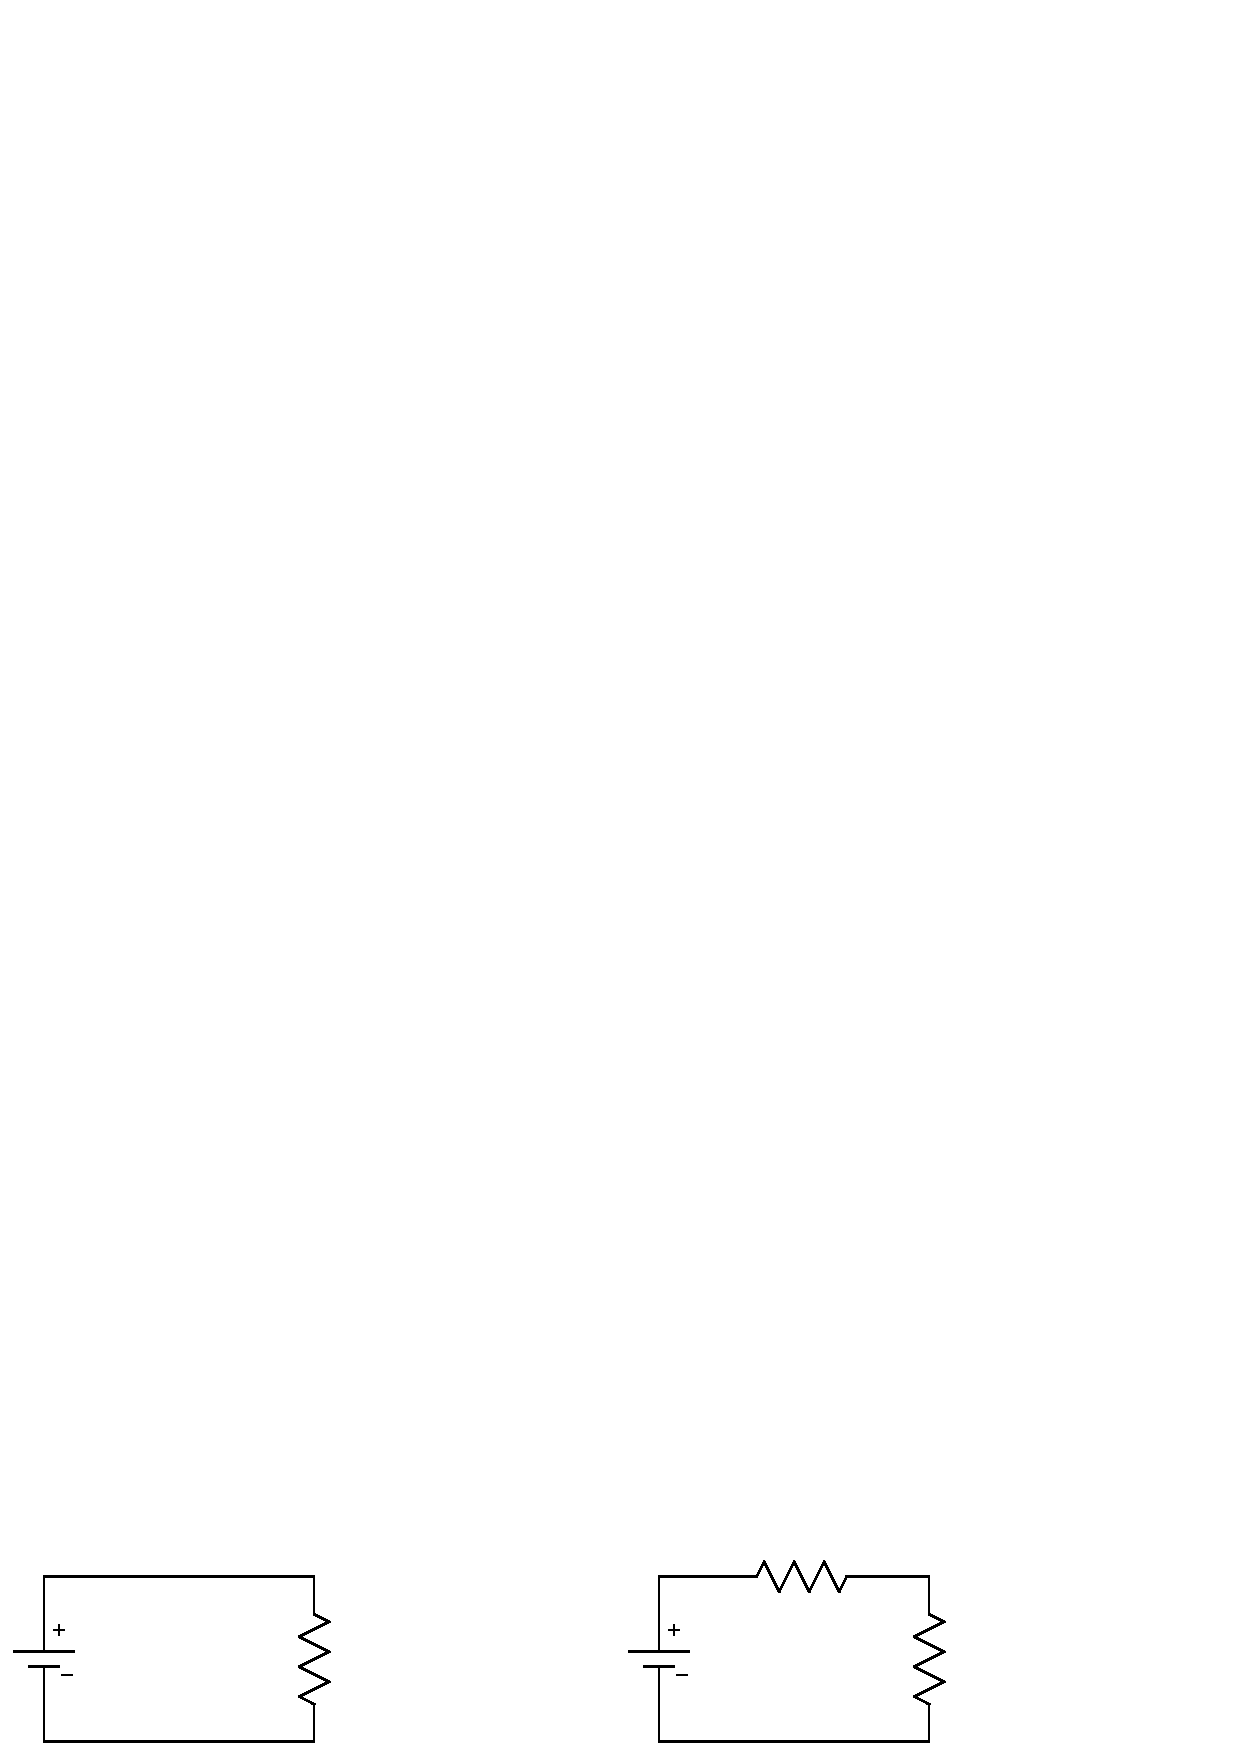
\includegraphics{figMagneticCircuitsCurrentDensityAndElectricFieldIntensity}
\caption{کثافتِ برقی رو اور برقی دباؤ کی شدت}
\label{شکل_مقناطیسی_دور_کثافت_رو_اور_برقی_شدت}
\end{figure}

شکل \حوالہ{شکل_مقناطیسی_دور_کثافت_رو_اور_برقی_شدت} سے ظاہر ہے کہ برقی رو \عددیء{i} سلاخ کی رقبہ عمودی تراش \عددیء{A} سے گزرتی ہے لہٰذا مساوات \حوالہ{مساوات_مقناطیسی_دور_کثافت_رو} کے تحت \عددیء{J} برقی رو کی کثافت کو ظاہر کرتی ہے لہٰذا \عددیء{J} کو \اصطلاح{کثافتِ برقی رو}\فرہنگ{کثافت!برقی رو}\حاشیہب{current density} کہتے ہیں۔ اسی طرح مساوات \حوالہ{مساوات_مقناطیسی_دور_برقی_شدت}   سے  واضح ہے کہ \عددیء{E} برقی دباؤ فی اکائی لمبائی کو ظاہر کرتی ہے لہٰذا  \عددیء{E} کو \اصطلاح{برقی میدان کی شدت}\فرہنگ{برقی میدان!شدت}\حاشیہب{electric field intensity} یا (جہاں متن سے مقناطیسی میدان واضح ہو) مختصراً \اصطلاح{میدانی شدت}  کہتے ہیں۔

	بالکل اسی طرح کی مساواتیں مقناطیسی متغیرات کے لئے حصہ \حوالہ{حصہ_برقی_دور_کثافت_مقناطیسی_بہاو_اور_میدان}  میں لکھی جائیں گی۔  

\حصہ{برقی ادوار}
	برقی دور میں \اصطلاح{برقی دباؤ}\فرہنگ{برقی دباؤ}\حاشیہب{electric voltage}  \عددیء{v}\حاشیہد{برقی دباؤ کی اکائی وولٹ ہے جو اٹلی کے الِسانڈرو وولٹا کے نام ہے جنہوں نے برقی بیٹری ایجاد کی۔}  کی وجہ سے \اصطلاح{برقی رو}\فرہنگ{برقی رو}\حاشیہب{electric current} \عددیء{i} \حاشیہد{برقی رو کی اکائی ایمپیئر ہے جو فرانس کے انڈرِ میرِ ایمپیئر کے نام ہے جن کا برقی و مقناطیسی میدان میں اہم کردار ہے۔} پیدا ہوتی ہے۔ تانبا\فرہنگ{تانبا}\حاشیہب{copper}   کی موصلیت \عددیء{\sigma=\SI{5.9e7}{\siemens \per \meter}} ہے جو بہت بڑی مقدار ہے۔ \عددیء{\si{\siemens \per \meter}} موصلیت کی اکائی ہے۔ تانبا کی موصلیت کی مقدار بہت بڑی ہونے کی بنا اس سے بنی تار کی مزاحمت\حاشیہد{مزاحمت کی اکائی اوہم ہے جو جرمنی کے جارج سائمن اوہم کے نام ہے جنہوں نے قانونِ اوہم دریافت کیا۔}  \عددیء{R_{\textup{تار}}}  عموماً قابلِ نظرانداز ہو گی۔  تار میں برقی رو \عددیء{i} گزرنے سے تار کے سروں کے بیچ برقی دباؤ  \عددیء{\Delta v=i R_{\textup{تار}}} پیدا ہو گا جس کو  \عددیء{R_{\textup{تار}}\to 0} کی بنا  نظر انداز کیا جا سکتا ہے۔یوں تانبے کی تار میں برقی دباو کے گھٹاو کو رد کیا جا سکتا ہے یعنی ہم \عددیء{\Delta v \to 0} لے سکتے ہیں۔ 

شکل \حوالہ{شکل_مقناطیسی_دور_سلسہ_وار_مزاحمتی_ادوار}-الف میں ایک ایسا ہی برقی دور دکھایا گیا ہے جس  میں تانبے کی تار کی مزاحمت کو اکٹھے کر کے ایک ہی جگہ  \عددیء{R_{\textup{تار}}} دکھایا گیا ہے۔اس دور کے لئے درج ذیل لکھا جا سکتا ہے۔
\begin{align}
v&=\Delta v+v_L
\end{align}
تار میں برقی گھٹاو \عددیء{\Delta v} نظرانداز کرتے ہوئے
\begin{align}
v&=v_L
\end{align}
حاصل ہوتا ہے۔اس کا مطلب ہے کہ اگر تار میں برقی دباؤ کا گھٹاو قابل نظرانداز ہو تب لاگو برقی دباؤ جوں کا توں مزاحمت \عددیء{R_L} تک پہنچتا ہے۔برقی ادوار حل کرتے ہوئے یہی حقیقت بروئے کار لاتے ہوئے تار میں برقی دباؤ کے گھٹاو کو نظرانداز کیا جاتا ہے۔شکل \حوالہ{شکل_مقناطیسی_دور_سلسہ_وار_مزاحمتی_ادوار}-الف میں ایسا کرنے سے  شکل \حوالہ{شکل_مقناطیسی_دور_سلسہ_وار_مزاحمتی_ادوار}-ب حاصل ہوتا ہے۔یہاں یہ سمجھ لینا ضروری ہے کہ برقی تار کو اس غرض سے استعمال کیا جاتا ہے کہ لاگو برقی دباؤ کو مقام استعمال تک بغیر گھٹائے پہنچایا جائے۔
\begin{figure}
\centering
\includegraphics[width=\linewidth]{figMagneticCircuitsResistiveSeriesCircuit}
\caption{برقی دور میں تار کی مزاحمت کو نظر انداز کیا جاتا ہے۔}
\label{شکل_مقناطیسی_دور_سلسہ_وار_مزاحمتی_ادوار}
\end{figure}
%---------------------
\begin{figure}
\centering
\includegraphics{figMagneticCircuitsResistiveParallelCircuit}
\caption{کم مزحمتی راہ میں برقی رو کی مقدار زیادہ ہو گی۔}
\label{شکل_مقناطیسی_دور_متوازی_مزاحمتی_دور}
\end{figure}
%

شکل \حوالہ{شکل_مقناطیسی_دور_متوازی_مزاحمتی_دور}  میں ایک اور مثال دی گئی ہے۔ یہاں ہم دیکھتے ہیں کہ برقی رو اس راستے زیادہ ہوتی ہے جس کی مزاحمت کم ہو۔ لہٰذا اگر \عددیء{R_1 < R_2}ہو تب \عددیء{i_1>i_2} ہو گا۔

\حصہ{مقناطیسی دور حصہ اول}
مقناطیسی ادوار بالکل برقی ادوار کی طرح ہوتے ہیں۔ بس ان میں برقی دباؤ \عددیء{v} کی جگہ \اصطلاح{مقناطیسی دباؤ}\فرہنگ{مقناطیسی دباؤ}\حاشیہب{magnetomotive force, mmf}\فرہنگ{mmf} \عددیء{\tau} ، برقی رو \عددیء{i}  کی جگہ \اصطلاح{مقناطیسی بہاو}\فرہنگ{مقناطیسی بہاو}\حاشیہب{flux}\فرہنگ{flux} \عددیء{\phi}  اور مزاحمت \عددیء{R} کی جگہ  \اصطلاح{ہچکچاہٹ}\فرہنگ{ہچکچاہٹ}\حاشیہب{reluctance}  \عددیء{\Re} پائے جاتے ہیں۔ یوں  بالکل برقی ادوار کی طرح مقناطیسی ادوار بنائے جا سکتے ہیں۔  ایک ایسا دور شکل \حوالہ{شکل_مقناطیسی__مقناطیسی_سلسلہ_وار_دور}-الف میں دکھایا گیا ہے۔
\begin{figure}
\centering
\includegraphics{figMagneticCircuitsReluctanceSeriesCircuit}
\caption{مقناطیسی دور}
\label{شکل_مقناطیسی__مقناطیسی_سلسلہ_وار_دور}
\end{figure}
%
یہاں بھی کوشش یہی ہے کہ کسی طرح مقناطیسی دباؤ \عددیء{\tau} کو بغیر گھٹائے ہچکچاہٹ \عددیء{\Re_a} تک پہنچایا جائے۔ عموماً \عددیء{\Re_a} خلائی درز کی ہچکچاہٹ ہوتی ہے اور \عددیء{\Re_c} مقناطیسی قالب کی۔ یہاں بھی اگر \عددیء{\Re_c} قابل نظرانداز ہو تب شکل \حوالہ{شکل_مقناطیسی__مقناطیسی_سلسلہ_وار_دور}-ب حاصل ہو گا جس میں مقناطیسی بہاو \عددیء{\phi}، بالکل اوہم کے قانون کی طرح، درج ذیل مساوات سے حاصل ہو گا۔
\begin{align}
\tau=\phi \Re_a
\end{align}
اگر \عددیء{\Re_c} کو نظرانداز کرنا ممکن نہ ہو تب بالکل سلسلہ وار مزاحمتوں کی طرح ہم  دو سلسلہ وار ہچکچاہٹوں کا مجموعی ہچکچاہٹ  \عددیء{\Re_s}  استعمال کر کے برقی رو حاصل کریں گے، یعنی
\begin{align}
\Re_s&=\Re_a+\Re_c\\
\tau&=\phi \Re_s \label{مساوات_مقناطیسی_دور_مقناطیسی_اوہم_قانون}
\end{align}
برقی دور کی طرح، مقناطیسی دباؤ کو کم ہچکچاہٹ والی راہ سے مقام ضرورت تک پہنچایا جاتا ہے۔ مساوات \حوالہ{مساوات_مقناطیسی_دور_ہچکچاہٹ_کی_تعریف}   کے تحت  ہچکچاہٹ کی قیمت  مقناطیسی مستقل \عددیء{\mu} پر منحصر ہے ۔مقناطیسی مستقل کی اکائی\حاشیہب{Henry per meter}  ہینری فی میٹر \عددیء{\si{\henry \per \meter}} ہے۔\عددیء{\mu} کو عموماً \عددیء{\mu=\mu_r \mu_0} لکھا جاتا ہے جہاں  \عددیء{\mu_0=4 \pi \times 10^{-7}} ہینری فی میٹر کے برابر ہے اور \عددیء{\mu_r} کو \اصطلاح{جزو مقناطیسی مستقل}\فرہنگ{مقناطیسی مستقل!جزو}\حاشیہب{relative permeability, relative magnetic constant} کہتے ہیں۔ لوہا،  کچھ دھاتیں اور چند جدید مصنوعی مواد  ایسی ہیں جن کی \عددیء{\mu_r} کی قیمت \عددیء{\num{2000}} اور \عددیء{\num{80000}} کے  بیچ پائی جاتی ہیں۔ مقناطیسی دباؤ کو  ایک جگہ سے دوسری جگہ منتقل کرنے کے لئے انہی مقناطیسی مواد کو  استعمال کیا جاتا ہے۔ بد قسمتی سے  مقناطیسی مواد کے  \عددیء{\mu} کی مقدار اتنی زیادہ  نہیں ہوتی ہے کہ ان سے بنی سلاخ کی ہچکچاہٹ ہر موقع پر قابل نظرانداز ہو۔ مساوات \حوالہ{مساوات_مقناطیسی_دور_ہچکچاہٹ_کی_تعریف}  کے تحت  ہچکچاہٹ کم سے کم کرنے کی خاطر رقبہ عمودی تراش کو زیادہ سے زیادہ اور لمبائی کو کم سے کم  کرنا ہو گا۔ یوں مقناطیسی دباؤ منتقل کرنے کے لئے  باریک تار نہیں بلکہ خاصی زیادہ رقبہ عمودی تراش کا مقناطیسی راستہ  درکار ہوتا ہے۔مقناطیسی مشین، مثلاً موٹر اور ٹرانسفارمر، کا بیشتر حصہ مقناطیسی دباؤ منتقل کرنے والے ان مقناطیسی مواد  پر مشتمل ہوتا ہے۔ایسے مشینوں کے قلب میں عموماً یہی مقناطیسی مادہ پایا جاتا ہے لہٰذا ایسا مواد  \اصطلاح{مقناطیسی قالب}\فرہنگ{مقناطیسی قالب}\حاشیہب{magnetic core}\فرہنگ{magnetic core} کہلاتا ہے (شکل \حوالہ{شکل_مقناطیسی__کثافت_مقناطیسی_بہاو_اور_شدت})۔برقی مشینوں میں استعمال  مقناطیسی قالب لوہے کی باریک چادر یا پتری\فرہنگ{پتری}\حاشیہب{laminations}\فرہنگ{laminations}  تہہ  در تہہ رکھ کر بنائی جاتی ہے۔ مقناطیسی قالب کے بارے میں مزید معلومات حصہ \حوالہ{حصہ_مقناطیسی_دور_مقناطیسی_مادہ_کے_خصوصیات}  میں  فراہم کی جائے گی۔

\حصہ{کثافتِ مقناطیسی بہاو  اور مقناطیسی میدان کی شدت}\شناخت{حصہ_برقی_دور_کثافت_مقناطیسی_بہاو_اور_میدان}
حصہ \حوالہ{حصہ_برقی_دور_کثافت_برقی_رو_اور_میدان}  میں  برقی دور کی مثال دی گئی۔یہاں شکل \حوالہ{شکل_مقناطیسی__کثافت_مقناطیسی_بہاو_اور_شدت} میں دکھائے گئے مقناطیسی دور پر غور کرتے ہیں۔  مقناطیسی قالب کی \عددیء{\mu_r = \infty} تصور کرتے ہیں۔ یوں  قالب کی ہچکچاہٹ \عددیء{\Re_c} صفر ہو گی۔ حصہ \حوالہ{حصہ_برقی_دور_کثافت_برقی_رو_اور_میدان}   میں تانبا کی تار کی طرح یہاں  مقناطیسی قالب کو مقناطیسی دباؤ \عددیء{\tau} ایک مقام سے دوسری مقام تک منتقل کرنے کے لئے استعمال کیا گیا ہے۔ شکل \حوالہ{شکل_مقناطیسی__کثافت_مقناطیسی_بہاو_اور_شدت} میں مقناطیسی دباؤ کو خلائی درز کی ہچکچاہٹ \عددیء{\Re_a} تک پہنچایا گیا ہے۔
\begin{figure}
\centering
\includegraphics{figMagneticCircuitsMagneticFluxDensityAndIntensity}
\caption{کثافتِ مقناطیسی بہاو اور مقناطیسی میدان کی شدت۔}
\label{شکل_مقناطیسی__کثافت_مقناطیسی_بہاو_اور_شدت}
\end{figure}
لہٰذا یہاں کُل ہچکچاہٹ صرف خلائی درز کی ہچکچاہٹ ہی ہے یعنی:
\begin{align}
\Re_a=\frac{l_a}{\mu_0 A_a}
\end{align}
اگر خلائی درز کی لمبائی \عددیء{l_a} قالب کے رقبہ عمودی تراش کے اضلاع \عددیء{b} اور \عددیء{w} سے بہت کم ہوں، یعنی \عددیء{l_a \ll b} اور \عددیء{l_a \ll w} تب خلائی درز کے رقبہ عمودی تراش \عددیء{A_a} کو قالب کے رقبہ عمودی تراش \عددیء{\Re_c} کے برابر لیا جاتا ہے، یعنی:
\begin{align}
A_a=A_c=w b
\end{align}
 اس کتاب میں جہاں بتلایا نہ گیا ہو وہاں \عددیء{l_a \ll b} اور \عددیء{l_a \ll w} تصور کرتے ہوئے \عددیء{A_a=A_c} لیا جائے گا۔
 
مقناطیسی دباؤ \عددی{\tau} کی تعریف درج ذیل مساوات  پیش کرتی ہے۔
\begin{align}
\tau=N i
\end{align}
یوں برقی تار کے چکر ضرب تار میں برقی رو کو مقطاطیسی دباو کہتے ہیں۔ مقناطیسی دباؤ کی اکائی \اصطلاح{ایمپیئر-چکر}\فرہنگ{ایمپیئر-چکر}\حاشیہب{ampere-turn}\فرہنگ{ampere-turn}  ہے۔ بالکل حصہ \حوالہ{حصہ_برقی_دور_کثافت_برقی_رو_اور_میدان}   کی طرح ہم مساوات \حوالہ{مساوات_مقناطیسی_دور_مقناطیسی_اوہم_قانون} کو یوں لکھ سکتے ہیں۔
\begin{align}\label{مساوات_مقناطیسی_ڈور_بہاو_مساوی_دباؤ_بٹا_ہچکچاہٹ}
\phi_a=\frac{\tau}{\Re_a}
\end{align}
مقناطیسی بہاو کی اکائی\فرہنگ{ویبر}\حاشیہب{Weber}\فرہنگ{Weber} \اصطلاح{ویبر}\حاشیہد{یہ اکائی جرمنی کے ولیم اڈورڈ ویبر کے نام ہے جن کا برقی و مقناطیسی میدان میں اہم کردار رہا ہے}  ہے اور ہچکچاہٹ کی اکائی \اصطلاح{ایمپیئر-چکر فی ویبر}\حاشیہب{ampere-turn per weber} ہے۔ اس سلسلہ وار دور کی خلائی درز میں مقناطیسی بہاو \عددیء{\phi_a} اور قالب میں مقناطیسی بہاو \عددیء{\phi_c} ایک دوسرے کے برابر ہوں گے۔درج بالا مساوات کو مساوات \حوالہ{مساوات_مقناطیسی_دور_ہچکچاہٹ_کی_تعریف}   کی مدد سے
\begin{align}
\phi_a &=\tau \left(\frac{\mu_0 A_a}{l_a} \right) \nonumber \\
\intertext{یا}
\frac{\phi_a}{A_a}&=\mu_0 \left( \frac{\tau}{l_a} \right) \label{مساوات_مقناطیسی_دور_کثافت_بہاو_اوہم_قانون_سے}
\end{align}
 لکھ سکتے ہیں جہاں درز کی نشاندہی زیر نوشت میں \عددی{a} لکھ کر کی گئی ہے۔ اس مساوات میں بائیں ہاتھ مقناطیسی بہاو فی اکائی رقبہ کو \اصطلاح{کثافتِ مقناطیسی بہاو}\فرہنگ{مقناطیسی بہاو!کثافت}\حاشیہب{magnetic flux density}\فرہنگ{magnetic flux!density} \عددیء{B_a} اور دائیں ہاتھ مقناطیسی دباؤ فی اکائی لمبائی کو \اصطلاح{مقناطیسی میدان کی شدت}\فرہنگ{مقناطیسی میدان!شدت}\حاشیہب{magnetic field intensity}\فرہنگ{magnetic field!intensity}  \عددیء{H_a} لکھا جا سکتا ہے، یعنی:
\begin{align}
B_a&=\frac{\phi_a}{A_a}\\
H_a&=\frac{\tau}{l_a}
\end{align}
کثافتِ مقناطیسی بہاو کی اکائی \اصطلاح{ویبر فی مربع میٹر} ہے جس کو \اصطلاح{ٹسلا}\فرہنگ{ٹسلا}\فرہنگ{Tesla}\حاشیہد{Tesla:  یہ اکائی سربیا کے نِکولا ٹسلا کے نام ہے جنہوں نے بدلتی رو برقی طاقت عام کرنے میں اہم کردار ادا کیا}  کا نام دیا گیا ہے۔مقناطیسی میدان کی شدت کی اکائی \اصطلاح{ایمپیئر فی میٹر}\حاشیہب{ampere per meter}  ہے۔ یوں مساوات \حوالہ{مساوات_مقناطیسی_دور_کثافت_بہاو_اوہم_قانون_سے} کو درج ذیل لکھا جا سکتا ہے۔
\begin{align}
B_a=\mu_0 H_a
\end{align}
جہاں متن سے واضح ہو کہ مقناطیسی میدان کی بات ہو رہی ہے وہاں مقناطیسی میدان کی شدت کو مختصراً \اصطلاح{میدانی شدت}\حاشیہب{field intensity} کہا جاتا ہے۔  شکل \حوالہ{شکل_مقناطیسی__کثافت_مقناطیسی_بہاو_اور_شدت} میں ہم دیکھتے ہیں کہ خلائی درز میں مقناطیسی بہاو کا رخ  اکائی سمتیہ \عددیء{\az} کے  ہے لہٰذا ہم کثافتِ مقناطیسی بہاو کو \عددیء{\kvec{B_a}=-B_a \az} لکھ سکتے ہیں۔ اسی طرح خلائی درز میں مقناطیسی دباؤ  اکائی سمتیہ \عددیء{\az} کی الٹ رخ دباؤ ڈال رہا ہے لہٰذا ہم مقناطیسی دباؤ کی شدت کو \عددیء{\kvec{H_a}=-H_a \az} لکھ سکتے ہیں۔ یوں درج بالا مساوات کو درج ذیل لکھا جا سکتا ہے۔
\begin{align}
\kvec{B_a}=\mu_0 \kvec{H_a}
\end{align}
اگر خلاء کی جگہ کوئی اور مادہ ہو تب ہم اس مساوات کو درج ذیل لکھتے۔
\begin{align}
\kvec{B}=\mu \kvec{H}
\end{align}
%
\ابتدا{مثال}
شکل \حوالہ{شکل_مقناطیسی__کثافت_مقناطیسی_بہاو_اور_شدت} میں خلائی درز میں کثافتِ مقناطیسی بہاو \عددیء{0.1} ٹسلا درکار ہے۔قالب کی \عددیء{\mu_r=\infty}  ہے اور خلائی درز کی لمبائی \عددیء{1} ملی میٹر ہے۔اگر  قالب کے گرد برقی تار کے \عددیء{100} چکر ہوں تب درکار برقی رو \عددی{i} کتنا ہو گا۔

حل:
\begin{align*}
\tau&=\phi \Re\\
N i &= \phi \left(\frac{l}{\mu_0 A} \right)\\
\frac{\phi}{A}&=B=\frac{ N i \mu_0}{l}
\end{align*}
لہٰذا
\begin{align*}
0.1&=\frac{100 \times i \times 4 \pi  10^{-7}}{0.001}\\
i&=\frac{0.1 \times 0.001}{100 \times 4 \pi  10^{-7}}=\SI{0.79567}{\ampere}
\end{align*}
\عددیء{i=\SI{0.79567}{\ampere}} برقی رو  خلائی درز میں \عددیء{B=\SI{0.1}{\tesla}} کثافتِ مقناطیسی بہاو پیدا کرے گا۔
\انتہا{مثال}
%
\حصہ{مقناطیسی دور حصہ دوم}
شکل \حوالہ{شکل_مقناطیسی__سادہ_مقناطیسی_دور_بغیر_درز} میں ایک سادہ مقناطیسی نظام دکھایا گیا ہے جس میں قالب کی مقناطیسی مستقل کو محدود تصور کرتے ہیں۔مقناطیسی دباؤ  \عددیء{\tau=N i} مقناطیسی قالب میں مقناطیسی بہاو \عددیء{\phi_c} پیدا کرتا ہے۔ قالب کا رقبہ عمودی تراش \عددیء{A_c}  ہر جگہ ایک یکساں ہے اور قالب  کی اوسط لمبائی \عددیء{l_c} ہے۔ قالب میں مقناطیسی بہاو  کا رخ  \اصطلاح{فلیمنگ}\حاشیہب{Fleming's right hand rule} کے دائیں ہاتھ کے قانون  سے معلوم کیا جا سکتا ہے۔اس قانون کو دو طریقوں سے بیان کیا جا سکتا ہے۔
\begin{itemize}
\item
اگر ایک لچھے کو دائیں ہاتھ سے یوں پکڑا  جائے کہ ہاتھ کی چار انگلیاں لچھے میں برقی رو کے رخ لپٹی  ہوں تب انگوٹھا اُس مقناطیسی بہاو کے رخ ہو گا جو اس برقی رو کی وجہ سے وجود میں آیا ہو۔
\item
اگر ایک تار جس میں برقی رو کا گزر ہو کو دائیں ہاتھ سے یوں پکڑا جائے کہ انگوٹھا  برقی رو  کے رخ ہو تب باقی چار انگلیاں اُس مقناطیسی  بہاو کے رخ لپٹی ہوں گی  جو اس برقی رو کی وجہ سے  پیدا ہوگا۔
\end{itemize}

ان دو بیانات میں پہلا بیان  لچھے میں مقناطیسی بہاو کا رخمعلوم کرنے کے لئے زیادہ آسان ثابت ہوتا ہے جبکہ  سیدھی تار کے گرد مقناطیسی بہاو کا رخ دوسرے بیان سے زیادہ آسانی سے معلوم کیا جا سکتا ہے۔
\begin{figure}
\centering
\includegraphics{figMagneticCircuitsSimpleMagneticCircuitNoGap}
\caption{سادہ مقناطیسی دور۔}
\label{شکل_مقناطیسی__سادہ_مقناطیسی_دور_بغیر_درز}
\end{figure}

قالب میں مقناطیسی بہاو  گھڑی کے سمت میں ہے۔ مقناطیسی بہاو \عددی{\phi} کو  شکل \حوالہ{شکل_مقناطیسی__سادہ_مقناطیسی_دور_بغیر_درز} میں تیر والے ہلکی سیاہی کے لکیر  سے ظاہر کیا گیا ہے۔ قالب کی ہچکچاہٹ 
\begin{align*}
\Re_c&=\frac{l_c}{\mu_c A_c}
\end{align*}
لکھتے ہوئے مقناطیسی بہاو 
\begin{align*}
\phi_c&=\frac{\tau}{\Re_c}=N i \left(\frac{\mu_c A_c}{l_c} \right)
\end{align*}
ہو گا۔اس طرح ہم  تمام نا معلوم متغیرات حاصل کر پائے ہیں۔
%
\ابتدا{مثال}
شکل \حوالہ{شکل_مقناطیسی__درز_اور_ہچکچاہٹ}  میں ایک مقناطیسی قالب دکھایا گیا ہے جس کی معلومات درج ذیل ہے۔
\begin{align}
\text{قالب}= \left\{ 
  \begin{array}{l l}
  h=\SI{20}{\centi\meter} & m=\SI{10}{\centi \meter}\\
 n=\SI{8}{\centi\meter} & w=\SI{2}{\centi \meter}\\
 l_a=\SI{1}{\milli\meter} & \mu_r =\num{40000} \\
 \end{array} \right.
\end{align}
قالب اور خلائی درز کی ہچکچاہٹیں حاصل کریں۔
\begin{figure}
\centering
\includegraphics{figMagneticCircuitsCoreWithGapAndReluctance}
\caption{خلائی درز اور قالب کے ہچکچاہٹ۔}
\label{شکل_مقناطیسی__درز_اور_ہچکچاہٹ}
\end{figure}

حل:
\begin{align*}
b&=\frac{m-n}{2}=\frac{0.1-0.08}{2}=\SI{0.01}{\meter}\\
A_a&=A_c=bw=0.01 \times 0.02=\SI{0.0002}{\square \meter}\\
l_c&=2(h+n)-l_a=2(0.2+0.08)-0.001=\SI{0.559}{\meter}
\end{align*}
%
\begin{align*}
\Re_c&=\frac{l_c}{\mu_r \mu_0 A_c}=\frac{0.559}{40000 \times 4 \pi 10^{-7} \times 0.0002}=\SI{55598}{\ampere \cdot t \per \weber}\\
\Re_a&=\frac{l_a}{\mu_0 A_a}=\frac{0.001}{4 \pi 10^{-7} \times 0.0002}=\SI{3978358}{\ampere \cdot t \per \weber}
\end{align*}
ہم دیکھتے ہیں اگرچہ قالب کی لمبائی خلائی درز کی لمبائی سے \عددیء{559} گنا زیادہ ہے تب بھی خلائی درز کی ہچکچاہٹ \عددیء{71} گنا زیادہ ہے۔یوں  \عددیء{\Re_a  \gg \Re_c} ہو گا۔
\انتہا{مثال}
%
\ابتدا{مثال}
شکل  \حوالہ{شکل_مقناطیسی_دور_سادہ_گھومتا_مشین} سے رجوع کریں۔خلائی درز \عددیء{5} ملی میٹر لمبا ہے اور گھومتے حصہ پر \عددیء{1000} چکر ہیں۔خلائی درز میں \عددیء{\SI{0.95}{\tesla}} کثافتِ برقی بہاو حاصل کرنے کی خاطر درکار برقی رو معلوم کریں۔
\begin{figure}
\centering
\includegraphics{figMagneticCircuitsSimpleRotatingMachineOutline}
\caption{سادہ گھومنے والا مشین}
\label{شکل_مقناطیسی_دور_سادہ_گھومتا_مشین}
\end{figure}

حل:\quad
اس شکل میں گھومتے مشین، مثلاً موٹر، کی ایک سادہ صورت دکھائی گئی ہے۔ ایسی مشینوں کا بیرونی حصہ ساکن رہتا ہے لہٰذا اس حصے  کو مشین کا \اصطلاح{ساکن حصہ}\فرہنگ{ساکن حصہ}\حاشیہب{stator}\فرہنگ{stator} کہتے ہیں۔ساکن حصے کے اندر مشین کا  گھومتا حصہ پایا جاتا ہے لہٰذا اس حصے کو مشین کا \اصطلاح{گھومتا حصہ}\فرہنگ{گھومتا حصہ}\حاشیہب{rotor}\فرہنگ{rotor} کہتے ہیں۔ اس مثال میں ان دونوں حصوں کا  \عددیء{\mu_r=\infty}  ہے لہٰذا ان کی ہچکچاہٹ صفر ہو گی۔ مقناطیسی بہاو  کو ہلکی سیاہی کی لکیر سے ظاہر کیا گیا ہے۔ مقناطیسی بہاو کی ایک مکمل چکر کے دوران مقناطیسی بہاو دو خلائی درزوں  سے گزرتا ہے۔ یہ دو خلائی درز ہر لحاظ سے ایک جیسے ہیں لہٰذا ان دونوں خلائی درز کی ہچکچاہٹ بھی ایک دوسرے کے برابر ہوں گی۔مزید دونوں خلائی درزوں کی ہچکچاہٹ سلسلہ وار ہیں۔شکل \حوالہ{شکل_مقناطیسی_دور_سادہ_گھومتا_مشین} میں مقناطیسی بہاو کو گھومتے حصہ، ساکن حصہ اور دو خلائی درزوں  سے گزرتا ہوا دکھایا گیا ہے۔خلائی درز کی لمبائی \عددیء{l_a} بہت کم ہے لہٰذا خلائی درز کا عمودی رقبہ تراش \عددیء{A_a} وہی ہو گا جو گھومتے حصہ کا ہے یعنی \عددیء{A_a=A_c} ہو گا۔

ایک خلائی درز کی ہچکچاہٹ
\begin{align*}
\Re_a=\frac{l_a}{\mu_0 A_a}=\frac{l_a}{\mu_0 \A_c}
\end{align*}
ہے لہٰذا دو سلسلہ وار خلائی درزوں کی کُل ہچکچاہٹ درج ذیل ہو گی۔
\begin{align*}
\Re_s=\Re_a=\Re_a=\frac{2 l_a}{\mu_0 A_c}
\end{align*}
خلائی درز میں مقناطیسی بہاو \عددیء{\phi_a} اور کثافتِ مقناطیسی بہاو \عددیء{B_a} درج ذیل ہوں گے۔
\begin{align*}
\phi_a&=\frac{\tau}{\Re_s}=\left(N i \right) \left (\frac{\mu_0 A_c}{2 l_a} \right)\\
B_a&=\frac{\phi_a}{A_a}=\frac{\mu_0 N i}{2 l_a}
\end{align*}
اس مساوات میں اعداد استعمال کرتے ہیں۔
\begin{align*}
0.95&=\frac{4 \pi 10^{-7} \times 1000 \times i}{2 \times 0.005}\\
i&=\frac{0.95 \times 2 \times 0.005}{ 4 \pi 10^{-7} \times 1000}=\SI{7.56}{\ampere}
\end{align*}
موٹر اور جنریٹروں کی خلاء میں تقریباً ایک ٹسلا کثافتِ برقی بہاو ہوتی ہے۔
\انتہا{مثال}

\حصہ{خود امالہ  ، مشترکہ امالہ  اور توانائی}
مقناطیسی بہاو کی وقت کے ساتھ تبدیلی برقی دباؤ  کو جنم دیتی ہے۔ لہٰذا  اگر شکل \حوالہ{شکل_مقناطیسی__کثافت_مقناطیسی_بہاو_اور_شدت}  کے قالب میں مقناطیسی بہاو تبدیل ہو رہی ہو تو اس کی وجہ سے اس کے لچھے میں برقی دباؤ پیدا ہو گا جو کہ اس لچھے کے سروں پر نمودار ہو گا۔ اِس طرح پیدا ہونے والی برقی دباؤ کو \اصطلاح{امالی برقی دباؤ}\فرہنگ{امالی برقی دباؤ}\حاشیہب{induced voltage}\فرہنگ{induced voltage}  کہتے ہیں۔ \اصطلاح{قانونِ فیراڈے}\فرہنگ{فیراڈے!قانون}\حاشیہب{Faraday's law}\فرہنگ{Faraday's law}  کے تحت\حاشیہد{مائکل فیراڈے انگلستانی سائنسدان تھے جنہوں نے محرک برقی دباؤ دریافت کی}
\begin{align}\label{مساوات_مقناطیسی_دور_فیراڈے_قانون}
e=N \frac{\partial \phi}{\partial t} =\frac{\partial \lambda}{\partial t}
\end{align}
اس مساوات میں ہم لچھے میں، وقت کے ساتھ تبدیل ہونے والی، مقناطیسی بہاو کو \عددیء{\phi} سے ظاہر کر رہے ہیں۔\عددیء{N \phi} کو لچھے کی \اصطلاح{ارتباط بہاو}\فرہنگ{ارتباط بہاو}\حاشیہب{flux linkage} \عددیء{\lambda}  کہتے ہیں جس کی اکائی \اصطلاح{ویبر-چکر}\فرہنگ{ویبر-چکر}\حاشیہب{weber-turn}  ہے۔ اس امالی برقی دباؤ  کی سمت کا تعین یوں کیا جاتا ہے کہ اگر دیئے گئے لچھے کی سروں کو \اصطلاح{کسرِ دور}\فرہنگ{کسر دور}\حاشیہب{short circuit}   کیا جائے تو اِس میں برقی رو اُس سمت میں ہو گی جس میں مقناطیسی بہاو کی تبدیلی کو روکا جا سکے۔ 

جن مقناطیسی دوروں میں مقناطیسی مستقل \عددیء{\mu}  کو اٹل مقدار تصور کیا جا سکے یا جن میں خلائی درز کی ہچکچاہٹ قالب کی ہچکچاہٹ سے بہت زیادہ ہو یعنی \عددیء{\Re_a \gg \Re_c} ، ان حالات میں ہم لچھے کی  \اصطلاح{امالہ}\فرہنگ{امالہ}\حاشیہب{inductance}\فرہنگ{inductance} \عددیء{L}  کو یوں بیان کرتے ہیں۔
\begin{align}\label{مساوات_مقناطیسی_دور_خود_امالہ_تعریف}
L=\frac{\lambda}{i}
\end{align}

امالہ کی اکائی ویبر-چکر فی ایمپیئر ہے جس کو \اصطلاح{ہینری}\فرہنگ{Henry}\حاشیہب{Henry}\فرہنگ{Henry} \عددیء{H} کا نام\حاشیہد{امریکی سائنسدان جوزف ہینری جنہوں نے مائکل فیراڈے سے علیحدہ  طور پر محرک برقی دباؤ دریافت کی} دیا گیا ہے۔ لہٰذا
\begin{align}
L=\frac{N \phi}{i}=\frac{N B_c A_c}{i}=\frac{N^2 \mu_0 A_a}{l_a}
\end{align}
%
\ابتدا{مثال}
شکل \حوالہ{شکل_مقناطیسی__کثافت_مقناطیسی_بہاو_اور_شدت} میں اگر \عددیء{b=\SI{5}{\centi \meter},w=\SI{4}{\centi\meter},l_a=\SI{3}{\milli \meter}} جبکہ لچھے کے \عددیء{1000} چکر اور قالب کی اوسط لمبائی \عددیء{l_c=\SI{30}{\centi\meter}} ہو تب ان دو صورتوں میں لچھے کی امالہ معلوم کریں۔
\begin{itemize}
\item
قالب کی \عددیء{\mu_r = \infty} ہے۔
\item
قالب کی \عددیء{\mu_r = 500} ہے۔
\end{itemize}

حل:\quad
پہلی صورت میں قالب کی \عددیء{\mu_r=\infty} ہونے کی وجہ سے قالب کی ہچکچاہٹ نظرانداز کی جا سکتی ہے۔یوں
\begin{align*}
L&=\frac{N^2 \mu_0 w b}{l_a}\\
&=\frac{1000^2 \times 4 \pi 10^{-7} \times 0.04 \times 0.05}{0.003}\\
&=\SI{0.838}{\henry}
\end{align*}
	دوسری صورت میں \عددیء{\mu_r=500} ہے۔یوں قالب کی ہچکچاہٹ صفر نہیں۔خلاء اور قالب کی ہچکچاہٹ پہلے دریافت کرتے ہیں
\begin{align*}
\Re_a&=\frac{l_a}{\mu_0 w b}=\frac{0.003}{4\pi 10^{-7} \times 0.04 \times 0.05}=\SI{1193507}{\ampere \cdot t \per \weber}\\
\Re_c&=\frac{l_c}{\mu_r \mu_0 w b}=\frac{0.3}{500 \times 4\pi 10^{-7} \times 0.04 \times 0.05}=\SI{238701}{\ampere \cdot t \per \weber}
\end{align*}
لہٰذا
\begin{align*}
\phi&=\frac{N i}{\Re_a+\Re_c}\\
\lambda &= N \phi = \frac{N^2 i}{\Re_a+\Re_c}\\
L&=\frac{\lambda}{i}=\frac{N^2}{\Re_a+\Re_c}=\frac{1000^2}{\num{1193507}+\num{238701}}=\SI{0.698}{\henry}
\end{align*}
\انتہا{مثال}
%
\ابتدا{مثال}
شکل \حوالہ{شکل_مقناطیسی_ادوار_پیچدار_لچھا} میں ایک پیچدار لچھا\فرہنگ{لچھا!پیچدار}\حاشیہب{spiral coil} دکھایا گیا ہے جس کی تفصیل یوں ہے

\عددیء{N=11, r=\SI{0.49}{\meter},l=\SI{0.94}{\meter}}

ایسے پیچدار لچھے کی بیشتر مقناطیسی بہاو لچھے کے اندر محوری سمت میں ہوتی ہے۔لچھے کے باہر مقناطیسی بہاو کی مقدار قابلِ نظرانداز ہوتی ہے۔یوں لچھے کے اندر محوری جانب مقناطیسی شدت
\begin{align*}
H=\frac{N i}{l}
\end{align*}
ہوتی ہے۔اس لچھے کی خود امالہ حاصل کریں۔
\begin{figure}
\centering
\includegraphics{figMagneticCircuitsCoil}
\caption{پیچدار لچھا}
\label{شکل_مقناطیسی_ادوار_پیچدار_لچھا}
\end{figure}
حل:
\begin{align*}
B&=\mu_0 H=\frac{\mu_0 N i}{l}\\
\phi&=B  \pi r^2=\frac{\mu_0 N i \pi r^2}{l}\\ 
\lambda&=N \phi =\frac{\mu_0 N^2 i \pi r^2}{l}\\ 
L&=\frac{\lambda}{i}=\frac{\mu_0 N^2 \pi r^2}{l}
\end{align*} 
یوں
\begin{align*}
L=\frac{4 \pi 10^{-7} \times 11^2 \times \pi  \times 0.49^2}{0.94}=\SI{122}{\micro \henry}
\end{align*}
یہ پیچدار لچھا میں نے  \عددیء{3000} کلو گرام لوہا پگھلانے والی بھٹی میں استعمال کیا ہے۔
\انتہا{مثال}
%
شکل \حوالہ{شکل_مقناطیسی_ادوار_دو_لچھے_ایک_درز} میں دو لچھے والا ایک مقناطیسی دور دکھایا گیا ہے۔ ایک لچھے کے  \عددیء{N_1} چکر ہیں اور اس میں برقی رو \عددیء{i_1} ہے اور دوسرا لچھا \عددیء{N_2} چکر کا ہے اور اس میں برقی  رو \عددیء{i_2} ہے۔ دونوں لچھوں میں برقی رو کی سمتیں یوں ہیں کہ اِن  دونوں کا مقناطیسی دباؤ جمع ہو۔ یوں اگر قالب کے امالہ کو نظرانداز کیا جائے تو ہم مقناطیسی بہاو \عددیء{\phi} کے لئے لکھ سکتے ہیں
\begin{align}
\phi=\left (N_1 i_1 +N_2 i_2 \right ) \frac{\mu_0 A_a}{l_a}
\end{align} 
%
\begin{figure}
\centering
\includegraphics{figMagneticCircuitsTwoCoilsWithGap}
\caption{دو لچھے والا مقناطیسی دور۔}
\label{شکل_مقناطیسی_ادوار_دو_لچھے_ایک_درز}
\end{figure}
یہاں \عددیء{\phi} دونوں لچھوں کے مجموعی مقناطیسی دباؤ یعنی \عددیء{N_1 i_1+N_2 i_2} سے پیدا ہونے والا مقناطیسی بہاو ہے۔ اس مقناطیسی بہاو  کی ان  لچھوں  کے ساتھ  ارتباط کو یوں لکھا جا سکتا ہے۔
\begin{align}
\lambda_1=N_1 \phi=N_1^2  \frac{\mu_0 A_a}{l_a} i_1 +N_1 N_2  \frac{\mu_0 A_a}{l_a} i_2
\end{align}
اس کو یوں لکھا جا سکتا ہے
\begin{align}\label{مساوات_مقناطیسی_دور_ارتباط_دو_لچھے}
\lambda_1 = L_{11} i_1+L_{12} i_2
\end{align}
جہاں
\begin{align}
L_{11}&=N_1^2  \frac{\mu_0 A_a}{l_a}\\
L_{12}&=N_1 N_2  \frac{\mu_0 A_a}{l_a}
\end{align}
ہیں۔ یہاں \عددیء{L_{11}} پہلے لچھے کی  \اصطلاح{خود امالہ}\فرہنگ{خود امالہ}\حاشیہب{self inductance}\فرہنگ{self inductance}  ہے اور  \عددیء{L_{11} i_1} اِس لچھے کی اپنے برقی رو \عددیء{i_1} سے پیدا مقناطیسی بہاو  کے ساتھ  ارتباط بہاو ہے جسے \اصطلاح{خود ارتباط بہاو}\فرہنگ{خود ارتباط بہاو}\حاشیہب{self flux linkage}\فرہنگ{self flux linkage} کہتے ہیں۔\عددیء{L_{12}}  اِن دونوں لچھوں  کا  \اصطلاح{مشترکہ امالہ}\فرہنگ{مشترکہ امالہ}\حاشیہب{mutual inductance}\فرہنگ{mutual inductance} ہے اور  \عددیء{L_{12} i_2}  لچھا نمبر-1  کے ساتھ برقی رو  \عددیء{i_2} کی وجہ سے  ارتباط بہاو  ہے جسے \اصطلاح{مشترکہ ارتباط بہاو}\فرہنگ{مشترکہ ارتباط امالہ}\حاشیہب{mutual flux linkage}\فرہنگ{mutual flux linkage}  کہتے ہیں ۔ بالکل اسی طرح ہم دوسرے لچھے کے لئے لکھ سکتے ہیں
\begin{align}
\lambda_2&=N_2 \phi=N_2 N_1 \frac{\mu_0 A_a}{l_a} i_1+N_2^2 \frac{\mu_0 A_a}{l_a} i_2  \nonumber \\
&=L_{21} i_1+L_{22} i_2 \label{مساوات_مقناطیسی_دور_دوسرے_لچھے_کی_ارتباط}
\end{align}
جہاں
\begin{align}
L_{22}&=N_2^2 \frac{\mu_0 A_a}{l_a}\\
L_{21}&=L_{12}=N_2 N_1 \frac{\mu_0 A_a}{l_a} \label{مساوات_مقناطیسی_دور_مشترکہ_امالہ_یکساں}
\end{align}
ہیں۔\عددیء{L_{22}} دو نمبر لچھے  کی خود امالہ اور  \عددیء{L_{21}=L_{12}} ان  دو لچھوں کی مشترکہ امالہ ہے۔ یہاں یہ واضح کرنا ضروری ہے کہ امالہ کا تصور اس وقت کارآمد ہوتا جب ہم مقناطیسی مستقل \عددیء{\mu}  کو اٹل تصور کر سکیں۔

مساوات \حوالہ{مساوات_مقناطیسی_دور_خود_امالہ_تعریف}  کو مساوات \حوالہ{مساوات_مقناطیسی_دور_فیراڈے_قانون}  میں استعمال کریں تو 
\begin{align}
e=\frac{\partial \lambda}{\partial t}=\frac{ \partial \left (N \phi \right)}{\partial t}=\frac{\partial \left( L i\right) }{\partial t}
\end{align}
اگر امالہ مقررہ ہو جیسا کہ ساکن آلوں میں ہوتا ہے تب ہمیں  امالہ کی جانی پہچانی مساوات ملتی ہے 
\begin{align}
e=L \frac{\partial i}{\partial t}
\end{align}
مگر اگر امالہ بھی تبدیل ہو جیسا کہ موٹروں اور جنریٹروں میں ہوتا ہے تب
\begin{align}
e= L \frac{\partial i}{\partial t} + i \frac{\partial L}{\partial t}
\end{align}
توانائی\فرہنگ{توانائی}\حاشیہب{energy}\فرہنگ{energy}  کی اکائی \اصطلاح{جاول}\فرہنگ{جاول}\حاشیہب{Joule}\فرہنگ{Joule} \عددیء{J}\حاشیہد{جیمس پریسقوٹ جاول انگلستانی سائنسدان جنہوں نے حرارت اور میکانی کام کا رشتہ دریافت کیا} ہے اور طاقت\فرہنگ{طاقت}\حاشیہب{power}\فرہنگ{power}  کی اکائی\حاشیہد{سکاٹلینڈ کے جیمز واٹ جنہوں نے بخارات پر چلنے والے انجن پر کام کیا} جاول فی سیکنڈ یا \اصطلاح{واٹ}\فرہنگ{واٹ}\حاشیہب{Watt}\فرہنگ{Watt} \عددیء{W}  ہے۔

اس کتاب میں توانائی یا کام کو \عددیء{W} سے ظاہر کیا جائے گا مگر طاقت کی اکائی واٹ \عددیء{W} کے لئے بھی ہی کی علامت استعمال ہوتی ہے۔امید کی جاتی ہے کہ اس سے غلطی پیش نہیں آئے گی اور استعمال کو دیکھ کر یہ فیصلہ کرنا کہ اس کا کونسا مطلب لیا جا رہا ہے دشوار نہ ہو گا۔

وقت کے ساتھ توانائی کی شرح کو طاقت کہتے ہیں لہٰذا کسی لچھے کے لئے ہم لکھ سکتے ہیں
\begin{align}
p=\frac{\dif W}{\dif t} = e i = i \frac{\partial \lambda}{\partial t}
\end{align} 
لہٰذا ایک مقناطیسی دور میں  \عددیء{t_1} سے \عددیء{t_2} تک کے وقفے میں مقناطیسی توانائی میں تبدیلی کو تکمل کے ذریعہ یوں حاصل کیا جا سکتا ہے۔
\begin{align}
\Delta W = \int_{t1}^{t2} p \dif t =\int_{\lambda1}^{\lambda2} i \dif \lambda
\end{align}
اگر مقناطیسی دور میں ایک ہی لچھا ہو اور اس دور میں امالہ اٹل ہو تب
\begin{align}
\Delta W = \int_{\lambda1}^{\lambda2} i \dif \lambda=\int_{\lambda1}^{\lambda2} \frac{\lambda}{L} \dif \lambda=\frac{1}{2 L} \left(\lambda_2^2-\lambda_1^2 \right)
\end{align}

	اگر ہم لمحہ \عددیء{t_1} پہ \عددیء{\lambda_1=0} تصور کریں تب ہم کسی دیئے گئے \عددیء{\lambda} پہ مقناطیسی توانائی کو یوں لکھ سکتے ہیں
\begin{align}
\Delta W=\frac{\lambda^2}{2L}=\frac{L i^2}{2}
\end{align}

\حصہ{مقناطیسی مادہ کے خصوصیات}\شناخت{حصہ_مقناطیسی_دور_مقناطیسی_مادہ_کے_خصوصیات}
مقناطیسی دوروں میں قالب استعمال کرنے سے دو طرح کے فوائد حاصل ہوتے ہیں۔ قالب کے استعمال سے ایک تو کم مقناطیسی دباؤ سے زیادہ مقناطیسی بہاو پیدا کی جا سکتی ہے اور دوسری، مقناطیسی بہاو کو اپنی مرضی کے راستوں پابند کیا جاسکتا ہے۔ ٹرانسفارمروں میں قالب کو استعمال کر کے مقناطیسی بہاو کو اِس طرح پابند کیا جاتا ہے کہ جو مقناطیسی بہاو ایک لچھے سے گزرتا ہے، وہی مقناطیسی بہاو، سارا کا سارا، باقی لچھوں سے بھی گزرتا ہے۔ موٹروں میں قالب کو استعمال کر کے مقناطیسی بہاو کو یوں پابند کیا جاتا ہے کہ زیادہ سے زیادہ قوت پیدا ہو جبکہ جنریٹروں میں اسے زیادہ سے زیادہ برقی دباؤ حاصل کرنے کی نیت سے پابند کیا جاتا ہے۔
%==========
\begin{figure}
\centering
\includegraphics{fig٘MagneticCircuitsBrillouinFunctionHysterisisLoop}
\caption{$B-H$   خطوط یا مقناطیسی چال کے دائرے}
\label{شکل_مقناطیسی_چال}
\end{figure}
مقناطیسی اشیاء کی \عددیء{B} اور \عددیء{H} کے تعلق کو گراف کے ذریعہ سے پیش کیا جاتا ہے۔ لوہا نما مقناطیسی اشیاء کی \عددیء{B-H}  گراف شکل \حوالہ{شکل_مقناطیسی_چال}-الف میں دکھائی گئی ہے۔ایک لوہا نما مقناطیسی شہ جس میں کسی قسم کی مقناطیسی اثر نہ ہو کو نقطہ \عددیء{a} سے ظاہر کیا گیا ہے۔اس نقطہ پر
\begin{gather}
\begin{aligned}
H_a&=0\\
B_a&=0
\end{aligned}
\end{gather}
ہیں۔

	ایسی شہ کو لچھے میں رکھ کر اس پر مقناطیسی دباؤ لاگو کی جا سکتی ہے۔ مقناطیسی میدان کی شدت \عددیء{H}  لاگو کرنے سے لوہا نما مقناطیسی شہ میں کثافتِ مقناطیسی بہاو  \عددیء{B} پیدا ہو گی۔میدانی شدت بڑھانے سے کثافتِ مقناطیسی بہاو بھی بڑھے گی۔اس عمل کو نقطہ  \عددیء{a} سے شروع ایک نوکدار خط سے دکھلایا گیا ہے۔میدانی شدت کو نقطہ \عددیء{b}  تک بڑھایا گیا ہے جہاں یہ مقداریں  \عددیء{H_b} اور \عددیء{B_b} ہیں۔

	اگر اس نقطہ تک پہنچنے کے بعد میدانی شدت کم کی جائے تو دیکھا یہ گیا ہے کہ واپسی کی خط مختلف راستہ اختیار کرتی ہے۔یوں نقطہ  \عددیء{b} سے اگر میدانی شدت کم کرتے کرتے صفر کی جائے تو لوہا نما شہ کی کثافتِ مقناطیسی بہاو کم ہو کر نقطہ \عددیء{c} پر آ پہنچتی ہے۔نقطہ \عددیء{b} سے نقطہ \عددیء{c} تک نوکدار خط اس عمل کو دکھلا رہی ہے۔اس نقطہ پر بیرونی میدانی شدت صفر ہے لیکن لوہا نما شہ کی کثافتِ مقناطیسی بہاو صفر نہیں۔یہ اب ایک مقناطیس بن گیا ہے جس کی کثافتِ مقناطیسی بہاو  \عددیء{B_c} ہے۔اس مقدار کو \اصطلاح{بقایا کثافتِ مقناطیسی بہاو}\فرہنگ{کثافت مقناطیسی بہاو!بقایا}\حاشیہب{magnetic flux!residual}\فرہنگ{residual magnetic flux}  کہتے ہیں۔مصنوعی مقناطیس اسی طرح بنائے جاتے ہیں۔

اگر یہاں سے میدانی شدت منفی سمت میں بڑھائی جائے تو \عددیء{B} کم ہوتے ہوتے آخر کار ایک مرتبہ پھر صفر ہو جاتی ہے۔اس نقطہ کو \عددیء{d} سے ظاہر کیا گیا ہے۔مقناطیسیت ختم کرنے کے لئے درکار میدانی شدت کی مقدار  \عددیء{\abs{H_d}} کو مقناطیسیت ختم کرنے والی شدت یا \اصطلاح{خاتم شدت}\فرہنگ{مقناطیس!خاتم شدت}\حاشیہب{coercivity}\فرہنگ{coercivity} کہتے ہیں۔

منفی سمت میں میدانی شدت بڑھاتے نقطہ \عددیء{e} حاصل ہوتا ہے جہاں سے منفی سمت کی میدانی شدت کی مقدار ایک مرتبہ پھر کم کی جاتی ہے۔یوں نقطہ \عددیء{f} حاصل ہوتا ہے جہاں میدانی شدت صفر ہونے کے باوجود کثافتِ مقناطیسی بہاو صفر نہیں۔اس نقطہ پر لوہا نما شہ اُلٹ سمت میں مقناطیس بن چکا ہے اور \عددیء{B_f} بقایا کثافتِ مقناطیسی بہاو ہے۔اسی طرح اس جانب مقناطیسیت ختم کرنے کی شدت \عددیء{\abs{H_g}} ہے۔میدانی شدت بڑھاتے ہوئے ہم نقطہ \عددیء{b} کی بجائے نقطہ \عددیء{h} پہنچتے ہیں۔

اگر برقی شدت کو متواتر اسی طرح پہلے ایک جانب اور پھر دوسری جانب  ایک خاص حد تک لے جایا جائے تو آخر کار \عددیء{B-H}  خط ایک بند دائرے کی شکل اختیار کر لیتا ہے جسے شکل \حوالہ{شکل_مقناطیسی_چال}-ب میں دکھایا گیا ہے۔شکل \حوالہ{شکل_مقناطیسی_چال}-ب کو  \اصطلاح{مقناطیسی چال} کا دائرہ\فرہنگ{مقناطیس!چال کا دائرہ}\حاشیہب{hysteresis loop}\فرہنگ{hysteresis loop}  کہتے ہیں۔
\begin{figure}
\centering
\includegraphics{figMagneticCircuitsM5curve}
\caption{$M5$ سٹیل کی $0.3048$ ملی میٹر موٹی پتری کا خط۔ میدانی شدت کا پیمانہ لاگ ہے۔}
\label{شکل_مقناطیسی_ادوار_ایم_پانچ_پتری_کا_خط}
\end{figure}

مختلف \عددیء{H} کے لئے  شکل \حوالہ{شکل_مقناطیسی_چال}-ب حاصل کر کے ایک ہی کاغذ پر کھینچنے کے بعد ان تمام کے  \عددیء{b} نقطے جوڑنے سے شکل \حوالہ{شکل_مقناطیسی_ادوار_ایم_پانچ_پتری_کا_خط} میں دکھایا \عددیء{B-H} خط حاصل ہوتا ہے۔ شکل \حوالہ{شکل_مقناطیسی_ادوار_ایم_پانچ_پتری_کا_خط} میں ٹرانسفارمروں میں استعمال ہونے والی  \عددیء{0.3048}  ملی میٹر موٹی \عددیء{M5} قالب کی پتری کا \عددیء{B-H} خط دکھایا گیا ہے۔ اس خط میں موجود مواد جدول \حوالہ{جدول_مقناطیسی_ادوار_کثافت_بہاو_بالمقابل_شدت}  میں بھی دیا گیا ہے۔عموماً مقناطیسی مسائل حل کرتے ہوئے شکل \حوالہ{شکل_مقناطیسی_چال} کی جگہ شکل \حوالہ{شکل_مقناطیسی_ادوار_ایم_پانچ_پتری_کا_خط} کی طرح کا خط استعمال کیا جاتا ہے۔دھیان رہے کہ اس خط میں \عددیء{H}  کا پیمانہ \اصطلاح{لاگ}\حاشیہب{log} میں دکھایا گیا ہے۔

لوہا نما مقناطیسی اشیاء پر لاگو مقناطیسی شدت بڑھانے سے کثافتِ مقناطیسی بہاو بڑھنے کی شرح بتدریج کم ہوتی جاتی ہے حتیٰ کہ آخر کار یہ شرح خلاء کی شرح  \عددیء{\mu_0} رہ جاتی ہے یعنی
\begin{align}
\frac{\Delta B}{\Delta H}=\mu_0
\end{align}
اس اثر کو \اصطلاح{سیرابیت}\فرہنگ{سیرابیت}\حاشیہب{saturation}\فرہنگ{saturation} کہتے ہیں۔یہ شکل \حوالہ{شکل_مقناطیسی_ادوار_ایم_پانچ_پتری_کا_خط}  میں واضح ہے۔

شکل \حوالہ{شکل_مقناطیسی_چال} سے واضح ہے کہ \عددیء{H} کے کسی بھی قیمت پر \عددیء{B} کے  دو ممکنہ قیمتیں ہیں۔ اگر مقناطیسی بہاو بڑھ رہا ہو تو گراف میں نیچے سے اُوپر جانے والی لکیر اِس میں \عددیء{B} اور \عددیء{H} کے تعلق کو پیش کرتی ہے اور اگر مقناطیسی بہاو کم ہو رہا ہو تو اوپر سے نیچے آنے والی لکیر اِس تعلق کو پیش کرتی ہے۔  چونکہ \عددیء{\mu=B/H} ، لہٰذا \عددیء{B} کے  مقدار تبدیل ہونے سے \عددیء{\mu} بھی تبدیل ہوتی ہے۔ باوجود اِس کے ہم مقناطیسی دوروں میں یہ تصور کرتے ہیں کہ \عددیء{\mu} ایک مقررہ ہے۔ یہ تصور کر لینے سے عموماً جواب پر زیادہ اثر نہیں پڑتا۔
%
\ابتدا{مثال}
شکل \حوالہ{شکل_مقناطیسی_ادوار_ایم_پانچ_پتری_کا_خط}  یا اس کے مساوی جدول \حوالہ{جدول_مقناطیسی_ادوار_کثافت_بہاو_بالمقابل_شدت} میں دیئے گئے مواد کو استعمال کرتے ہوئے شکل \حوالہ{شکل_مقناطیسی__کثافت_مقناطیسی_بہاو_اور_شدت}  کی خلاء میں ایک ٹسلا اور دو ٹسلا کثافتِ  مقناطیسی بہاو حاصل کرنے کے لئے درکار برقی رو معلوم کریں۔اس شکل میں
\begin{align*}
b=\SI{5}{\centi\meter},w=\SI{4}{\centi\meter},l_a=\SI{3}{\milli\meter},l_c=\SI{30}{\centi\meter},N=1000
\end{align*}
ہیں۔قالب اور خلاء کی رقبہ عمودی تراش برابر لیں۔

حل:\quad
 ایک ٹسلا کے لئے۔\\
 جدول \حوالہ{جدول_مقناطیسی_ادوار_کثافت_بہاو_بالمقابل_شدت}  سے ہم دیکھتے ہیں کہ قالب میں \عددیء{1} ٹسلا  حاصل کرنے کے لئے  قالب کو \عددیء{11.22}  ایمپیئر-چکر فی \عددیء{H} میٹر  درکار ہے۔یوں \عددیء{30} سم لمبے قالب کو \عددیء{0.3\times 11.22=3.366}  ایمپیئر چکر درکار ہیں۔

خلاء کو
\begin{align*}
H=\frac{B}{\mu_0}=\frac{1}{4\pi 10^{-7}}=\num{795671}
\end{align*}
ایمپیئر-چکر فی میٹر درکار ہیں۔لہٰذا \عددیء{ 3 } ملی میٹر لمبی خلاء کو \عددیء{0.003 \times 795671=2387} ایمپیئر چکر درکار ہیں۔یوں کُل ایمپیئر-چکر \عددیء{3.366+2387=2390.366} ہیں جن سے 
\begin{align*}
i=\frac{2390.366}{1000}=\SI{2.39}{\ampere}
\end{align*}	
حاصل ہوتی ہے۔

حل: دو ٹسلا کے لئے۔

جدول \حوالہ{جدول_مقناطیسی_ادوار_کثافت_بہاو_بالمقابل_شدت} سے ہم دیکھتے ہیں کہ قالب میں \عددیء{2} ٹسلا  حاصل کرنے کے لئے  قالب کو \عددیء{10000} ایمپیئر-چکر فی میٹر \عددیء{H} درکار ہے۔یوں \عددیء{30} سم لمبے قالب کو \عددیء{0.3 \times 10000=3000} ایمپیئر چکر درکار ہیں۔خلاء کو
\begin{align*}
H=\frac{B}{\mu_0}=\frac{2}{4\pi 10^{-7}}=\num{1591342}
\end{align*}
ایمپیئر-چکر فی میٹر درکار ہیں۔لہٰذا \عددیء{3} ملی میٹر لمبی خلاء کو  \عددیء{0.003 \times 1591342=4774}  ایمپیئر چکر درکار ہیں۔یوں کُل ایمپیئر-چکر \عددیء{3000+4774=7774}	ہیں جن سے 
\begin{align*}
i=\frac{7774}{1000}=\SI{7.774}{\ampere}
\end{align*}
حاصل ہوتی ہے۔

اس مثال میں مقناطیسی سیرابیت کے اثرات واضح ہیں۔ 
\انتہا{مثال}
%
\begin{table}
\begin{tabular}{l l l l   l l l l   l l l l}
$H$&$B$&$H$&$B$&$H$&$B$&$H$&$B$&$H$&$B$&$H$&$B$\\
\hline\\
9000&1.998&1000&1.852&           200&1.720 &30&1.480               &9&0.700&  0&0.000    \\
10000&2.000&2000&1.900&         300&1.752 &40&1.540           &10&0.835&  2&0.040    \\
20000&2.020&3000&1.936&         400&1.780 &50&1.580          &11.22&1.000&  3&0.095    \\
30000&2.040& 4000&1.952&        500&1.800 &60&1.601         &12.59&1.100 &  4&0.160    \\
40000&2.048&5000&1.968&         600&1.810 &70&1.626          &14.96&1.200&   5&0.240    \\
50000&2.060&6000&1.975&         700&1.824 &80&1.640         &17.78&1.300&  6&0.330    \\
60000&2.070&7000&1.980&         800&1.835  &90&1.655         &20&1.340&  7&0.440    \\
 70000&2.080&8000&1.985&        900&1.846 &100&1.662          &23.77&1.400& 8&0.560    \\
\hline
\end{tabular}
\caption{مقناطیسی بہاو بالمقابل شدت}
\label{جدول_مقناطیسی_ادوار_کثافت_بہاو_بالمقابل_شدت}
\end{table}
%

\حصہ{ہیجان شدہ لچھا}
عموماً بدلتی رو بجلی میں برقی دباؤ اور مقناطیسی بہاو سائن نما ہوتے ہیں یعنی یہ وقت کے ساتھ \عددیء{\sin \omega t} یا \عددیء{\cos \omega t} کا تعلق رکھتے ہیں۔ اِس سبق میں ہم بدلتی رو سے لچھے کو ہیجان کرنا اور اس سے نمودار ہونے والے برقی توانائی  کے ضیاع  کا تذکرہ  کریں گے۔ ہم فرض کرتے ہیں کہ قالب میں کثافتِ مقناطیسی بہاو 
\begin{align}
B=B_0 \sin \omega t
\end{align}
یوں قالب میں بدلتا مقناطیسی بہاو \عددیء{\varphi}
\begin{align}
\varphi=A_c B=A_c B_0 \sin \omega t=\phi_0 \sin \omega t
\end{align}
ہے۔اس مساوات میں مقناطیسی بہاو کا حیطہ  \عددیء{\mp\phi_0} اور \عددیء{B} کا حیطہ \عددیء{\mp B_0} کے مابین تبدیل ہوتے ہیں۔\عددیء{A_c} قالب کا رقبہ عمودی تراش ہے جو ہر جگہ یکساں ہے ۔\عددیء{\omega = 2 \pi f} ہے جہاں \عددیء{f} تعدد ہے۔

فیراڈے کے قانون یعنی مساوات \حوالہ{مساوات_مقناطیسی_دور_فیراڈے_قانون}  کے تحت اس مقناطیسی بہاو کی وجہ سے لچھے میں \عددیء{e(t)} برقی دباؤ  پیدا ہو گی۔
\begin{gather}
\begin{aligned}
e(t)&=\frac{\partial \lambda}{\partial t}\\
&=\omega N \phi_0 \cos \omega t \\
&=\omega N A_c B_0 \cos \omega t\\
&=E_0 \cos \omega t
\end{aligned}
\end{gather}
جس کا حیطہ
\begin{align}
E_0=\omega N \phi_0=2 \pi f N A_c B_0
\end{align}
ہے۔\عددیء{e(t)} کو \اصطلاح{امالی برقی دباؤ}\فرہنگ{امالی برقی دباؤ}\حاشیہب{induced voltage}\فرہنگ{induced voltage} کہتے ہیں۔ 

ہم بدلتی رو مقداروں کے مربع کی اوسط کے جزر  میں دلچسپی رکھتے ہیں۔یہی ان مقداروں کی \اصطلاح{موثر}\فرہنگ{موثر}\حاشیہب{root mean square, rms}\فرہنگ{rms} قیمت ہوتی ہے۔ جیسا صفحہ \حوالہصفحہ{مساوات_بنیادی_سائن_نما_کی_موثر_قیمت} پر مساوات \حوالہ{مساوات_بنیادی_سائن_نما_کی_موثر_قیمت}  میں دیکھا گیا ہے، ایک سائن نما  موج کی موثر قیمت اس کے حیطہ کے  \عددیء{1/\sqrt{2}} گنّا ہوتی ہے لہٰذا 
\begin{align}\label{مساوات_مقناطیسی_دور_پیدا_دباؤ_موثر_قیمت}
E_{rms}=\frac{E_0}{\sqrt{2}}=\frac{2 \pi f N A_c B_0}{\sqrt{2}}=4.44 f N A_c B_0
\end{align}
یہ مساوات بہت اہمیت رکھتی ہے اور ہم اس کو بار بار استعمال کریں گے۔بدلتی برقی دباؤ یا بدلتی برقی رو کی مقدار کی جب بھی ذکر ہو، یہ ان کی مربع کی اوسط کے جزر  یعنی اس کے موثر قیمت  کا ذکر ہوتا ہے۔پاکستان میں گھریلو برقی دباؤ \عددیء{220} وولٹ ہے۔اس کا مطلب ہے کہ اس برقی دباؤ کی موثر قیمت \عددیء{220} وولٹ ہے۔ چونکہ یہ سائن نما ہے لہٰذا اس کی چوٹی \عددی{\sqrt{2} \times 220=311} وولٹ ہے۔
%
\ابتدا{مثال}\شناخت{مثال_مقناطیسی_دور_محرک_برقی_رو_کا_گراف}
شکل \حوالہ{شکل_مقناطیسی__سادہ_مقناطیسی_دور_بغیر_درز} میں \عددیء{27} چکر ہیں۔ قالب کی لمبائی \عددیء{30 } سم جبکہ اس کا رقبہ عمودی تراش \عددیء{229.253} مربع سم ہے۔لچھے  میں گھریلو \عددیء{220} وولٹ موثر برقی دباؤ سے ہیجان  پیدا کیا جاتا ہے۔جدول \حوالہ{جدول_مقناطیسی_ادوار_کثافت_بہاو_بالمقابل_شدت} کی مدد سے مختلف برقی دباؤ پر محرک برقی رو معلوم کریں اور اس کا خط کھینچیں۔

حل:
	گھریلو برقی دباؤ \عددیء{50} ہرٹز کی سائن نما موج ہوتی ہے یعنی
\begin{align}
v=\sqrt{2} \times 220 \cos (2 \pi  50 t)
\end{align}
مساوات \حوالہ{مساوات_مقناطیسی_دور_پیدا_دباؤ_موثر_قیمت}  کی مدد سے ہم کثافتِ مقناطیسی بہاو کی چوٹی حاصل کرتے ہیں
\begin{align}
B_0=\frac{220}{4.44 \times 50 \times 27 \times 0.0229253}=\SI{1.601}{\tesla}
\end{align}
لہٰذا قالب میں کثافتِ مقناطیسی بہاو صفر سے \عددیء{\mp1.601}  ٹسلا کے درمیان تبدیل ہوتی رہتی ہے۔یوں قالب میں کثافتِ مقناطیسی بہاو کی مساوات یہ ہو گی
\begin{align}\label{مساوات_مقناطیسی_دور_سائن_نما_کثافت_بہاو}
B=1.601 \sin \omega t
\end{align}
ہم فہرست کی مدد سے کثافتِ مقناطیسی بہاو کے  \عددی{0} سے \عددیء{1.601} ٹسلا کے درمیان مختلف قیمتوں پر درکار محرک برقی رو \عددیء{i_{\phi}} معلوم کرنا چاہتے ہیں۔ہم مختلف \عددیء{B} پر جدول \حوالہ{جدول_مقناطیسی_ادوار_کثافت_بہاو_بالمقابل_شدت} سے قالب کی \عددیء{H} حاصل کریں گے جو کہ ایک میٹر لمبی قالب کے لئے درکار ایمپیئر-چکر دیتی ہے۔اس سے \عددیء{30} سم لمبی قالب کے لئے درکار ایمپیئر-چکر  حل کر کے برقی رو حاصل کریں گے۔

%
\begin{table}
\begin{tabular}{l l l l l | l l l l l}
$i_{\varphi}=\frac{0.3 H}{27}$&$0.3H$&$H$&$B$&$\omega t$&$i_{\varphi}=\frac{0.3 H}{27}$&$0.3H$&$H$&$B$&$\omega t$\\
\hline\\
0.000&0.000&0&0.000&0.000&0.125&3.366&11.22&1.000&0.675\\
0.022&0.600&2&0.040&0.025&0.140&3.777&12.59&1.100&0.757\\
0.033&0.900&3&0.095&0.059&0.166&4.488&14.96&1.200&0.847\\
0.044&1.200&4&0.160&0.100&0.198&5.334&17.78&1.300&0.948\\
0.056&1.500&5&0.240&0.150&0.222&6.000&20&1.340&0.992\\
0.067&1.800&6&0.330&0.208&0.264&7.131&23.77&1.400&1.064\\
0.078&2.100&7&0.440&0.278&0.333&9.000&30&1.480&1.180\\
0.089&2.400&8&0.560&0.357&0.444&12.000&40&1.540&1.294\\
0.100&2.700&9&0.700&0.453&0.556&15.000&50&1.580&1.409\\
0.111&3.000&10&0.835&0.549&0.667&18.000&60&1.601&1.571\\
\hline
\end{tabular}
\caption{محرک برقی رو}
\label{جدول_مقناطیسی_ادوار_محرک_برقی_رو_بالمقابل_کثافت_بہاو}
\end{table}

جدول \حوالہ{جدول_مقناطیسی_ادوار_محرک_برقی_رو_بالمقابل_کثافت_بہاو}  مختلف کثافتِ مقناطیسی بہاو کے لئے درکار محرک برقی رو دیتی ہے۔جدول میں  ہر \عددیء{B} کی قیمت پر  \عددیء{\omega t} مساوات \حوالہ{مساوات_مقناطیسی_دور_سائن_نما_کثافت_بہاو}  کی مدد سے حاصل کی گئی ہے۔\عددیء{\omega t} بالمقابل محرک برقی رو کا خط شکل \حوالہ{شکل_مقناطیسی_ادوار_ہیجان_رو_چال_نظرانداز} میں دیا گیا ہے۔
\انتہا{مثال}
%
\begin{figure}
\centering
\includegraphics{figExcitationCurrentFromBHbrillouinCurveNeglectingHysterisisA}
\caption{$M5$ پتری کے قالب میں $1.6$ ٹسلا تک ہیجان پیدا کرنے کے لئے درکار ہیجان انگیز برقی رو۔}
\label{شکل_مقناطیسی_ادوار_ہیجان_رو_چال_نظرانداز}
\end{figure}
برقی لچھے میں برقی دباؤ سے ہیجان پیدا کیا جاتا ہے۔ہیجان شدہ لچھے میں برقی رو کی وجہ سے  قالب میں مقناطیسی بہاو پیدا ہوتا ہے۔ اس برقی رو \عددیء{i_{\varphi}} کو \اصطلاح{ہیجان انگیز برقی رو}\فرہنگ{برقی رو!ہیجان انگیز}\حاشیہب{excitation current}\فرہنگ{excitation current}  کہتے ہیں۔

مثال \حوالہ{مثال_مقناطیسی_دور_محرک_برقی_رو_کا_گراف} میں ہیجان انگیز برقی رو معلوم کی گئی جسے شکل \حوالہ{شکل_مقناطیسی_ادوار_ہیجان_رو_چال_نظرانداز} میں دکھایا گیا۔اسے حاصل کرتے وقت \اصطلاح{مقناطیسی چال}\فرہنگ{مقناطیسی چال}\حاشیہب{hysteresis} کو نظر انداز کیا گیا۔شکل \حوالہ{شکل_مقناطیسی_ادوار_ہیجان_رو_بشمول_اثر_چال} میں ہیجان انگیز برقی رو \عددیء{i_\varphi} دکھائی گئی ہے جو مقناطیسی چال کو مدِ نظر رکھ کر حاصل کی گئی ہے۔ اس کو سمجھنا نہایت ضروری ہے۔
\begin{figure}
\centering
\includegraphics{figExcitationCurrentFromBHbrillouinCurveA}
\caption{ہیجان انگیز برقی رو۔}
\label{شکل_مقناطیسی_ادوار_ہیجان_رو_بشمول_اثر_چال}
\end{figure}
%
\begin{figure}
\includegraphics{figMagneticCircuitsVoltAmperePerKgVersusFluxDensity}
\caption{پچاس ہرٹز پر \عددیء{0.3} ملی میٹر موٹی پتری کے لئے درکار موثر وولٹ-امپیئر فی کلوگرام قالب}
\label{شکل_مقناطیسی_دور_درکار_ہیجان_وولٹ_ایمپیئر}
\end{figure}
شکل \حوالہ{شکل_مقناطیسی_ادوار_ہیجان_رو_بشمول_اثر_چال}-الف میں  مقناطیسی چال کا خط ہے۔چونکہ
\begin{gather}
\begin{aligned}
H l& =N i\\
\varphi&=B A_c
\end{aligned}
\end{gather}
ہیں لہٰذا مقناطیسی چال کے  خط کو \عددیء{\varphi-i_{\varphi}} کا خط لکھا جا سکتا ہے۔شکل \حوالہ{شکل_مقناطیسی_ادوار_ہیجان_رو_بشمول_اثر_چال}-ب قالب میں سائن نما مقناطیسی بہاو \عددیء{\varphi} دکھا رہا ہے۔سائن نما مقناطیسی بہاو کی موج وقت کے ساتھ تبدیل ہوتی ہے۔لمحہ \عددیء{t_1} پر اس موج کی مقدار  \عددیء{\varphi_1} ہے۔مقناطیسی بہاو \عددیء{\varphi_1} حاصل کرنے کے لئے درکار ہیجان انگیز برقی رو \عددیء{i_1} شکل-الف سے حاصل کی جا سکتی ہے۔اسی  ہیجان انگیز برقی رو کو شکل-ب میں  لمحہ \عددیء{t_1} پر دکھایا گیا ہے۔ 

دھیان رہے کہ لمحہ \عددیء{t_1} پر مقناطیسی بہاو بڑھ رہی ہے لہٰذا مقناطیسی چال کے خط کا صحیح حصہ استعمال کرنا ضروری ہے۔شکل \حوالہ{شکل_مقناطیسی_ادوار_ہیجان_رو_بشمول_اثر_چال}-الف میں  \عددیء{\varphi-i_{\varphi}}  کے خط میں گھڑی کے الٹی جانب گھومتے ہوئے یوں نیچے سے اوپر جاتا ہوا حصہ استعمال کیا گیا ہے۔مقناطیسی بہاو بڑھنے کی صورت میں شکل \حوالہ{شکل_مقناطیسی_چال}-ب میں نیچے سے اوپر جاتے  ہوئے حصے پر تیر کا نشان صحیح سمت دکھلاتا ہے۔اسی طرح مقناطیسی بہاو گھٹنے کی صورت میں اوپر سے نیچے جاتے حصے پر تیر کا نشان صحیح حصہ دکھلاتا ہے۔

 لمحہ \عددیء{t_2} پر مقناطیسی بہاو گھٹ رہی ہے۔اس لمحہ پر مقناطیسی بہاو \عددیء{\varphi_2} ہے اور اسے حاصل کرنے کے لئے درکار ہیجان انگیز برقی رو \عددیء{i_2} ہے۔

اگر اسی طرح مختلف لمحات پر درکار ہیجان انگیز برقی رو حاصل کی جائے تو ہمیں شکل \حوالہ{شکل_مقناطیسی_ادوار_ہیجان_رو_بشمول_اثر_چال}-ب میں دکھائی گئی  \عددیء{i_{\varphi}} کا خط ملے گی۔یہ ایک غیر سائن نما خط ہے۔

آپ جانتے ہیں کہ اگر \عددیء{\varphi=\phi_0 \sin \omega t} ہو تب برقی دباؤ \عددیء{e=N \tfrac{\dif \varphi}{\dif t}=N \phi_0 \omega \cos \omega t} ہو گا۔شکل \حوالہ{شکل_مقناطیسی_ادوار_ہیجان_رو_بشمول_اثر_چال}-ب میں اس برقی دباؤ کو بھی دکھایا گیا ہے۔آپ دیکھ سکتے ہیں کہ مقناطیسی بہاو برقی دباؤ سے \عددیء{90 \degree} پیچھے ہے۔

 اگر قالب میں  \عددیء{B=B_0 \sin \omega t} ہو  تو اِس میں \عددیء{H} اور \عددیء{i_{\varphi}} ایک غیر سائن نما شکل اختیار کر لیتے ہیں۔ اس صورت میں  اِن کے موثر قیمتوں \عددیء{H_{c,rms}} اور  \عددیء{i_{\varphi,rms}} کا تعلق یہ ہے
\begin{align}\label{مساوات_مقناطیسی_دور_دباؤ_برابر_شدت_ضرب_لمبائی}
N i_{\varphi,rms}=l_c H_{c,rms}
\end{align}
مساوات \حوالہ{مساوات_مقناطیسی_دور_پیدا_دباؤ_موثر_قیمت}   اور مساوات \حوالہ{مساوات_مقناطیسی_دور_دباؤ_برابر_شدت_ضرب_لمبائی}  سے ملتا ہے
\begin{align}\label{مساوات_مقناطیسی_دور_درکار_دباؤ_ضرب_رو}
E_{rms} i_{\varphi,rms}=\sqrt{2} \pi f B_0 H_{c,rms} A_c l_c
\end{align}
یہاں \عددیء{A_c l_c} قالب کا حجم ہے۔ لہٰذا یہ مساوات ہمیں \عددیء{A_c l_c} حجم کی قالب  کو \عددیء{B_0} کثافتِ مقناطیسی بہاو تک ہیجان کرنے کے لئے درکار \عددیء{E_{rms} i_{\varphi,rms}} بتلاتا ہے۔ ایک مقناطیسی قالب جس کا حجم  \عددیء{A_c l_c} اور  میکانی کثافت  \عددیء{\rho_c} ہو، اس کی کمیت \عددیء{m_c=\rho_c A_c l_c} ہو گی۔ یوں ہم، ایک کلوگرام  قالب، کے لئے مساوات \حوالہ{مساوات_مقناطیسی_دور_درکار_دباؤ_ضرب_رو}   کو یوں لکھ سکتے ہیں
\begin{align}
P_a=\frac{E_{rms} i_{\varphi,rms}}{m_c}=\frac{\sqrt{2} \pi f}{\rho_c} B_0 H_{c,rms}
\end{align}
دیکھا جائے تو کسی ایک تعدد  \عددیء{f} پہ \عددیء{P_a} کی قیمت صرف قالب اور اس میں \عددیء{B_0} یعنی \عددیء{B_{\textup{چوٹی}}} پر منحصر ہے، چونکہ \عددیء{H_{c,rms}} خود \عددیء{B_0} پر منحصر ہے۔ اِسی وجہ سے قالب بنانے والے، اکائی کمیت کے قالب میں مختلف \عددیء{B_{\textup{چوٹی}}} پیدا کرنے کیلئے درکار \عددیء{E_{rms} i_{\varphi,rms}}، کو \عددیء{B_0} اور \عددیء{P_a} کے مابین گراف کی شکل میں دیتے ہیں۔قالب کی \عددیء{0.3} ملی میٹر موٹی پتری کے لئے ایسا گراف  شکل \حوالہ{شکل_مقناطیسی_دور_درکار_ہیجان_وولٹ_ایمپیئر} میں دکھایا گیا ہے۔

\باب{ٹرانسفارمر}
ٹرانسفارمر وہ آلہ ہے جو بدلتا برقی دباو کو تبدیل کرتا ہے۔ یہ دو یا دو سے زیادہ لچھوں پر مشتمل ہوتا ہے جو مقناطیسی قالب\فرہنگ{مقناطیسی قالب}\حاشیہب{magnetic core}\فرہنگ{core} پر لپٹے ہوتے ہیں۔یہ لچھے عموماً آپس میں جُڑے ہوئے نہیں ہوتے۔شکل \حوالہ{شکل_ٹرانسفارمر_علامت}-الف میں ٹرانسفارمر کی علامت دکھائی گئی ہے۔دو لچھوں کے درمیان متوازی لکیریں مقناطیسی قالب کو ظاہر کرتی ہیں۔

دستیاب برقی دباو\حاشیہد{بدلتی برقی دباو کی علامت میں مثبت اور منفی نشان وقت صفر پر برقی دباو کی مثبت اور منفی سرے ظاہر کرتے ہیں۔} پر ٹرانسفارمر کے ایک لچھے کو برقی طاقت فراہم کی جاتی ہے اور باقی لچھوں سے  مختلف برقی دباو پر یہی برقی طاقت حاصل کی جاتی ہے۔جس لچھے پر برقی دباو لاگو کیا جائے اسے \اصطلاح{ابتدائی لچھا}\فرہنگ{لچھا!ابتدائی}\فرہنگ{ابتدائی!لچھا}\حاشیہب{primary coil}\فرہنگ{coil!primary}  کہتے ہیں اور ٹرانسفارمر کی اس جانب کو \اصطلاح{ابتدائی جانب}\فرہنگ{ابتدائی!جانب}\حاشیہب{primary side}\فرہنگ{primary!side} کہتے ہیں۔اسی طرح جس لچھے (لچھوں) سے برقی طاقت حاصل کی جاتی ہے اسے (انہیں) \اصطلاح{ثانوی لچھا}\فرہنگ{لچھا!ثانوی}\حاشیہب{secondary coil}\فرہنگ{coil!secondary}  (لچھے) کہتے ہیں اور اس جانب کو \اصطلاح{ثانوی جانب}\فرہنگ{ثانوی جانب}\فرہنگ{side!secondary}\حاشیہب{secondary side}  کہتے ہیں۔ایسا شکل \حوالہ{شکل_ٹرانسفارمر_علامت}-ب میں دکھایا گیا ہے۔ٹرانسفارمر کی علامت میں ابتدائی جانب کو بائیں طرف  اور ثانوی جانب کو دائیں طرف  دکھایا جاتا ہے۔
\begin{figure}
\centering
%\includegraphics{figTransformersSymbol}
\begin{tikzpicture}
%grid
%\draw[gray,thick] (-4,-4) grid (4,4);
%\draw[help lines,xstep=0.1,ystep=0.1] (-4,-4) grid (4,4);
%symbol only
\begin{scope}[xshift=5cm]
\draw (0,0) node [transformer core](T){}  % reminded by @PaulGessler, thanks.
 %     (T.A1) node[above] {A1}
   %   (T.A2) node[below] {A2}
     % (T.B1) node[above] {B1} 
    %  (T.B2) node[below] {B2}
      (T.base) node[above]{$
\begin{aligned}
N_1& : N_2\\
V_1&:V_2
\end{aligned}
$};
%\draw (T.A1) --++(-2,0);
%\draw (T.A2) --++(-2,0);
%
\draw[<-,gray](0,-1.7) to [out=-90,in=180] (0.4,-2.7) node[right,black] {\RL{مقناطیسی قالب}};
\draw(-1,-2.7) node{الف};
\end{scope}
%transformer powered
\draw (0,0) node [transformer core](T){}  % reminded by @PaulGessler, thanks.
  %    (T.A1) node[above] {A1}
    %  (T.A2) node[below] {A2}
     %(T.B1) node[above] {B1} 
     % (T.B2) node[below] {B2}
      (T.base) node[above]{$V_1:V_2$};
\draw (T.A2) --++(-2,0)   to [american voltage source,l=$v(t)$] ++(0,2.1)--(T.A1);
\draw (-1.5,0.7) node{\RL{ابتدائی جانب}};
\draw(1.5,0.7) node{\RL{ثانوی جانب}};
\draw(1,-2.7) node{ب};
\end{tikzpicture}
\caption{ٹرانسفارمر کی علامت۔}
\label{شکل_ٹرانسفارمر_علامت}
\end{figure}

بڑے ٹرانسفارمر عموماً صرف دو لچھوں پر مشتمل ہوتے ہیں۔اس کتاب میں مقناطیسی قالب پر لپٹے ہوئے دو لچھوں کے  قوی ٹرانسفارمر پر تبصرہ کیا جائے گا۔

ٹرانسفارمر کے کم برقی دباو کے لچھے کو \اصطلاح{کم برقی دباو کا لچھا}\فرہنگ{لچھا!کم برقی دباو}\حاشیہب{low voltage coil}\فرہنگ{coil!low voltage}  کہتے ہیں اور ٹرانسفارمر کی اس جانب کو \اصطلاح{کم برقی دباو والی جانب}  کہتے ہیں جبکہ ٹرانسفارمر کے زیادہ برقی دباو کے لچھے کو \اصطلاح{زیادہ برقی دباو کا لچھا}\فرہنگ{لچھا!زیادہ برقی دباو}\حاشیہب{high voltage coil}\فرہنگ{coil!high voltage}  کہتے ہیں اور ٹرانسفارمر کی اس جانب کو \اصطلاح{زیادہ برقی دباو والی جانب}  کہتے ہیں۔

یوں اگر ٹرانسفارمر کے کم برقی دباو  جانب برقی دباو لاگو کیا جائے اور زیادہ برقی دباو  جانب سے برقی دباو حاصل کیا جائے تو ٹرانسفارمر کی کم برقی دباو  جانب کو ابتدائی جانب کہیں گے اور اس کی زیادہ برقی دباو  جانب کو ثانوی جانب کہیں گے۔

\حصہ{ٹرانسفارمر کی اہمیت}
بدلتے رو کی برقی طاقت  ایک مقام سے دوسرے مقام با آسانی اور نہایت کم برقی طاقت کی ضیاع سے منتقل کی جا سکتی ہے۔یہی اس کی مقبولیت کا راز ہے۔ٹرانسفارمر کے تبادلہ برقی دباو\فرہنگ{برقی دباو!تبادلہ}\حاشیہب{voltage transformation property} کی خصوصیت ایسا کرنے میں کلیدی کردہر ادا کرتی ہے جسے درج ذیل مثال کی مدد سے  سمجھتے ہیں۔
%
\ابتدا{مثال}
شکل \حوالہ{شکل_ٹرانسفارمر_برقی_طاقت_منتقلی}  سے رجوع کریں۔برقی دباو اور برقی رو کی حاصل ضرب برقی طاقت ہوتی ہے:
\begin{figure}
\centering
%\includegraphics{figTransformersVoltageStepUpBenefits}
\begin{tikzpicture}
%grid
%\draw[gray,thick] (-3,-3) grid (8,2);
%\draw[help lines,xstep=0.1,ystep=0.1] (-3,-3) grid (8,2);
 \pgfmathsetmacro{\height}{0.75}  
%symbol only
\draw (0,0) node [transformer core](Tup){}  % reminded by @PaulGessler, thanks.
 %     (Tup.A1) node[above] {A1}
   %   (Tup.A2) node[below] {A2}
     % (Tup.B1) node[above] {B1} 
    %  (Tup.B2) node[below] {B2}
      (Tup.base) node[above]{$\SI{11}{\kilo \volt}:\SI{500}{\kilo \volt}$};
%\draw (T.A1) --++(-2,0);
%\draw (T.A2) --++(-2,0);
%
\draw (5,0) node [transformer core](Tdn){}  % reminded by @PaulGessler, thanks.
 %     (Tdn.A1) node[above] {A1}
   %   (Tdn.A2) node[below] {A2}
     % (Tdn.B1) node[above] {B1} 
    %  (Tdn.B2) node[below] {B2}
      (Tdn.base) node[above]{$\SI{500}{\kilo \volt}:\SI{11}{\kilo \volt}$};
%
\draw(Tup.B1)--(Tdn.A1);
\draw(Tup.B2)--(Tdn.A2);
\draw(Tup.A1)--++(-2,0);
\draw(Tup.A2)--++(-2,0);
\draw(Tdn.B1)--++(2,0);
\draw(Tdn.B2)--++(2,0);
%text
\draw(-0.5,-2.7)node[left]{\RL{تربیلا ڈیم}};
\draw(6,-2.7)node[right]{\RL{لاہور شہر}};
\draw(0,1)node{\RL{دباو بڑھاتا ٹرانسفارمر}};
\draw(5,1)node{\RL{دباو گھٹاتا ٹرانسفارمر}};
%rating
\draw(-3,-1)node[right]{$
\begin{aligned}
\SI{11000}{\volt}&\\
\SI{45454}{\ampere}&
\end{aligned}
$};
\draw(2.5,-1)node{$
\begin{aligned}
\SI{132000}{\volt}&\\
\SI{3788}{\ampere}&
\end{aligned}
$};
\draw(6,-1)node[right]{$
\begin{aligned}
\SI{11000}{\volt}&\\
\SI{45454}{\ampere}&
\end{aligned}
$};
\end{tikzpicture}%
\caption{برقی طاقت کی منتقلی۔}
\label{شکل_ٹرانسفارمر_برقی_طاقت_منتقلی}
\end{figure}
%
\begin{align*}
p=v_1 i_1 = v_2 i_2
\end{align*}
تصور کریں کہ تربیلا ڈیم  سے \عددی{\SI{500}{\mega\watt}}  برقی طاقت  لاہور\حاشیہد{ضلع صوابی میں بھی لاہور ایک تحصیل ہے لیکن اس شہر کو اتنی طاقت نہیں درکار } شہر کے گھریلو صارفین کو  \عددیء{220} وولٹ پر مہیا کرنی ہے۔اگر ہم اس طاقت کو \عددیء{220}  وولٹ پر ہی منتقل کرنا چاہیں تب برقی رو
\begin{align*}
i=\frac{p}{v}=\frac{\num{500000000}}{220}=\SI{2272727}{\ampere}
\end{align*}
ہو گی۔برقی تار میں کثافتِ برقی رو \عددیء{J_{au}} تقریباً \عددیء{5} ایمپیئر فی مربع ملی میٹر \عددیء{J_{au}=\SI{5}{\ampere \per \milli\meter \squared}}  ممکن ہوتی ہے۔یہ ایک محفوظ کثافتِ برقی رو ہے۔اگر برقی تار میں اس سے زیادہ برقی رو گزاری جائے تو اس کی مزاحمت میں برقی طاقت کے ضیاع سے یہ گرم ہو کر پگھل سکتی ہے۔ اس طرح صفحہ \حوالہصفحہ{مساوات_بنیادی_برقی_رو_کثافت} پر  مساوات \حوالہ{مساوات_بنیادی_برقی_رو_کثافت} سے برقی تار کا رقبہ عمودی تراش
\begin{align*}
A=\frac{i}{J_{au}}=\frac{\num{2272727}}{5}=\SI{454545}{\milli\meter\squared}
\end{align*}
ہو گا۔ گول تار تصور کریں تو اس کا رداس درج ذیل ہو گا۔
\begin{align*}
r=\sqrt{\frac{A}{\pi}}=\sqrt{\frac{\num{454545}}{\pi}}=\SI{380}{\milli\meter}=\SI{0.38}{\meter}
\end{align*}
اتنی موٹی برقی تار کہیں نہیں پائی جاتی ہے\حاشیہد{آپ مانیں یا نہ مانیں، آپ نے بھی اتنی موٹی برقی تار کبھی نہیں دیکھی ہو گی۔}۔اگر یہ تار المونیم کی بنی ہو جس کی  کثافت  \عددیء{\rho_v=\SI{2700}{\kilo\gram\per\meter\cubed}} ہوتی ہے تب ایک میٹر لمبی تار کی کمیت
\begin{align*}
m=2700 \times \pi \times 0.38^2 \times 1=\SI{1224}{\kilo\gram}
\end{align*}
یعنی \عددیء{1.2} ٹن ہو گی۔المونیم اتنی مہنگی ہے کہ اس صورت میں اتنی برقی طاقت کو لاہور پہنچانا ممکن نہیں ہو گا\حاشیہد{آج کل لاہور میں بجلی کی معطلی  اس وجہ سے نہیں ہے۔}۔

آئیں اب ٹرانسفارمر استعمال کر کے دیکھتے ہیں۔ ڈیم پر ایک ٹرانسفارمر نسب کر کے برقی دباو کو بڑھا کر  \عددیء{\num{132000}} وولٹ یعنی \عددیء{132} کلو وولٹ  کیا جاتا ہے۔یوں برقی رو درج ذیل ہو گا
\begin{align*}
i=\frac{p}{v}=\frac{\num{500000000}}{\num{132000}}=\SI{3788}{\ampere}
\end{align*}
جس کے لئے درکار برقی تار
\begin{align*}
A&=\frac{i}{J_{au}}=\frac{\num{3788}}{5}=\SI{758}{\milli\meter\squared}\\
r&=\sqrt{\frac{A}{\pi}}=\sqrt{\frac{1667}{\pi}}=\SI{15.5}{\milli\meter}
\end{align*}
صرف \عددیء{15.5} ملی میٹر رداس کی ہو گی۔ 
\انتہا{مثال}
%

اس مثال میں اگر تربیلا ڈیم میں نسب جنریٹر \عددیء{11000} وولٹ برقی دباو پیدا کر رہا ہو تو تربیلا ڈیم  پر نسب  ٹرانسفارمر برقی دباو کو \عددیء{11000} وولٹ سے بڑھا کر \عددیء{132} کلو وولٹ کرے گا جبکہ لاہور شہر میں نسب  ٹرانسفارمر  \عددیء{132} کلو وولٹ کو واپس \عددیء{11000} وولٹ کرے گا۔

اسی مثال کو بڑھاتے ہیں۔شہر میں \عددیء{220} وولٹ کی بجائے \عددیء{11000} وولٹ صارف کے قریب  پہنچا کر محلہ میں نسب ٹرانسفارمر  کی مدد سے \عددیء{11000}  وولٹ کو مزید گھٹا کر  \عددیء{220} وولٹ کیا جائے گا جو صارف کو فراہم کیے جائیں گے۔  

شکل \حوالہ{شکل_ٹرانسفارمر_برقی_طاقت_منتقلی} میں ڈیم سے شہر تک کا نظام دکھایا گیا ہے جہاں ڈیم پر نسب ٹرانسفارمر کو \اصطلاح{برقی دباو بڑھاتا ٹرانسفارمر}\فرہنگ{ٹرانسفارمر!دباو بڑھاتا}\حاشیہب{step up transformer}\فرہنگ{step up transformer}  اور لاہور میں نسب ٹرانسفارمر کو \اصطلاح{برقی دباو گھٹاتا ٹرانسفارمر}\فرہنگ{ٹرانسفارمر!دباو گھٹاتا}\حاشیہب{step down transformer}\فرہنگ{step down transformer}  کہا گیا ہے۔

برقی طاقت عموماً \عددیء{11} کلو وولٹ اور  \عددیء{25} کلو وولٹ کے مابین پیدا کی جاتی ہے۔اس کی منتقلی  \عددیء{110 } کلو وولٹ اور \عددیء{1000}  کلو وولٹ کے بیچ کی جاتی ہے جبکہ اس کا استعمال  \عددیء{1000} وولٹ سے کم پر کیا جاتا ہے۔

\حصہ{ٹرانسفارمر کے اقسام}
گھروں اور کارخانوں کو برقی طاقت فراہم کرنے والے ٹرانسفارمر مقناطیسی قالب پر لپیٹے جاتے ہیں۔یہ عموماً  \اصطلاح{تین مرحلہ}\فرہنگ{تین مرحلہ}\حاشیہب{three phase}\فرہنگ{three phase} ہوتے ہیں جنہیں  \اصطلاح{لوہے کے قالب والے تین  مرحلہ قوی ٹرانسفارمر}\حاشیہب{iron core, three phase power transformer} کہتے ہیں۔

نہایت چھوٹے ٹرانسفارمر عموماً لوہے کے قالب  پر بنائے جاتے ہیں اور \اصطلاح{یک مرحلہ}\فرہنگ{یک مرحلہ}\حاشیہب{single phase}\فرہنگ{single phase} ہوتے ہیں۔یہ گھریلو استعمال کے برقی مشین، مثلاً موبائل چارجر، وغیرہ میں نسب ہوتے ہیں اور \عددیء{220} وولٹ سے برقی دباو مزید گھٹاتے ہیں۔

برقی دباو کی پیمائش کے لئے مستعمل ٹرانسفارمر، جو \اصطلاح{دباو کے ٹرانسفارمر}\فرہنگ{ٹرانسفارمر!برقی دباو والا}\حاشیہب{potential transformer}  کہلاتے ہیں،   کے  ثانوی  اور ابتدائی  برقی دباو کی تناسب  پر خاص توجہ دی جاتی ہے۔اسی طرح برقی رو کی  پیمائش کے لئے مستعمل ٹرانسفارمر، جو \اصطلاح{رو کے ٹرانسفارمر}\فرہنگ{ٹرانسفارمر!رو والا}\حاشیہب{current transformer}  کہلاتے ہیں،  کے ثانوی اور  ابتدائی  رو کی تناسب پر خاص توجہ دی جاتی ہے۔ ویسے تو ہر ٹرانسفارمر کسی تناسب سے  برقی دباو یا برقی رو کم یا زیادہ کرتا ہے لیکن جیسا پہلے ذکر کیا گیا، ان دو اقسام کے ٹرانسفارمروں میں کم اور زیادہ کرنے کی تناسب پر خاص توجہ دی جاتی ہے۔ان دو اقسام کے ٹرانسفارمروں کی برقی سکت\فرہنگ{برقی سکت}\حاشیہب{electrical rating}\فرہنگ{electrical rating} نہایت کم\حاشیہد{یہ عموماً تقریباً پچیس وولٹ-ایمپیئر سکت رکھتے ہیں۔} ہوتی ہے۔

ٹرانسفارمر کے لچھوں کے مابین مشترکہ مقناطیسی بہاو خلاء کے ذریعہ بھی ممکن ہے۔انہیں \اصطلاح{خلائی قالب ٹرانسفارمر}\فرہنگ{ٹرانسفارمر!خلائی قالب}\حاشیہب{air core transformer}\فرہنگ{transformer!air core}  کہتے ہیں۔ ایسے ٹرانسفارمر ذرائع ابلاغ\فرہنگ{ٹرانسفارمر!ذرائع ابلاغ}\حاشیہب{communication transformer}\فرہنگ{transformer!communication} کے ادوار، یعنی ریڈیو، ٹی وی وغیرہ میں پائے جاتے ہیں۔ان ٹرانسفارمروں کی علامت  شکل \حوالہ{شکل_ٹرانسفارمر_خلائی_قالب_علامت} میں دکھائی گئی ہے  جس میں  قالب ظاہر کرنے والی متوازی لکیریں نہیں پائی جاتی ہیں۔
\begin{figure}
\centering
\begin{minipage}{0.30\textwidth}
\centering
\begin{tikzpicture}
%grid
\draw (0,0) node [transformer ](T){}; 
\end{tikzpicture}
\caption{خلائی ٹرانسفارمر کی علامت۔}
\label{شکل_ٹرانسفارمر_خلائی_قالب_علامت}
\end{minipage}%
\begin{minipage}{0.60\textwidth}
\centering
%\includegraphics{figTransformersAppliedAndInducedVoltages}
\begin{tikzpicture}
%grid
%\draw[gray,thick] (-4,-4) grid (4,4);
%\draw[help lines,xstep=0.1,ystep=0.1] (-4,-4) grid (4,4);
 \pgfmathsetmacro{\height}{0.75}
%symbol only
\draw (0,0) node [transformer core](T){}  % reminded by @PaulGessler, thanks.
 %     (T.A1) node[above] {A1}
   %   (T.A2) node[below] {A2}
     % (T.B1) node[above] {B1} 
    %  (T.B2) node[below] {B2}
      (T.base) node[above]{$N_1:N_2$};
\draw(T.A2) to [short] (-4cm,-2.1) to [american voltage source,l=$v_1$] (-4,0) to [resistor,l_=$R_1$,i^=$i_\varphi$] (T.A1);
\draw(-1,-1)node{$
\begin{aligned}
&+\\
&e_1\\
&-
\end{aligned}
$};
\end{tikzpicture}
\caption{بیرونی برقی دباو اور اندرونی امالی برقی دباو میں فرق۔}
\label{شکل_ٹرانسفارمر_بیرونی_اور_اندرونی_برقی_دباو}
\end{minipage}
\end{figure}


\حصہ{امالی برقی دباو}\شناخت{حصہ_ٹرانسفارمر_امالی_برقی_دباو}
اس حصے کا بنیادی مقصد بیرونی برقی دباو \عددیء{v}  اور اندرونی امالی برقی دباو  \عددیء{e} میں فرق واضح کرنا اور ان سے متعلق  تکنیکی اصطلاحات کا تعارف  ہے۔

شکل  \حوالہ{شکل_ٹرانسفارمر_بیرونی_اور_اندرونی_برقی_دباو} میں بے بوجھ\فرہنگ{بے بوجھ}\حاشیہب{unloaded} ٹرانسفارمر دکھایا گیا ہے، یعنی اس کا ثانوی لچھا  کھلے دور رکھا گیا ہے۔ ابتدائی لچھے کی مزاحمت \عددی{R_1} ہے جس کو بیرونی جزو دکھایا گیا ہے۔ابتدائی لچھے پر \عددیء{v_1} برقی دباو لاگو کرنے سے ابتدائی لچھے میں ہیجان انگیز\فرہنگ{ہیجان انگیز برقی رو}\حاشیہب{excitation current}\فرہنگ{excitation current} برقی رو \عددیء{i_{\varphi}} گزرے گا۔اس ہیجان انگیز برقی رو سے پیدا مقناطیسی دباو \عددیء{N_1 i_{\varphi}}  قالب میں مقناطیسی بہاو  \عددیء{\varphi} پیدا کے گا۔ یہ بدلتا مقناطیسی بہاو ابتدائی لچھے میں امالی برقی  دباو \عددیء{e_1}  پیدا کرتا ہے جسے درج ذیل مساوات پیش کرتی ہے۔
\begin{align}
e_1=-\frac{\dif \lambda}{\dif t}=-N_1 \frac{\dif \varphi}{\dif t}
\end{align}

 اس مساوات میں
\begin{itemize}
\item
\عددیء{\lambda} ابتدائی لچھے کی مقناطیسی بہاو کے ساتھ ارتباط بہاو ہے،
\item
\عددیء{\varphi} مقناطیسی قالب میں مقناطیسی بہاو جو دونوں لچھوں میں سے گزرتی ہے،
\item
\عددیء{N_1} ابتدائی لچھے کے چکر ہیں۔
\end{itemize}
%

ابتدائی لچھے کی مزاحمت \عددیء{R_1} صفر نہ ہونے کی صورت میں کرخوف کے قانون برائے برقی دباو کے تحت درج ذیل ہو گا۔
\begin{align}\label{مساوات_ٹرانسفارمر_بیرونی_اندرونی_دباو_فرق}
v_1 = i_{\varphi} R_1+e_1
\end{align}

%%%%%%%%%%%%%%%%

شکل میں اس مزاحمت کو ٹرانسفارمر کے باہر دکھایا گیا ہے۔اس لچھے کی رِستا متعاملہ بھی ہوتی ہے لیکن اسے یہاں نظرانداز کیا گیا ہے۔عام تر طاقت کے ٹرانسفارمر اور موٹروں  میں \عددیء{i_{\varphi} R_1} کی قیمت \عددیء{e_1} اور \عددیء{v_1} سے بہت کم ہوتی ہے لہٰذا اسے نظرانداز کیا جا سکتا ہے۔ ایسا کرنے سے ہم لکھ سکتے ہیں 
\begin{align}\label{مساوات_ٹرانسفارمر_بیرونی_اندرونی_دباو_تقریبا_برابر}
v_1 = e_1=-N_1 \frac{\dif \varphi}{\dif t}
\end{align}

مساوات \حوالہ{مساوات_ٹرانسفارمر_بیرونی_اندرونی_دباو_فرق} سے یہ ثابت ہوتا ہے کہ بیرونی لاگو برقی دباو \عددیء{v_1} اور اندرونی امالی برقی دباو \عددیء{e_1} دو علیحدہ برقی دباو ہیں۔یہ بات سمجھ لینا بہت ضروری ہے۔مساوات \حوالہ{مساوات_ٹرانسفارمر_بیرونی_اندرونی_دباو_تقریبا_برابر} کے تحت ان دو برقی دباو کی غیر سمتیں عموماً برابر ہوتی ہیں۔\حاشیہد{جس سے طلباء کو یہ غلط فہمی لاحق ہو جاتی ہے کہ یہ ایک ہی برقی دباو کے دو نام ہیں۔}اس کتاب میں عموماً مساوات \حوالہ{مساوات_ٹرانسفارمر_بیرونی_اندرونی_دباو_تقریبا_برابر}  کی طرح مساواتوں میں دائیں جانب منفی کی علامت نہیں لکھی گئی ۔عموماً برقی دباو کی قیمت درکار ہوتی ہے نا کہ اس کی علامت۔

لچھا \اصطلاح{ہیجان}\فرہنگ{ہیجان}\حاشیہب{excitation}\فرہنگ{excitation} کرنے سے مراد اس پر بیرونی برقی دباو لاگو کرنا  جبکہ لچھے پر لاگو بیرونی برقی دباو کو \اصطلاح{ہیجان انگیز برقی دباو}\فرہنگ{ہیجان انگیز!برقی دباو}\حاشیہب{excitation voltage}\فرہنگ{excitation voltage}  کہتے ہیں۔لچھے  کو \اصطلاح{ہیجان شدہ} لچھا\فرہنگ{ہیجان!لچھا}\حاشیہب{excited coil}\فرہنگ{excited coil} جبکہ اس میں رواں برقی رو کو \اصطلاح{ہیجان انگیز برقی رو}\فرہنگ{ہیجان انگیز!برقی رو}\فرہنگ{excitation current}\حاشیہب{excitation current} کہتے ہیں۔

برقی دباو عموماً لچھے سے گزرتی مقناطیسی بہاو کی تبدیلی سے حاصل کی جاتی ہے۔اگر ایسا کرتے لچھا ساکن رہے، جیسا کہ ٹرانسفارمر میں ہوتا ہے، تب حاصل برقی دباو کو \اصطلاح{امالی برقی دباو}\فرہنگ{امالی برقی دباو}\حاشیہب{induced voltage}\فرہنگ{induced voltage}  کہتے ہیں۔اگر برقی دباو کا حصول مقناطیسی میدان میں لچھے کی حرکت سے ممکن بنایا جائے تب اسے  \اصطلاح{محرک برقی دباو}\فرہنگ{محرک برقی دباو}\حاشیہب{electromotive force, emf}\فرہنگ{electromotive force}  کہتے ہیں۔یاد رہے ان برقی دباو میں کسی قسم کا فرق نہیں ہوتا۔انہیں مختلف نام صرف پہچان کی خاطر دئے جاتے ہیں۔

\حصہ{ہیجان انگیز  برقی رو اور قالبی ضیاع}
جہاں مقناطیسی قالب میں بدلتی مقناطیسی بہاو ثانوی لچھوں میں فائدہ مند برقی دباو پیدا کرتی ہے وہاں یہ مقناطیسی قالب میں نقصان دہ برقی دباو کو بھی جنم دیتی ہے جس سے مقناطیسی قالب میں \اصطلاح{بھنور نما برقی رو}\فرہنگ{بھنور نما!برقی رو}\حاشیہب{eddy currents}\فرہنگ{eddy currents} پیدا ہوتی ہے۔ اس بھنور نما برقی رو کی وجہ سے مقناطیسی قالب میں برقی طاقت کا ضیاع ہوتا ہے جسے \اصطلاح{بھنور نما برقی رو کا ضیاع}\فرہنگ{بھنور نما!ضیاع}\حاشیہب{eddy current loss}\فرہنگ{eddy current loss}  یا \اصطلاح{قالبی ضیاع}\فرہنگ{قالبی ضیاع}\حاشیہب{core loss}\فرہنگ{core loss} کہتے ہیں۔ اس برقی طاقت  کے ضیاع کو کم سے کم کرنے کیلئے مقناطیسی قالب کو  باریک لوہے کی \اصطلاح{پتریاں}\فرہنگ{پتریاں}\حاشیہب{laminations}\فرہنگ{laminations} تہہ در تہہ رکھ کر بنایا جاتا ہے۔ان پتریوں پر غیر موصل روغن\فرہنگ{روغن}\حاشیہب{enamel}\فرہنگ{enamel} کی تہہ لگائی جاتی ہے تا کہ بھنور نما برقی رو کو روکا جا سکے۔آپ دیکھیں گے کہ برقی مشین کا قالب عموماً اسی طرح بنایا جاتا ہے۔شکل \حوالہ{شکل_مقناطیسی_ادوار_ایم_پانچ_پتری_کا_خط} اور جدول \حوالہ{جدول_مقناطیسی_ادوار_کثافت_بہاو_بالمقابل_شدت}  میں \عددیء{0.3048} ملی میٹر موٹی \تحریر{M5} قالبی پتری کی \عددیء{B-H} مواد دی گئی ہے۔

قالبی پتریاں عموماً دو اشکال کی ہوتی ہیں۔یہ شکل \حوالہ{شکل_ٹرانسفارم_تہہ_در_تہہ_مرکز}-الف میں دکھایا گیا ہے۔ان کی شکل کی وجہ سے یہ \اصطلاح{ایک} شکل اور \اصطلاح{تین}\فرہنگ{ایک، تین پتریاں}\حاشیہب{E,I}\فرہنگ{E,I} شکل کی پتریاں کہلاتے ہیں۔ شکل \حوالہ{شکل_ٹرانسفارم_تہہ_در_تہہ_مرکز}-ب میں ایک اور تین  کو دو طرح آپس میں رکھا گیا ہے۔ان دو طریقوں سے انہیں تہہ در تہہ رکھا جاتا ہے۔لہٰذا اگر پہلی تہہ میں ایک دائیں جانب اور تین بائیں جانب رکھا جائے تو اس کے اوپر دوسری تہہ میں ایک کو بائیں جانب اور تین کو دائیں جانب رکھا جائے گا۔تیسری تہہ میں پھر ایک کو دائیں اور تین کو بائیں جانب رکھا جائے گا۔اسی طرح انہیں جوڑ کر شکل کے حصہ د میں دکھایا گیا قالب حاصل کیا جاتا ہے۔

\begin{figure}
\centering
%\includegraphics{figTransformersCorePlacement}
\begin{tikzpicture}
%grid
%\draw[gray,thick] (-2,-2) grid (6,2);
%\draw[help lines,xstep=0.1,ystep=0.1] (-2,-2) grid (6,2);
 \pgfmathsetmacro{\t}{0.3}  
\pgfmathsetmacro{\d}{0.9}  
\pgfmathsetmacro{\s}{0.05 cm} 
\begin{scope}[xshift=4cm]
\draw(0,0)--++(0,\t)--++(\d,0)--++(0,\t)--++(-\d,0)--++(0,\t)--++(\d,0)--++(0,\t)--++(-\d,0)--++(0,\t)--++(\d+\t,0)--++(0,-5*\t)--cycle;
\draw(-3*\t,0)--++(0,5*\t)--++(\t,0)--++(0,-5*\t)--cycle;
\draw(-2.5*\t,2)node{ایک};
\draw(0.5,2) node{تین};
\draw(0,-0.1)node[below]{الف};
\end{scope}
%
\begin{scope}[xshift=1cm]
\draw(0,0)--++(0,\t)--++(\d,0)--++(0,\t)--++(-\d,0)--++(0,\t)--++(\d,0)--++(0,\t)--++(-\d,0)--++(0,\t)--++(\d+\t,0)--++(0,-5*\t)--cycle;
\draw(-1.1*\t,0)--++(0,5*\t)--++(\t,0)--++(0,-5*\t)--cycle;
\draw(0.5,2)node{\RL{پہلی تہہ}};
\end{scope}
%
\begin{scope}[x=-1cm,y=1cm]
\draw(0,0)--++(0,\t)--++(\d,0)--++(0,\t)--++(-\d,0)--++(0,\t)--++(\d,0)--++(0,\t)--++(-\d,0)--++(0,\t)--++(\d+\t,0)--++(0,-5*\t)--cycle;
\draw(-1.1*\t,0)--++(0,5*\t)--++(\t,0)--++(0,-5*\t)--cycle;
\draw(0.5,2)node{\RL{دوسری تہہ}};
\draw(-0.5,-0.3)node[below]{ب};
\end{scope}

%stacked core
\begin{scope}[xshift=-3cm,yshift=0cm]
\draw(0.3,-0.3)node[below]{پ};
%bottom layer
\draw[fill=white](0,0)--++(0,\t)--++(\d,0)--++(0,\t)--++(-\d,0)--++(0,\t)--++(\d,0)--++(0,\t)--++(-\d,0)--++(0,\t)--++(\d+\t,0)--++(0,-5*\t)--cycle;
\draw[fill=white](-1.1*\t,0)--++(0,5*\t)--++(\t,0)--++(0,-5*\t)--cycle;
%first layer
\begin{scope}[x=-1cm,y=1cm,xshift=0.88cm-\s,yshift=-\s]
\draw[fill=white](0,0)--++(0,\t)--++(\d,0)--++(0,\t)--++(-\d,0)--++(0,\t)--++(\d,0)--++(0,\t)--++(-\d,0)--++(0,\t)--++(\d+\t,0)--++(0,-5*\t)--cycle;
\draw[fill=white](-1.1*\t,0)--++(0,5*\t)--++(\t,0)--++(0,-5*\t)--cycle;
\end{scope}
%second layer
\begin{scope}[x=1cm,y=1cm,xshift=-2*\s,yshift=-2*\s]
\draw[fill=white](0,0)--++(0,\t)--++(\d,0)--++(0,\t)--++(-\d,0)--++(0,\t)--++(\d,0)--++(0,\t)--++(-\d,0)--++(0,\t)--++(\d+\t,0)--++(0,-5*\t)--cycle;
\draw[fill=white](-1.1*\t,0)--++(0,5*\t)--++(\t,0)--++(0,-5*\t)--cycle;
\end{scope}
%third layer
\begin{scope}[x=-1cm,y=1cm,xshift=0.88cm-3*\s,yshift=-3*\s]
\draw[fill=white](0,0)--++(0,\t)--++(\d,0)--++(0,\t)--++(-\d,0)--++(0,\t)--++(\d,0)--++(0,\t)--++(-\d,0)--++(0,\t)--++(\d+\t,0)--++(0,-5*\t)--cycle;
\draw[fill=white](-1.1*\t,0)--++(0,5*\t)--++(\t,0)--++(0,-5*\t)--cycle;
\end{scope}
\end{scope}
\end{tikzpicture}
\caption{قالبی پتری کے اشکال اور ان کو تہہ در تہہ رکھنے کا طریقہ۔}
\label{شکل_ٹرانسفارم_تہہ_در_تہہ_مرکز}
\end{figure}

ہیجان انگیز برقی رو بے بوجھ اور بوجھ بردار ٹرانسفارمر میں یکساں ہوتا ہے ۔جیسا کہ پہلے بھی ذکر کیا گیا ہے، قوی ٹرانسفارمر اور موٹروں میں برقی دباو اور مقناطیسی بہاو سائن نما ہوتے ہیں جبکہ ہیجان انگیز برقی رو ان میں غیر سائن نما ہوتی ہے لہٰذا اگر
\begin{gather}
\begin{aligned}
\varphi&=\phi_0 \sin \omega t=\phi_0 \cos \left(\omega t -90\degree \right)\\
\hat{\varphi}&=\phi_0 \phase{90\degree}
\end{aligned}
\end{gather}
ہو تو
\begin{gather}
\begin{aligned}\label{مساوات_ٹڑانسفارمر_دباو_سمتیہ}
e_1&=N_1 \frac{\dif \varphi}{\dif t}=\omega N_1 \phi_0 \cos \omega t\\
\hat{E_1}&=\omega N_1 \phi_0 \phase{0}
\end{aligned}
\end{gather}
ہو\حاشیہد{اس مساوات میں اور اس کے بعد پوری کتاب میں امالی برقی دباو کے ساتھ منفی کی علامت نہیں لگائی جائے گی} گی۔یہاں \عددیء{\phi_0} مقناطیسی بہاو کے حیطہ کو ظاہر کرتی ہے،اور \عددیء{\omega} زاویائی تعداد ارتعاش کو یعنی \عددیء{2 \pi f} جہاں \عددیء{f} تعداد ارتعاش ہے جسے ہرٹز \عددیء{\si{\hertz}} میں ناپا جاتا ہے۔\عددیء{\hat{E_1}} اور \عددیء{\hat{\varphi}} کے مابین \عددیء{90^{\circ}} کا زاویہ ہے۔یہ شکل \حوالہ{شکل_ٹرانسفارمر_مرکزی_ضیاع_اور_مقناطیسی_رو} میں دکھایا گیا ہے۔\عددیء{e_1} برقی دباو  کی موثر قیمت \عددیء{E_{rms}}  
\begin{align}
E_{rms}=\frac{\omega N_1 \phi_0}{\sqrt{2}}=4.44 f N_1 \phi_0
\end{align}
ہے۔اس کو ہم یوں بھی لکھ سکتے ہیں
\begin{align}\label{مساوات_ٹرانسفارمر_درکار_ہیجان_بہاو}
\phi_0=\frac{E_{rms}}{4.44 f N_1 \phi_0}
\end{align}

یہاں رکھ کر دوبارہ نظر ثانی کرتے ہیں۔ اگر ایک  لچھے پر \عددیء{E_{rms}} موثر برقی دباو لاگو کی جائے تو یہ لچھا اتنی ہیجان انگیز برقی رو \عددیء{i_{\varphi}} گزرنے دیتی ہے جس سے نمودار ہونے والا مقناطیسی بہاو مساوات \حوالہ{مساوات_ٹرانسفارمر_درکار_ہیجان_بہاو}  میں دیئے گئے مقناطیسی بہاو \عددیء{\phi_0} کے برابر ہو۔ یہ بات نہ صرف ٹرانسفارمر بلکہ کسی بھی مقناطیسی دور کے لئے درست اور لازم ہے۔
\begin{figure}
\centering
%\includegraphics{figTransformersCoreLossAndMagnetizingCurrents}
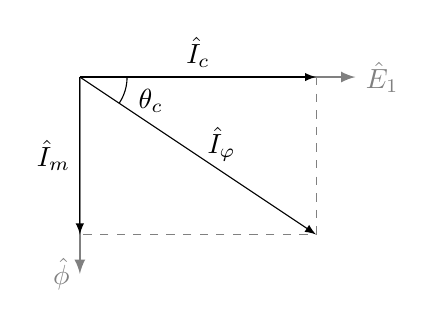
\begin{tikzpicture}
%grid
%\draw[gray,thick] (-2,-2) grid (2,2);
%\draw[help lines,xstep=0.1,ystep=0.1] (-2,-2) grid (2,2);
 \pgfmathsetmacro{\t}{0.3}  
\pgfmathsetmacro{\d}{0.9}  
\pgfmathsetmacro{\s}{0.05 cm} 
\draw[gray,thick,-latex](0,0)--(0,-2.5)node[left]{$\hat{\phi}$};
\draw[gray,thick,-latex](0,0)--(3.5,0)node[right]{$\hat{E}_1$};
\draw[-latex](0,0)--(3,0)node[above,pos=0.5]{$\hat{I}_c$};
\draw[-latex](0,0)--(0,-2)node[left,pos=0.5]{$\hat{I}_m$};
\draw[-latex](0,0)--(3,-2)node[above,pos=0.6]{$\hat{I}_\varphi$};
%
\draw[dashed,gray](3,0)--(3,-2)--(0,-2);
%angle
\begin{scope}
\clip (3,-2)--(0,0)--(3,0);
\draw (0,0) circle (0.6);
\end{scope}
\draw(0.9,-0.3)node {$\theta_c$};
\end{tikzpicture}
\caption{مختلف مرحلی سمتیوں کے زاویے۔}
\label{شکل_ٹرانسفارمر_مرکزی_ضیاع_اور_مقناطیسی_رو}
\end{figure}

غیر سائن نما ہیجان انگیز برقی رو \عددیء{i_{\varphi}} کو \اصطلاح{فوریئر} تسلسل\فرہنگ{فوریئر تسلسل}\حاشیہب{Fourier series}\فرہنگ{Fourier series} سے یوں لکھ سکتے ہیں۔
\begin{align} 
i_{\varphi}=\sum_n {\left( a_n \cos n \omega t + b_n \sin \omega t \right)}
\end{align}
اس میں \عددیء{(a_1 \cos \omega t+b_1 \sin \omega t)} کو \اصطلاح{بنیادی جزو}\فرہنگ{بنیادی جزو}\حاشیہب{fundamental component}\فرہنگ{fundamental component} کہتے ہیں اور باقی حصہ کو  \اصطلاح{موسیقائی جزو}\فرہنگ{موسیقائی جزو}\حاشیہب{harmonic components}\فرہنگ{harmonic components}  کہتے ہیں۔ بنیادی جزو میں \عددیء{a_1 \cos \omega t}، مقناطیسی بہاو سے وجود میں آنے والے امالی برقی دباو \عددیء{e_1} ،  جو کہ مساوات \حوالہ{مساوات_ٹڑانسفارمر_دباو_سمتیہ} میں دی گئی ہے کے ہم قدم ہے۔ یعنی  یہ دونوں وقت کے ساتھ یکساں بڑھتے اور گھٹتے ہیں جبکہ اس میں \عددیء{b_1 \sin \omega t} نوے درجہ زاویہ \عددیء{e_1}  کے پیچھے رہتا ہے۔ قالب میں مختلف وجوہات سے برقی طاقت کی ضائع  کو \عددیء{a_1 \cos \omega t} ظاہر  کرتی ہے۔اسی لئے اس جزو کو \اصطلاح{جزو قالبی ضیاع}\فرہنگ{قالبی ضیاع!جزو}\حاشیہب{core loss component}\فرہنگ{core loss component}  کہتے ہیں۔ہیجان انگیز برقی رو \عددیء{i_{\varphi}} سے اگر \عددیء{a_1 \cos \omega t} منفی کی جائے تو بقایا کو مقناطیس بنانے والا برقی رو\فرہنگ{مقناطیسی برقی رو} یا \اصطلاح{مقناطیسی برقی رو}\حاشیہب{magnetizing current}\فرہنگ{magnetizing current} کہتے ہیں۔ اس  کی تیسری موسیقائی جزو سب سے زیادہ اہم  ہے۔ قوی  ٹرانسفارمروں میں یہ تیسری موسیقائی جزو عموماً  کُل ہیجان انگیز برقی رو  کے \عددیء{40} فی صد ہوتی ہے۔  

سوائے وہاں، جہاں  ہیجان انگیز برقی رو کے اثرات پر غور کیا جا رہا ہو، ہم ہیجان انگیز برقی رو کے غیر سائن نما ہونے کو نظرانداز کرتے ہیں۔ قوی ٹرانسفارمر کی  ہیجان انگیز برقی رو اس کی کُل برقی رو\حاشیہد{کُل برقی رو سے مراد وہ برقی رو ہے جو کُل برقی بوجھ لادنے سے حاصل ہو} کے صرف \عددیء{5}  فی صد کے قریب ہوتی ہے۔ لہٰذا  اس کا اثر بہت کم ہوتا ہے۔ لہٰذا ہم  ہیجان انگیز برقی رو کو سائن نما تصور کر کے اس کے اثرات پر غور کرتے ہیں۔ایسا کرنے سے مسئلہ پر غور کرنا آسان ہو جاتا ہے۔ اس فرضی سائن نما  ہیجان انگیز برقی رو\حاشیہد{یعنی  بدلتی برقی رو \عددیء{i_{\varphi}} کو اب مرحلی سمتیہ کی مدد سے \عددیء{\hat{I_{\varphi}}} لکھتے ہیں} \عددیء{\hat{I_{\varphi}}}  کی موثر قیمت \عددیء{I_{\varphi,rms}} ، اصل  ہیجان انگیز برقی رو کی موثر قیمت کے برابر رکھی جاتی ہے جبکہ اس کا زاویہ \عددیء{\theta_c} یوں رکھا جاتا ہے کہ اس سے حاصل برقی ضیاع اصل برقی ضیاع کے برابر ہو۔ شکل \حوالہ{شکل_ٹرانسفارمر_مرکزی_ضیاع_اور_مقناطیسی_رو}  کی مدد سے یہ بات سمجھنی زیادہ آسان ہے۔ شکل میں اگر دیکھا جائے تو
\begin{align}
p_c=E_{rms} I_{\varphi,rms} \cos \theta_c
\end{align}
جہاں \عددیء{p_c} \اصطلاح{قالبی ضیاع}  ہے۔ لہٰذا  اگر \عددیء{\hat{I_{\varphi}}} اور \عددیء{\hat{E_1}} کے مابین \عددیء{\theta_c} کا زاویہ ہو تو اس سے قالبی ضیاع صحیح حاصل ہوتا ہے۔\عددیء{\hat{I_{\varphi}}} اسی زاویہ  سے  \عددیء{\hat{E_1}}  کے پیچھے رہتا ہے۔

\حصہ{تبادلہ برقی دباو اور تبادلہ برقی رو کے خصوصیات}
ہم شکل \حوالہ{شکل_ٹرانسفارمر_کامل_بار_بردار_ٹرانسفارمر}  کی مدد سے ٹرانسفارمر کا مطالعہ کرتے ہیں۔  ہم فرض کرتے ہیں کہ ابتدائی جانب لچھے کے \عددیء{N_1} اور ثانوی جانب لچھے کے \عددیء{N_2} چکر ہیں اور یہ کہ ان  دونوں لچھوں کی مزاحمت صفر ہے۔ ہم مزید یہ کہتے ہیں کہ پوری مقناطیسی بہاو  قالب ہی میں رہتا ہے اور دونوں لچھوں سے گزرتا ہے۔ قالب میں برقی توانائی ضائع نہیں ہوتی اور اس کی مقناطیسی مستقل اتنی زیادہ ہے کہ ہیجان انگیز برقی رو قابلِ نظر انداز ہے۔ برقی رو \عددیء{i_1}  اور \عددیء{i_2} کی سمتیں یوں رکھی گئی ہیں کہ ان سے وجود میں آنے والے مقناطیسی بہاو ایک دوسرے کی اُلٹ سمتوں میں  ہیں۔ اصل ٹرانسفارمر ان باتوں پر تقریباً پورے اترتے ہیں۔ ایسے ٹرانسفارمر کو کامل ٹرانسفارمر\فرہنگ{ٹرانسفارمر!کامل}\حاشیہب{ideal transformer}\فرہنگ{transformer!ideal}  کہتے ہیں۔
\begin{figure}
\centering
%\includegraphics{figTransformersLoadedIdealTransformer}
\begin{tikzpicture}
\def\height{2.5};
\def\width{2.5};
\def\thick{0.4};
\def\depthX{0.2};
\def\depthY{0.2};
\def\gap{0.05};
%grid
%\draw[gray,thick](0,0) grid (5,3);
%\draw[gray,thin,xstep=0.1,ystep=0.1](0,0) grid (5,3);
%going clockwise from origin
\draw(0,0)--++(0,\height)--++(\width,0)--++(0,-\height)--cycle;
\draw(0,0)++(\thick,\thick)--++(0,\height-2*\thick)--++(\width-2*\thick,0)--++(0,-\height+2*\thick)--cycle;
%
\draw(\thick,\thick)--++(\depthX,\depthY) --++(0,\height-2*\thick-\depthY);
\draw(\thick,\thick)--++(\depthX,\depthY) --++(\width-2*\thick-\depthX,0);
\draw(0,\height)--++(\depthX,\depthY)--++(\width,0)--++(-\depthX,-\depthY);
\draw(\width,0)--++(\depthX,\depthY)--++(0,\height)--++(-\depthX,-\depthY);

%left winding
\draw (0.6,1.9) to [out=45,in=0] (0.2,2);% to (-1.5,2);
\foreach \l in {1.9,1.7,1.5,1.3,1.1,0.9}{
\draw (0,\l) to [out=-135,in=45] (0.6,\l-0.2);
}
\draw (0,0.7) to (-1.5,0.7) to [american voltage source] (-1.5,2) to[short,i^=$i_1$] (0.2,2);   %input power
%right  winding
\draw (2.1,1.9) to [out=135,in=0] (2.4,2);% to (-1.5,2);
\foreach \l in {1.9,1.7,1.5,1.3,1.1,0.9}{
\draw (2.7,\l) to [out=-45,in=135] (2.1,\l-0.2);
}
\draw(2.4,2) to [short,i^={$i_2$}] ++(1.5,0) to [european resistor] ++(0,-1.3)--(2.7,0.7);

%flux
\draw[gray,-latex](0.5*\width,\height-0.5*\thick)--++(0.5*\width-0.5*\thick,0)--++(0,-\height+\thick)--++(-\width+\thick,0)--++(0,\height-\thick)
--++(0.5*\width-0.5*\thick,0);
\path[fill=white] (0.4*\width,0.1) rectangle (0.6*\width,0.3); %making roo for writing flux
\draw(0.5*\width,0.5*\thick)node{$_\varphi$};
%text
\draw (1,1.35)node{$N_1$};
\draw (-0.3,1.35)node{$v_1$};
\draw (-0.3,1.7)node{$+$};
\draw (-0.3,1)node{$-$};
\draw (1.7,1.35)node{$N_2$};
\draw (3,1.35)node{$v_2$};
\draw (3,1.7)node{$+$};
\draw (3,1)node{$-$};
\draw(4.2,1.5)node[right]{\RL{برقی بار}};
\end{tikzpicture}
\caption{کامل بوجھ بردار ٹرانسفارمر۔}
\label{شکل_ٹرانسفارمر_کامل_بار_بردار_ٹرانسفارمر}
\end{figure}

جب اس کامل ٹرانسفارمر کے ابتدائی لچھے پر بدلتی برقی دباو \عددیء{v_1} لاگو کیا جائے تو اس کے قالب میں بدلتا مقناطیسی بہاو  \عددیء{\varphi_m} وجود میں  آئے گا جو ابتدائی لچھے میں   لاگو برقی دباو \عددیء{v_1} کے برابر امالی برقی دباو \عددیء{e_1} کو جنم دے گا۔لہٰذا
\begin{align}
v_1=e_1=N_1 \frac{\dif \varphi_m}{\dif t}
\end{align}
یہ مقناطیسی بہاو دوسرے لچھے سے بھی گزرے گا اور اس میں \عددیء{e_2} امالی برقی دباو کو جنم دے گا جو ثانوی جانب کے سروں پر برقی دباو \عددیء{v_2}  کی صورت میں حاصل ہو گا۔ یعنی
\begin{align}
v_2=e_2=N_2 \frac{\dif \varphi_m}{\dif t}
\end{align}
ان دونوں کی نسبت سے
\begin{align}\label{مساوات_ٹرانسفارمر_تبادلہ_دباو}
\frac{v_1}{v_2}=\frac{N_1 \frac{\dif \varphi_m}{\dif t}}{N_2 \frac{\dif \varphi_m}{\dif t}}=\frac{N_1}{N_2}
\end{align}
لہٰذا ایک کامل ٹرانسفارمر دونوں لچھوں کے چکروں کی نسبت سے \اصطلاح{تبادلہ برقی دباو}\فرہنگ{برقی دباو!تبادلہ}\حاشیہب{voltage transformation}\فرہنگ{voltage!transformation} کرتا ہے۔

چونکہ یہ ایک کامل ٹرانسفارمر ہے لہٰذا اسے جتنی برقی طاقت ابتدائی جانب  دی جائے اتنی ہی برقی طاقت اس سے ثانوی جانب حاصل ہو گی،یعنی
\begin{align}
p=v_1 i_1 = v_2 i_2
\end{align}
یا
\begin{align}
\frac{v_1}{v_2}=\frac{i_2}{i_1}
\end{align}
مساوات  \حوالہ{مساوات_ٹرانسفارمر_تبادلہ_دباو} کی مدد سے
\begin{align}
\frac{v_1}{v_2}=\frac{i_2}{i_1}=\frac{N_1}{N_2}
\end{align}
یہ ایک انتہائی اہم نتیجہ ہے جو ٹرانسفارمر کی تبادلہ برقی دباو اور \اصطلاح{تبادلہ برقی رو}\فرہنگ{برقی رو!تبادلہ}\حاشیہب{current transformation}\فرہنگ{current!transformation}  کی خصوصیات بیان کرتا ہے۔اسے عموماً دو حصوں میں یوں لکھا جاتا ہے۔
\begin{gather}
\begin{aligned}\label{مساوات_ٹرانسفارمر_تبادلہ_دباو_رو}
\frac{v_1}{v_2}&=\frac{N_1}{N_2}\\
\frac{i_1}{i_2}&=\frac{N_2}{N_1}
\end{aligned}
\end{gather}
اس مساوات کی پہلی جزو کہتی ہے کہ ٹرانسفارمر کی دونوں جانب برقی دباو  ان کے چکروں کی راست متناسب  ہو گا جبکہ مساوات کی دوسری جزو کہتی ہے کہ ٹرانسفارمر کے دونوں جانب برقی رو ان کے چکروں کے بالعکس متناسب ہو گا۔

\ابتدا{مثال}
	شکل  \حوالہ{شکل_ٹرانسفارمر_کامل_بار_بردار_ٹرانسفارمر}  میں اگر
\begin{align*}
\hat{V_1}&=220 \phase{0}\\
N_1:N_2&=220:22\\
Z&=R=\SI{10}{\ohm}
\end{align*}
ہوں تو ٹرانسفارمر کی دونوں جانب برقی دباو اور برقی رو معلوم کریں۔

حل:
ابتدائی جانب برقی دباو دیا گیا ہے یعنی \عددیء{220} وولٹ جبکہ ثانوی جانب برقی دباو مساوات \حوالہ{مساوات_ٹرانسفارمر_تبادلہ_دباو_رو} کی پہلی جزو کی مدد سے حاصل کیا جاتا ہے یعنی
\begin{align*}
\hat{V_2}=\frac{N_2}{N_1} \hat{V_1}=\frac{22}{220} \times 220\phase {0}=22\phase{0}
\end{align*}
ثانوی جانب \عددیء{22} وولٹ ہیں جو ابتدائی جانب برقی دباو کے ہم قدم ہے۔ثانوی جانب یہ برقی دباو \عددیء{10} اوہم کی مزاحمت میں برقی رو پیدا کرے گا جسے اوہم کے قانون سے حاصل کیا جاتا ہے یعنی
\begin{align*}
\hat{I_2}=\frac{22 \phase {0}}{10}=2.2\phase {0}
\end{align*}
ثانوی جانب \عددیء{2.2} ایمپیئر برقی رو ہے۔ ابتدائی جانب کی برقی رو مساوات \حوالہ{مساوات_ٹرانسفارمر_تبادلہ_دباو_رو} کی دوسری جزو کی مدد سے حاصل کی جاتی ہے یعنی
\begin{align*}
\hat{I_1}=\frac{N_2}{N_1} \hat{I_2}=\frac{22}{220} \times 2.2\phase{0}=0.22\phase{0}
\end{align*}
\انتہا{مثال}

اس مثال کے نتائج ایک جگہ لکھ کر ان پر غور کرتے ہیں۔
\begin{align*}
\hat{V_1}=220\phase{0}, \quad \hat{V_2}=22\phase{0}, \quad \hat{I_1}=0.22\phase{0}, \quad \hat{I_2}=2.2\phase{0}
\end{align*}
ہم دیکھتے ہیں ابتدائی جانب برقی دباو ثانوی جانب کی برقی دباو کے دس گنا ہے جبکہ برقی رو میں قصہ اُلٹ ہے۔ثانوی جانب کی برقی رو ابتدائی جانب کی برقی رو کے دس گنا ہے۔طاقت دونوں جانب برابر ہے۔یہ نہایت اہم ہے کہ آپ اس بات کو اچھی طرح سمجھ لیں کہ جس جانب برقی دباو زیادہ ہوتا ہے اس جانب برقی رو کم ہوتی ہے۔ لہٰذا زیادہ برقی دباو کی جانب لچھے کے چکر زیادہ ہوں گے اور اس لچھے میں نسبتاً باریک برقی تار استعمال ہو گی جبکہ کم برقی دباو کا لچھا کم چکر کا ہو گا اور اس میں نسبتاً موٹی برقی تار استعمال ہو گی۔ 

\ابتدا{مثال}
	صفحہ \حوالہصفحہ{شکل_ٹرانسفارمر_رکاوٹ_کا_تبادلہ} پر دکھائے گئے شکل \حوالہ{شکل_ٹرانسفارمر_رکاوٹ_کا_تبادلہ}-الف سے رجوع کریں۔ اس شکل میں رکاوٹ \عددیء{Z_2} کو  بدلتی برقی دباو \عددیء{\hat{V_1}} کے ساتھ ایک ٹرانسفارمر کے ذریعہ جوڑا گیا ہے۔اگر
\begin{align*}
\hat{V_1}=110\phase{0},\quad Z_2=R+j X=3+j 2,\quad N_1:N_2=220:22 
\end{align*}
ہوں تو رکاوٹ میں برقی رو اور طاقت کا ضیاع معلوم کریں۔

حل:
	ٹرانسفارمر کی تبادلہ برقی دباو کی خصوصیت سے اس کے ابتدائی جانب \عددیء{110} وولٹ برقی دباو ٹرانسفارمر کی ثانوی جانب تبدیل ہو کر  \عددیء{\hat{V_s}} ہو جائیں گے جہاں
\begin{align*}
\hat{V_s}=\frac{N_2}{N_1} \hat{V_1}=\frac{22}{220} \times 110\phase{0}=11\phase{0}
\end{align*}
ہے لہٰذا
\begin{align*}
\hat{I_2}=\frac{\hat{V_s}}{Z}=\frac{11\phase{0}}{3+j 2}= 3.05\phase{-33.69\degree}
\end{align*}
اور برقی طاقت کا ضیاع \عددیء{p_z}
\begin{align*}
p_z=I_2^2 R=3.05^2 \times 3=\SI{27.9}{\watt}
\end{align*}
\انتہا{مثال}

\حصہ{ثانوی جانب بوجھ کا ابتدائی جانب اثر}\شناخت{حصہ_ٹرانسفارمر_ثانوی_بار_کا_ابتدائی_جانب_اثر}
یہاں صفحہ \حوالہصفحہ{شکل_ٹرانسفارمر_کامل_بار_بردار_ٹرانسفارمر} پر دکھائے گئے  شکل \حوالہ{شکل_ٹرانسفارمر_کامل_بار_بردار_ٹرانسفارمر}  سے رجوع کریں۔ہم حصہ \حوالہ{حصہ_ٹرانسفارمر_امالی_برقی_دباو}  میں دیکھ چکے ہیں کہ اگر ایک بے بوجھ ٹرانسفارمر کی ابتدائی لچھے پر بدلتی برقی دباو \عددیء{v_1} لاگو کی جائے تو اس لچھے میں ہیجان انگیز برقی رو \عددیء{i_{\varphi}} گزرے گی۔اس برقی رو کی مقناطیسی دباو \عددیء{N_1 i_{\varphi}} قالب میں مقناطیسی بہاو \عددیء{\varphi_m}\حاشیہد{\عددیء{\varphi} کو یہاں \عددیء{\varphi_m} کہا گیا ہے۔} کو جنم دے گی ۔اگر لچھے کی مزاحمت صفر ہو تو \عددیء{\varphi_m} ابتدائی لچھے میں \عددیء{e_1} امالی برقی دباو پیدا کرے گی جہاں
\begin{align}\label{مساوات_ٹرانسفارمر_دباو_برابر_بہاو_تفرق}
v_1=e_1=N_1 \frac{\dif \varphi_m}{\dif t}
\end{align}
ہو گی۔

اب ہم ثانوی جانب  برقی بوجھ لادتے ہیں۔ ایسا کرنے سے بوجھ بردار ٹرانسفارمر\فرہنگ{ٹرانسفارمر!بوجھ بردار}\حاشیہب{loaded transformer}  کے  ثانوی جانب  برقی رو \عددیء{i_2} رواں ہو گی جس کی وجہ سے \عددیء{N_2 i_2} مقناطیسی دباو وجود میں آئے گی۔ اس مقناطیسی دباو کی وجہ سے قالب میں مقناطیسی بہاو \عددیء{\varphi_{\textup{بوجھ}}}  پیدا ہو گا۔ اگر اس مقناطیسی بہاو کا کچھ  نہ کیا جائے تو قالب میں پہلے سے موجود مقناطیسی بہاو تبدیل ہو کر \عددیء{\varphi_{\textup{نئی}}=\varphi_{m}-\varphi_{\textup{بوجھ}}} ہو جائے گا اور یوں ابتدائی لچھے میں امالی دباو تبدیل ہو کر \عددیء{e_{\textup{نئی}}} ہو جائے گا۔  لہٰذا ابتدائی جانب پر اب امالی دباو اور اس پر لاگو برقی دباو برابر نہیں ہونگے جو کہ مساوات \حوالہ{مساوات_ٹرانسفارمر_دباو_برابر_بہاو_تفرق}  کی موجودگی میں ناممکن ہے۔ لہٰذا اس مقناطیسی بہاو \عددیء{\varphi_{\textup{بوجھ}}}  کے اثر کو ختم کرنے کیلئے ابتدائی لچھے میں برقی رو \عددیء{i_{1}} نمودار ہو گی جو اس مقناطیسی دباو یعنی \عددیء{N_2 i_2} کے اثر کو ختم کر دے گی یعنی
\begin{align}
N_1 i_1=N_2 i_2
\end{align}
یہ وہ ذریعہ ہے جس سے ابتدائی جانب معلوم ہوتا ہے کہ ثانوی جانب پر بوجھ لدا ہے۔ شکل میں دونوں لچھوں میں برقی رو کی سمتیں یوں ہیں کہ ان کے مقناطیسی بہاو آپس میں اُلٹ سمت میں ہیں لہٰذا  قالب میں اب پھر مقناطیسی بہاو \عددیء{\varphi_m}  کے برابر  ہے جیسا کہ ہونا چاہئے تھا۔ اس مساوات کو یوں لکھ سکتے ہیں
\begin{align}\label{مساوات_ٹرانسفارمر_برقی_رو_اور_چکر_شرح}
\frac{i_1}{i_2}=\frac{N_2}{N_1}
\end{align}
یہ وہی مساوات ہے جو کامل ٹرانسفارمر کے لئے ثابت کی گئی تھی۔
%
\حصہ{ٹرانسفارمر کی علامت پر نقطوں کا مطلب}
	شکل \حوالہ{شکل_ٹرانسفارمر_کامل_بار_بردار_ٹرانسفارمر}  میں ٹرانسفارمر کے لچھوں پر نکتے لگائے گئے ہیں۔ یہ نکتے اس بات کو ظاہر کرتے ہیں کہ اگر ایک طرف کے لچھے پر برقی دباو \عددیء{v_1} یوں ہو کہ نکتے والا سرا مثبت اور بغیر نکتے والا سرا منفی ہو تو دوسرے لچھے  پر برقی دباو \عددیء{v_2} اس طرح ہو گا کہ اس لچھے کا بھی  نکتے والا سرا مثبت اور بغیر نکتے والا سرا منفی ہو گا۔

مزید یہ کہ ابتدائی جانب برقی رو ٹرانسفارمر کے نکتے والے سرے سے ٹرانسفارمر کی اندر جانب ہو گا جبکہ ثانوی جانب برقی رو نقطہ والے سرے سے ٹرانسفارمر سے باہر نکلے گا۔

 یوں  \عددیء{v_1} اور \عددیء{v_2} وقت کے ساتھ یکساں تبدیل ہوتے ہیں اور ان کے مابین صفر زاویہ ہے۔ لہٰذا یہ دو برقی دباو \اصطلاح{ہم قدم}\فرہنگ{ہم قدم}\حاشیہب{in-phase}\فرہنگ{in-phase} ہیں۔

\حصہ{رکاوٹ کا تبادلہ}
اس حصہ میں کامل ٹرانسفارمر میں رکاوٹ کے تبادلہ پر غور کیا جائے گا۔شکل \حوالہ{شکل_ٹرانسفارمر_رکاوٹ_کا_تبادلہ}-الف میں ایک ٹرانسفارمر دکھایا گیا ہے جس کی ابتدائی جانب سائن نما برقی دباو  \عددیء{\hat{V_1}=V_1\phase{\theta}}  لاگو کیا گیا ہے۔یہاں مرحلی سمتیہ استعمال کئے جائیں گے۔

جیسے اُوپر ذِکر ہوا، برقی دباو \عددیء{\hat{V_1}} اور \عددیء{\hat{V_2}} آپس میں ہم قدم ہیں اور  اسی طرح برقی رو \عددیء{\hat{I_1}} اور \عددیء{\hat{I_2}} آپس میں  ہم قدم ہیں۔مساوات \حوالہ{مساوات_ٹرانسفارمر_تبادلہ_دباو} اور  مساوات \حوالہ{مساوات_ٹرانسفارمر_برقی_رو_اور_چکر_شرح}   کو مرحلی سمتیہ کی مدد سے یوں لکھ سکتے ہیں
\begin{gather}
\begin{aligned}
\hat{V_1}&=\left(\frac{N_1}{N_2} \right) \hat{V_2}\\
\hat{I_1}&=\left(\frac{N_2}{N_1} \right) \hat{I_2}
\end{aligned}
\end{gather}
چونکہ رکاوٹ
\begin{align}
Z_2=\frac{\hat{V_2}}{\hat{I_2}}=\abs{Z_2}\phase{\theta_z}
\end{align}
کے برابر ہے لہٰذا
\begin{align}\label{مساوات_ٹرانسفارمر_تبادلہ_رکاوٹ_الف}
\frac{\hat{V_1}}{\hat{I_1}}=\left(\frac{N_1}{N_2} \right)^2 \frac{\hat{V_2}}{\hat{I_2}}=\left(\frac{N_1}{N_2} \right)^2  Z_2
\end{align}
اب اگر ہم ٹرانسفارمر بمع اس پر لدے رکاوٹ  کی جگہ برقی دباو \عددیء{\hat{V_1}} کو رکاوٹ \عددیء{Z_1} پر لاگو کریں جہاں اس رکاوٹ کی قیمت
\begin{align}\label{مساوات_ٹرانسفارمر_متبادل_رکاوٹ_تعریف}
Z_1=\left(\frac{N_1}{N_2} \right)^2  Z_2
\end{align}
ہو تو \عددیء{\hat{V_1}} سے حاصل برقی رو یا اس سے حاصل برقی طاقت تبدیل نہیں ہو گی۔یہ شکل \حوالہ{شکل_ٹرانسفارمر_رکاوٹ_کا_تبادلہ}-ب میں دکھایا گیا ہے جہاں سے واضح ہے کہ
\begin{align}\label{مساوات_ٹرانسفارمر_تبادلہ_رکاوٹ_ب}
\frac{\hat{V_1}}{\hat{I_1}}=Z_1=\left(\frac{N_1}{N_2} \right)^2  Z_2
\end{align}
لہٰذا شکل کے الف اور ب دونوں حصوں سے  برقی دباو \عددیء{\hat{V_1}} کی برقی رو مساوات \حوالہ{مساوات_ٹرانسفارمر_تبادلہ_رکاوٹ_الف}  اور مساوات \حوالہ{مساوات_ٹرانسفارمر_تبادلہ_رکاوٹ_ب}  سے یکساں حاصل ہوتی ہے یعنی
\begin{align}
\hat{I_1}=\frac{\hat{V_1}}{\left(\frac{N_1}{N_2} \right)^2  Z_2}
\end{align}
اور یوں الف اور با  دونوں حصوں میں  برقی دباو \عددیء{\hat{V_1}} سے حاصل برقی طاقت برابر ہے یعنی
\begin{align}
p=\hat{V_1} \cdot \hat{I_1}=\frac{V_1^2 \cos \theta_z}{\left(\frac{N_1}{N_2} \right)^2  \abs{Z_2}}
\end{align}
%
\begin{figure}
\centering
%\includegraphics{figTransformersImpedanceTransformation}
\begin{tikzpicture}
%grid
%\draw[gray,thick] (-3,-3) grid (3,3);
%\draw[gray,thin,xstep=0.1,ystep=0.1] (-3,-3) grid (3,3);
%transformer outer dimensions
\pgfmathsetmacro{\h}{2.5}
\begin{scope}[xshift=1.5cm,yshift=5cm]
\draw (0,0) node [transformer] (T1){};
\draw (T1.base)node[above] {$N_1:N_2$};
\draw(T1.A2) to [short] ++(-2,0) to [american voltage source,l=$\hat{V}_1$] ++(0,2.1) to  [short,i^=$\hat{I}_1$]  (T1.A1);
\draw(T1.B1) to [short,i^=$\hat{I}_2$] ++(2,0) to [european resistor,l=$Z_2$] ++(0,-2.1) to (T1.B2);
%text
\draw(2.5,-1) node{$
\begin{aligned}
&+\\
&\hat{V}_2\\
&-
\end{aligned}
$};
%urdu
\draw (4,-2.1) node {الف};
\end{scope}
%
\draw (0,0) to [american voltage source,l=$\hat{V}_1$] ++(0,2.1) to [short,i_=$\hat{I}_1$] ++(3,0) to [european resistor,l=${Z'=\left(\frac{N_1}{N_2} \right)^2 Z_2}$] ++(0,-2.1) to (0,0);
%urdu
\draw (5.5,0) node {ب};
\end{tikzpicture}
\caption{ٹرانسفارمر کی خاصیت تبادلہ رکاوٹ۔}
\label{شکل_ٹرانسفارمر_رکاوٹ_کا_تبادلہ}
\end{figure}
	یوں اگر ٹرانسفارمر کے ثانوی جانب  رکاوٹ \عددیء{Z_2} کا بوجھ ہو تو حساب کرتے وقت ہم یہ اخذ کر سکتے ہیں کہ  ٹرانسفارمر بمع رکاوٹ \عددیء{Z_2} کی  جگہ  صرف  \عددیء{Z_1} رکاوٹ لگی ہے، جہاں \عددیء{Z_1} مساوات \حوالہ{مساوات_ٹرانسفارمر_متبادل_رکاوٹ_تعریف}  سے حاصل ہوتی ہے۔ رکاوٹ کا یوں ٹرانسفارمر کی ایک جانب سے دوسری جانب تبادلہ کیا جاسکتا ہے۔ٹرانسفارمر کی اس خاصیت کو  \اصطلاح{تبادلہ رکاوٹ}\فرہنگ{تبادلہ!رکاوٹ}\حاشیہب{impedance transformation}\فرہنگ{impedance transformation} کی خصوصیت  کہتے ہیں۔
%
\ابتدا{مثال}
شکل \حوالہ{شکل_ٹرانسفارمر_برقی_طاقت_کی_منتقلی}-الف میں رکاوٹ \عددیء{Z_B} کا برقی بوجھ ایک جنریٹر پر لدا ہے۔بوجھ تک برقی طاقت دو برقی تاروں کے ذریعہ منتقل کیا گیا ہے۔ان تاروں کی مجموعہ رکاوٹ \عددیء{Z_t} ہے۔
\begin{figure}
\centering
%\includegraphics{figTransformersPowerTransmission}
\begin{tikzpicture}
%grid
%\draw[gray,thick](-3,-3) grid (7,3);
%\draw[gray,thin,xstep=0.1,ystep=0.1](-3,-3) grid (7,3);
%
\begin{scope}[yshift=2cm]
%going clockwise from origin
\draw(0,0) to [american voltage source,l=$\hat{V}$] (0,2) to [short,i^=$\hat{I}_t$] ++(1,0) to [resistor,l=$\SI{0.1}{\ohm}$] ++(2.5,0) to [inductor,l=$j\SI{0.15}{\ohm}$] ++(2.5,0) to [european resistor,l=${Z_B=2+j4}$] ++(0,-2) to [short] (0,0);
%text
\draw(5.4,1) node{$
\begin{aligned}
&+\\
&V_B\\
&-
\end{aligned}
$};
\end{scope}
%
\draw (0,0) node [transformer core](T1){}  % reminded by @PaulGessler, thanks.
 %     (T1.A1) node[above] {A1}
   %   (T1.A2) node[below] {A2}
     % (T1.B1) node[above] {B1} 
    %  (T1.B2) node[below] {B2}
      (T1.base) node[above]{$
\begin{aligned}
1&:10\\
N_1&:N_2
\end{aligned}
$};
\draw (6,0) node [transformer core](T2){}  % reminded by @PaulGessler, thanks.
 %     (T2.A1) node[above] {A1}
   %   (T2.A2) node[below] {A2}
     % (T2.B1) node[above] {B1} 
    %  (T2.B2) node[below] {B2}
      (T2.base) node[above]{$
\begin{aligned}
10&:1\\
N_3&:N_4
\end{aligned}
$};
%going clockwise from origin
\draw (T1.B1) to [short,i_=$\hat{I}_t$] ++(0.5,0) to [resistor,l=$\SI{0.1}{\ohm}$] ++(1.5,0) to [inductor,l=$j\SI{0.15}{\ohm}$] (T2.A1) ;
\draw(T1.B2) to (T2.A2);
%
\draw(T1.A2)--++(-1,0) to [american voltage source,l=$\hat{V}$] ++(0,2.1) [short,i_=$\hat{I}_G$] to (T1.A1);
%
\draw(T2.B1) to [short,i_=$\hat{I}_B$] ++(1,0) to [european resistor,l=$Z_B$] ++(0,-2.1) to (T2.B2);
\draw(0,-2.5) node{$T1$};
\draw(6,-2.5) node{$T2$};
\end{tikzpicture}
\caption{برقی طاقت کی منتقلی۔}
\label{شکل_ٹرانسفارمر_برقی_طاقت_کی_منتقلی}
\end{figure}
%
\begin{figure}
\centering
%\includegraphics{figTransformersStepByStepSolution}
\begin{tikzpicture}
%grid
%\draw[gray,thick] (-3,-3) grid (7,3);
%\draw[gray,thin,xstep=0.1,ystep=0.1] (-3,-3) grid (7,3);
%transformer outer dimensions
\pgfmathsetmacro{\h}{2.5}
\begin{scope}[xshift=0cm,yshift=3cm]
\draw (0,0) node [transformer] (T1){};
\draw (T1.base)node[above] {$1:10$};
\draw(T1.A2) to [short] ++(-2,0) to [american voltage source,l=$\hat{V}_1$] ++(0,2.1) to  [short,i^=$\hat{I}_G$]  (T1.A1);
\draw(T1.B1) to  [short,i>=$\hat{I}_t$] ++(0.5,0) to [european resistor,l=$\SI{0.1}{\ohm}$] ++(2,0) to [inductor,l=$j\SI{0.15}{\ohm}$] ++(2,0) to [european resistor,l=${Z_B'=200+j 400}$] ++(0,-2.1) to (T1.B2);
%urdu
\draw (7,-2.1) node {الف};
\end{scope}
%
\begin{scope}[xshift=3.5cm,yshift=0cm]
\draw (0,0) node [transformer] (T1){};
\draw (T1.base)node[above] {$1:10$};
\draw(T1.A2) to [short] ++(-1,0) to [american voltage source,l=$\hat{V}_1$] ++(0,2.1) to  [short,i^=$\hat{I}_G$]  (T1.A1);
\draw(T1.B1) to  [short,i>=$\hat{I}_t$]++(1,0) to [european resistor,l=${Z'=200.1+j400.15}$] ++(0,-2.1) to (T1.B2);
%urdu
\draw (3.5,-2.1) node {ب};
\end{scope}
%
\begin{scope}[xshift=-3cm,yshift=-2.1cm]
\draw(0,0)  to [american voltage source,l=$\hat{V}_1$] ++(0,2.1) to  [short,i^=$\hat{I}_G$]  ++(1.5,0) to [european resistor,l=$Z''$] ++(0,-2.1) to [short] (0,0);
%urdu
\draw (2,0) node {پ};
\end{scope}
\end{tikzpicture}
\caption{ٹرانسفارمر قدم با قدم حل کرنے کا طریقہ۔}
\label{شکل_ٹرانسفارمر_قدم_با_قدم_حل}
\end{figure}

شکل-ب میں جنریٹر کے قریب نسب برقی دباو بڑھانے والا ٹرانسفارمر برقی دباو کو دس گنا بڑھاتا ہے اور برقی بوجھ کے قریب نسب برقی دباو گھٹانے والا ٹرانسفارمر برقی دباو کو دس گنا گھٹاتا ہے۔اس حصہ میں وہی برقی تار استعمال کئے گئے ہیں لہٰذا ان کی بھی مجموعہ رکاوٹ \عددیء{Z_t} ہی ہے۔
اگر 
\begin{align*}
Z_B=2+j 4, \quad Z_t=0.1 +j 0.15, \quad \hat{V}=415\phase{0}
\end{align*}
ہوں تو دونوں صورتوں میں
\begin{itemize}
\item
برقی بوجھ پر برقی دباو معلوم کریں،
\item
برقی تاروں میں برقی طاقت کی ضیاع معلوم کرین۔
\end{itemize}

حل الف:
\begin{align*}
\hat{I_G}=\hat{I_t}=\hat{I_B}&=\frac{\hat{V}}{Z_t+Z_B}=\frac{415\phase{0}}{0.1+j 0.15+2+j 4}\\
&=\frac{415\phase{0}}{2.1+j 4.15}=89.23\phase{-63.159\degree}\\
&=40.3-j79.6
\end{align*}
یوں رکاوٹ پر برقی دباو
\begin{align*}
\hat{V_B}=\hat{I_B} Z_B&=\left(40.3-j79.6 \right) \left( 2+j 4\right)\\
&=399+j2=399\phase{0.287\degree}
\end{align*}
اور برقی تاروں میں برقی طاقت کا ضیاع ہے
\begin{align*}
p_t=I_t^2 R_t=89.23^2 \times 0.1=\SI{796}{\watt}
\end{align*}

حل ب:
شکل \حوالہ{شکل_ٹرانسفارمر_برقی_طاقت_کی_منتقلی} اور شکل \حوالہ{شکل_ٹرانسفارمر_قدم_با_قدم_حل}  سے رجوع کریں۔شکل  \حوالہ{شکل_ٹرانسفارمر_برقی_طاقت_کی_منتقلی} میں ٹرانسفارمر \عددیء{T_2} کے ثانوی جانب رکاوٹ کا مساوات \حوالہ{مساوات_ٹرانسفارمر_متبادل_رکاوٹ_تعریف}  کی مدد سے اس کی ابتدائی جانب تبادلہ سے ملتا ہے
\begin{align*}
Z_B'=Z_1=\left(\frac{N_3}{N_4} \right)^2 Z_B=\left(\frac{10}{1} \right)^2 \left(2+j 4 \right)=200+j 400
\end{align*}
یوں شکل \حوالہ{شکل_ٹرانسفارمر_قدم_با_قدم_حل}-الف حاصل ہوتا ہے۔اس شکل میں اب برقی تار کی رکاوٹ اور  تبادلہ شدہ رکاوٹ سلسلہ وار جُڑے ہیں۔ان کے مجموعہ  کو \عددیء{Z'} کہتے ہوئے
\begin{align*}
Z'=Z_t+Z_B'=0.1+j 0.15+200+j 400=200.1+j400.15
\end{align*}
یہ شکل \حوالہ{شکل_ٹرانسفارمر_قدم_با_قدم_حل}-ب میں دکھایا گیا ہے۔ایک مرتبہ دوبارہ مساوات \حوالہ{مساوات_ٹرانسفارمر_متبادل_رکاوٹ_تعریف}  استعمال کرتے ہوئے
\begin{align*}
Z''=\left(\frac{N_1}{N_2} \right)^2 Z'=\left(\frac{1}{10} \right)^2 \left(200.1+j400.15 \right)=2.001+j4.0015
\end{align*}
شکل \حوالہ{شکل_ٹرانسفارمر_قدم_با_قدم_حل}-پ میں دکھایا گیا ہے۔اب
\begin{align*}
\hat{I_G}=\frac{\hat{V}}{Z''}=\frac{415\phase{0}}{2.001+j4.0015}=92.76\phase{-63.432\degree}
\end{align*}
یہاں سے شکل \حوالہ{شکل_ٹرانسفارمر_قدم_با_قدم_حل}-ب  کی مدد سے اگر جنریٹر کی برقی رو معلوم ہو تو تبادلہ برقی رو سے
\begin{align*}
\hat{I_t}=\left(\frac{N_1}{N_2} \right) \hat{I_G}=\left(\frac{1}{10}\right) 92.76\phase{-63.432\degree}=9.276\phase{-63.432\degree}
\end{align*}
اس سے برقی تار میں طاقت کا ضیاع
\begin{align*}
p_t=I_t^2 R_t=9.276^2  \times 0.1=\SI{8.6}{\watt}
\end{align*}
اسی طرح شکل \حوالہ{شکل_ٹرانسفارمر_برقی_طاقت_کی_منتقلی}  میں اگر \عددیء{\hat{I_t}} معلوم ہو تو تبادلہ برقی رو سے
\begin{align*}
\hat{I_B}&=\left(\frac{N_3}{N_4}\right) \hat{I_t}=\left(\frac{10}{1}\right) 9.276\phase{-63.432\degree}\\
&=92.76\phase{-63.432\degree}=41.5-j 82.9
\end{align*}
اور رکاوٹ پر برقی دباو
\begin{align*}
\hat{V_B}=\hat{I_B} Z_B=\left(41.5-j 82.9 \right) \left(2+j 4 \right)=414+j 0.2
\end{align*}
ہو گی۔

ٹرانسفارمر کے بغیر برقی طاقت کی منتقلی میں برقی تاروں میں طاقت کی ضیاع \عددیء{796} واٹ ہے جبکہ ٹرانسفارمر کے استعمال سے یہ صرف \عددیء{8.6} واٹ ہے یعنی \عددیء{92} گنا کم۔یہی ٹرانسفارمر کی نہایت مقبولیت کی وجہ ہے۔ 
\انتہا{مثال}
%
\حصہ{ٹرانسفارمر کے وولٹ-ایمپیئر}
ٹرانسفارمر کی دونوں جانب برقی دباو ان لچھوں کے چکر پر منحصر ہوتا ہے۔ٹرانسفارمر ایک خاص برقی دباو اور برقی رو کے لئے بنائے جاتے ہیں۔ٹرانسفارمر جس برقی دباو \عددیء{V_1:V_2} کے لئے بنائے جائیں یہ اس سے کم برقی دباو پر بھی استعمال کئے جا سکتے ہیں اگرچہ یہ عموماً بنائے گئے برقی دباو پر ہی چلائے جاتے ہیں۔اسی طرح ٹرانسفارمر جتنی برقی رو \عددیء{I_1:I_2} کے لئے بنائے جائیں انہیں اس سے کم برقی رو پر استعمال کیا جا سکتا ہے۔حقیقت میں عموماً ٹرانسفارمر سے حاصل برقی رو اس حد سے کم ہی رکھی جاتی ہے۔

ٹرانسفارمر کی ایک جانب کی برقی دباو اور برقی رو کا حاصل ضرب اس کی دوسری جانب کی برقی دباو اور برقی رو کے حاصل ضرب کے برابر ہوتا ہے یعنی
\begin{align}
V_1 I_1=V_2 I_2
\end{align}
برقی دباو اور برقی رو کے حاصلِ ضرب  یعنی \عددیء{V_1 I_1} یا \عددیء{V_2 I_2} کو ٹرانسفارمر کی وولٹ ضربِ ایمپیئر کہتے ہیں جسے عموماً چھوٹا کر کے صرف \اصطلاح{وولٹ-ایمپیئر}\فرہنگ{وولٹ-ایمپیئر}
\حاشیہب{volt-ampere, VA}\فرہنگ{volt-ampere}\فرہنگ{VA}  کہا جاتا ہے\حاشیہد{وولٹ-ایمپیئر کو عموماً کلو وولٹ-ایمپیئر یعنی \عددیء{\si{\kilo \volt \ampere}} میں بیان کیا جاتا ہے}۔یہ ٹرانسفارمر کی برقی سکت کی ناپ ہے جو اس پر لگی تختی پر لکھا جاتا ہے۔اس تختی پر ٹرانسفارمر کے برقی دباو اور برقی تعداد ارتعاش بھی لکھے جاتے ہیں۔یوں ٹرانسفارمر کے وولٹ-ایمپیئر
\begin{align}\label{مساوات_ٹرانسفارمر_وولٹ_ایمپئیر}
\textup{\RL{وولٹ-ایمپیئر}}= V_1 I_1 = V_2 I_2
\end{align}
ہوں گے۔

اگرچہ یہاں ذکر ٹرانسفارمر کا ہو رہا ہے دراصل برقی مشین یعنی موٹر اور جنریٹر کی تختیوں پر بھی ان کے چالو حالت کے برقی دباو، ان کے وولٹ-ایمپیئر اور برقی تعداد ارتعاش لکھے جاتے ہیں۔اس کی وجہ یہ ہے کہ ان سب مشین کی کارکردگی کے بنیادی اصول ایک ہی طرح کے ہیں۔

\ابتدا{مثال}
ایک \عددیء{25000 } وولٹ-ایمپیئر اور \عددیء{11000:220} وولٹ برقی سکت  کے ٹرانسفارمر کے زیادہ برقی دباو کی جانب \عددیء{11000} وولٹ لاگو ہیں۔
\begin{itemize}
\item
اس کی ثانوی جانب زیادہ سے زیادہ کتنی برقی بوجھ ڈالی جا سکتی ہے۔
\item
اس زیادہ سے زیادہ برقی بوجھ پر اس کے ابتدائی لچھے میں برقی رو حاصل کریں۔
\end{itemize}

حل:	اس ٹرانسفارمر کی معلومات یہ ہیں
\begin{align*}
\SI{25}{\kilo \volt \ampere}, \quad 11000:220\,\textup{V}
\end{align*}
اس کی ثانوی جانب برقی دباو تبادلہ برقی دباو کی مساوات سے  \عددیء{220 } وولٹ حاصل ہوتا ہے۔یوں اس کی ثانوی جانب یعنی کم برقی دباو کی جانب زیادہ سے زیادہ برقی رو مساوات \حوالہ{مساوات_ٹرانسفارمر_وولٹ_ایمپئیر}  سے حاصل کیا جاتا ہے۔
\begin{align*}
I_2=\frac{25000}{220}=\SI{113.636}{\ampere}
\end{align*}
اسی طرح اس کی ابتدائی جانب زیادہ سے زیادہ برقی رو اسی مساوات سے یوں حاصل ہوتی ہے
\begin{align*}
I_1=\frac{25000}{11000}=\SI{2.27}{\ampere}
\end{align*}
\انتہا{مثال}
%
ٹرانسفارمر کی دونوں جانب لچھوں میں استعمال برقی تار کی موٹائی یوں رکھی جاتی ہے کہ ان میں کثافتِ برقی رو \عددیء{J}\حاشیہد{\عددیء{\SI{1000}{\kilo \volt \ampere}}  ٹرانسفارمر کی لچھوں میں کثافتِ برقی رو تقریباً  \عددیء{\SI{3}{\ampere / \milli \meter \squared}} رکھی جاتی ہے} یکساں ہو۔لچھوں کی مزاحمت میں برقی رو گزرنے سے برقی طاقت کا ضیاع ہوتا ہے جس سے یہ گرم ہوتے ہیں۔ٹرانسفارمر کی برقی رو کی حد لچھوں کی گرمائش پر منحصر ہوتی ہے۔ان کی زیادہ سے زیادہ حرارت کو محفوظ حد کے اندر رکھا جاتا ہے۔

بڑے ٹرانسفارمر کے قالب اور لچھے ایک غیر موصل تیل سے بھری ٹینکی میں ڈبوئے رکھے جاتے ہیں۔یہ تیل ایک تو برقی لچھوں کی حرارت کم کرنے میں مدد دیتا ہے اور دوسری جانب غیر موصل ہونے کی وجہ سے یہ زیادہ برقی دباو کے حصوں کو برقی طور پر جدا رکھنے میں مدد دیتا ہے۔یہ تیل تقریباً  \عددیء{\SI{80}{\celsius}} پر خراب ہونا شروع ہو جاتا ہے اور ہر \عددیء{\SI{8}{\celsius}} اضافی درجہ حرارت پر اس کی زندگی آدھی ہوتی رہتی ہے۔یعنی اگر \عددیء{\SI{80}{\celsius}} پر تیل کی کارآمد زندگی \عددیء{x} سال ہے تو \عددیء{\SI{88}{\celsius}} پر \عددیء{x/2} سال اور  \عددیء{\SI{96}{\celsius}} پر یہ صرف  \عددیء{x/4} سال ہو گی۔

	ٹرانسفارمر جس برقی دباو کے لئے بنایا جائے  یہ اس پر لگی تختی پر لکھا جاتا ہے۔اس سے حاصل برقی رو کی حد کو ایک مختلف طریقے سے لکھا جاتا ہے۔

\حصہ{ٹرانسفارمر کے امالہ اور اس کے مساوی دور}
\جزوحصہ{لچھے کی مزاحمت اور اس کی متعاملہ علیحدہ کرنا}
ٹرانسفارمر کی ابتدائی لچھے کی مزاحمت \عددیء{R_1} کو ہم نے حصہ \حوالہ{حصہ_ٹرانسفارمر_امالی_برقی_دباو} مساوات \حوالہ{مساوات_ٹرانسفارمر_بیرونی_اندرونی_دباو_فرق} میں دیکھا۔لچھے کی مزاحمت کو لچھے سے باہر لچھے کے ساتھ سلسلہ وار جڑا دکھایا گیا تھا۔دیکھتے ہیں یہ کیسے ممکن ہوتا ہے۔

شکل \حوالہ{شکل_ٹرانسفارمر_لچھے_کی_مزاحمت_اور_متعاملہ}-الف میں ایک لچھے پر بدلتی برقی دباو لاگو کا گیا ہے۔اگر لچھے کی برقی تار کو نہایت چھوٹے ٹکڑوں میں تقسیم کیا جائے تو اس کے ہر ٹکڑے کی نہایت کم مزاحمت  اور متعاملہ ہو گی۔ایسا ایک ٹکڑا شکل-ب میں دکھایا گیا ہے۔چونکہ لچھا ان سب ٹکڑوں کے سلسلہ وار جڑنے سے بنا ہے  لہٰذا شکل-الف کو ہم شکل-پ کی طرح بنا سکتے ہیں جہاں لچھے کے \عددیء{n} ٹکڑے  کیے گیے ہیں۔
\begin{figure}
\centering
%\includegraphics{figTransformersCoilResistanceAndReactance}
\begin{tikzpicture}
%grid
%\draw[gray,thick] (-3,-3) grid (7,3);
%\draw[gray,thin,xstep=0.1,ystep=0.1] (-3,-3) grid (7,3);
%transformer outer dimensions
\pgfmathsetmacro{\h}{2.5}
\begin{scope}[xshift=0cm,yshift=0cm]
\draw(0,0) to [american voltage source,l=$\hat{V}_1$] ++(0,2.1) to  [short,i^=$\hat{I}_1$]  ++(0.5,0) to [inductor] ++(2,0) to [short] ++(0,-2.1)--(0,0);
%urdu
\draw (3,0.3) node {الف};
\end{scope}
%
\begin{scope}[xshift=-6cm,yshift=2.1cm]
\draw(0,0) to [european resistor,l=$\Delta R$]  ++(1.5,0) to [inductor,l=$j \Delta X$] ++(1.5,0);
%urdu
\draw (1.5,-1.8) node {ب};
\end{scope}
%
\begin{scope}[xshift=-6cm,yshift=-3.5cm]
\draw(0,0) to [american voltage source,l=$\hat{V}_1$] ++(0,2.1) to  [short,i^=$\hat{I}_1$]  ++(0.5,0) to [european resistor,l=$\Delta R_1$] ++(1.5,0)to [inductor,l=$j\Delta X_1$] ++(1.5,0) to [european resistor,l=$\Delta R_2$] ++(1.5,0)to [inductor,l=$j\Delta X_2$] ++(1.5,0)coordinate(a){};
\draw[dashed](a)--++(1.5,0)coordinate(b){};
 \draw(b) to [european resistor,l=$\Delta R_n$] ++(1.5,0)to [inductor,l=$j\Delta X_n$] ++(1.5,0) to [short] ++(0,-2.1)--(0,0);
%urdu
\draw (-0.6,0.2) node {پ};
\end{scope}
\end{tikzpicture}
\caption{لچھے کی مزاحمت اور متعاملہ۔}
\label{شکل_ٹرانسفارمر_لچھے_کی_مزاحمت_اور_متعاملہ}
\end{figure}

اس دور کی مساوات لکھ کر حل کرتے ہیں۔
\begin{align*}
\hat{V}_1&=\hat{I}_1 \left(\Delta R_1 + j \Delta X_1 +\Delta R_2 + j \Delta X_2 + \cdots \Delta R_n + j \Delta X_n   \right)\\
&=\hat{I}_1 \left(\Delta R_1 +\Delta R_2 +\cdots \Delta R_n   \right)+\hat{I}_1 \left(j \Delta X_1 + j \Delta X_2+\cdots   j \Delta X_n   \right)\\
&=\hat{I}_1 \left( R +j X \right)
\end{align*}
جہاں
\begin{align*}
R&=\Delta R_1 +\Delta R_2 +\cdots \Delta R_n\\
X&=\Delta X_1 + \Delta X_2 +\cdots   \Delta X_n
\end{align*}
اس سے  شکل \حوالہ{شکل_ٹرانسفارمر_لچھے_کی_مزاحمت_اور_متعاملہ_کی_علیحدگی}  حاصل ہوتا ہے  جس سے  ثابت ہوتا ہے کہ حساب کتاب کی غرض سے لچھے کی مزاحمت اور متعاملہ علیحدہ کیے جا سکتے ہیں۔
\begin{figure}
\centering
%\includegraphics{figTransformersCoilResistanceAndReactanceSeparation}
\begin{tikzpicture}
%grid
%\draw[gray,thick] (-3,-3) grid (7,3);
%\draw[gray,thin,xstep=0.1,ystep=0.1] (-3,-3) grid (7,3);
%transformer outer dimensions
\pgfmathsetmacro{\h}{2.5}
\draw(0,0) to [american voltage source,l=$\hat{V}_1$] ++(0,2.1) to  [short,i^=$\hat{I}_1$]  ++(0.5,0) to [resistor,l=$R$] ++(2,0) to [inductor,l=$j X$] ++(2,0) to [short] ++(0,-2.1)--(0,0);
\end{tikzpicture}
\caption{لچھے کی مزاحمت اور متعاملہ کی علیحدگی۔}
\label{شکل_ٹرانسفارمر_لچھے_کی_مزاحمت_اور_متعاملہ_کی_علیحدگی}
\end{figure}
%
\جزوحصہ{رِستا امالہ}
اوپر ایک کامل ٹرانسفارمر زیرِ بحث رہا۔ اب ہم ٹرانسفارمر میں ان عناصر کا ذکر کرتے ہیں جن کی وجہ سے ٹرانسفارمر غیر کامل ہو جاتا ہے۔ بہت سی جگہوں پر ٹرانسفارمر استعمال کرتے وقت ان عناصر کو مدِ نظر رکھ کر ہی اس کا صحیح استعمال ممکن ہوتا ہے۔ ان عناصر کے اثر کو شامل کرنے کے لئے ہم  ٹرانسفارمر کا مساوی دور بناتے ہیں۔

ابتدائی لچھے کے مقناطیسی بہاو کو دو حصوں میں تقسیم کیا جا سکتا ہے۔ پہلا حصہ وہ جو قالب سے گزر کر ابتدائی اور ثانوی لچھے دونوں سے گزرتا ہے۔ یہ ان کا مشترکہ مقناطیسی بہاو ہے اور دوسرا حصہ وہ جو صرف ابتدائی لچھے سے گزرتا ہے اور زیادہ تر قالب کے باہر خلاء میں ہی رہتا ہے۔  اس کو \اصطلاح{رستا  مقناطیسی بہاو}\فرہنگ{مقناطیسی بہاو!رستا}\حاشیہب{leakage magnetic flux}\فرہنگ{magnetic flux!leakage}   کہتے ہیں۔ یہ شکل میں دکھایا گیا ہے۔ چونکہ ہوا میں مقناطیسی مستقل \عددیء{\mu_0} مقررہ ہے لہٰذا یہاں ہچکچاہٹ بھی مقررہ ہے۔  یوں رستا مقناطیسی بہاو ابتدائی لچھے کی برقی رو کے  براہ راست متناسب ہوتی ہے۔

 اس کے اثر کو بالکل لچھے کی مزاحمت کی طرح لچھے سے باہر \اصطلاح{رستا امالہ}\فرہنگ{رستا!امالہ}\حاشیہب{leakage inductance}\فرہنگ{leakage inductance} \عددیء{L_1} یا \اصطلاح{رستا متعاملہ}\فرہنگ{رستا!متعاملہ}\حاشیہب{leakage reactance}\فرہنگ{leakage reactance}  \عددیء{X_1=2\pi f L_1} سے ظاہر کیا جاتا ہے۔

ٹرانسفارمر کے ابتدائی لچھے میں برقی رو \عددیء{\hat{I_1}}  گزرنے سے رستا متعاملہ میں \عددیء{\hat{V}_{X1}=j \hat{I}_1 X_1} برقی دباو اور لچھے کے تار کی مزاحمت \عددیء{R_1} میں
 \عددیء{\hat{V}_{R1}=\hat{I}_1 R_1} برقی دباو گھٹتا ہے۔

یوں ابتدائی لچھے  پر لاگو برقی دباو \عددیء{\hat{V}_1} میں سے کچھ برقی دباو \عددیء{R_1} میں کم ہو گا،  کچھ  متعاملہ \عددیء{X_1} میں کم ہو گا اور بقایا  \عددیء{\hat{E}_1} کے برابر ہو گا۔  یہ شکل \حوالہ{شکل_ٹرانسفارمر_ماڈل_حصہ_اول}  میں دکھایا گیا ہے۔
\begin{figure}
\centering
%\includegraphics{figTransformersModelFirstPart}
\begin{tikzpicture}
%grid
%\draw[gray,thick] (-3,-3) grid (5,3);
%\draw[gray,thin,xstep=0.1,ystep=0.1] (-3,-3) grid (5,3);
%transformer outer dimensions
\pgfmathsetmacro{\h}{2.5}
\draw(0,0)  to  [short,i^=$\hat{I}_1$]  ++(0.5,0) to [resistor,l=$R_1$] ++(2,0) to [inductor,l=$j X_1$] ++(2,0); 
\draw(0,-2) to ++(4.5,0);
\draw(0,-1) node{$
\begin{aligned}
&+\\
&\hat{V}_1\\
&-
\end{aligned}
$};
%
\draw(4.5,-1) node{$
\begin{aligned}
&+\\
&\hat{E}_1\\
&-
\end{aligned}
$};
\end{tikzpicture}
\caption{ٹرانسفارمر مساوی دور، حصہ اول۔}
\label{شکل_ٹرانسفارمر_ماڈل_حصہ_اول}
\end{figure}
%

\جزوحصہ{ثانوی برقی رو اور قالب کے اثرات}
قالب میں دونوں لچھوں کا مشترکہ مقناطیسی بہاو ان کے مجموعی مقناطیسی دباو کی وجہ سے وجود میں آتا ہے۔ البتہ اگر ہم کچھ یوں سوچیں تو یہ زیادہ بہتر ہو گا۔ ہم کہتے ہیں کہ ابتدائی برقی رو کو دو شرائط پوری کرنی ہونگی۔ پہلی یہ کہ اسے قالب میں ہیجانی مقناطیسی بہاو وجود میں لانا ہو گا اور دوسری یہ کہ اسے ثانوی لچھے کے پیدا کردہ مقناطیسی بہاو کو ختم کرنا ہو گا۔ لہٰذا ابتدائی برقی رو کو ہم دو حصوں میں تقسیم کر سکتے ہیں۔ ایک حصہ \عددیء{i_{\varphi}} جو ہیجانی مقناطیسی بہاو پیدا کرے اور دوسرا \عددیء{\hat{I}_2'} جو ثانوی لچھے کے مقناطیسی دباو کے اثر کو ختم کرے۔ لہٰذا
\begin{align}
\hat{I}_2'=\frac{N_2}{N_1} \hat{I}_2
\end{align}
	اس باب کے حصہ \حوالہ{حصہ_ٹرانسفارمر_ثانوی_بار_کا_ابتدائی_جانب_اثر}  میں اس پر تفصیل سے غور کیا گیا ہے۔ برقی رو \عددیء{i_{\varphi}} غیر سائن نما ہوتی ہے لیکن پھر بھی  ہم اسے سائن نما\حاشیہد{سائن نما برقی رو کو مرحلی سمتیہ سے ظاہر کیا جاتا ہے} \عددیء{\hat{I}_\varphi}  ہی تصور کرتے ہیں۔ اس کو ہم دو حصوں میں تقسیم کر سکتے ہیں یعنی
\begin{align}\label{مساوات_ٹرانسفارمر_رو_ہیجان_ضیاع_اجزاع}
\hat{I}_\varphi=\hat{I}_c+\hat{I}_m
\end{align}
جہاں \عددیء{\hat{I}_c} اس کا وہ حصہ ہے جو ابتدائی لچھے کی امالی برقی دباو \عددیء{\hat{E}_1} کے ہم قدم ہے اور یہ قالب میں برقی توانائی کے ضیاع کو ظاہر کرتا ہے جبکہ \عددیء{\hat{I}_m} اس کا وہ حصہ ہے جو \عددیء{\hat{E}_1} سے نوے درجہ زاویہ \اصطلاح{پیچھے}\فرہنگ{پیچھے}\حاشیہب{lagging}  ہے اور  لچھے میں مقناطیسی بہاو کو جنم دیتا ہے۔ برقی رو کے ان حصوں کو ہم  ایک مزاحمت \عددیء{R_c}  اور ایک \عددیء{j X_m} سے پیش کرتے ہیں۔ یہ شکل میں دکھایا گیا ہے۔\عددیء{R_c} کی مقدار اتنی رکھی جاتی ہے کہ اس میں برقی طاقت کا ضیاع اصل قالبی ضیاع کے برابر ہو یعنی \عددیء{p_c=E_{1,rms}^2/R_c} ، اسی طرح \عددیء{j X_m} کی مقدار اتنی رکھی جاتی ہے کہ \عددیء{\hat{I}_m=\hat{E}_1/jX_{m}} ہو۔ان دونوں،  یعنی \عددیء{R_c} اور \عددیء{j X_m} ، کی مقدار اصل برقی دباو اور تعدد پر حاصل کئے جاتے ہیں۔ یہ شکل \حوالہ{شکل_ٹرانسفارمر_ماڈل_حصہ_دوم}  میں دکھایا گیا ہے۔

\begin{figure}
\centering
%\includegraphics{figTransformersModelSecondPart}
\begin{tikzpicture}
%grid
%\draw[gray,thick] (-3,-3) grid (7,1);
%\draw[gray,thin,xstep=0.1,ystep=0.1] (-3,-3) grid (7,1);
%transformer outer dimensions
\pgfmathsetmacro{\h}{2.5}
\def\ky{-3};
\draw(0,0)  to  [short,i^=$\hat{I}_1$]  ++(0.5,0) to [resistor,l=$R_1$] ++(1.5,0) to [inductor,l=$j X_1$] ++(2.5,0)coordinate(a){} to [short,i=$\hat{I}_2'$] ++(2.5,0); 
\draw(0,\ky) to ++(7,0);
\draw(a) to [short,i=$\hat{I}_\varphi$] ++(0,-0.6);
\draw(4,-0.6) to [short] ++(1,0);
\draw(4,\ky) to [european resistor,l=$R_c$,i<=$\hat{I}_c$] ++(0,2.4);
\draw(5,\ky) to [inductor,l_=$j X_m$,i_<=$\hat{I}_m$] ++(0,2.4);
%
\draw(0,\ky/2) node{$
\begin{aligned}
&+\\
&\hat{V}_1\\
&-
\end{aligned}
$};
%
\draw(7,\ky/2) node{$
\begin{aligned}
&+\\
&\hat{E}_1\\
&-
\end{aligned}
$};
\end{tikzpicture}
\caption{ٹرانسفارمر مساوی دور، حصہ دوم۔}
\label{شکل_ٹرانسفارمر_ماڈل_حصہ_دوم}
\end{figure}

\جزوحصہ{ثانوی لچھے کی امالی برقی دباو}
قالب میں مشترکہ مقناطیسی بہاو ثانوی لچھے میں امالی برقی دباو \عددیء{\hat{E}_2} پیدا کرے گی اور چونکہ یہی مقناطیسی بہاو ابتدائی لچھے میں \عددیء{\hat{E}_1}  امالی پیدا کرتی ہے لہٰذا
\begin{align}\label{مساوات_ٹرانسفارمر_دباو_رو_شرح}
\frac{\hat{E}_1}{\hat{E}_2}=\frac{N_1}{N_2}
\end{align}
مساوات \حوالہ{مساوات_ٹرانسفارمر_رو_ہیجان_ضیاع_اجزاع} اور مساوات \حوالہ{مساوات_ٹرانسفارمر_دباو_رو_شرح}  کو ایک کامل ٹرانسفارمر سے ظاہر کیا جا سکتا ہے۔ یہ شکل \حوالہ{شکل_ٹرانسفارمر_ماڈل_حصہ_ثوم}  میں دکھایا گیا ہے۔
\begin{figure}
\centering
%\includegraphics{figTransformersModelThirdPart}
\begin{tikzpicture}
%grid
%\draw[gray,thick] (0,-3) grid (9,1);
%\draw[gray,thin,xstep=0.1,ystep=0.1] (0,-3) grid (9,1);
%transformer outer dimensions
\pgfmathsetmacro{\h}{2.5}
\def\ky{-3};
\draw(0,0)  to  [short,i^=$\hat{I}_1$]  ++(0.5,0) to [resistor,l=$R_1$] ++(1.5,0) to [inductor,l=$j X_1$] ++(2.5,0)coordinate(a){} to [short,i=$\hat{I}_2'$] ++(2.5,0); 
\draw(0,\ky) to ++(7,0);
\draw(a) to [short,i=$\hat{I}_\varphi$] ++(0,-0.6);
\draw(4,-0.6) to [short] ++(1,0);
\draw(4,\ky) to [european resistor,l=$R_c$,i<=$\hat{I}_c$] ++(0,2.4);
\draw(5,\ky) to [inductor,l_=$j X_m$,i_<=$\hat{I}_m$] ++(0,2.4);
%
\draw(0,\ky/2) node{$
\begin{aligned}
&+\\
&\hat{V}_1\\
&-
\end{aligned}
$};
%
\draw(7,\ky/2) node{$
\begin{aligned}
&+\\
&\hat{E}_1\\
&-
\end{aligned}
$};
%transformer
\draw (8.5,-0.4) node[transformer](T){};
\draw(T.A1) |- (7,0);
\draw(T.A2) |- (7,-3);
\draw(T.B1) |- (10,0) to [short,i=$\hat{I}_2$] ++(0.5,0);
\draw(T.B2) |- (10,\ky) to [short] ++(0.5,0);
%
\draw(10,\ky/2) node{$
\begin{aligned}
&+\\
&\hat{E}_2\\
&-
\end{aligned}
$};
\draw(T.base) node[above]{$N_1:N_2$};
\end{tikzpicture}
\caption{ٹرانسفارمر مساوی دور، حصہ ثوم۔}
\label{شکل_ٹرانسفارمر_ماڈل_حصہ_ثوم}
\end{figure}

\جزوحصہ{ثانوی لچھے کی مزاحمت اور متعاملہ کے اثرات}
ثانوی لچھے کے سروں پر البتہ  \عددیء{\hat{E}_2} برقی دباو نہیں ہو گا چونکہ ثانوی لچھے کے، بالکل ابتدائی لچھے کی طرح، مزاحمت \عددیء{R_2}  اور متعاملہ  \عددیء{j X_2} ہوں گے جن میں ثانوی برقی رو \عددیء{\hat{I}_2}  کی وجہ سے برقی دباو گھٹے گا۔  لہٰذا ثانوی لچھے کے سروں پر برقی دباو \عددی{\hat{V}_2} قدرِ کم ہو گا۔ یعنی
\begin{align}
\hat{V}_2=\hat{E}_2-\hat{I}_2 R_2-j \hat{I}_2 X_2
\end{align}
	یوں حاصل ٹرانسفارمر کا مکمل مساوی دور یا \اصطلاح{ریاضی نمونہ}\فرہنگ{ریاضی نمونہ}\حاشیہب{mathematical model}\فرہنگ{model} شکل  \حوالہ{شکل_ٹرانسفارمر_مکمل_ماڈل} میں دکھایا گیا ہے۔
\begin{figure}
\centering
%\includegraphics[width=0.9\linewidth]{figTransformersModelComplete}
\begin{tikzpicture}[xscale=0.75]
%grid
%\draw[gray,thick] (0,-3) grid (15,1);
%\draw[gray,thin,xstep=0.1,ystep=0.1] (0,-3) grid (15,1);
%transformer outer dimensions
\pgfmathsetmacro{\h}{2.5}
\def\ky{-3};
\draw(0,0)  to  [short,i^=$\hat{I}_1$]  ++(0.5,0) to [resistor,l=$R_1$] ++(1.5,0) to [inductor,l=$j X_1$] ++(2.5,0)coordinate(a){} to [short,i=$\hat{I}_2'$] ++(2.5,0); 
\draw(0,\ky) to ++(7,0);
\draw(a) to [short,i=$\hat{I}_\varphi$] ++(0,-0.6);
\draw(4,-0.6) to [short] ++(1,0);
\draw(4,\ky) to [european resistor,l=$R_c$,i<=$\hat{I}_c$] ++(0,2.4);
\draw(5,\ky) to [inductor,l_=$j X_m$,i_<=$\hat{I}_m$] ++(0,2.4);
%
\draw(0,\ky/2) node{$
\begin{aligned}
&+\\
&\hat{V}_1\\
&-
\end{aligned}
$};
%
\draw(7,\ky/2) node{$
\begin{aligned}
&+\\
&\hat{E}_1\\
&-
\end{aligned}
$};
%transformer
\draw (8.5,-0.4) node[transformer](T){};
\draw(T.base) node[above]{$N_1:N_2$};
\draw(T.A1) |- (7,0);
\draw(T.A2) |- (7,-3);
\draw(T.B1) |- (10,0) to [short,i=$\hat{I}_2$] ++(0.5,0) to [european resistor,l=$R_2$] ++(2,0) to [inductor,l=$j X_2$] ++(2,0);
\draw(T.B2) |- (10,\ky) to [short] ++(4.5,0);
%
\draw(10,\ky/2) node{$
\begin{aligned}
&+\\
&\hat{E}_2\\
&-
\end{aligned}
$};
%
\draw(14.5,\ky/2) node{$
\begin{aligned}
&+\\
&\hat{V}_2\\
&-
\end{aligned}
$};
\end{tikzpicture}
\caption{ٹرانسفارمر کا مکمل مساوی دور یا ریاضی نمونہ۔}
\label{شکل_ٹرانسفارمر_مکمل_ماڈل}
\end{figure}

\جزوحصہ{رکاوٹ کا ابتدائی یا ثانوی جانب تبادلہ}
شکل \حوالہ{شکل_ٹرانسفارمر_مکمل_ماڈل}  میں دکھائے دور کے سب جزو کا تبادلہ ایک جانب سے دوسری جانب کیا جا سکتا ہے۔ یہ کرنے سے کامل ٹرانسفارمر کو مساوی دور کی بائیں یا دائیں جانب لے جایا جا سکتا ہے۔شکل \حوالہ{شکل_ٹرانسفارمر_مکمل_ماڈل_ابتدائی_جانب}   میں ثانوی جانب کی رکاوٹ کا ابتدائی جانب تبادلہ کیا گیا ہے جبکہ شکل  \حوالہ{شکل_ٹرانسفارمر_مکمل_ماڈل_ثانوی_جانب}  میں ابتدائی جانب کی رکاوٹ کا ثانوی جانب تبادلہ کیا گیا ہے۔اس طرح حاصل مساوی دور میں عموماً کامل ٹرانسفارمر بنایا ہی نہیں جاتا۔یہی شکل \حوالہ{شکل_ٹرانسفارمر_مکمل_ماڈل_ثانوی_جانب}   میں کیا گیا ہے۔

تبادلہ شدہ رکاوٹ  \عددیء{Z} کو \عددیء{Z'}  سے ظاہر کیا جاتا ہے۔یوں \عددیء{R_2} کے ٹرانسفارمر کی دوسری جانب تبادلہ کے بعد اسے \عددیء{R_2'} سے ظاہر کیا گیا ہے۔

ایسا دور استعمال کرتے وقت یہ ذہن میں رکھنا ہوتا ہے کہ ٹرانسفارمر کے کس جانب دور حل کیا جا رہا ہے۔
\begin{figure}
\centering
%\includegraphics[width=0.9\linewidth]{figTransformersModelShiftedToPrimarySide}
\begin{tikzpicture}[xscale=0.75]
%grid
%\draw[gray,thick] (0,-4) grid (15,1);
%\draw[gray,thin,xstep=0.1,ystep=0.1] (0,-4) grid (15,1);

%transformer outer dimensions
\pgfmathsetmacro{\h}{2.5}
\def\ky{-3};
\draw(0,0)  to  [short,i^=$\hat{I}_1$]  ++(0.5,0) to [resistor,l=$R_1$] ++(1.5,0) to [inductor,l=$j X_1$] ++(2.5,0)coordinate(a){} to [short,i=$\hat{I}_2'$] ++(2.5,0) to
[european resistor,l=$R_2'$] ++(2,0) to [inductor,l=$j X_2'$] ++(2,0); 
%\draw(0,\ky) to [short]++(11,0);
\draw(a) to [short,i=$\hat{I}_\varphi$] ++(0,-0.6);
\draw(4,-0.6) to [short] ++(1,0);
\draw(4,\ky) to [european resistor,l=$R_c$,i<=$\hat{I}_c$] ++(0,2.4);
\draw(5,\ky) to [inductor,l_=$j X_m$,i_<=$\hat{I}_m$] ++(0,2.4);
%
\draw(0,\ky/2) node{$
\begin{aligned}
&+\\
&\hat{V}_1\\
&-
\end{aligned}
$};
%
\draw(7,\ky/2) node{$
\begin{aligned}
&+\\
&\hat{E}_1\\
&-
\end{aligned}
$};
%transformer
\draw (12.5,-0.4) node[transformer](T){};
\draw(T.base) node[above]{$N_1:N_2$};
\draw(T.A1) |- (11,0);
\draw(T.A2) |- (0,-3);
\draw(T.B1) |- (14,0) to [short,i=$\hat{I}_2$] ++(0.5,0);
\draw(T.B2) |- (14,\ky) to [short] ++(0.5,0);
%
\draw(11,\ky/2) node{$
\begin{aligned}
&+\\
&\hat{V}_2'\\
&-
\end{aligned}
$};
%
\draw(14.5,\ky/2) node{$
\begin{aligned}
&+\\
&\hat{V}_2\\
&-
\end{aligned}
$};
\end{tikzpicture}
\caption{ثانوی جانب رکاوٹ کا ابتدائی جانب تبادلہ کیا گیا ہے۔}
\label{شکل_ٹرانسفارمر_مکمل_ماڈل_ابتدائی_جانب}
\end{figure}
%
\begin{figure}
\centering
%\includegraphics[width=0.9\linewidth]{figTransformersModelShiftedToSecondarySide}
\begin{tikzpicture}[xscale=0.75]
%grid
%\draw[gray,thick] (0,-4) grid (15,1);
%\draw[gray,thin,xstep=0.1,ystep=0.1] (0,-4) grid (15,1);
%transformer outer dimensions
\pgfmathsetmacro{\h}{2.5}
\def\ky{-3};
\draw(0,0)  to  [short,i^=$\hat{I}_1'$]  ++(0.5,0) to [resistor,l=$R_1'$] ++(1.5,0) to [inductor,l=$j X_1'$] ++(2.5,0)coordinate(a){} to [short,i=$\hat{I}_2$] ++(2.5,0) to
[european resistor,l=$R_2$] ++(2,0) to [inductor,l=$j X_2$] ++(2,0); 
\draw(0,\ky) to [short]++(11,0);
\draw(a) to [short,i=$\hat{I}_\varphi'$] ++(0,-0.6);
\draw(4,-0.6) to [short] ++(1,0);
\draw(4,\ky) to [european resistor,l=$R_c'$,i<=$\hat{I}_c'$] ++(0,2.4);
\draw(5,\ky) to [inductor,l_=$j X_m'$,i_<=$\hat{I}_m'$] ++(0,2.4);
%
\draw(0,\ky/2) node{$
\begin{aligned}
&+\\
&\hat{V}_1'\\
&-
\end{aligned}
$};
%
\draw(7,\ky/2) node{$
\begin{aligned}
&+\\
&\hat{E}_1'\\
&-
\end{aligned}
$};
%
\draw(11,\ky/2) node{$
\begin{aligned}
&+\\
&\hat{V}_2\\
&-
\end{aligned}
$};
%
\end{tikzpicture}
\caption{ابتدائی جانب رکاوٹ کا ثانوی جانب تبادلہ کیا گیا ہے۔}
\label{شکل_ٹرانسفارمر_مکمل_ماڈل_ثانوی_جانب}
\end{figure}


%
\ابتدا{مثال}
ایک \عددیء{50} کلو وولٹ-ایمپیئر اور  \عددیء{2200:220} وولٹ برقی سکت کے ٹرانسفارمر کی زیادہ برقی دباو کی جانب کی رستا رکاوٹ \عددیء{Z_1=0.9+j 1.2}  اوہم اور کم برقی دباو کی جانب کی رِستا رکاوٹ \عددیء{Z_2=0.0089+j 0.011} اوہم ہے۔اگر اس کی \عددیء{R_c=\SI{6.4}{\kilo\ohm}} اور \عددیء{X_m=\SI{47}{\kilo\ohm}}  ہو تو اس کی شکل \حوالہ{شکل_ٹرانسفارمر_مکمل_ماڈل_ابتدائی_جانب}  اور شکل \حوالہ{شکل_ٹرانسفارمر_مکمل_ماڈل_ثانوی_جانب}  میں استعمال ہونے والے جزو معلوم کریں۔

	حل حصہ اول:
معلومات:
\begin{align*}
\SI{50}{\kilo \volt \ampere}, \quad \SI{50}{\hertz}, \quad 2200:220\,\textup{V}
\end{align*}
ٹرانسفارمر کے دونوں جانب کی برقی دباو لچھوں کے چکروں کی نسبت سے ہوتے ہیں لہٰذا
\begin{align*}
\frac{N_1}{N_2}=\frac{2200}{220}=\frac{10}{1}
\end{align*}
یوں اگر ٹرانسفارمر کی رکاوٹ کا زیادہ برقی دباو کی جانب تبادلہ کیا جائے تو
\begin{align*}
R_2'+j X_2' &=\left(\frac{N_1}{N_2} \right)^2 \left(R_2+j X_2 \right)\\
&=\left(\frac{10}{1} \right)^2 \left(0.0089+j 0.011 \right)\\
&=0.89+j 1.1
\end{align*}
جبکہ اس کی بقایا رکاوٹ وہی رہیں گے۔یوں شکل \حوالہ{شکل_ٹرانسفارمر_مکمل_ماڈل_ابتدائی_جانب}  کے جزو حاصل ہوئے۔

	حل حصہ دوم:
اگر مساوی دور کی رکاوٹ کا کم برقی دباو کی جانب تبادلہ کیا جائے تب
\begin{align*}
R_1'+j X_1' &=\left(\frac{N_2}{N_1} \right)^2 \left(R_1+j X_1 \right)\\
&=\left(\frac{1}{10} \right)^2 \left(0.9+j1.2 \right)\\
&=0.009+j0.012
\end{align*}
اسی طرح
\begin{align*}
R_c'&=\left(\frac{N_2}{N_1} \right)^2 R_c=64\\
X_m'&=\left(\frac{N_2}{N_1} \right)^2 X_m=470
\end{align*}
جبکہ \عددیء{Z_2} وہی رہے گا۔
\انتہا{مثال}
%
\جزوحصہ{ٹرانسفارمر کے سادہ ترین مساوی دور}
ایک انجنیئر کو جب ایک ٹرانسفارمر استعمال کرنا ہو تو وہ حساب کرتے وقت شکل \حوالہ{شکل_ٹرانسفارمر_مکمل_ماڈل_ابتدائی_جانب}  میں دیئے گئے دور کو استعمال کر سکتا ہے۔ یہ دور حقیقی ٹرانسفارمر کی بہت اچھی عکاسی کرتا ہے۔ البتہ جہاں ہمیں نہایت صحیح جواب مطلوب نہ ہوں وہاں اس دور کی سادہ اشکال بھی استعمال کی جا سکتیں ہیں۔ اس باب میں ہم ایسے ہی سادہ مساوی دوروں کا ذکر کریں گے۔
\begin{figure}
\centering
%\includegraphics[width=0.9\linewidth]{figTransformersModelLeftHand}
\begin{tikzpicture}
%grid
%\draw[gray,thick] (0,-4) grid (8,1);
%\draw[gray,thin,xstep=0.1,ystep=0.1] (0,-4) grid (8,1);
%transformer outer dimensions
\pgfmathsetmacro{\h}{2.5}
\def\ky{-3};
\draw(0,0)  to  [short]  ++(2.5,0)  to [european resistor,l=$R_{ms}$] ++(2,0) to [inductor,l=$j X_{ms}$] ++(3.5,0); 
\draw(0,\ky) to [short]++(8,0);
\draw(2,0) to [short] ++(0,-0.6);
\draw(1.5,-0.6) to [short] ++(1,0);
\draw(1.5,\ky) to [european resistor,l=$R_c$] ++(0,2.4);
\draw(2.5,\ky) to [inductor,l_=$j X_m$] ++(0,2.4);
%
\draw(0,\ky/2) node{$
\begin{aligned}
&+\\
&\hat{V}_1\\
&-
\end{aligned}
$};
%
\draw(8,\ky/2) node{$
\begin{aligned}
&+\\
&\hat{V}_2'\\
&-
\end{aligned}
$};
%
\draw(4,-0.5)node[below right]{$
\begin{aligned}
R_{ms}&=R_1+R_2'\\
X_{ms}&=X_1+X_2'
\end{aligned}
$};
\end{tikzpicture}
\caption{\عددیء{R_c} اور \عددیء{jX_m} کو بائیں جانب منتقل کیا گیا ہے۔}
\label{شکل_ٹرانسفارمر_بائیں_جانب}
\end{figure}
%
\begin{figure}
\centering
%\includegraphics[width=0.9\linewidth]{figTransformersModelRightHand}
\begin{tikzpicture}
%grid
%\draw[gray,thick] (0,-4) grid (8,1);
%\draw[gray,thin,xstep=0.1,ystep=0.1] (0,-4) grid (8,1);
%transformer outer dimensions
\pgfmathsetmacro{\h}{2.5}
\def\ky{-3};
\draw(0,0)  to  [short]  ++(0.5,0)  to [european resistor,l=$R_{ms}$] ++(2,0) to [inductor,l=$j X_{ms}$] ++(3,0) to [short] ++(2.5,0); 
\draw(0,\ky) to [short]++(8,0);
\draw(5.5,0) to [short] ++(0,-0.6);
\draw(5,-0.6) to [short] ++(1,0);
\draw(5,\ky) to [european resistor,l=$R_c$] ++(0,2.4);
\draw(6,\ky) to [inductor,l_=$j X_m$] ++(0,2.4);
%
\draw(0,\ky/2) node{$
\begin{aligned}
&+\\
&\hat{V}_1\\
&-
\end{aligned}
$};
%
\draw(8,\ky/2) node{$
\begin{aligned}
&+\\
&\hat{V}_2'\\
&-
\end{aligned}
$};
%
\draw(0.5,-0.5)node[below right]{$
\begin{aligned}
R_{ms}&=R_1+R_2'\\
X_{ms}&=X_1+X_2'
\end{aligned}
$};
\end{tikzpicture}
\caption{\عددیء{R_c} اور \عددیء{jX_m} کو دائیں جانب منتقل کیا گیا ہے۔}
\label{شکل_ٹرانسفارمر_دائیں_جانب}
\end{figure}

شکل  \حوالہ{شکل_ٹرانسفارمر_مکمل_ماڈل_ابتدائی_جانب} میں \عددیء{R_c} اور \عددیء{X_m} کو بائیں یا دائیں طرف لے جانے سے  شکل  \حوالہ{شکل_ٹرانسفارمر_بائیں_جانب}  اور  شکل \حوالہ{شکل_ٹرانسفارمر_دائیں_جانب}  حاصل ہوتے ہیں۔چونکہ \عددیء{\hat{I}_\varphi} کی مقدار نہایت کم\حاشیہد{\عددیء{\hat{I}_\varphi} ٹرانسفارمر کے کُل برقی بوجھ کے صرف دو سے چھ فی صد ہوتی ہے}  ہوتی ہے اس لئے ایسا  کرنے سے حاصل جواب پر کوئی خاص فرق نہیں پڑتا۔ چونکہ اس شکل میں \عددیء{R_1} ،\عددیء{R_2'}، \عددیء{X_1}  اور \عددیء{X_2'} سلسلہ وار ہیں اس لئے ان کو جمع کیا جا سکتا ہے شکل میں ان کو مساوی مزاحمت \عددیء{R_{ms}}  اور مساوی متعاملہ \عددیء{X_{ms}} کہا گیا ہے۔اسی قسم کے ادوار  شکل  \حوالہ{شکل_ٹرانسفارمر_مکمل_ماڈل_ثانوی_جانب} سے بھی حاصل ہوتے  ہیں۔

ہم ایک قدم اور آگے جا سکتے ہیں اور \عددیء{\hat{I}_\varphi} کو مکمل طور پر نظر انداز کر سکتے ہیں یعنی اس کو ہم صفر تصور کر لیتے ہیں۔اس کا مطلب ہے کہ مساوی دور میں \عددیء{R_c} اور \عددیء{j X_m} دونوں کو کھلے دور کیا جاتا ہے  یعنی انہیں مساوی دور سے ہٹا دیا جاتا ہے۔ شکل \حوالہ{شکل_ٹرانسفارمر_سادہ_ماڈل}-الف  میں ایسا کیا گیا ہے۔اس دور میں قالب کے اثرات کو مکمل طور پر نظرانداز کیا گیا ہے۔

بیشتر وقت ہمیں اس سے بھی کم صحیح جواب مطلوب ہوتا ہے۔چونکہ \عددیء{X_m\gg R_c}  لہٰذا ہم  \عددیء{R_{ms}} کو بھی نظرانداز کر سکتے ہیں۔یوں شکل \حوالہ{شکل_ٹرانسفارمر_سادہ_ماڈل}-ب حاصل ہوتا ہے۔
\begin{figure}
\centering
%\includegraphics[width=0.9\linewidth]{figTransformersModelCoreLossNeglected}
\begin{tikzpicture}
%grid
%\draw[gray,thick] (0,-4) grid (8,1);
%\draw[gray,thin,xstep=0.1,ystep=0.1] (0,-4) grid (8,1);
%transformer outer dimensions
\pgfmathsetmacro{\h}{2.5}
\def\ky{-3};
\begin{scope}[xshift=4.5cm]
\draw(0,0)  to  [short]  ++(0.5,0)  to [european resistor,l=$R_{ms}$] ++(2,0) to [inductor,l=$j X_{ms}$] ++(2.5,0); 
\draw(0,\ky) to [short]++(5,0);
%
\draw(0,\ky/2) node{$
\begin{aligned}
&+\\
&\hat{V}_1\\
&-
\end{aligned}
$};
%
\draw(5,\ky/2) node{$
\begin{aligned}
&+\\
&\hat{V}_2'\\
&-
\end{aligned}
$};
%
\draw(6,\ky) node{الف};
\end{scope}
%
\draw(0,0)   to [inductor,l=$j X_{ms}$] ++(2.5,0); 
\draw(0,\ky) to [short]++(2.5,0);
%
\draw(0,\ky/2) node{$
\begin{aligned}
&+\\
&\hat{V}_1\\
&-
\end{aligned}
$};
%
\draw(2.5,\ky/2) node{$
\begin{aligned}
&+\\
&\hat{V}_2'\\
&-
\end{aligned}
$};
%
\draw(-1,\ky) node{ب};
\end{tikzpicture}
\caption{ٹرانسفارمر کے سادہ مساوی ادوار۔}
\label{شکل_ٹرانسفارمر_سادہ_ماڈل}
\end{figure}
\حصہ{کھلے دور معائنہ اور کسرِ دور معائنہ}
پچھلے حصے میں بیان کئے گئے ٹرانسفارمر کے مساوی دور کے جزو ٹرانسفارمر کے دو معائنوں سے حاصل کئے جا سکتے ہیں۔ ان معائنوں کو کھلے دور معائنہ اور کسرِ دور معائنہ کہتے ہیں۔اس حصے میں انہیں پر غور کیا جائے گا۔

\جزوحصہ{کھلے دور معائنہ}
کھلے  دور معائنہ\فرہنگ{معائنہ!کھلے دور}\حاشیہب{open circuit test}\فرہنگ{open circuit test} جیسا کہ نام سے واضح  ہے،  ٹرانسفارمر کی ایک جانب لچھے کے سروں کو آزاد رکھ کر کیا جاتا ہے۔ یہ معائنہ اتنی برقی دباو اور تعدد یا ان کے قریب ترین مقداروں پر کیا جاتا ہے جتنے پر ٹرانسفارمر کی بناوٹ\فرہنگ{بناوٹ}\حاشیہب{design} ہو۔ اگرچہ یہ معائنہ ٹرانسفارمر کے کسی بھی جانب کے لچھے پر کیا جا سکتا ہے، حقیقت میں اسے کم برقی دباو والی جانب کے لچھے پر کرنا آسان ہوتا ہے۔یہ بات ایک مثال سے زیادہ آسانی سے سمجھ آتی ہے۔

	مثلاً  ہم  \عددیء{\SI{25}{\kilo \volt \ampere}} اور \عددیء{11000:220\,\textup{V}}  کا \عددیء{\SI{50}{\hertz}} پر چلنے والے ایک دور کے ٹرانسفارمر کا معائنہ کرنا چاہتے ہیں۔ اگر یہ معائنہ اس کے گیارہ ہزار کے لچھے پر  کیا جائے تو گیارہ ہزار برقی دباو کے لگ بھگ برقی دباو استعمال کیا جائے گا اور اگر دو سو بیس برقی دباو والے لچھے پر کیا جائے تو دو سو بیس برقی دباو کے لگ بھگ برقی دباو  استعمال کیا جائے گا۔ دونوں صورتوں میں تعدد \عددیء{\SI{50}{\hertz}} کے لگ بھگ رکھا جائے گی۔\عددیء{\SI{11}{\kilo \volt}} کی برقی دباو پر کام کرنا نہایت خطرناک ثابت ہو سکتا ہے۔یہی وجہ ہے کہ اس معائنہ کو کم برقی دباو والے لچھے پر ہی کیا جاتا ہے۔

 جس برقی دباو پر ٹرانسفارمر عام حالات میں استعمال ہوتا ہے اس معائنہ میں کم برقی دباو والی جانب کے لچھے پر اتنے ہی یا اس کی قریب مقدار کی برقی دباو \عددیء{V_t} لاگو کر کے کھلے دور برقی طاقت \عددیء{p_t} اور  کھلے دور برقی رو \عددیء{I_t}  ناپے جاتے ہیں۔معائنہ حقیقت میں استعمال کے دوران برقی دباو کے جتنے قریب برقی دباو پر کیا جائے اتنا بہتر جواب حاصل ہوتا ہے۔ ٹرانسفارمر کی دوسری جانب لچھے کے سرے چونکہ آزاد رکھے جاتے ہیں اس لئے اس میں  برقی رو صفر ہو گا۔  لہٰذا ناپا گیا برقی رو صرف ہیجان انگیز برقی رو \عددیء{\hat{I}_\varphi} ہو گا۔ ٹرانسفارمر جتنی برقی رو کے لئے بنایا گیا ہو یہ برقی رو اس  کے تقریباً دو سے چھ  فی صد ہوتا ہے۔شکل \حوالہ{شکل_ٹرانسفارمر_مکمل_ماڈل_ابتدائی_جانب}   کو مدِ نظر رکھتے ہوئے اگر ہم بائیں جانب کو کم برقی دباو والی جانب تصور کریں تو شکل میں \عددیء{V_t} کو  \عددیء{V_1} کی جگہ لاگو کرنا ہو گا۔یوں ہم جو برقی رو ناپیں گے وہ  غیر سمتی\حاشیہب{scalar} \عددیء{I_1}  ہو گا۔ چونکہ  \عددیء{I_2'} صفر کے برابر ہے لہٰذا \عددیء{I_1}  درحقیقت \عددیء{\hat{I}_\varphi} کے مقدار \عددیء{I_\varphi} کے برابر ہو گا۔ یعنی  اس  طرح
\begin{align*}
I_t=I_1=I_\varphi
\end{align*}
اتنی کم برقی رو سے لچھے کی رکاوٹ میں نہایت کم برقی دباو گھٹتا ہے،لہٰذا اسے نظر انداز کیا جاتا ہے یعنی
\begin{align*}
V_{R1}&=I_t R_1=I_\varphi R_1 \approx 0\\
V_{X1}&=I_1 X_1=I_\varphi X_1 \approx 0
\end{align*}
یوں  \عددیء{R_c}  اور \عددیء{X_m} پر  تقریباً \عددیء{V_t} برقی دباو پایا جائے گا۔ یہ شکل \حوالہ{شکل_ٹرانسفارمر_مکمل_ماڈل_ابتدائی_جانب}  سے ظاہر ہے۔ان حقائق کو مد نظر رکھتے ہوئے شکل \حوالہ{شکل_ٹرانسفارمر_کھلے_سرے_معائنہ} حاصل ہوتا ہے۔
\begin{figure}
\centering
%\includegraphics{figTransformersOpenCircuitTest}
\begin{tikzpicture}
%grid
%\draw[gray,thick] (0,-3) grid (15,1);
%\draw[gray,thin,xstep=0.1,ystep=0.1] (0,-3) grid (15,1);
%transformer outer dimensions
\pgfmathsetmacro{\h}{2.5}
\def\ky{-3};
\draw(0,0)  to  [short,i^=$I_t$]  ++(2,0); 
\draw(0,\ky) to ++(2.5,0);
\draw(2,0) to [short]++(0,-0.6);
\draw(1.5,-0.6) to [short] ++(1,0);
\draw(1.5,\ky) to [european resistor,l=$R_c$] ++(0,2.4);
\draw(2.5,\ky) to [inductor,l_=$j X_m$] ++(0,2.4);
%
\draw(0,\ky/2) node{$
\begin{aligned}
&+\\
&\hat{V}_t\\
&-
\end{aligned}
$};
\end{tikzpicture}
\caption{کھلے سرے معائنہ۔}
\label{شکل_ٹرانسفارمر_کھلے_سرے_معائنہ}
\end{figure}

چونکہ برقی طاقت کا ضیاع صرف مزاحمت میں ہی ممکن ہے لہٰذا \عددیء{p_t} صرف  \عددیء{R_c}  میں ہی ضائع ہو گی۔ یوں
\begin{align*}
p_t=\frac{V_t^2}{R_c}
\end{align*}
لکھا جائے گا۔یوں
\begin{align}\label{مساوات_ٹرانسفارمر_کھلے_دور_مزاحمت_حاصل}
R_c&=\frac{V_t^2}{p_t}
\end{align}
حاصل ہوتا ہے۔

اسی طرح چونکہ برقی دباو اور برقی رو کی مقداروں کے تناسب کو برقی رکاوٹ کی مقدار کہتے ہیں لہٰذا
\begin{align*}
\abs{Z_t}=\frac{V_t}{I_t}
\end{align*}
مگر شکل \حوالہ{شکل_ٹرانسفارمر_کھلے_سرے_معائنہ}  سے واضح ہے کہ
\begin{align*}
\frac{1}{Z_t}=\frac{1}{R_c}+\frac{1}{j X_m}
\end{align*}
لہٰذا
\begin{align*}
Z_t&=\frac{j R_c X_m}{R_c+j X_m}\\
\abs{Z_t}&=\frac{R_c X_m}{\sqrt{R_c^2+X_m^2}}
\end{align*}
جس سے حاصل ہوتا ہے
\begin{align}\label{مساوات_ٹرانسفارمر_کھلے_دور_امالہ_حاصل}
X_m=\frac{R_c \abs{Z_t}}{\sqrt{R_c^2-\abs{Z_t}^2}}
\end{align}
مساوات \حوالہ{مساوات_ٹرانسفارمر_کھلے_دور_مزاحمت_حاصل}  سے \عددیء{R_c} اور  مساوات \حوالہ{مساوات_ٹرانسفارمر_کھلے_دور_امالہ_حاصل}  سے  \عددیء{X_m}  کا حساب لگایا جاتا ہے۔

یاد رہے کہ حاصل کردہ \عددیء{R_c} اور \عددیء{X_m} ٹرانسفارمر کے اسی جانب کے لئے درست ہیں جس جانب انہیں حاصل کیا گیا ہو۔اگر ان کی قیمتیں دوسری جانب درکار ہوں تب تبادلہ رکاوٹ کا استعمال کرتے ہوئے اس جانب کی قیمتیں حاصل کی جا سکتی ہیں۔ 

\جزوحصہ{ کسرِ دور معائنہ}
یہ معائنہ بھی پچھلے معائنہ کی طرح ٹرانسفارمر کے کسی بھی طرف کیا جا سکتا ہے مگر حقیقت میں اسے زیادہ برقی دباو کے لچھے پر ہی کرنا زیادہ آسان ہوتا ہے۔ یہ معائنہ جتنے برقی رو کے لئے ٹرانسفارمر بنایا گیا ہو اتنی برقی رو یا اس کے قریب مقدار پر کیا جاتا ہے۔یعنی اس معائنہ میں کوشش ہوتی ہے کہ ٹرانسفارمر کے لچھے میں اتنی برقی رو گزرے جتنی کے لئے یہ بنایا گیا ہو۔ لہٰذا اگر ہم پچھلے معائنہ میں استعمال ہونے والے ٹرانسفارمر کی بات آگے بڑھائیں تو اس کا زیادہ برقی دباو کا لچھا \عددیء{\SI{2.2727}{\ampere}} اور کم برقی دباو کا لچھا \عددیء{\SI{113.63}{\ampere}} کے لئے بنایا گیا ہے۔ لہٰذا اگر یہ معائنہ کم برقی دباو لچھے پر کیا جائے تو اسے \عددیء{\SI{113.63}{\ampere}}  پر  کرنا ہو گا اور اگر زیادہ برقی دباو لچھے پر کیا جائے تو صرف \عددیء{\SI{2.2727}{\ampere}} پر کرنا ہو گا جو کہ زیادہ آسان ہے۔
\begin{figure}
\centering
%\includegraphics{figTransformersShortCircuitTest}
\begin{tikzpicture}
%grid
%\draw[gray,thick] (0,-4) grid (6,1);
%\draw[gray,thin,xstep=0.1,ystep=0.1] (0,-4) grid (6,1);
%transformer outer dimensions
\pgfmathsetmacro{\h}{2.5}
\def\ky{-2};
\draw(0,0)  to  [short,i=$I_t$]  ++(1.5,0)  to [european resistor,l=$R_{ms}$] ++(2,0) to [inductor,l=$j X_{ms}$]  ++(2.5,0) to [short] ++(0,\ky) to [short] ++(-6,0); 
%
\draw(0,\ky/2) node{$
\begin{aligned}
&+\\
&\hat{V}_t\\
&-
\end{aligned}
$};
%
\draw(2,-0.5) node[below right]{$
\begin{aligned}
R_{ms}&=R_1'+R_2\\
X_{ms}&=X_1'+X_2
\end{aligned}
$};
\end{tikzpicture}
\caption{کسر دور معائنہ۔}
\label{شکل_ٹرانسفارمر_کسر_دور_معائنہ}
\end{figure}

اس معائنہ میں کم برقی دباو لچھے کے دونوں سروں کو آپس میں جوڑا جاتا ہے یعنی انہیں کسرِ دور کر لیا جاتا ہے اور زیادہ برقی دباو لچھے پر اس جانب کی ڈیزائن کردہ برقی دباو کے دو سے بارہ  فی صد کا برقی دباو \عددیء{V_t} لاگو کر کے کسرِ دور برقی رو \عددیء{I_t} اور کسرِ دور برقی طاقت \عددیء{p_t} ناپے جاتے ہیں۔ جس لچھے کے سرے آپس میں کسرِ دور ہوتے ہیں اس میں سے برقی رو گزرتی ہے اور اس کا عکس دوسری جانب بھی موجود ہوتا ہے۔ یہ برقی رو ٹرانسفارمر کے ڈیزائن کردہ برقی رو کے لگ بھگ ہوتا ہے۔ اس معائنہ کا دور شکل \حوالہ{شکل_ٹرانسفارمر_کسر_دور_معائنہ} میں دکھایا گیا ہے۔کھلے سرے معائنے کی طرح اگر کسر دور معائنے میں بھی  شکل \حوالہ{شکل_ٹرانسفارمر_مکمل_ماڈل_ابتدائی_جانب} کے بائیں جانب کو کم برقی دباو والی جانب تصور کریں تو  \عددیء{V_t} کو  \عددیء{V_2} کی جگہ لاگو کرنا ہو گا۔

 چونکہ یہ معائنہ بہت کم برقی دباو پر کیا جاتا ہے لہٰذا اس معائنہ میں ہیجان انگیز برقی رو کو مکمل طور پر نظرانداز کیا جا سکتا ہے۔ شکل سے ہم دیکھتے ہیں کہ چونکہ برقی طاقت صرف مزاحمت میں ہی ضائع ہو سکتی ہے لہٰذا
\begin{align*}
p_t=I_t^2 \left(R_{ms}\right)
\end{align*}
ہو گا جس سے
\begin{align}\label{مساوات_ٹرانسفارمر_کسر_دور_مزاحمت_حاصل}
R_{ms}=\frac{p_t}{I_t^2}
\end{align}
حاصل ہوتا ہے۔

کسرِ دور برقی رو اور برقی دباو سے ہمیں ملتی ہے
\begin{align*}
\abs{Z_t}=\frac{V_t}{I_t}
\end{align*}
مگر شکل سے واضح ہے کہ
\begin{align*}
Z_t&=R_{ms}+j X_{ms}\\
\abs{Z_t}&=\sqrt{R_{ms}^2+X_{ms}^2}
\end{align*}
لہٰذا
\begin{align}\label{مساوات_ٹرانسفارمر_کسر_دور_امالہ_حاصل}
X_{ms}=\sqrt{\abs{Z_t}^2-R_{ms}^2}
\end{align}
مساوات \حوالہ{مساوات_ٹرانسفارمر_کسر_دور_مزاحمت_حاصل} کُل مزاحمت دیتا ہے البتہ اس سے \عددی{R_1} یا \عددیء{R_2} حاصل نہیں کیا جا سکتا۔اسی طرح مساوات \حوالہ{مساوات_ٹرانسفارمر_کسر_دور_امالہ_حاصل} سے \عددیء{X_1} اور \عددیء{X_2} علیحدہ نہیں کئے جا سکتے۔کسر دور معائنہ سے اتنی ہی معلومات حاصل کرنا ممکن ہے۔حقیقت میں اتنی معلومات کافی ہوتی ہے۔ اگر ان اجزاء ک علیحدہ علیحدہ قیمتیں درکار ہوں تو ایسی صورت میں تصور کیا جاتا ہے کہ
\begin{align*}
R_1'&=R_2\\
X_1'&=X_2
\end{align*}
ہیں۔

 چونکہ یہ معائنہ عموماً جہاں ٹرانسفارمر موجود ہو وہیں کرنا پڑتا ہے لہٰذا یہ ممکن نہیں ہوتا کہ ٹرانسفارمر کو بالکل اتنا برقی دباو دیا جائے جتنا درکار ہو بلکہ جو برقی دباو موجود ہو اسی سے کام چلانا پڑتا ہے۔ لیکن اس بات کا خیال بہت ضروری ہے کہ جو برقی دباو ٹرانسفارمر کو دیا جا رہا ہو وہ ڈیزائن کردہ برقی دباو کے دو سے بارہ  فی صد ہو۔ مثلاً اگر اسی \عددیء{11000:220\,\textup{V}} ٹرانسفارمر کی بات کی جائے تو اس کے زیادہ برقی دباو لچھے پر \عددیء{\SI{220}{\volt}} اور \عددیء{\SI{1320}{\volt}}  کے درمیان کوئی بھی برقی دباو دیا جا سکتا ہے۔ چونکہ ہمارے ہاں \عددیء{\SI{220}{\volt}}  اور \عددیء{\SI{440}{\volt}}  عام پائے جاتے ہیں لہٰذا ہم \عددیء{\SI{220}{\volt}}  یا \عددیء{\SI{440}{\volt}}  ہی استعمال کریں گے۔

یہاں یہ ایک مرتبہ دوبارہ یاد دھیانی کراتا جاول کہ ٹرانسفارمر کی ایک جانب لچھے کے سرے آپس میں جوڑ کر، یعنی انہیں کسرِ دور کر کے، دوسری جانب لچھے پر کسی بھی صورت میں اس جانب کی پوری برقی دباو لاگو نہیں کرنا۔ ایسا کرنا  شدید  خطرناک اور جان لیوا ثابت ہو سکتا ہے۔

یاد رہے کہ حاصل کردہ \عددیء{R_c} اور \عددیء{X_m} ٹرانسفارمر کے اسی جانب کے لئے درست ہیں جس جانب انہیں حاصل کیا گیا ہو۔اگر ان کی قیمتیں دوسری جانب درکار ہوں تب تبادلہ رکاوٹ کا استعمال کرتے ہوئے اس جانب کی قیمتیں حاصل کی جا سکتی ہیں۔ 
%
\ابتدا{مثال}
ایک \عددیء{25}  کلو وولٹ-ایمپیئر، \عددیء{11000:220} وولٹ اور \عددیء{50} ہرٹز پر چلنے والے ٹرانسفارمر کے کھلے دور اور کسرِ دور معائنہ کئے جاتے ہیں جن کے نتائج یہ ہیں۔
\begin{itemize}
\item
کھلے دور معائنہ کرتے وقت کم برقی دباو کی جانب  \عددیء{\SI{220}{\volt}} لاگو کئے جاتے ہیں۔اسی جانب برقی رو \عددیء{\SI{39.64}{\ampere}} اور طاقت کا ضیاع \عددیء{\SI{600}{\watt}} ناپے جاتے ہیں۔
\item
کسرِ دور معائنہ کرتے وقت زیادہ برقی دباو کی جانب  \عددیء{\SI{440}{\volt}} لاگو کئے جاتے ہیں۔اسی جانب برقی رو \عددیء{\SI{2.27}{\ampere}} اور طاقت کا ضیاع \عددیء{\SI{560}{\watt}} ناپے جاتے ہیں۔
\end{itemize}

کھلے دور حل:
\begin{align*}
\abs{Z_t}&=\frac{220}{39.64}=\SI{5.55}{\ohm}\\
R_c&=\frac{220^2}{600}=\SI{80.67}{\ohm}\\
X_m&=\frac{80.67 \times 5.55}{\sqrt{80.67^2-5.55^2}}=\SI{5.56}{\ohm}
\end{align*}
کسر دور حل:
\begin{align*}
Z_t&=\frac{440}{2.27}=\SI{193.83}{\ohm}\\
R_{ms}&=\frac{560}{2 \times 2.27^2}=\SI{108.68}{\ohm}\\
X_{ms}&=\sqrt{193.83^2-108.68^2}=\SI{160}{\ohm}
\end{align*}

ان نتائج کو کم برقی دباو جانب منتقل کرتے ہوئے 
\begin{align*}
\left(\frac{220}{11000} \right)^2 \times 108.68=\SI{43.47}{\milli \ohm}\\
\left(\frac{220}{11000} \right)^2 \times 160=\SI{64}{\milli \ohm}
\end{align*}
یعنی
\begin{align*}
R_1&=R_2'=\frac{\SI{43.47}{\milli \ohm}}{2}=\SI{21.7}{\milli \ohm}\\
X_1&=X_2'=\frac{\SI{64}{\milli \ohm}}{2}=\SI{32}{\milli \ohm}
\end{align*}
حاصل ہوتا ہے۔ان نتائج سے حاصل کم برقی دباو جانب مساوی دور شکل \حوالہ{شکل_ٹرانسفارمر_کھلے_سرے_کسر_دور_مثال} میں دکھایا گیا ہے۔
\begin{figure}
\centering
%\includegraphics{figTransformersOpenAndShortTestExample}
\begin{tikzpicture}
%grid
%\draw[gray,thick] (0,-4) grid (15,1);
%\draw[gray,thin,xstep=0.1,ystep=0.1] (0,-4) grid (15,1);
%transformer outer dimensions
\pgfmathsetmacro{\h}{2.5}
\def\ky{-3};
\draw(0,0)  to  [short]  ++(0.5,0) to [resistor,l=$0.027$] ++(1.5,0) to [inductor,l=$j 0.032$] ++(2.5,0)coordinate(a){} to
[european resistor,l=$0.027$] ++(2,0) to [inductor,l=$j 0.032 $] ++(2,0); 
\draw(0,\ky) to [short]++(8.5,0);
\draw(a) to [short] ++(0,-0.6);
\draw(4,-0.6) to [short] ++(1,0);
\draw(4,\ky) to [european resistor,l=$80.67$] ++(0,2.4);
\draw(5,\ky) to [inductor,l_=$j 5.56$] ++(0,2.4);
%
\draw(0,\ky/2) node{$
\begin{aligned}
&+\\
&\hat{V}_1\\
&-
\end{aligned}
$};
%
\draw(8.5,\ky/2) node{$
\begin{aligned}
&+\\
&\hat{V}_2'\\
&-
\end{aligned}
$};
\end{tikzpicture}
\caption{کھلے دور اور کسرِ دور معائنہ سے کم برقی دباو جانب  مساوی دور۔}
\label{شکل_ٹرانسفارمر_کھلے_سرے_کسر_دور_مثال}
\end{figure}
\انتہا{مثال}
%
\حصہ{تین مرحلہ ٹرانسفارمر}
اب تک ہم  \اصطلاح{ایک مرحلہ}\حاشیہب{single phase} ٹرانسفارمر پر غور کرتے رہے ہیں۔حقیقت میں برقی طاقت کی منتقلی میں عموماً \اصطلاح{تین مرحلہ}\فرہنگ{تین مرحلہ}\حاشیہب{three phase}\فرہنگ{three phase} ٹرانسفارمر استعمال ہوتے ہیں۔تین مرحلہ ٹرانسفارمر یکساں تین عدد  ایک مرحلہ  ٹرانسفارمر اکٹھے رکھ کر بنایا جا سکتا ہے۔یوں اگر ایک ٹرانسفارمر خراب ہو جائے تو اس کو ٹھیک ہونے کے لئے ہٹا کر بقایا دو ٹرانسفارمر دوبارہ چالو کئے جا سکتے ہیں۔تین مرحلہ ٹرانسفارمر بنانے کا اس سے بہتر طریقہ شکل \حوالہ{شکل_ٹرانسفارمر_ایک_مرکز_تین-ٹرانسفارمر} میں دکھایا گیا ہے جہاں ایک ہی مقناطیسی قالب پر تینوں ٹرانسفارمر کے لچھے لپٹے گئے ہیں۔اس شکل میں \عددیء{\hat{V}_{i1}} پہلے ٹرانسفارمر کا ابتدائی لچھا جبکہ \عددیء{\hat{V}_{s1}} اس کا ثانوی لچھا ہے۔اس طرح کے تین مرحلہ ٹرانسفارمر سستے، ہلکے اور چھوٹے ہونے کی وجہ سے عام ہو گئے ہیں اور آپ کو روز مرہ زندگی میں یہی نظر آئیں گے۔ان میں برقی ضیاع بھی قدرِ کم ہوتی ہے۔
\begin{figure}
\centering
%\includegraphics{figTransformersThreePhaseSingleCore}
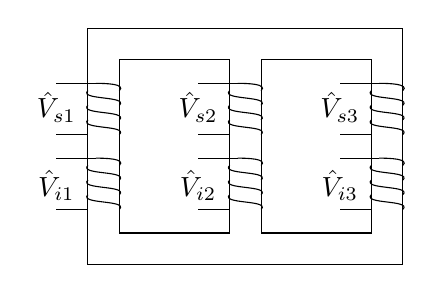
\begin{tikzpicture}
%grid
%\draw[gray,thick] (-1,-1) grid (5,3);
%\draw[gray,thin,xstep=0.1,ystep=0.1] (-1,-1) grid (5,3);
%transformer outer dimensions
\pgfmathsetmacro{\h}{3}
\pgfmathsetmacro{\w}{4}
\pgfmathsetmacro{\t}{0.4}
\pgfmathsetmacro{\g}{0.3}   %gap between coil and edge of window
\pgfmathsetmacro{\nL}{4}       %number of left hand turns
\pgfmathsetmacro{\nR}{3}      %number of right hand turns
%window size
\pgfmathsetmacro{\winH}{\h-2*\t}
\pgfmathsetmacro{\winW}{0.5*(\w-3*\t)}
%coil step
\pgfmathsetmacro{\stepHL}{0.5*(\h-2*\t-3*\g)/(\nL-0.5)}
\pgfmathsetmacro{\stepHR}{0.5*(\h-2*\t-3*\g)/(\nR-0.5)}

%transformer
\draw(0,0) rectangle (\w,\h);
\draw(\t,\t) rectangle ++(\winW,\winH);
\draw(2*\t+\winW,\t) rectangle ++(\winW,\winH);
%----------------------
%========================
%left leg TOP coil. top to bottom
\def\leftEdge{0};
\def\coilTop{\h-\t-\g};
%
\draw(\leftEdge+\t/4,\coilTop) to [out=0,in=45] (\leftEdge+\t,{\coilTop-\stepHL/2}); %top half section
%coil itself
\pgfmathsetmacro{\nLend}{\nL-2}
\foreach \y in { 0, ..., \nLend }{
\draw (\leftEdge,{\coilTop-\stepHL/2-\y*\stepHL}) to [out=-135,in=45] (\leftEdge+\t,{\coilTop-\stepHL/2-\y*\stepHL-\stepHL});
} 
%left hand terminals
\draw (\leftEdge+\t/4,\coilTop)--++(-1.25*\t,0) node(TA.A1){};
\draw (\leftEdge,\coilTop-\nL*\stepHL+0.5*\stepHL)--++(-1*\t,0)node(TA.A2){};
%--------------------
%left leg BOTTOM coil. top to bottom
\def\leftEdge{0};
\def\coilTop{\h-\t-2*\g-\nL*\stepHL+0.5*\stepHL};
%
\draw(\leftEdge+\t/4,\coilTop) to [out=0,in=45] (\leftEdge+\t,{\coilTop-\stepHL/2}); %top half section
%coil itself
\pgfmathsetmacro{\nLend}{\nL-2}
\foreach \y in { 0, ..., \nLend }{
\draw (\leftEdge,{\coilTop-\stepHL/2-\y*\stepHL}) to [out=-135,in=45] (\leftEdge+\t,{\coilTop-\stepHL/2-\y*\stepHL-\stepHL});
} 
%left hand terminals
\draw (\leftEdge+\t/4,\coilTop)--++(-1.25*\t,0) node(TA.B1){};
\draw (\leftEdge,\coilTop-\nL*\stepHL+0.5*\stepHL)--++(-1*\t,0)node(TA.B2){};
%==========================
%============================
%middle leg TOP coil. top to bottom
\def\leftEdge{\t+\winW};
\def\coilTop{\h-\t-\g};
%
\draw(\leftEdge+\t/4,\coilTop) to [out=0,in=45] (\leftEdge+\t,{\coilTop-\stepHL/2}); %top half section
%coil itself
\pgfmathsetmacro{\nLend}{\nL-2}
\foreach \y in { 0, ..., \nLend }{
\draw (\leftEdge,{\coilTop-\stepHL/2-\y*\stepHL}) to [out=-135,in=45] (\leftEdge+\t,{\coilTop-\stepHL/2-\y*\stepHL-\stepHL});
} 
%left hand terminals
\draw (\leftEdge+\t/4,\coilTop)--++(-1.25*\t,0) node(TB.A1){};
\draw (\leftEdge,\coilTop-\nL*\stepHL+0.5*\stepHL)--++(-1*\t,0)node(TB.A2){};
%--------------------
%middle  leg BOTTOM coil. top to bottom
\def\leftEdge{\t+\winW};
\def\coilTop{\h-\t-2*\g-\nL*\stepHL+0.5*\stepHL};
%
\draw(\leftEdge+\t/4,\coilTop) to [out=0,in=45] (\leftEdge+\t,{\coilTop-\stepHL/2}); %top half section
%coil itself
\pgfmathsetmacro{\nLend}{\nL-2}
\foreach \y in { 0, ..., \nLend }{
\draw (\leftEdge,{\coilTop-\stepHL/2-\y*\stepHL}) to [out=-135,in=45] (\leftEdge+\t,{\coilTop-\stepHL/2-\y*\stepHL-\stepHL});
} 
%left hand terminals
\draw (\leftEdge+\t/4,\coilTop)--++(-1.25*\t,0) node(TB.B1){};
\draw (\leftEdge,\coilTop-\nL*\stepHL+0.5*\stepHL)--++(-1*\t,0)node(TB.B2){};
%===========================
%============================
%right leg TOP coil. top to bottom
%========================
\def\leftEdge{\w-\t};
\def\coilTop{\h-\t-\g};
%
\draw(\leftEdge+\t/4,\coilTop) to [out=0,in=45] (\leftEdge+\t,{\coilTop-\stepHL/2}); %top half section
%coil itself
\pgfmathsetmacro{\nLend}{\nL-2}
\foreach \y in { 0, ..., \nLend }{
\draw (\leftEdge,{\coilTop-\stepHL/2-\y*\stepHL}) to [out=-135,in=45] (\leftEdge+\t,{\coilTop-\stepHL/2-\y*\stepHL-\stepHL});
} 
%left hand terminals
\draw (\leftEdge+\t/4,\coilTop)--++(-1.25*\t,0) node(TC.A1){};
\draw (\leftEdge,\coilTop-\nL*\stepHL+0.5*\stepHL)--++(-1*\t,0)node(TC.A2){};
%--------------------
%right leg BOTTOM coil. top to bottom
\def\leftEdge{\w-\t};
\def\coilTop{\h-\t-2*\g-\nL*\stepHL+0.5*\stepHL};
%
\draw(\leftEdge+\t/4,\coilTop) to [out=0,in=45] (\leftEdge+\t,{\coilTop-\stepHL/2}); %top half section
%coil itself
\pgfmathsetmacro{\nLend}{\nL-2}
\foreach \y in { 0, ..., \nLend }{
\draw (\leftEdge,{\coilTop-\stepHL/2-\y*\stepHL}) to [out=-135,in=45] (\leftEdge+\t,{\coilTop-\stepHL/2-\y*\stepHL-\stepHL});
} 
%left hand terminals
\draw (\leftEdge+\t/4,\coilTop)--++(-1.25*\t,0) node(TC.B1){};
\draw (\leftEdge,\coilTop-\nL*\stepHL+0.5*\stepHL)--++(-1*\t,0)node(TC.B2){};
%==========================
%===========================
%text
\draw (-0.4,1) node{$\hat{V}_{i1}$};
\draw (-0.4,2) node{$\hat{V}_{s1}$};
\draw (1.4,1) node{$\hat{V}_{i2}$};
\draw (1.4,2) node{$\hat{V}_{s2}$};
\draw (3.2,1) node{$\hat{V}_{i3}$};
\draw (3.2,2) node{$\hat{V}_{s3}$};
\end{tikzpicture}
\caption{ایک ہی قالب پر تین ٹرانسفارمر۔}
\label{شکل_ٹرانسفارمر_ایک_مرکز_تین-ٹرانسفارمر}
\end{figure}

شکل \حوالہ{شکل_ٹرانسفارمر_ستارہ_تکونی_جوڑ}-الف میں تین ٹرانسفارمر دکھائے گئے ہیں۔ان تین ٹرانسفارمر کے ابتدائی لچھے آپس میں دو طریقوں سے جوڑے جا سکتے ہیں۔ایک کو \اصطلاح{ستارہ نما} جوڑ\فرہنگ{ستارہ نما جوڑ}\فرہنگ{جوڑ!ستارہ نما}\حاشیہب{star connected}\فرہنگ{star connected} \عددیء{Y}  اور دوسرے کو \اصطلاح{تکونی} جوڑ\فرہنگ{تکونی جوڑ}\فرہنگ{جوڑ!تکونی}\حاشیہب{delta connected}\فرہنگ{delta connected}  \عددیء{\Delta}   کہتے ہیں۔اسی طرح ان تینوں ٹرانسفارمروں کے ثانوی  لچھے انہیں دو طریقوں سے جوڑے جا سکتے ہیں۔یوں انہیں جوڑنے کے چار ممکنہ طریقے ہیں یعنی
\begin{itemize}
\item
ستارہ:تکونی  \quad \عددیء{Y:\Delta}
\item
ستارہ:ستارہ \quad  \عددیء{Y:Y}
\item
تکونی:تکونی \quad  \عددیء{\Delta:\Delta}
\item
تکونی:ستارہ  \quad  \عددیء{\Delta:Y}
\end{itemize}

شکل \حوالہ{شکل_ٹرانسفارمر_ستارہ_تکونی_جوڑ}-الف میں ان تین ٹرانسفارمروں کے ابتدائی لچھوں کو ستارہ نما جوڑا گیا ہے جبکہ ان کی ثانوی لچھوں کو تکونی جوڑا گیا ہے۔شکل-ب میں تینوں ٹرانسفارمر کی ابتدائی لچھوں کو  ستارہ نما  دکھایا گیا ہے۔اسی طرح ثانوی لچھوں کو تکونی  دکھایا گیا ہے۔انہی شکلوں کی وجہ سے ان کو ستارہ نما جوڑ اور تکونی جوڑ کہتے ہیں۔

ایسی شکل بناتے وقت تینوں ٹرانسفارمروں کے ابتدائی لچھے کو جس زاویہ پر بنایا جاتا ہے اس کے ثانوی لچھے کو بھی اُسی زاویہ پر بنایا جاتا ہے۔یوں شکل کے حصہ الف میں سب سے اوپر ٹرانسفارمر جس کے ابتدائی جانب کے  سرے \عددیء{an} اور ثانوی جانب  کے سرے \عددیء{a'n'} ہیں کو حصہ با میں صفر زاویہ پر بنایا گیا ہے۔تین  مرحلہ ٹرانسفارمروں کو اس طرح کی علامتوں سے ظاہر کیا جاتا ہے اور ان میں قالب نہیں دکھایا جاتا۔

ٹرانسفارمر کے جوڑ بیان کرتے وقت بائیں جانب کے جوڑ کو پہلے اور دائیں جانب کی جوڑ کو بعد میں پکارتے ہیں۔یوں شکل میں ٹرانسفارمر کو ستارہ-تکونی جُڑا ٹرانسفارمر کہیں گے۔اسی طرح ابتدائی جانب کو بائیں اور ثانوی جانب کو دائیں ہاتھ بنایا جاتا ہے۔یوں اس شکل میں ابتدائی جانب ستارہ نما ہے جبکہ ثانوی جانب تکونی ہے۔
\begin{figure}
\centering
%\includegraphics[width=\linewidth]{figTransformersStarDeltaConnections}
\begin{tikzpicture}[scale=0.75]
%grid
%\draw[gray,thick] (-3,-3) grid (12,5);
%\draw[gray,thin,xstep=0.1,ystep=0.1] (-3,-3) grid (12,5);
%transformer outer dimensions
\pgfmathsetmacro{\l}{1.5}
\pgfmathsetmacro{\s}{0.5}
\pgfmathsetmacro{\arm}{2}
\pgfmathsetmacro{\shiftX}{9cm}
\pgfmathsetmacro{\shiftY}{1.25 cm}
\pgfmathsetmacro{\gap}{3.5 cm}
\pgfmathsetmacro{\startDelX}{-\arm/2}
\pgfmathsetmacro{\startDelY}{-\arm/3}
\draw node at (11.5,-2) {الف};
\draw node at (0,-2) {ب};
%
\begin{scope}[xshift=\shiftX]
\draw (0,0) node  [transformer core](T1){}; 
\draw (0,2.5) node  [transformer core](T2){}; 
\draw (0,5) node  [transformer core](T3){}; 
\draw(T1.base) node {$\bullet \hspace{2mm} \bullet$};
\draw(T2.base) node {$\bullet \hspace{2mm} \bullet$};
\draw(T3.base) node {$\bullet \hspace{2mm} \bullet$};
%
\draw(T1.A1) to [short,-o] ++(-\l,0) node[left](c) {$c$};
\draw(T2.A1) to [short,-o] ++(-\l,0) node[left](b) {$b$};
\draw(T3.A1) to [short,-o] ++(-\l,0) node[left] (a){$a$};
%
\draw(T1.A2) to [short,-*] ++(-\s,0) coordinate (k1){};
\draw(T2.A2) to [short,-*] ++(-\s,0)coordinate (k2){};
\draw(T3.A2) to [short] ++(-\s,0)coordinate (k3){};
%
\draw(k3) to [short] (k2) to [short] (k1) to [short,-o] ++(-\l+\s,0)node[left](n){$n$};
%text
\node[right] at ($(a) ! 0.5 ! (b)$) {$
\begin{aligned}
&+\\
&v_{ab}\\
&-
\end{aligned}
$};
%
\node[right] at ($(b) ! 0.5 ! (c)$) {$
\begin{aligned}
&+\\
&v_{bc}\\
&-
\end{aligned}
$};
%
\node at ($(T1.A1) ! 0.5 ! (T1.A2)$){$
\begin{aligned}
&+\\
&v_{cn}\\
&-
\end{aligned}
$};
%
\node at ($(T2.A1) ! 0.5 ! (T2.A2)$){$
\begin{aligned}
&+\\
&v_{bn}\\
&-
\end{aligned}
$};
%
\node at ($(T3.A1) ! 0.5 ! (T3.A2)$){$
\begin{aligned}
&+\\
&v_{an}\\
&-
\end{aligned}
$};
%right hand side
\draw(T1.B1) to [short,-o] ++(\l,0)  node[right](c'){$c'$};
\draw(T2.B1) to [short,-o] ++(\l,0)node[right](b'){$b'$};
\draw(T3.B1) to [short,-o] ++(\l,0) node [right](a'){$a'$};
%;
\draw(T1.B2) to [short] ++(\s,0) to [short,-*] ++(0,7.1);
\draw(T2.B2) to [short,-*] (T1.B1);
\draw(T3.B2) to [short,-*] (T2.B1);
%text
\draw node at ($(a') ! 0.5 ! (b')$){$
\begin{aligned}
&+\\
&v_{ab}'\\
&-
\end{aligned}
$};
%
\draw node at ($(b') ! 0.5 ! (c')$){$
\begin{aligned}
&+\\
&v_{bc}'\\
&-
\end{aligned}
$};
\end{scope}
%=====================
\begin{scope}[yshift=\shiftY]
%star
\draw (0,0) to [inductor,l={$- v_{an} +$}] ++(0:\arm)node [below left] {$\bullet$} to [short] ++(0,-2.2) to [short,-o]++(-4,0) node[left] {$a$};
\draw (0,0) to [inductor,l={$+ v_{cn} -$}] ++(120:\arm) node [right]{$\bullet$} to [short,-o] ++(-1,0) node [left] {$c$};
\draw (0,0) to [inductor,l={$+ v_{bn} -$}] ++(-120:\arm) node [above left] {$\bullet$} to [short,-o] ++(-1,0)node [left]{$b$};
\draw (0,0) to [short,*-o] ++(-0.5,0) node [left]{$n$};
\draw(2,2) node {$Y:\Delta$};
%delta
\begin{scope}[xshift=\gap]
\draw (\startDelX,\startDelY) to [inductor,l_={$- v_{ab}'+$}] ++(0:\arm)coordinate(delA){} to [inductor] ++(120:\arm)coordinate(delB){}  to [inductor] ++(-120:\arm);
\path  (30:0.6*\arm)  node[rotate=-60] {$+ v_{ca}' -$}; 
\path  (150:0.6*\arm)  node[rotate=60] {$+ v_{bc}' -$}; 
\draw (delA) to [short,-o] ++(\s,0) node[right]{$a'$};
\draw (delB) to [short] ++(0,0.5) to [short,-o] ++(1.5,0) node[right]{$c'$};
\draw (\startDelX,\startDelY) to [short] ++(0,-0.75) to [short,-o] ++(\l+1,0)node[right]{$b'$};
\draw[below left]  node at (delA){$\bullet$};
\draw[right]  node at (delB){$\bullet$};
\draw[above]  node at (\startDelX,\startDelY){$\bullet$};
\end{scope}
\end{scope}
\end{tikzpicture}
\caption{تین مرحلہ ستارہ-تکونی ٹرانسفارمر}
\label{شکل_ٹرانسفارمر_ستارہ_تکونی_جوڑ}
\end{figure}


	ستارہ نما جڑی جانب سے چار برقی تاریں نکلتی ہیں۔اس جانب لچھوں کے مشترکہ سرا \عددیء{n} کو عموماً ٹرانسفارمر کے نزدیک زمین میں گہرائی تک دھنسا دیا جاتا ہے۔اس تار کو \اصطلاح{زمینی تار}\فرہنگ{زمینی تار}\حاشیہب{ground}\فرہنگ{ground wire}  یا صرف \اصطلاح{زمین}\فرہنگ{زمین}\حاشیہب{ground, earth,neutral}\فرہنگ{earth}  کہتے ہیں۔عام فہم میں اسے \اصطلاح{ٹھنڈی تار}\فرہنگ{ٹھنڈی تار}\حاشیہب{neutral} کہتے ہیں۔باقی تین یعنی \عددیء{a,b,c}  \اصطلاح{گرم تار}\فرہنگ{گرم تار}\حاشیہب{live wires} کہلاتے ہیں۔

ٹرانسفارمر کی لچھے پر برقی دباو کو \اصطلاح{یک مرحلہ برقی دباو}\فرہنگ{یک مرحلہ برقی دباو} \عددیء{\hat{V}_{\textup{یکمرحلہ}}}\حاشیہب{phase voltage}\فرہنگ{phase voltage} کہتے ہیں اور لچھے میں برقی رو کو \اصطلاح{یک مرحلہ برقی رو}\فرہنگ{یک مرحلہ برقی رو} \عددیء{\hat{I}_{\textup{یکمرحلہ}}}\حاشیہب{phase current}\فرہنگ{phase current}  کہتے ہیں۔ جبکہ ٹرانسفارمر سے باہر نکلتی کسی دو گرم تاروں کے مابین برقی دباو کو \اصطلاح{تار کی برقی دباو}\فرہنگ{تار کی برقی دباو} \عددیء{\hat{V}_{\textup{تار}}}\حاشیہب{line to line voltage}\فرہنگ{line voltage} کہتے ہیں اور کسی بھی گرم تار میں برقی رو کو \اصطلاح{تار کی برقی رو}\فرہنگ{تار کی برقی رو} \عددیء{\hat{I}_{\textup{تار}}}\حاشیہب{line current}\فرہنگ{line current}  کہتے ہیں۔ زمینی تار میں برقی رو کو \اصطلاح{زمینی برقی رو}\فرہنگ{زمینی برقی رو}  \عددیء{\hat{I}_{\textup{زمینی}}}\حاشیہب{ground current}\فرہنگ{ground current} کہتے ہیں۔

ستارہ نما \عددیء{Y} جانب \اصطلاح{یک مرحلہ} مقداروں اور \اصطلاح{تار} کی مقداروں  کا آپس میں یوں رشتہ ہے
\begin{gather}
\begin{aligned}\label{مساوات_ستارہ_ٹرانسفارمر_تار_اور_دور_رشتے}
V_{\textup{تار}}&=\sqrt{3} V_{\textup{یکمرحلہ}}\\
I_{\textup{تار}}&=I_{\textup{یکمرحلہ}}
\end{aligned}
\end{gather}
جبکہ تکونی \عددیء{\Delta} جانب یک مرحلہ اور تار کی مقداروں کا آپس میں یوں رشتہ ہے
\begin{gather}
\begin{aligned}\label{مساوات_تکونی_ٹرانسفارمر_تار_اور_دور_رشتے}
V_{\textup{تار}}&= V_{\textup{یکمرحلہ}}\\
I_{\textup{تار}}&=\sqrt{3} I_{\textup{یکمرحلہ}}
\end{aligned}
\end{gather}
یہ مرحلی سمتیہ کے رشتے نہیں بلکہ ان کی غیر سمتی قیمتوں کے رشتے ہیں۔ان دو مساواتوں سے حاصل ہوتا ہے
\begin{align}
V_{\textup{تار}} I_{\textup{تار}}=\sqrt{3} V_{\textup{یکمرحلہ}} I_{\textup{یکمرحلہ}}
\end{align}
چونکہ ایک مرحلہ ٹرانسفارمر کی وولٹ-ایمپیئر \عددیء{V_{\textup{یکمرحلہ}} I_{\textup{یکمرحلہ}}} ہیں اور ایسے تین ٹرانسفارمر مل کر ایک تین مرحلہ ٹرانسفارمر بناتے ہیں لہٰذا تین  مرحلہ ٹرانسفارمر کی وولٹ-ایمپیئر اس کے تین گنا ہوں گے یعنی
\begin{align}
\textup{وولٹ-ایمپیئر}= 
3 V_{\textup{یکمرحلہ}} I_{\textup{یکمرحلہ}}= 
3 \times \frac{V_{\textup{تار}} I_{\textup{تار}}}{\sqrt{3}}=
\sqrt{3} V_{\textup{تار}} I_{\textup{تار}}
\end{align}
یہ مساوات \اصطلاح{تین مرحلہ} ادوار  میں عام استعمال ہوتی ہے۔

	ٹرانسفارمر کسی طرح بھی جوڑے جائیں وہ اپنی بنیادی کارکردگی تبدیل نہیں کرتے لہٰذا انہیں ستارہ نما یا تکونی جوڑنے کے بعد بھی ان میں ہر ایک ٹرانسفارمر انفرادی طور پر صفحہ \حوالہصفحہ{مساوات_ٹرانسفارمر_تبادلہ_دباو_رو} پر دئے مساوات \حوالہ{مساوات_ٹرانسفارمر_تبادلہ_دباو_رو}  اور صفحہ \حوالہصفحہ{مساوات_ٹرانسفارمر_متبادل_رکاوٹ_تعریف} پر دئے مساوات \حوالہ{مساوات_ٹرانسفارمر_متبادل_رکاوٹ_تعریف}  پر پورے اترے گا۔انہیں استعمال کر کے شکل \حوالہ{شکل_ٹرانسفارمر_تین_دور_ٹرانسفارمر_کے_مختلف_جوڑ}  میں دیئے گئے ٹرانسفارمروں کے ابتدائی اور ثانوی جانب کی یک مرحلہ اور تار کی مقداروں کے رشتے حاصل کئے جا سکتے ہیں۔اس شکل میں \عددیء{a=N_1/N_2} ہے جہاں  \عددیء{N_1:N_2} ان میں ایک مرحلہ ٹرانسفارمر کے چکر کی نسبت ہے۔تین مرحلہ ٹرانسفارمر پر لگی تختی پر دونوں جانب تار کی برقی دباو کی نسبت لکھی جاتی ہے۔
\begin{figure}
\centering
%\includegraphics[width=\linewidth]{figTransformersAllPossibleConnections}
\begin{tikzpicture}[scale=0.6]
%grid
%\draw[gray,thick] (-3,-3) grid (18,5);
%\draw[gray,thin,xstep=0.1,ystep=0.1] (-3,-3) grid (18,5);
%transformer outer dimensions
\pgfmathsetmacro{\shiftX}{12 cm}
\pgfmathsetmacro{\shiftY}{5 cm}

\pgfmathsetmacro{\arm}{2}
\pgfmathsetmacro{\con}{2.5}
\pgfmathsetmacro{\conStarS}{\con-\arm*cos(30)}                  %one arm of star is at ninty degree
\pgfmathsetmacro{\conStarL}{\con+\arm*cos(30)}
\pgfmathsetmacro{\h}{sqrt(3)/2*\arm}
\pgfmathsetmacro{\conDeltaS}{\con-\arm/sqrt(3)}                      %one arm of delta is at 90 degree as h=sqrt{3}/2*\arm
\pgfmathsetmacro{\conDeltaL}{\con+\arm/sqrt(12)}
\pgfmathsetmacro{\conDeltaZeroS}{\con-\arm*cos(60)}    %one arm of delta is at 0 degree as h=sqrt{3}/2*\arm
\pgfmathsetmacro{\conDeltaZeroM}{\con}
\pgfmathsetmacro{\conDeltaZeroL}{\con+\arm*cos(60)}


\pgfmathsetmacro{\gap}{4 cm}        %gap between star and delta centres
\pgfmathsetmacro{\startNintyX}{-\h/3}    %start of delta if one arm is at 90 degrees
\pgfmathsetmacro{\startNintyY}{-\arm/2}
\pgfmathsetmacro{\startZeroX}{-\arm/2}   %start of delta if one arm is at 0 degrees
\pgfmathsetmacro{\startZeroY}{-\h/3} 

%===================
%STAR-DELTA
\begin{scope}[yshift=\shiftY]
%star at 90 degrees
\draw (0,0) to [short] ++(-90:\arm)coordinate (starA){} to [short,-o,i<={$I$}] ++(180:\con)coordinate (starAend){};
\draw (0,0) to [short] ++(30:\arm)coordinate (starB){} to [short] ++(0,0.5) to [short,-o]++(180:\conStarL)coordinate (starBend){};
\draw (0,0) to [short] ++(150:\arm)coordinate (starC){} to  [short,-o]++(180:\conStarS)coordinate (starCend){};
%text
\draw[<->](-2,1)--(-2,-2) node[fill=white,pos=0.5]{$V$};
\draw[gray] (-0.1,0)--(-1,0);
\draw[<->](-0.6,0)--(-0.6,-2) node[fill=white,pos=0.5]{$\frac{V}{\sqrt{3}}$};
%=================
%delta at 90 degrees
\begin{scope}[xshift=\gap]
\draw (\startNintyX,\startNintyY)coordinate (deltaNintyA){} to [short] ++(30:\arm)coordinate (deltaNintyB){} to [short] ++(150:\arm)coordinate (deltaNintyC){} to [short,i={$aI$}]++(-90:\arm);
\draw (deltaNintyA) to [short]++(0,-0.5) to [short,-o,i={$\sqrt{3} a I$}] ++(\conDeltaL,0);
\draw (deltaNintyB) to [short,-o] ++(\conDeltaS,0);
\draw (deltaNintyC) to [short]++(0,0.5) to [short,-o] ++(\conDeltaL,0);
\draw[<->](1.6,0)--(1.6,1.5) node [fill=white,pos=0.5]{$\frac{V}{\sqrt{3} a}$};
\end{scope}
%=================================
%=================================
%DELTA-STAR
\begin{scope}[xshift=\shiftX+\gap, xscale=-1, yscale=1]
%star at 90 degrees
\draw (0,0) to [short] ++(-90:\arm)coordinate (starA){} to [short,-o,i<={$\frac{aI}{\sqrt{3}}$}] ++(180:\con)coordinate (starAend){};
\draw (0,0) to [short] ++(30:\arm)coordinate (starB){} to [short] ++(0,0.5) to [short,-o]++(180:\conStarL)coordinate (starBend){};
\draw (0,0) to [short] ++(150:\arm)coordinate (starC){} to  [short,-o]++(180:\conStarS)coordinate (starCend){};
%text
\draw[<->](-2,1)--(-2,-2) node[fill=white,pos=0.5]{$\frac{\sqrt{3}V}{a}$};
\draw[gray] (-0.1,0)--(-1,0);
\draw[<->](-0.5,0)--(-0.5,-2) node[fill=white,pos=0.5]{$\frac{V}{a}$};
%=================
%delta at 90 degrees
\begin{scope}[xshift=\gap]
\draw (\startNintyX,\startNintyY)coordinate (deltaNintyA){} to [short] ++(30:\arm)coordinate (deltaNintyB){} to [short] ++(150:\arm)coordinate (deltaNintyC){} to [short,i<={$\frac{I}{\sqrt{3}}$}]++(-90:\arm);
\draw (deltaNintyA) to [short]++(0,-0.5) to [short,-o,i={$I$}] ++(\conDeltaL,0);
\draw (deltaNintyB) to [short,-o] ++(\conDeltaS,0);
\draw (deltaNintyC) to [short]++(0,0.5) to [short,-o] ++(\conDeltaL,0);
\draw[<->](1.5,0)--(1.5,1.5) node [fill=white,pos=0.5]{$V$};
\end{scope}
\end{scope}
%----======----
\end{scope}
%====================
%===================
%===================
%LOWER TWO FIGURES
%STAR-STAR
%star at 90 degrees
\draw (0,0) to [short] ++(-90:\arm)coordinate (starA){} to [short,-o,i<={$I$}] ++(180:\con)coordinate (starAend){};
\draw (0,0) to [short] ++(30:\arm)coordinate (starB){} to [short] ++(0,0.5) to [short,-o]++(180:\conStarL)coordinate (starBend){};
\draw (0,0) to [short] ++(150:\arm)coordinate (starC){} to  [short,-o]++(180:\conStarS)coordinate (starCend){};
%text
\draw[<->](-2,1)--(-2,-2) node[fill=white,pos=0.5]{$V$};
\draw[gray] (-0.1,0)--(-1,0);
\draw[<->](-0.6,0)--(-0.6,-2) node[fill=white,pos=0.5]{$\frac{V}{\sqrt{3}}$};
%=================
\begin{scope}[xshift=\gap,xscale=-1,yscale=1]
%star at 90 degrees
\draw (0,0) to [short] ++(-90:\arm)coordinate (starA){} to [short,-o,i<={$a I$}] ++(180:\con)coordinate (starAend){};
\draw (0,0) to [short] ++(30:\arm)coordinate (starB){} to [short] ++(0,0.5) to [short,-o]++(180:\conStarL)coordinate (starBend){};
\draw (0,0) to [short] ++(150:\arm)coordinate (starC){} to  [short,-o]++(180:\conStarS)coordinate (starCend){};
%text
\draw[<->](-2,1)--(-2,-2) node[fill=white,pos=0.5]{$\frac{V}{a}$};
\draw[gray] (-0.1,0)--(-1,0);
\draw[<->](-0.8,0)--(-0.8,-2) node[fill=white,pos=0.5]{$\frac{V}{a\sqrt{3}}$};
\end{scope}
%
 % DELTA-DELTA
%delta
\begin{scope}[xshift=\shiftX]
\draw(\startZeroX,\startZeroY)coordinate(deltA){} to [short,i={$\frac{I}{\sqrt{3}} $}] ++(0:\arm)coordinate(deltB){} to [short]++(120:\arm)coordinate(deltC){} to [short] ++(-120:\arm);
\draw[short] (deltA) to [short,-o]++(180:\conDeltaZeroS);
\draw[short] (deltB) to [short] ++(0,-0.5) to [short,-o]++(180:\conDeltaZeroL);
\draw[short] (deltC) to [short] ++(0,0.5) to [short,-o,i<={$I$}]++(180:\conDeltaZeroM);
\draw[<->] (-2,-0.65) --++(0,2.2)node[fill=white,pos=0.5]{$V$};
%delta
\begin{scope}[xshift=\gap,xscale=-1,yscale=1]
\draw(\startZeroX,\startZeroY)coordinate(deltA){} to [short,i={$\frac{a I}{\sqrt{3}} $}] ++(0:\arm)coordinate(deltB){} to [short]++(120:\arm)coordinate(deltC){} to [short] ++(-120:\arm);
\draw[short] (deltA) to [short,-o]++(180:\conDeltaZeroS);
\draw[short] (deltB) to [short] ++(0,-0.5) to [short,-o]++(180:\conDeltaZeroL);
\draw[short] (deltC) to [short] ++(0,0.5) to [short,-o,i<={$a I$}]++(180:\conDeltaZeroM);
\draw[<->] (-2,-0.65) --++(0,2.2)node[fill=white,pos=0.5]{$\tfrac{V}{a}$};
\end{scope}
\end{scope}
\end{tikzpicture}
\caption{ابتدائی اور ثانوی جانب تار اور یک مرحلہ مقداروں کے رشتے۔}
\label{شکل_ٹرانسفارمر_تین_دور_ٹرانسفارمر_کے_مختلف_جوڑ}
\end{figure}


جیسے شکل \حوالہ{شکل_ٹرانسفارمر_تین_دور_ٹرانسفارمر_کے_مختلف_جوڑ} میں دکھایا گیا ہے ستارہ-تکونی ٹرانسفارمر کی تار پر برقی دباو کی نسبت
\begin{align}
\frac{V_\textup{{ابتدائی}}}{V_\textup{{ثانوی}}}=\sqrt{3} a =\sqrt{3} \left(\frac{N_1}{N_2} \right)
\end{align}
جبکہ ستارہ-ستارہ کا
\begin{align}
\frac{V_\textup{{ابتدائی}}}{V_\textup{{ثانوی}}}=a =\left(\frac{N_1}{N_2} \right)
\end{align}
تکونی-ستارہ کا
\begin{align}
\frac{V_\textup{{ابتدائی}}}{V_\textup{{ثانوی}}}=\frac{a}{\sqrt{3}}=\frac{1}{\sqrt{3}} \left(\frac{N_1}{N_2} \right)
\end{align}
اور تکونی-تکونی کا
\begin{align}
\frac{V_\textup{{ابتدائی}}}{V_\textup{{ثانوی}}}=a =\left(\frac{N_1}{N_2} \right)
\end{align}
ہے۔
%
\ابتدا{مثال}
یک مرحلہ  تین یکساں ٹرانسفارمروں کو ستارہ-تکونی \عددیء{Y:\Delta}  جوڑ کر تین مرحلہ ٹرانسفارمر بنایا گیا ہے۔ایک مرحلہ ٹرانسفارمر کی برقی \اصطلاح{سکت}\فرہنگ{سکت}\حاشیہب{rating}\فرہنگ{rating} درج ذیل ہے:
\begin{align*}
\SI{50}{\kilo \volt \ampere} , \quad 6350:440\,\textup{V}, \quad \SI{50}{\hertz}
\end{align*}
ستارہ-تکونی ٹرانسفارمر کی ابتدائی جانب \عددیء{11000}  وولٹ کی تین مرحلہ تار کی برقی دباو لاگو کیا گیا۔اس تین مرحلہ ٹرانسفارمر کی ثانوی جانب تار کا برقی دباو معلوم کریں۔

حل: حل کرتے وقت ہم ایک  عدد  یک مرحلہ ٹرانسفارمر پر نظر رکھیں گے۔ ابتدائی جانب اگر یک مرحلہ ٹرانسفارمر پر غور کیا جائے تو
\begin{align*}
\frac{N_1}{N_2}=\frac{V_1}{V_2}=\frac{6350}{440}
\end{align*}
اور اس پر لاگو برقی دباو مساوات \حوالہ{مساوات_ستارہ_ٹرانسفارمر_تار_اور_دور_رشتے}  کی مدد سے
\begin{align*}
V_{\textup{\RL{ابتدائی، یکمرحلہ}}}=\frac{V_{\textup{تار}}}{\sqrt{3}}=\frac{11000}{\sqrt{3}}=\SI{6350.85}{\volt}
\end{align*}
ہے لہٰذا اس یک مرحلہ ٹرانسفارمر کی ثانوی جانب مساوات \حوالہ{مساوات_ٹرانسفارمر_تبادلہ_دباو_رو} کی مدد سے
\begin{align*}
V_{\textup{ثانوی}}=\frac{N_2}{N_1} V_{\textup{ابتدائی}}=\frac{440}{6350} \times 6350.85 \approx \SI{440}{\volt}
\end{align*}
ہیں۔چونکہ ثانوی جانب ان تین یک مرحلہ ٹرانسفارمروں کو تکونی جوڑا گیا ہے لہٰذا مساوات \حوالہ{مساوات_تکونی_ٹرانسفارمر_تار_اور_دور_رشتے}  کی مدد سے اس جانب تار کی برقی دباو یہی ہو گی۔اس تین مرحلہ ٹرانسفارمر کی تار پر برقی دباو کی نسبت
\begin{align*}
\frac{V_{\text{\RL{ابتدائی، تار}}}}{V_{\textup{ثانوی، تار}}}=\frac{11000}{440}
\end{align*}
ہے۔چونکہ یک مرحلہ ٹرانسفارمر \عددیء{50}  کلو وولٹ-ایمپیئر کا ہے لہٰذا یہ تین مرحلہ ٹرانسفارمر  \عددیء{150} کلو وولٹ-ایمپیئر کا ہو گا۔یوں اس تین مرحلہ ٹرانسفارمر کی سکت\فرہنگ{سکت}\حاشیہب{rating}\فرہنگ{rating}
\begin{align*}
\SI{150}{\kilo \volt \ampere}, \quad 11000:440\,\textup{V},\quad \SI{50}{\hertz}
\end{align*}
ہو گی۔

	ٹرانسفارمر پر لگی تختی\فرہنگ{تختی}\حاشیہب{name plate}\فرہنگ{name plate} پر اس کی سکت بیان ہوتی ہے جس میں ٹرانسفارمر کے دونوں جانب تار کے برقی دباو لکھے جاتے ہیں نہ کہ لچھوں کے چکر۔
\انتہا{مثال}
%
ستارہ-ستارہ جڑے ٹرانسفارمر عام طور استعمال نہیں ہوتے۔اس کی وجہ یہ ہے کہ اگرچہ ان کی تین مرحلہ برقی دباو  کے بنیادی جزو آپس میں \عددیء{120\degree}  زاویائی فاصلے پر ہوتے ہیں لیکن ان کی تیسری موسیقائی جزو آپس میں ہم قدم ہوتی ہیں۔قالب کی غیر بتدریج خصوصیات کی وجہ سے ٹرانسفارمر میں ہر صورت تیسری موسیقائی جزو پائے جاتے ہیں۔تیسری موسیقائی جزو ہم قدم ہونے کی وجہ سے جمع ہو کر ایک نہایت بڑی برقی دباو کی موج پیدا کرتے ہیں جو کبھی کبھی برقی دباو کی بنیادی جزو سے بھی زیادہ بڑھ جاتی ہے۔

بقایا تین قسم کے جڑے ٹرانسفارمروں میں برقی دباو کی تیسری موسیقائی جزو مسئلہ نہیں کرتیں چونکہ ان میں تکونی جُڑے لچھوں میں برقی رو گھومنے شروع ہو جاتی ہے جو ان کے اثر کو ختم کر دیتی ہے۔

تین مرحلہ ٹرانسفارمر کے متوازن دور حل کرتے وقت ہم تصور کرتے ہیں کہ ٹرانسفارمر ستارہ نما جڑا  ہے۔یوں اس کے ایک مرحلے میں برقی رو، تار  کی برقی رو ہی ہو گی اور اس کے ایک مرحلے پر لاگو برقی دباو، یک مرحلہ برقی دباو  ہو گا۔اسی طرح ہم تصور کرتے ہیں کہ اس پر لدا برقی بوجھ بھی ستارہ نما جُڑا ہے۔یوں تین مرحلہ کی جگہ ہم یک مرحلہ دور کا نسبتاً آسان مسئلہ حل کرتے ہیں۔ ایسا کرنے سے مسئلہ پر غور کرنا آسان ہو جاتا ہے۔یہ ایک مثال سے زیادہ بہتر سمجھ آئے گا۔
%
\ابتدا{مثال}
ایک تین مرحلہ \عددیء{\Delta :Y}   \عددیء{2000} کلو وولٹ-ایمپیئر،  \عددیء{11000:600 }  وولٹ اور \عددیء{50} ہرٹز پر چلنے والا کامل ٹرانسفارمر تین مرحلہ کے متوازن برقی بوجھ کو طاقت مہیا کر رہا ہے۔یہ بوجھ تکونی جڑا ہے جہاں بوجھ کا ہر حصہ \عددیء{(0.504+j0.1917)} کے برابر ہے۔شکل \حوالہ{شکل_ٹرانسفارمر_تکونی_بار_کی_مثال}  میں یہ دکھایا گیا ہے۔
\begin{itemize}
\item
اس شکل میں ہر جگہ برقی رو معلوم کریں۔
\item
برقی بوجھ\فرہنگ{بوجھ}\حاشیہب{electrical load}\فرہنگ{load} کو درکار طاقت معلوم کریں
\end{itemize}

\begin{figure}
\centering
%\includegraphics[width=\linewidth]{figTransformersDeltaLoadedExample}
\begin{tikzpicture}[scale=0.75]
%grid
%\draw[gray,thick] (-3,-3) grid (18,5);
%\draw[gray,thin,xstep=0.1,ystep=0.1] (-3,-3) grid (18,5);
%transformer outer dimensions
\pgfmathsetmacro{\shiftX}{9 cm}
\pgfmathsetmacro{\shiftY}{6.5 cm}

\pgfmathsetmacro{\arm}{2}
\pgfmathsetmacro{\con}{2.5}
\pgfmathsetmacro{\conStarS}{\con-\arm*cos(30)}                  %one arm of star is at ninty degree
\pgfmathsetmacro{\conStarL}{\con+\arm*cos(30)}
\pgfmathsetmacro{\h}{sqrt(3)/2*\arm}
\pgfmathsetmacro{\conDeltaS}{\con-\arm/sqrt(3)}                      %one arm of delta is at 90 degree as h=sqrt{3}/2*\arm
\pgfmathsetmacro{\conDeltaL}{\con+\arm/sqrt(12)}
\pgfmathsetmacro{\conDeltaZeroS}{\con-\arm*cos(60)}    %one arm of delta is at 0 degree as h=sqrt{3}/2*\arm
\pgfmathsetmacro{\conDeltaZeroM}{\con}
\pgfmathsetmacro{\conDeltaZeroL}{\con+\arm*cos(60)}


\pgfmathsetmacro{\gap}{3 cm}        %gap between star and delta centres
\pgfmathsetmacro{\startNintyX}{-\h/3}    %start of delta if one arm is at 90 degrees
\pgfmathsetmacro{\startNintyY}{-\arm/2}
\pgfmathsetmacro{\startZeroX}{-\arm/2}   %start of delta if one arm is at 0 degrees
\pgfmathsetmacro{\startZeroY}{-\h/3} 


\node at (0.6,2){$11000:600V$}; 
%DELTA TRANSFORMER
\draw (\startZeroX,\startZeroY)coordinate(delA){} to [inductor] ++(0:\arm)coordinate(delB){} to [inductor] ++(120:\arm)coordinate(delC){} to [inductor] ++(-120:\arm);
\draw (delA) to [short,-o]++(180:\conDeltaZeroS);
\draw (delB) to [short] ++(0,-0.5) to [short,-o]++(180:\conDeltaZeroL);
\draw (delC) to [short,-o]++(180:\conDeltaZeroM);
%STAR TRANSFORMER
\begin{scope}[xshift=\gap]
\draw (0,0)node[below right]{$n$} to [inductor] ++(0:\arm) coordinate(starA){};
\draw (0,0) to [inductor] ++(120:\arm)  to [short] ++(0,0.5) coordinate(starB){};
\draw (0,0) to [inductor] ++(-120:\arm) to [short] ++(0,-0.5)coordinate(starC){};
\end{scope}
%DELTA LOAD
\begin{scope}[xshift=\shiftX]
\draw(2*\startZeroX,2*\startZeroY) coordinate(loadAa){} to [resistor,l_={$0.504$}] ++(0:\arm) to [inductor,l_={$j 0.1917$}] ++(0:\arm)coordinate(loadBb){} to [resistor] ++(120:\arm) to [inductor] ++(120:\arm)coordinate(loadCc){} to [resistor] ++(-120:\arm) to [inductor] ++(-120:\arm);
\end{scope}
\draw (starA) -| (loadAa);
\draw (starB) |- (loadCc);
\draw (starC) -| (loadBb);
\end{tikzpicture}
\caption{ٹرانسفارمر تکونی متوازن بوجھ کو طاقت فراہم کر رہا ہے۔}
\label{شکل_ٹرانسفارمر_تکونی_بار_کی_مثال}
\end{figure}
حل:

پہلے تکونی بوجھ کو ستارہ نما بوجھ میں تبدیل کرتے ہیں
\begin{align*}
Z_Y= \frac{Z_\Delta}{3}=\frac{0.504+j0.1917}{3}=0.168+j0.0639
\end{align*}
اس بوجھ کو ستارہ نما جڑا شکل \حوالہ{شکل_ٹرانسفارمر_تکونی_بار_کو_ستارہ_تبادلہ} میں دکھایا گیا ہے۔اس شکل میں ایک برقی تار جسے نقطہ دار لکیر سے ظاہر کیا گیا ہے کو ٹرانسفارمر کی زمینی نقطہ سے بوجھ کے مشترکہ سرے کے درمیان جڑا دکھایا گیا ہے۔متوازن دور میں اس تار میں برقی رو صفر ہو گی۔حل کرنے کی نیت سے ہم اس متوازن دور سے ایک مرحلہ لے کر حل کرتے ہیں۔
\begin{figure}
\centering
%\includegraphics[width=\linewidth]{figTransformersDeltaLoadedExampleTurnedStar}
\begin{tikzpicture}[scale=0.75]
%grid
%\draw[gray,thick] (-3,-3) grid (18,5);
%\draw[gray,thin,xstep=0.1,ystep=0.1] (-3,-3) grid (18,5);
%transformer outer dimensions
\pgfmathsetmacro{\shiftX}{9 cm}
\pgfmathsetmacro{\shiftY}{6.5 cm}

\pgfmathsetmacro{\arm}{2}
\pgfmathsetmacro{\con}{2.5}
\pgfmathsetmacro{\conStarS}{\con-\arm*cos(30)}                  %one arm of star is at ninty degree
\pgfmathsetmacro{\conStarL}{\con+\arm*cos(30)}
\pgfmathsetmacro{\h}{sqrt(3)/2*\arm}
\pgfmathsetmacro{\conDeltaS}{\con-\arm/sqrt(3)}                      %one arm of delta is at 90 degree as h=sqrt{3}/2*\arm
\pgfmathsetmacro{\conDeltaL}{\con+\arm/sqrt(12)}
\pgfmathsetmacro{\conDeltaZeroS}{\con-\arm*cos(60)}    %one arm of delta is at 0 degree as h=sqrt{3}/2*\arm
\pgfmathsetmacro{\conDeltaZeroM}{\con}
\pgfmathsetmacro{\conDeltaZeroL}{\con+\arm*cos(60)}


\pgfmathsetmacro{\gap}{3 cm}        %gap between star and delta centres
\pgfmathsetmacro{\startNintyX}{-\h/3}    %start of delta if one arm is at 90 degrees
\pgfmathsetmacro{\startNintyY}{-\arm/2}
\pgfmathsetmacro{\startZeroX}{-\arm/2}   %start of delta if one arm is at 0 degrees
\pgfmathsetmacro{\startZeroY}{-\h/3} 

%DELTA TRANSFORMER
\draw (\startZeroX,\startZeroY)coordinate(delA){} to [inductor] ++(0:\arm)coordinate(delB){} to [inductor] ++(120:\arm)coordinate(delC){} to [inductor] ++(-120:\arm);
\draw (delA) to [short,-o]++(180:\conDeltaZeroS);
\draw (delB) to [short] ++(0,-0.5) to [short,-o]++(180:\conDeltaZeroL);
\draw (delC) to [short,-o]++(180:\conDeltaZeroM);
%STAR TRANSFORMER
\begin{scope}[xshift=\gap]
\draw (0,0)node[below right]{$n$} to [inductor] ++(0:\arm) coordinate(starA){};
\draw (0,0) to [inductor,l={$\SI{346.41}{\volt}$}] ++(120:\arm)  to [short] ++(0,0.5) coordinate(starB){};
\draw (0,0) to [inductor] ++(-120:\arm) to [short] ++(0,-0.5)coordinate(starC){};
\node at (0,0) (starNN){};
%----------
%STAR LOAD
\begin{scope}[xshift=0.7*\shiftX]
\draw(0,0) to [resistor] ++(180:0.8*\arm) to [inductor] ++(180:0.8*\arm)coordinate(loadA){}; 
\draw(0,0) to [resistor,l_={$0.168$}] ++(60:0.8*\arm) to [inductor,l_={$j 0.0639$}] ++(60:0.8*\arm) to [short] ++(0,0.2)coordinate(loadB){}; 
\draw(0,0) to [resistor] ++(-60:0.8*\arm) to [inductor] ++(-60:0.8*\arm) to [short] ++(0,-0.2) coordinate(loadC){}; 
\draw (starA) -| (loadA);
\draw (starB) |- (loadB);
\draw (starC) |- (loadC);
\node at (0,0) (loadNN){};
\draw[gray,dashed] (starNN) --++(45:1) --++(2.5*\arm,0) --(loadNN);
\end{scope}
\end{scope}
\end{tikzpicture}
\caption{تکونی بوجھ کو مساوی ستارہ بوجھ میں تبدیل کیا گیا ہے۔}
\label{شکل_ٹرانسفارمر_تکونی_بار_کو_ستارہ_تبادلہ}
\end{figure}

یوں مساوی برقی بوجھ میں برقی رو
\begin{align*}
I=\frac{346.41}{0.168+j0.0639}=1927.262\phase{-20.825\degree}
\end{align*}
ہو گی اور اس ایک مرحلہ میں طاقت
\begin{align*}
p=346.41 \times 1927.262 \times \cos (-20.825\degree)=\SI{624007}{\watt}
\end{align*}
ہو گی۔ یوں برقی بوجھ کو پوری درکار برقی طاقت اس کے تین گنا ہو گی یعنی \عددیء{\SI{1872}{\kilo \watt}}  اس بوجھ کا جزو طاقت\حاشیہب{power factor} 
\begin{align*}
\cos (-20.825\degree)=0.93467
\end{align*}
ہے۔

	تکونی بوجھ   میں برقی رو \عددیء{\tfrac{1927.262}{\sqrt{3}}=1112.7} ایمپیئر ہو گی۔ ٹرانسفارمر کی ابتدائی جانب برقی تاروں میں برقی رو
\begin{align*}
\left(\frac{600}{11000} \right) \times 1927.262=105.12
\end{align*}
  ایمپیئر ہو گی۔
\انتہا{مثال}
%
اس مثال میں جزو طاقت \عددیء{0.93467} ہے۔اس کتاب کے لکھتے وقت پاکستان میں اگر صنعتی کارخانوں کی برقی بوجھ کی جزو طاقت \عددیء{0.9} سے کم ہو جائے تو برقی طاقت فراہم کرنے والا ادارہ (واپڈا) جرمانہ نافذ کرتا ہے۔ 

\حصہ{ٹرانسفارمر چالو کرتے لمحہ زیادہ محرکی برقی رو کا گزر}
ہم دیکھ چکے ہیں کہ اگر ٹرانسفارمر کے قالب میں کثافتِ مقناطیسی بہاو سائن نما ہو یعنی \عددیء{B=B_0 \sin \omega t}  تو اس کے لئے ہم لکھ سکتے ہیں
\begin{align*}
v=e=N \frac{\partial \varphi}{\partial t}&=N A_c \frac{\partial B}{\partial t}\\
&=\omega N A_c B_0 \cos \omega t\\
&=V_0 \cos \omega t
\end{align*}
یعنی
\begin{align}\label{مساوات_ٹرانسفارمر_درکار_کثافت_بہاو}
B_0=\frac{V_0}{\omega N A_c}
\end{align}
یہ مساوات برقرار چالو\فرہنگ{برقرار چالو}\حاشیہب{steady state} ٹرانسفارمر کے لئے درست ہے۔

تصور کریں کہ ایک ٹرانسفارمر کو چالو کیا جا رہا ہے۔ چالو ہونے سے پہلے قالب میں مقناطیسی بہاو صفر ہے اور جس لمحہ اسے چالو کیا جائے اس لمحہ بھی یہ صفر ہی رہتا ہے۔	

جس لمحہ ٹرانسفارمر کو چالو کیا جائے اس لمحہ لاگو برقی دباو
\begin{align*}
v=V_0 \cos (\omega t+\theta)
\end{align*}
ہے۔اگر \عددیء{\theta=\pi/2} یہ لمحہ ہو تو آدھے \اصطلاح{دوری عرصہ}\فرہنگ{دوری عرصہ}\حاشیہب{time period}\فرہنگ{time period}  کے بعد قالب میں کثافتِ مقناطیسی بہاو
\begin{align*}
B&=\frac{1}{N A_c} \int_{0}^{\pi/\omega} V_0 \cos (\omega t+\pi/2) \dif t\\
&=\frac{V_0}{\omega N A_c} \sin (\omega t+\pi/2)_0^{\pi/\omega}\\
&=-\left(\frac{2 V_0}{\omega N A_c} \right)
\end{align*}
یعنی کثافتِ مقناطیسی بہاو کا طول معمول سے دگنا ہو گا۔اگر یہی حساب \عددیء{\theta=0} لمحہ کے لئے کیا جائے تو زیادہ سے زیادہ کثافتِ مقناطیسی بہاو بالکل مساوات \حوالہ{مساوات_ٹرانسفارمر_درکار_کثافت_بہاو}  کے عین مطابق ہو گا۔ ان دو زاویوں کے مابین زیادہ سے زیادہ کثافتِ مقناطیسی بہاو ان دو حدوں کے درمیان رہتا ہے۔ 

قالب کی  \عددیء{B-H} خط غیر بتدریج بڑھتا ہے۔لہٰذا \عددیء{B}  دگنا کرنے کی خاطر \عددیء{H} کو کئی گنا بڑھانا ہو گا جو لچھے میں محرک برقی رو بڑھانے سے ہوتا ہے\حاشیہد{\عددیء{2000}  کلو وولٹ-ایمپیئر ٹرانسفارمر سے چالو کرتے وقت تھرتھراہٹ کی آواز آتی ہے}۔یہاں صفحہ \حوالہصفحہ{شکل_مقناطیسی_ادوار_ہیجان_رو_چال_نظرانداز} پر دکھائے  شکل \حوالہ{شکل_مقناطیسی_ادوار_ہیجان_رو_چال_نظرانداز}  سے رجوع کریں۔قوی ٹرانسفارمروں میں ہیجانی کثافتِ مقناطیسی بہاو کی چوٹی \عددیء{1\le B_0\le 1.3} ہوتی ہے۔ٹرانسفارمر چالو کرتے لمحہ یوں کثافتِ مقناطیسی بہاو  \عددیء{2} سے  \عددیء{2.6} ٹسلا تک ہو سکتی ہے جس کے لئے درکار ہیجان انگیز برقی رو نہایت زیادہ ہو گی۔


\باب{برقی اور میکانی توانائی کا باہمی تبادلہ}
%proof read the entire chapter
برقی رو یا مقناطیسی بہاو کی مدد سے برقی توانائی کو میکانی توانائی یا میکانی توانائی کو برقی توانائی میں مختلف مشین تبدیل کرتے ہیں۔ پیمائشی آلات، لاؤڈ سپیکر، مائکروفون، وغیرہ  نہایت کم طاقت کا تبادلہ کرتے ہیں جبکہ  \اصطلاح{ریلے}\فرہنگ{ریلے}\حاشیہب{relay}\فرہنگ{relay}، برقی مقناطیس، وغیرہ،  قوت پیدا کرتے ہیں۔ کئی مشین، جن میں برقی موٹر اور جنریٹر شامل ہیں،   ایک قسم کی توانائی کو  دوسری قسم کی توانائی میں مسلسل تبدیل کرتے ہیں۔

اس باب میں مقناطیسی بہاو کی مدد سے توانائی کے تبادلہ پر غور کیا جائے گا۔برقی رو کی مدد سے بھی توانائی کا تبادلہ سمجھا جا سکتا ہے جس کا تذکرہ اس کتاب میں نہیں کیا جائے گا۔

اس باب میں ہم وہ اہم تراکیب سیکھیں گے جو انجنیئری مسائل حل کرنے میں مددگار ثابت ہوں گے۔

\حصہ{مقناطیسی نظام میں قوت  اور  قوت مروڑ}
برقی میدان \عددی{\kvec{E}} میں برقی بار \عددیء{q}  پر درج ذیل قوت اثر انداز ہو گی۔
\begin{align}\label{مساوات_تبادلہ_برقی_میدان_قوت}
\kvec{F}=q \kvec{E}
\end{align}
مثبت برقی بار پر قوت  برقی شدت \سمتیہ{E} کے رخ ہو گی جبکہ منفی  بار پر قوت \سمتیہ{E} کے مخالف رخ ہو گی۔

مقناطیسی میدان میں متحرک بار \عددی{q}، جس کی \اصطلاح{سمتی رفتار}\فرہنگ{سمتی رفتار}\حاشیہب{velocity} \سمتیہ{v} ہو، پر  درج ذیل قوت اثر انداز ہو گی۔
\begin{align}\label{مساوات_برقی_میکانی_تبادلہ_مقناطیسی}
\kvec{F}=q \left(\kvec{v} \times \kvec{B} \right)
\end{align}
مثبت برقی بار پر  قوت کا رخ  \اصطلاح{دائیں ہاتھ کا قانون}\حاشیہب{right hand rule} دیگا (شکل \حوالہ{شکل_تبادلہ_توانائی_دائیں_ہاتھ_قانون})۔دائیں ہاتھ کے انگوٹھے  کو باقی انگلیوں کے ساتھ برقرار قائمہ رکھ کر اس ہاتھ کی چار انگلیوں کو \عددی{\kvec{v}} کے رخ سے شروع کر کے، چھوٹے زاویہ پر گھما کر،  \عددی{\kvec{B}} کے رخ  موڑنے سے انگوٹھا \عددی{\kvec{F}} کا رخ دیگا۔ منفی بار پر قوت  مخالف رخ ہو گی۔

\begin{figure}
\centering
\begin{tikzpicture}
    \node[anchor=south west,inner sep=0] (image) at (0,0) {\includegraphics[height=3.5cm]{figEnergyConversionRightHandForceRule}};
    \begin{scope}[x={(image.south east)},y={(image.north west)}]
 %\draw[red,step=0.1] (0,0) grid (1,1);
\draw[-latex](0.16,0.3)--++(-0.2,0)node[left]{$\kvec{v}$};
\draw[-latex](0.2,0.1)--++(-0.1,-0.1)node[left]{$\kvec{B}$};
\draw[-latex](0.65,0.7)--++(0,0.2)node[left]{$\kvec{F}$};
    \end{scope}
\end{tikzpicture}
%\includegraphics[height=3.5cm]{figEnergyConversionRightHandForceRule}
\caption{
دائیں ہاتھ کی چار انگلیوں کو \عددی{\kvec{v}} سے \عددی{\kvec{B}} کی طرف کم زاویہ پر موڑیں۔ اس ہاتھ کا انگوٹھا قوت \عددی{\kvec{F}} کا رخ دیگا۔
}
\label{شکل_تبادلہ_توانائی_دائیں_ہاتھ_قانون}
\end{figure}
یہاں سمتی رفتار \عددیء{q} اور \سمتیہ{B} کے بیچ ہے۔

 برقی اور مقناطیسی (دونوں) میدان میں حرکت پذیر بار پر  قوت  مساوات \حوالہ{مساوات_تبادلہ_برقی_میدان_قوت} اور مساوات \حوالہ{مساوات_برقی_میکانی_تبادلہ_مقناطیسی}  کے مجموعہ سے حاصل ہو گی جس کو  مساوات \اصطلاح{لورینز}\فرہنگ{مساوات لورینز}\حاشیہب{Lorenz equation}\فرہنگ{Lorenz equation}  کہتے ہیں۔
\begin{align}\label{مساوات_تبادلہ_توانائی_لورینز}
\kvec{F}&=q \left(\kvec{E}+\kvec{v} \times \kvec{B}  \right)&&\text{\RL{مساوات لورینز}}
\end{align}

مساوات  \حوالہ{مساوات_برقی_میکانی_تبادلہ_مقناطیسی} میں \عددی{\kvec{v}} سمتی رفتار ہے جس کو   \عددیء{\kvec{v}=\dif \kvec{L} / \dif t} لکھا جا سکتا ہے جہاں \عددی{\kvec{L}} فاصلہ کو ظاہر کرے گا۔ یوں درج ذیل حاصل ہو گا
\begin{align*}
\kvec{F}&=q \left(\frac{\dif \kvec{L}}{\dif t} \times \kvec{B} \right)\\
&=\frac{q}{\dif t} \left(\dif \kvec{L} \times \kvec{B} \right)
\end{align*}
 جہاں  \عددی{i=q/\dif t} لکھے ہوئے درج ذیل ہو گا۔
\begin{align}\label{مساوات_تبادلہ_قوت_رو}
\kvec{F}= i\left(\dif \kvec{L} \times \kvec{B}  \right)
\end{align}


\ابتدا{مثال}
شکل \حوالہ{شکل_تبادلہ_طاقت_لچھے_پر_قوت_اور_مروڑ} میں ایک چکر کے لچھا \عددی{abcdef} کو مقناطیسی میدان  میں دکھایا گیا ہے۔لچھے کا رداس \عددیء{15} سم، \عددی{b} تا \عددی{c} محوری لمبائی \عددیء{50} سم اور اس میں برقی رو  \عددیء{5} ایمپیئر ہے۔کثافت مقناطیسی بہاو کو نقطہ دار نوکیلی لکیروں سے شمالی قطب سے جنوبی قطب کے رخ دکھایا گیا ہے۔اگر کثافت مقناطیسی بہاو \عددیء{0.55} ٹسلا ہو تب
\begin{itemize}
\item
لچھے کے اطراف پر قوت دریافت کریں اور
\item
لچھے پر قوت مروڑ \سمتیہ{\tau} دریافت کریں۔
\end{itemize}
\begin{figure}
\centering
%\includegraphics{figEnergyConversionTorqueOnOneTurn}
\begin{tikzpicture}
%grid
%\draw[gray,thick] (-0.5,-0.5) grid (2,2);
%\draw[gray,thin,xstep=0.1,ystep=0.1] (-0.5,-0.5) grid (2,2);
\pgfmathsetmacro{\rad}{1}
 \pgfmathsetmacro{\len}{2}
\pgfmathsetmacro{\gap}{0.5}
%defining mid point arrow macros
\tikzset{->-/.style={decoration={
  markings,
  mark=at position #1 with {\arrow{>}}},postaction={decorate}}}
\tikzset{-<-/.style={decoration={
  markings,
  mark=at position #1 with {\arrow{<}}},postaction={decorate}}}
%
%flux
\foreach \y in {0.1,0.3,0.5,0.7,0.9}{
\draw[gray,thin,-latex](-\rad-\gap,\y*\len)--(\rad+\gap,\y*\len);
}
%coil as Dot and Cross
\draw[thick](\rad,0.7*\len)node[above left]{$b$} circle (0.2);
\draw[thick](\rad,0.7*\len)++(-135:0.2)--++(45:0.4);
\draw[thick](\rad,0.7*\len)++(135:0.2)--++(-45:0.4);
\draw[thick](-\rad,0.3*\len)node[below right]{$e$} circle (0.2);
\draw[fill](-\rad,0.3*\len) circle (0.1);
%torque and moment arm
\draw[-latex](\rad,0.7*\len)coordinate (kCross)--++(0,-\len)node[below]{$F_{bc}=-1.375 \az $};
\draw[-latex](-\rad,0.3*\len) coordinate(kDot)--++(0,\len)node [above]{$F_{de}=1.375 \az $};
\draw(\rad,0.7*\len)--(-\rad,0.3*\len)coordinate [pos=0.5](kO);
%perpendicular
%\draw[gray,dashed,-latex] (kO)--($(kO)!0.8cm!90:(\rad,0.9*\len)$)coordinate [pos=0.5](kA);
%angle
\draw([shift={(90:0.5)}]-\rad,0.3*\len) arc (90:20:0.5);
\draw(-\rad,0.3*\len)++(55:0.7)node[]{$\theta$};
%magnet
\draw(-\rad-2*\gap,0)--++(1*\gap,0)--++(0,\len)node[left,pos=0.5]{$N$}--++(-\rad,0);
\draw(\rad+2*\gap,0)--++(-1*\gap,0)--++(0,\len)node[right,pos=0.5]{$S$}--++(\rad,0);
%unit vectors
\draw[-latex,gray](-1.8,-2)--++(0.5,0)node[right]{$\ax$};
\draw[-latex,gray](-1.8,-2)--++(0,0.5)node[above]{$\az$};
\draw node at (1.5,-2){ب};
%
%
\begin{scope}[xshift=6cm]
%flux
\foreach \y in {0.1,0.3,0.5,0.7,0.9}{
\draw[gray,thin,-latex](-\rad-\gap,\y*\len)--(\rad+\gap,\y*\len);
}
%coil top view
\draw [->-=0.192,->-=0.815] (0.1,-0.4)node[right]{$a$}--++(0,0.4)--++(\rad-0.1,0)node[below]{$b$}--++(0,\len)node[above]{$c$}--++(-2*\rad,0)node[above]{$d$}--++(0,-\len)node[below]{$e$}--++(\rad-0.1,0)--++(0,-0.4)node[left]{$f$};
\draw[gray,dashed] (0,1.1*\len)--++(0,0.5); 
\draw[gray,->] (0,1.1*\len+0.35)--++(\rad,0)node[above,pos=0.5]{$r$};
%magnet
\draw(-\rad-2*\gap,0)--++(1*\gap,0)--++(0,\len)node[left,pos=0.5]{$N$}--++(-\rad,0);
\draw(\rad+2*\gap,0)--++(-1*\gap,0)--++(0,\len)node[right,pos=0.5]{$S$}--++(\rad,0);
%unit vectors
\draw[-latex,gray](-1.8,-2)--++(0.5,0)node[right]{$\ax$};
\draw[-latex,gray](-1.8,-2)--++(0,0.5)node[above]{$\ay$};
\draw node at (1.5,-2){الف};
%
\end{scope}
\end{tikzpicture}%
\caption{ایک چکر کے لچھے پر قوت اور قوت مروڑ}
\label{شکل_تبادلہ_طاقت_لچھے_پر_قوت_اور_مروڑ}
\end{figure}
%
حل:\quad
شکل-الف اور ب میں کارتیسی اکائی سمتیات دکھائے  گئے ہیں۔برقی تار کے سروں کو نظر انداز کرتے ہوئے  اسے ایک بند مستطیل تصور کرتے ہیں۔ یوں   شکل-الف میں  برقی رو کے رخ تار کے اطراف کی سمتی لمبائیاں  درج ذیل ہوں گی جہاں \عددی{l} محوری لمبائی ہے
\begin{align*}
\kvec{L}_{bc}&=l \ay\\
\kvec{L}_{cd}&=-2 r \ax\\
\kvec{L}_{de}&=-l \ay\\
\kvec{L}_{eb}&=2 r \ax
\end{align*}
 جبکہ \عددیء{\kvec{B}=B_0 \ax} ہو گا۔ ان میں \عددی{\ax} اور \عددی{\ay} اکائی سمتیات ہیں۔یوں مساوات \حوالہ{مساوات_تبادلہ_قوت_رو}  کے تحت ان اطراف پر قوت (نیوٹن) درج ذیل ہو گی۔
\begin{align*}
\kvec{F}_{bc}&= i \left(\kvec{L}_{bc} \times B_0 \ax \right)\\
&=5 \left(0.5 \ay \times 0.55 \ax \right)\\
&=-1.375 \az\\
\kvec{F}_{cd}&= 5\left(-0.3\ax \times 0.55 \ax \right)\\
&=0\\
\kvec{F}_{de}&= 5 \left(-0.5\ay \times 0.55 \ax \right)\\
&=1.375 \az\\
\kvec{F}_{eb}&= 0
\end{align*}
ہم دیکھتے ہیں کہ  صرف محوری  اطراف پر قوتیں  پائی جاتی  ہیں جنہیں شکل \حوالہ{شکل_تبادلہ_طاقت_لچھے_پر_قوت_اور_مروڑ}-ب  میں دکھایا گیا ہے۔شکل \حوالہ{شکل_تبادلہ_طاقت_لچھے_پر_قوت_اور_مروڑ}-الف اور ب میں \عددی{b} اور \عددی{e} کے بیچ فاصلہ \عددی{2r} ہے۔محوری اطراف پر اثر انداز قوت، مروڑ پیدا کرتی ہیں جس کا رخ  دائیں ہاتھ کے قانون سے حاصل ہو گا۔مستطیل تار پر قوت مروڑ (نیوٹن میٹر)  درج ذیل ہو گا۔
\begin{align*}
\kvec{\tau}&=(1.375)( 2)( 0.15)( \sin \theta) \ay\\
&=0.4125 \sin \theta \ay
\end{align*}
\انتہا{مثال}
%

مساوات \حوالہ{مساوات_تبادلہ_برقی_میدان_قوت} تا مساوات \حوالہ{مساوات_تبادلہ_توانائی_لورینز} کا استعمال صرف سادہ ترین صورتوں میں ممکن ہوتا ہے۔ حقیقی  مشینوں میں ان مساوات سے قوت  تعین کرنا مشکل ثابت ہوتا ہے۔ آئیں  ایک ایسی ترکیب  سیکھتے ہیں جس سے ہم  مختلف مشینوں میں پائی جانی والی  قوتیں  تعین کر سکیں ۔ اس ترکیب کا نام\اصطلاح{  ہم توانائی}\فرہنگ{ہم توانائی}\حاشیہب{co-energy}\فرہنگ{co-energy} ہے  جو توانائی کے اٹل ہونے پر مبنی ہے۔

گھومتی برقی مشین عموماً دو لچھوں پر مشتمل ہوتی ہیں۔ ان میں ایک لچھا  مشین کے ساکن حصہ پر لپٹا ہوتا ہے جس کی بنا یہ ساکن رہتا ہے اور \اصطلاح{ساکن لچھا}\فرہنگ{ساکن لچھا}\فرہنگ{لچھا! ساکن}\حاشیہب{stator coil}\فرہنگ{stator coil}   کہلاتا ہے ۔  دوسرا لچھا  مشین کے گھومتے   حصہ پر لپٹا ہوتا ہے اور مشین گھومنے سے یہ بھی گھومتا ہے۔ اس کو \اصطلاح{گھومتا لچھا}\فرہنگ{گھومتا لچھا}\فرہنگ{لچھا!گھومتا}\حاشیہب{rotor coil}\فرہنگ{rotor coil}  کہتے ہیں۔ان  لچھوں کو دو عدد مقناطیس تصور کرتے ہوئے ایسی مشینوں کی کارکردگی  باآسانی  سمجھی جا سکتی ہے۔

 جس طرح دو مقناطیس اگر قریب لائے جائیں تو یہ کوشش کرتے ہیں کہ ایک کا شمال \عددیء{N} دوسرے کے جنوب \عددیء{S} کی سمت  ہو۔

 موٹر کے دو  لچھے مقناطیس پیدا کرتے ہیں۔ہم جانتے ہیں کہ  ایک مقناطیس  کے شمال \عددیء{N} اور دوسرے کے جنوب \عددیء{S} کے بیچ قوت کشش پائی جاتی ہے۔ ساکن لچھے کا مقناطیسی بہاو  گھومتے لچھے کے مقناطیسی بہاو سے کچھ آگے رہ کر اسے کھینچ  کر  کام کرتا ہے۔ جنریٹر میں اس کے برعکس  گھومتا لچھا، ساکن لچھے پر کام کرتے ہوئے اس میں برقی دباو پیدا کرتا ہے۔

توانائی کے طریقے کو شکل \حوالہ{شکل_تبادلہ_توانائی_نظام_بطور_ڈبہ}  کی مدد سے سمجھا جا سکتا ہے۔یہاں مقناطیسی نظام کو ایک ڈبہ  مانند دکھایا گیا ہے۔ اس نظام کو برقی توانائی مہیا کی جاتی ہے جس کو یہ میکانی توانائی میں تبدیل کرتا ہے۔ یہاں برقی توانائی کے متغیرات  \عددیء{e} اور \عددیء{i} ہیں جبکہ میکانی توانائی کے متغیرات فاصلہ \عددیء{x} اور میدانی قوت\حاشیہد{میدانی قوت \عددیء{F_m} میں چھوٹی لکھائی میں \عددیء{m} لفظ میدانی کو ظاہر کر رہا ہے۔} \عددیء{F_m} ہیں۔ اس شکل میں بائیں یعنی ابتدائی یا اولین جانب \عددیء{i} کا رُخ باہر سے اندر ہے جبکہ  دائیں یعنی ثانوی جانب  \عددیء{F_m} کا رُخ اندر سے  باہر رخ ہے۔یہ  ٹرانسفارمر دور کے شکل \حوالہ{شکل_ٹرانسفارمر_کامل_بار_بردار_ٹرانسفارمر}  کی مانند ہے۔

جہاں نظام میں توانائی کے ضیاع کو ذخیرہ توانائی سے علیحدہ کرنا ممکن ہو  وہاں توانائی کے ضیاع  کو بیرونی رکن تصور  کیا جاتا ہے۔ شکل \حوالہ{شکل_تبادلہ_توانائی_قوت_پیدا_کرتا_آلا}   میں ایک ایسا ہی نظام دکھایا گیا ہے جس میں  لچھا برقی نظام  اور حرکی حصہ میکانی نظام کو ظاہر کرتے ہیں اور  لچھے میں توانائی کے ضیاع کو بیرونی  مزاحمت \عددیء{R} سے ظاہر کیا گیا ہے۔
\begin{figure}
\centering
%\includegraphics{figEnergyConversionBasicBlockDiagram}
\begin{tikzpicture}
%grid
%\draw[gray,thick] (0,0) grid (5,5);
%\draw[gray,thin,xstep=0.1,ystep=0.1] (0,0) grid (5,5);
\pgfmathsetmacro{\l}{5}
 \pgfmathsetmacro{\b}{2.5}
\draw (0,0)coordinate(a){}--++(0:\l)coordinate(b){}--++(90:\b)coordinate(c){}--++(180:\l)coordinate(d){}--cycle;
\draw($(a)!0.2!(d)$) to [short,-o]++(180:\b)coordinate(leftLow){};
\draw($(a)!0.8!(d)$) to [short,-o,i_<={$i$}]++(180:\b)coordinate(leftUpper){};
\draw($(b)!0.2!(c)$) to [short,-o]++(0:\b)coordinate(rightLow){};
\draw($(b)!0.8!(c)$) to [short,-o,i={$F_m$}]++(0:\b)coordinate(rightUpper){};
%
\node[below right] at (leftLow){\RL{برقی سرا}};
\node[below left] at (rightLow){\RL{میکانی سرا}};
\node[ align=right] at (0.5*\l,0.5*\b) {\RL{توانائی نہ ضائع کرنے  اور مقناطیسی} \\ \RL{توانائی ذخیرہ کرنے والا نظام}};
\draw node at ($(leftLow) ! 0.5! (leftUpper)$){$
\begin{aligned}
&+\\
&e\\
&-
\end{aligned}
$};
%
\draw node at ($(rightLow) ! 0.5! (rightUpper)$){$
\begin{aligned}
&+\\
&x\\
&-
\end{aligned}
$};
\end{tikzpicture}%
\caption{ برقی توانائی سے میکانی توانائی کے تبادلہ کا نظام۔}
\label{شکل_تبادلہ_توانائی_نظام_بطور_ڈبہ}
\end{figure}
%
\begin{figure}
\centering
%\includegraphics{figEnergyConversionForceGeneratingDevice}
\begin{tikzpicture}
%grid
%\draw[gray,thick] (-2,-2) grid (2,2);
%\draw[gray,thin,xstep=0.1,ystep=0.1] (-2,-2) grid (2,2);
\pgfmathsetmacro{\h}{2.5}
 \pgfmathsetmacro{\w}{1}
\pgfmathsetmacro{\t}{0.3}
\pgfmathsetmacro{\N}{4}
 \pgfmathsetmacro{\r}{\t/2}
\pgfmathsetmacro{\g}{0.3}   %gap between coil and edge of window
%coil step
\pgfmathsetmacro{\stepHL}{(\h-2*\t-2*\g)/(\N-1)}
\draw ([shift=(90:\r)]0,0) arc (90:270:\r)--++(180:\w)--++(90:\h)--++(0:\w)--++(270:\t)--++(180:\w-\t)--++(270:\h-2*\t)--++(0:\w-\t);
\draw ([shift=(90:0.9*\r)]0,0)coordinate(pivotUpper){} arc (90:270:0.9*\r)coordinate(pivotLower){};
\draw(pivotUpper)--++(0:0.01)coordinate(leverLowerL){}--++(80:\h-0.8*\t)coordinate(leverUpperL){}--++(-10:\t)coordinate(leverUpperR){}--++(-100:\h)coordinate(leverLowerR){}--(pivotLower);
%
\coordinate  (kL) at ($(leverLowerL) ! 0.85 ! (leverUpperL)$);
\coordinate (kR) at ($(leverLowerR) ! 0.85 ! (leverUpperR)$);
\coordinate (kM) at ($(kL) ! 0.5 ! (kR)$);


\path[gray] (0,0)--++(180:\w-0.5*\t)coordinate[pos=0.8](kDashA)--++(90:\h-\t)coordinate[pos=0.1](kDashB)coordinate[pos=0.9](kDashC)--++(0:\w-0.5*\t)coordinate[pos=0.2](kDashD)coordinate[pos=0.9](kDashE) to [out=0,in=90] (kM)--++(-100:\h-2*\t) to [out=-100,in=0] (0,0);
%
\draw[gray](0,0)--(kDashA) to [out=180,in=-90] (kDashB)--(kDashC) to [out=90,in=180](kDashD) --(kDashE) to [out=0,in=90] (kM)--++(-100:\h-2*\t) to [out=-100,in=0] (0,0);
\draw[solid] (0,0) circle (0.5 pt);   %mark centre of pivot
\draw[-latex]  (kM)++(80:0.1) -- ++(0:1)node[right]{$F_m$};
%
\draw[gray](0,\h)--++(90:0.4)coordinate[pos=0.5](distanceL);
\draw[gray](0,\h)++(0.3,0)--++(90:0.4)coordinate[pos=0.5](distanceR);
\draw[->](distanceL)--(distanceR)node[right]{$x$};
%COIL
\def\leftEdge{-\w};
\def\coilTop{\h-\t-\g};
%
\draw(\leftEdge+\t/4,\coilTop) to [out=0,in=45] (\leftEdge+\t,{\coilTop-\stepHL/2}); %top half section
%coil itself
\pgfmathsetmacro{\nLend}{\N-2}
\foreach \y in { 0, ..., \nLend }{
\draw (\leftEdge,{\coilTop-\stepHL/2-\y*\stepHL}) to [out=-135,in=45] (\leftEdge+\t,{\coilTop-\stepHL/2-\y*\stepHL-\stepHL});
} 
%left hand terminals
\draw (\leftEdge+\t/4,\coilTop)--++(-1.25*\t,0) node(TA){};
\draw (\leftEdge,\coilTop-\N*\stepHL+0.5*\stepHL)--++(-1*\t,0)node(TB){};
%--------------------
\draw (TA) to [european resistor,i_<={$i$},-o,l_={$R$}]++(180:2.5)coordinate(supplyP);
\draw (TB) to [short,-o]++(180:2.5)coordinate(supplyN);
\node at ($(supplyP)!0.5!(supplyN)$){$\begin{aligned} &+\\&v\\&-  \end{aligned}$};
%text
\node[left] at ($(TA)!0.5!(TB)$){$\begin{aligned} &+\\e&,\lambda\\&-  \end{aligned}$};
\node[right](urdu) at (1,1){\RL{حرکی حصہ}};
\draw[gray,<-](0.6,1.7) to [out=-10,in=150] (urdu);
%
\end{tikzpicture}%

\caption{ قوت پیدا کرنے والا آلا۔}
\label{شکل_تبادلہ_توانائی_قوت_پیدا_کرتا_آلا}
\end{figure}

توانائی کا بنیادی اصول کہتا ہے کہ توانائی نا تو پیدا کی جا سکتی ہے اور نا ہی اسے تباہ کیا جا سکتا ہے۔ اس کو صرف ایک قسم  سے دوسرے قسم کی توانائی میں تبدیل کیا جا سکتا ہے۔ یوں نظام کو فراہم برقی توانائی \عددیء{\partial W_{\textup{برقی}}} کا ایک حصہ میکانی توانائی \عددیء{\partial W_{\textup{میکانی}}}  میں تبدیل ہو گا جبکہ اس کا دوسرا حصہ، \عددیء{\partial W_{\textup{مقناطیسی}}}،  مقناطیسی میدان میں  ذخیرہ ہو گا  اور باقی حصہ،\عددیء{\partial W_{\textup{ضائع}}}،  مختلف طریقوں سے  ضائع  ہو گیا جو ہمارے کسی کام نہ آ سکے گا:
\begin{align}
\partial W_{\textup{برقی}}=\partial W_{\textup{میکانی}}+\partial W_{\textup{مقناطیسی}}+\partial W_{\textup{ضائع}}
\end{align}
برقی توانائی کے ضیاع کو نظرانداز کرتے ہوئے 
\begin{align}
\partial W_{\textup{برقی}}=\partial W_{\textup{میکانی}}+\partial W_{\textup{مقناطیسی}}
\end{align}
لکھا جا سکتا ہے جس  کو \عددیء{\partial t} سے تقسیم کر کے

\begin{align}
\frac{\partial W_{\textup{برقی}}}{\partial t}=\frac{\partial W_{\textup{میکانی}}}{\partial t}+\frac{\partial W_{\textup{مقناطیسی}}}{\partial t}
\end{align}
لکھا جا سکتا ہے جو توانائی کی بجائے طاقت کی بات کرتی ہے۔ اس مساوات کے  بائیں ہاتھ  برقی طاقت کو \عددیء{e i}  اور  دائیں ہاتھ میکانی حصہ میں \عددیء{\partial W_{\textup{میکانی}}=F_m \partial x} لکھ کر
\begin{align}
e i = F_m \frac{\partial x}{\partial t} +\frac{\partial W_m}{\partial t}
\end{align}
حاصل ہو گا جہاں \عددیء{W_{\textup{مقناطیسی}}}  کو \عددیء{W_m} لکھا گیا ہے۔مساوات \حوالہ{مساوات_مقناطیسی_دور_فیراڈے_قانون}   استعمال کرتے ہوئے اس کو 
\begin{align}
i \frac{\partial \lambda}{\partial t}=F_m \frac{\partial x}{\partial t}+\frac{\partial W_m}{\partial t}
\end{align}
لکھا جا سکتا ہے۔دونوں اطراف کو \عددی{\partial t} سے ضرب دے کر ترتیب نو کرتے  ہوئے درج ذیل حاصل ہو گا۔
\begin{align}\label{مساوات_برقی_مقناطیسی_تبادلہ_توانائی_کا_طریقہ}
\partial W_m=i \partial \lambda-F_m \partial x
\end{align}
مساوات \حوالہ{مساوات_برقی_مقناطیسی_تبادلہ_توانائی_کا_طریقہ} توانائی کے طریقہ کی بنیاد ہے۔ اس مساوات کو استعمال کرتے وقت یاد رہے کہ قوت بنیادی طور پر لورینز کے قانون\حاشیہب{Lorenz equation} سے ہی پیدا ہوتی ہے۔مساوات \حوالہ{مساوات_برقی_مقناطیسی_تبادلہ_توانائی_کا_طریقہ}  میں برقی متغیرات \عددیء{i} اور \عددیء{e} کی بجائے \عددیء{i} اور \عددیء{\lambda} ہیں۔ لہٰذا شکل \حوالہ{شکل_تبادلہ_توانائی_نظام_بطور_ڈبہ}    کو شکل \حوالہ{شکل_تبادلہ_توانائی_قوت_پیدا_کرتا_آلا_زیادہ_معلومات}   کی طرح بھی بنایا جا سکتا ہے۔
\begin{figure}
\centering
%\includegraphics{figEnergyConversionBasicBlockDiagramDetailed}
\begin{tikzpicture}
%grid
%\draw[gray,thick] (0,0) grid (5,5);
%\draw[gray,thin,xstep=0.1,ystep=0.1] (0,0) grid (5,5);
\pgfmathsetmacro{\l}{5}
 \pgfmathsetmacro{\b}{2.5}
\draw (0,0)coordinate(a){}--++(0:\l)coordinate(b){}--++(90:\b)coordinate(c){}--++(180:\l)coordinate(d){}--cycle;
\draw($(a)!0.2!(d)$) to [short,-o]++(180:\b)coordinate(leftLow){};
\draw($(a)!0.8!(d)$) to [short,-o,i_<={$i$}]++(180:\b)coordinate(leftUpper){};
\draw($(b)!0.2!(c)$) to [short,-o]++(0:\b)coordinate(rightLow){};
\draw($(b)!0.8!(c)$) to [short,-o,i={$F_m$}]++(0:\b)coordinate(rightUpper){};
%
\node[left] at (-0.5,-0.5){$\partial W_{\textup{برقی}}=i \partial \lambda$};
\node[right] at (5.5,-0.5){$\partial W_{\textup{میکانی}}=F_m \partial x$};
\node at (2.5,-0.5){$\partial W_{\textup{مقناطیسی}}$};
\node[ align=right] at (0.5*\l,0.5*\b) {\RL{توانائی نہ ضائع کرنے  اور مقناطیسی} \\ \RL{توانائی ذخیرہ کرنے والا نظام}};
%
\draw node at ($(leftLow) ! 0.5! (leftUpper)$){$
\begin{aligned}
&+\\
\lambda&,e\\
&-
\end{aligned}
$};
%
\draw node at ($(rightLow) ! 0.5! (rightUpper)$){$
\begin{aligned}
&+\\
&x\\
&-
\end{aligned}
$};
\end{tikzpicture}%

\caption{توانائی کی قسم تبدیل کرنے والا ایک نظام۔}
\label{شکل_تبادلہ_توانائی_قوت_پیدا_کرتا_آلا_زیادہ_معلومات}
\end{figure}

کسی بھی تفاعل\حاشیہب{function} \عددیء{z(x,y)} کا کل تفرق درج ذیل ہو گا جہاں \عددی{\frac{\partial z}{\partial x} } لیتے ہوئے \عددی{y} کو مستقل تصور کیا جاتا ہے اور \عددی{\frac{\partial z}{\partial y}} لیتے ہوئے \عددی{x} کو مستقل تصور کیا جاتا ہے۔
\begin{align}\label{مساوات_تبادلہ_جزوی_تفرق_عمومی_الف}
\partial z(x,y)=\frac{\partial z}{\partial x} \dif x+\frac{\partial z}{\partial y} \dif y
\end{align}
اسی طرح \عددیء{W_m(x,\lambda)} کا کل تفرق
\begin{align}\label{مساوات_تبادلہ_جزوی_تفرق_عمومی_ب}
\partial W_m(x,\lambda)=\frac{\partial W_m}{\partial x}\dif x+\frac{\partial W_m}{\partial \lambda}\dif \lambda
\end{align}
ہو گا جس کا موازنہ مساوات \حوالہ{مساوات_برقی_مقناطیسی_تبادلہ_توانائی_کا_طریقہ} کے ساتھ کر کے درج ذیل اخذ  کیا جا سکتا ہے جہاں ایک متغیر کے ساتھ جزوی تفرق لیتے وقت دوسرے متغیر  کو صریحاً مستقل ظاہر کیا گیا ہے۔
\begin{align}
F_m(x,\lambda)&=-\left. \frac{\partial W_m(x,\lambda)}{\partial x}\right|_{\lambda_0}\label{مساوات_تبادلہ_توانائی_قوت_برقی_رو}\\
i(x,\lambda)&=\left. \frac{\partial W_m(x,\lambda)}{\partial \lambda}\right|_{x_0}\label{مساوات_تبادلہ_توانائی_سے_رو}
\end{align}
مقناطیسی میدان میں مقناطیسی توانائی \عددیء{W_m(x,\lambda)} دریافت کر کے مساوات \حوالہ{مساوات_تبادلہ_توانائی_قوت_برقی_رو}  کی  استعمال سے قوت  دریافت کی جا سکتی ہے۔شکل \حوالہ{شکل_تبادلہ_توانائی_قوت_پیدا_کرتا_آلا} میں قوت اور خلائی درز میں مقناطیسی بہاو ایک دوسرے کے متوازی ہیں۔ اگلے حصہ میں مقناطیسی توانائی کا حصول سکھایا جائے گا۔

\حصہ{تبادلہ توانائی والا ایک لچھے کا نظام}
شکل \حوالہ{شکل_تبادلہ_توانائی_قوت_پیدا_کرتا_آلا}  میں  ایک لچھے کا سادہ نظام دکھایا گیا ہے۔ لچھے میں برقی ضیاع کو بیرونی مزاحمت سے ظاہر کیا گیا ہے جبکہ میکانی نظام میں حرکی حصہ کی کمیت کو نظرانداز کیا گیا ہے۔ جہاں اس کمیت  کا اثر جاننا ضروری ہو وہاں  اس کو ایک بیرونی کمیت تصور کیا جا سکتا ہے۔ اس طرح تبادلہ توانائی کے نظام پر غور کرنا آسان ہوتا ہے۔ 

قوت پیدا کرنے والی مشین میں حرکت ناگزیر ہے۔عموماً حرکت تب ممکن ہو گی جب مقناطیسی قالب میں قابل تبدیل خلاء موجود ہو۔ قالب میں خلاء کی موجودگی کی بنا عام طور  پر \عددیء{\Re_a \gg \Re_c} ہو گا اور ایسا  مقناطیسی دور حل کرتے ہوئے \عددیء{\Re_c} کو نظرانداز کیا جائے گا۔یوں، جیسا مساوات \حوالہ{مساوات_مقناطیسی_ڈور_بہاو_مساوی_دباو_بٹا_ہچکچاہٹ}  میں دیا گیا ہے،  مقناطیسی دباو \عددیء{\tau} اور مقناطیسی بہاو \عددیء{\phi}  براہ راست متناسب ہوں گے۔ ایسی صورت میں مساوات \حوالہ{مساوات_مقناطیسی_دور_خود_امالہ_تعریف}  میں  امالہ \عددی{L} شکل \حوالہ{شکل_تبادلہ_توانائی_قوت_پیدا_کرتا_آلا}   میں خلاء کی لمبائی \عددیء{x}  پر منحصر ہو گی لہٰذا اس مساوات کو درج ذیل لکھتے ہیں۔
\begin{align}\label{مساوات_تبادلہ_ارتباط_بہاو_اور_امالہ}
\lambda=L(x) i
\end{align}

شکل \حوالہ{شکل_تبادلہ_توانائی_قوت_پیدا_کرتا_آلا}  میں قوت \عددیء{F_m}  کے رخ طے ہونے والا فاصلہ \عددیء{x} ہے۔ یوں  میکانی کام \عددیء{\partial W_{\textup{میکانی}}=F_m \dif x} ہو گا جبکہ  فراہم برقی توانائی \عددیء{\partial W_{\textup{برقی}}=i \dif \lambda} ہو گی۔ یوں شکل \حوالہ{شکل_تبادلہ_توانائی_قوت_پیدا_کرتا_آلا}   کو مساوات \حوالہ{مساوات_برقی_مقناطیسی_تبادلہ_توانائی_کا_طریقہ}  ظاہر کرتی ہے۔ مقناطیسی میدان میں ذخیرہ توانائی \عددیء{W_m} کو مساوات \حوالہ{مساوات_برقی_مقناطیسی_تبادلہ_توانائی_کا_طریقہ}  کا تکمل\حاشیہب{integral}  لے کر حاصل کرتے ہیں۔
\begin{align}\label{مساوات_تبادلہ_توانائی_تکمل}
\int \partial W_m(x,\lambda) = \int i(x,\lambda) \dif \lambda-\int F_m(x,\lambda) \dif x
\end{align}
اس تکمل کا حصول شکل \حوالہ{شکل_تبادلہ_توانائی_مقناطیسی_میدان_میں_توانائی}   سے واضح ہو گا۔ابتدائی نقطے پر مقناطیسی نظام کو کوئی برقی توانائی فراہم نہیں کی گئی ہے۔یوں نظام میں  برقی رو صفر ہو گی جس کی بنا  مقناطیسی بہاو اور  ارتباط بہاو بھی صفر ہوں گے  لہٰذا  مقناطیسی میدان میں مقناطیسی توانائی بھی صفر ہو گی۔ کسی بھی مقناطیس کی قوت کشش اس کی مقناطیسی بہاو پر منحصر ہوتی ہے لہٰذا صفر مقناطیسی بہاو کی بنا اس نظام میں قوت کشش صفر ہو گا اور یوں اس میں حرکت بھی صفر ہو گا۔اس طرح ابتدائی نقطہ پر درج ذیل ہوں گے۔
\begin{align*}
i=\phi=\lambda=W_m=F_m=x=0
\end{align*}

ابتدائی نقطہ شکل \حوالہ{شکل_تبادلہ_توانائی_مقناطیسی_میدان_میں_توانائی}  میں دکھایا گیا ہے۔ اب لچھے کو برقی توانائی فراہم کی جاتی ہے۔ لچھے میں برقی رو کی بنا قوت اور حرکت پیدا ہو گی۔  آخر کار  نظام اختتامی نقطے پر پہنچے گا۔اختتامی نقطہ بھی شکل میں دکھایا گیا ہے۔ اس نقطہ پر \عددیء{\lambda=\lambda_0} اور \عددیء{x=x_0} ہیں اور  مقناطیسی میدان میں توانائی \عددیء{W_m(x_0,\lambda_0)} ہے۔ابتدائی نقطہ  سے اختتامی نقطہ  تک پہنچنے کے لئے  برقی توانائی کو یوں بڑھایا جاتا ہے  کہ \عددیء{\lambda} اور \عددیء{x}  شکل \حوالہ{شکل_تبادلہ_توانائی_مقناطیسی_میدان_میں_توانائی}  میں موٹی لکیر  (اصل راستے) پر رہیں۔ آخری نقطہ پر مقناطیسی میدان میں مقناطیسی توانائی \عددیء{W_m(x_0,\lambda_0)} جاننے  کے لئے اصل راستے پر  مساوات \حوالہ{مساوات_تبادلہ_توانائی_تکمل}  کا تکمل حاصل کرنا  ہو گا جو ایک مشکل کام ہے۔اس راہ پر تکمل کی بجائے ہم متبادل راستہ اختیار کرتے ہیں۔
\begin{figure}
\centering
%\includegraphics{figEnergyConversionEnergyInMagneticField}
\begin{tikzpicture}
%grid
%\draw[gray,thick] (0,0) grid (5,5);
%\draw[gray,thin,xstep=0.1,ystep=0.1] (0,0) grid (5,5);
\pgfmathsetmacro{\l}{5}
 \pgfmathsetmacro{\b}{2.5}
\draw[](0,0)--(5,0)node[ right]{$x$};
\draw[](0,0)--(0,3)node[above]{$\lambda$};
%ACTUAL PATH
\draw[thick,->] (0,0) to [out=30,in=180] (0.6,1);
\draw[thick] (0.6,1) to [out=0,in=120] (2,1.5) to [out=-60,in=-130](3,2.5) ;
%EASY PATHS
\draw[->](0,0)--(1.5,0)node[,below]{\RL{پہلی راہ}};
\draw(1.5,0)--(3,0)node[below]{$x_0$};
\draw[->](3,0)--(3,1.25)node[,right]{\RL{دوسری راہ}};
\draw(3,1.25)--(3,2.5) node [above]{$W_m(x_0,\lambda_0)$};
\node[,rotate=30] at (1,1.5){\RL{اصل راہ}};
\draw[,dashed](3,2.5)--(0,2.5);
\node[left] at (0,2.5){$\lambda_0$};
%text
\node[,above] at (-1,1){\RL{ابتدائی نقطہ}};
\draw[,<-](0,0) to [out=170,in=-90] (-1,1);
\node[,above] at (4.5,2){\RL{اختتامی  نقطہ}};
\draw[,<-](3.1,2.5) to [out=0,in=150] (3.7,2.4);
\end{tikzpicture}%
\caption{مقناطیسی میدان میں توانائی۔}
\label{شکل_تبادلہ_توانائی_مقناطیسی_میدان_میں_توانائی}
\end{figure}


ہم اس حقیقت سے فائدہ اٹھاتے ہیں کہ مقناطیسی میدان ایک \اصطلاح{قدامت پسند میدان}\فرہنگ{قدامت پسند میدان}\حاشیہب{conservative field}\فرہنگ{conservative field}   ہے جس کا مطلب ہے کہ مقناطیسی میدان میں مقناطیسی توانائی صرف اور صرف اختتامی نقطہ کے \عددیء{x_0} اور \عددیء{\lambda_0} کی مقدار پر منحصر ہو گی\حاشیہد{تجاذبی میدان بھی قدامت پسند میدان ہے۔ اسی لئے اگر کمیت \عددیء{m} کو کسی بھی راستے \عددیء{h} کی بلندی تک لے جایا جائے تو اس کی خفی توانائی \عددیء{mgh} ہو گی۔}۔چونکہ توانائی کا دارومدار راہ پر  منحصر نہیں ہے لہٰذا  توانائی کے حصول کے  تکمل میں ہم من پسند  راستہ اختیار کرتے ہیں ۔ہم تکمل لیتے ہوئے  شکل  \حوالہ{شکل_تبادلہ_توانائی_مقناطیسی_میدان_میں_توانائی} میں ابتدائی نقطہ سے  پہلی راہ چل کر  فاصلہ  \عددیء{x_0} طے کر کے  دوسری راہ اختیار کر کے اختتامی نقطہ \عددیء{(x_0,\lambda_0)} تک پہنچتے ہیں۔ یوں مساوات \حوالہ{مساوات_تبادلہ_توانائی_تکمل}   کو دو تکملات کا مجموعہ  لکھا جائے گا۔ایک تکمل نقطہ \عددیء{(0,0)} سے نقطہ  \عددیء{(x_0,0)} تک اور دوسرا یہاں سے  نقطہ \عددیء{(x_0,\lambda_0)}  تک لیا جائے گا:
\begin{align}\label{مساوات_تبادلہ_توانائی_تکمل_راستہ_دو_ٹکڑے}
\int\limits_{\text{\RL{اصل راہ}}} \partial W_m(x,\lambda) =\int\limits_{\text{\RL{پہلی راہ}}} \partial W_m(x,\lambda) +\int\limits_{\text{\RL{دوسری راہ}}} \partial W_m (x,\lambda)
\end{align}
اس مساوات کے دائیں ہاتھ تکملات کو باری باری دیکھتے ہیں۔پہلی راہ تکمل کو مساوات \حوالہ{مساوات_تبادلہ_توانائی_تکمل} کی مدد سے لکھتے ہیں۔
\begin{align}\label{مساوات_تبادلہ_توانائی_تکمل_پہلا_راستہ}
\int\limits_{\text{\RL{پہلی راہ}}} \partial W_m(x,\lambda) =\int_0^0 i(x,0) \dif \lambda-\int_0^{x_0} F_m(x,0) \dif x
\end{align}


جیسا  شکل \حوالہ{شکل_تبادلہ_توانائی_مقناطیسی_میدان_میں_توانائی}  میں دکھایا گیا ہے، پہلی راہ پر  \عددیء{\lambda=0} ہے۔ مساوات \حوالہ{مساوات_تبادلہ_توانائی_تکمل_پہلا_راستہ}  میں اس بات کو برقی رو \عددیء{i(x,0)}  اور قوت \عددیء{F_m(x,0)}  لکھ کر واضح کیا گیا ہے۔ چونکہ ابتدائی اور اختتامی نقطوں پر \عددیء{\lambda} صفر ہے  لہٰذا  \عددیء{\int_0^0 i(x,0)\dif \lambda =0} ہو گا۔ ایسے تکمل کی قیمت صفر ہوتی ہے  جس کا ابتدائی اور اختتامی نقطے ایک دوسرے کے برابر ہوں۔

 پہلی راہ پر \عددیء{\lambda=0} ہونے کی بنا اس راہ پر  مقناطیسی بہاو بھی صفر ہو گا لہٰذا اس راہ  پر  مقناطیسی اثر  نہیں پایا جائے گا اور  قوت \عددیء{F_m} صفر ہو گا۔ ہم جانتے ہیں کہ صفر کا تکمل صفر  ہوتا ہے لہٰذا  \عددیء{\int_0^{x_0} F_m(x,0)\dif x=0} ہو گا۔ یوں پہلی راہ پر  کا تکمل (مساوات \حوالہ{مساوات_تبادلہ_توانائی_تکمل_پہلا_راستہ}) صفر ہو گا:
\begin{align}
\int\limits_{\text{\RL{پہلی راہ}}} \partial W_m(x,0) =\int_0^0 i(x,0) \dif \lambda-\int_0^{x_0} F_m(x,0) \dif x=0
\end{align}
مساوات \حوالہ{مساوات_تبادلہ_توانائی_تکمل_راستہ_دو_ٹکڑے} میں  دوسری راہ کا تکمل
\begin{align}\label{مساوات_تبادلہ_دوسری_راہ_قوت_تکمل}
\int\limits_{\text{\RL{دوسری راہ}}} \partial W_m(x_0,\lambda) =\int_0^{\lambda_0} i(x_0,\lambda) \dif \lambda-\int_{x_0}^{x_0} F_m(x_0,\lambda) \dif x
\end{align}
ہو گا۔دوسری راہ پر  \عددیء{x=x_0} ہے لہٰذا مساوات \حوالہ{مساوات_تبادلہ_دوسری_راہ_قوت_تکمل} میں دائیں ہاتھ دوسرے تکمل کا ابتدائی نقطہ \عددی{x_0}  اور اختتامی نقطہ بھی \عددی{x_0} ہو گا جس کی بنا قوت کا تکمل صفر ہو گا:
\begin{align}\label{مساوات_تبادلہ_قوت_تکمل_صفر_ہے}
\int_{x_0}^{x_0} F_m(x_0,\lambda) \dif x=0
\end{align}
آخر میں مساوات \حوالہ{مساوات_تبادلہ_دوسری_راہ_قوت_تکمل} کے دائیں ہاتھ،  برقی رو کا تکمل حل کرنا باقی ہے۔ مساوات \حوالہ{مساوات_تبادلہ_ارتباط_بہاو_اور_امالہ}   استعمال کرتے ہوئے اسے حل کرتے ہیں۔
\begin{align}\label{مساوات_تبادلہ_رو_تکمل_غیر_صفر}
\int_0^{\lambda_0} i(x_0,\lambda) \dif \lambda=\frac{1}{L(x_0)} \int_0^{\lambda_0} \lambda \dif \lambda=\frac{\lambda_0^2}{2 L(x_0)}
\end{align}
مساوات \حوالہ{مساوات_تبادلہ_دوسری_راہ_قوت_تکمل}، مساوات \حوالہ{مساوات_تبادلہ_قوت_تکمل_صفر_ہے} اور مساوات \حوالہ{مساوات_تبادلہ_رو_تکمل_غیر_صفر} کے نتائج استعمال کرتے ہوئے مساوات \حوالہ{مساوات_تبادلہ_توانائی_تکمل_راستہ_دو_ٹکڑے} میں دیے تکمل کا حل لکھتے ہیں:
\begin{align*}
W(x_0,\lambda_0)=\frac{\lambda_0^2}{2 L(x_0)}
\end{align*}
 اس مساوات میں اختتامی نقطہ کو عمومی نقطہ \عددی{(x,\lambda)} لیتے ہوئے درج ذیل  حاصل ہو گا جو   مقناطیسی میدان میں توانائی کی مساوات ہے۔
\begin{align}\label{مساوات_تبادلہ_مقناطیسی_توانائی}
W(x,\lambda)=\frac{\lambda^2}{2 L(x)}
\end{align}
مساوات \حوالہ{مساوات_تبادلہ_مقناطیسی_توانائی} کی مدد سے مساوات \حوالہ{مساوات_تبادلہ_توانائی_قوت_برقی_رو}  کے ذریعہ قوت  \عددیء{F_m(x,\lambda)} اور مساوات \حوالہ{مساوات_تبادلہ_توانائی_سے_رو}  کے ذریعہ برقی رو \عددیء{i(x,\lambda)}  کا حساب اب ممکن ہے۔
%
\ابتدا{مثال}\شناخت{مثال_تبادلہ_توانائی_درز_میں_مقناطیسی_توانائی}
شکل \حوالہ{شکل_تبادلہ_توانائی_حرکت_اور_توانائی}  میں حرکت کرنے والا ایک مقناطیسی نظام دکھایا گیا ہے۔ حرکی اور ساکن حصوں  کے بیچ خلائی درز \عددیء{g} موجود ہے۔ اگر \عددیء{N=500} ،\عددیء{g=\SI{1}{\milli \meter}} ،\عددیء{b=\SI{0.2}{\meter}}، \عددیء{w=\SI{0.4}{\meter}} اور \عددیء{i=\SI{30}{\ampere}} ہوں تب اس خلائی درز میں توانائی \عددیء{W_m} کیا ہو گی؟
\begin{figure}
\centering
%\includegraphics{figEnergyConversionForceOnPlunger}
\begin{tikzpicture}
%grid
%\draw[,thick] (-2,-2) grid (2,2);
%\draw[,thin,xstep=0.1,ystep=0.1] (-2,-2) grid (2,2);
%static section
\pgfmathsetmacro{\h}{3.5}  %height
 \pgfmathsetmacro{\w}{2.5}    %width
\pgfmathsetmacro{\t}{0.6}    %thickness
\pgfmathsetmacro{\dx}{0.3}    %depth-x
\pgfmathsetmacro{\dy}{0.3}    %depth-y
\pgfmathsetmacro{\nL}{4}        %turns on left hand side
 \pgfmathsetmacro{\r}{\t/2}     %radius
\pgfmathsetmacro{\g}{0.2}   %gap between coil and edge of window
%moving plunger
\pgfmathsetmacro{\hm}{0.6}  %height
\pgfmathsetmacro{\wm}{1}  
\pgfmathsetmacro{\x}{0.3} 
%\pgfmathsetmacro{\dym}{0.3} 
\pgfmathsetmacro{\s}{0.05}    %space between fixed and moving parts

\pgfmathsetmacro{\leg}{0.5*(\h-2*\s-\hm)}

\pgfmathsetmacro{\shiftX}{6cm}
\pgfmathsetmacro{\shiftY}{\h cm -\leg cm}
%\pgfmathsetmacro{\thetaStart}{0} 
%\pgfmathsetmacro{\thetaEnd}{180}

\coordinate (z) at (0,0);
\coordinate (a) at (0,\h);
\coordinate (b) at (\w,\h);
\coordinate (c) at (\w,\h-\leg);
\coordinate (d) at (\w-\t,\h-\leg);
\coordinate (e) at (\w-\t,\h-\t);
\coordinate (f) at (\t,\h-\t);
\coordinate (g) at (\t,\t);
\coordinate (h) at (\w-\t,\t);
\coordinate (i) at (\w-\t,\leg);
\coordinate (j) at (\w,\leg);
\coordinate (k) at (\w,0);
\draw (c)++ (\dx,\dy) coordinate(cc);
\draw (b)++(\dx,\dy)coordinate (bb) ;
\draw (a)++(\dx,\dy)coordinate (aa) ;
%plunger
\coordinate(zm) at (\w-\t+\x,\leg+\s);
\draw (zm)++ (0,\hm) coordinate(am);
\draw (am)++ (\wm,0) coordinate(bm);
\draw (bm)++ (0,-\hm) coordinate(cm);
\draw (am)++ (\dx,\dy) coordinate(aam);
\draw (bm)++ (\dx,\dy) coordinate(bbm);
\draw (cm)++ (\dx,\dy) coordinate(ccm);
%
\draw(am)--(aam)--(bbm)--(bm)--cycle;   %plunger top
%fixed
\draw[fill=white](z)--(a)--(aa)--(bb)--(cc)--(c)--(d)--(e)--(f)--(g)--(h)--(i)--(j)--(k)--cycle;   %front view
\draw(a)--(b)--(c);      %top's side view
\draw[](b)--(bb);     %edge
%
\draw(k)--++(\dx,\dy)--++(0,\leg)--(j);           %lower half section's side view
\draw(i)--++(\dx,\dy)--++(\t,0);       
%
\draw(g)--++(\dx,\dy)coordinate(m) --++(0,\h-2*\t-\dy);    %mid side view
\draw(m)--++(\w-2*\t-\dx,0);
%plunger
\draw[fill=white](zm)--(am)--(bm)--(cm)--cycle;    %plunger front view
\draw(cm)--(ccm)--(bbm)--(bm)--cycle;  %plunger right view
%text showing dimensions
\draw[,<->](c)++(0,0.3)--++(-\t,0) node[pos=0.5,fill=white]{$b$};
\draw [,dashed](k)--++(0.4,-0.4);
\draw [,dashed](k)++(\dx,\dy)--++(0.4,-0.4);
\draw[,<->] (k)++(0.2,-0.2)--++(\dx,\dy)node[pos=0.4,below right]{$w$};
\draw[](d)++(0.15,-0.2) node{$x$};
\draw[,thick](d)++(0,-0.25)--++(0,-0.25);
\draw[,->]($(d)!0.5!(i)$)--++(\x,0);
\draw[,<->]($(am)!0.7!(bm)$)--++(0,-\hm) node[fill=white,pos=0.5]{$h$};
\draw[,<-] ($(aam)!0.8!(bbm)$) to [out=90,in=180] ++(\dx,2*\dy)node[right]{\RL{حرکی حصہ}};
%showing gaps-g
\draw[,dashed](d)++(-0.1,0)--++(-0.3,0)coordinate[pos=0.7] (gapArrowUpper);
\draw[,dashed](d)++(\x,-\s)++(-0.1,0)--++(-0.3-\x,0);
\draw[,<-](gapArrowUpper)--++(0,0.2)--++(-0.2,0)node[left]{$g$};
\draw[,<-](gapArrowUpper)++(0,-\s)--++(0,-0.2);
%
\draw[,dashed](i)++(-0.1,0)--++(-0.3,0)coordinate[pos=0.7] (gapArrowLower);
\draw[,dashed](i)++(\x,\s)++(-0.1,0)--++(-0.3-\x,0);
\draw[,<-](gapArrowLower)--++(0,-0.2);
\draw[,<-](gapArrowLower)++(0,\s)--++(0,0.2)--++(-0.2,0)node[left]{$g$};
\draw[] node at (\w/2,-\t) {$h \gg g$};
%COIL
%left leg coil.  drawn from top to bottom
%coil step
\pgfmathsetmacro{\stepHL}{(\h-2*\t-2*\g)/(\nL)}
%
\def\leftEdge{0};
\def\coilTop{\h-\t-\g};
\def\rightEdge{\t+\dx};
%
\draw(\leftEdge+\t/4,\coilTop) to [out=0,in=45] (\rightEdge,{\coilTop-\stepHL/2}); %top half turn
%coil itself
\pgfmathsetmacro{\nLend}{\nL-2}
\foreach \y in { 0, ..., \nLend }{
\draw (\leftEdge,{\coilTop-\stepHL/2-\y*\stepHL}) to [out=-135,in=45] (\rightEdge,{\coilTop-\stepHL/2-\y*\stepHL-\stepHL});
} 
%left hand terminals
\draw (\leftEdge+\t/4,\coilTop) to [short,-o,i_<={$i$}]++(-2.25*\t,0) node(TA){};
\draw (\leftEdge,\coilTop-\nL*\stepHL+0.5*\stepHL) to [short,-o]++(-2*\t,0)node(TB){};
\node at ($(TA)!0.5!(TB)$){$\begin{aligned}&+\\ e&,\lambda\\&-   \end{aligned}$};
%=================================
%right hand figure
\begin{scope}[xshift=\shiftX,yshift=\shiftY]
%flux
\path[fill=](0,\t)--++(0,-\t/2) to [out=-90,in=90] ++(\x,-\t/2-\s) --++(0,-\hm) to [out=-90,in=90] ++(-\x,-\s-\t/2)--++(0,-\t/2)--++(\t,0)--++(0,\t+\t+\hm+\s+\s)--cycle;
%upper and lower leg's portions
\draw (0,\t)--++(0,-\t)--++(\t,0)--++(0,\t);
\draw (0,-\s-\hm-\s-\t)--++(0,\t)--++(\t,0)--++(0,-\t);
%plunger itself
\draw(0,-\s)++(\x,0)--++(\wm,0)--++(0,-\hm)--++(-\wm,0)--cycle;
%text
\node[,left] at (-0.5*\wm,-\hm){\RL{مقناطیسی بہاو}};
\draw[,->] (-0.5*\wm,-\hm) to [out=0,in=-135] (0.13,0.13);
%
\draw[,<-](\x,-\s-\hm/2)--++(-\t/3,0);
\draw[,<-](\t,-\s-\hm/2)--++(\t/3,0)--++(\t/2,\t)--++(\t/2,0) node[right]{$(b-x)$};
\end{scope}
%
\end{tikzpicture}%
\caption{حرکت اور توانائی۔}
\label{شکل_تبادلہ_توانائی_حرکت_اور_توانائی}
\end{figure}

حل:\quad
چونکہ \عددیء{h \gg g} ہے لہٰذا ساکن حصہ میں مقناطیسی بہاو کا بیشتر حصہ بالائی بازو سے نچلے بازو تک پہنچنے کے لئے  حرکی حصہ سے گزرے گا (شکل \حوالہ{شکل_تبادلہ_توانائی_حرکت_اور_توانائی})۔یوں ساکن حصہ میں مقناطیسی بہاو خلائی درز کے قریب مڑ کر حرکی حصے میں سے گزرے گا۔ توانائی کے کلیہ \عددیء{W_m(x,\lambda)=\tfrac{\lambda^2}{2L(x)}}  میں  \عددیء{\lambda=L(x)i} پر کرنے سے 
 \عددیء{W_m(x,i)=\tfrac{1}{2} L(x) i^2} لکھا جا سکتا ہے جہاں \عددیء{L=\tfrac{N^2 \mu_0 A_g}{2 g}} اور \عددیء{A_g=w(b-x)} ہیں۔یوں
\begin{align}\label{مساوات_تبادلہ_توانائی_غلط_متغیرات}
W_m(x,i)&=\frac{1}{2} \frac{N^2 \mu_0 w(b-x)}{2 g } i^2
\end{align}
ہو گا جس میں دی گئی معلومات پر کرنے سے درج ذیل توانائی  حاصل ہو گی (جس کی اکائی جاول ہے)۔
\begin{align*}
W_m(x,i)&=\frac{1}{2} \times \frac{500^2 \times 4 \pi 10^{-7} \times 0.4 (0.2-x)}{2 \times 0.001} \times 30^2\\
&=28274 (0.2-x)
\end{align*}
\انتہا{مثال}
%
\ابتدا{مثال}\شناخت{مثال_تبادلہ_توانائی_قوت_کا_حصول_بذریعہ_توانائی_طریقہ}
 شکل \حوالہ{شکل_تبادلہ_توانائی_حرکت_اور_توانائی} میں توانائی کے طریقہ سے قوت \عددیء{F_m} دریافت کریں۔

حل:\quad
مساوات \حوالہ{مساوات_تبادلہ_توانائی_قوت_برقی_رو}  کہتی ہے کہ \عددیء{F_m=-\left. \tfrac{\partial W_m(x,\lambda)}{\partial x} \right|_{\lambda_0}} ہو گا جہاں توانائی کے متغیرات  \عددیء{x} اور \عددیء{\lambda} ہیں۔

مثال \حوالہ{مثال_تبادلہ_توانائی_درز_میں_مقناطیسی_توانائی} میں  مساوات \حوالہ{مساوات_تبادلہ_توانائی_غلط_متغیرات} حاصل کی جو توانائی کا کلیہ ہے۔ایسا کرتے ہوئے   \عددیء{\lambda} کی  جگہ  \عددیء{\lambda=L(x) i} پر کیا گیا جس کی بنا مساوات \حوالہ{مساوات_تبادلہ_توانائی_غلط_متغیرات} میں  \عددی{W_m} کے متغیرات \عددی{x} اور \عددی{\lambda} کی بجائے   \عددیء{x} اور \عددیء{i} ہیں۔  قوت کے حصول کے لئے  مساوات \حوالہ{مساوات_تبادلہ_توانائی_غلط_متغیرات} استعمال نہیں کیا جا سکتا ہے۔ ہمیں  توانائی کے درست متغیرات درکار ہوں گے تا کہ توانائی \عددیء{W_m(x,\lambda)} ہو (آپ مساوات \حوالہ{مساوات_تبادلہ_توانائی_غلط_متغیرات} کا تفرق لے کر تسلی کر لیں کہ اس سے درست قوت حاصل نہیں ہوتا ہے)۔ درست طریقہ درج ذیل ہے۔
\begin{align}\label{مساوات_تبادلہ_درست_متغیرات}
W_m(x,\lambda)=\frac{\lambda^2}{2 L}=\frac{\lambda^2}{2 \left(\frac{N^2 \mu_0 A_g}{2 g} \right)}=\frac{ g \lambda^2}{N^2 \mu_0 w (b-x)}
\end{align}
مساوات \حوالہ{مساوات_تبادلہ_درست_متغیرات} اور مساوات \حوالہ{مساوات_تبادلہ_توانائی_قوت_برقی_رو} مل کر درج ذیل دیتی ہیں۔
\begin{align*}
F_m&=-\frac{\partial W_m(x,\lambda)}{\partial x}\\
&=-\frac{g \lambda^2}{N^2 \mu_0 w (b-x)^2}
\end{align*}
تفرق لینے کے بعد \عددیء{\lambda=Li} پر کیا جا سکتا ہے جہاں  \عددی{L=\tfrac{N^2\mu_0 w(b-x)}{2g}} ہو گا۔یوں قوت
\begin{align*}
F_m&=-\frac{g L^2 i^2}{N^2 \mu_0 w (b-x)^2}\\
&=-\frac{N^2 \mu_0 w i^2}{4 g}\\
&=\num{-28274}
\end{align*}
نیوٹن حاصل ہوتی ہے۔قوت کی علامت منفی ہے جس کے تحت قوت   گھٹتے \عددی{x} رخ ہو گی۔یوں حرکی حصہ بائیں رخ کھینچا جائے گا۔ شکل \حوالہ{شکل_تبادلہ_توانائی_قوت_پیدا_کرتا_آلا} میں قوت اور خلائی درز میں مقناطیسی بہاو ایک دوسرے کے متوازی تھے جبکہ شکل \حوالہ{شکل_تبادلہ_توانائی_حرکت_اور_توانائی} میں قوت اور خلائی درز میں مقناطیسی بہاو ایک دوسرے کے عمودی ہیں۔ 
\انتہا{مثال}

\حصہ{توانائی اور ہم توانائی}
شکل \حوالہ{شکل_تبادلہ_توانائی_کو_توانائی_کی_تعریف}  میں \عددیء{\lambda} اور \عددیء{i} کے مابین ترسیم دکھایا گیا ہے۔اس لکیر کے نیچے رقبہ کو  ہم توانائی \عددی{W_m} تصور کریں۔ اس ترسیم پر کوئی ایک نقطہ \عددیء{(\lambda,i)} لے کر  ایک لکیر نیچے  اور دوسری  بائیں کھینچ کر ایک مستطیل مکمل کیا گیا ہے جس کا رقبہ \عددیء{\lambda i} ہے۔ مستطیل کے رقبہ سے توانائی  \عددیء{W_m} منفی کرنے سے  حاصل رقبہ  \اصطلاح{ہم توانائی}\فرہنگ{توانائی!ہم}\حاشیہب{co-energy}\فرہنگ{energy!co} \عددیء{W_m'} کہلاتا ہے۔
\begin{figure}
\centering
%\includegraphics{figEnergyConversionDefiningCoenergy}
\begin{tikzpicture}
%grid
%\draw[gray,thick] (0,0) grid (5,5);
%\draw[gray,thin,xstep=0.1,ystep=0.1] (0,0) grid (5,5);
\pgfmathsetmacro{\l}{5}
 \pgfmathsetmacro{\b}{2.5}
\draw[gray](0,0)--(4,0)node[ right]{};
\draw[gray](0,0)--(0,2.2)node[above]{};
\draw[-] (0,0) to [out=30,in=180] (0.6,0.7) to [out=0,in=120] (2,1.3) to [out=-60,in=-130](3,2) to [out=50,in=180] (3.5,2.2)node[below right,align=left]{\RL{لکیر کے نیچے رقبہ}\\ \RL{ توانائی کے برابر ہے۔}} ;
\draw[dashed,gray](3,0)--(3,2) node[below,black] at (3,0){$\lambda$};
\draw[gray,dashed](3,2)--(0,2) node[left,black]{$i$};
%text
\node[right] at (1,0.5){$W_m$ توانائی};
\node[right] at (0.25,1.75){$W_m' $ \RL{ہم توانائی}};
%
\end{tikzpicture}%
\caption{ہم توانائی کی تعریف۔}
\label{شکل_تبادلہ_توانائی_کو_توانائی_کی_تعریف}
\end{figure}

\begin{align}
W_m'=\lambda i -W_m
\end{align}
ہم توانائی کے جزوی فرق
\begin{align*}
\partial W_m'&=\partial (\lambda i) -\partial W_m\\
&=\lambda \partial i + i \partial \lambda -\partial W_m
\end{align*}
میں مساوات \حوالہ{مساوات_برقی_مقناطیسی_تبادلہ_توانائی_کا_طریقہ}  کا استعمال 
\begin{align*}
\partial W_m'&=\lambda \partial i + i \partial \lambda -(i \partial \lambda-F_m \partial x)
\end{align*}
یعنی
\begin{align}\label{مساوات_تبادلہ_کو_توانائی_تعریفی_مساوات}
\partial W_m'&=\lambda \partial i + F_m \partial x
\end{align}
دیگا۔

یہاں بھی مساوات \حوالہ{مساوات_تبادلہ_جزوی_تفرق_عمومی_الف}  تا  مساوات \حوالہ{مساوات_تبادلہ_توانائی_سے_رو}  کی طرح  کسی بھی تفاعل \عددیء{z(x,y)} کا جزوی فرق 
\begin{align*}
\partial z(x,y)=\frac{\partial z}{\partial x} \dif x+\frac{\partial z}{\partial y} \dif y
\end{align*}
ہو گا لہٰذا ہم توانائی \عددیء{W_m'(x,i)} کا جزوی فرق درج ذیل ہو گا۔
\begin{align}\label{مساوات_تبادلہ_ہمہ_توانائی_جزوی_فرق}
\partial W_m'(x,i)=\frac{\partial W_m'}{\partial x} \dif x+\frac{\partial W_m'}{\partial i} \dif i
\end{align}
مساوات \حوالہ{مساوات_تبادلہ_ہمہ_توانائی_جزوی_فرق} کا مساوات \حوالہ{مساوات_تبادلہ_کو_توانائی_تعریفی_مساوات}  کے ساتھ موازنہ کرنے سے درج ذیل حاصل ہو گا۔
\begin{align}
\lambda&=\left. \frac{\partial W_m'}{\partial i} \right|_{x_0}\label{مساوات_تبادلہ_ارتباط_ہمہ_توانائی}\\
\intertext{اور}
F_m&=\left. \frac{\partial W_m'}{\partial x} \right|_{i_0}\label{مساوات_تبادلہ_کوتوانائی_سے_قوت}
\end{align}
مساوات \حوالہ{مساوات_تبادلہ_کوتوانائی_سے_قوت} قوت دریافت کرنے  کا دوسرا کلیہ دیتی ہے۔ مساوات \حوالہ{مساوات_تبادلہ_کوتوانائی_سے_قوت} میں ہم توانائی  جبکہ مساوات \حوالہ{مساوات_تبادلہ_توانائی_قوت_برقی_رو} میں  توانائی کے ذریعہ قوت  حاصل کی گئی۔

توانائی کے طریقہ  کی طرح مساوات \حوالہ{مساوات_تبادلہ_ارتباط_ہمہ_توانائی} سے درج ذیل تکمل لکھا جا سکتا ہے۔
\begin{align}
W_m'(i_0,x_0)=\int_{0}^{i_0} \lambda(i,x_0) \dif i
\end{align}
جن نظام میں \عددیء{\lambda} اور \عددیء{i} کا تعلق تغیر راست ہو، جس کو مساوات \حوالہ{مساوات_مقناطیسی_دور_خود_امالہ_تعریف} بیان کرتی ہو، ان کے لئے درج بالا تکمل کا حل درج ذیل ہو گا  جہاں \عددیء{i_0}، \عددیء{x_0} کی بجائے عمومی متغیرات \عددیء{i} اور \عددیء{x} لکھے گئے ہیں۔
\begin{align}\label{مساوات_تبادلہ_کوتوانائی_مساوی_امالہ_مربع_رو}
W_m'(i,x)=\int_{0}^{i} L(x) i  \dif i=\frac{L(x) i^2}{2}
\end{align}
بعض مسائل میں توانائی اور  بعض میں ہم توانائی کا استعمال زیادہ آسان ثابت ہوتا ہے۔
%
\ابتدا{مثال}
شکل \حوالہ{شکل_تبادلہ_توانائی_پیچدار_لچھا}  میں ایک پیچدار لچھا دکھایا گیا ہے جس کی محوری لمبائی \عددیء{l}،   رداس \عددیء{r}  اور چکر \عددیء{N}  ہیں۔پیچدار لچھے کے مقناطیسی بہاو کا بیشتر حصہ محوری رخ  لچھے کے اندر رہتا ہے۔ لچھے کے باہر مقناطیسی بہاو کو نظر انداز کرتے ہوئے  لچھے کے اندر محوری لمبائی رخ میدانی شدت \عددیء{H \approx \tfrac{NI}{l}} ہو گی۔
\begin{figure}
\centering
%\includegraphics{figEnergyConversionCoil}
\begin{tikzpicture}
%grid
\pgfmathsetmacro{\radX}{1.8}
 \pgfmathsetmacro{\radY}{0.4}
\pgfmathsetmacro{\thetaStart}{0} 
\pgfmathsetmacro{\thetaEnd}{180}
%\draw[gray,thick] (-4*\radX,-4*\radX) grid (4*\radX,4*\radX);
%\draw[gray,thin,xstep=0.1,ystep=0.1] (-4*\radX,-4*\radX) grid (4*\radX,4*\radX);
%coil backside
\foreach \y in {0,0.2,0.4,0.6,0.8,1,1.2,1.4,1.6,1.8,2}{
\draw[thick,domain={0:180},variable=\t,smooth,samples=100] plot({\radX*cos(\t)},{\y+0.1/180*\t+\radY*sin(\t)});
}
%coil front
\foreach \y in {0,0.2,0.4,0.6,0.8,1,1.2,1.4,1.6,1.8,2}{
\draw[thick,domain={180:360},variable=\t,smooth,samples=100] plot({\radX*cos(\t)},{\y+0.1/180*\t+\radY*sin(\t)});
}
%end connections
\draw[thick](\radX,0)--(1.4*\radX,0);
\draw[thick](\radX,2+0.1/180*360)--(1.4*\radX,2+0.1/180*360);
%text
\draw[,<->](1.4*\radX,0+0.05)--(1.4*\radX,2+0.1/180*360-0.05)node[pos=0.5,right]{$l$};
\draw[,dashed](0,2+0.1/180*360-0.4)--(0,2+0.1/180*360+0.4);
\draw[,->] (0,2+0.1/180*360+0.4)--++(\radX,0)node [above,pos=0.5]{$r$};
\draw(-2,1)node[left]{\RL{$N$ چکر}};
\end{tikzpicture}%
\caption{پیچدار لچھا۔}
\label{شکل_تبادلہ_توانائی_پیچدار_لچھا}
\end{figure}

موصل دھات کو امالی برقی توانائی سے پگھلانے کے لئے پیچدار لچھا استعمال کیا جاتا ہے۔میں   \عددیء{100}   تا \عددیء{1500}  کلو واٹ برقی طاقت کی\اصطلاح{امالی برقی بھٹیاں}\فرہنگ{بھٹی}\حاشیہب{high frequency, induction furnaces} بناتا رہا جو بالترتیب  \عددیء{500} تا  \عددیء{1200} ہرٹز پر کام کرتی اور \عددیء{100}  سے  \عددیء{3000} کلوگرام  لوہا پگھلاتی ہیں۔

امالی  بھٹی کے پیچدار لچھے کے اندر غیر موصل پیالے  میں  دھات کے ٹکڑے ڈال کر لچھے میں بدلتا رو گزاری جاتی ہے جو دھات میں بھنور نما امالی برقی رو پیدا کرتی ہے۔  بھنور نما رو دھات کو  گرم کر کے پگھلاتی ہے۔امالی برقی بھٹی میں لوہے کو  \عددیء{1650} ڈگری \اصطلاح{سیلسیئس}\حاشیہب{Celsius, Centigrade} تک گرم کیا جاتا ہے۔

پیچدار لچھے میں برقی رو \عددیء{I_0} کی بنا لچھے پر  رداسی رخ میکانی دباو یعنی قوت فی مربع رقبہ پیدا ہو گا۔میری \عددیء{3000} کلوگرام لوہا پگھلانے کی بھٹی کے پیچدار لچھے کی تفصیل درج ذیل ہے۔
\begin{align*}
N=11, \quad I_0=\SI{10000}{\ampere}, \quad l=\SI{0.94}{\meter}, \quad r=\SI{0.49}{\meter}
\end{align*}
اس پر رداسی رخ میکانی دباو  (نیوٹن فی مربع میٹر)  حاصل کریں۔


حل:\quad 
ہم توانائی کا طریقہ استعمال کرتے ہیں۔
\begin{align*}
L&=\frac{\mu_0 N^2 \pi r^2}{l}\\
W_m'(r,i)&=\frac{L i^2}{2}=\frac{\mu_0 N^2 \pi r^2 I_0^2}{2 l}\\
F&=\frac{\partial W_m'}{\partial r}=\frac{\mu_0 N^2 \pi r I_0^2}{l}
\end{align*}
اس قوت کی علامت  مثبت ہے لہٰذا یہ رداسی رخ  باہر جانب ہو گا۔لچھے کو نلکی تصور کریں جس کی گول سطح  کا رقبہ \عددیء{A=2\pi rl} ہو گا۔یوں میکانی دباو درج ذیل ہو گا۔
\begin{align*}
\frac{F}{A}=\frac{\mu_0 N^2 \pi r I_0^2}{2\pi r l^2}=\frac{\mu_0 N^2  I_0^2}{2 l^2}
\end{align*}
دی گئی معلومات پر کرتے ہوئے درج ذیل  حاصل ہو گا۔
\begin{align*}
\frac{F}{A}=\frac{4\pi 10^{-7} \times 11^2 \times \num{10000}^2 }{2 \times 0.94^2}=\SI{8604}{\newton \per \meter \squared}
\end{align*}
\انتہا{مثال}
%
\ابتدا{مثال}
 \عددیء{2700}  کلوواٹ امالی بھٹی یومیہ \عددیء{70} ٹن\حاشیہد{ہزار کلوگرام ایک ٹن کے برابر ہوتے ہیں۔} لوہا  پگھلاتی\حاشیہد{یہ میں اپنے تجربے کی بنیاد پر کہہ رہا ہوں۔} ہے۔اتنے وزن کی منتقلی کے لئے برقی مقناطیس استعمال کیا جاتا ہے۔شکل \حوالہ{شکل_تبادلہ_توانائی_برقی_مقناطیس} میں ایک ایسا  برقی مقناطیس دکھایا گیا ہے جس کی تفصیل درج ذیل ہے۔
\begin{align*}
N=300, \quad A=\SI{0.8}{\meter \squared}, \quad I=\SI{30}{\ampere}
\end{align*}
برقی مقناطیس اور لوہے کے بیچ اوسط فاصلہ \عددیء{2.5} سنٹی میٹر لیں۔ یہ برقی مقناطیس کتنی کمیت کا لوہا اٹھا سکتا ہے؟
\begin{figure}
\centering
%\includegraphics{figEnergyConversionElectroMagnet}
%grid
%\draw[gray,thick] (-4*\radX,-4*\radX) grid (4*\radX,4*\radX);
%\draw[gray,thin,xstep=0.1,ystep=0.1] (-4*\radX,-4*\radX) grid (4*\radX,4*\radX);
\pgfmathsetmacro{\shiftX}{5 cm}
\pgfmathsetmacro{\h}{1.2}
\pgfmathsetmacro{\t}{0.4}
\pgfmathsetmacro{\g}{0.1}
\pgfmathsetmacro{\nL}{3}

\pgfmathsetmacro{\xE}{3*\t cm}
\pgfmathsetmacro{\yE}{\h/4 cm}
\begin{subfigure}{0.45\textwidth}
\centering
\begin{tikzpicture}[x=1cm, y=0.25cm]
\draw(0,0) circle  (1.2);
\draw(0,0) circle  (0.8);
\draw[] (220:1.2) to [out=220,in=45](-1.5,-1.5) node[below] {رقبہ $A$};
\draw[] (-90:0.4) to [out=-90,in=120](1,-2) node[below] {رقبہ $A$};
\begin{scope}
\clip (0,0) circle  (0.8);
\draw(0,0) circle  (0.4);
\draw (-0.4,0)--++(0,2);
\draw (0.4,0)--++(0,2);
\end{scope}
%
\begin{scope}[yshift=0.8cm]
\draw([shift={(0:1.2)}]0,0) arc (0:180:1.2);
\end{scope}
\draw(-1.2,0)--++(0,0.8cm);
\draw(1.2,0)--++(0,0.8cm);
\end{tikzpicture}
\caption{}
\end{subfigure}\hfill
\begin{subfigure}{0.45\textwidth}
\centering
\begin{tikzpicture}
\draw(0,0)--++(0,\h)--++(6*\t,0)--++(0,-\h)--++(-\t,0)--++(0,\h-\t)--++(-\t,0)--++(0,-\h+\t)--++(-2*\t,0)--++(0,\h-\t)--++(-\t,0)--++(0,-\h+\t)--cycle;
\draw(0,-\t/2)--++(6*\t,0)--++(0,-1.5*\t)--++(-6*\t,0)--cycle;     %load
\draw[] (6*\t+0.1,0)--++(0.3,0)coordinate[pos=0.5] (gap);
\draw[] (6*\t+0.1,0)++(0,-\t/2)--++(0.3,0);
\draw[<-] (gap)--++(0,0.3)--++(0.2,0.2) node[above] {$l$};
\draw[<-] (gap)++(0,-0.5*\t)--++(0,-0.3);
\draw node at (3*\t,-1.25*\t){\RL{لوہے کا بوجھ}};
%===================================
\pgfmathsetmacro{\stepHL}{(\h-\t-2*\g)/(\nL)}
%
\def\leftEdge{2*\t};
\def\coilTop{\h-\t-\g};
\def\rightEdge{4*\t};
%
\draw(\leftEdge+\t/4,\coilTop) to [out=0,in=45] (\rightEdge,{\coilTop-\stepHL/2}); %top half turn
%coil itself
\pgfmathsetmacro{\nLend}{\nL-2}
\foreach \y in { 0, ..., \nLend }{
\draw (\leftEdge,{\coilTop-\stepHL/2-\y*\stepHL}) to [out=-135,in=45] (\rightEdge,{\coilTop-\stepHL/2-\y*\stepHL-\stepHL});
} 
%left hand terminals
\draw (\leftEdge+\t/4,\coilTop)--++(-0.75*\t,0) node(TA){};
\draw (\leftEdge,\coilTop-\nL*\stepHL+0.5*\stepHL)--++(-0.5*\t,0)node(TB){};
\end{tikzpicture}
\caption{}
\end{subfigure}
%===========================
%===========================
\caption{برقی مقناطیس۔}
\label{شکل_تبادلہ_توانائی_برقی_مقناطیس}
\end{figure}

حل:
\begin{align*}
L&=\frac{\mu_0 N^2 A}{2 l}\\
W_m'(l,i)&=\frac{L i^2}{2}=\frac{\mu_0 N^2 A i^2}{4 l}\\
F&=\frac{\partial W_m'}{\partial l}=-\frac{\mu_0 N^2 A i^2}{4 l^2}=-\frac{4\pi 10^{-7} \times 300^2 \times 0.8  \times 30^2}{4 \times 0.025^2}
=\SI{-32572}{\newton}
\end{align*}
قوت کی علامت منفی ہے۔یوں یہ مقناطیس اور لوہے کے بیچ فاصلہ کم کرنے کی کوشش کرتی ہے۔ یہ مقناطیس \عددیء{\tfrac{32572}{9.8}=\SI{3324}{\kilo\gram}} کمیت اٹھا سکتا ہے۔
\انتہا{مثال}
%
\ابتدا{مثال}
مثال \حوالہ{مثال_تبادلہ_توانائی_قوت_کا_حصول_بذریعہ_توانائی_طریقہ} کو ہم توانائی کے طریقہ سے حل کریں۔

حل:\quad
مساوات \حوالہ{مساوات_تبادلہ_کوتوانائی_مساوی_امالہ_مربع_رو}   سے
\begin{align*}
W_m'&=\frac{L(x) i^2}{2}=\frac{N^2 \mu_0 w(b-x) i^2}{4 g}
\end{align*}
لکھ کر مساوات \حوالہ{مساوات_تبادلہ_کوتوانائی_سے_قوت}  سے درج ذیل قوت حاصل ہوتی ہے۔
\begin{align*}
F_m=\frac{\partial W'_m}{\partial x}=-\frac{N^2 \mu_0 w i^2}{4 g}=\SI{-28274}{\newton}
\end{align*}
\انتہا{مثال}
%
\حصہ{متعدد لچھوں کا مقناطیسی نظام}
اب تک ایک لچھے کے نظام پر غور کیا گیا۔ اس حصہ میں  ایک سے زیادہ لچھوں کے نظام پر غور کیا جائے گا۔ متعدد لچھوں کا نظام بھی ایک لچھے کے نظام کی طرح حل ہوتے ہیں۔
\begin{figure}
\centering
%\includegraphics{figEnergyConversionBasicBlockDiagramDetailedTwoCoils}
\begin{tikzpicture}
%grid
%\draw[gray,thick] (0,0) grid (5,5);
%\draw[gray,thin,xstep=0.1,ystep=0.1] (0,0) grid (5,5);
\pgfmathsetmacro{\l}{5}
 \pgfmathsetmacro{\b}{2.5}
\draw (0,0)coordinate(a){}--++(0:\l)coordinate(b){}--++(90:\b)coordinate(c){}--++(180:\l)coordinate(d){}--cycle;
%
\draw($(a)!0.9!(d)$) to [short,-o,i_<={$i_1$}]++(180:\b)coordinate(leftD){};
\draw($(a)!0.6!(d)$) to [short,-o]++(180:\b)coordinate(leftC){};
\draw($(a)!0.4!(d)$) to [short,-o,i_<={$i_2$}]++(180:\b)coordinate(leftB){};
\draw($(a)!0.1!(d)$) to [short,-o]++(180:\b)coordinate(leftA){};
\draw node at ($(leftC)!0.5!(leftD)$){$\lambda_1$};
\draw node at ($(leftA)!0.5!(leftB)$){$\lambda_2$};

\draw($(b)!0.2!(c)$) to [short,-o]++(0:\b)coordinate(rightLow){};
\draw($(b)!0.8!(c)$) to [short,-o,i={$F_m$}]++(0:\b)coordinate(rightUpper){};
\draw node at ($(rightLow)! 0.5 ! (rightUpper)$){$x$};
%
\draw node at (\l/2,\b/2){$\textup{d} W_m$};
\draw[left] node at (0,-0.2){$\partial W_{\textup{برقی}}= i_1 \textup{d}\lambda_1 +i_2 \textup{d}\lambda_2$};
\draw[right] node at (\l,-0.2){$\partial W_{\textup{میکانی}}= F_m \textup{d} x$};
\end{tikzpicture}%
\caption{ دو لچھوں کا نظام۔}
\label{شکل_تبادلہ_توانائی_دو_لچھوں_کا_نظام}
\end{figure}
%
شکل \حوالہ{شکل_تبادلہ_توانائی_دو_لچھوں_کا_نظام}  میں  ایک لچھے کا برقی رو \عددیء{i_1} اور دوسرے لچھے کا برقی رو \عددیء{i_2} ہے۔ اس نظام کے لئے درج ذیل لکھنا ممکن ہے جہاں \عددی{W_m} ذخیرہ توانائی کو ظاہر کرتی ہے۔
\begin{align}
\partial W_{\textup{برقی}}&=i_1 \dif \lambda_1+i_2 \dif \lambda_2\\
\partial W_{\textup{برقی}}&=\partial W_{\textup{میکانی}}+\partial W_m
\end{align}
پہلی مساوات کو دوسری میں پُر کرتے ہوئے درج ذیل مساوات حاصل ہوتی ہے جس میں \عددی{\partial W_{\text{میکانی}}=F_m\dif x} لکھا گیا ہے۔
\begin{align}
i_1 \dif \lambda_1+i_2 \dif \lambda_2&=F_m \dif x+\partial W_m
\end{align}
اس کی ترتیب نو درج ذیل دیگی۔
\begin{align}\label{مساوات_تبادلہ_دو_لچھے_الف}
\partial W_m(\lambda_1,\lambda_2,x)=i_1 \dif \lambda_1+i_2 \dif \lambda_2-F_m \dif x
\end{align}
اب بالکل مساوات \حوالہ{مساوات_تبادلہ_جزوی_تفرق_عمومی_ب}   کی طرح درج ذیل لکھا جا سکتا ہے۔
\begin{align}\label{مساوات_تبادلہ_دو_متغیر_تفرق}
\partial W_m(\lambda_1,\lambda_2,x)=\frac{\partial W_m}{\partial \lambda_1} \dif \lambda_1+\frac{\partial W_m}{\partial \lambda_2} \dif \lambda_2+\frac{\partial W_m}{\partial x} \dif x
\end{align}
مساوات \حوالہ{مساوات_تبادلہ_دو_لچھے_الف} اور \حوالہ{مساوات_تبادلہ_دو_متغیر_تفرق} کے موازنہ سے درج ذیل تعلقات اخذ ہوتے ہیں۔
\begin{align}
i_1&=\left. \frac{\partial W_m(\lambda_1,\lambda_2,x)}{\partial \lambda_1} \right|_{\lambda_2,x}\\
i_2&=\left. \frac{\partial W_m(\lambda_1,\lambda_2,x)}{\partial \lambda_2} \right|_{\lambda_1,x}\\
F_m&=\left. -\frac{\partial W_m(\lambda_1,\lambda_2,x)}{\partial x} \right|_{\lambda_1,\lambda_2}
\end{align}
ان مساوات کا استعمال تب ممکن ہو گا  جب ہمیں توانائی \عددیء{W_m} معلوم ہو لہٰذا ہم پہلے توانائی دریافت کرتے ہیں۔

\begin{figure}
\centering
%\includegraphics{figEnergyConversionTwoCoilSystemEnergyIntegral}
\begin{tikzpicture}[x={(-0.5cm,-0.5cm)},y={(1cm,0)},z={(0,1cm)}]
%grid
%\draw[gray,thick] (0,0) grid (5,5);
%\draw[gray,thin,xstep=0.1,ystep=0.1] (0,0) grid (5,5);
\pgfmathsetmacro{\x}{2}
\pgfmathsetmacro{\y}{3}
\pgfmathsetmacro{\z}{2} 
%AXIS
\draw[gray](0,0,0)--(2.5,0,0);
\draw[gray](0,0,0)--(0,4,0);
\draw[gray](0,0,0)--(0,0,2.5);
%BOX VECTORS
\draw[->](0,0,0)--++(,0,0) node[gray,above,rotate=45] {\RL{پہلی راہ}};
\draw(\x/2,0,0)--(\x,0,0)node[left,gray]{$x_0$};
\draw[->](\x,0,0)--(\x,\y/2,0)node[gray,below]{\RL{دوسری راہ}};
\draw(\x,\y/2,0)--(\x,\y,0);
\draw[->](\x,\y,0)--(\x,\y,\z/2)node[gray,rotate=90,above]{\RL{تیسری راہ}};
\draw(\x,\y,\z/2)--(\x,\y,\z)coordinate(end);
%dashed
\draw[gray,dashed](end)--++(-\x,0,0)--++(0,-\y,0)node[above left]{$\lambda_{20}$};
\draw[gray,dashed](end)++(-\x,0,0)--++(0,0,-\z)node[above right]{$\lambda_{10}$}--++(\x,0,0);
\draw[gray,dashed](end)--++(0,-\y,0)--++(-\x,0,0);
\draw[gray,dashed](end)++(0,-\y,0)--++(0,0,-\z);
%ACTUAL PATH
\draw[thick,->](0,0,0) to [out=-30,in=-150] (\x/2,\y/2,\y/3)node[black,above,rotate=40]{\RL{اصل راہ}};
\draw[thick] (\x/2,\y/2,\y/3)  to [out=30,in=180] (\x,\y,\z);
%
\draw node[right] at (0,4,1.5){$W_m(x_0, \lambda_{10},\lambda_{20})$};
\draw[gray,<-]  (\x,\y,\z)++(0.1,0.1,0) to [out=-30,in=180](0,4,1.5);
\end{tikzpicture}%
\caption{دو لچھوں کے نظام میں مقناطیسی میدان میں  توانائی۔}
\label{شکل_تبادلہ_توانائی_دو_لچھوں_کے_توانائی_کا_تکمل}
\end{figure}

شکل \حوالہ{شکل_تبادلہ_توانائی_دو_لچھوں_کا_نظام}  میں  لچھوں کو یوں طاقت دی جاتی ہے کہ \عددیء{\lambda_1} اور \عددیء{\lambda_2}  صفر سے  بالترتیب \عددیء{\lambda_{10}}  اور \عددیء{\lambda_{20}}تک  پہنچتے  ہیں اور ساتھ ہی    \عددیء{x} صفر سے تبدیل ہو کر \عددیء{x_0} ہوتا ہے۔ اس عمل کو  شکل \حوالہ{شکل_تبادلہ_توانائی_دو_لچھوں_کے_توانائی_کا_تکمل}  میں موٹی لکیر  سے بطور "اصل راہ" دکھایا گیا  ہے۔ مساوات \حوالہ{مساوات_تبادلہ_توانائی_تکمل_راستہ_دو_ٹکڑے}  کی طرح ذخیرہ توانائی کے تکمل کے لئے درج ذیل  لکھا جا سکتا ہے۔
\begin{align}\label{مساوات_تبادلہ_اصل_راستے_پر_تکمل}
\int\limits_{\text{\RL{اصل راہ}}} \partial W_m=\int\limits_{\text{\RL{پہلی راہ}}} \partial W_m+\int\limits_{\text{\RL{دوسری راہ}}} \partial W_m+\int\limits_{\text{\RL{تیسری راہ}}} \partial W_m
\end{align}
ہم دائیں ہاتھ تکملات کو باری باری حل کرتے ہیں۔

پہلی راہ پر \عددی{\lambda_1} اور \عددی{\lambda_2} صفر رہتے ہیں جبکہ \عددی{x} کی ابتدائی قیمت \عددی{0} اور اختتامی قیمت \عددی{x_0} ہے۔یوں پہلی راہ پر تکمل درج ذیل ہو گا۔
\begin{align}\label{مساوات_تبادلہ_پہلی_راہ_دو_لچھے_الف}
\int\limits_{\text{\RL{پہلی راہ}}} \partial W_m=\int_{0}^{0} i_1 \dif \lambda_1+\int_{0}^{0} i_2 \dif \lambda_2-\int_0^{x_0} F_m \dif x
\end{align}
کسی بھی تکمل کا ابتدائی  اور اختتامی  نقطہ ایک دوسرے جیسا ہونے کی صورت میں  تکمل کی قیمت صفر ہوتی ہے لہٰذا درج بالا میں دائیں ہاتھ، پہلے دو تکملات صفر ہوں گے:
\begin{align}\label{مساوات_تبادلہ_پہلی_راہ_دو_لچھے_ب}
\int_{0}^{0} i_1 \dif \lambda_1=\int_{0}^{0} i_2 \dif \lambda_2=0
\end{align}
پہلی راہ پر \عددیء{\lambda_1} اور \عددیء{\lambda_2} صفر ہیں،یعنی، دونوں لچھوں میں برقی رو صفر ہے، لہٰذا مقناطیسی بہاو اور قوت \عددیء{F_m} صفر ہوں گے۔ یوں   مساوات \حوالہ{مساوات_تبادلہ_پہلی_راہ_دو_لچھے_الف} میں قوت کا تکمل صفر ہو گا۔
\begin{align}\label{مساوات_تبادلہ_پہلی_راہ_دو_لچھے_پ}
\int_0^{x_0} F_m \dif x&=\int_0^{x_0} 0 \dif x=0&&\text{\RL{\small{(صفر کا تکمل صفر ہو گا)}}}
\end{align}
مساوات \حوالہ{مساوات_تبادلہ_پہلی_راہ_دو_لچھے_ب} اور مساوات \حوالہ{مساوات_تبادلہ_پہلی_راہ_دو_لچھے_پ} کے نتائج کے تحت پہلی راہ پر تکمل صفر ہو گا۔
\begin{align}\label{مساوات_تبادلہ_پہلا_راستہ_جزو}
\int\limits_{\text{\RL{پہلی راہ}}} \partial W_m=0
\end{align}

دوسری راہ پر  \عددی{\lambda_1} کی ابتدائی قیمت \عددی{0} اور اختتامی قیمت \عددی{\lambda_{10}} ہے، \عددی{\lambda_2} صفر رہتا ہے  جبکہ \عددی{x} کی قیمت \عددی{x_0} رہتی ہے۔ یوں دوسری راہ پر تکمل درج ذیل ہو گا۔
\begin{align}\label{مساوات_تبادلہ_دوسری_راہ_الف}
\int\limits_{\text{\RL{دوسری راہ}}} \partial W_m=\int_{0}^{\lambda_{10}} i_1 \dif \lambda_1+\int_{0}^{0} i_2 \dif \lambda_2-\int_{x_0}^{x_0} F_m \dif x
\end{align}
تکمل کا ابتدائی اور اختتامی  نقطہ ایک جیسا ہونے کی صورت میں  تکمل   صفر ہو گا:
\begin{align*}
\int_{0}^{0} i_2 \dif \lambda_2=\int_{x_0}^{x_0} F_m \dif x=0
\end{align*}
یوں مساوات \حوالہ{مساوات_تبادلہ_دوسری_راہ_الف} درج ذیل صورت اختیار کرتی ہے۔
\begin{align}\label{مساوات_تبادلہ_دوسرا_راستہ_توانائی}
\int\limits_{\text{\RL{دوسری راہ}}} \partial W_m=\int_{0}^{\lambda_{10}} i_1 \dif \lambda_1
\end{align}
یہاں مساوات \حوالہ{مساوات_مقناطیسی_دور_ارتباط_دو_لچھے} ، \حوالہ{مساوات_مقناطیسی_دور_دوسرے_لچھے_کی_ارتباط}  اور \حوالہ{مساوات_مقناطیسی_دور_مشترکہ_امالہ_یکساں}   کی ضرورت پیش آئے گی جنہیں دوبارہ پیش کرتے ہیں۔
\begin{align}
\lambda_1&=L_{11} i_1+L_{12} i_2\label{مساوات_تبادلہ_دوبارہ_پیش_الف}\\
\lambda_2&=L_{21} i_1+L_{22} i_2\label{مساوات_تبادلہ_دوبارہ_پیش_ب}\\
L_{12}&=L_{21}  \label{مساوات_تبادلہ_دوبارہ_پیش_پ}
\end{align}
مساوات \حوالہ{مساوات_تبادلہ_دوبارہ_پیش_الف} اور مساوات \حوالہ{مساوات_تبادلہ_دوبارہ_پیش_ب} کو \عددیء{i_1}  اور \عددیء{i_2} کے لئے حل کے
\begin{align}
i_1&=\frac{L_{22} \lambda_1-L_{12} \lambda_2}{D} \label{مساوات_تبادلہ_رو_نمبر_ایک}\\
i_2&=\frac{L_{11} \lambda_2-L_{21} \lambda_1}{D} \label{مساوات_تبادلہ_رو_نمبر_دو}
\end{align}
حاصل ہو گا جہاں \عددی{D} درج ذیل ہے۔
\begin{align*}
D=L_{11}L_{22}-L_{12}L_{21}
\end{align*}
مساوات  \حوالہ{مساوات_تبادلہ_دوسرا_راستہ_توانائی} کو مساوات \حوالہ{مساوات_تبادلہ_رو_نمبر_ایک}  کے برابر ٹھرا کر،  دوسری راہ پر  \عددیء{\lambda_2} صفر لے کر  درج ذیل حاصل ہو گا۔
\begin{align*}
\int_0^{\lambda_{10}} \left( \frac{L_{22} \lambda_1-L_{12} \lambda_2}{D}\right) \dif \lambda_1=\frac{L_{22}}{D}\int_0^{\lambda_{10}} \lambda_1 \dif \lambda_1=\frac{L_{22}\lambda_{10}^2}{2D}
\end{align*}
یوں دوسری راہ پر تکمل کی قیمت درج ذیل ہو گی۔
\begin{align}\label{مساوات_تبادلہ_دوسرہ_راستہ_جزو}
\int\limits_{\text{\RL{دوسری راہ}}} \partial W_m=\frac{L_{22}\lambda_{10}^2}{2D}
\end{align}
تیسری راہ پر \عددی{\lambda_1} کی قیمت \عددی{\lambda_{10}} اور \عددی{x} کی قیمت \عددی{x_0} پر برقرار رہتی ہے جبکہ \عددی{\lambda_2} کی ابتدائی قیمت \عددی{0} اور اختتامی قیمت \عددی{\lambda_{20}} ہے۔  یوں تیسری راہ پر تکمل درج ذیل ہو گا۔
\begin{align}\label{مساوات_تبادلہ_تیسری_راہ_الف}
\int\limits_{\text{\RL{تیسری راہ}}} \partial W_m=\int_{\lambda_{10}}^{\lambda_{10}} i_1 \dif \lambda_1+\int_{0}^{\lambda_{20}} i_2 \dif \lambda^2_2-\int_{x_0}^{x_0} F_m \dif x
\end{align}
تکمل کا ابتدائی اور اختتامی  نقطہ ایک جیسا ہونے کی صورت میں تکمل کی قیمت صفر ہوتی ہے لہٰذا درج بالا میں دائیں ہاتھ پہلا اور تیسرا تکمل صفر ہو گا:
\begin{align}\label{مساوات_تبادلہ_تیسری_راہ_نتائج_الف}
\int_{\lambda_{10}}^{\lambda_{10}} i_1 \dif \lambda_1=\int_{x_0}^{x_0} F_m \dif x=0
\end{align}
مساوات \حوالہ{مساوات_تبادلہ_رو_نمبر_دو} کی استعمال سے  مساوات \حوالہ{مساوات_تبادلہ_تیسری_راہ_الف} کا باقی حصہ حل کرتے ہیں۔ 
\begin{gather}
\begin{aligned}\label{مساوات_تبادلہ_تیسری_راہ_نتائج_ب}
\int_{0}^{\lambda_{20}} i_2 \dif \lambda_2&=\int_{0}^{\lambda_{20}} \left(\frac{L_{11} \lambda_2-L_{21} \lambda_{10}}{D} \right) \dif \lambda_2\\
&=\frac{L_{11}}{D}\int_{0}^{\lambda_{20}} \lambda_2 \dif \lambda_2-\frac{L_{21}\lambda_{10}}{D}\int_0^{\lambda_{20}} \dif \lambda_2\\
&=\frac{L_{11} \lambda^2_{20}}{2D}-\frac{L_{21}\lambda_{10} \lambda_{20}}{D}
\end{aligned}
\end{gather}
مساوات \حوالہ{مساوات_تبادلہ_تیسری_راہ_نتائج_الف} اور مساوات \حوالہ{مساوات_تبادلہ_تیسری_راہ_نتائج_ب} کی نتائج سے  تیسری راہ کا تکمل درج ذیل حاصل ہو گا۔
\begin{align}\label{مساوات_تبادلہ_تیسرہ_راستہ_جزو}
\int\limits_{\text{\RL{تیسری راہ}}} \partial W_m=\frac{L_{11} \lambda_{20}^2}{2D}-\frac{L_{21}\lambda_{10} \lambda_{20}}{D}
\end{align}

مساوات \حوالہ{مساوات_تبادلہ_پہلا_راستہ_جزو} ،\حوالہ{مساوات_تبادلہ_دوسرہ_راستہ_جزو}  اور \حوالہ{مساوات_تبادلہ_تیسرہ_راستہ_جزو}   کو جمع کر کے مساوات \حوالہ{مساوات_تبادلہ_اصل_راستے_پر_تکمل}   کا درج ذیل حل حاصل ہو گا جہاں \عددیء{\lambda_{10}}، \عددیء{\lambda_{20}}، \عددیء{x_0} کی جگہ عمومی متغیرات \عددیء{\lambda_1}، \عددیء{\lambda_2}، \عددیء{x} لکھے گئے ہیں۔
\begin{align}\label{مساوات_تبادلہ_اصل_راستے_تکمل_کا_جواب}
W_m(x,\lambda_1,\lambda_2)=\frac{L_{22} \lambda_{1}^2}{2D}+\frac{L_{11} \lambda_{2}^2}{2D}-\frac{L_{21}\lambda_{1} \lambda_{2}}{D}
\end{align}


دو لچھوں کے نظام میں  ہم توانائی کی تعریف
\begin{align*}
W_m'=i_1\lambda_1+i_2\lambda_2-W_m
\end{align*}
ہو گی۔ یوں درج ذیل ہو گا۔
\begin{align*}
\partial W_m'=i_1\partial \lambda_1+\lambda_1\partial i_1+i_2\partial \lambda_2+\lambda_2\partial i_2-\partial W_m
\end{align*}
مساوات \حوالہ{مساوات_تبادلہ_دو_لچھے_الف} استعمال کرتے ہوئے ہم توانائی کے جزوی فرق کی مساوات حاصل ہو گی:
\begin{align}
\partial W_m'(x,i_1,i_2)=\lambda_1 \dif i_1+\lambda_2 \dif i_2+F_m \dif x
\end{align}
جبکہ \عددی{\lambda_1}، \عددی{\lambda_2} اور \عددی{F_m} کی مساواتیں درج ذیل ہوں گی۔
\begin{align}
\lambda_1&=\left. \frac{\partial W_m'(x,i_1,i_2)}{\partial i_1} \right|_{x,i_2}\\
\lambda_2&=\left. \frac{\partial W_m'(x,i_1,i_2)}{\partial i_2} \right|_{x,i_1}\\
F_m&=\left. \frac{\partial W_m'(x,i_1,i_2)}{\partial x} \right|_{i_1,i_2}
\end{align}
مساوات \حوالہ{مساوات_تبادلہ_اصل_راستے_تکمل_کا_جواب}  کی مقابل ہم توانائی کی مساوات درج ذیل ہو گی۔
\begin{align}
W_m'(x,i_1,i_2)=\frac{1}{2}L_{11}(x) i_1^2+\frac{1}{2} L_{22}(x) i_2^2+L_{12}(x)i_1 i_2
\end{align}
ہم قوت کو ہم توانائی سے  حاصل کرتے ہیں:
\begin{align}
F_m=\left. \frac{\partial W_m'(x,i_1,i_2)}{\partial x} \right|_{i_1,i_2}=\frac{i_1^2}{2} \frac{\dif L_{11}(x)}{\dif x}+\frac{i_2^2}{2}\frac{\dif L_{22}(x)}{\dif x}+i_1 i_2 \frac{\dif L_{12}(x)}{\dif x}
\end{align}
%
\ابتدا{مثال}
شکل \حوالہ{شکل_تبادلہ_توانائی_دو_لچھوں_کا_نظام}  میں میکانی کام کو \عددیء{\partial W_{\textup{میکانی}}=T_m \dif \theta}  لکھ کر توانائی کے طریقہ سے حل کریں۔

حل: \quad 
توانائی کی مساوات
\begin{align*}
\partial W_{\textup{برقی}}&=\partial W_{\textup{میکانی}}+\partial W_m
\end{align*}
میں
\begin{align*}
\partial W_{\textup{برقی}}&=i_1 \dif \lambda_1+i_2 \dif \lambda_2
\end{align*}
اور  \عددیء{\partial W_{\textup{میکانی}}=T_m \dif \theta} پر کر کے ترتیب نو سے  درج ذیل حاصل ہو گا۔
\begin{align}\label{مساوات_تبادلہ_مروڑ_الف}
\partial W_m=i_1 \dif \lambda_1+i_2 \dif \lambda_2-T_m\dif \theta
\end{align}
\عددیء{W_m} کے جزوی فرق
\begin{align*}
\partial W_m(\lambda_1,\lambda_2,\theta)=\frac{\partial W_m}{\partial \lambda_1}\dif \lambda_1+\frac{\partial W_m}{\partial \lambda_2}\dif \lambda_2+\frac{\partial W_m}{\partial \theta}\dif \theta
\end{align*}
کا مساوات \حوالہ{مساوات_تبادلہ_مروڑ_الف} کے ساتھ موازنہ کرنے سے درج ذیل اخذ کیے جا سکتے ہیں۔
\begin{align}
i_1&=\left. \frac{\partial W_m(\lambda_1,\lambda_2,\theta)}{\partial \lambda_1} \right|_{\lambda_2,\theta}\\
i_2&=\left. \frac{\partial W_m(\lambda_1,\lambda_2,\theta)}{\partial \lambda_2} \right|_{\lambda_1,\theta}\\
T_m&=-\left. \frac{\partial W_m(\lambda_1,\lambda_2,\theta)}{\partial \theta} \right|_{\lambda_1,\lambda_2}\label{مساوات_تبادلہ_مروڑ_توانائی_حل}
\end{align}
مساوات \حوالہ{مساوات_تبادلہ_مروڑ_الف}  عین مساوات \حوالہ{مساوات_تبادلہ_دو_لچھے_الف}  کی مانند ہے۔مساوات \حوالہ{مساوات_تبادلہ_مروڑ_الف}  حل کرنے کا ایک ایک قدم  مساوات \حوالہ{مساوات_تبادلہ_دو_لچھے_الف}  حل کرنے کی طرح ہے، بس فاصلہ \عددیء{x} کی جگہ زاویہ \عددیء{\theta} آئے گا۔یوں جواب میں میدانی توانائی کے متغیرات  \عددیء{\lambda_1,\lambda_2,\theta} ہوں گے:
\begin{align}\label{مساوات_گھومتے_مشین_توانائی_بذریعہ_تکمل}
W_m(\lambda_{1},\lambda_{2},\theta)=\frac{L_{22} \lambda_{1}^2}{2D}+\frac{L_{11} \lambda_{2}^2}{2D}-\frac{L_{21} \lambda_{1} \lambda_{2}}{D}
\end{align}

اسی طرح ہم توانائی کے لئے درج ذیل ہو گا۔
\begin{align}
\partial W_m'(i_1,i_2,\theta)=\lambda_1 \dif i_1+\lambda_2 \dif i_2+T_m \dif \theta
\end{align}
%
\begin{gather}
\begin{aligned}\label{مساوات_تبادلہ_کوتوانائی_سے_مروڑ}
\lambda_1&=\left.\frac{\partial W_m'(i_1,i_2,\theta)}{\partial i_1} \right|_{i_2,\theta}\\
\lambda_2&=\left.\frac{\partial W_m'(i_1,i_2,\theta)}{\partial i_2} \right|_{i_1,\theta}\\
T_m&=\left.\frac{\partial W_m'(i_1,i_2,\theta)}{\partial \theta} \right|_{i_1,i_2}
\end{aligned}
\end{gather}
ہم توانائی کی مساوات درج ذیل ہو گی۔
\begin{align}\label{مساوات_تبادلہ_کوتوانائی_از_خود}
W_m'(i_1,i_2,\theta)=\frac{1}{2} L_{11} i_1^2+\frac{1}{2} L_{22} i_2^2+L_{12} i_1 i_2
\end{align}
\انتہا{مثال}
%
\ابتدا{مثال}
شکل \حوالہ{شکل_تبادلہ_توانائی_دو_لچھوں_میں_مروڑ}  میں دو لچھوں کا نظام دکھایا گیا ہے۔اس نظام کا ایک حصہ ساکن رہتا ہے اور دوسرا گھوم سکتا ہے۔افقی لکیر سے گھڑی کی سوئیوں  کے مخالف رخ گھومتے ہوئے  زاویہ \عددیء{\theta}  ناپا جاتا ہے۔لچھوں کی خود امالہ اور مشترکہ امالہ مندرجہ ذیل ہیں۔
\begin{align*}
L_{11}&=20+30\cos 2 \theta\\
L_{22}&=\left(20+30\cos 2\theta \right) \times 10^{-3}\\
L_{12}&=0.15 \cos \theta
\end{align*}
 برقی رو  \عددیء{i_1=\SI{0.02}{\ampere},i_2=\SI{5}{\ampere}} پر قوت مروڑ \عددیء{T_m} معلوم کریں۔
\begin{figure}
\centering
%\includegraphics{figEnergyConversionShowingRotor}
\begin{tikzpicture}
%grid
%\draw[gray,thick] (0,0) grid (5,5);
%\draw[gray,thin,xstep=0.1,ystep=0.1] (0,0) grid (5,5);
\pgfmathsetmacro{\r}{0.5}
\pgfmathsetmacro{\g}{0.1}
\pgfmathsetmacro{\angle}{30} 
\pgfmathsetmacro{\angleRotation}{20} 
\pgfmathsetmacro{\angleR}{40}
\pgfmathsetmacro{\t}{2*(\r+\g)*sin(\angle)}
\pgfmathsetmacro{\tr}{2*\r*sin(\angleR)}
\pgfmathsetmacro{\hor}{(\r+\g)*cos(\angle)}
\pgfmathsetmacro{\leg}{0.75}
\pgfmathsetmacro{\w}{2*(\hor+\leg)}
\pgfmathsetmacro{\h}{0.75*\w}
%STATOR
\draw([shift={(-\angle:\r+\g)}]0,0) arc (-\angle:\angle:\r+\g)--++(\leg,0)--++(0,-\h)--++(-\w,0)--++(0,\h)--++(\leg,0)  arc (180-\angle:180+\angle:\r+\g)--++(-\leg+\t,0)--++(0,-\h+2*\t)--++(\w-2*\t,0)--++(0,\h-2*\t)--++(-\leg+\t,0);
\draw[]  (-\r-2*\leg,0) node[left] {\RL{ساکن حصہ}}  to [out=0,in=180] (-\w/2,-\h/2);
%
%============
\begin{scope}[rotate=90]
%COIL ON STATOR
\pgfmathsetmacro{\nL}{4}
\pgfmathsetmacro{\stepHL}{(\w-2*\t-2*\g)/(\nL)}
%
\def\leftEdge{-\h+\t/2};
\def\coilTop{\w/2-\g-\t};
\def\rightEdge{-\h+1.5*\t};
%
\draw(\leftEdge+\t/4,\coilTop) to [out=0,in=45] (\rightEdge,{\coilTop-\stepHL/2}); %top half turn
%coil itself
\pgfmathsetmacro{\nLend}{\nL-2}
\foreach \y in { 0, ..., \nLend }{
\draw (\leftEdge,{\coilTop-\stepHL/2-\y*\stepHL}) to [out=-135,in=45] (\rightEdge,{\coilTop-\stepHL/2-\y*\stepHL-\stepHL});
} 
%left hand terminals
\draw (\leftEdge+\t/4,\coilTop)--++(-0.5*\t,0) coordinate(TRA){};
\draw (\leftEdge,\coilTop-\nL*\stepHL+0.5*\stepHL)--++(-0.25*\t,0)coordinate(TRB){};
\end{scope}
\draw(TRA) to [short,i_<={$i_2$}] ++(0,-0.3)node (TRAA){};
\draw(TRB) to [short] ++(0,-0.3)node(TRBB){};
\node at ($(TRAA)!0.5!(TRBB)$){$\lambda_2$};
%========
%ROTOR
\begin{scope}[rotate=\angleRotation]
\pgfmathsetmacro{\hRot}{\r*cos(\angleR)}
\draw([shift={(-\angleR:\r)}]0,0) arc (-\angleR:\angleR:\r)--++(-2*\hRot,0) arc (180-\angleR:180+\angleR:\r)--++(2*\hRot,0);
%
\draw[]  (-\r-1*\leg,1.2) node[left] {\RL{گھومتا حصہ}}  to [out=-30,in=100] (180-\angleR:\r);
\end{scope}
%=================
%ROTOR COIL
\begin{scope}[rotate=-90+\angleRotation]
\pgfmathsetmacro{\nL}{3}
\pgfmathsetmacro{\stepHL}{(2*\r-2*\g)/(\nL)}
%
\def\leftEdge{-\tr/2};
\def\coilTop{\r-1.5*\g};
\def\rightEdge{\tr/2};
%
\draw(\leftEdge+\tr/4,\coilTop) to [out=0,in=45] (\rightEdge,{\coilTop-\stepHL/2}); %top half turn
%coil itself
\pgfmathsetmacro{\nLend}{\nL-2}
\foreach \y in { 0, ..., \nLend }{
\draw (\leftEdge,{\coilTop-\stepHL/2-\y*\stepHL}) to [out=-135,in=45] (\rightEdge,{\coilTop-\stepHL/2-\y*\stepHL-\stepHL});
} 
%left hand terminals
\draw (\leftEdge+\tr/4,\coilTop)coordinate(kA);%--++(-0.5*\tr,0) coordinate(TA){};
\draw (\leftEdge,\coilTop-\nL*\stepHL+0.5*\stepHL)coordinate(kB);% to [out=180,in=90]++(-0.25*\t,0)coordinate(TB){};
%==================
\end{scope}
%
\draw(kA) to [out=110,in=-90]++(-0.1,0.4) to [short,i_<={$i_1$}] ++(0,0.3)node(rTA){};
\draw(kB) to [out=100,in=-90]++(0,0.2) to [short] ++(0,0.55)node(rTB){};
\draw node at ($(rTA)!0.5!(rTB)$){$\lambda_1$};
%
\draw[dashed](0,0) --++(0:2);
\draw[dashed](0,0) --++(\angleRotation:2);
\draw[-stealth]([shift={(0:1.5)}]0,0) arc (0:\angleRotation:1.5);
\draw[] node at (\angleRotation/2:1.7){$\theta$};
\end{tikzpicture}
\caption{دو لچھوں کے نظام میں قوت مروڑ۔}
\label{شکل_تبادلہ_توانائی_دو_لچھوں_میں_مروڑ}
\end{figure}

حل:\quad
مساوات \حوالہ{مساوات_تبادلہ_کوتوانائی_از_خود} ہم توانائی دیتی ہے۔
\begin{align*}
W_m'=\frac{1}{2}(20+30\cos 2\theta)i_1^2+\frac{1}{2}(20+30\cos 2\theta)(10^{-3})i_2^2+(0.15\cos\theta)i_1i_2
\end{align*}
مساوات \حوالہ{مساوات_تبادلہ_کوتوانائی_سے_مروڑ}  کا آخری جزو قوت مروڑ دیتی ہے۔
\begin{align*}
T_m=\frac{\partial W_m'}{\partial \theta}&=-30 i_1^2 \sin 2 \theta-30\times 10^{-3} i_2^2 \sin 2 \theta -0.15 i_1 i_2 \sin \theta\\
&=-0.012 \sin 2 \theta-0.75 \sin 2 \theta-0.015 \sin \theta\\
&=-0.762 \sin 2 \theta-0.015 \sin \theta
\end{align*}
قوت مروڑ کی علامت منفی ہے لہٰذا یہ زاویہ میں تبدیلی کی مخالفت کرے گا۔یوں اگر آپ زاویہ بڑھائیں (مثبت \عددی{\theta}) تو یہ نظام زاویہ کم کرنے کے رخ قوت مروڑ (منفی \عددی{T_m}) پیدا کرے گا اور اگر آپ زاویہ کم (منفی \عددی{\theta}) کرنے کی کوشش کریں تو یہ نظام  زاویہ بڑھانے کے رخ قوت مروڑ (مثبت \عددی{T_m}) پیدا کرے گا۔سادہ زبان میں گھومتا حصہ اُفقی لکیر پر رہنے کی کوشش کرے گا۔
\انتہا{مثال}

\باب{گھومتے مشین کے بنیادی اصول}
اس باب میں مختلف گھومتے مشین کے بنیادی اصول پر غور کیا جائے گا۔ظاہری طور پر مختلف مشین ایک ہی قسم کے اصولوں پر کام کرتے ہیں جنہیں اس باب میں اکٹھا کیا گیا ہے۔

\حصہ{قانونِ فیراڈے}
\اصطلاح{فیراڈے} کے قانون\فرہنگ{فیراڈے!قانون}\حاشیہب{Faraday's law}\فرہنگ{Faraday's law} کے تحت جب بھی ایک لچھے کا ارتباط بہاو  \عددیء{\lambda} وقت کے ساتھ تبدیل ہو تو اس لچھے میں برقی دباو پیدا ہوتا ہے۔ یعنی
\begin{align}
e=-\frac{\partial \lambda}{\partial t}=-N \frac{\partial \phi}{\partial t}
\end{align}
گھومتے مشین میں ارتباط بہاو کی تبدیلی مختلف طریقوں سے لائی جاتی ہے۔ یا تو لچھے کو ساکن مقناطیسی بہاو میں گھمایا جاتا ہے، یا پھر ساکن لچھے میں مقناطیس گھمایا جاتا ہے، وغیرہ وغیرہ۔

لچھے مقناطیسی قالب\فرہنگ{قالب}\حاشیہب{magnetic core}\فرہنگ{core}  پر لپیٹے جاتے ہیں۔ اس طرح کم سے کم مقناطیسی دباو سے زیادہ سے زیادہ مقناطیسی بہاو حاصل کیا جاتا ہے اور لچھوں کے مابین مشترکہ مقناطیسی بہاو بڑھایا جاتا ہے۔ دیگر یہ کہ قالب کی شکل تبدیل کر کہ مقناطیسی بہاو کو ضرورت کی جگہ پہنچایا جاتا ہے۔

چونکہ ایسے مشین کے قالب میں مقناطیسی بہاو وقت کے ساتھ تبدیل ہوتا ہے لہٰذا قالب میں بھنور نما برقی رو\فرہنگ{بھنور نما برقی رو}\فرہنگ{برقی رو!بھنور نما}\حاشیہب{eddy currents}\فرہنگ{eddy currents} پیدا ہوتا ہے۔ ان بھنور نما برقی رو کو کم سے کم کرنے کی خاطر، قالب کو باریک لوہے کی پتری\فرہنگ{پتری}\حاشیہب{laminations}\فرہنگ{laminations} تہہ در تہہ رکھ کر بنایا جاتا ہے ۔ یہ بالکل اسی طرح ہے جیسے ٹرانسفارمروں میں کیا جاتا ہے۔

\حصہ{معاصر مشین}
شکل \حوالہ{شکل_گھومتے_مشین_دو_قطب_ایک_دور_معاصر_بنیادی_شکل}  میں \اصطلاح{معاصر} برقی جنریٹر کا ایک بنیادی شکل دکھایا گیا ہے۔ اس کے قالب میں ایک مقناطیس ہے جو کہ گھوم سکتا ہے۔ مقناطیس کا مقام اس کے میکانی زاویہ \عددیء{\theta_m} سے بتلائی جاتی ہے۔ افقی لکیر سے گھڑی کے الٹ سمت زاویہ \عددیء{\theta_m} ناپا جاتا ہے۔

یہاں کچھ باتیں وضاحت طلب ہیں۔ اگر مقناطیس ایک مقررہ رفتار سے یوں گھوم رہا ہو کہ یہ ہر سیکنڈ میں  \عددیء{n}  مکمل چکر لگائے تو ہم کہتے ہیں کہ مقناطیس کے گھومنے کی تعدد \عددیء{n}  ہرٹز\حاشیہب{Hertz} ہے۔اسی بات کو یوں بھی بیان کیا جاتا ہے کہ مقناطیس \عددیء{60n} چکر فی منٹ\فرہنگ{چکر فی منٹ}\حاشیہب{rounds per minute, rpm} کی رفتار سے گھوم رہا ہے۔ آپ جانتے ہیں کہ ایک چکر \عددیء{360\degree} زاویہ یا \عددیء{2 \pi} ریڈیئن\حاشیہب{radians}  پہ مشتمل ہوتا ہے۔ لہٰذا اسی گھومنے کی رفتار کو \عددیء{2\pi n} ریڈیئن فی سیکنڈ بھی کہا جا سکتا ہے۔اس بات کو اب ہم یوں بیان کر سکتے ہیں۔ اگر مقناطیس کے گھومنے کی تعدد \عددیء{f} ہرٹز ہو تو یہ \عددیء{\omega} ریڈیئن فی سیکنڈ کی رفتار سے گھومتا ہے۔ جہاں
\begin{align}
\omega =2\pi f
\end{align}
اس کتاب میں گھومنے کی رفتار عموماً ریڈیئن فی سیکنڈ میں ہی بیان کی جائے گی۔
\begin{figure}
\centering
\includegraphics{figRotatingMachPrinciplesTwoPoleSinglePhaseSynchronousMachineBasic}
\caption{دو قطب، ایک دور کا معاصر جنریٹر۔}
\label{شکل_گھومتے_مشین_دو_قطب_ایک_دور_معاصر_بنیادی_شکل}
\end{figure}

شکل \حوالہ{شکل_گھومتے_مشین_دو_قطب_ایک_دور_معاصر_بنیادی_شکل} میں دکھائے گئے مشین میں مقناطیس کے دو قطب ہیں، اس لئے اس کو دو قطب والا مشین کہتے ہیں۔ اس مشین میں ایک ساکن لچھا استعمال ہوا ہے جس کی وجہ سے اس کو ایک لچھے کا مشین بھی کہتے ہیں۔ اس کے باہر مقناطیسی قالب ہے۔ قالب میں، اندر کی جانب دو  شکاف ہیں، جن میں  \عددیء{N} چکر کا لچھا موجود ہے۔ لچھے کو \عددیء{a} اور \عددیء{a'} سے واضح کیا گیا ہے۔ چونکہ یہ لچھا جنریٹر کے ساکن حصہ پہ پایا جاتا ہے لہٰذا  یہ بھی ساکن رہتا ہے اور اسی وجہ سے اسے  \اصطلاح{ساکن لچھا}\فرہنگ{ساکن لچھا}\حاشیہب{stator coil}\فرہنگ{stator coil} کہتے ہیں۔

 مقناطیس کا مقناطیسی بہاو اس کے شمالی قطب\حاشیہب{north pole}  \عددیء{N} سے نکل کر خلائی درز میں سے ہوتا ہوا، باہر گول قالب میں سے گزر کر اور ایک مرتبہ پھر  خلائی درز میں سے ہوتا ہوا مقناطیس کے جنوبی قطب\حاشیہب{south pole}   \عددیء{S} میں داخل ہوتا ہے۔ اس مقناطیسی بہاو کو  ہلکی سیاہی کے لکیروں سے دکھایا گیا ہے۔  اگر غور کیا جائے تو یہ  مقناطیسی بہاو، سارا کا سارا، ساکن لچھے میں سے بھی گزرتا ہے۔

شکل \حوالہ{شکل_گھومتے_مشین_دو_قطب_ایک_دور_معاصر_بنیادی_شکل}  میں مقناطیس سیدھے سلاخ کی مانند دکھایا گیا ہے۔ شکل \حوالہ{شکل_گھومتے_مشین_رداس_اور_مقناطیسی_بہاو}  میں اس مقناطیس کو تقریباً گول دکھایا گیا ہے۔یہاں مقناطیس کے محور کا زاویہ \عددیء{\theta_m} صفر کے برابر ہے۔مقناطیس اور ساکن قالب کے درمیان صفر زاویہ، یعنی  \عددیء{\theta=0} ، پر خلائی درز کی لمبائی کم سے کم اور نوے  زاویہ، یعنی \عددیء{\abs{\theta}=90\degree} ، پہ زیادہ سے زیادہ ہے۔کم خلائی درز سے زیادہ مقناطیسی بہاو ممکن ہوتا ہے۔خلائی درز کو یوں تبدیل کیا جاتا ہے کہ  خلائی درز میں سائن نما مقناطیسی بہاو پیدا ہو۔ مقناطیسی بہاو مقناطیس سے قالب میں عمودی زاویہ پہ داخل ہوتا ہے۔  اگر مقناطیس اور قالب کے درمیان خلائی درز میں \عددیء{B} سائن نما ہو، یعنی
\begin{align}
B=B_0 \cos \theta_p
\end{align}
تو خلائی درز میں مقناطیسی بہاو \عددیء{B} کی مقدار \عددیء{\theta_p} کے ساتھ تبدیل ہو گی۔یہ کثافتِ مقناطیسی بہاو صفر زاویہ،یعنی \عددیء{\theta_p=0}، پہ زیادہ سے زیادہ ہو گی اور نوے زاویہ، یعنی \عددیء{\abs{\theta_p}=90\degree} ، پہ صفر ہو گی۔\عددیء{\theta_p} کو مقناطیس کے شمالی قطب  سے گھڑی کی اُلٹی سمت ناپا جاتا ہے۔  شکل \حوالہ{شکل_گھومتے_مشین_رداس_اور_مقناطیسی_بہاو}  میں  ساکن حصے کے باہر نوک دار لکیروں سے اس کثافتِ مقناطیسی بہاو کی مقدار اور اس کی سمت دکھائی گئی ہے۔شکل میں ہلکی سیاہی سے \عددیء{-40^\circ}، \عددیء{60^\circ} اور \عددیء{160^\circ} زاویوں پر رداس کی سمت بھی دکھائی گئی ہے۔جیسا کہ آپ دیکھ سکتے ہیں،\عددیء{-40^\circ} اور  \عددیء{60^\circ} زاویوں پر مقناطیسی بہاو عین رداسی سمت میں ہے۔اس کے برعکس زاویہ \عددیء{160^\circ} پر مقناطیسی بہاو رداسی سمت کے عین الٹ ہے۔یوں شکل سے آپ دیکھ سکتے ہیں کہ  آدھے خلائی درز میں کثافتِ مقناطیسی بہاو  رداس کی سمت میں ہے اور آدھے میں یہ رداس کے اُلٹ سمت میں ہے۔  یہ شکل میں دکھایا گیا ہے۔ اگر ہم خلائی درز میں کثافتِ مقناطیسی بہاو \عددیء{B} اور  زاویہ \عددیء{\theta_p} کا ترسیم کھینچیں تو یہ سائن نما ہو گا۔ شکل \حوالہ{شکل_گھومتے_مشین_رداس_اور_مقناطیسی_بہاو_مقناطیس_گھوما_ہے}  میں مقناطیس کسی اور زاویہ پہ دکھایا گیا ہے۔یہاں یہ سمجھ لینا ضروری ہے کہ کثافتِ مقناطیسی بہاو کی مقدار  ہر حالت میں مقناطیس کے شمالی قطب پہ زیادہ سے زیادہ ہو گا اور یہاں اس کا رُخ رداس کی  سمت میں ہو گا۔ شکل \حوالہ{شکل_گھومتے_مشین_رداس_اور_مقناطیسی_بہاو_مقناطیس_گھوما_ہے} میں خلائی درز میں کثافتِ مقناطیسی بہاو \عددیء{B}، زاویے \عددیء{\theta_p} اور \عددیء{\theta_m} دکھائے گئے ہیں۔ اس شکل کے لئے ہم لکھ سکتے ہیں
\begin{gather}
\begin{aligned}\label{مساوات_گھومتے_مشین_کثافت_بالمقابل_میکانی_زاویہ}
B&=B_0 \cos \theta_p\\
\theta_p&=\theta-\theta_m
\end{aligned}
\end{gather}
لہٰذا
\begin{align}
B=B_0 \cos (\theta-\theta_m)
\end{align}
%
\begin{figure}
\centering
\includegraphics{figRotatingMachPrinciplesFluxVersusAngle}
\caption{کثافتِ مقناطیسی بہاو کی زاویہ کے ساتھ تبدیلی۔}
\label{شکل_گھومتے_مشین_رداس_اور_مقناطیسی_بہاو}
\end{figure}

شکل  \حوالہ{شکل_گھومتے_مشین_رداس_اور_مقناطیسی_بہاو_مقناطیس_گھوما_ہے} میں مقناطیس اور اس سے پیدا سائن نما مقناطیسی دباو دکھایا گیا ہے۔ ایسے مقناطیسی دباو کو ہم عموماً ایک سمتیہ سے ظاہر کرتے ہیں جہاں سمتیہ کا طول مقناطیسی دباو کے حیطہ کے برابر ہوتا ہے اور اس کی سمت مقناطیس کی شمال کو ظاہر کرتا ہے۔ شکل \حوالہ{شکل_گھومتے_مشین_مقناطیسی_دباو_سمتیہ}  میں ایسا ہی دکھایا گیا ہے۔ یہ سمجھ لینا ضروری ہے کہ اس سمتیہ کی سمت سائن نما مقناطیسی دباو کے حیطہ کو واضح کرتا ہے۔ 
\begin{figure}
\centering
\includegraphics{figRotatingMachPrinciplesFluxVersusAngleTiltedRotor}
\caption{جب مقناطیس کسی زاویہ پہ ہو تو کثافتِ مقناطیسی بہاو یوں ہو گا}
\label{شکل_گھومتے_مشین_رداس_اور_مقناطیسی_بہاو_مقناطیس_گھوما_ہے}
\end{figure}
%
\begin{figure}
\centering
\includegraphics{figRotatingMachPrinciplesFluxVector}
\caption{مقناطیسی دباو کو سمتیہ سے ظاہر کیا جاتا ہے۔}
\label{شکل_گھومتے_مشین_مقناطیسی_دباو_سمتیہ}
\end{figure}

 شکل \حوالہ{شکل_گھومتے_مشین_رداس_اور_مقناطیسی_بہاو_مقناطیس_گھوما_ہے}  میں مقناطیس کو کسی ایک لمحہ \عددیء{t_1}  زاویہ \عددیء{\theta_m(t_1)} پہ دکھایا گیا ہے۔ یہاں ساکن لچھے کا ارتباط بہاو \عددیء{\lambda_\theta} ہے۔ اگر مقناطیس، گھڑی کے الٹی سمت، ایک مقررہ رفتار \عددیء{\omega_0} سے  گھوم رہا ہو تو ساکن لچھے میں اس لمحہ \عددیء{e(t)} برقی دباو پیدا ہو گا جہاں
\begin{align}
e(t)=\frac{\dif \lambda_\theta}{\dif t}
\end{align}
کے برابر ہے۔چونکہ ہمیں برقی دباو کی قیمت نا کہ اس کے \عددیء{\mp} ہونے سے دلچسپی ہے لہٰذا اس مساوات میں منفی کی علامت کو نظر انداز کیا گیا ہے۔

جب مقناطیس آدھا چکر،یعنی \عددیء{\pi} ریڈیئن،  گھومے تو اس کے دونوں  قطب آپس میں جگہیں تبدیل کر لیں گے۔ لچھے میں مقناطیسی بہاو کی سمت اُلٹی ہو جائے گی۔ ساکن لچھے میں ارتباط بہاو اب \عددیء{-\lambda_\theta} ہو جائے گا اور اس میں امالی برقی دباو \عددیء{-e(t)} ہو جائیں گے۔ اور جب مقناطیس ایک مکمل چکر کاٹے تو مقناطیس  ایک مرتبہ پھر اسی جگہ ہو گا جہاں یہ شکل میں دکھایا گیا ہے۔ ساکن لچھے کا ارتباط بہاو ایک مرتبہ پھر \عددیء{\lambda_\theta} ہی ہو گا اور اس میں امالی برقی دباو بھی ایک مرتبہ پھر \عددیء{e(t)} ہی ہوں گے۔ یعنی مقناطیس اگر \عددیء{\theta_m=2\pi} کا زاویہ طے کرے تو امالی برقی دباو کے زاویہ میں \عددیء{\theta_e=2\pi} کی تبدیلی آتی ہے۔ لہٰذا دو قطب کی مشین میں میکانی زاویہ \عددیء{\theta_m} اور برقی زاویہ \عددیء{\theta_e} برابر ہوتے ہیں، یعنی
\begin{align*}
\theta_e=\theta_m
\end{align*}
اس مشین میں اگر مقناطیس \عددیء{n} چکر فی سیکنڈ کی رفتار سے گھومے تو لچھے میں امالی برقی دباو \عددیء{e(t)} بھی ایک سیکنڈ میں \عددیء{n} مکمل چکر کاٹے گی۔ ہم کہتے ہیں کہ \عددیء{e(t)} کے \اصطلاح{تعدد}\فرہنگ{تعدد} \حاشیہب{frequency}\فرہنگ{frequency}\عددیء{f_e}   کی مقدار  \عددیء{n} ہرٹز\حاشیہب{Hertz} ہے۔ یعنی اس صورت میں \عددیء{f_e=n}  ہرٹز\حاشیہب{Hertz, \si{\hertz}}  یا ہم کسی بھی تعدد کے لئے لکھ سکتے ہیں
\begin{align*}
f_e=f_m
\end{align*}
%
\begin{figure}
\centering
\includegraphics{figRotatingMachPrinciplesFourPoleFourSlotSynchronousMachine}
\caption{چار قطب والا ایک دور معاصر جنریٹر۔}
\label{شکل_گھومتے_مشین_چار_قطب_معاصر_مژین}
\end{figure}


چونکہ اس مشین میں  میکانی زاویہ \عددیء{\theta_m} اور برقی زاویہ \عددیء{\theta_e} وقت کے سات تبدیل ہوتے بھی آپس میں ایک نسبت رکھتے ہیں لہٰذا ایسے مشین کو \اصطلاح{معاصر} مشین\فرہنگ{معاصر}\حاشیہب{synchronous machine}\فرہنگ{synchronous}  کہتے ہیں۔ یہاں یہ نسبت ایک کی ہے۔ 

شکل \حوالہ{شکل_گھومتے_مشین_چار_قطب_معاصر_مژین}  میں چار قطب، ایک دور کا معاصر جنریٹر دکھایا گیا ہے۔ چھوٹے مشین میں عموماً مقناطیس ہی استعمال ہوتے ہیں۔ البتہ بڑے مشین میں \اصطلاح{برقی مقناطیس}\فرہنگ{مقناطیس!برقی}\حاشیہب{electromagnet}\فرہنگ{electromagnet} استعمال ہوتے ہیں۔ شکل \حوالہ{شکل_گھومتے_مشین_چار_قطب_معاصر_مژین}  میں ایسا ہی دکھایا گیا ہے۔ دو سے زیادہ قطب والے مشین میں کسی ایک شمالی قطب کو حوالہ متن بنایا جاتا ہے۔ شکل میں اس قطب کو \عددیء{\theta_m} پہ دکھایا گیا ہے اور یوں دوسرا شمالی قطب \عددیء{(\theta_m+\pi)} کے زاویہ پہ ہے۔

 جیسا کہ نام سے واضح ہے، اس مشین میں موجود  مقناطیس کے چار قطب  ہیں۔ ہر ایک شمالی قطب کے بعد ایک جنوبی قطب آتا ہے۔ ایک دور کی آلوں میں مقناطیس کے جتنے  قطب کے جوڑے ہوتے ہیں، اس میں  اتنے ہی ساکن لچھے ہوتے ہیں۔ چونکہ شکل  میں دیئے گئے مشین کے چار قطب یعنی دو جوڑے قطب ہیں،  لہٰذا اس مشین کے ساکن حصہ پہ دو ساکن لچھے لپٹے  گئے ہیں۔ ایک لچھے کو \عددیء{a_1} سے واضح کیا گیا ہے اور دوسرے کو \عددیء{a_2} سے۔لچھے \عددیء{a_1} کو  قالب میں موجود دو شگاف \عددیء{a_1} اور \عددیء{a_1'} میں لپیٹا گیا ہے۔ اسی طرح \عددیء{a_2} لچھے کو دو شگاف \عددیء{a_2} اور \عددیء{a_2'} میں رکھا گیا ہے۔ ان دونوں لچھوں میں یکساں برقی دباو پیدا ہوتی ہے۔ ان دونوں لچھوں کو سلسلہ وار\حاشیہب{series connected} جوڑا جاتا ہے۔ اس طرح جنریٹر کی کُل برقی دباو ایک لچھے میں پیدا  برقی دباو کے دگنا ہوتا ہے۔ایک دور کے آلوں میں  اگر قالب کو، مقناطیس کے جتنے قطب ہوں اتنے حصوں میں تقسیم کر لیا جائے، تو اس مشین کا ہر ایک ساکن لچھا ایسا ایک حصہ گھیرتا ہے۔ شکل میں چار  قطب  ہیں  لہٰذا اس کا ایک لچھا  نوے میکانی زاویہ کے احاطے کو گھیر رہا ہے۔

اب تک ہم نے گھومتے لچھے اور ساکن لچھے کی بات کی ہے۔یہ دو لچھے دراصل دو بالکل مختلف کارکردگی کے حامل ہوتے ہیں۔اس بات کی  یہاں وضاحت کرتے ہیں۔

جیسا پہلے بھی ذکر ہوا چھوٹی گھومتی آلوں میں مقناطیسی میدان ایک مقناطیس ہی فراہم کرتی ہے جبکہ بڑے آلوں میں برقی مقناطیس یہ میدان فراہم کرتی ہے۔اگرچہ اب تک کی شکلوں میں مقناطیس کو گھومتے حصہ کے طور پر دکھایا گیا ہے مگر حقیقت میں یہ کبھی مشین کا گھومتا حصہ اور کبھی یہ اس کا ساکن حصہ ہوتا ہے۔ میدان فراہم کرنے والا لچھا مشین کے کُل برقی طاقت کے چند فی صد برابر برقی طاقت استعمال کرتا ہے۔اس  میدان فراہم کرنے والے لچھے کو \اصطلاح{میدانی لچھا}\فرہنگ{لچھا!میدانی}\حاشیہب{field coil}\فرہنگ{field coil}  کہتے ہیں۔اس کے برعکس مشین میں موجود دوسری نوعیت کے لچھے کو \اصطلاح{قوی لچھا}\فرہنگ{لچھا!قوی}\حاشیہب{armature coil}\فرہنگ{armature coil}  کہتے ہیں۔برقی جنریٹر سے حاصل برقی طاقت اس قوی لچھے سے ہی حاصل کیا جاتا ہے ۔برقی موٹروں میں میدانی لچھے میں چند فی صد برقی طاقت کے خرچ کے علاوہ بقایا سارا برقی طاقت اسی قوی لچھے کو ہی فراہم کیا جاتا ہے۔
\begin{figure}
\centering
\includegraphics{figRotatingMachPrinciplesFourPoleTwoCoilFlux}
\caption{چار قطب اور دو لچھے والے مشین میں مقناطیسی بہاو۔}
\label{شکل_گھومتے_مشین_چار_قطب_کا_بہاو}
\end{figure}

اب اگر ہم، گھومتے اور ساکن حصہ کے درمیان، خلائی درز میں \عددیء{B} کو دیکھیں تو شمالی قطب سے مقناطیسی بہاو باہر کی جانب  نکل کر  قالب میں داخل ہوتا ہے جبکہ جنوبی قطب میں مقناطیسی بہاو قالب سے نکل کر جنوبی قطب میں اندر کی جانب داخل ہوتا ہے۔ یہ شکل \حوالہ{شکل_گھومتے_مشین_چار_قطب_کا_بہاو}  میں دکھایا گیا ہے۔ یوں اگر ہم اس خلائی درز میں ایک گول چکر کاٹیں تو مقناطیسی بہاو کی سمت  دو مرتبہ باہر کی جانب اور دو مرتبہ اندر کی جانب ہو گی۔ مزید یہ کہ   آلوں میں کوشش کی جاتی ہے کہ خلائی درز میں \عددیء{B} سائن نما ہو۔ یہ کیسے کیا جاتا ہے، اس کو ہم آگے پڑھیں گے۔  لہٰذا اگر یہ تصور کر لیا جائے کہ \عددیء{B} سائن نما ہی ہے تب  خلائی درز میں \عددیء{B} کی مقدار، شکل \حوالہ{شکل_گھومتے_مشین_سائن_نما_بہاو}  کی طرح ہو گی۔اس شکل میں برقی زاویہ \عددیء{\theta_e} استعمال کیا گیا ہے۔ 
\begin{figure}
\centering
\includegraphics{figRotatingMachPrinciplesCosineFlux}
\caption{سائن نما کثافتِ مقناطیسی بہاو۔}
\label{شکل_گھومتے_مشین_سائن_نما_بہاو}
\end{figure}

 یوں ہم ایک ایسی معاصر مشین جس میں \عددیء{P} قطب مقناطیس پایا جاتا ہو کے لئے لکھ سکتے ہیں
\begin{align}
\theta_e&=\frac{P}{2} \theta_m\\
f_e&=\frac{P}{2} f_m  \label{مساوات_گھومتے_مشین_برقی_میکانی_تعدد_تعلق}
\end{align}
اس صورت میں میکانی اور برقی تعدد ایک مرتبہ پھر آپس میں ایک نسبت رکتے ہیں۔ 
%
\ابتدا{مثال}
پاکستان میں گھروں اور کارخانوں میں \عددیء{\SI{50}{\hertz}} کی برقی طاقت فراہم کی جاتی ہے یعنی ہمارے ہاں \عددیء{f_e=50} ہے۔
\begin{itemize}
\item
اگر یہ برقی طاقت دو قطب کے جنریٹر سے حاصل کی جائے تو یہ جنریٹر  کس رفتار سے گھمایا جائے گا۔
\item
اگر جنریٹر کے بیس قطب ہوں تب یہ جنریٹر کس رفتار سے گھمایا جائے گا۔
\end{itemize}

حل:
\begin{itemize}
\item
مساوات \حوالہ{مساوات_گھومتے_مشین_برقی_میکانی_تعدد_تعلق}  سے ہم دیکھتے ہیں کہ اگر یہ برقی طاقت دو قطب،\عددیء{P=2}،  والے جنریٹر سے حاصل کی جائے تو اس جنریٹر کو \عددیء{f_m=50} چکر فی سیکنڈ یعنی \عددیء{3000} چکر فی منٹ\حاشیہب{rpm, rounds per minute} گھمانا ہو گا۔
\item
 اگر یہی برقی طاقت بیس قطب، \عددیء{P=20}،  والے جنریٹر سے حاصل کی جائے تو پھر اس جنریٹر کو \عددیء{f_m=5} چکر فی سیکنڈ یعنی \عددیء{300} چکر فی منٹ کی رفتار سے گھمانا ہو گا۔
\end{itemize}
\انتہا{مثال}
%

 اب یہ فیصلہ کس طرح کیا جائے کہ جنریٹر کے قطب کتنے رکھے جائیں۔ درحقیقت پانی سے چلنے والے جنریٹر سست رفتار جبکہ ٹربائن سے چلنے والے جنریٹر تیز رفتار ہوتے ہیں، لہٰذا پانی سے چلنے والے جنریٹر زیادہ قطب رکھتے ہیں جبکہ ٹربائن سے چلنے والے جنریٹر آپ کو دو قطب کے ہی ملیں گے۔
\begin{figure}
\centering
\includegraphics{figRotatingMachPrinciplesTwoPoleThreePhase}
\caption{دو قطب، تین دور معاصر مشین۔}
\label{شکل_گھومتے_مشین_دو_قطب_تین_دور_معاصر}
\end{figure}

شکل \حوالہ{شکل_گھومتے_مشین_دو_قطب_تین_دور_معاصر}  میں دو قطب والا تین دور کا معاصر مشین دکھایا گیا ہے۔اس میں تین ساکن لچھے ہیں۔ان میں ایک لچھا \عددیء{a} ہے جو قالب میں  شگاف  \عددیء{a} اور \عددیء{a'} میں رکھا گیا ہے۔ اگر اس شکل میں باقی دو لچھے نہ ہوتے تو یہ بالکل شکل \حوالہ{شکل_گھومتے_مشین_دو_قطب_ایک_دور_معاصر_بنیادی_شکل}  میں دیا گیا مشین ہی تھا۔البتہ دیئے گئے شکل میں ایک کی بجائے تین ساکن لچھے ہیں۔

 اگر \عددیء{a} لچھا  میں برقی رو یوں ہو کہ شگاف \عددیء{a} میں برقی رو ، کتاب کے صفحہ سے عمودی رُخ میں باہر کی جانب ہو اور  \عددیء{a'} میں برقی رو کا رخ اس کے بالکل الٹ سمت میں ہو تو ہم لچھے کی سمت\فرہنگ{لچھا!سمت} کا تعین دائیں ہاتھ کے ذریعہ یوں کرتے ہیں۔

\begin{itemize}
\item
اگر ہم دائیں ہاتھ کی چار انگلیوں کو دونوں شگافوں میں برقی رو کی جانب لپٹیں تو اسی ہاتھ کا انگوٹھا لچھے کی سمت متعین کرتا ہے۔
\end{itemize}

 شکل \حوالہ{شکل_گھومتے_مشین_دو_قطب_تین_دور_معاصر}  میں لچھا \عددیء{a} کی سمت تیر والی لکیر سے دکھائی گئی ہے۔ اس سمت کو ہم صفر زاویہ تصور کرتے ہیں۔ لہٰذا شکل میں \عددیء{a} لچھا صفر زاویہ پر لپٹا گیا ہے، یعنی \عددیء{\theta_a=0\degree} ہے۔ باقی لچھوں کے زاویہ ، لچھا \عددیء{a} کی سمت سے، گھڑی کی اُلٹی رُخ، ناپے جاتے ہیں۔

شکل \حوالہ{شکل_گھومتے_مشین_دو_قطب_تین_دور_معاصر}  میں لچھا \عددیء{b} کو شگاف \عددیء{b} اور \عددیء{b'} میں رکھا گیا ہے اور لچھا \عددیء{c} کو شگاف \عددیء{c} اور \عددیء{c'} میں رکھا گیا ہے۔ مزید یہ کہ لچھا \عددیء{b} کو \عددیء{120\degree} کے زاویہ پر اور لچھا \عددیء{c} کو \عددیء{240\degree} زاویہ پر رکھا گیا ہے۔ یعنی \عددیء{\theta_b=120\degree} اور \عددیء{\theta_c=240\degree} ہیں۔
\begin{figure}
\centering
\includegraphics{figRotatingMachPrinciplesTwoPoleThreePhaseTwoMoments}
\caption{دو قطب تین دور مشین۔}
\label{شکل_گھومتے_مشین_دو_قطب_تین_دور_مختلف_لمحات}
\end{figure}

 شکل \حوالہ{شکل_گھومتے_مشین_دو_قطب_تین_دور_مختلف_لمحات}  میں دکھائے گئے لمحہ \عددیء{t_1} پر  اگر لچھے \عددیء{a} کا  ارتباط بہاو \عددیء{\lambda_a(t_1)} ہو تو جب مقناطیس \عددیء{120\degree} کا زاویہ طے کر لے، اس لمحہ \عددیء{t_2} پر  لچھے \عددیء{b} کا ارتباط بہاو \عددیء{\lambda_b(t_2)} ہو گا۔ ہم  دیکھتے ہیں کہ لمحہ \عددیء{t_2} پر مقناطیس اور لچھا \عددیء{b} آپس میں بالکل اسی طرح سے ہیں جیسے \عددیء{t_1} پر مقناطیس اور لچھا \عددیء{a} تھے۔ لہٰذا لمحہ \عددیء{t_2} پر لچھا \عددیء{b} کا ارتباط بہاو بالکل اتنا ہی ہو گا جتنا لمحہ \عددیء{t_1} پر  \عددیء{a} لچھا کا تھا۔ یعنی
\begin{align}
\lambda_b(t_2)=\lambda_a(t_1)
\end{align}
اسی طرح اگر مقناطیس مزید  \عددیء{120\degree} زاویہ طے کرے تو اس لمحہ \عددیء{t_3} پر لچھا \عددیء{c} کا ارتباط بہاو  \عددیء{\lambda_c(t_3)} ہو گا اور مزید یہ کہ یہ \عددیء{\lambda_a(t_1)} کے برابر ہو گا۔یوں
\begin{align}\label{مساوات_گھومتے_مشین_مختلف_اوقات_پر_تین_لچھے_یکساں}
\lambda_c(t_3)=\lambda_b(t_2)=\lambda_a(t_1)
\end{align}
ہیں۔ان لمحات پر ان  لچھوں میں
\begin{align}
e_a(t_1)&=\frac{\dif \lambda_a(t_1)}{\dif t}\\
e_b(t_2)&=\frac{\dif \lambda_b(t_2)}{\dif t}\\
e_c(t_3)&=\frac{\dif \lambda_c(t_3)}{\dif t}
\end{align}
ہوں گے۔مساوات \حوالہ{مساوات_گھومتے_مشین_مختلف_اوقات_پر_تین_لچھے_یکساں}    کی روشنی میں
\begin{align}\label{مساوات_گھومتے_مشین_تین_لمحات_دباو_یکساں}
e_a(t_1)=e_b(t_2)=e_c(t_3)
\end{align} 

اگر شکل \حوالہ{شکل_گھومتے_مشین_دو_قطب_تین_دور_مختلف_لمحات} میں صرف لچھا \عددیء{a} پایا جاتا تو یہ بالکل شکل \حوالہ{شکل_گھومتے_مشین_دو_قطب_ایک_دور_معاصر_بنیادی_شکل}   کی طرح ہوتا اور اب اگر اس میں مقناطیس کو گھڑی کی اُلٹی سمت ایک مقررہ رفتار \عددیء{\omega_0} سے گھمایا جاتا تو، جیسے پہلے تذکرہ کیا گیا ہے، لچھے \عددیء{a} میں سائن نما برقی دباو پیدا ہوتی۔شکل \حوالہ{شکل_گھومتے_مشین_دو_قطب_تین_دور_مختلف_لمحات}  میں کسی ایک لچھے کو کسی دوسرے لچھے پر کوئی برتری حاصل نہیں۔ لہٰذا اب شکل \حوالہ{شکل_گھومتے_مشین_دو_قطب_تین_دور_مختلف_لمحات}  میں اگر مقناطیس اسی طرح گھمایا جائے تو اس میں موجود تینوں ساکن لچھوں میں سائن نما برقی دباو پیدا ہو گی البتہ مساوات \حوالہ{مساوات_گھومتے_مشین_تین_لمحات_دباو_یکساں}    کے تحت یہ برقی دباو آپس میں  \عددیء{120\degree} کے زاویہ پر ہوں گے۔


\begin{figure}
\centering
\includegraphics{figRotatingMachPrinciplesThreePhaseFourPole}
\caption{چار قطب، تین دور معاصر مشین۔}
\label{شکل_گھومتے_مشین_چار_قطب_تین_دور_معاصر}
\end{figure}
شکل \حوالہ{شکل_گھومتے_مشین_چار_قطب_تین_دور_معاصر} میں چار قطب، تین دور معاصر مشین دکھایا گیا ہے۔گھومتے حصے پر شمال اور جنوبی قطب باری باری پائے جاتے ہیں۔یوں شمال اور جنوب قطب کی ایک جوڑی \عددیء{180^\circ} میکانی زاویہ طے کرتے ہیں۔یہی \عددیء{360^\circ} برقی زاویہ بنتا ہے۔جیسا شکل \حوالہ{شکل_گھومتے_مشین_دو_قطب_تین_دور_معاصر} سے ظاہر ہے کہ ساکن حصے کے \عددیء{360^\circ} برقی زاویہ پر تین دور کے لچھے نسب کئے جاتے ہیں۔یوں شکل \حوالہ{شکل_گھومتے_مشین_دو_قطب_تین_دور_معاصر} میں گھری کی الٹی سمت میں  \عددیء{a}، \عددیء{c'}، \عددیء{b}، \عددیء{a'}، \عددیء{c} اور \عددیء{b'} اسی ترتیب سے پائے جاتے ہیں۔شکل \حوالہ{شکل_گھومتے_مشین_چار_قطب_تین_دور_معاصر} میں  دو قطبین کے احاطے یعنی \عددیء{180^\circ} میکانی زاویہ میں آپ کو بالکل اسی طرح تین دور کے  \عددیء{a1}، \عددیء{c1'}، \عددیء{b1}، \عددیء{a1'}، \عددیء{c1} اور \عددیء{c1'} نظر آتے ہیں۔بقایا دو قطبین کے احاطے میں بھی بالکل اسی طرح آپ کو \عددیء{a2}، \عددیء{c2'}، \عددیء{b2}،\عددیء{a2'}، \عددیء{c2} اور \عددیء{c2'} نظر آتے ہیں۔کسی بھی لمحہ \عددیء{a1} اور \عددیء{a2} لچھوں میں بالکل یکساں برقی دباو پیدا ہو گی۔تین دور کے دو یکساں لچھوں کو سلسلہ وار یا متوازی جوڑ کر تین دور کی برقی دباو حاصل کی جاتی ہے۔شکل میں انہیں متوازی جوڑ کر دکھایا گیا ہے جہاں \عددیء{a} لچھے کو صفر زاویہ پر تصور کیا گیا ہے۔    


\حصہ{محرک برقی دباو}\شناخت{حصہ_گھومتے_مشین_محرک_برقی_دباو}
قانونِ لورینز\فرہنگ{قانون!لورینز}\حاشیہب{Lorentz law}\فرہنگ{Lorentz law} کے تحت اگر \اصطلاح{برقی بار}\فرہنگ{برقی بار}\فرہنگ{بار}\حاشیہب{charge}\فرہنگ{charge}  \عددیء{q} مقناطیسی میدان \سمتیہ{B} میں سمتی رفتار \سمتیہ{v} سے حرکت کر رہا ہو تو اس پر قوت  \سمتیہ{F} اثر کرے گی  جہاں
\begin{align}\label{مساوات_گھومتے_مشین_قوت_لورینز}
\kvec{F}=q (\kvec{v} \times \kvec{B})
\end{align}
کے برابر ہے۔

یہاں سمتی رفتار سے مراد برقی بار کی سمتی رفتار ہے لہٰذا مقناطیسی میدان کو ساکن تصور کر کے اس میں برقی بار کی سمتی رفتار \سمتیہ{v} ہو گی۔

اس قوت کی سمت دائیں ہاتھ کے قانون سے معلوم کی جاتی ہے۔اگر یہ برقی بار شروع کے نقطہ سے آخری نقطہ تک سمتی فاصلہ  \سمتیہ{l} طے کرے تو اس پر \عددیء{W} کام ہو گا جہاں
\begin{align}
W=\kvec{F} \cdot \kvec{l}=q (\kvec{v} \times \kvec{B}) \cdot \kvec{l}
\end{align}
اکائی مثبت برقی بار کو ایک نقطہ سے دوسرے نقطہ منتقل کرنے کے لئے درکار کام کو ان دو نقطوں کے مابین  \اصطلاح{برقی دباو}\فرہنگ{برقی دباو}\حاشیہب{potential difference, voltage}\فرہنگ{voltage} کہتے ہیں اور اس کی اکائی \اصطلاح{وولٹ}\فرہنگ{وولٹ}\حاشیہب{volt}\فرہنگ{volt}  \عددیء{\si{\volt}} ہے۔یوں اس مساوات سے ان دو نقطوں کے مابین حاصل برقی دباو
\begin{align}\label{مساوات_گھومتے_مشین_برقی_دباو_تعریف}
e=\frac{W}{q}= (\kvec{v} \times \kvec{B}) \cdot \kvec{l}
\end{align}
وولٹ ہو گی۔
\begin{figure}
\centering
\includegraphics{figRotatingMachPrinciplesSingleTurnProducingEMF}
\caption{ایک چکر کا لچھا مقناطیسی میدان میں گھوم رہا ہے۔}
\label{شکل_گھومتے_مشین_ایک_چکر_کی_پیدا_دباو}
\end{figure}

اس طرح حرکت کی مدد سے حاصل برقی دباو کو \اصطلاح{محرک برقی دباو}\فرہنگ{برقی دباو!محرک}\حاشیہب{electromotive force, emf}\فرہنگ{electromotive force}\فرہنگ{emf}  کہتے ہیں۔ روایتی طور پر کسی بھی طریقہ سے حاصل برقی دباو کو محرک برقی دباو کہتے ہیں۔ یوں کیمیائی برقی سیل وغیرہ کی برقی دباو بھی محرک برقی دباو کہلاتی  ہے۔

اس مساوات کو شکل \حوالہ{شکل_گھومتے_مشین_ایک_چکر_کی_پیدا_دباو} میں استعمال کرتے ہیں۔ گھومتے حصہ پر ایک چکر کا لچھا نسب ہے۔بائیں جانب خلاء میں لچھے کی برقی تار پر غور کریں۔مساوات \حوالہ{مساوات_گھومتے_مشین_قوت_لورینز}  کے تحت اس تار میں موجود مثبت برقی بار پر صفحہ کی عمودی سمت میں باہر کی جانب قوت اثر انداز ہو گی اور اس میں موجود منفی برقی بار پر اس کی اُلٹ سمت قوت عمل کرے گی۔اسی طرح مساوات \حوالہ{مساوات_گھومتے_مشین_برقی_دباو_تعریف}  کے تحت صفحہ سے باہر جانب برقی تار کا سرا برقی دباو  \عددیء{e} کا مثبت سرا ہو گا اور صفحہ کی اندر جانب برقی تار کا سرا برقی دباو \عددیء{e} کا منفی سرا ہو گا۔

اگر گھومتے حصہ کی محور پر نلکی محدد قائم کی جائے تو جنوبی مقناطیسی قطب کے سامنے خلاء میں \سمتیہ{B} رداس کی سمت میں ہے جبکہ شمالی مقناطیسی قطب کے سامنے  خلاء میں  \سمتیہ{B} رداس کی اُلٹ سمت میں ہے۔یوں جنوبی قطب کے سامنے شگاف میں برقی تار \سمتیہز{l}{S}  کے لئے ہم لکھ سکتے ہیں
\begin{gather}
\begin{aligned}
\kvec{v}_S&=v \atheta =\omega r \atheta\\
\kvec{B}_S&=B \ar\\
\kvec{l}_S&=l \az
\end{aligned}
\end{gather}
لہٰذا اس جانب لچھے کی ایک تار میں پیدا محرک برقی دباو
\begin{gather}
\begin{aligned}
e&=(\kvec{v} \times \kvec{B}) \cdot \kvec{l}\\
&=\omega r B l  (\atheta \times \ar) \cdot \az\\
&=\omega r B l  (-\az) \cdot \az\\
&=-\omega r B l 
\end{aligned}
\end{gather}
ہو گی۔

جنوبی مقناطیسی قطب کے سامنے شگاف میں برقی تار کی لمبائی کی سمت \عددیء{\az} لی گئی ہے۔اس مساوات میں برقی دباو کے منفی ہونے کا مطلب ہے کہ برقی تار کا مثبت سرا \عددیء{-\az} کی سمت میں ہے یعنی اس کا نچلا سرا مثبت اور اوپر والا سرا منفی ہے۔یوں اگر اس برقی تار میں برقی رو گزر سکے تو اس کی سمت \عددیء{-\az} یعنی صفحہ کی عمودی سمت میں اندر کی جانب ہو گی جسے شگاف میں دائرہ کے اندر صلیبی نشان سے ظاہر کیا گیا ہے۔ 

اسی طرح شمالی مقناطیسی قطب کے سامنے شگاف میں موجود برقی تار کے لئے ہم لکھ سکتے ہیں
\begin{gather}
\begin{aligned}
\kvec{v}_N&=v \atheta=\omega r \atheta\\
\kvec{B}_N&=-B \ar\\
\kvec{l}_N&=l \az
\end{aligned}
\end{gather}
اور یوں 
\begin{gather}
\begin{aligned}
e_N&=(\kvec{v}_N \times \kvec{B}_N)\cdot \kvec{l}_N\\
&=-\omega r B l (\atheta \times \ar) \cdot \az\\
&=-\omega r B l (-\az) \cdot \az\\
&=\omega r B l 
\end{aligned}
\end{gather}

شمالی مقناطیسی قطب کے سامنے شگاف میں برقی تار کی لمبائی کی سمت $\az$ لی گئی ہے۔اس مساوات میں برقی دباو کے مثبت ہونے کا مطلب ہے کہ برقی تار کا مثبت سرا $\az$ کی سمت میں ہے یعنی اس کا اوپر والا سرا مثبت اور نچلا  سرا منفی ہے۔یوں اگر اس برقی تار میں برقی رو گزر سکے تو اس کی سمت $\az$ یعنی صفحہ کی عمودی سمت میں باہر کی جانب ہو گی جسے شگاف میں دائرہ کے اندر نقطہ کے نشان سے دکھایا گیا ہے۔ 

یہ دو برقی تار مل کر ایک چکر کا لچھا بناتے ہیں۔ ان دونوں کے نچلے سرے سلسلہ وار جڑے ہیں جو شکل میں نہیں دکھایا گیا۔یوں اس لچھے کے اوپر نظر آنے والے سروں پر کُل برقی دباو \عددیء{e} ان دو برقی تاروں میں پیدا برقی دباو  کا مجموعہ ہو گا یعنی
\begin{gather}
\begin{aligned}
e&=2r l B \omega\\
&=A B \omega
\end{aligned}
\end{gather}
یہاں لچھے کا رقبہ  \عددیء{A=2 r l } ہے۔اگر ایک چکر سے اتنی برقی دباو حاصل ہوتی ہے تو \عددیء{N} چکر کے لچھے  سے
\begin{gather}
\begin{aligned}\label{مساوات_گھومتے_مشین_پیدا_دباو}
e&=\omega N A B\\
&=2 \pi f N A B\\
&=2 \pi f N \phi
\end{aligned}
\end{gather}
حاصل ہو گا۔

گھومتی آلوں میں خلائی درز میں  \سمتیہ{B} اور \سمتیہ{v}  ہر لمحہ عمودی ہوتے ہیں۔مساوات \حوالہ{مساوات_گھومتے_مشین_برقی_دباو_تعریف}  سے ظاہر ہے کہ اگر گھومنے کی رفتار اور محوری لمبائی معین ہوں تو پیدا کردہ برقی دباو  ہر لمحہ  \عددیء{B} کے براہِ راست متناسب ہو گا۔لہٰذا اگر خلائی درز میں زاویہ کے ساتھ  \عددیء{B} تبدیل ہو تو گھومتے لچھے میں پیدا برقی دباو بھی زاویہ کے ساتھ تبدیل ہو گا۔یوں جس شکل کی برقی دباو حاصل کرنی ہو اُسی شکل کی کثافتِ مقناطیسی دباو خلائی درز میں پیدا کرنی ہو گی۔اگر سائن نما برقی دباو پیدا کرنی مقصد ہو تو خلائی درز میں محیط پر سائن نما کثافتِ مقناطیسی بہاو ضروری ہے۔

اگلے حصے میں خلائی درز میں ضرورت کے تحت \عددیء{B}  پیدا کرنے کی ترکیب بتلائی جائے گی۔

\حصہ{پھیلے لچھے  اور سائن نما مقناطیسی دباو}
ہم نے اب تک جتنے مشین دیکھے ان سب میں گچھ\حاشیہب{non-distributed coils} لچھے دکھائے گئے۔ مزید یہ کہ ان آلوں میں گھومتے حصے پہ موجود مقناطیس کے \اصطلاح{اُبھرے قطب}\فرہنگ{قطب!ابھرے}\حاشیہب{salient poles}\فرہنگ{pole!salient} تھے۔ درحقیقت آلوں کے عموماً \اصطلاح{ہموار قطب}\فرہنگ{قطب!ہموار}\حاشیہب{non-salient poles}\فرہنگ{pole!non-salient} ہوتے ہیں اور ان میں \اصطلاح{پھیلے لچھے}\فرہنگ{لچھا!پھیلے}\حاشیہب{distributed winding}\فرہنگ{winding!distributed} پائے جاتے ہیں۔ ایسا کرنے سے ہم ساکن اور گھومتے حصوں کے درمیان خلائی درز میں سائن نما مقناطیسی دباو اور سائن نما  کثافتِ مقناطیسی بہاو پیدا کر سکتے ہیں۔ 
\begin{figure}
\centering
\includegraphics{figRotatingMachPrinciplesStatorCoilNotDistributed}
\caption{ساکن لچھا گچھ کی شکل میں ہے۔}
\label{شکل_گھومتے_مشین_گچھ_لچھا}
\end{figure}

شکل \حوالہ{شکل_گھومتے_مشین_گچھ_لچھا}  میں ایک لچھا گچھ کی شکل کا دکھایا گیا ہے۔اس کے گھومنے والا حصہ گول شکل کا ہے اور اس کا \عددیء{\mu_r \to \infty} ہے۔ساکن حصے کا بھی \عددیء{\mu_r \to \infty} ہے۔ لچھے کا مقناطیسی دباو \عددیء{\tau=N i} ہے۔  یہ مقناطیسی دباو، مقناطیسی بہاو \عددیء{\phi}  کو جنم دیتا ہے جس کو ہلکی سیاہی کی  لکیروں سے ظاہر کیا گیا ہے۔ مقناطیسی بہاو کو لچھے کے گرد ایک چکر کاٹتے خلائی درز میں سے دو مرتبہ گزرنا پڑتا ہے۔ لہٰذا
\begin{align}
\tau=N i=2 H l_a
\end{align}
%
\begin{figure}
\centering
\includegraphics{figRotatingMachPrinciplesMMFjumpsAtDotAndCross}
\caption{گچھ لچھے کی خلائی درز میں مقناطیسی دباو۔}
\label{شکل_گھومتے_مشین_گچھ_لچھے_کا_دباو}
\end{figure}

یوں ساکن لچھے کا آدھا مقناطیسی دباو ایک خلائی درز اور آدھا دوسرے خلائی درز میں مقناطیسی بہاو پیدا کرتا ہے۔ مزید یہ کہ خلائی درز میں کہیں پہ مقناطیسی دباو ( اور  مقناطیسی بہاو )،  رداس\حاشیہب{radius} کی سمت میں ہیں اور کہیں  پہ خلائی درز میں مقناطیسی دباو ( اور مقناطیسی بہاو )، رداس کی اُلٹی سمت میں ہیں۔ اگر ہم رداس کی سمت کو مثبت لیں تو   مقناطیسی بہاو ( اور مقناطیسی دباو ) \عددیء{-\tfrac{\pi}{2} < \theta< \tfrac{\pi}{2}} کے درمیان رداس ہی کی  سمت میں ہیں لہٰذا یہاں  یہ مثبت ہیں جبکہ باقی جگہ  مقناطیسی دباو ( اور مقناطیسی بہاو ) رداس کی اُلٹ سمت میں ہیں لہٰذا یہاں یہ منفی ہیں۔ ایسا ہی شکل \حوالہ{شکل_گھومتے_مشین_گچھ_لچھے_کا_دباو}  میں دکھایا گیا ہے۔ اس شکل میں خلائی درز میں مقناطیسی دباو کو زاویہ کے ساتھ ترسیم کیا گیا ہے۔\عددیء{-\tfrac{\pi}{2} < \theta <\tfrac{\pi}{2}} کے درمیان خلائی درز میں مقناطیسی دباو \عددیء{\tau_a} لچھے کے مقناطیسی دباو \عددیء{\tau} کا آدھا ہے اور اس کی سمت مثبت ہے جبکہ \عددیء{\tfrac{\pi}{2} < \theta <\tfrac{3 \pi}{2}} کی درمیان خلائی درز میں مقناطیسی دباو لچھے کے مقناطیسی دباو کے آدھا ہے اور اس کی سمت منفی ہے۔ یاد رہے کہ مقناطیسی دباو کی سمت\فرہنگ{مقناطیسی دباو!سمت} کا تعین رداس کی سمت سے کیا جاتا ہے۔

\جزوحصہ{بدلتی رو والے مشین}
بدلتی رو (اے سی) مشین بناتے وقت یہ کوشش کی جاتی ہے کہ خلائی درز میں مقناطیسی دباو سائن نما ہو۔ایسا کرنے کی خاطر لچھوں کو ایک سے زیادہ شگافوں میں تقسیم کیا جاتا ہے۔ اس سے سائن نما مقناطیسی دباو کیسے حاصل ہوتی ہے، اس بات کی  یہاں وضاحت کی جائے گی۔

\اصطلاح{فوریئر} تسلسل\فرہنگ{فوریئر تسلسل}\حاشیہب{Fourier series}\فرہنگ{Fourier series} کے تحت ہم کسی بھی تفاعل\حاشیہب{function} \عددیء{f(\theta_p)}  کو یوں لکھ سکتے ہیں۔
\begin{align}
f(\theta_p)=\sum_{n=0}^{\infty} (a_n \cos n \theta_p +b_n \sin n \theta_p)
\end{align}
اگر اس تفاعل کا دوری عرصہ\فرہنگ{دوری عرصہ}\حاشیہب{time period}\فرہنگ{time period} \عددیء{T} ہو تب
\begin{gather}
\begin{aligned}\label{مساوات_گھومتے_مشین_فورئر_تسلسل_جزو}
a_0&=\frac{1}{T} \int_{-T/2}^{T/2} f(\theta_p) \dif \theta_p\\
a_n&=\frac{2}{T} \int_{-T/2}^{T/2} f(\theta_p) \cos n \theta_p \dif \theta_p\\
b_n&=\frac{2}{T} \int_{-T/2}^{T/2} f(\theta_p) \sin n \theta_p \dif \theta_p
\end{aligned}
\end{gather}
کے برابر ہوں گے۔
%
\ابتدا{مثال}\شناخت{مثال_تبادلہ_توانائی_فوریئر_تسلسل}
شکل \حوالہ{شکل_گھومتے_مشین_گچھ_لچھے_کا_دباو}  میں دیئے گئے مقناطیسی دباو کا
\begin{itemize}
\item
فوریئر تسلسل حاصل کریں۔
\item
تیسری موسیقائی جز\فرہنگ{موسیقائی جزو}\حاشیہب{third harmonic component}\فرہنگ{harmonic} اور بنیادی جز\فرہنگ{بنیادی جزو}\حاشیہب{fundamental component}\فرہنگ{fundamental} کی نسبت معلوم کریں۔
\end{itemize}

حل:
\begin{itemize}
\item
مساوات \حوالہ{مساوات_گھومتے_مشین_فورئر_تسلسل_جزو}  کی مدد سے

\begin{align*}
a_0&=\frac{1}{2\pi} \left[\int_{-\pi}^{-\pi/2} \left(-\frac{Ni}{2} \right) \dif \theta_p+\int_{-\pi/2}^{\pi/2} \left (\frac{Ni}{2}\right) \dif \theta_p +\int_{\pi/2}^{\pi} \left(-\frac{Ni}{2}\right) \dif \theta_p  \right]\\
&=\frac{1}{2\pi} \left[\left(-\frac{Ni}{2} \right)\left(-\frac{\pi}{2}+\pi \right) +\left(\frac{Ni}{2} \right)\left(\frac{\pi}{2}+\frac{\pi}{2} \right)+\left(-\frac{Ni}{2} \right)\left(\pi-\frac{\pi}{2} \right)\right]\\
&=0
\end{align*}
اسی طرح
\begin{align*}
a_n&=\frac{2}{2\pi} \frac{Ni}{2} \left[\int_{-\pi}^{-\pi/2} -\cos n \theta_p \dif \theta_p +\int_{-\pi/2}^{\pi/2} \cos n \theta_p \dif \theta_p+\int_{\pi/2}^{\pi} -\cos n \theta_p \dif \theta_p\right]\\
&=\frac{Ni}{2\pi} \left[-\left. \frac{\sin n \theta_p}{n}\right|_{-\pi}^{-\pi/2} +\left. \frac{\sin n \theta_p}{n}\right|_{-\pi/2}^{\pi/2} -\left. \frac{\sin n \theta_p}{n}\right|_{\pi/2}^{\pi} \right]\\
&=\frac{Ni}{2n\pi} \left[\sin \frac{n\pi}{2}+2\sin \frac{n\pi}{2}+\sin \frac{n\pi}{2} \right]\\
&=\left(\frac{4}{n\pi}\right) \left( \frac{Ni}{2}\right) \sin \frac{n\pi}{2}
\end{align*}
اس مساوات میں \عددیء{n} کی قیمت ایک، دو، تین وغیرہ کے لئے ملتا ہے
\begin{align*}
a_1&=\left(\frac{4}{\pi}\right) \left( \frac{Ni}{2}\right), \quad a_3=-\left(\frac{4}{3\pi}\right) \left( \frac{Ni}{2}\right), \quad a_5=\left(\frac{4}{5\pi}\right) \left( \frac{Ni}{2}\right)\\
a_2&=a_4=a_6=0
\end{align*}
اسی طرح
\begin{align*}
b_n&=\frac{2}{2\pi} \frac{Ni}{2} \left[\int_{-\pi}^{-\pi/2} -\sin n \theta_p \dif \theta_p +\int_{-\pi/2}^{\pi/2} \sin n \theta_p \dif \theta_p+\int_{\pi/2}^{\pi} -\sin n \theta_p \dif \theta_p\right]\\
&=\frac{Ni}{2\pi} \left[\left. \frac{\cos n \theta_p}{n}\right|_{-\pi}^{-\pi/2} -\left. \frac{\cos n \theta_p}{n}\right|_{-\pi/2}^{\pi/2} +\left. \frac{\cos n \theta_p}{n}\right|_{\pi/2}^{\pi} \right]\\
&=0
\end{align*}
\item
ان جوابات سے
\begin{align*}
\abs{\frac{a_3}{a_1}} =\frac{\left(\frac{4}{3\pi}\right) \left( \frac{Ni}{2}\right)}{\left(\frac{4}{\pi}\right) \left( \frac{Ni}{2}\right)}=\frac{1}{3}
\end{align*}
\end{itemize}
حاصل ہوتا ہے۔لہٰذا تیسری موسیقائی جزو بنیادی جزو کے تیسرے حصے یعنی \عددیء{33.33} فی صد کے برابر ہے۔
\انتہا{مثال}
%
مثال \حوالہ{مثال_تبادلہ_توانائی_فوریئر_تسلسل} میں حاصل کئے گئے \عددیء{a_1,a_2,\cdots} استعمال کرتے ہوئے  ہم خلائی درز میں مقناطیسی دباو \عددیء{\tau} کا فوریئر تسلسل یوں لکھ سکتے ہیں۔
\begin{align}\label{مساوات_تبادلہ_توانائی_فوریئر_متقناطیسی_دباو_تسلسل}
\tau_a=\frac{4}{\pi}\frac{Ni}{2} \cos \theta_p-\frac{4}{3\pi}\frac{Ni}{2} \cos 3\theta_p+\frac{4}{5\pi}\frac{Ni}{2} \cos 5\theta_p+\cdots
\end{align}
مثال \حوالہ{مثال_تبادلہ_توانائی_فوریئر_تسلسل} سے ظاہر ہے کہ مقناطیسی دباو کے موسیقائی اجزاء  کی قیمتیں اتنی کم نہیں کہ انہیں رد کیا جا سکے۔جیسا آپ اس باب میں آگے دیکھیں گے کہ حقیقت میں استعمال ہونے والے  مقناطیسی دباو میں موسیقائی اجزاء قابلِ نظر انداز ہوں گے اور ہمیں صرف بنیادی جزو  سے غرض ہو گا۔اسی حقیقت کو مد نظر رکھتے ہوئے ہم  تسلسل کے موسیقائی اجزاء کو نظر انداز کرتے ہوئے اسی مساوات کو یوں لکھتے ہیں۔ 
\begin{align}
\tau_{a}=\frac{4}{\pi}\frac{Ni}{2} \cos \theta_p=\tau_0 \cos \theta_p
\end{align}
جہاں
\begin{align}\label{مساوات_گھومتے_مشین_دباو_چوٹی}
\tau_0=\frac{4}{\pi}\frac{Ni}{2} 
\end{align}
کے برابر ہے۔اس مساوات سے ہم دیکھتے ہیں کہ شکل \حوالہ{شکل_گھومتے_مشین_گچھ_لچھا}  میں لچھے سے حاصل مقناطیسی دباو بالکل اسی طرح ہے جیسے شکل \حوالہ{شکل_گھومتے_مشین_رداس_اور_مقناطیسی_بہاو}  میں سلاخ نما مقناطیس صفر زاویہ پر رکھے حالت میں دیتا۔ اگر یہاں یہ لچھا کسی ایسے زاویہ پر رکھا گیا ہوتا کہ اس سے حاصل مقناطیسی دباو زاویہ \عددیء{\theta_m}  پر زیادہ سے زیادہ ہوتا تو یہ بالکل شکل \حوالہ{شکل_گھومتے_مشین_رداس_اور_مقناطیسی_بہاو_مقناطیس_گھوما_ہے}  میں موجود مقناطیس کی طرح کا ہوتا۔ شکل \حوالہ{شکل_گھومتے_مشین_تین_دور_کے_لئے_لپٹی}  ایک ایسی ہی مثال ہے۔ ہم بالکل مساوات \حوالہ{مساوات_گھومتے_مشین_کثافت_بالمقابل_زاویہ}   کی طرح اس شکل میں لچھا  \عددیء{a} کے لئے لکھ سکتے ہیں۔
\begin{gather}
\begin{aligned}\label{مساوات_گھومتے_مشین_الف_موج}
\tau_a&=\tau_0 \cos \theta_{p_a}\\
\theta_{p_a}&=\theta-\theta_{m_a}=\theta-0\degree\\
\tau_a&=\tau_0 \cos (\theta-\theta_m)=\tau_0 \cos \theta
\end{aligned}
\end{gather}
اسی طرح لچھا \عددیء{b} اور \عددیء{c} کے  چونکہ \عددیء{\theta_{m_b}=120\degree} اور \عددیء{\theta_{m_c}=240\degree}  لہٰذا ان کے لئے ہم لکھ سکتے ہیں۔
\begin{gather}
\begin{aligned}\label{مساوات_گھومتے_مشین_ب_موج}
\tau_b&=\tau_0 \cos \theta_{p_b}\\
\theta_{p_b}&=\theta-\theta_{m_b}=\theta-120\degree\\
\tau_b&=\tau_0 \cos (\theta-\theta_{m_b})=\tau_0 \cos (\theta-120\degree)
\end{aligned}
\end{gather}
%
\begin{gather}
\begin{aligned}\label{مساوات_گھومتے_مشین_پ_موج}
\tau_c&=\tau_0 \cos \theta_{p_c}\\
\theta_{p_c}&=\theta-\theta_{m_c}=\theta-240\degree\\
\tau_c&=\tau_0 \cos (\theta-\theta_{m_c})=\tau_0 \cos (\theta-240\degree)
\end{aligned}
\end{gather}

اگرچہ ظاہری طور پر خلائی درز میں مقناطیسی دباو سائن نما ہرگز نہیں لگتا لیکن مساوات \حوالہ{مساوات_تبادلہ_توانائی_فوریئر_متقناطیسی_دباو_تسلسل}  ہمیں بتلاتی ہے کہ یہ محض آنکھوں کا دھوکہ ہے۔ اس مقناطیسی دباو کا بیشتر حصہ سائن نما ہی ہے۔  اب اگر ہم کسی طرح مساوات \حوالہ{مساوات_تبادلہ_توانائی_فوریئر_متقناطیسی_دباو_تسلسل}   میں پہلے رکن کے علاوہ باقی سب رکن کو صفر کر سکیں تو ہم بالکل  سائن نما مقناطیسی دباو حاصل کر سکتے ہیں۔
\begin{figure}
\centering
\includegraphics{figRotatingMachPrinciplesDistributedStatorWinding}
\caption{پھیلا لچھا۔}
\label{شکل_گھومتے_مشین_پھیلا_لچھا}
\end{figure}

شکل \حوالہ{شکل_گھومتے_مشین_پھیلا_لچھا}  میں تقسیم شدہ لچھا دکھایا گیا ہے۔ یہاں شکل \حوالہ{شکل_گھومتے_مشین_گچھ_لچھا}  میں دکھائے گئے \عددیء{N} چکر کے لچھے کو تین چھوٹے یکساں لچھوں میں تقسیم کیا گیا ہے۔لہٰذا ان میں ہر چھوٹا لچھا \عددیء{\tfrac{N}{3}} چکر کا ہے۔  ایسے چھوٹے لچھوں کو سلسلہ وار جوڑا\فرہنگ{سلسلہ وار}\حاشیہب{series connected} جاتا ہے اور  یوں ان میں یکساں  برقی رو \عددیء{i} گزرے گی۔ ان تین لچھوں کو تین مختلف شگافوں میں رکھا گیا ہے۔پہلے لچھے کو شگاف \عددیء{a_{45}} اور \عددیء{a_{45}'} میں رکھا گیا ہے۔ دوسرے لچھے کو شگاف \عددیء{a_{90}} اور \عددیء{a_{90}'} میں اور تیسرے لچھے کو شگاف \عددیء{a_{135}} اور \عددیء{a_{135}'} میں رکھا گیا ہے۔
\begin{figure}
\centering
\includegraphics{figRotatingMachPrinciplesMMFjumpsThreePhase}
\caption{پھیلے لچھے کی کُل مقناطیسی دباو۔}
\label{شکل_گھومتے_مشین_پھیلے_لچھے_کی_دباو}
\end{figure}


شگافوں کے ایک جوڑے کو ایک ہی طرح کے نام دیئے گئے ہیں، البتہ ایک شگاف کو \عددیء{a} اور دوسرے کو \عددیء{a'} نام دیا گیا ہے۔یوں شگافوں کا پہلے جوڑا  \عددیء{a_{45}} اور \عددیء{a_{45}'}  ہے۔ \عددیء{a}  شگافوں کے نام ان کے زاویوں کی نسبت سے رکھے گئے ہیں۔لہٰذا شگاف  \عددیء{a_{45}} درحقیقت \عددیء{45\degree} زاویہ پر ہے، شگاف \عددیء{a_{90}} نوے درجہ زاویہ پر اور شگاف \عددیء{a_{135}}  ایک سو پینتیس درجہ زاویہ پر ہے۔

چونکہ ہر لچھا \عددیء{\tfrac{N}{3}} چکر کا ہے اور ان سب میں یکساں برقی رو \عددیء{i} ہے،  لہٰذا  شکل \حوالہ{شکل_گھومتے_مشین_پھیلا_لچھا}   میں دیئے گئے پھیلے لچھے سے حاصل مقناطیسی دباو کا زاویہ کے ساتھ ترسیم شکل \حوالہ{شکل_گھومتے_مشین_پھیلے_لچھے_کی_دباو}  کے نچلے ترسیم کی طرح ہو گا۔اس شکل میں سب سے اُوپر لچھا  \عددیء{a_{45}}  کے مقناطیسی دباو کا ترسیم ہے۔ یہ بالکل شکل \حوالہ{شکل_گھومتے_مشین_گچھ_لچھے_کا_دباو}  میں دیئے ترسیم کی طرح ہے البتہ یہ صفر زاویہ سے \عددیء{-45\degree} ہٹ کر ہے۔اُوپر سے دوسرا ترسیم لچھا \عددیء{a_{90}} کا ہے جو ہو بہو شکل  کی طرح ہے جبکہ اس سے نیچے لچھا \عددیء{a_{135}} کا ترسیم ہے جو صفر زاویہ سے \عددیء{+45\degree} ہٹ کر ہے۔ان تینوں ترسیمات میں طول \عددیء{\tfrac{Ni}{6}} ہے۔

ان تینوں ترسیمات سے کُل مقناطیسی دباو کا ترسیم یوں حاصل ہوتا ہے۔اس شکل میں عمودی نقطہ دار لکیریں لگائی گئی ہیں۔ بائیں جانب پہلی لکیر کی بائیں طرف علاقے کو الف کہا گیا ہے۔اس علاقے میں پہلے تینوں ترسیمات کی مقدار \عددیء{-\tfrac{Ni}{6}} ہے لہٰذا ان کا مجموعہ \عددیء{-\tfrac{Ni}{2}} ہو گا۔یہی سب سے نچلے کُل مقناطیسی دباو کی ترسیم میں دکھایا گیا ہے۔ اسی طرح علاقہ ب میں پہلے ترسیم کی مقدار \عددیء{+\tfrac{Ni}{6}} ، دوسری ترسیم کی \عددیء{-\tfrac{Ni}{6}} اور تیسری کی بھی \عددیء{-\tfrac{Ni}{6}} ہے۔ ان کا مجموعہ \عددیء{-\tfrac{Ni}{6}} بنتا ہے جو کُل مقناطیسی دباو ہے۔علاقہ ج میں
 \عددیء{+\tfrac{Ni}{6}}، \عددیء{+\tfrac{Ni}{6}} اور \عددیء{-\tfrac{Ni}{6}} مقداریں ہیں جن کا مجموعہ \عددیء{+\tfrac{Ni}{6}} ہی کُل مقناطیسی دباو ہے جو سب سے نچلے ترسیم میں دکھایا گیا ہے۔ اسی طرح آپ پورا ترسیم کھینچ سکتے ہیں۔

شکل \حوالہ{شکل_گھومتے_مشین_پھیلے_لچھے_کی_دباو}  کے نچلے ترسیم کو شکل \حوالہ{شکل_گھومتے_مشین_پھیلے_لچھے_نقطہ_صلیب_پر_جمپ}  میں دوبارہ دکھایا گیا ہے۔
\begin{figure}
\centering
\includegraphics{figRotatingMachPrinciplesDistributedWindingDotAndCross}
\caption{پھیلے لچھے کا مقناطیسی دباو۔}
\label{شکل_گھومتے_مشین_پھیلے_لچھے_نقطہ_صلیب_پر_جمپ}
\end{figure}

شکل \حوالہ{شکل_گھومتے_مشین_پھیلے_لچھے_نقطہ_صلیب_پر_جمپ}  کا اگر شکل \حوالہ{شکل_گھومتے_مشین_پھیلے_لچھے_کی_دباو}  کے ساتھ تقابل کیا جائے تو محض دیکھنے سے بھی یہ
 ظاہر ہے کہ شکل \حوالہ{شکل_گھومتے_مشین_پھیلے_لچھے_نقطہ_صلیب_پر_جمپ}   زیادہ سائن نما موج کے نوعیت کا ہے۔ ہمیں فوریئر تسلسل حل کرنے سے بھی یہی نتیجہ ملتا ہے۔ہم دیکھ سکتے ہیں کہ  شگافوں کی جگہ اور ان میں لچھوں کے چکر کو یوں رکھا جا سکتا ہے کہ ان سے پیدا کردہ مقناطیسی دباو سائن نما کے زیادہ سے زیادہ قریب ہو۔

چونکہ پھیلے لچھے کے مختلف حصے ایک ہی زاویہ پہ مقناطیسی دباو نہیں بناتے لہٰذا ان سے حاصل کُل مقناطیسی دباو کا حیطہ ایک گچھ لچھے  کے حیطہ سے قدرِ کم ہوتا ہے۔اس اثر کو مساوات \حوالہ{مساوات_گھومتے_مشین_دباو_چوٹی} میں جزو \عددیء{k_w} کے ذریعہ یوں ظاہر کیا جاتا ہے۔
\begin{gather}
\begin{aligned}
\tau_0&=k_w \frac{4}{\pi}\frac{N i}{2}\\
\tau_{a}&=k_w \frac{4}{\pi}\frac{N i}{2} \cos \theta=\tau_0 \cos \theta \label{مساوات_گھومتے_مشین_دباو_سائن_نما}
\end{aligned}
\end{gather}
اس مساوات میں \عددیء{k_w} کو \اصطلاح{جزو  پھیلاو}\فرہنگ{جزو!پھیلاو}\حاشیہب{winding factor}\فرہنگ{winding factor}  کہتے ہیں۔ یہ  اکائی سے قدرِ کم ہوتا ہے یعنی
\begin{align}
0<k_w<1
\end{align}
%
\ابتدا{مثال}
شکل \حوالہ{شکل_گھومتے_مشین_پھیلا_لچھا}  میں دیئے گئے پھیلے لچھے کے لئے \عددیء{k_w} معلوم کریں۔
\begin{figure}
\centering
\includegraphics{figRotatingMachPrinciplesDistributedWindingFactor}
\caption{پھیلے لچھے کا جزو پھیلاو۔}
\label{شکل_گھومتے_مشین_جزو_پھیلاو}
\end{figure}

حل: شکل  \حوالہ{شکل_گھومتے_مشین_جزو_پھیلاو} سے رجوع کریں۔ یہ تین چھوٹے لچھے برابر مقناطیسی دباو \عددیء{\tau_n=\tfrac{4}{\pi}\tfrac{ni}{2}} پیدا کرتے ہیں، البتہ ان کی سمتیں مختلف ہیں۔یہاں چونکہ ایک لچھا  \عددیء{\tfrac{N}{3}} چکر کا ہے لہٰذا \عددیء{n=\tfrac{N}{3}} ہے۔ ہم ان سمتیوں کو جمع کر کے ان کا مجموعی مقناطیسی دباو \عددیء{\tau} معلوم کرتے ہیں۔
\begin{align*}
\tau_a&=\tau_n \cos 45^\circ+\tau_n+\tau_n \cos 45^\circ\\
&=2.4142 \tau_n
\end{align*}
یعنی
\begin{align*}
\tau_a=2.4142 \frac{4}{\pi}\frac{ni}{2}=\frac{2.4142}{3} \frac{4}{\pi}\frac{N i}{2}=0.8047 \frac{4}{\pi}\frac{N i}{2}
\end{align*}
لہٰذا \عددیء{k_w=0.8047} کے برابر ہے۔
\انتہا{مثال}
%
\ابتدا{مثال}
ایک تین دور \عددیء{50} ہرٹز پر چلنے والا ستارہ نما جڑے جنریٹر کو  \عددیء{3000} چکر فی منٹ کی رفتار سے چلایا جا رہا ہے۔تیس چکر کے میدانی لچھے  کا جزو پھیلاو \عددیء{k_{w,m}=0.9} جبکہ پندرہ چکر قوی لچھے کا جزو پھیلاو \عددیء{k_{w,q}=0.833} ہیں۔مشین کا رداس \عددیء{0.7495} میٹر اور اس  کی لمبائی \عددیء{l=2.828} میٹر ہیں۔خلائی درز \عددیء{l_k=0.04} میٹر ہے۔اگر اس کے میدانی لچھے میں \عددیء{1000}  ایمپیئر برقی رو ہے تو معلوم کریں
\begin{itemize}
\item
میدانی مقناطیسی دباو کی زیادہ سے زیادہ مقدار۔
\item
خلائی درز میں کثافتِ مقناطیسی بہاو۔
\item
ایک قطب پر مقناطیسی بہاو۔
\item
محرک تار پر برقی دباو۔
\end{itemize}

حل:
\begin{itemize}
\item
\begin{align*}
\tau_0&=k_{w,m} \frac{4}{\pi}\frac{N_m i_m}{2}=0.9 \times \frac{4}{\pi} \times \frac{30 \times 1000}{2}=\SI{17186}{\ampere \cdot turns \per \meter}
\end{align*}
\item
\begin{align*}
\tau_0&=k_{w,m} \frac{4}{\pi}\frac{N_m i_m}{2}=0.9 \times \frac{4}{\pi} \times \frac{30 \times 1000}{2}=\SI{17186}{\ampere \cdot turns \per \meter}
\end{align*}
\item
\begin{align*}
B_0&=\mu_0 H_0=\mu_0 \frac{\tau_0}{l_k}=4 \pi 10^{-7} \times \frac{17186}{0.04}=\SI{0.54}{\tesla}
\end{align*}
\item
\begin{align*}
\phi_0&=2 B_0 l r =2 \times 0.54 \times 2.828 \times 0.7495=\SI{2.28915}{\weber}
\end{align*}
\item
\begin{align*}
E_{rms}&=4.44 f k_{w,q} N_q \phi_0\\
&=4.44 \times 50 \times 0.833 \times 15 \times 2.28915\\
&=\SI{6349.85}{\volt} 
\end{align*}
\end{itemize}
لہٰذا ستارہ جڑی جنریٹر کی تار کی برقی دباو
\begin{align*}
\sqrt{3} \times 6349.85 \approx \SI{11000}{\volt}
\end{align*}
ہو گی۔
\انتہا{مثال}
%
جیسا پہلے ذکر ہوا ہم چاہتے ہیں کہ سائن نما مقناطیسی دباو حاصل کر سکیں۔ چھوٹے لچھوں کے چکر اور شگافوں کی جگہ یوں چنے جاتے ہیں کہ یہ بنیادی مقصد پورا ہو۔ شکل \حوالہ{شکل_گھومتے_مشین_پھیلے_لچھے_نقطہ_صلیب_پر_جمپ}  میں ہم دیکھتے ہیں کہ صفر زاویہ کی دونوں جانب مقناطیسی دباو کی موج یکساں طور پر گھٹتی یا بڑھتی ہے۔ یعنی جمع اور منفی  پینتالیس زاویہ پر مقناطیسی دباو  \عددیء{\tfrac{Ni}{3}}  گھٹ جاتی ہے۔ اسی طرح جمع اور منفی نوے زاویہ پر یہ یکساں طور پر مزید گھٹتی ہے، وغیرہ وغیرہ۔ یہ ایک بنیادی اصول ہے جس کا خیال رکھنا ضروری ہے۔

چھوٹے لچھوں کے چکر اور شگافوں کی جگہوں کا فیصلہ فوریئر تسلسل کی مدد سے کیا جاتا ہے۔فوریئر تسلسل میں موسیقائی جزو کم سے کم اور اس میں بنیادی جزو زیادہ سے زیادہ رکھے جاتے ہیں۔

ساکن لچھوں کی طرح حرکت کرتے لچھوں کو بھی ایک سے زیادہ چھوٹے لچھوں میں تقسیم کیا جاتا ہے تا کہ سائن نما مقناطیسی دباو حاصل ہو۔

\حصہ{مقناطیسی دباو کی گھومتی موجیں}
گھومتے آلوں میں لچھوں کو برقی دباو دیا جاتا ہے جس سے اس کا گھومنے والا حصہ حرکت میں آتا ہے۔ یہاں ہم اس بات کا مطالعہ کرتے ہیں کہ یہ گھومنے کی حرکت کیسے پیدا ہوتی ہے۔

\جزوحصہ{ایک دور کی لپٹی مشین}
مساوات \حوالہ{مساوات_گھومتے_مشین_دباو_سائن_نما}  میں ایک لچھے کی مقناطیسی دباو یوں دی گئی ہے۔
\begin{align}
\tau_a=k_w \frac{4}{\pi}\frac{Ni}{2} \cos \theta
\end{align}
 اگر اس لچھے میں مقناطیسی بہاو بھی سائن نما ہو یعنی
\begin{align}
i_a=I_0 \cos \omega t
\end{align}
تو 
\begin{align}\label{مساوات_گھومتے_مشین_دباو_زاویہ_اور_وقت_پر_منحصر}
\tau_a=k_w \frac{4}{\pi} \frac{N I_0}{2} \cos \theta \cos \omega t=\tau_0 \cos \theta \cos \omega t
\end{align}
ہو گا جہاں
\begin{align}
\tau_0=k_w \frac{4}{\pi} \frac{N I_0}{2}
\end{align}
کے برابر ہے۔مساوات \حوالہ{مساوات_گھومتے_مشین_دباو_زاویہ_اور_وقت_پر_منحصر}  کہتا ہے کہ یہ مقناطیسی دباو زاویہ \عددیء{\theta} اور لمحہ \عددیء{t} کے ساتھ تبدیل ہوتا ہے۔ اس مساوات کو ہم مندرجہ ذیل قلیہ سے دو ٹکڑوں میں توڑ سکتے ہیں۔
\begin{align*}
\cos \alpha \cos \beta =\frac{\cos (\alpha +\beta) +\cos (\alpha -\beta)}{2}
\end{align*}
لہٰذا
\begin{align}
\tau_a=\tau_0 \left [\frac{\cos (\theta +\omega t) +\cos (\theta -\omega t)}{2}\right]=\tau_a^{-}+\tau_a^{+}
\end{align}
لکھا جا سکتا ہے۔یوں
\begin{align}
\tau_a^{-}&=\frac{\tau_0}{2} \cos (\theta +\omega t)\\
\tau_a^{+}&=\frac{\tau_0}{2} \cos (\theta -\omega t)
\end{align}
ہیں۔اس مساوات سے یہ بات سامنے آتی ہے کہ درحقیقت یہ مقناطیسی دباو دو اُلٹ سمتوں میں گھومنے والے مقناطیسی دباو کی موجیں ہیں۔ اس کا پہلا جزو \عددیء{\tau_a^-} زاویہ \عددیء{\theta} گھٹنے کی جانب گھومتا ہے یعنی گھڑی کی سمت میں اور اس کا دوسرا جزو \عددیء{\tau_a^+} گھڑی کی اُلٹی سمت گھومتا ہے یعنی یہ زاویہ بڑھنے کی جانب گھومتا ہے۔

ایک دور کی لپٹی آلوں میں یہ کوشش کی جاتی ہے کہ ان دو گھومتے مقناطیسی دباو میں سے ایک کو بالکل ختم یا کم سے کم کیا جائے۔ اس طرح کرنے سے ایک ہے سمت میں کُل مقناطیسی دباو گھومتا ملتا ہے جو بالکل اسی طرح کا ہوتا ہے جیسے ایک مقناطیس گھمایا جا رہا ہو۔ تین دور کے آلوں میں یہ کرنا نہایت آسان ہوتا ہے لہٰذا انہیں پہلے سمجھ لینا زیادہ بہتر ہو گا۔

\جزوحصہ{تین دور کی لپٹی مشین کا تحلیلی تجزیہ}
شکل \حوالہ{شکل_گھومتے_مشین_تین_دور_کے_لئے_لپٹی}  میں تین دور کی لپٹی مشین دکھائی گئی ہے۔مساوات \حوالہ{مساوات_گھومتے_مشین_الف_موج} ، \حوالہ{مساوات_گھومتے_مشین_ب_موج}  اور \حوالہ{مساوات_گھومتے_مشین_پ_موج}  میں ایسے تین لچھوں کی فوریئر تسلسل کی بنیادی جزو دیئے گئے ہیں جو کے یہ ہیں۔
\begin{gather}
\begin{aligned}\label{مساوات_گھومتے_مشین_تین_دباو_الف}
\tau_a&=k_w \frac{4}{\pi}\frac{N_a i_a}{2}\cos \theta\\
\tau_b&=k_w \frac{4}{\pi}\frac{N_b i_b}{2}\cos (\theta-120\degree)\\
\tau_c&=k_w \frac{4}{\pi}\frac{N_c i_c}{2}\cos (\theta+120\degree)
\end{aligned}
\end{gather}
%
\begin{figure}
\centering
\includegraphics{figRotatingMachPrinciplesThreePhaseSynchronousMachine}
\caption{تین دور کی لپٹی مشین۔}
\label{شکل_گھومتے_مشین_تین_دور_کے_لئے_لپٹی}
\end{figure}
اگر ان تین لچھوں میں تین دوری برقی رو ہو یعنی
\begin{gather}
\begin{aligned}\label{مساوات_گھومتے_مشین_تین_برقی_رو}
i_a&=I_0 \cos (\omega t+\alpha)\\
i_b&=I_0 \cos (\omega t +\alpha -120\degree)\\
i_c&=I_0 \cos (\omega t +\alpha +120\degree)
\end{aligned}
\end{gather}
تو بالکل مساوات \حوالہ{مساوات_گھومتے_مشین_دباو_زاویہ_اور_وقت_پر_منحصر} کی طرح ہم مساوات \حوالہ{مساوات_گھومتے_مشین_تین_برقی_رو}  کی مدد سے مساوات \حوالہ{مساوات_گھومتے_مشین_تین_دباو_الف} کو یوں لکھ سکتے ہیں۔
\begin{gather}
\begin{aligned}
\tau_a&=k_w \frac{4}{\pi}\frac{N_a I_0}{2} \cos \theta \cos (\omega t +\alpha)\\
\tau_b&=k_w \frac{4}{\pi}\frac{N_b I_0}{2} \cos (\theta -120\degree)\cos (\omega t +\alpha -120\degree)\\
\tau_c&=k_w \frac{4}{\pi}\frac{N_c I_0}{2} \cos (\theta +120\degree)\cos (\omega t +\alpha +120\degree)
\end{aligned}
\end{gather}
اگر
\begin{align*}
N_a=N_b=N_c=N
\end{align*}
ہو تو انہیں
\begin{gather}
\begin{aligned}\label{مساوات_تبادلہ_تین_گھومتے_دباو}
\tau_a&=\frac{\tau_0}{2} \left[\cos (\theta +\omega t +\alpha) +\cos (\theta -\omega t -\alpha) \right]\\
\tau_b&=\frac{\tau_0}{2} \left[\cos (\theta +\omega t +\alpha-240\degree) +\cos (\theta -\omega t -\alpha) \right]\\
\tau_c&=\frac{\tau_0}{2} \left[\cos (\theta +\omega t +\alpha+240\degree) +\cos (\theta -\omega t -\alpha) \right]
\end{aligned}
\end{gather}
لکھ سکتے ہیں جہاں
\begin{align}
\tau_0=k_w \frac{4}{\pi}\frac{N I_0}{2}
\end{align}
ہے۔کل مقناطیسی دباو \عددیء{\tau} ان سب کا مجموعہ ہو گا۔ انہیں جمع کرنے سے پہلے ہم ثابت کرتے ہیں کہ
\begin{align*}
\cos \gamma +\cos (\gamma -240\degree)+\cos (\gamma+240\degree)=0
\end{align*}
کے برابر ہے۔ہمیں معلوم ہے کہ 
\begin{align*}
\cos  (\alpha +\beta)&=\cos \alpha \cos \beta-\sin \alpha \sin \beta\\
\cos  (\alpha -\beta)&=\cos \alpha \cos \beta+\sin \alpha \sin \beta
\end{align*}
اگر ہم \عددیء{\alpha = \gamma} اور \عددیء{\beta=240\degree} لیں تو
\begin{align*}
\cos (\gamma+240\degree)&=\cos \gamma \cos 240\degree-\sin \gamma \sin 240\degree\\
\cos (\gamma-240\degree)&=\cos \gamma \cos 240\degree+\sin \gamma \sin 240\degree
\end{align*}
چونکہ \عددیء{\cos 240\degree=-\tfrac{1}{2}} اور \عددیء{\sin 240\degree=-\tfrac{\sqrt{3}}{2}} لہٰذا
\begin{align*}
\cos (\gamma+240\degree)&=-\frac{1}{2}\cos \gamma +\frac{\sqrt{3}}{2}\sin \gamma\\
\cos (\gamma-240\degree)&=-\frac{1}{2}\cos \gamma -\frac{\sqrt{3}}{2}\sin \gamma
\end{align*}
اب اس مساوات کو اگر ہم  \عددیء{\cos \gamma} کے ساتھ جمع کریں تو جواب صفر ملتا ہے، یعنی
\begin{align*}
\cos \gamma +\cos (\gamma+240\degree)+\cos (\gamma-240\degree)=0
\end{align*}
\عددیء{\gamma=\theta+\omega t +\alpha} کے لئے اس مساوات کو یوں لکھ سکتے ہیں۔
\begin{align}\label{مساوات_تبادلہ_تین_سمتیات_جمع_صفر}
\cos (\theta +\omega t +\alpha) +\cos (\theta +\omega t +\alpha+240\degree)+\cos (\theta+\omega t +\alpha-240\degree)=0
\end{align}
اب ہم  اگر مساوات \حوالہ{مساوات_تبادلہ_تین_گھومتے_دباو}  میں دئے  \عددیء{\tau_a} ، \عددیء{\tau_b} اور \عددیء{\tau_c}  کو جمع کریں اور ان میں مساوات \حوالہ{مساوات_تبادلہ_تین_سمتیات_جمع_صفر}  کا استعمال کریں تو ملتا ہے
\begin{align}\label{مساوات_تبادلہ_گھومتا_موج}
\tau^+=\tau_a+\tau_b+\tau_c=\frac{3 \tau_0}{2} \cos (\theta -\omega t -\alpha)
\end{align}
مساوات \حوالہ{مساوات_تبادلہ_گھومتا_موج} کہتا ہے کہ کُل مقناطیسی دباو کا حیطہ کسی ایک لچھے کے مقناطیسی دباو کے حیطہ کے \عددیء{\tfrac{3}{2}} گنا ہے۔مزید یہ کہ یہ مقناطیسی دباو کی موج گھڑی کی اُلٹی سمت گھوم رہی ہے۔ لہٰذا تین لچھوں کو \عددیء{120\degree}  زاویہ پر رکھنے اور انہیں تین دور کی برقی رو، جو آپس میں \عددیء{120\degree} پر ہوں،  سے  ہیجان کرنے سے ایک ہی گھومتی مقناطیسی دباو کی موج وجود میں آتی ہے۔ یہاں اس بات کا ذکر کرنا ضروری ہے کہ اگر کوئی دو برقی رو آپس میں تبدیل کئے جائیں تو مقناطیسی موج کے گھومنے کی سمت تبدیل ہو جاتی ہے۔  یہ مثال میں واضح کیا گیا ہے۔

اب ہم دیکھتے ہیں کہ مساوات \حوالہ{مساوات_تبادلہ_گھومتا_موج} ایک گھومتے موج کو ظاہر کرتی ہے۔یہ کرنے کے لئے ہمیں اس موج کی چوٹی کو دیکھنا ہو گا۔ہم اپنی آسانی کے لئے \عددیء{\alpha}  کو صفر لیتے ہیں۔ اس مثال میں ہم برقی رو کی تعدد  \عددیء{\SI{50}{\hertz}} لیتے ہیں۔ اس موج کی چوٹی درحقیقت \عددیء{\cos (\theta -\omega t)} کی چوٹی ہی ہے لہٰذا ہم اسی کی چوٹی کو مدنظر رکھتے ہیں۔ ہمیں معلوم ہے کہ \عددیء{\cos \alpha} کی زیادہ سے زیادہ مقدار ایک کے برابر ہے یعنی اس کی چوٹی ایک کے برابر ہے اور یہ اس مقام پر پائی جاتی ہے جہاں \عددیء{\alpha} صفر کے برابر ہو یعنی جب \عددیء{\cos 0 =1} کے برابر ہو۔ لہٰذا \عددیء{\cos \alpha} کی چوٹی اسی جگہ ہو گی جہاں \عددیء{\alpha} صفر کے برابر ہو گا۔اسی طرح \عددیء{\cos (\theta -\omega t)} کی چوٹی وہیں ہو گی جہاں \عددیء{(\theta - \omega t)} صفر کے برابر ہو یعنی \عددیء{(\theta-\omega t)=0} پر۔

اب ابتدائی لمحہ  یعنی \عددیء{t=0} پر \عددیء{\cos (\theta -\omega t)} کی چوٹی \عددیء{(\theta-\omega t)=0} پر ہو گی۔ اس کو حل کرتے ہیں۔
\begin{align*}
\theta-\omega t =0\\
\theta -\omega \times 0=0\\
\theta =0
\end{align*}
%
\begin{figure}
\centering
\includegraphics{figRotatingMachPrinciplesMovingWave}
\caption{حرکت کرتی موج۔}
\label{شکل_گھومتے_مشین_حرکت_کرتی_موج}
\end{figure}
ہم دیکھتے ہیں کہ موج کی چوٹی صفر برقی زاویہ پر ہے۔اسے شکل \حوالہ{شکل_گھومتے_مشین_حرکت_کرتی_موج} میں ہلکی سیاہی میں نقطہ داو لکیر سے دکھایا گیا ہے۔ہم اس چوٹی کو کچھ وقفے کے بعد دوبارہ دیکھتے ہیں مثلاً \عددیء{t=0.001} سیکنڈ کے بعد۔
\begin{align*}
&\theta-\omega t =0\\
&\theta -\omega \times 0.001=0\\
&\theta =0.001 \omega =0.001 \times 2 \times \pi \times 50=\SI{0.3142}{\radian} 
\end{align*}
اب یہ چوٹی \عددیء{0.3142} یا \عددیء{\tfrac{\pi}{10}} برقی ریڈیئن یعنی \عددیء{18\degree} کے برقی زاویہ پر ہے۔اسے  شکل میں ہلکی سیاہی کے ٹھوس لکیر سے دکھایا گیا ہے۔یہ بات واضح ہے کہ مقناطیسی دباو کی موج گھڑی کی اُلٹی سمت یعنی زاویہ بڑھنے کی سمت میں گھوم گئی ہے۔ اسی طرح \عددیء{t=0.002}  پر یہ چوٹی \عددیء{36\degree} برقی زاویہ پر نظر آئے گی۔کسی بھی لمحہ \عددیء{t'} پر بالکل اسی طرح چوٹی کا مقام معلوم کیا جا سکتا ہے جسے شکل میں تیز سیاہی کے ٹھوس لکیر سے دکھایا گیا ہے۔
\begin{align*}
&\theta-\omega t' =0\\
&\theta =\omega t'
\end{align*}
اس مساوات سے یہ واضح ہے کہ چوٹی کا مقام متعین کرنے والا زاویہ بتدریج بڑھتا رہتا ہے۔اس مساوات سے ہم ایک مکمل \عددیء{2\pi} برقی زاویہ کے چکر کا وقت \عددیء{T} حاصل کر سکتے ہیں یعنی
\begin{gather}
\begin{aligned}\label{مساوات_گھومتے_مشین_دوری_وقفہ}
t&=\frac{\theta}{\omega}\\
T&=\frac{2\pi}{2\pi f}=\frac{1}{f}
\end{aligned}
\end{gather}
اگر برقی رو کی تعدد \عددیء{50} ہو تو یہ مقناطیسی دباو کی موج ہر \عددیء{\tfrac{1}{50}=0.02} سیکنڈ میں ایک مکمل برقی چکر کاٹتی ہے یعنی یہ ایک سیکنڈ میں \عددیء{50} برقی چکر کاٹتی ہے۔

اس مثال میں برقی زاویہ کی بات ہوتی رہی۔ دو قطب کی آلوں میں برقی زاویہ \عددیء{\theta_e}  اور میکانی زاویہ \عددیء{\theta_m} برابر ہوتے ہیں۔ لہٰذا اگر دو قطب کی آلوں کی بات کی جائے تو مساوات \حوالہ{مساوات_گھومتے_مشین_دوری_وقفہ}  کے تحت ایک سیکنڈ میں مقناطیسی دباو کی موج \عددیء{f} برقی یا میکانی چکر کاٹے گی جہاں \عددیء{f} برقی رو کی تعدد ہے اور اگر \عددیء{P} قطب رکھنے والی آلوں کی بات کی جائے تو چونکہ
\begin{align}
\theta_e=\frac{P}{2} \theta_m
\end{align}
لہٰذا ایسے آلوں میں یہ مقناطیسی دباو کی موج ایک سیکنڈ میں \عددیء{f} مقناطیسی چکر یعنی \عددیء{\tfrac{2}{P}f} میکانی شکر کاٹے گی۔

اگر ہم برقی رو کی تعدد کو \عددیء{f_e} سے ظاہر کریں، مقناطیسی دباو کی موج کی چوٹی کے برقی زاویہ کو  \عددیء{\theta_e} اور اس کے میکانی زاویہ کو \عددیء{\theta_m} سے ظاہر کریں اور اسی طرح اسی مقناطیسی دباو کی موج کے گھومنے کی رفتار کو \عددیء{\omega_e} یا \عددیء{\omega_m} سے ظاہر کریں تو
\begin{gather}
\begin{aligned}\label{مساوات_گھومتے_مشین_برقی_میکانی_رفتار_تعلق}
\omega_m&=\frac{2}{P} \omega_e \quad \si{\radian / \second}\\
f_m&=\frac{2}{P} f_e \quad \si{\hertz}\\
n&=\frac{120 f_e}{P} \quad \textup{rpm}
\end{aligned}
\end{gather}
\عددیء{\omega_e} اس موج کی معاصر رفتار  برقی زاویہ فی سیکنڈ میں ہے جبکہ  \عددیء{\omega_m} یہی معاصر رفتار میکانی زاویہ فی سیکنڈ میں ہے۔اسی طرح \عددیء{f_e} اس موج کی برقی  معاصر رفتار برقی ہرٹز میں اور \عددیء{f_m} اس کی میکانی معاصر رفتار\فرہنگ{معاصر رفتار}\حاشیہب{synchronous speed}\فرہنگ{synchronous speed} میکانی ہرٹز میں ہے۔برقی معاصر رفتار \عددیء{f_e}  ہرٹز ہونے کا مطلب یہ ہے کہ ایک سیکنڈ میں یہ موج \عددیء{f_e} برقی چکر کا فاصلہ طے کرے گی جہاں ایک برقی چکر دو قطب کا فاصلہ یعنی \عددیء{2\pi}  ریڈیئن کا زاویہ ہے۔اسی طرح میکانی معاصر رفتار \عددیء{f_m} ہرٹز ہونے کا مطلب ہے کہ یہ موج ایک سیکنڈ میں \عددیء{f_m} میکانی چکر کا فاصلہ طے کرے گی۔ایک میکانی چکر عام زندگی میں ایک چکر کو ہی کہتے ہیں۔ اس مساوات میں \عددیء{n} میکانی چکر فی منٹ\فرہنگ{rpm}\حاشیہب{rpm, rounds per minute}  کو ظاہر کرتے ہیں۔یہ مساوات \اصطلاح{معاصر رفتار}\فرہنگ{معاصر رفتار}\فرہنگ{synchronous speed} کی مساوات ہے۔

یہاں اس بات کا ذکر کرنا ضروری ہے کہ ہم \عددیء{q} دور کی لپٹی مشین جس کے لچھے \عددیء{\tfrac{2\pi}{q}} برقی زاویہ پر رکھے گئے ہوں اور جن میں \عددیء{q} دور کی برقی رو  ہو، ایک ہی سمت میں گھومتی مقناطیسی دباو کی موج کو جنم دیتی ہے جیسے ہم نے تین دور کی مشین کے لئے دیکھا۔ مزید یہ کہ اس موج کا حیطہ کسی ایک لچھے سے پیدا مقناطیسی دباو کے حیطہ  کے \عددیء{\tfrac{q}{2}}  گنا ہو گا اور اس کے گھومنے کی رفتار \عددیء{\omega_e=2\pi f} برقی ریڈیئن فی سیکنڈ ہو گی۔

\جزوحصہ{تین دور کی لپٹی مشین کا ترسیمی تجزیہ}
شکل \حوالہ{شکل_گھومتے_مشین_تین_دور_کے_لئے_لپٹی}  میں تین دور کی لپٹی مشین دکھائی گئی ہے۔ اس میں مثبت برقی رو کی سمتیں بھی دکھائی گئی ہیں، مثلاً \عددیء{a} شگاف میں برقی رو صفحہ سے عمودی سمت میں باہر جانب کو ہے اور یہ بات نقطہ سے واضح کی گئی ہے۔ اسی طرح \عددیء{a'} شگاف میں برقی دباو صفحہ سے عمودی سمت میں اندر کی جانب کو ہے اور یہ بات صلیب کے نشان سے واضح کی گئی ہے۔ اگر برقی رو مثبت ہو تو اس کی یہی سمت ہو گی اور اس سے پیدا مقناطیسی دباو \عددیء{\سمتیہ{\tau}_a} صفر زاویہ کی جانب ہو گا جیسے شکل میں دکھایا گیا ہے۔ لچھے میں برقی رو سے پیدا مقناطیسی دباو کی سمت دائیں ہاتھ کے قانون سے معلوم کی جا سکتی ہے۔ اب اگر اسی لچھے میں برقی رو منفی ہو تو اس کا مطلب ہے کہ برقی رو اُلٹ سمت میں ہے۔ یعنی اب برقی رو \عددیء{a} شگاف میں صفحہ کے عمودی سمت میں اندر کی جانب ہے اور \عددیء{a'} شگاف میں یہ صفحہ کے عمودی سمت میں باہر کی جانب کو ہے۔ لہٰذا اس برقی رو سے پیدا مقناطیسی دباو بھی پہلے سے اُلٹ سمت میں ہو گی یعنی یہ شکل میں دیئے گئے  \عددیء{\سمتیہ{\tau}_a}  کے بالکل اُلٹ سمت میں ہو گی۔ اس تذکرہ کا بنیادی مقصد یہ تھا کہ آپ پر یہ بات واضح ہو جائے کہ برقی رو کے منفی ہونے سے اس سے پیدا مقناطیسی دباو کی سمت اُلٹ ہو جاتی ہے۔

اس شکل میں لچھوں میں برقی رو اور مقناطیسی دباو یہ ہیں
\begin{gather}
\begin{aligned}\label{مساوات_گھومتے_مشین_تین_دور_برقی_رو}
i_a&=I_0 \cos \omega t\\
i_b&=I_0 \cos (\omega t-120\degree)\\
i_c&=I_0 \cos (\omega t+120\degree)
\end{aligned}
\end{gather}
%
\begin{gather}
\begin{aligned}\label{مساوات_گھومتے_مشین_تین_دور_دباو}
\tau_a&=k_w \frac{4}{\pi}\frac{N i_a}{2}=k_w \frac{4}{\pi}\frac{N I_0}{2} \cos \omega t=\tau_0 \cos \omega t\\
\tau_b&=k_w \frac{4}{\pi}\frac{N i_b}{2}=k_w \frac{4}{\pi}\frac{N I_0}{2} \cos (\omega t-120\degree)=\tau_0 \cos (\omega t-120\degree)\\
\tau_c&=k_w \frac{4}{\pi}\frac{N i_c}{2}=k_w \frac{4}{\pi}\frac{N I_0}{2} \cos (\omega t+120\degree)=\tau_0 \cos (\omega t+120\degree)
\end{aligned}
\end{gather}
جبکہ ان کے مثبت سمتیں شکل میں دیئے گئے ہیں۔ اب ہم مختلف اوقات پر ان مقداروں کا حساب لگاتے ہیں اور ان کا کُل مجموعی مقناطیسی دباو حل کرتے ہیں۔

لمحہ \عددیء{t=0} پر ان مساوات سے ملتا ہے۔
\begin{gather}
\begin{aligned}
i_a&=I_0 \cos 0=I_0\\
i_b&=I_0 \cos (0-120\degree)=-0.5 I_0\\
i_c&=I_0 \cos (0+120\degree)=-0.5 I_0
\end{aligned}
\end{gather}
%
\begin{gather}
\begin{aligned}
\tau_a&=\tau_0 \cos 0=\tau_0\\
\tau_b&=\tau_0 \cos (0-120\degree)=-0.5 \tau_0\\
\tau_c&=\tau_0 \cos (0+120\degree)=-0.5 \tau_0
\end{aligned}
\end{gather}
یہاں رکھ کر ذرا غور کریں۔اس لمحہ پر  \عددیء{i_a} مثبت ہے جبکہ \عددیء{i_b} اور \عددیء{i_c} منفی ہیں۔ لہٰذا \عددیء{i_a}  اُسی سمت میں ہے جو شکل  \حوالہ{شکل_گھومتے_مشین_تین_دور_کے_لئے_لپٹی} میں \عددیء{a} اور \عددیء{a'} شگافوں میں نقطے اور صلیب سے  دکھائے  گئے ہیں جبکہ  \عددیء{i_b} اور \عددیء{i_c} شکل میں دیئے گئے سمتوں کے اُلٹ ہیں۔ ان تینوں برقی رو کی اس لمحہ پر درست سمتیں شکل \حوالہ{شکل_گھومتے_مشین_لمحہ_صفر_پر_کل_دباو}  میں دکھائی گئی ہیں۔اس شکل میں تینوں مقناطیسی دباو بھی دکھائے گئے ہیں۔
\begin{figure}
\centering
\includegraphics{figRotatingMachPrinciplesThreePhaseFluxAtTimeZero}
\caption{ لمحہ \عددیء{t_0=0} پر برقی رو اور مقناطیسی دباو۔}
\label{شکل_گھومتے_مشین_لمحہ_صفر_پر_کل_دباو}
\end{figure}

کل مقناطیسی دباو با آسانی بذریعہ ترسیم،  مجموعہ سمتیات سے  معلوم کیا جا سکتا ہے یا پھر الجبرا کے ذریعہ ایسا کیا جا سکتا ہے۔
\begin{gather}
\begin{aligned}
\kvec{\tau}_a&=\tau_0 \ax\\
\kvec{\tau}_b&=0.5 \tau_0 \left[\cos (60\degree) \ax-\sin (60\degree)\ay \right]\\
\kvec{\tau}_c&=0.5 \tau_0 \left[\cos (60\degree) \ax+\sin (60\degree)\ay \right]
\end{aligned}
\end{gather}
%
\begin{align}
\kvec{\tau}=\kvec{\tau}_a+\kvec{\tau}_b+\kvec{\tau}_c=\frac{3}{2} \tau_0 \ax
\end{align}
کل مقناطیسی دباو ایک لچھے کے مقناطیسی دباو کے ڈیڑھ گنا ہے اور یہ صفر زاویہ پر ہے۔ اب ہم گھڑی کو چلنے دیتے ہیں اور کچھ لمحے بعد \عددیء{t_1} پر دوبارہ یہی سب حساب لگاتے ہیں۔ چونکہ مساوات \حوالہ{مساوات_گھومتے_مشین_تین_دور_برقی_رو}  اور مساوات \حوالہ{مساوات_گھومتے_مشین_تین_دور_دباو}  میں متغیرہ \عددیء{t} کے بجائے \عددیء{\omega t} کا استعمال زیادہ آسان ہے لہٰذا ہم لمحہ \عددیء{t_1} کو یوں چنتے ہیں کہ \عددیء{\omega t_1=30\degree}  کے برابر ہو۔ ایسا کرنے سے ہمیں یہ دو مساواتوں سے حاصل ہوتا ہے۔
\begin{gather}
\begin{aligned}
i_a&=I_0 \cos 30\degree=\frac{\sqrt{3}}{2} I_0\\
i_b&=I_0 \cos (30\degree-120\degree)=0\\
i_c&=I_0 \cos (30\degree+120\degree)=-\frac{\sqrt{3}}{2} I_0
\end{aligned}
\end{gather}
%
\begin{gather}
\begin{aligned}
\tau_a&=\tau_0 \cos 30\degree=\frac{\sqrt{3}}{2} \tau_0\\
\tau_b&=\tau_0 \cos (30\degree-120\degree)=0\\
\tau_c&=\tau_0 \cos (30\degree+120\degree)=-\frac{\sqrt{3}}{2} \tau_0
\end{aligned}
\end{gather}
%
\begin{figure}
\centering
\includegraphics{figRotatingMachPrinciplesThreePhaseFluxAtTimeThirtyDegrees}
\caption{ لمحہ \عددیء{\omega t_1=30^\circ} پر برقی رو اور مقناطیسی دباو۔}
\label{شکل_گھموتے_مشین_وقت_تیس_پر_دباو}
\end{figure}
یہ شکل \حوالہ{شکل_گھموتے_مشین_وقت_تیس_پر_دباو}  میں دکھایا گیا ہے۔کل مقناطیسی دباو کا طول \عددیء{\tau} کو تکون کے ذریعہ یوں حل کیا جا سکتا ہے۔ اسی طرح اس کا زاویہ بھی اسی سے حاصل ہوتا ہے۔ یعنی
\begin{align}
\tau=\sqrt{\tau_a^2+\tau_c^2-2 \tau_a \tau_c \cos 120\degree}=\frac{3}{2}\tau_0
\end{align}
اور چونکہ اس تکون کے دو اطراف برابر ہیں لہٰذا اس کے باقی دو زاویہ بھی برابر اور \عددیء{30\degree} ہیں۔

ہم دیکھتے ہیں کہ کُل مقناطیسی دباو جو پہلے صفر زاویہ پر تھا اب وہ \عددیء{30\degree}  کے زاویہ پر ہے یعنی وہ گھڑی کے اُلٹ سمت گھوم گیا ہے۔ اگر ہم اسی طرح \عددیء{\omega t =40\degree} پر دیکھیں تو ہمیں کُل مقناطیسی دباو اب بھی \عددیء{\tfrac{3}{2}\tau_0} ہی ملے گا البتہ اب یہ \عددیء{45\degree} کے زاویہ پر ہو گا۔اگر کسی لمحہ جب \عددیء{\omega t=\theta\degree} کے برابر ہو یہ سارا حساب کیا جائے تو کُل مقناطیسی دباو اب بھی \عددیء{\tfrac{3}{2}\tau_0} ہی ملے گا البتہ یہ \عددیء{\theta\degree} کے زاویہ پر ہو گا۔

\حصہ{محرک برقی دباو}
یہاں محرک برقی دباو\حاشیہد{ابتداء میں حرکت سے پیدا ہونے والی برقی دباو کو محرک برقی دباو کہتے تھے۔اب روایتی طور پر کسی بھی طرح پیدا کردہ برقی دباو کو محرک برقی دباو کہتے ہیں۔} کو ایک اور زاویہ سے پیش کیا جاتا ہے۔

\جزوحصہ{بدلتی رو برقی جنریٹر}
شکل \حوالہ{شکل_گھومتے_مشین_بنیادی_بدلتی_رو_جنریٹر}  میں ایک بنیادی \اصطلاح{بدلتی رو جنریٹر}\فرہنگ{جنریٹر!بدلتی رو}\حاشیہب{ac generator}\فرہنگ{generator!ac} دکھایا گیا ہے۔اس کا گھومتا برقی مقناطیس، خلائی درز میں سائن نما مقناطیسی دباو  پیدا کرتا ہے جس سے  درز میں سائن نما کثافتِ مقناطیسی بہاو \عددیء{B}  پیدا ہوتی ہے، یعنی
\begin{figure}
\centering
\includegraphics{figRotatingMachPrinciplesBasicACgenerator}
\caption{بنیادی بدلتی رو جنریٹر۔}
\label{شکل_گھومتے_مشین_بنیادی_بدلتی_رو_جنریٹر}
\end{figure}
%
\begin{align}
B=B_0 \cos \theta_p
\end{align}
یہ مقناطیس \عددیء{\omega} زاویاتی رفتار سے گھوم رہا ہے۔یوں اگر ابتدائی لمحہ  \عددیء{t=0} پر  یہ \عددیء{a} لچھے کی سمت یعنی ہلکی سیاہی کی  اُفقی لکیر کی سمت میں ہو تو لمحہ  \عددیء{t} پر یہ گھوم کر زاویہ \عددیء{\theta_m=\omega t} پر ہو گا۔اس طرح یہی مساوات  یوں بھی لکھا جا سکتا ہے۔
\begin{gather}
\begin{aligned}\label{مساوات_گھومتے_مشین_کثافت_بالمقابل_زاویہ}
B&=B_0 \cos (\theta-\theta_m)\\
&=B_0 \cos (\theta -\omega t)
\end{aligned}
\end{gather}
%
\begin{figure}
\centering
\includegraphics{figRotatingMachPrinciplesFluxCuttingSingleStatorCoil}
\caption{لچھے میں سے گزرتا مقناطیسی بہاو۔}
\label{شکل_گھومتے_مشین_لچھے_سے_گزرتی_بیاو}
\end{figure}
%
شکل \حوالہ{شکل_گھومتے_مشین_لچھے_سے_گزرتی_بیاو}  میں \عددیء{B} کو زاویہ \عددیء{\theta} اور \عددیء{\theta_p}  کے ساتھ ترسیم کیا گیا ہے۔ اسی ترسیم میں لچھا \عددیء{a} بھی دکھایا گیا ہے۔اس شکل میں ہلکی سیاہی سے لمحہ \عددیء{t=0} پر \عددیء{B} دکھایا گیا ہے جب گھومتے برقی مقناطیس کا محور اور اس لچھے کا محور ایک ہی سمت میں ہوتے ہیں جبکہ کالی سیاہی میں اسی \عددیء{B} کو کسی  بھی لمحہ \عددیء{t} پر دکھایا گیا ہے۔اس لمحہ پر برقی مقناطیس کے محور اور لچھے کے محور کے مابین \عددیء{\vartheta} زاویہ ہے۔ یہ زاویہ برقی مقناطیس کے گھومنے کی رفتار \عددیء{\omega} پر منحصر ہے یعنی
\begin{align}
\vartheta=\omega t
\end{align}
لمحہ \عددیء{t=0} پر لچھے میں سے زیادہ سے زیادہ مقناطیسی بہاو گزر رہی ہے۔ اگر خلائی درز بہت باریک ہو، تو اس کے اندر اور باہر جانب کے رداس تقریباً یکساں ہوں گے۔ برقی مقناطیس کے محور سے اس خلائی درز تک کا اوسط رداسی فاصلہ اگر \عددیء{\rho} ہو اور برقی مقناطیس کا دھرے\فرہنگ{دھرا}\حاشیہب{axle}\فرہنگ{axle} کی سمت میں محوری لمبائی\فرہنگ{محور}\حاشیہب{axial length} \عددیء{l} ہو تو اس لچھے میں وہی مقناطیسی بہاو ہو گا جو اس خلائی درز میں  \عددیء{-\tfrac{\pi}{2} < \theta < \tfrac{\pi}{2}}  کے مابین ہے۔ لمحہ \عددیء{t=0} پر اسے یوں معلوم کیا جا سکتا ہے
\begin{gather}
\begin{aligned}\label{مساوات_گھومتے_مشین_قطب_پر_بہاو}
\phi_a(0)&=\int_{-\frac{\pi}{2}}^{+\frac{\pi}{2}} \kvec{B} \cdot \dif \kvec{S}\\
&=\int_{-\frac{\pi}{2}}^{+\frac{\pi}{2}} (B_0 \cos \theta_p)(l \rho \dif \theta_p)\\
&=B_0 l \rho \left. \sin \theta_p \right|_{-\frac{\pi}{2}}^{+\frac{\pi}{2}}\\
&=2 B_0 l \rho\\
&=\phi_0
\end{aligned}
\end{gather}
جہاں آخر میں  \عددیء{\phi_a(0)} کو \عددیء{\phi_0} کہا گیا ہے۔ یہی حساب اگر لمحہ \عددیء{t} پر کی جائے تو کچھ یوں ہو گا۔
\begin{gather}
\begin{aligned}
\phi_a(t)&=\int_{-\frac{\pi}{2}-\vartheta}^{+\frac{\pi}{2}-\vartheta} \kvec{B} \cdot \dif \kvec{S}\\
&=\int_{-\frac{\pi}{2}-\vartheta}^{+\frac{\pi}{2}-\vartheta} (B_0 \cos \theta_p)(l \rho \dif \theta_p)\\
&=B_0 l \rho \left. \sin \theta_p \right|_{-\frac{\pi}{2}-\vartheta}^{+\frac{\pi}{2}-\vartheta}\\
&=2 B_0 l \rho \cos \vartheta\\
&=2 B_0 l \rho \cos \omega t
\end{aligned}
\end{gather}
جہاں \عددیء{\vartheta=\omega t} لیا گیا ہے۔اسی مساوات کو یوں بھی حل کیا جا سکتا ہے
\begin{gather}
\begin{aligned}\label{مساوات_گھومتے_مشین_قطبی_بہاو_بالمقابل_وقت}
\phi_a(t)&=\int_{-\frac{\pi}{2}}^{+\frac{\pi}{2}} \kvec{B} \cdot \dif \kvec{S}\\
&=\int_{-\frac{\pi}{2}}^{+\frac{\pi}{2}} (B_0 \cos (\theta-\omega t))(l \rho \dif \theta)\\
&=B_0 l \rho \left. \sin (\theta-\omega t) \right|_{-\frac{\pi}{2}}^{+\frac{\pi}{2}}\\
&=B_0 l \rho \left[\sin \left(\frac{\pi}{2}-\omega t \right )-\sin \left (-\frac{\pi}{2}-\omega t \right) \right]\\
&=2 B_0 l \rho \cos \omega t
\end{aligned}
\end{gather}
اس مرتبہ تکمل زاویہ \عددیء{\theta} کے ساتھ کیا گیا ہے۔ انہیں مساوات \حوالہ{مساوات_گھومتے_مشین_قطب_پر_بہاو}  کی مدد سے یوں لکھا جا سکتا ہے۔
\begin{align}
\phi_a(t)=2 B_0 l \rho \cos \omega t=\phi_0 \cos \omega t
\end{align}
بالکل مساوات  \حوالہ{مساوات_گھومتے_مشین_قطبی_بہاو_بالمقابل_وقت} کی طرح ہم  \عددیء{b} اور \عددیء{c} لچھوں کے لئے  بھی مقناطیسی بہاو کی مساواتیں حل کر سکتے ہیں۔شکل \حوالہ{شکل_گھومتے_مشین_بنیادی_بدلتی_رو_جنریٹر}  میں \عددیء{a} لچھے میں زاویہ \عددیء{-\tfrac{\pi}{2}} سے \عددیء{+\tfrac{\pi}{2}}  تک کا مقناطیسی بہاو گزرتا ہے۔ اس لئے \عددیء{\phi_a(t)}  معلوم کرنے کے لئے مساوات \حوالہ{مساوات_گھومتے_مشین_قطبی_بہاو_بالمقابل_وقت}  میں تکمل کے حدود یہی رکھے گئے تھے۔ اسی شکل سے واضح ہے کہ \عددیء{b} لچھے کے تکمل کے حدود 
\عددیء{+\tfrac{\pi}{6}}  اور \عددیء{+\tfrac{7 \pi}{6}} جبکہ \عددیء{c} کے حدود \عددیء{+\tfrac{5\pi}{6}} اور \عددیء{+\tfrac{11\pi}{6}} ہیں۔یہ زاویے ریڈیئن میں دیئے گئے ہیں۔یوں
\begin{gather}
\begin{aligned}
\phi_b(t)&=\int_{\frac{\pi}{6}}^{\frac{7\pi}{6}} \kvec{B} \cdot \dif \kvec{S}\\
&=\int_{\frac{\pi}{6}}^{\frac{7\pi}{6}} (B_0 \cos (\theta-\omega t))(l \rho \dif \theta)\\
&=B_0 l \rho \left. \sin (\theta-\omega t) \right|_{\frac{\pi}{6}}^{\frac{7\pi}{6}}\\
&=B_0 l \rho \left[\sin \left(\frac{7\pi}{6}-\omega t \right )-\sin \left (\frac{\pi}{6}-\omega t \right) \right]\\
&=2 B_0 l \rho \cos (\omega t-\frac{2\pi}{3})
\end{aligned}
\end{gather}
اور
\begin{gather}
\begin{aligned}
\phi_c(t)&=\int_{\frac{5\pi}{6}}^{\frac{11\pi}{6}} \kvec{B} \cdot \dif \kvec{S}\\
&=\int_{\frac{5\pi}{6}}^{\frac{11\pi}{6}} (B_0 \cos (\theta-\omega t))(l \rho \dif \theta)\\
&=B_0 l \rho \left. \sin (\theta-\omega t) \right|_{\frac{5\pi}{6}}^{\frac{11\pi}{6}}\\
&=B_0 l \rho \left[\sin \left(\frac{11\pi}{6}-\omega t \right )-\sin \left (\frac{5\pi}{6}-\omega t \right) \right]\\
&=2 B_0 l \rho \cos (\omega t+\frac{2\pi}{3})
\end{aligned}
\end{gather}
اگر ایک لچھے کے \عددیء{N} چکر ہوں تو اس میں پیدا برقی دباو کو یوں معلوم کیا جا سکتا ہے۔
\begin{gather}
\begin{aligned}
\lambda_a&=N \phi_a (t)=N \phi_0 \cos \omega t\\
\lambda_b&=N \phi_b (t)=N \phi_0 \cos (\omega t-120\degree)\\
\lambda_c&=N \phi_c (t)=N \phi_0 \cos (\omega t+120\degree)
\end{aligned}
\end{gather}
ان مساوات میں \عددیء{\tfrac{2\pi}{3}} ریڈیئن کو \عددیء{120\degree} لکھا گیا ہے۔ان سے لچھوں میں پیدا امالی برقی دباو کا حساب یوں لگایا جا سکتا ہے۔
\begin{gather}
\begin{aligned}\label{مساوات_گھومتے_مشین_تین_دور_سائن_نما_برقی_دباو_الف}
e_a(t)&=-\frac{\dif \lambda_a}{\dif t}=\omega N \phi_0 \sin \omega t\\
e_b(t)&=-\frac{\dif \lambda_b}{\dif t}=\omega N \phi_0 \sin (\omega t-120\degree)\\
e_c(t)&=-\frac{\dif \lambda_c}{\dif t}=\omega N \phi_0 \sin (\omega t+120\degree)
\end{aligned}
\end{gather}
ان مساوات کو یوں بھی لکھ سکتے ہیں
\begin{gather}
\begin{aligned}\label{مساوات_گھومتے_مشین_تین_دور_سائن_نما_برقی_دباو}
e_a(t)&=\omega N \phi_0 \cos (\omega t -90\degree)\\
e_b(t)&=\omega N \phi_0 \cos (\omega t+150\degree)\\
e_c(t)&=\omega N \phi_0 \cos (\omega t+30\degree)
\end{aligned}
\end{gather}
یہ مساوات تین دوری محرک برقی دباو  کو ظاہر کرتے ہیں جو آپس میں \عددیء{120\degree} زاویہ پر ہیں۔ان سب کا حیطہ \عددیء{E_0} یکساں ہے جہاں
\begin{align}
E_0=\omega N \phi_0
\end{align}
اور ان برقی دباو کی موثر قیمت\فرہنگ{موثر قیمت}\حاشیہب{rms}\فرہنگ{rms}
\begin{align}\label{مساوات_گھومتے_مشین_موثر_دباو}
E_{\textup{موثر}}=\frac{E_0}{\sqrt{2}}=\frac{2\pi f N \phi_0}{\sqrt{2}}=4.44 f N \phi_0
\end{align}
ہو گی۔ چونکہ \عددیء{\phi=B A}ہوتا ہے  لہٰذا یہ مساوات بالکل صفحہ \حوالہصفحہ{مساوات_مقناطیسی_دور_پیدا_دباو_موثر_قیمت} پر دئے مساوات \حوالہ{مساوات_مقناطیسی_دور_پیدا_دباو_موثر_قیمت}  کی طرح ہے۔ 

مساوات \حوالہ{مساوات_گھومتے_مشین_تین_دور_سائن_نما_برقی_دباو}  سائن نما برقی دباو کو ظاہر کرتا ہے۔ اگرچہ اسے  یہ سوچ کر حاصل کیا گیا کہ خلائی درز میں مقناطیسی بہاو صرف برقی مقناطیس کی وجہ سے ہے تاہم برقی دباو کا اس سے کوئی تعلق نہیں کہ خلائی درز میں مقناطیسی بہاو کس طرح وجود میں آئی اور یہ مساوات ان حالات کے لئے بھی درست ہے جہاں یہ مقناطیسی بہاو جنریٹر کے ساکن حصے میں پیدا ہوئی ہو یا ساکن اور حرکت پذیر دونوں حصوں میں پیدا ہوئی ہو۔

مساوات \حوالہ{مساوات_گھومتے_مشین_موثر_دباو}  ہمیں ایک گچھ لچھے میں پیدا برقی دباو دیتی ہے۔ اگر لچھا تقسیم شدہ ہو تو اس کے مختلف شگافوں میں موجود اس لچھے کے حصوں میں برقی دباو ہم مرحلہ نہیں ہوں گے لہٰذا ان سب کا مجموعی برقی دباو ان سب کا حاصل جمع نہیں ہو گا بلکہ اس سے قدرِ کم ہو گا۔ اس مساوات کو ہم ایک پھیلے لچھے کے لئے یوں لکھ سکتے ہیں۔
\begin{align}
E_{\textup{موثر}} =4.44 k_w f N \phi_0
\end{align}
تین دور برقی جنریٹروں کے \عددیء{k_w} کی قیمت \عددیء{0.85} تا \عددیء{0.95} ہوتی ہے۔ یہ مساوات ہمیں ایک دور کی برقی دباو دیتی ہے۔ تین دور برقی جنریٹروں میں ایسے تین لچھوں کے جوڑے ہوتے ہیں اور ان کو \عددیء{Y} یعنی ستارہ نما یا \عددیء{\Delta} یعنی تکونی جوڑا جاتا ہے۔

\جزوحصہ{یک سمتی رو برقی جنریٹر}
ہر گھومنے والا برقی جنریٹر بنیادی طور پر بدلتی رو جنریٹر ہی ہوتا ہے۔ البتہ جہاں یک سمتی برقی دباو\فرہنگ{برقی دباو!یک سمتی}\حاشیہب{DC voltage}\فرہنگ{voltage!DC}  کی ضرورت ہو وہاں مختلف طریقوں سے بدلتی برقی دباو  کو یک سمتی برقی دباو میں تبدیل کیا جاتا ہے۔ ایسا الیکٹرانکس کے ذریعہ جنریٹر کے باہر \اصطلاح{برقیاتی سمت کار}\فرہنگ{سمت کار!برقیاتی}\حاشیہب{rectifier}\فرہنگ{rectifier} کی مدد سے  کیا جا سکتا ہے یا پھر میکانی طریقے سے \اصطلاح{میکانی سمت کار}\فرہنگ{سمت کار!میکانی}\حاشیہب{commutator}\فرہنگ{commutator}  کی مدد سے جنریٹر کے اندر ہی کیا جا سکتا ہے۔ مساوات \حوالہ{مساوات_گھومتے_مشین_تین_دور_سائن_نما_برقی_دباو_الف}  میں دیئے گئے برقی دباو کو یک سمتی برقی دباو میں تبدیل کیا جائے تو یہ شکل \حوالہ{شکل_گھومتے_مشین_ایک_دور_یک_سمتی_برقی_دباو}  کی طرح ہو گا۔
\begin{figure}
\centering
\includegraphics{figRotatingMachPrinciplesFullWaveDCvoltage}
\caption{ایک دور کا یک سمتی برقی دباو۔}
\label{شکل_گھومتے_مشین_ایک_دور_یک_سمتی_برقی_دباو}
\end{figure}
\ابتدا{مثال}
شکل \حوالہ{شکل_گھومتے_مشین_ایک_دور_یک_سمتی_برقی_دباو}  میں یک سمتی برقی دباو دکھائی گئی ہے۔اس یک سمتی برقی دباو کی اوسط قیمت حاصل کریں۔

حل:
\begin{align*}
E_{\textup{اوسط}}=\frac{1}{\pi} \int_{0}^{\pi} \omega N \phi_0 \sin \omega t \dif \,(\omega t)=\frac{2 \omega N \phi_0}{\pi}
\end{align*}
\انتہا{مثال}
یک سمتی برقی جنریٹر پر باقاعدہ تبصرہ کتاب کے باب  میں کیا جائے گا۔

\حصہ{ہموار قطب مشینوں میں قوت مروڑ}
اس حصے میں ہم ایک کامل مشین میں \اصطلاح{قوت مروڑ}\فرہنگ{قوت مروڑ}\حاشیہب{torque}\فرہنگ{torque} کا حساب لگائیں گے۔ ایسا دو طریقوں سے کیا جا سکتا ہے۔ ہم مشین کو دو مقناطیس سمجھ کر ان کے مابین قوتِ کشش، قوتِ دفع اور قوت مروڑ کا حساب لگا سکتے ہیں یا پھر اس میں ساکن اور گھومتے لچھوں کو امالہ سمجھ کر باب چار کی طرح توانائی اور کو توانائی کے استعمال سے اس کا حساب لگائیں۔ پہلے توانائی کا طریقہ استعمال کرتے ہیں۔

\جزوحصہ{توانائی کے طریقے سے  میکانی قوت مروڑ کا حساب}
یہاں ہم ایک دور کی مشین کی بات کریں گے۔ اس سے حاصل جوابات کو با آسانی زیادہ دور کی آلوں پر لاگو کیا جا سکتا ہے۔ شکل \حوالہ{شکل_گھومتے_مشین_ساکن_گھومتا_امالہ} میں ایک دور کی کامل مشین دکھائی گئی ہے۔ کسی بھی لمحہ اس کی دو لچھوں میں کچھ زاویہ ہو گا جسے \عددیء{\theta} سے ظاہر کیا گیا ہے۔ خلائی درز ہر جگہ یکساں ہے لہٰذا یہاں اُبھرے قطب کے اثرات کو نظر انداز کیا جائے گا۔ مزید یہ کہ قالب  کی \عددیء{\mu_r \to \infty}  تصور کی گئی ہے لہٰذا لچھوں کی امالہ صرف خلائی درز کی مقناطیسی مستقل\فرہنگ{مقناطیسی مستقل}\حاشیہب{magnetic constant, permeability} \عددیء{\mu_0} پر منحصر ہے۔
\begin{figure}
\centering
\includegraphics{figRotatingMachPrinciplesStatorAndRotorInductances}
\caption{ساکن امالہ اور گھومتا امالہ۔}
\label{شکل_گھومتے_مشین_ساکن_گھومتا_امالہ}
\end{figure}

اس طرح ساکن لچھے کی امالہ \عددیء{L_{aa}} اور گھومے لچھے کی امالہ \عددیء{L_{rr}} مقررہ ہیں جبکہ ان کا مشترکہ امالہ \عددیء{L_{ar}(\theta)} زاویہ \عددیء{\theta} پر منحصر ہو گا۔ جب \عددیء{\theta=0} یا \عددیء{\theta=\mp 2\pi}  کے برابر ہو تو ایک لچھے کا سارا مقناطیسی بہاو دوسرے لچھے سے بھی گزرتا ہے۔ ایسے حالت میں ان کا مشترکہ امالہ زیادہ سے زیادہ ہو گا جسے \عددیء{L_{ar0}} لکھتے ہیں۔ جب  \عددیء{\theta=\mp 180\degree} ہو اس لمحہ ایک مرتبہ پھر ایک لچھے کا سارا مقناطیسی بہاو دوسرے لچھے سے بھی گزرتا ہے البتہ اس لمحہ اس کی سمت اُلٹ ہوتی ہے لہٰذا اب ان کا مشترکہ امالہ بھی منفی ہو گا یعنی \عددیء{-L_{ar0}} اور جب \عددیء{\theta=\mp 90\degree} ہو  تب ان کا مشترکہ امالہ صفر ہو گا۔ اگر ہم یہ ذہن میں رکھیں کہ خلائی درز میں  مقناطیسی بہاو سائن نما ہے تب
\begin{align}
L_{ar}=L_{ar0} \cos \theta
\end{align}
ہو گا۔ہم ساکن اور گھومتے لچھوں کی ارتباط بہاو کو یوں لکھ سکتے ہیں
\begin{gather}
\begin{aligned}
\lambda_a&=L_{aa} i_a+L_{ar}(\theta) i_r=L_{aa} i_a+L_{ar0} \cos (\theta) i_r\\
\lambda_r&=L_{ar}(\theta) i_a+L_{rr} i_r=L_{ar0} \cos (\theta) i_a+L_{rr} i_r
\end{aligned}
\end{gather}
اگر ساکن لچھے کی مزاحمت \عددیء{R_a} اور گھومتے لچھے کی مزاحمت \عددیء{R_r} ہو تو ہم ان لچھوں کے سروں پر دیئے گئے برقی دباو کو یوں لکھ سکتے ہیں۔
\begin{gather}
\begin{aligned}
v_a&=i_a R_a +\frac{\dif \lambda_a}{\dif t}=i_a R_a+L_{aa} \frac{\dif i_a}{\dif t}+L_{ar0} \cos \theta \frac{\dif i_r}{\dif t}-L_{ar0}  i_r \sin \theta  \frac{\dif \theta}{\dif t}\\
v_r&=i_r R_r +\frac{\dif \lambda_r}{\dif t}=i_r R_r+L_{ar0} \cos \theta \frac{\dif i_a}{\dif t}-L_{ar0} i_a \sin \theta  \frac{\dif \theta}{\dif t}+L_{rr} \frac{\dif i_r}{\dif t}
\end{aligned}
\end{gather}
یہاں \عددیء{\theta} برقی زاویہ ہے اور وقت کے ساتھ اس کی تبدیلی رفتار \عددیء{\omega} کو ظاہر کرتی ہے یعنی
\begin{align}
\frac{\dif \theta}{\dif t}=\omega
\end{align}
میکانی قوت مروڑ بذریعہ کو توانائی حاصل کی جا سکتی ہے۔ کو توانائی صفحہ \حوالہصفحہ{مساوات_تبادلہ_کوتوانائی_از_خود} پر مساوات \حوالہ{مساوات_تبادلہ_کوتوانائی_از_خود}  سے حاصل ہوتی ہے۔ یہ مساوات موجودہ استعمال کے لئے یوں لکھا جا سکتا ہے۔
\begin{align}
W_m'=\frac{1}{2} L_{aa} i_a^2+\frac{1}{2} L_{rr} i_r^2+L_{ar0} i_a i_r \cos \theta
\end{align}
اس سے میکانی قوت مروڑ \عددیء{T_m} یوں حاصل ہوتا ہے۔
\begin{align}\label{مساوات_گھومتے_مشین_مروڑ_بذریعہ_توانائی}
T_m=\frac{\partial W_m'(\theta_m,i_a,i_r)}{\partial \theta_m}=\frac{\partial W_m'(\theta,i_a,i_r)}{\partial \theta} \frac{\partial \theta}{\partial \theta_m}
\end{align}
چونکہ \عددیء{P} قطب مشینوں کے لئے
\begin{align}
\theta=\frac{P}{2} \theta_m
\end{align}
لہٰذا ہمیں مساوات \حوالہ{مساوات_گھومتے_مشین_مروڑ_بذریعہ_توانائی}  سے ملتا ہے
\begin{align}\label{مساوات_گھومتے_مشین_مروڑ_بذریعہ_کوتوانائی}
T_m=-\frac{P}{2} L_{ar0} i_a i_r \sin \left(\frac{P}{2} \theta_m\right)
\end{align}
اس مساوات میں قوت مروڑ \عددیء{T_m} منفی ہے۔ اس کا مطلب ہے کہ اگر کسی لمحہ پر ساکن اور گھومتے لچھوں کے مقناطیسی بہاو کے درمیان زاویہ مثبت ہو تو ان کے مابین قوت مروڑ منفی ہو گا یعنی قوت مروڑ ان دونوں مقناطیسی بہاو کو ایک سمت میں رکھنے کی کوشش کرے گا۔

\جزوحصہ{مقناطیسی بہاو سے میکانی قوت مروڑ کا حساب}
شکل \حوالہ{شکل_گھومتے_مشین_لچھوں_کی_قطبین}  میں دو قطب والی ایک دور کی مشین دکھائی گئی ہے۔ اس شکل میں بائیں جانب صرف گھومتے لچھے میں برقی رو ہے۔ اس لچھے کا مقناطیسی بہاو تیر کے نشان سے دکھایا گیا ہے، یعنی تیر اس مقناطیس کے محور کو ظاہر کرتا ہے۔ یہاں اگر صرف گھومتے حصے پر توجہ دی جائے تو یہ واضح ہے کہ گھومتا حصہ ایک مقناطیس کی مانند ہے جس کے شمالی اور جنوبی قطبین شکل میں دیئے گئے ہیں۔ اسی طرح شکل میں دائیں جانب صرف ساکن لچھے میں برقی رو ہے۔ اگر اس مرتبہ صرف ساکن حصے پر توجہ دی جائے تو اس کے بائیں جانب سے مقناطیسی بہاو نکل کر خلائی درز میں داخل ہوتی ہے، لہٰذا یہی اس کا شمالی قطب ہے اور اس مقناطیس کا محور بھی اسی تیر کی سمت میں ہے۔
\begin{figure}
\centering
\includegraphics{figRotatingMachPrinciplesStatorAndRotorMagneticPoles}
\caption{لچھوں کے قطبین۔}
\label{شکل_گھومتے_مشین_لچھوں_کی_قطبین}
\end{figure}

یہاں یہ واضح رہے کہ اگرچہ گچھ لچھے دکھائے گئے ہیں  لیکن درحقیقت دونوں لچھوں کے مقناطیسی دباو سائن-نما ہی ہیں اور تیر کے نشان ان مقناطیسی دباو کی موج کے چوٹی کو ظاہر کرتے ہیں۔

شکل \حوالہ{شکل_گھومتے_مشین_خلائی_درز_مجموعی_دباو}  میں اب دونوں لچھوں میں برقی رو ہے۔ یہ واضح ہے کہ یہ بالکل دو مقناطیسوں کی طرح ہے اور ان کے اُلٹ قطبین کے مابین قوتِ کشش ہو گا، یعنی یہ دونوں لچھے ایک ہی سمت میں ہونے کی کوشش کریں گے۔
\begin{figure}
\centering
\includegraphics{figRotatingMachPrinciplesCombinedStatorAndRotorMMF}
\caption{خلائی درز میں مجموعی مقناطیسی دباو۔}
\label{شکل_گھومتے_مشین_خلائی_درز_مجموعی_دباو}
\end{figure}

یہاں یہ زیادہ واضح ہے کہ یہ دو مقناطیس کوشش کریں گے کہ \عددیء{\theta_{ar}} صفر کے برابر ہو یعنی ان کا میکانی قوت مروڑ \عددیء{\theta_{ar}} کے اُلٹ سمت میں ہو گا۔ یہی کچھ مساوات \حوالہ{مساوات_گھومتے_مشین_مروڑ_بذریعہ_کوتوانائی}  کہتا ہے ۔

ان برقی مقناطیسوں کے مقناطیسی دباو کو اگر ان کے مقناطیسی محور کی سمت میں \عددیء{\سمتیہ{\tau}_a} اور \عددیء{\سمتیہ{\tau}_r} سے ظاہر کیا جائے جہاں \عددیء{\tau_a} اور \عددیء{\tau_r} مقناطیسی دباو کے چوٹی کے برابر ہوں تو خلاء میں کُل مقناطیسی دباو \عددیء{\سمتیہ{\tau}_{ar}} ان  کا جمع سمتیات ہو گا جیسے شکل میں دکھایا گیا ہے۔ اس کا طول \عددیء{\tau_{ar}} کوسائن کے قلیہ\حاشیہب{cosine law}  سے یوں حاصل ہوتا ہے۔
\begin{gather}
\begin{aligned}\label{مساوات_گھومتے_مشین_مربع_کل_دباو}
\tau_{ar}^2&=\tau_a^2+\tau_r^2-2\tau_a \tau_r \cos (180\degree-\theta_{ar})\\
&=\tau_a^2+\tau_r^2+2\tau_a \tau_r \cos \theta_{ar}
\end{aligned}
\end{gather}
خلائی درز میں یہ کُل مقناطیسی دباو، مقناطیسی شدت \عددیء{H_{ar}} کو جنم دے گا جو اس قلیہ سے حاصل ہوتا ہے۔
\begin{align}
\tau_{ar}=H_{ar} l_g
\end{align}
\عددیء{H_{ar}} مقناطیسی شدت کی چوٹی کو ظاہر کرتا ہے۔ اب جہاں خلاء میں مقناطیسی شدت \عددیء{H} ہو وہاں مقناطیسی کو-توانائی کی کثافت \عددیء{\tfrac{\mu_0}{2}H^2} ہوتی ہے۔ خلائی درز میں اوسط کو-توانائی کی کثافت اس خلائی درز میں \عددیء{H^2} کی اوسط ضربِ \عددیء{\tfrac{\mu_0}{2}} ہو گی۔ کسی بھی سائن نما موج \عددیء{H=H_0 \cos \theta} کے \عددیء{H^2} کا اوسط \عددیء{H_{\textup{اوسط}}^2} یوں حاصل کیا جاتا ہے۔
\begin{gather}
\begin{aligned}
H_{\textup{اوسط}}^2&=\frac{1}{\pi} \int_{-\frac{\pi}{2}}^{+\frac{\pi}{2}} H^2 \dif \theta\\
&=\frac{1}{\pi} \int_{-\frac{\pi}{2}}^{+\frac{\pi}{2}} H_0^2 \cos^2 \theta \dif \theta\\
&=\frac{H_0^2}{\pi} \int_{-\frac{\pi}{2}}^{+\frac{\pi}{2}} \frac{1+\cos 2 \theta}{2} \dif \theta\\
&=\frac{H_0^2}{\pi}  \left.  \frac{\theta +\frac{\sin 2 \theta}{2}}{2} \right|_{-\frac{\pi}{2}}^{+\frac{\pi}{2}}\\
&=\frac{H_0^2}{2}
\end{aligned}
\end{gather}
لہٰذا خلائی درز میں اوسط کو-توانائی کی کثافت \عددیء{\tfrac{\mu_0}{2}\tfrac{H_{ar}^2}{2}} ہو گی اور اس خلاء میں کُل کو-توانائی اس اوسط کو-توانائی ضربِ خلاء کی حجم کے برابر ہو گا یعنی
\begin{align}
W_m'=\frac{\mu_0}{2} \frac{H_{ar}^2}{2} 2 \pi r l_g l=\frac{\mu_0 \pi r l}{2l_g} \tau_{ar}^2
\end{align}
اس مساوات میں خلائی درز کی رداسی لمبائی \عددیء{l_g} ہے اور اس کی دھرے\حاشیہب{axis} کی سمت میں محوری لمبائی\حاشیہب{axial length} \عددیء{l} ہے۔ محور سے خلاء کی اوسط رداسی فاصلہ \عددیء{r} ہے۔ مزید یہ کہ \عددیء{r\gg l_g} ہے۔ اس طرح خلاء میں رداسی سمت میں کثافتِ مقناطیسی بہاو کی تبدیلی کو نظر انداز کیا جا سکتا ہے۔ اس مساوات کو ہم مساوات \حوالہ{مساوات_گھومتے_مشین_مربع_کل_دباو}  کی مدد سے یوں لکھ سکتے ہیں۔
\begin{align}
W_m'=\frac{\mu_0 \pi r l}{2 l_g} \left(\tau_a^2+\tau_r^2+2\tau_a \tau_r \cos \theta_{ar} \right) 
\end{align}
اس سے میکانی قوت مروڑ یوں حاصل کیا جا سکتا ہے
\begin{align}\label{مساوات_گھومتے_مشین_مروڑ_کوتوانائی_سے}
T_m=\frac{\partial W_m'}{\partial \theta_{ar}}=-\frac{\mu_0 \pi r l}{l_g} \tau_a \tau_r \sin \theta_{ar}
\end{align}
یہ حساب دو قطب والی مشین کے لئے لگایا گیا ہے۔\عددیء{P} قطب والے مشین کے لئے یہ مساوات ہر جوڑی قطب کا میکانی قوت مروڑ دیتا ہے لہٰذا ایسے مشین کے لئے ہم لکھ سکتے ہیں
\begin{align}\label{مساوات_گھومتے_مشین_مروڑ_بذریعہ_کوتوانائی_الف}
T_m=-\frac{P}{2}\frac{\mu_0 \pi r l}{l_g} \tau_a \tau_r \sin \theta_{ar}
\end{align}
یہ ایک بہت اہم مساوات ہے۔ اس کے مطابق مشین کا میکانی قوت مروڑ اس کے ساکن اور گھومتے لچھوں کے مقناطیسی دباو کے چوٹی کے براہ راست متناسب ہے۔ اسی طرح یہ ان دونوں کے درمیان برقی زاویہ \عددیء{\theta_{ar}} کے سائن کے بھی براہ راست متناسب ہے۔ منفی میکانی قوت مروڑ کا مطلب ہے کہ یہ زاویہ  \عددیء{\theta_{ar}} کے الٹ جانب ہے یعنی یہ میکانی قوت مروڑ اس زاویہ کو کم کرنے کی جانب کو ہے۔ مشین کے ساکن اور گھومتے حصوں پر ایک برابر مگر الٹ سمتوں میں میکانی قوت مروڑ ہوتا ہے البتہ ساکن حصے کا قوت مروڑ مشین کے وجود کے ذریعہ زمین تک منتقل ہو جاتا ہے جبکہ گھومتے حصے کا میکانی قوت مروڑ اس حصے کو گھماتا ہے۔

چونکہ مقناطیسی دباو برقی رو کے براہ راست متناسب ہے لہٰذا  \عددیء{\tau_a} اور \عددیء{i_a} آپس میں براہ راست متناسب ہیں جبکہ \عددیء{\tau_r} اور \عددیء{i_r} آپس میں براہ راست متناسب ہیں۔ اس سے یہ ظاہر ہوتا ہے کہ مساوات \حوالہ{مساوات_گھومتے_مشین_مروڑ_بذریعہ_کوتوانائی}  اور \حوالہ{مساوات_گھومتے_مشین_مروڑ_بذریعہ_کوتوانائی_الف}  ایک جیسے ہیں۔ درحقیقت یہ ثابت کیا جا سکتا ہے کہ یہ دونوں بالکل برابر ہیں۔

شکل \حوالہ{شکل_گھومتے_مشین_بہاو_کے_زاویے}  میں ایک مرتبہ پھر ساکن اور گھومتے لچھوں کے مقناطیسی دباو دکھائے گئے ہیں۔ شکل میں بائیں جانب تکون \عددیء{\Delta AEC} اور \عددیء{\Delta BEC} میں \عددیء{CE} مشترکہ ہے اور ان دو تکونوں سے واضح ہے کہ
\begin{align}
CE=\tau_r \sin \theta_{ar}=\tau_{ar} \sin \theta_a
\end{align}
اس مساوات کی مدد سے مساوات \حوالہ{مساوات_گھومتے_مشین_مروڑ_بذریعہ_کوتوانائی_الف}  یوں لکھا جا سکتا ہے۔
\begin{align}\label{مساوات_گھومتے_مشین_مروڑ_بذریعہ_کوتوانائی_ب}
T_m=-\frac{P}{2}\frac{\mu_0 \pi r l}{l_g} \tau_a \tau_{ar}  \sin \theta_a
\end{align}
%
\begin{figure}
\centering
\includegraphics{figRotatingMachPrinciplesFluxAngles}
\caption{مقناطیسی بہاو اور ان کے زاویے۔}
\label{شکل_گھومتے_مشین_بہاو_کے_زاویے}
\end{figure}
اسی طرح شکل \حوالہ{شکل_گھومتے_مشین_بہاو_کے_زاویے}  کے دائیں جانب تکون \عددیء{\Delta MWQ} اور تکون \عددیء{\Delta SWQ} میں \عددیء{WQ} کا طرف مشترکہ ہے اور ان دو تکونوں سے واضح ہے کہ
\begin{align}
WQ=\tau_a \sin \theta_{ar}=\tau_{ar} \sin \theta_r
\end{align}
اب اس مساوات کی مدد سے مساوات \حوالہ{مساوات_گھومتے_مشین_مروڑ_بذریعہ_کوتوانائی_الف}  یوں لکھا جا سکتا ہے۔
\begin{align}\label{مساوات_گھومتے_مشین_مروڑ_بذریعہ_کوتوانائی_پ}
T_m=-\frac{P}{2}\frac{\mu_0 \pi r l}{l_g} \tau_r \tau_{ar}  \sin \theta_r
\end{align}
مساوات \حوالہ{مساوات_گھومتے_مشین_مروڑ_بذریعہ_کوتوانائی_الف}  مساوات \حوالہ{مساوات_گھومتے_مشین_مروڑ_بذریعہ_کوتوانائی_ب}  اور مساوات \حوالہ{مساوات_گھومتے_مشین_مروڑ_بذریعہ_کوتوانائی_پ}  کو ایک جگہ لکھتے ہیں۔
\begin{gather}
\begin{aligned}\label{مساوات_گھومتے_مشین_مروڑ_بذریعہ_کوتوانائی_ت}
T_m&=-\frac{P}{2}\frac{\mu_0 \pi r l}{l_g} \tau_a \tau_r \sin \theta_{ar}\\
T_m&=-\frac{P}{2}\frac{\mu_0 \pi r l}{l_g} \tau_a \tau_{ar}  \sin \theta_a\\
T_m&=-\frac{P}{2}\frac{\mu_0 \pi r l}{l_g} \tau_r \tau_{ar}  \sin \theta_r
\end{aligned}
\end{gather}
ان مساوات سے یہ واضح ہے کہ میکانی قوت مروڑ کو دونوں لچھوں کے مقناطیسی دباو اور ان کے مابین زاویہ کی شکل میں لکھا جا سکتا ہے یا پھر ایک لچھے کی مقناطیسی دباو اور کُل مقناطیسی دباو اور ان دو کے مابین زاویہ کی شکل میں لکھا جا سکتا ہے۔

اس بات کو یوں بیان کیا جاسکتا ہے کہ میکانی قوت مروڑ دو مقناطیسی دباو کے آپس میں ردعمل کی وجہ سے وجود میں آتا ہے اور یہ ان مقناطیسی دباو کی چوٹی اور ان کے مابین زاویہ پر منحصر ہوتا ہے۔

مقناطیسی دباو، مقناطیسی شدت، کثافت مقناطیسی بہاو اور مقناطیسی بہاو سب کا آپس میں تعلق رکھتے ہیں لہٰذا ان مساوات کو کئی مختلف طریقوں سے لکھا جا سکتا ہے۔ مثلاً خلائی درز میں کُل مقناطیسی دباو \عددیء{\tau_{ar}} اور  وہاں کثافت مقناطیسی بہاو \عددیء{B_{ar}} کا تعلق
\begin{align}
B_{ar}=\frac{\mu_0 \tau_{ar}}{l_g}
\end{align}
استعمال کر کے مساوات \حوالہ{مساوات_گھومتے_مشین_مروڑ_بذریعہ_کوتوانائی_ت}  کے آخری جزو کو یوں لکھا جا سکتا ہے
\begin{align}
T_m=-\frac{P}{2} \pi r l \tau_r B_{ar} \sin \theta_r
\end{align}
مقناطیسی آلوں میں مقناطیسی قالب کی مقناطیسی مستقل \عددیء{\mu}  کی محدود صلاحیت کی وجہ سے قالب میں کثافت مقناطیسی بہاو تقریباً ایک ٹسلا تک ہی بڑھائی جا سکتی ہے۔ لہٰذا مشین بناتے وقت اس حد کو مد نظر رکھنا پڑتا ہے۔ اسی طرح گھومتے لچھے کا مقناطیسی دباو اس لچھے میں برقی رو پر منحصر ہوتا ہے۔ اس برقی رو سے لچھے کی مزاحمت میں برقی توانائی ضائع ہوتی ہے جس سے یہ لچھا گرم ہوتا ہے۔ برقی رو کو اس حد تک بڑھایا جا سکتا ہے جہاں تک اس لچھے کو ٹھنڈا کرنا ممکن ہو۔ لہٰذا مقناطیسی دباو کو اس حد کے اندر رکھنا پڑتا ہے۔ چونکہ اس مساوات میں یہ دو بہت ضروری حدیں واضح طور پر سامنے ہیں اس لئے یہ مساوات مشین بنانے کی غرض سے بہت اہم ہے۔

اس مساوات کی ایک اور بہت اہم شکل اب دیکھتے ہیں۔ ایک قطب پر مقناطیسی بہاو \عددیء{\phi_P}  ایک قطب پر اوسط کثافت مقناطیسی بہاو \عددیء{B_{\textup{اوسط}}} ضربِ ایک قطب کا رقبہ  \عددیء{A_P} ہوتا ہے۔ جہاں
\begin{align}
B_{\textup{اوسط}}&=\frac{1}{\pi} \int_{-\frac{\pi}{2}}^{+\frac{\pi}{2}} B_0 \cos \theta \dif \theta=\frac{2 B_0}{\pi}\\
A_P&=\frac{2\pi rl}{P}
\end{align}
لہٰذا
\begin{align}
\phi_P=\frac{2 B_0}{\pi}\frac{2\pi rl}{P}
\end{align}
اور
\begin{align}\label{مساوات_گھومتے_مشین_مروڑ_اور_بہاو}
T_m=-\frac{\pi}{2} \left(\frac{P}{2} \right)^2 \phi_{ar} \tau_r \sin \theta_r
\end{align}
یہ مساوات معاصر مشینوں  کے لئے بہت کار آمد ہے۔

\باب{یکساں حال، برقرار چالو معاصر مشین}
%i have proof read urdu.entire chapter
معاصر مشین وہ گھومنے والی مشین ہے جو ایک مقررہ رفتار سے گھومتی ہے۔ یہ رفتار فراہم کردہ برقی دباو کے تعدد پر منحصر ہوتی ہے۔

کسی جنریٹر پر بوجھ تبدیل کرنے یا جنریٹر کو میکانی طاقت فراہم کرنے والے کی رفتار تبدیل کرنے کے چند ہی لمحات  میں جنریٹر نئی حالات کے  مطابق  دوبارہ برقرار  صورت اختیار کر لیتا ہے۔اس برقرار چالو حال میں اس کی رفتار، برقی دباو، برقی رو، درجہ حرارت وغیرہ  تبدیل نہیں ہوتے ہیں۔اسی طرح  موٹر پر بوجھ تبدیل کرنے سے موٹر کی درکار طاقت اور برقی رو تبدیل ہوں گے۔بوجھ تبدیل ہونے سے قبل موٹر  ایک مستقل برقی رو حاصل کرتی  اور ایک مستقل درجہ حرارت  پر رہتی ہے۔بوجھ تبدیل ہونے کے چند ہی لمحات میں موٹر دوبارہ ایک نئی برقرار چالو صورت اختیار کرتی ہے جہاں اس کا برقی رو ایک نئی قیمت پر برقرار رہتا ہے اور اس کا درجہ حرارت بھی ایک نئی قیمت اختیار کرتا ہے۔دو مختلف برقرار چالو، یکساں صورتوں کے درمیان چند لمحات کے لئے مشین \اصطلاح{عارضی حال}\فرہنگ{حال!عارضی}\حاشیہب{transient state}\فرہنگ{transient state} میں ہوتی ہے۔اس باب میں \اصطلاح{یکساں حال}\فرہنگ{حال!یکساں}\حاشیہب{steady state}\فرہنگ{steady state}، \اصطلاح{برقرار چالو}\فرہنگ{برقرار چالو} معاصر مشین پر تبصرہ کیا جائے گا۔ 

معاصر مشین کے قوی لچھے عموماً ساکن ہوتے ہیں  جبکہ اس کے میدانی لچھے معاصر رفتار سے گھومتے ہیں۔ میدانی لچھوں کا برقی رو قوی لچھوں کے برقی رو کی نسبت  بہت کم ہوتا ہے لہٰذا میدانی لچھوں کو گھمایا جاتا ہے اور ان تک برقی رو سرک چھلوں کے ذریعہ پہنچایا جاتا ہے۔قوی لچھوں کو اس لئے گھومتے حصہ پر نسب نہیں کیا جاتا ہے کہ سرک چھلوں کے ذریعہ ان کا (نسبتاً بہر زیادہ) برقی رو منتقل کرنا مشکل ثابت ہوتا ہے۔یوں قوی لچھوں کو ساکن رکھا جاتا ہے۔

 ہم  دیکھ چکے ہیں کہ تین دوری ساکن لچھوں میں  متوازن تین دوری برقی رو  ایک گھومتے مقناطیسی دباو کی موج پیدا کرتے ہیں۔اس گھومتی موج کی رفتار کو \اصطلاح{معاصر رفتار}\فرہنگ{معاصر رفتار}\حاشیہب{synchronous speed}\فرہنگ{synchronous speed}  کہتے ہیں۔ معاصر مشین کا گھومتا حصہ اسی رفتار سے گھومتا ہے۔ 

معاصر مشین کے میدانی لچھے کو یک سمت  برقی رو درکار ہوتا ہے جو  سرک چھلوں کے ذریعہ اس تک باہر سے پہنچایا جاتا ہے یا  مشین کے دھرے پر  نسب ایک چھوٹے یک سمت  جنریٹر سے  فراہم کیا جاتا ہے۔

میدانی لچھا ایک میدانی مقناطیسی دباو پیدا کرتا ہے جو میدانی لچھے کے ساتھ ساتھ معاصر رفتار سے گھومتا ہے۔ یوں معاصر مشین کے گھومتے لچھوں کی مقناطیسی دباو موج  اور ساکن لچھوں کی مقناطیسی دباو موج معاصر رفتار سے  گھومتی ہیں جس کی بنا  ان مشینوں کو  \اصطلاح{معاصر مشین}\فرہنگ{معاصر!مشین} کہتے ہیں۔

\حصہ{متعدد دوری معاصر مشین}
معاصر مشین عموماً تین دوری ہوتے ہیں۔تین دوری ساکن قوی لچھے خلائی درز میں  \عددیء{120\degree} برقی زاویہ پر نسب ہوتے ہیں جبکہ  میدانی لچھے گھومتے حصے پر نسب ہوتے ہیں اور ان میں یک سمت  برقی رو ہوتا ہے۔ 

مشین کے گھومتے حصے کو بیرونی میکانی طاقت سے گھمانے سے  مشین ایک معاصر جنریٹر کے طور پر کام کرتی ہے اور اس کے تین دوری ساکن قوی لچھوں میں تین دوری برقی دباو پیدا ہو گا جس کا برقی تعدد گھومنے کی رفتار پر منحصر ہو گا۔ اس کے برعکس،  مشین کے تین  دوری ساکن قوی لچھوں کو تین دوری برقی طاقت مہیا کرنے سے مشین ایک معاصر موٹر کے طور پر کام کرتی ہے جو معاصر رفتار سے گھومے گی۔مشین کی کل برقی قوت کے چند فی صد  برابر برقی قوت  میدان لچھے کو درکار ہوتی ہے۔

\begin{figure}
\centering
%\includegraphics{figSynchronousSlipRings}
\begin{tikzpicture}
%grid
%\draw[gray,thick] (-2*\sRo,-2*\sRo) grid (2*\sRo,3*\sRo);
%\draw[gray,thin,xstep=0.1,ystep=0.1] (-2*\sRo,-2*\sRo) grid (2*\sRo,3*\sRo);
%
\pgfmathsetmacro{\sY}{1}
\pgfmathsetmacro{\sX}{0.4}
\pgfmathsetmacro{\sW}{0.5}
\pgfmathsetmacro{\bH}{1}
\pgfmathsetmacro{\g}{0.05}
\pgfmathsetmacro{\cH}{1.5}
\pgfmathsetmacro{\cW}{3}
\pgfmathsetmacro{\cG}{0.1}
\pgfmathsetmacro{\cArm}{1}
%
\pgfmathsetmacro{\shiftX}{2cm}
%
%SLIP RING
%\draw (0,0) ellipse (\sX cm and \sY cm);        %moved to end to cover part of bush
%\draw (0,0) ellipse (0.7*\sX cm and 0.7*\sY cm);
\draw(\sW,0)++(-90:\sX cm and \sY cm) arc (-90:90:\sX cm and \sY cm);
\draw(0,\sY)--++(\sW,0);
\draw(0,-\sY)--++(\sW,0);
%%BUSH
\path(-135:\sX cm +\g cm and \sY cm+\g cm)++(0,-\bH)coordinate(bushLowerLeft);
\draw[fill=white](-135:\sX cm +\g cm and \sY cm+\g cm)coordinate(arcS) arc (-135:-45:\sX cm +\g cm and \sY cm+\g cm)coordinate(arcE) --++(\sW,0)--++(0,-\bH)coordinate(bushConnectionA)--++(-\sW,0)--(bushLowerLeft)--cycle;
\draw(arcE)--++(0,-\bH);
\draw(arcS)--++(\sW,0);   %this is the invisible side and needs to be covered
%SLIP RING
\draw[fill=white] (0,0) ellipse (\sX cm and \sY cm);   %shade a portion of the bush
\draw (0,0) ellipse (0.7*\sX cm and 0.7*\sY cm);
%ONE TURN COIL
\draw (0,0)++(0,\cG/2)coordinate(coilS) --++(-\cArm-\sX,0)--++(0,\cH/2-\cG) to [short,i_={$I_r$}] ++(-\cW,0)--++(0,-\cH)  to [short,i_={$I_r$}] ++(\cW,0)--++(0,\cH/2-\cG/2)--++(\cArm+0.13,0)coordinate(coilE);
\draw[fill] (coilE) circle (1pt);
\draw(coilS)--++(0.29,0)coordinate(coilSS);
\draw[gray,dashed] (coilSS)--++(\sW+0.1,0)coordinate(coilSSS);
%\draw(coilSSS)--++(1 cm,0);    %gets covered by the second slip ring so moved to end
%
%external wire to bush
\draw[fill] (bushConnectionA) circle (1pt);
\draw[thick] (bushConnectionA) to [out=-35,in=180] ++(3,-0.75)coordinate(negCon) to [short,i_={$I_r$,-o}]++(1,0);
%urdu text
\draw node at (-3,0){\RL{گھومتا لچھا}};
%===============
\begin{scope}[xshift=\shiftX]
%\draw[gray,thick](-2,-2) grid (2,2);
%\draw[gray,thin,xstep=0.1,ystep=0.1](-2,-2) grid (2,2);
%SLIP RING
\draw(\sW,0)++(-90:\sX cm and \sY cm) arc (-90:90:\sX cm and \sY cm);
\draw(0,\sY)--++(\sW,0);
\draw(0,-\sY)--++(\sW,0);
%BUSH
\path(-135:\sX cm +\g cm and \sY cm+\g cm)++(0,-\bH)coordinate(bushLowerLeft);
\draw[fill=white](-135:\sX cm +\g cm and \sY cm+\g cm)coordinate(arcS) arc (-135:-45:\sX cm +\g cm and \sY cm+\g cm)coordinate(arcE) --++(\sW,0)--++(0,-\bH)coordinate(bushConnectionB)--++(-\sW,0)--(bushLowerLeft)--cycle;
\draw(arcE)--++(0,-\bH);
\draw(arcS)--++(\sW,0);   %this is the invisible side and needs to be covered
%SLIP RING
\draw[fill=white] (0,0) ellipse (\sX cm and \sY cm);   %shade a portion of the bush
\draw (0,0) ellipse (0.7*\sX cm and 0.7*\sY cm);
%external wire to bush
\draw[fill] (bushConnectionB) circle (1pt);
\draw[thick] (bushConnectionB) to [out=-35,in=0] ++(1,-0.25) to [short,i<={$I_r$},-o]++(1,0);

\draw[stealth-](0.8,0.7) to [out=0,in=210] ++(1,-0.5)node[right]{\RL{سرک چھلا}};
\end{scope}
%
\draw(coilSSS)--++(0.84 cm,0)coordinate(coilSSSS);
\draw[fill] (coilSSSS) circle (1pt) ;
%urdu text
\draw[stealth-] (bushConnectionB)++(0,\bH/2) to [out=0,in=210] ++(1,0.5)node[right]{\RL{کاربن بش}};
\end{tikzpicture}%
\caption{کاربن بُش اور سرک چھلوں کے ذریعہ گھومتے لچھے تک برقی رو پہنچایا گیا ہے۔}
\label{شکل_معاصر_سرک_چھلے}
\end{figure}


 گھومتے لچھے تک برقی دباو مختلف طریقوں سے پہنچایا جا سکتا ہے۔شکل \حوالہ{شکل_معاصر_سرک_چھلے}  میں گھومتے لچھے تک موصل \اصطلاح{سرک چھلے}\فرہنگ{سرک چھلے}\حاشیہب{slip rings}\فرہنگ{slip rings}  کی مدد سے یک سمت  برقی رو پہنچانے کا طریقہ دکھایا گیا ہے۔  سرک چھلے اسی دھرے  پر نسب ہوں گے جس پر گھومتا لچھا نسب ہو گا لہٰذا سرک چھلے اور  گھومتے لچھے ایک ہی رفتار سے حرکت کریں گے۔

کاربن کے ساکن بش، اسپرنگ  کی مدد  سے، سرک چھلوں  کی بیرونی سطح  کے ساتھ دبا کر رکھے جاتے ہیں۔ جب مشین چلتی ہے،  کاربن بش ان سرک چھلوں پر سرکتے ہیں۔ اسپرنگ کا دباو ان کا برقی جوڑ مضبوط رکھتا ہے تا کہ ان کے بیچ چنگاریاں نہ نکلیں۔ کاربن بش کے ساتھ برقی تار جڑی ہے۔  یک سمت  برقی رو \عددیء{I_r} ، کاربن بش\فرہنگ{کاربن بش}\فرہنگ{بش}\حاشیہب{carbon bush}\فرہنگ{carbon bush} اور سرک چھلوں  سے ہوتا ہوا،  گھومتے لچھے تک پہنچتا ہے۔

بڑی معاصر مشین کا میدانی یک سمت  رو عموماً  ایک چھوٹے بدلتا رو جنریٹر سے حاصل کیا جاتا ہے جو معاصر مشین کے دھرے پر  نسب ہوتا ہے اور دھرے  کے ساتھ  گھومتا ہے۔ چھوٹے جنریٹر کے برقی دباو کو دھرے پر  نسب برقیاتی سمت کار کی مدد سے یک سمت  برقی دباو میں تبدیل کیا جاتا ہے۔ یوں سرک چھلے کی ضرورت پیش نہیں آتی ہے۔سرک چھلے بوجہ  رگڑ خراب ہوتے ہیں جس کی وجہ سے معاصر مشین کی مرمت درکار ہوتی ہے جو  ایک مہنگا کام ہے۔اسی لئے چھوٹا  جنریٹر استعمال کرتے ہوئے سرک چھلوں سے نجات حاصل کی جاتی ہے۔

اُبھرے قطب\فرہنگ{قطب!ابھرے}\حاشیہب{salient poles} مشین، پانی سے چلنے والے سست رفتار جنریٹر اور  عام استعمال کی موٹروں کے لئے موزوں  ہیں جبکہ ہموار قطب\فرہنگ{قطب!ہموار}\حاشیہب{non-salient poles}\فرہنگ{non-salient poles} مشین، تیز رفتار دو یا چار قطبی \اصطلاح{چرخاب}\فرہنگ{چرخاب}\حاشیہب{turbine}\فرہنگ{turbine} جنریٹروں کے لئے موزوں  ہیں۔

ایک (بڑی) سلطنت کو درکار برقی توانائی  کسی ایک  جنریٹر سے پیدا کرنا ممکن نہیں ہوتا ہے بلکہ چند درجن سے لے کر کئی سو  جنریٹر بیک وقت یہ فریضہ سرانجام دیتے  ہیں۔ ایک سے زیادہ جنریٹر استعمال کرنا فائدہ مند ثابت ہوتا ہے۔ اول، برقی توانائی کی ضرورت کے مطابق جنریٹر چالو کئے جا سکتے ہیں۔ دوم،  جنریٹروں کو ان مقامات کے قریب نسب کیا جا سکتا ہے جہاں جہاں برقی توانائی درکار ہو۔ اس طرح کے بڑے نظام میں ایک جنریٹر کی حیثیت بہت کم ہوتی ہے لہٰذا کسی ایک جنریٹر کو چالو یا بند کرنے سے پورے نظام پر کوئی خاص اثر نہیں پڑتا ہے۔ یوں ہم سلطنت کے برقی نظام کو ایک مقررہ برقی دباو اور ایک مقررہ برقی تعدد کا لامتناہی نظام تصور کر سکتے ہیں۔ معاصر جنریٹر کو لامتناہی نظام کے ساتھ جڑا تصور کر کے معاصر جنریٹر کے کئی اہم پہلو با آسانی سمجھے جا سکتے ہیں۔

مساوات \حوالہ{مساوات_گھومتے_مشین_مروڑ_اور_بہاو}   معاصر مشین کی قوت مروڑ دیتی ہے۔اس مساوات کے مطابق برقی قوت مروڑ، مشین میں موجود متعامل مقناطیسی دباو کو ایک دوسرے کی سیدھ میں لانے کی کوشش کرتی ہے۔ برقرار  چالو  مشین کی  برقی قوت مروڑ اور مشین کے دھرے پر لاگو میکانی قوت مروڑ ایک دوسرے کے برابر ہوتی ہیں۔ جب مشین ایک جنریٹر کی حیثیت سے استعمال ہو تب میکانی طاقت  دھرے کو گھماتا ہے اور گھومتے لچھے کا مقناطیسی دباو کُل مقناطیسی دباو سے گھومنے کے رخ  آگے ہوتا ہے۔ مساوات \حوالہ{مساوات_گھومتے_مشین_مروڑ_اور_بہاو} سے حاصل قوت مروڑ ایسی صورت میں مشین کو گھومنے سے روکنے کی کوشش کرتا ہے۔میکانی طاقت چلتے پانی، ایندھن سے چلتے انجن، وغیرہ سے حاصل ہو سکتا ہے۔ اسی طرح اگر مشین ایک موٹر کی حیثیت سے استعمال ہو، تب صورت اس کے بالکل اُلٹ ہو گی۔

کل مقناطیسی بہاو  \عددیء{\phi_{ar}} اور گھومتے لچھے کا مقناطیسی دباو \عددیء{\tau_r} تبدیل نہ ہونے کی صورت میں  مساوات \حوالہ{مساوات_گھومتے_مشین_مروڑ_اور_بہاو} کے مطابق مشین کی قوت مروڑ  \عددیء{\sin \theta_r} کے ساتھ تبدیل ہو گی۔ اگر زاویہ \عددیء{\theta_r} صفر ہو تب  قوت مروڑ بھی صفر ہو گی۔ اب  تصور کریں کہ یہ مشین ایک موٹر کے طور پر استعمال ہو رہی ہے۔ جیسے جیسے موٹر پر لدا میکانی بوجھ بڑھایا جاتا ہے ویسے ویسے اس کے دھرے پر میکانی قوت مروڑ بڑھے گی۔ موٹر اس زاویہ کو بڑھا بڑھا کر برابر کی برقی قوت مروڑ پیدا کرے گی۔یہاں یہ سمجھنا ضروری ہے کہ موٹر ہر وقت معاصر رفتار سے گھومتی ہے ماسوائے ان لمحات کے لئے جن کے دوران موٹر آہستہ یا تیز  ہو کر زاویہ کو ضرورت کے مطابق درست کرتی ہے۔یعنی موٹر کا زاویہ \عددیء{\theta_r} ہر وقت میکانی قوت مروڑ کا تعقب\فرہنگ{تعقب}\حاشیہب{hunting}\فرہنگ{hunting}  کرتا ہے۔

موٹر پر لدا میکانی بوجھ بتدریج بڑھانے سے ایک لمحہ آئے گا  جب زاویہ \عددیء{\theta_r} نوے درجہ،  \عددیء{\tfrac{\pi}{2}} ریڈیئن، تک پہنچتا ہے۔ اس لمحہ موٹر اپنی انتہائی قوت مروڑ\فرہنگ{قوت مروڑ!انتہائی}\حاشیہب{pull out torque}\فرہنگ{torque!pull out}  پیدا کرے  گی۔ موٹر کسی بھی صورت میں اس سے زیادہ قوت مروڑ پیدا نہیں کر سکتی ہے لہٰذا  بوجھ  مزید بڑھانے سے موٹر رکھ جائے گی۔ ہم کہتے ہیں کہ موٹر نے \اصطلاح{غیر معاصر}\فرہنگ{غیر معاصر}\حاشیہب{lost synchronism} صورت اختیار کر لی ہے۔ مساوات \حوالہ{مساوات_گھومتے_مشین_مروڑ_اور_بہاو} سے ظاہر ہے کہ ایک قطب کا کل مقناطیسی بہاو یا (اور) گھومتے لچھے کا مقناطیسی دباو بڑھا کر موٹر کی  انتہائی قوت مروڑ  بڑھائی جا سکتی ہے۔

یہی صورت  حال اگر مشین برقی جنریٹر کے طور پر استعمال کی جائے سامنے آتی ہے۔ جب بھی مشین غیر معاصر صورت اختیار کرے،  اسے جلد خود کار  \اصطلاح{دور شکن}\فرہنگ{دور شکن}\حاشیہب{circuit breaker}\فرہنگ{circuit breaker} کی مدد سے برقی بھم  رسانی سے الگ کر دیا جاتا ہے۔

ہم نے دیکھا کہ ایک معاصر موٹر صرف اور صرف معاصر رفتار سے ہی گھوم سکتی ہے اور صرف اسی رفتار پر گھوم کر قوت مروڑ پیدا کر سکتی ہے لہٰذا ساکن معاصر موٹر کو  چالو  کرنے کی کوشش  ناکام ہو گی۔ معاصر موٹر کو پہلے کسی دوسرے طریقے سے معاصر رفتار تک لایا جاتا ہے اور اس کے بعد  اسے چالو کیا جاتا ہے۔ ایسا عموماً ایک چھوٹی \اصطلاح{امالی موٹر}\حاشیہب{induction motor}  کی مدد سے کیا جاتا ہے جو بے بوجھ معاصر موٹر کو  معاصر رفتار تک پہنچاتی  ہے جس کے بعد معاصر موٹر کو چالو کیا جاتا ہے۔ ایسی امالہ موٹر عموماً معاصر موٹر کے دھرے پر نسب ہوتی ہے۔

\حصہ{معاصر مشین کے امالہ}
 ہم تصور کرتے ہیں کہ مشین دو قطب اور تین دوری ہے اور اس کے لچھے ستارہ نما جڑے  ہیں۔اس طرح لچھوں میں برقی رو، تار برقی رو\حاشیہب{line current} ہی ہو گا اور ان پر لاگو برقی دباو، یک دوری برقی دباو ہو گا۔ایسا کرنے سے مسئلے پر غور کرنا آسان  اور نتیجہ کسی بھی موٹر کے لئے درست ہوتا ہے۔

شکل \حوالہ{شکل_معاصر_تین_دور_دو_قطب}  میں ایک ایسی تین دوری دو قطبی معاصر مشین دکھائی گئی ہے۔ اس کا گھومتا حصہ نلکی نما ہے۔اس کو دو قطبی مشین یا  \عددیء{P} قطبی مشین کے دو قطبین کا حصہ تصور کیا جا سکتا ہے۔

 اگرچہ یہاں گچھ لچھے دکھائے گئے ہیں، حقیقت میں پھیلے لچھے  استعمال ہوں گے لہٰذا انہیں  پھیلے لچھے تصور کریں۔ اس طرح ہر لچھا سائن نما برقی دباو پیدا کرتا ہے جس کی چوٹی لچھے کی مقناطیسی محور کے رخ ہو گی۔  چونکہ معاصر مشین کے گھومتے لچھے میں یک سمت  رو ہوتا ہے لہٰذا، جیسا شکل \حوالہ{شکل_معاصر_تین_دور_دو_قطب} میں دکھایا گیا ہے، اس لچھے  کا مقناطیسی دباو ہر لمحہ گھومتے حصہ کی مقناطیسی محور کے رخ ہو گا۔ گھومتے لچھے کا مقناطیسی دباو گھومتے حصہ کے ساتھ ساتھ معاصر رفتار سے گھومے گا۔

فرض کریں  کہ یہ مشین معاصر رفتار \عددیء{\omega} سے گھوم رہی ہے۔ یوں  اگر لمحہ \عددیء{t=0} پر دور  \عددیء{a} اور گھومتے لچھے کی مقناطیسی محور کے رخ ایک دوسرے جیسے ہوں تب  کسی بھی لمحہ \عددیء{t} پر ان کے بیچ زاویہ \عددیء{\theta=\omega t} ہو گا۔
\begin{figure}
\centering
%\includegraphics{figSynchronousThreePhaseTwoPole}
\begin{tikzpicture}
%grid
%\draw[gray,thick] (-2*\sRo,-2*\sRo) grid (2*\sRo,3*\sRo);
%\draw[gray,thin,xstep=0.1,ystep=0.1] (-2*\sRo,-2*\sRo) grid (2*\sRo,3*\sRo);
%STATOR
\stator{6}{30}
\slotDot{90,210,330}
\slotCross{-90,-210,-330}
\slotName{90/a/right,210/b/left,330/c/right}
\slotName{-90/a'/right,-210/c'/left,-330/b'/right}
%ROTOR
\pgfmathsetmacro{\pTheta}{160}
\pgfmathsetmacro{\pX}{0}
\pgfmathsetmacro{\pY}{0.3}
\pgfmathsetmacro{\pTilt}{20}
\rotor{2}{\pTilt}
%dot
\draw (90+\pTilt:\rR-2/3*\delR) circle (2.5pt);
\draw[fill] (90+\pTilt:\rR-2/3*\delR) circle (1.5pt);
%cross
\draw (-90+\pTilt:\rR-2/3*\delR) circle (2.5pt);
\draw (-90+\pTilt:\rR-2/3*\delR)++(45:2.2pt)--++(-135:4.4pt);
\draw (-90+\pTilt:\rR-2/3*\delR)++(-45:2.2pt)--++(135:4.4pt);
%rotor name
\draw (90+\pTilt:\rR-2.2*\delR) node {$m$};
\draw (-90+\pTilt:\rR-2.2*\delR) node {$m'$};
%arrows
\draw[-latex](\pTilt:1.2*\sRo)--++(\pTilt:2cm) node[right] {\RL{میدانی لچھے کی مقناطیسی محور}};
\draw[-latex](0:1.2*\sRo)--++(0:1.5 cm)node[right] {\RL{$a$ لچھے کی مقناطیسی محور}};
\draw node[align=right,right] at (2.5,-1.5){\RL{$\rho$ خلائی درز کا اوسط رداس اور} \\ \RL{$l$ مشین کی محوری لمبائی ہے}};
\draw[-stealth](0:1.2*\sRo)++(0:0.5cm) arc (0:\pTilt:1.2*\sRo cm+0.5cm);
\draw(\pTilt/2:1.2*\sRo cm+0.5cm) node[fill=white,xshift=2ex]{$\theta=\omega t$};
\draw[-stealth](\pTilt:1.2*\sRo cm+0.75cm) arc (\pTilt:\pTilt+30:1.2*\sRo cm +0.75 cm);
\draw (\pTilt+15:1.2*\sRo cm +0.75 cm) node[fill=white]{$\theta_p$};
%text
\draw[stealth-stealth](0,0)--++(180:\rR+\gap/2)node[pos=0.5,fill=white]{$\rho$};
\draw[stealth-] (240:\rR)--++(60:0.3 cm);
\draw[stealth-] (240:\rR+\gap)--++(240:0.3 cm)--+(-1,-0.5)node[left]{$l_g$};
\end{tikzpicture}%
\caption{تین دوری، دو قطبی معاصر مشین۔}
\label{شکل_معاصر_تین_دور_دو_قطب}
\end{figure}
امالہ کا ریاضی حساب کرنے کے لئے شکل \حوالہ{شکل_معاصر_تین_دور_دو_قطب}  سے رجوع کریں جہاں  محیط پر خلائی درز یکساں ہے۔ رداسی رخ خلائی  درز  کی  لمبائی \عددیء{l_g} ہے۔ساکن حصے میں شگافوں کے اثر کو نظرانداز کریں۔محور سے خلائی درز تک کا اوسط رداسی فاصلہ \عددیء{\rho} ہے اور مشین کی   محوری لمبائی (دھرے کے رخ) \عددیء{l} ہے۔

کسی بھی لچھے کے خود امالہ کا حساب کرتے وقت باقی تمام لچھوں کو نظرانداز کریں۔یوں  باقی تمام لچھوں میں برقی رو صفر تصور کریں، یعنی ان لچھوں  کے سرے آزاد رکھیں۔ کسی ایک لچھے کے خود امالہ کو پیما سے ناپتے وقت بھی باقی تمام لچھوں کے سرے آزاد رکھیں جائیں گے۔ 


\جزوحصہ{خود امالہ}
گھومتے یا ساکن لچھے کا خود امالہ \عددیء{L} زاویہ \عددیء{\theta} پر منحصر نہیں ہو گا۔ ان میں سے کسی بھی لچھے کا مقناطیسی دباو  \عددیء{\tau}
\begin{align}
\tau=k_w \frac{4}{\pi}\frac{N i}{2} \cos \theta_p
\end{align}
خلائی درز میں درج ذیل  کثافت مقناطیسی بہاو \عددیء{B}  پیدا کرے گا جہاں \عددی{\theta_p} لچھے کے محور سے ناپا جائے گا۔	
\begin{align}
B=\mu_0 H=\mu_0 \frac{\tau}{l_g}=\mu_0 k_w \frac{4}{\pi}\frac{N i}{2 l_g} \cos \theta_p
\end{align}
یہ مساوات زاویہ \عددیء{\theta_p} کے ساتھ  کثافت مقناطیسی دباو \عددیء{B} کا تعلق پیش کرتی ہے۔ لچھا کے ایک قطب پر  کل مقناطیسی بہاو \عددیء{\phi}  اس مساوات کا سطحی تکمل\فرہنگ{سطحی تکمل}\حاشیہب{surface integral}دے گا۔
\begin{gather}
\begin{aligned}\label{مساوات_معاصر_بہاو_بذریع_سطحی_تکمل}
\phi&=\int \kvec{B} \cdot \dif \kvec{S}\\
&=\int_{-\frac{\pi}{2}}^{+\frac{\pi}{2}} B l \rho \dif \theta_p\\
&=\mu_0 k_w \frac{4}{\pi}\frac{N i}{2 l_g} l \rho \int_{-\frac{\pi}{2}}^{+\frac{\pi}{2}}  \cos  \theta_p \dif \theta_p\\
&=\frac{4 \mu_0 k_w N i l \rho}{\pi l_g}
\end{aligned}
\end{gather}
ایک  لچھے کا خود امالہ \عددیء{L}،  مساوات \حوالہ{مساوات_مقناطیسی_دور_خود_امالہ_تعریف} میں جزو پھیلاو \عددیء{k_w} کا اثر  شامل کرتے ہوئے  حاصل کرتے ہیں۔
\begin{align}
L=\frac{\lambda}{i}=\frac{k_w N \phi}{i}=\frac{4 \mu_0 k_w^2 N^2  l \rho}{\pi l_g}
\end{align}
یہ مساوات شکل \حوالہ{شکل_معاصر_تین_دور_دو_قطب} میں تینوں قوی لچھوں کا خود امالہ
\begin{align}\label{مساوات_معاصر_تین_ساکن_امالہ_برابر}
L_{aa0}=L_{bb0}=L_{cc0}=\frac{4 \mu_0 k_{wa}^2 N_a^2  l \rho}{\pi l_g}
\end{align}
اور  میدانی لچھے کا خود امالہ دیتی ہے۔
\begin{align}
L_{mm0}=\frac{4 \mu_0 k_{wm}^2 N_m^2  l \rho}{\pi l_g}
\end{align}

\جزوحصہ{مشترکہ امالہ}
اب ہم دو لچھوں کا مشترکہ امالہ حاصل کرتے ہیں۔تصور کریں صرف  گھومتا لچھا مقناطیسی بہاو پیدا کر رہا ہے۔ ہم  بہاو کے اس حصہ سے، جو \عددیء{a} لچھا  سے گزرتا ہے، گھومتے لچھا اور \عددی{a} لچھا  کا مشترکہ امالہ حاصل کرتے ہیں ۔شکل \حوالہ{شکل_معاصر_تین_دور_دو_قطب}  میں گھومتے اور \عددیء{a} لچھا کے بیچ زاویہ \عددیء{\theta} ہے۔ایسی صورت میں  \عددیء{(-\tfrac{\pi}{2}-\theta)< \theta_p < (\tfrac{\pi}{2}-\theta)} کے بیچ بہاو، \عددیء{a} لچھا سے گزرے گا۔ اس مقناطیسی بہاو کا حساب مساوات \حوالہ{مساوات_معاصر_بہاو_بذریع_سطحی_تکمل}  میں تکمل کی حدیں تبدیل کر کے حاصل کرتے ہیں۔
\begin{gather}
\begin{aligned}
\phi_{am}&=\int \kvec{B} \cdot \dif \kvec{S}\\
&=\int_{-\frac{\pi}{2}-\theta}^{+\frac{\pi}{2}-\theta} B l \rho \dif \theta_p\\
&=\mu_0 k_{wm} \frac{4}{\pi}\frac{N_m i_m}{2 l_g} l \rho \int_{-\frac{\pi}{2}-\theta}^{+\frac{\pi}{2}-\theta} \cos \theta_p \dif \theta_p\\
&=\frac{4 \mu_0 k_{wm}  N_m i_m l \rho}{\pi l_g} \cos \theta
\end{aligned}
\end{gather}
یوں گھومتے لچھا اور \عددی{a} لچھا کا  مشترکہ امالہ
\begin{align}
L_{am}=\frac{\lambda_{am}}{i_m}=\frac{k_{wa} N_a \phi_{am}}{i_m}=\frac{4 \mu_0 k_{wa} k_{wm} N_a N_m l \rho}{\pi l_g} \cos \theta
\end{align}
یا
\begin{align}\label{مساوات_معاصر_ساکن_گھومتا_مشترکہ_امالہ}
L_{am}=L_{am0} \cos \theta
\end{align}
ہو گا جہاں
\begin{align}
L_{am0}=\frac{4 \mu_0 k_{wa} k_{wm} N_a N_m l \rho}{\pi l_g} 
\end{align}
ہے اور \عددیء{\theta=\omega t}  گھومنے کی رفتار پر منحصر ہو گا۔ اگرچہ مساوات \حوالہ{مساوات_معاصر_ساکن_گھومتا_مشترکہ_امالہ} ایک گھومتے اور ایک ساکن لچھے کے لئے حاصل کی گئی  ہے،  درحقیقت یہ  شکل \حوالہ{شکل_معاصر_تین_دور_دو_قطب} میں کسی بھی دو لچھوں کے لئے درست ہے۔  دونوں لچھوں کو ساکن یا دونوں کو متحرک تصور کر کے بھی یہی نتیجہ حاصل ہو گا۔  یوں  دو ساکن  یکساں لچھے، مثلاً \عددیء{a} اور \عددیء{b} جن کے بیچ  \عددیء{120\degree} زاویہ ہے،  کا  مشترکہ امالہ
\begin{align}
L_{ab}&=\frac{4 \mu_0 k_{wa} k_{wb} N_a N_b l \rho}{\pi l_g} \cos 120\degree=-\frac{2 \mu_0 k_{wa}^2  N_a^2 l \rho}{\pi l_g}
\end{align}
ہو گا جہاں یکسانیت کی  بدولت  \عددیء{k_{wb}=k_{wa}} اور \عددیء{N_b=N_a} لئے گئے ہیں۔اگر تینوں ساکن لچھے بالکل یکساں ہوں  تب درج بالا مساوات اور مساوات \حوالہ{مساوات_معاصر_تین_ساکن_امالہ_برابر} کی مدد سے درج ذیل  لکھا جا سکتا ہے۔ 
\begin{align}\label{مساوات_معاصر_ساکن_مشترکہ_امالہ}
L_{ab}=L_{bc}=L_{ca}=-\frac{L_{aa0}}{2}
\end{align}
%
\جزوحصہ{معاصر امالہ}
مشین پر لاگو برقی دباو کو مشین کے لچھوں کا خود امالہ، مشترکہ امالہ اور لچھوں کے برقی رو کی مدد سے لکھا جا سکتا ہے۔ یہ کرنے کے لئے ہم پہلے  لچھوں کی ارتباط بہاو \عددیء{\lambda} کو ان کے امالہ اور برقی رو کی مدد سے لکھتے ہیں۔
\begin{gather}
\begin{aligned}\label{مساوات_معاصر_ارتباط_چار}
\lambda_a&=L_{aa} i_a+L_{ab} i_b +L_{ac} i_c+L_{am} I_m\\
\lambda_b&=L_{ba} i_a+L_{bb} i_b +L_{bc} i_c+L_{bm} I_m\\
\lambda_c&=L_{ca} i_a+L_{cb} i_b +L_{cc} i_c+L_{cm} I_m\\
\lambda_m&=L_{ma} i_a+L_{mb} i_b +L_{mc} i_c+L_{mm} I_m
\end{aligned}
\end{gather}
ان مساوات میں ساکن لچھوں کا بدلتا رو  چھوٹے حروف \عددیء{i_a,i_b,i_c}  جبکہ گھومتے میدانی لچھے کا یک سمت   رو  بڑے حرف  \عددیء{I_m} سے ظاہر کیا گیا ہے۔

ان چار مساوات میں سے ہم کسی ایک کو  حل کرتے ہیں۔ چونکہ چاروں مساوات ایک طرح کی ہیں لہٰذا  باقی بھی اسی طرح حل ہوں گی۔ ہم ان میں  پہلی  مساوات منتخب کرتے ہیں:
\begin{align}\label{مساوات_معاصر_ارتباط_الف_کل}
\lambda_a&=L_{aa} i_a+L_{ab} i_b +L_{ac} i_c+L_{am} I_m
\end{align}
 مساوات \حوالہ{مساوات_معاصر_تین_ساکن_امالہ_برابر}  لچھا  \عددیء{a}  کا خود امالہ دیتی ہے اور اس کو حاصل کرتے ہوئے تصور کیا گیا کہ لچھے کا پورا مقناطیسی بہاو خلائی درز سے گزرتا ہے۔ حقیقت میں ایسا نہیں ہوتا ہے اور مقناطیسی بہاو  کا کچھ حصہ خلائی درز  سے گزر کر دوسری جانب نہیں پہنچ پاتا ہے بلکہ خلائی درز میں رہتے ہوئے لچھے کے گرد چکر کا کچھ حصہ مکمل کرتا ہے۔  مقناطیسی بہاو کا یہ حصہ  \اصطلاح{رستا امالہ}\فرہنگ{امالہ!رستا}\حاشیہب{leakage inductance}\فرہنگ{inductance!leakage} \عددیء{L_{al}}  پیدا کرتا ہے جو  ٹرانسفارمر کے رستا امالہ کی طرح ہوتا ہے۔ یوں لچھے کا کل خود امالہ \عددیء{L_{aa}}  دو حصوں پر مشتمل ہو گا:
\begin{align}\label{مساوات_معاصر_الف_خود_کل_امالہ}
L_{aa}=L_{aa0}+L_{al}
\end{align}
ہم مساوات \حوالہ{مساوات_معاصر_تین_ساکن_امالہ_برابر}،  مساوات \حوالہ{مساوات_معاصر_ساکن_گھومتا_مشترکہ_امالہ}،  مساوات \حوالہ{مساوات_معاصر_ساکن_مشترکہ_امالہ}  اور مساوات \حوالہ{مساوات_معاصر_الف_خود_کل_امالہ}  کی مدد سے مساوات \حوالہ{مساوات_معاصر_ارتباط_الف_کل}  کو درج ذیل صورت میں لکھتے ہیں۔
\begin{gather}
\begin{aligned}\label{مساوات_معاصر_ارتباط_الف}
\lambda_a&=\left(L_{aa0}+L_{al} \right)i_a-\frac{L_{aa0}}{2} i_b -\frac{L_{aa0}}{2} i_c+L_{am0} I_m \cos \omega t \\
&=\left(L_{aa0}+L_{al} \right)i_a-\frac{L_{aa0}}{2} \left( i_b+i_c \right)+L_{am0} I_m \cos \omega t
\end{aligned}
\end{gather}
اب تین دوری برقی رو کا مجموعہ صفر ہوتا ہے 
\begin{align}
i_a+i_b+i_c=0
\end{align}
لہٰذا مساوات \حوالہ{مساوات_معاصر_ارتباط_الف}  میں اس کو استعمال کرتے ہوئے
\begin{gather}
\begin{aligned}
\lambda_a&=\left(L_{aa0}+L_{al} \right)i_a-\frac{L_{aa0}}{2} \left( -i_a \right)+L_{am0} I_m \cos \omega t\\
&=\left(\frac{3}{2} L_{aa0}+L_{al} \right)i_a+L_{am0} I_m \cos \omega t\\
&=L_s i_a+L_{am0} I_m \cos \omega t
\end{aligned}
\end{gather}
حاصل ہو گا جہاں
\begin{align}\label{مساوات_معاصر_معاصر_امالہ}
L_s=\frac{3}{2} L_{aa0}+L_{al}
\end{align}
کو \اصطلاح{معاصر امالہ}\فرہنگ{معاصر امالہ}\حاشیہب{synchronous inductance}\فرہنگ{synchronous inductance} کہتے ہیں۔

مساوات \حوالہ{مساوات_معاصر_معاصر_امالہ} اور مساوات \حوالہ{مساوات_تبادلہ_گھومتا_موج}  پر ایک مرتبہ دوبارہ غور کریں۔ یہ دونوں ایک دوسرے جیسے ہیں۔ وہاں کل گھومتا مقناطیسی دباو ایک لچھے کے مقناطیسی دباو کا \عددیء{\tfrac{3}{2}}  گنّا تھا اور یہاں معاصر امالہ ایک لچھے کے امالہ کا \عددیء{\tfrac{3}{2}} گنّا ہے۔ یہ دو مساوات  ایک ہی حقیقت کے دو پہلو ہیں۔

معاصر امالہ تین حصوں پر مشتمل ہے۔ پہلا حصہ \عددیء{L_{aa0}} ہے جو \عددیء{a} لچھے کا خود امالہ ہے۔ دوسرا حصہ \عددیء{\tfrac{L_{aa0}}{2}}،  لچھا \عددیء{a}  کا باقی دو لچھوں کے ساتھ اس صورت  مشترکہ امالہ ہے جب مشین میں تین دوری متوازن برقی رو ہو۔تیسرا حصہ \عددیء{L_{al}}،  لچھا  \عددیء{a} کا رستا امالہ ہے۔ یوں متوازن برقی رو کی صورت میں معاصر امالہ،  مشین کے ایک لچھے کا ظاہری امالہ ہوتا ہے۔

\ابتدا{مثال}
ایک معاصر جنریٹر کا یک دوری  کل خود امالہ \عددیء{\SI{2.2}{\milli \henry}} اور رستا امالہ \عددیء{\SI{0.2}{\milli \henry}} ہے۔اس مشین کی دو قوی لچھوں  کا  مشترکہ امالہ اور مشین کا معاصر امالہ حاصل کریں۔

حل:\quad
چونکہ \عددیء{L_{aa}=L_{aa0}+L_{al}} ہوتا ہے   لہٰذا \عددیء{L_{aa0}=\SI{2}{\milli \henry}} ہو گا۔مساوات \حوالہ{مساوات_معاصر_ساکن_مشترکہ_امالہ}  کی مدد سے \عددیء{L_{ab}=\SI{-1}{\milli \henry}}  اور مساوات \حوالہ{مساوات_معاصر_معاصر_امالہ}  کی مدد سے  \عددیء{L_s=\SI{3.2}{\milli \henry}} ہو گا۔
\انتہا{مثال}
%

\حصہ{معاصر مشین کا مساوی دور یا ریاضی نمونہ}
لچھا \عددیء{a} پر لاگو برقی دباو لچھے کی مزاحمت \عددیء{R_a} میں برقی دباو کے گھٹاو اور \عددیء{\lambda_a} کے برقی دباو کے برابر ہو گا
\begin{gather}
\begin{aligned}\label{مساوات_معاصر_دباو_مساوی_مزاحمت_گھتاو_اور_پیدا_دباو}
v_a&=i_a R_a+\frac{\dif \lambda_a}{\dif t}\\
&=i_a R_a+L_s \frac{\dif i_a}{\dif t}-\omega L_{am0} I_m \sin \omega t\\
&=i_a R_a+L_s \frac{\dif i_a}{\dif t}+e_{am}
\end{aligned}
\end{gather}
جہاں
\begin{gather}
\begin{aligned}
e_{am}&=-\omega L_{am0} I_m \sin \omega t\\
&=\omega L_{am0} I_m \cos \left (\omega t+\frac{\pi}{2} \right)
\end{aligned}
\end{gather}
\اصطلاح{ہیجانی برقی دباو}\فرہنگ{ہیجانی برقی دباو}\فرہنگ{برقی دباو!ہیجانی} یا \اصطلاح{اندرونی پیدا برقی دباو} کہلاتا ہے جو گھومتے لچھے سے پیدا مقناطیسی بہاو کی وجہ سے وجود میں آتا ہے۔  اس کی موثر قیمت \عددیء{E_{am,rms}} مساوات \حوالہ{مساوات_بنیادی_سائن_نما_کی_موثر_قیمت}  سے حاصل ہو گی۔
\begin{align}\label{مساوات_معاصر_موثر_پیدا_دباو}
E_{am,rms}=\frac{\omega L_{am0} I_m}{\sqrt{2}}=4.44 f L_{am0} I_m
\end{align}
مساوات  \حوالہ{مساوات_معاصر_دباو_مساوی_مزاحمت_گھتاو_اور_پیدا_دباو} کو ایک برقی دور سے ظاہر کیا جا سکتا ہے جسے شکل \حوالہ{شکل_معاصر_موٹر_کا_مساوی_دور}  میں دکھایا گیا ہے۔کسی بھی برقی دور میں لاگو برقی دباو کے  مثبت سر سے (مثبت) رو خارج ہوتا ہے۔یوں اس شکل میں برقی رو \عددیء{i_a} لاگو برقی دباو \عددیء{v_a} کے مثبت سر سے خارج ہوتا ہے۔شکل \حوالہ{شکل_معاصر_موٹر_کا_مساوی_دور} ایک موٹر کو ظاہر کرتی ہے جہاں موٹر کے مثبت سروں پر برقی رو داخل ہوتا ہے۔
\begin{figure}
\centering
%\includegraphics{figSynchronousMotorModel}
\begin{tikzpicture}
%grid
%\draw[gray,thick] (-2*\sRo,-2*\sRo) grid (2*\sRo,3*\sRo);
%\draw[gray,thin,xstep=0.1,ystep=0.1] (-2*\sRo,-2*\sRo) grid (2*\sRo,3*\sRo);
\draw (0,0) to [short,i={$i_a$},o-] ++(1,0) to [resistor,l={$R_a$}] ++(2,0) to [inductor,l={$L_s$}] ++(2,0) to [sinusoidal voltage source] ++(0,-2) to [short,-o](0,-2);
\draw node at (0,-1){$
\begin{aligned}
&+\\
&v_a\\
&-
\end{aligned} $};
%
\draw node at (6,-1){$
\begin{aligned}
&+\\
&e_{am}\\
&-
\end{aligned} $};
\end{tikzpicture}
\caption{معاصر موٹر کا مساوی دور یا ریاضی نمونہ۔}
\label{شکل_معاصر_موٹر_کا_مساوی_دور}
\end{figure}
اگر موٹر کی بجائے ایک معاصر جنریٹر کی بات ہوتی تب  جنریٹر برقی دباو پیدا کرتا اور برقی رو اس جنریٹر کے مثبت سر سے خارج ہوتا اور  ہمیں شکل \حوالہ{شکل_معاصر_موٹر_کا_مساوی_دور}  کی بجائے  شکل \حوالہ{شکل_معاصر_جنریٹر_کا_مساوی_دور}  حاصل ہوتا۔ شکل \حوالہ{شکل_معاصر_جنریٹر_کا_مساوی_دور} سے جنریٹر کی  مساوات لکھتے ہیں۔
\begin{figure}
\centering
%\includegraphics{figSynchronousGeneratorModel}
\begin{tikzpicture}
%grid
%\draw[gray,thick] (-2*\sRo,-2*\sRo) grid (2*\sRo,3*\sRo);
%\draw[gray,thin,xstep=0.1,ystep=0.1] (-2*\sRo,-2*\sRo) grid (2*\sRo,3*\sRo);
\draw (0,0) to [resistor,l={$R_a$}] ++(2,0) to [inductor,l={$L_s$}] ++(2,0) to [short,,i={$i_a$},-o] ++(1,0); 
\draw (5,-2) to [short,o-] (0,-2) to [sinusoidal voltage source] (0,0);

\draw node at (-1,-1){$
\begin{aligned}
&+\\
&e_{am}\\
&-
\end{aligned} $};
%
\draw node at (5,-1){$
\begin{aligned}
&+\\
&v_a\\
&-
\end{aligned} $};
\end{tikzpicture}
\caption{معاصر جنریٹر کا مساوی دور یا ریاضی نمونہ۔}
\label{شکل_معاصر_جنریٹر_کا_مساوی_دور}
\end{figure}

\begin{align}\label{مساوات_معاصر_جنریٹر_کی_مساوات}
e_{am}=i_a R_a+L_s \frac{\dif i_a}{\dif t}+v_a
\end{align}
دھیان رہے کہ جنریٹر کے مساوی دور میں برقی رو کا مثبت رخ، موٹر کے مساوی دور میں برقی رو کے مثبت رخ کا اُلٹ ہے۔مساوات \حوالہ{مساوات_معاصر_جنریٹر_کی_مساوات} کی  دوری سمتیہ\فرہنگ{دوری سمتیہ} روپ 
\begin{align}\label{مساوات_معاصر_جنریٹر_دوری_سمتیہ_مساوات}
\hat{E}_{am}= \hat{I}_a R_a+j \hat{I}_a X_s +\hat{V}_a
\end{align}
ہو گی جس کو شکل \حوالہ{شکل_معاصر_جنریٹر_کے_سادہ_مساوی_دور}-ا میں دکھایا گیا ہے۔
\begin{figure}
\centering
%\includegraphics{figSynchronousGeneratorEquivalentCircuits}
\begin{subfigure}{0.55\textwidth}
\centering
\begin{tikzpicture}
\draw (0,0) to  [short,o-] (0.5,0) to[resistor,l={$R_a$}] ++(2,0) to [inductor,l={$j X_s$}] ++(2,0) to [short,,i={$\hat{I}_a$},-o] ++(1,0); 
\draw (5.5,-2) to [short,o-o] (0,-2);
\draw node at (0.2,-1){$
\begin{aligned}
&+\\
&\hat{E}_{am}\\
&-
\end{aligned} $};
%
\draw node at (5.5,-1){$
\begin{aligned}
&+\\
&\hat{V}_a\\
&-
\end{aligned} $};
\end{tikzpicture}%
\caption{}
\end{subfigure}%
\begin{subfigure}{0.35\textwidth}
\centering
\begin{tikzpicture}
\draw (0,0) to  [short,o-] (0.5,0) to [inductor,l={$j X_s$}] ++(2,0) to [short,,i={$\hat{I}_a$},-o] ++(1,0); 
\draw (3.5,-2) to [short,o-o] (0,-2);
\draw node at (0.2,-1){$
\begin{aligned}
&+\\
&\hat{E}_{am}\\
&-
\end{aligned} $};
%
\draw node at (3.5,-1){$
\begin{aligned}
&+\\
&\hat{V}_a\\
&-
\end{aligned} $};
%text
\draw node at (1.5,-0.5) {$X_s \gg R_a$};
\end{tikzpicture}
\caption{}
\end{subfigure}%
\caption{معاصر جنریٹر کے مساوی ادوار۔}
\label{شکل_معاصر_جنریٹر_کے_سادہ_مساوی_دور}
\end{figure}

\ابتدا{مثال}
دو قطب، \عددیء{50} ہرٹز کا ایک معاصر جنریٹر \عددیء{40} ایمپیئر میدانی برقی رو پر  \عددیء{2100} وولٹ یک دوری موثر برقی دباو پیدا کرتا ہے۔اس مشین کے قوی اور میدانی لچھوں کا مشترکہ امالہ تلاش کریں۔

حل:\quad
	مساوات \حوالہ{مساوات_معاصر_موثر_پیدا_دباو}  سے  \عددی{L_{am}} حاصل کرتے ہیں۔
\begin{align}
L_{am}=\frac{\sqrt{2} E_{am}}{\omega I_m}=\frac{\sqrt{2}  \times 2100}{2 \times \pi \times 50 \times 40}=\SI{0.2363}{\henry}
\end{align}
\انتہا{مثال}
%
\حصہ{برقی طاقت کی منتقلی}
ٹرانسفارمر کا مساوی دور (ریاضی نمونہ) شکل \حوالہ{شکل_ٹرانسفارمر_سادہ_ماڈل}  میں  اور معاصر جنریٹر کا مساوی دور  شکل \حوالہ{شکل_معاصر_جنریٹر_کے_سادہ_مساوی_دور} میں دکھایا گیا ہے۔ یہ مساوی ادوار ایک دوسرے جیسے  ہیں، لہٰذا مندرجہ ذیل بیان دونوں کے لئے درست ہو گا، اگرچہ یہاں ہمیں صرف معاصر مشینوں سے دلچسپی ہے۔

معاصر مشینوں میں عموماً \عددیء{X_s} کی قیمت  \عددیء{R_a} کی قیمت سے  سو یا دو سو گنا زیادہ ہو گی۔ یوں \عددی{X_s>>R_a} ہو گا اور \عددی{R_a} کو رد کرنا ممکن ہو گا۔ اس طرح  شکل \حوالہ{شکل_معاصر_جنریٹر_کے_سادہ_مساوی_دور}-ا سے شکل \حوالہ{شکل_معاصر_جنریٹر_کے_سادہ_مساوی_دور}-ب حاصل ہو گا اور مساوات \حوالہ{مساوات_معاصر_جنریٹر_دوری_سمتیہ_مساوات} درج ذیل صورت اختیار کرے گی۔
\begin{align}\label{مساوات_معاصر_جنریٹر_دوری_سمتیہ_مساوات_سادہ}
\hat{E}_{am}= j \hat{I}_a X_s +\hat{V}_a
\end{align}

شکل \حوالہ{شکل_معاصر_جنریٹر_کے_سادہ_مساوی_دور}-ب کو  ایک لمحہ کے لئے ایک سادہ برقی دور تصور کریں جہاں  ایک متعاملہ \عددیء{j X_s}  کو بائیں  \عددیء{\hat{E}_{am}} اور دائیں  \عددیء{\hat{V}_a} برقی دباو فراہم کی گئی ہے۔ اس برقی دور میں برقی طاقت کی منتقلی پر غور کرتے ہیں۔

 شکل \حوالہ{شکل_معاصر_جنریٹر_کے_سادہ_مساوی_دور}-ب کی دوری سمتیہ صورت (مساوات \حوالہ{مساوات_معاصر_جنریٹر_دوری_سمتیہ_مساوات_سادہ}) کو  شکل \حوالہ{شکل_معاصر_جنریٹر_دوری_سمتیہ}  میں دکھایا گیا ہے۔شکل \حوالہ{شکل_معاصر_جنریٹر_دوری_سمتیہ}-ا میں  \عددیء{\hat{V}_a} کے لحاظ سے \عددیء{\hat{I}_a} زاویہ  \عددیء{\phi}  پیچھے  جبکہ شکل \حوالہ{شکل_معاصر_جنریٹر_دوری_سمتیہ}-ب میں  \عددیء{\phi}   آگے  ہے۔ زاویات افقی لکیر سے خلاف گھڑی ناپے جاتے ہیں لہٰذا شکل-ا میں \عددیء{\phi} منفی  اور \عددیء{\sigma} مثبت ہیں جبکہ شکل-ب میں دونوں زاویات مثبت ہیں۔
\begin{figure}
\centering
%\includegraphics{figSynchronousGeneratorPhasorDiagram}
\begin{subfigure}{0.45\textwidth}
\centering
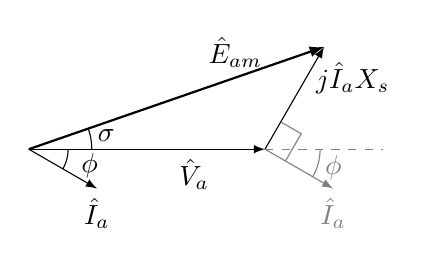
\begin{tikzpicture}
%grid
%\draw[gray,thick] (-2,-2) grid (5,2);
%\draw[gray,thin,xstep=0.1,ystep=0.1] (-2,-2) grid (5,2);
%
\draw[-latex](0,0)--(3,0)node[below,pos=0.7]{$\hat{V}_a$}coordinate(vEnd);
\draw[-latex](0,0)--++(-30:1)node[below]{$\hat{I}_a$};
\draw[] (0:0.5) arc (0:-30:0.5);
\draw[] (-15:0.8) node {$\phi$};
%
\draw[gray,-latex](vEnd)--++(-30:1)node[below]{$\hat{I}_a$};
\draw[-latex](vEnd)--++(60:1.5)coordinate(vTip)node[right,pos=0.7]{$j \hat{I}_a X_s$};
\draw[-latex,thick](0,0)--(vTip)node[above,pos=0.7]{$\hat{E}_{am}$};
\draw[gray] (vEnd)++(-30:0.3)--++(60:0.4)--++(150:0.3);
\draw[gray,dashed](vEnd)--++(0:1.5);
\draw[gray](vEnd)++(-30:0.7) arc (-30:0:0.7);
\draw[gray](vEnd)++(-15:0.9)node {$\phi$};
\draw (0.8,0) arc (0:19:0.8);
\draw (10:1) node{$\sigma$};
\end{tikzpicture}
\caption{}
\end{subfigure}%
\begin{subfigure}{0.45\textwidth}
\centering
\begin{tikzpicture}
\draw[-latex](0,0)--(3,0)node[below,pos=0.7]{$\hat{V}_a$}coordinate(vEnd);
\draw[-latex](0,0)--++(60:1)node[left]{$\hat{I}_a$};
\draw[] (0:0.5) arc (0:60:0.5);
\draw[] (45:0.7) node {$\phi$};
\draw[gray,-latex](vEnd)--++(60:1)node[right]{$\hat{I}_a$};
\draw[-latex](vEnd)--++(150:1.5)coordinate(vTip)node[shift={(0:1)}]{$j \hat{I}_a X_s$};
\draw[-latex,thick](0,0)--(vTip)node[shift={(160:0.6)}]{$\hat{E}_{am}$};
\draw[gray] (vEnd)++(60:0.3)--++(150:0.4)--++(-120:0.3);
\draw[gray,dashed](vEnd)--++(0:1);
\draw[gray](vEnd)++(0:0.4) arc (0:60:0.4);
\draw[gray](vEnd)++(30:0.6)node {$\phi$};
\draw (0.8,0) arc (0:23:0.8);
\draw (11:1) node{$\sigma$};
\end{tikzpicture}
\caption{}
\end{subfigure}%
\caption{معاصر جنریٹر کا دوری سمتیہ۔}
\label{شکل_معاصر_جنریٹر_دوری_سمتیہ}
\end{figure}

 شکل \حوالہ{شکل_معاصر_جنریٹر_کے_سادہ_مساوی_دور}-ب میں طاقت \عددیء{p_v} بائیں سے دائیں منتقل ہو رہی ہے:
\begin{align}\label{مساوات_معاصر_طاقت_کی_منتقلی_الف}
p_v=V_a I_a \cos \phi
\end{align}
مساوات \حوالہ{مساوات_معاصر_جنریٹر_دوری_سمتیہ_مساوات_سادہ} اور شکل \حوالہ{شکل_معاصر_جنریٹر_دوری_سمتیہ}-ا  سے درج ذیل لکھا جا سکتا ہے۔
\begin{gather}
\begin{aligned}\label{مساوات_معاصر_رو_بالمقابل_دو_دباو}
\hat{I}_a=I_a \phase{\phi}&=\frac{\hat{E}_{am}-\hat{V}_a}{j X_s}\\
&=\frac{E_{am} \phase{\sigma} -V_a \phase {0}}{X_s \phase{\frac{\pi}{2}}}\\
&=\frac{E_{am}}{X_s} \phase{\sigma-\frac{\pi}{2}} -\frac{V_a}{X_s} \phase {-\frac{\pi}{2}}
\end{aligned}
\end{gather}
شکل \حوالہ{شکل_معاصر_جنریٹر_دوری_سمتیہ} سے واضح ہے کہ درج بالا مساوات میں \عددی{\hat{I}_a} کا حقیقی جزو  \عددیء{\hat{V}_a} کا ہم قدم ہو گا۔کسی بھی  دوری سمتیہ \عددی{K\phase{\alpha}} کو  حقیقی افقی جزو \عددی{K\cos\alpha} اور فرضی عمودی جزو \عددی{jK\sin\alpha} کا مجموعہ تصور کیا جا سکتا ہے۔ مساوات \حوالہ{مساوات_معاصر_رو_بالمقابل_دو_دباو} کے آخری قدم میں دائیں ہاتھ کے حقیقی اجزاء سے رو کا حقیقی جزو حاصل ہو گا :
\begin{gather}
\begin{aligned}
I_a \cos \phi&=\frac{E_{am}}{X_s} \cos \left(\sigma -\frac{\pi}{2} \right)-\frac{V_a}{X_s} \cos \left(-\frac{\pi}{2} \right)\\
&=\frac{E_{am}}{X_s} \sin \sigma
\end{aligned}
\end{gather}
اس کو مساوات \حوالہ{مساوات_معاصر_طاقت_کی_منتقلی_الف}  کے ساتھ ملا کر درج ذیل ملتا ہے۔
\begin{align}\label{مساوات_معاصر_سائن_خصوصیات}
p_v=\frac{V_a E_{am}}{X_s} \sin \sigma
\end{align}
تین دوری معاصر مشین کے لئے اس مساوات کو تین سے ضرب کرنا ہو گا:
\begin{align}\label{مساوات_معاصر_طاقت_بالمقابل_زاویہ}
p_v=\frac{3 V_a E_{am}}{X_s} \sin \sigma
\end{align}
مساوات \حوالہ{مساوات_معاصر_طاقت_بالمقابل_زاویہ} طاقت بالمقابل زاویہ\فرہنگ{طاقت بالمقابل زاویہ}\حاشیہب{power-angle law}\فرہنگ{power-angle law} کا قانون پیش کرتی ہے۔اٹل \عددیء{V_a} کی صورت میں جنریٹر \عددیء{E_{am}} یا (اور) \عددیء{\sigma} بڑھا کر طاقت بڑھا سکتا ہے۔گھومتے میدانی لچھے میں برقی رو بڑھا کر  \عددیء{E_{am}} بڑھایا جاتا ہے جو ایک حد تک کرنا ممکن ہو گا چونکہ میدانی  لچھے کی مزاحمت میں برقی توانائی ضائع ہونے سے لچھا گرم ہو گا جس کو خطرناک حد تک پہنچنے نہیں دیا جا سکتا ہے۔اسی طرح  \عددیء{\sigma} کو نوے زاویہ تک بڑھایا  جا سکتا ہے جس پر، کسی مخصوص \عددی{E_{am}} کے لئے، جنریٹر زیادہ سے زیادہ طاقت مہیا کرے گا:
\begin{align}\label{مساوات_معاصر_طاقت_انتہا}
p_{v,\textup{انتہا}}=\frac{3 V_a E_{am}}{X_s}&& (\sin 90^{\circ}=1)
\end{align}
حقیقت میں جنریٹر کی بناوٹ یوں کی جاتی ہے کہ  بناوٹی (قابل استعمال) طاقت نوے درجے سے کافی کم زاویہ پر ممکن ہو۔ نوے درجے پر جنریٹر کو قابو رکھنا مشکل ہوتا ہے۔
%
\begin{figure}
\centering
%\includegraphics{figSynchronousGeneratorConnectedToMotor}
\begin{subfigure}{0.45\textwidth}
\centering
\begin{tikzpicture}
\draw(0,0) to [short,o-,i={$\hat{I}_a$}] ++(0.5,0) to [inductor,l={$j X_{sm}$}]++(2,0) to [sinusoidal voltage source] ++(0,-2) to [short,-o] (0,-2);
\draw node at (3.5,-1){$
\begin{aligned}
&+\\
&{E}_{am}\\
&-
\end{aligned}$};
\draw node at (0,-1){$\begin{aligned}
&+\\
&\hat{V}_a\\
&-
\end{aligned} $};
\end{tikzpicture}
\caption{}
\end{subfigure}%
\begin{subfigure}{0.45\textwidth}
\centering
\begin{tikzpicture}
\draw[gray,thick,-latex](0,0)--++(0:1)node[above]{$\hat{I}_a$};
\draw[-latex](0,0)--++(0:3)node[above,pos=0.8]{$\hat{V}_a$}coordinate(vTip);
\draw[latex-](vTip)--++(-90:1.5)node[pos=0.5,right]{$j \hat{I}_aX_{sm}$}coordinate(ixStart);
\draw[-latex,thick](0,0)--(ixStart)node[below,pos=0.6]{$\hat{E}_{am,m}$};
\end{tikzpicture}
\caption{}
\end{subfigure}
\begin{subfigure}{1\textwidth}
\centering
\begin{tikzpicture}
\draw(0,0) to [sinusoidal voltage source] ++(0,2) to [inductor,l={$j X_{sg}$}]++(2,0) to [short,i={$\hat{I}_a$}] ++(0.5,0) to [inductor,l={$j X_{sm}$}] ++(2,0) to [sinusoidal voltage source]++(0,-2) to (0,0);
\draw node at (2.25,1){$\begin{aligned}
&+\\
&\hat{V}_a\\
&-
\end{aligned} $};
\draw node at (-1,1){$\begin{aligned}
&+\\
&\hat{E}_{am,g}\\
&-
\end{aligned} $};
\draw node at (5.5,1){$\begin{aligned}
&+\\
&\hat{E}_{am,m}\\
&-
\end{aligned} $};
\end{tikzpicture}
\caption{}
\end{subfigure}
\begin{subfigure}{0.45\textwidth}
\centering
\begin{tikzpicture}
\pgfmathsetmacro{\Em}{2}
\pgfmathsetmacro{\Eg}{1686/1632*\Em}
\pgfmathsetmacro{\angM}{-35.548}
\pgfmathsetmacro{\angG}{38.047}
\draw[gray,thick,-latex](0,0)--++(0:1)node[above]{$\hat{I}_a$};
\draw[-latex,thick](0,0)--++(\angM:\Em)coordinate(kL)node[pos=0.75,below left]{$\hat{E}_{am,a}$};
\draw[-latex,thick](0,0)--++(\angG:\Eg)coordinate(kT)node[pos=0.75,above left]{$\hat{E}_{am,g}$};
\path(kL)--(kT)coordinate[pos=0.4773](kV)coordinate[pos=1](kE);
\draw[-latex](kL)--(kV)node[pos=0.5,right]{$j\hat{I}_aX_{sm}$};
\draw[-latex](kV)--(kE)node[pos=0.5,right]{$j\hat{I}_aX_{sg}$};
\draw[-latex](0,0)--(kV)node[pos=0.75,below]{$\hat{V}_a$};
\end{tikzpicture}
\caption{}
\end{subfigure}%
\begin{subfigure}{0.45\textwidth}
\centering
\begin{tikzpicture}
\pgfmathsetmacro{\Em}{2}
\pgfmathsetmacro{\Eg}{1686/1632*\Em}
\pgfmathsetmacro{\ang}{-43.327}
\pgfmathsetmacro{\angA}{90-43.327+\ang}
\draw[-latex,thick](0,0)--++(\ang:\Em)coordinate(kL)node[pos=0.75,below left]{$\hat{E}_{am,a}$};
\draw[-latex,thick](0,0)--++(90+\ang:\Eg)coordinate(kT)node[pos=0.75,above left]{$\hat{E}_{am,g}$};
\path(kL)--(kT)coordinate[pos=0.4773](kV)coordinate[pos=1](kE);
\draw[-latex](kL)--(kV)node[pos=0.5,right]{$j\hat{I}_aX_{sm}$};
\draw[-latex](kV)--(kE)node[pos=0.5,right]{$j\hat{I}_aX_{sg}$};
\draw[-latex](0,0)--(kV)node[pos=0.75,below]{$\hat{V}_a$};
\draw[-latex,gray](0,0)--++(\angA:1.25)node[above,xshift=-1ex]{$I_a$};
\draw(kL)++(0,0.3) arc (90:90+45:0.3);
\draw(kL)++(-0.25,0.5)node[]{$\alpha$};
\end{tikzpicture}
\caption{}
\end{subfigure}
\caption{معاصر جنریٹر معاصر موٹر چلا رہا ہے۔}
\label{شکل_معاصر_جنریٹر_موٹر_چلاتا_ہوا}
\end{figure}

\ابتدا{مثال}
ایک \عددیء{50} قطبی، ستارہ، تین دوری \عددیء{50} ہرٹز، \عددیء{2300} وولٹ دباو تار  پر چلنے والی \عددیء{1800} کلو وولٹ-ایمپیئر  معاصر مشین کا یک دوری  معاصر امالہ \عددیء{2.1} اوہم ہے۔
\begin{itemize}
\item
مشین کے برقی سروں پر \عددیء{2300} وولٹ دباو تار مہیا کیا جاتا ہے جبکہ اس کا میدانی برقی رو اتنا رکھا جاتا ہے کہ پورے بوجھ پر مشین کا جزو طاقت ایک کے برابر ہو۔ اس مشین سے زیادہ سے زیادہ کتنی قوت مروڑ حاصل کی جا سکتی ہے؟
\item
اس موٹر کو  \عددیء{2}  قطبی،  \عددیء{3000} چکر فی منٹ، تین دوری، ستارہ،  \عددیء{2300} وولٹ دباو تار پیدا کرنے والا \عددیء{2200}  کلو وولٹ-ایمپیئر کے معاصر جنریٹر سے چلایا جاتا ہے جس کا یک دوری معاصر امالہ \عددیء{2.3} اوہم ہے۔موٹر پر اس کا پورا برقی بوجھ لاد  کر جنریٹر کو معاصر رفتار پر چلاتے ہوئے دونوں مشینوں کے میدانی برقی رو تبدیل کیے جاتے ہیں حتیٰ کہ موٹر ایک جزو طاقت پر چلنے لگے۔دونوں مشینوں کا میدانی برقی رو یہاں برقرار رکھ کر موٹر پر بوجھ آہستہ آہستہ بڑھایا جاتا ہے۔اس صورت میں موٹر سے زیادہ سے زیادہ کتنی قوت مروڑ  حاصل کی جا سکتی ہے اور اس کی سروں پر دباو تار کتنا ہو گا؟ 
\end{itemize}

حل:
\begin{itemize}
\item
شکل \حوالہ{شکل_معاصر_جنریٹر_موٹر_چلاتا_ہوا}-ا اور \حوالہ{شکل_معاصر_جنریٹر_موٹر_چلاتا_ہوا}-ب سے رجوع کریں۔یک دوری برقی دباو اور کل برقی رو درج ذیل ہوں گے۔
\begin{align*}
\frac{2300}{\sqrt{3}}=\SI{1327.9}{\volt}\\
\frac{\num{1800000}}{\sqrt{3} \times 2300}=\SI{451.84}{\ampere}
\end{align*}
یوں درج ذیل ہو گا۔
\begin{align*}
\hat{E}_{am,m}&=\hat{V}_a-j \hat{I}_a X_{s,m}\\
&=1327.9 \phase {0\degree} -j 451.84 \phase {0\degree} \times 2.1\\
&=1327.9-j 948.864\\
&=1632 \phase{-35.548\degree}
\end{align*}
مساوات \حوالہ{مساوات_معاصر_طاقت_انتہا}  سے یک دوری زیادہ سے زیادہ برقی طاقت حاصل کرتے ہیں۔
\begin{align*}
p_{\textup{انتہا}}=\frac{1327.9 \times 1632}{2.1}=\SI{1031968}{\watt}
\end{align*}
اس طرح  تین دوری زیادہ سے زیادہ طاقت \عددیء{\num{3095904}} واٹ ہو گی۔\عددیء{50} ہرٹز اور \عددیء{50} قطب سے مشین کی معاصر میکانی رفتار مساوات \حوالہ{مساوات_گھومتے_مشین_برقی_میکانی_رفتار_تعلق}  کی مدد سے دو چکر فی سیکنڈ حاصل ہوتی ہے یعنی \عددیء{f_m=2}۔یوں مشین سے درج ذیل زیادہ سے زیادہ قوت مروڑ حاصل کی جا سکتی ہے۔
\begin{align*}
T_{\textup{انتہا}}=\frac{p_{\textup{انتہا}}}{2 \pi f_m}=\frac{3095904}{2 \times \pi \times 2}=\SI{246364}{\newton \meter}
\end{align*}
موٹر پر اس سے زیادہ قوت مروڑ کا بوجھ مسلط کرنے سے موٹر  رک جائے گی جبکہ جنریٹر کی رفتار بے قابو بڑھنے شروع ہو جائے گی۔ خود کار منقطع کار  اس لمحہ پر نظام کو روک دیگا۔
\item
شکل \حوالہ{شکل_معاصر_جنریٹر_موٹر_چلاتا_ہوا}-ج سے رجوع کریں۔اس مثال کے پہلے جزو کی طرح یہاں بھی موٹر کے برقی سروں پر دباو تار  \عددیء{2300} وولٹ اور  محرک برقی دباو \عددیء{1632} وولٹ ہوں گے۔ جنریٹر کا محرک برقی دباو درج ذیل ہو گا۔
\begin{align*}
\hat{E}_{am,g}&=\hat{V}_a+j  \hat{I}_a X_{s,g}\\
&=1327.9 \phase {0\degree} +j 451.84 \phase {0\degree} \times 2.3\\
&=1327.9+j 1039.233\\
&=1686 \phase{38.047\degree}
\end{align*}
یہ صورت شکل \حوالہ{شکل_معاصر_جنریٹر_موٹر_چلاتا_ہوا}-د میں دکھائی گئی ہے۔

جیسا شکل \حوالہ{شکل_معاصر_جنریٹر_موٹر_چلاتا_ہوا}-ھ میں دکھایا گیا ہے، موٹر اس  وقت زیادہ سے زیادہ طاقت پیدا کرے گی جب  \عددیء{\hat{E}_{am,g}} اور \عددیء{\hat{E}_{am,m}} آپس میں \عددیء{90\degree} زاویہ پر ہوں۔

یہاں  مساوات \حوالہ{مساوات_معاصر_طاقت_انتہا}  میں ایک معاصر امالہ کی بجائے موٹر اور جنریٹر کے  سلسلہ وار جڑے امالہ ہوں گے  اور دو برقی دباو اب موٹر اور جنریٹر کے محرک برقی دباو ہوں گے۔یوں موٹر کی یک دوری  زیادہ سے زیادہ طاقت درج ذیل ہو گی۔
\begin{align*}
p_{\textup{انتہا}}=\frac{1686 \times 1632}{2.3+2.1}=\SI{625352}{\watt}
\end{align*}	
اس طرح تین دوری طاقت  \عددیء{\num{1876056 }} واٹ  اور زیادہ سے زیادہ قوت مروڑ درج ذیل ہو گی۔
\begin{align*}
T_{\textup{انتہا}}=\frac{1876056}{2 \times \pi \times 2}=\SI{149291}{\newton \meter}
\end{align*}
\end{itemize}
شکل \حوالہ{شکل_معاصر_جنریٹر_موٹر_چلاتا_ہوا}-ھ میں \عددی{\hat{E}_{am,m}} اور \عددی{\hat{E}_{am,g}} آپس میں عمودی ہیں لہٰذا درج ذیل ہو گا۔
\begin{align*}
I_a(X_{s,g}+X_{s,m})&=\sqrt{E^2_{am,m}+E^2_{am,g}}=\SI{2346}{\volt}\\
I_a&=\frac{2346}{2.1+2.3}=\SI{533}{\ampere}\\
I_aX_{sg}&=533\times 2.1=\SI{1119.9}{\volt}\\
\alpha&=\tan^{-1}\frac{1686}{1632}=45.93^{\circ}
\end{align*} 
یوں دوری دباو \عددی{V_a}، جو صفر زاویہ پر تصور کیا جاتا ہے،  درج ذیل ہو گا۔
\begin{align*}
V_a=\sqrt{1632^2+1119.9^2-2\times 1632\times1119.9\times\cos 45.93^{\circ}}=\SI{1172.7}{\volt}
\end{align*}
لامتناہی نظام کی بجائے موٹر کو جنریٹر سے طاقت مہیا کر کے، موٹر پر بوجھ بڑھانے  سے موٹر کے سروں پر برقی دباو گھٹتا ہے جس کی بنا زیادہ سے زیادہ ممکنہ طاقت \عددی{\SI{3095}{\kilo\watt}} سے گھٹ کر \عددی{\SI{1876}{\kilo\watt}} رہ گئی ہے۔ موٹر کی سروں پر برقی دباو  \عددی{\hat{V}_a} اور برقی رو \عددی{\hat{I}_a} ہم قدم نہیں ہیں۔ 
\انتہا{مثال}
%
\حصہ{یکساں حال، برقرار چالو مشین کے خواص}
\جزوحصہ{معاصر جنریٹر: برقی بوجھ بالمقابل \عددیء{I_m} کے خط}
شکل \حوالہ{شکل_معاصر_جنریٹر_کے_سادہ_مساوی_دور}-ب کی دوری سمتیہ  مساوات
\begin{align}\label{مساوات_معاصر_دوری_جنریٹر_مساوات}
\hat{E}_{am}=\hat{V}_a+j \hat{I}_a X_s
\end{align}
میں \عددی{\hat{I}_a=I_a\phase{\phi}} لیتے ہوئے درج ذیل لکھا جا سکتا ہے
\begin{align}
E_{am}\phase{\sigma}=V_a \phase{0} +I_a X_s \phase{\frac{\pi}{2}+\phi}
\end{align}
جس کو بطور مخلوط عدد\فرہنگ{مخلوط عدد}\حاشیہب{complex number}
\begin{small}
\begin{align*}
E_{am} \cos \sigma +j E_{am} \sin \sigma&=V_a \cos 0+j V_a \sin 0 + I_a X_s \cos \left(\frac{\pi}{2}+\phi \right)+j I_a X_s \sin \left(\frac{\pi}{2}+\phi \right)\\
&=E_{am,x}+j E_{am,y}
\end{align*}
\end{small}
لکھ سکتے ہیں۔ اس  سے \عددیء{\abs{\hat{E}_{am}}} یعنی  \عددیء{E_{am}}  حاصل کرتے ہیں۔
\begin{gather}
\begin{aligned}\label{مساوات_معاصر_رو_بالمقابل_دباو}
\abs{\hat{E}_{am}}=E_{am}&=\sqrt{E_{am,x}^2+E_{am,y}^2}\\
&=\sqrt{V_a^2+\left(I_a X_s\right)^2 +2 V_a I_a X_s \sin \phi}
\end{aligned}
\end{gather}
جنریٹر کے سروں پر  \عددیء{V_a} اٹل رکھتے ہوئے مختلف \عددیء{\phi} کے لئے \عددیء{E_{am}} بالمقابل \عددیء{I_a} کے خط شکل \حوالہ{شکل_معاصر_بار_بالمقابل_میدانی_رو}  میں دکھائے گئے ہیں۔یہ خطوط مساوات \حوالہ{مساوات_معاصر_رو_بالمقابل_دباو} دیتی ہے۔ چونکہ \عددیء{E_{am}}  اور  \عددیء{I_m}  راست متناسب ہیں اور کسی  مخصوص جزو طاقت اور معین \عددیء{V_a} کے لئے جنریٹر کی طاقت \عددیء{I_a} کے   راست متناسب ہوتی ہے لہٰذا یہی ترسیمات \عددیء{I_m} بالمقابل جنریٹر کی طاقت کو بھی ظاہر کرتی ہیں۔
\begin{figure}
\centering
%\includegraphics{figSynchronousCompoundingCurves}
\begin{tikzpicture}
\begin{axis}[
	ticks=none,
	xmin=0,
	xmax=1.35,
	ymin=0,
%	axis lines=middle,
%	axis y line=middle,
	axis line style=-,
%	ytick={0.25,0.5},
%	yticklabels={50,100},
%	xtick style={draw=none},
	ylabel style={align=right},
	ylabel={\RL{ $V_a$ برقرار رکھنے کے لئے} \\ \RL{ درکار میدانی برقی رو $I_m$}},
	xlabel style={align=right},
	xlabel={\RL{برقی بار یا قوی لچھے کا برقی رو $I_a$}},
]
\newcommand\tka{0}
\addplot[
black,
domain=0:1.1,
samples=100,
]
{sqrt(1+x*x+2*x*sin(\tka))} node[right] {\RL{ہم قدم}} ;
%==
\newcommand\tkb{36}
\addplot[
black,
domain=0:1.1,
samples=100,
]
{sqrt(1+x*x+2*x*sin(\tkb))} node[right] {پیچھے} ;
%=====
\newcommand\tkc{-36}
\addplot[
black,
domain=0:1.1,
samples=100,
]
{sqrt(1+x*x+2*x*sin(\tkc))} node[right] {آگے} ;
\addplot[dashed]coordinates {(1,0)(1,2)}node[pos=0.2,left]{\RL{پورا بوجھ}};
\end{axis}
\end{tikzpicture}
\caption{جنریٹر: برقی بوجھ بالمقابل \عددیء{I_m} کے خط}
\label{شکل_معاصر_بار_بالمقابل_میدانی_رو}
\end{figure}
\جزوحصہ{معاصر موٹر:\عددیء{I_a}   بالمقابل \عددیء{I_m}  کے خط}
معاصر موٹر کا مساوی دور (ریاضی نمونہ) شکل \حوالہ{شکل_معاصر_موٹر_کا_مساوی_دور}   اور دوری سمتیہ شکل  \حوالہ{شکل_معاصر_موٹر_کی_دوری_سمتیہ} میں دکھایا گیا ہے۔  مزاحمت نظرانداز کر کے اس کی مساوات لکھتے ہیں۔
\begin{gather}
\begin{aligned}
\hat{V}_a&=\hat{E}_{am}+j \hat{I}_a X_s\\
V_a \phase{0}&=E_{am} \phase{\sigma} +j I_a \phase{\phi} X_s\\
&=E_{am} \phase{\sigma} +I_a X_s \phase{\frac{\pi}{2}+\phi}
\end{aligned}
\end{gather}
اس مساوات میں موٹر پر لاگو برقی دباو \عددیء{\hat{V}_a} کے حوالہ سے زاویات کی پیمائش کی گئی ہے لہٰذا  \عددیء{\hat{V}_a}  کا زاویہ صفر ہو گا۔یاد رہے کہ مثبت زاویہ کی پیمائش افقی لکیر سے گھڑی کے مخالف رخ ہو گی  لہٰذا \اصطلاح{پیش} زاویہ\حاشیہب{leading angle} مثبت اور \اصطلاح{تاخیری} زاویہ\حاشیہب{lagging angle} منفی ہو گا۔ اس مساوات سے امالی دباو \عددیء{E_{am}}  حاصل کرتے ہیں۔
\begin{align*}
E_{am}\phase{\sigma}&=V_a \phase{0}-I_a X_s \phase{\frac{\pi}{2}+\phi}\\
&=V_a -I_a X_s  \cos \left( \frac{\pi}{2}+\phi\right)- j I_a X_s \sin \left(\frac{\pi}{2}+\phi \right)\\
&=V_a +I_a X_s \sin \phi-j I_a X_s \cos \phi
\end{align*}
یوں \عددی{\abs{E_{am}}} درج ذیل ہو گا۔
\begin{gather}
\begin{aligned}\label{مسوات_معاصر_دوری_مساوات}
\abs{E_{am}}&=\sqrt{\left(V_a +I_a X_s \sin \phi \right)^2+\left(I_a X_s \cos \phi \right)^2}\\
&=\sqrt{V_a^2+I_a^2 X_s^2+ 2 V_a I_a X_s \sin \phi}
\end{aligned}
\end{gather}
موٹر پر لاگو برقی دباو اور اس پر میکانی بوجھ کو \عددیء{\SI{0}{\percent}}، \عددیء{\SI{25}{\percent}} اور \عددیء{\SI{75}{\percent}} پر رکھ کر، موٹر کے \عددیء{E_{am}} بالمقابل  \عددیء{I_a} خطوط،  مساوات \حوالہ{مسوات_معاصر_دوری_مساوات} سے  شکل \حوالہ{شکل_معاصر_برقی_رو_بالمقابل_برقی_دباو}   میں  ترسیم کیے گئے ہیں۔ چونکہ امالی دباو \عددیء{I_m} کا راست متناسب ہوتا ہے  لہٰذا یہی موٹر کے \عددیء{I_m} بالمقابل \عددیء{I_a} خطوط بھی ہوں گے۔ان میں سے ہر خط ایک معین میکانی بوجھ \عددیء{p} کے لئے ہے جہاں \عددی{p} درج ذیل ہو گا۔
\begin{align}\label{مساوات_معاصر_طاقت_برابر_دباو_رو_جزو_طاقت}
p=V_a I_a \cos \phi
\end{align}
%
\begin{figure}
\centering
%\includegraphics{figSynchronousMotorPhasorDiagram}
\begin{subfigure}{0.45\textwidth}
\centering
\begin{tikzpicture}
\pgfmathsetmacro{\phaseI}{-45}
\pgfmathsetmacro{\phaseV}{0}
\draw[thick,-latex](0,0)--++(\phaseI:1.5)node[left]{$\hat{I}_a$};
\draw[-latex](0,0)--++(\phaseV:3)node[above,pos=0.8]{$\hat{V}_{s}$}coordinate(vTip);
\draw[latex-](vTip)--++(-90+\phaseI:1.5)node[pos=0.5,right]{$j \hat{I}_aX_{s}$}coordinate(ixStart);
\draw[-latex,thick](0,0)--(ixStart)node[below]{$\hat{E}_{am}$};
%text
\draw[](0:0.6) arc (0:\phaseI:0.6);
\draw[](-13:0.85)node{$\phi$};
%
\draw(0:1.2) arc (0:-28:1.2);
\draw(-14:1.4)node{$\sigma$};
\draw node[right] at (0,1.5){\RL{برقی رو پیچھے ہے}};
\end{tikzpicture}
\caption{}
\end{subfigure}%
\begin{subfigure}{0.45\textwidth}
\centering
\begin{tikzpicture}
\pgfmathsetmacro{\phaseI}{45}
\pgfmathsetmacro{\phaseV}{0}
\draw[thick,-latex](0,0)--++(\phaseI:1.5)node[above left]{$\hat{I}_a$};
\draw[-latex](0,0)--++(\phaseV:3)node[above,pos=0.8]{$\hat{V}_{s}$}coordinate(vTip);
\draw[latex-](vTip)--++(-90+\phaseI:1.5)node[pos=0.5,above right]{$j \hat{I}_aX_{s}$}coordinate(ixStart);
\draw[-latex,thick](0,0)--(ixStart)node[below,pos=0.7]{$\hat{E}_{am}$};
%text
\draw[](0:0.6) arc (0:\phaseI:0.6);
\draw[](22.5:0.85)node{$\phi$};
%
\draw(0:1.2) arc (0:-14:1.2);
\draw(-7:1.4)node{$\sigma$};
\draw node[right] at (2,1.5){\RL{برقی رو آگے ہے}};
\end{tikzpicture}
\caption{}
\end{subfigure}%
\caption{موٹر کا دوری سمتیہ۔}
\label{شکل_معاصر_موٹر_کی_دوری_سمتیہ}
\end{figure}
%
\begin{figure}
\centering
%\includegraphics{figSynchronousVcurves}
\begin{tikzpicture}
\begin{axis}[
	ticks=none,
%	xmin=0,
%	xmax=1.35,
	ymin=0,
%	axis lines=middle,
%	axis y line=middle,
	axis line style=-,
%	ytick={0.25,0.5},
%	yticklabels={50,100},
%	xtick style={draw=none},
	ylabel style={align=right},
	ylabel={\RL{قوی لچھے کا برقی رو $I_a$}},
	xlabel style={align=right},
	xlabel={\RL{میدانی لچھے کا برقی رو $I_m$}},
]
%
\def\p{0}
\addplot[black,domain=\p*100:101,samples=100,]({sqrt(1+x/100*x/100-2*sqrt(x/100*x/100-\p*\p))},{x}) node [above]{$\SI{0}{\percent}$} ;
\addplot[black,domain=\p*100:101,samples=100,]({sqrt(1+x/100*x/100+2*sqrt(x/100*x/100-\p*\p))},{x}) ;   %}
%
\def\p{0.25}
\addplot[black,domain=\p*100:101,samples=100,]({sqrt(1+x/100*x/100-2*sqrt(x/100*x/100-\p*\p))},{x}) node [right]{$\SI{25}{\percent}$} ;
\addplot[black,domain=\p*100:101,samples=100,]({sqrt(1+x/100*x/100+2*sqrt(x/100*x/100-\p*\p))},{x}) ; 
%
\def\p{0.75}
\addplot[black,domain=\p*100:101,samples=100,]({sqrt(1+x/100*x/100-2*sqrt(x/100*x/100-\p*\p))},{x}) node [right]{$\SI{75}{\percent}$} ;
\addplot[black,domain=\p*100:101,samples=100,]({sqrt(1+x/100*x/100+2*sqrt(x/100*x/100-\p*\p))},{x}) ; 
\end{axis}
\end{tikzpicture}
\caption{موٹر کی $I_{m}$ بالمقابل $I_a$ ترسیم۔}
\label{شکل_معاصر_برقی_رو_بالمقابل_برقی_دباو}
\end{figure}

اس مساوات کے تحت  \عددیء{p} اور \عددیء{V_a} تبدیل کیے بغیر  جزو طاقت تبدیل کر کے \عددیء{I_a} تبدیل کیا جا سکتا ہے۔ شکل \حوالہ{شکل_معاصر_برقی_رو_بالمقابل_برقی_دباو} کے حصول میں  مساوت \حوالہ{مسوات_معاصر_دوری_مساوات}  کو مساوات \حوالہ{مساوات_معاصر_طاقت_برابر_دباو_رو_جزو_طاقت}  کی مدد سے ترسیم کیا جاتا ہے۔مخصوص \عددیء{V_a} اور \عددیء{p} کے لئے مختلف \عددیء{I_a} پر مساوات \حوالہ{مساوات_معاصر_طاقت_برابر_دباو_رو_جزو_طاقت}   سے \عددیء{\phi} حاصل کیا جاتا ہے۔اس کے بعد  ہر انفرادی \عددیء{I_a} اور  مطابقتی  \عددیء{\phi}  کو مساوات  \حوالہ{مسوات_معاصر_دوری_مساوات} میں پر  کر کے \عددیء{E_{am}} حاصل کیا جاتا ہے۔ مخصوص \عددی{p} کے لئے   \عددیء{E_{am}} بالمقابل \عددیء{I_a} ترسیم کیے جاتے ہیں۔ شکل \حوالہ{شکل_معاصر_برقی_رو_بالمقابل_برقی_دباو} میں \عددی{\SI{0}{\percent}}، \عددی{\SI{25}{\percent}} اور \عددی{\SI{75}{\percent}} طاقت کے لئے ترسیمات پیش کی گئی ہیں۔

موٹر کے خطوط سے واضح ہے کہ \عددیء{I_m}  تبدیل کر کے موٹر کا جزو طاقت تبدیل کیا جا سکتا ہے۔ یوں موٹر کو \اصطلاح{پیش} زاویہ یا \اصطلاح{تاخیری} زاویہ  پر چلایا جا سکتا ہے۔ موٹر کو پیش زاویہ چلا کر بطور ایک \اصطلاح{برق گھیر}\فرہنگ{برق گھیر}\حاشیہب{capacitor}\فرہنگ{capacitor}  استعمال کیا جا  سکتا ہے۔ حقیقت میں ایسا نہیں کیا جاتا ہے چونکہ معاصر موٹر سے برق گھیر زیادہ سستا دستیاب ہوتا ہے۔ 

\حصہ{کھلا دور  اور کسر دور  معائنہ}
معاصر مشین کا مساوی دور بنانے کے لئے مساوی دور کے اجزاء جاننا لازم ہے جنہیں دو قسم کے معائنوں سے معلوم کیا جاتا ہے۔ انہیں کھلا دور معائنہ اور کسر دور معائنہ کہتے ہیں۔ان معائنوں سے قالب کے سیرابیت کے اثرات بھی اجاگر ہوتے ہیں۔اسی قسم کے معائنے ٹرانسفارمر کے  بھی کیے جاتے ہیں جہاں  کھلا دور معائنہ ٹرانسفارمر کے بناوٹی  برقی دباو جبکہ کسر دور معائنہ بناوٹی  برقی رو پر کیا جاتا ہے۔یہاں بھی ایسا کیا جائے گا۔ 

\جزوحصہ{کھلا دور معائنہ}
معاصر مشین کے برقی سرے کھلا رکھ کر، مشین کو معاصر رفتار پر گھماتے ہوئے مختلف \عددیء{I_m} پر پیدا برقی دباو \عددیء{V_a}  مشین کے سروں پر  ناپا جاتا ہے ۔ان کی  رو \عددی{I_m} بالمقابل دباو \عددی{V_a}  ترسیم شکل \حوالہ{شکل_معاصر_کھلے_دور_خط}-ا میں دی گیا ہے۔ یہ ترسیم مشین کی کھلا دور خاصیت ظاہر کرتی ہے۔ یہ ترسیم مشین بنانے والے بھی مہیا کر سکتے ہیں۔

اس کتاب کے حصہ \حوالہ{حصہ_مقناطیسی_دور_مقناطیسی_مادہ_کے_خصوصیات} میں بتایا گیا  کہ قالب پر لاگو مقناطیسی دباو بڑھانے سے قالب میں مقناطیسی بہاو بڑھتا ہے البتہ جلد ہی قالب سیراب ہو جاتا ہے۔یہ اثر  شکل-ا میں ترسیم کے جھکاو  سے واضح ہے۔قالب سیراب نہ ہونے کی صورت میں  ترسیم  نقطہ دار سیدھی لکیر کی پیروی کرتی۔مشین کا بناوٹی برقی دباو اور اس کے حصول کے لئے درکار  رو \عددیء{I_{m0}} بھی دکھائے گئے ہیں۔
\begin{figure}
\centering
%\includegraphics{figSynchronousOpenCircuitCharacteristic}
\begin{subfigure}{0.45\textwidth}
\centering
\begin{tikzpicture}
%axis
\draw[] (0,0)--(2.5,0)node[right]{$I_m$};
\draw[] (0,0)--(0,2)node[above]{$V_{a}$};
%curves
\draw[dashed] (0,0)--++(60:2.2);
\draw(0,0)--++(60:1.3) to [out=60,in=190] ++(1.4,0.75)node[below right,align=right]{\RL{قالب سیراب ہونے}\\ \RL{ کی نشانی}};
\draw[] (1.4,1.7) to [out=-45,in=180] (2,1.5);
\draw[](1.1,1.6)--(0,1.6)node[left,yshift=0.5ex]{$V_{\textup{بناوٹی}}$};
\draw node[rotate=90] at (-0.4,0.65){\RL{\small{کھلا دور برقی دباو}}};
\draw[](1.1,1.6)--(1.1,0)node[below,black]{$I_{m0}$};
\end{tikzpicture}
\caption{}
\end{subfigure}%
\begin{subfigure}{0.45\textwidth}
\centering
\begin{tikzpicture}
%axis
\draw[] (0,0)--(3,0)node[right]{$V_a$};
\draw[] node at (1.5,-0.3){\RL{کھلا دور برقی دباو}};
\draw[] (0,0)--(0,2)node[xshift=-0.35cm,rotate=90,pos=0.5]{\RL{قالبی ضیاع}};
%curves
\draw (0,0)--++(0.4,0) to [out=0,in=-115] (2.2,1.8);
\end{tikzpicture}%
\caption{}
\end{subfigure}%
\caption{کھلا دور خط اور قالبی ضیاع۔}
\label{شکل_معاصر_کھلے_دور_خط}
\end{figure}

کھلا دور معائنہ کے دوران دھرے پر  میکانی طاقت \عددیء{p_1} کی پیمائش بے بوجھ مشین کا ضیاع طاقت  دے گی۔ اس کا بیشتر حصہ رگڑی ضیاع، کچھ قالبی ضیاع  اور کچھ گھومتے لچھے کا ضیاع  ہو گا۔یاد رہے  گھومتے لچھے کو عموماً دھرے پر نسب یک سمت  جنریٹر برقی توانائی فراہم کرتا ہے جس کو از خود  طاقت محرک\حاشیہد{گھومتے لچھے کو توانائی یک سمت  جنریٹر مہیا کرتا ہے اور اس جنریٹر کو دھرے سے توانائی موصول ہوتی ہے۔} فراہم کرتا ہے۔رگڑی ضیاع کا مشین پر لدے بوجھ سے کوئی خاص تعلق نہیں پایا جاتا ہے لہٰذا  بے بوجھ مشین اور بوجھ بردار مشین  کا رگڑی ضیاع ایک جیسا تصور کیا جاتا ہے۔

رو \عددیء{I_m}  صفر رکھتے ہوئے دوبارہ دھرے پر میکانی طاقت \عددیء{p_2} کی پیمائش صرف رگڑی ضیاع دے گا۔ان پیمائشوں کا فرق  \عددیء{(p_1-p_2)} قالبی ضیاع  اور گھومتے لچھے کا برقی ضیاع  ہو گا۔گھومتے لچھے میں برقی ضیاع بہت کم ہوتا ہے اور اس کو عموماً قالب کے ضیاع کا حصہ تصور کیا جاتا ہے۔ یوں  پیمائش کردہ قالبی ضیاع کی ترسیم شکل  \حوالہ{شکل_معاصر_کھلے_دور_خط}-ب میں دی گئی ہے۔

\جزوحصہ{کسر دور معائنہ}
معاصر مشین کو معاصر رفتار پر بطور جنریٹر  چلاتے ہوئے  ساکن لچھا کسر دور کر کے مختلف \عددیء{I_m} پر کسر دور برقی رو \عددیء{I_a} ناپی جاتی ہے۔ ان کی ترسیم شکل \حوالہ{شکل_معاصر_کسر_دور_اور_کھلے_دور_خط}-ا میں دی گئی ہے جو خط کسر دور مشین کی خاصیت دکھاتی ہے۔ 

 کسر دور معائنہ کے دوران  دھیان رہے  کہ \عددیء{I_a}  خطرناک حد تک  بڑھ نہ جائے۔  جنریٹر کے بناوٹی \عددیء{I_{a}}  یا اس سے دگنی قیمت  سے رو کو  کم رکھا جاتا ہے۔ایسا نہ کرنے سے مشین گرم ہو کر تباہ ہو سکتی ہے۔

کسر دور مشین میں بناوٹی برقی دباو کے دس سے پندرہ فی صد برقی دباو پر مشین میں سو فی صد برقی رو پایا جاتا ہے۔ اتنا کم برقی دباو حاصل کرنے کے لئے خلائی درز میں اسی تناسب سے  کم مقناطیسی بہاو درکار ہو گا۔ 
\begin{figure}
\centering
%\includegraphics{figSynchronousShortCircuitCharacteristic}
\begin{subfigure}{0.45\textwidth}
\centering
\begin{tikzpicture}
%axis
\draw[] (0,0)--(1.5,0)node[right]{$I_m$};
\draw[] (0,0)--(0,2)node[above]{$I_{a }$};
\draw[] node[rotate=90] at (-1,1){\RL{کسر دور برقی رو}};
%curves
\draw (0,0)--++(60:2.2)coordinate[pos=0.7](pointE);
%
\draw[](pointE)--($(0,0)! (pointE)!(1.5,0)$)node[below,black]{$I_{m0}$};
\draw[](pointE)--($(0,0)! (pointE)!(0,2)$)node[left,black]{$I_{a0}$};
\end{tikzpicture}%
\caption{}
\end{subfigure}%
\begin{subfigure}{0.45\textwidth}
\centering
\begin{tikzpicture}
\draw[](1.1,1.6)--(1.1,0)node[below,black]{$I_{m0}$};
\draw[](1.1,1.6)--(0,1.59)node[left,black]{$V_{a0}$};
\draw[] node[rotate=90] at (-1,1){\RL{کھلا دور برقی دباو}};
%axis
\draw[] (0,0)--(2.5,0)node[right]{$I_m$};
\draw[] (0,0)--(0,2)node[above]{$V_a$};
%curves
\draw (0,0)--++(60:2.2);
\draw(0,0)++(60:1.3) to [out=60,in=190] ++(1.4,0.75);
\draw[](pointE)--($(0,0)!(pointE)!(2.5,0)$);
\end{tikzpicture}
\caption{}
\end{subfigure}%
\caption{کسر دور خط اور کھلے دور خط۔}
\label{شکل_معاصر_کسر_دور_اور_کھلے_دور_خط}
\end{figure}

شکل \حوالہ{شکل_معاصر_جنریٹر_کے_سادہ_مساوی_دور}-ا  میں جنریٹر کا مساوی برقی دور دکھایا گیا ہے جسے  شکل \حوالہ{شکل_معاصر_امالہ_معاصر}  میں کسر دور دکھایا گیا ہے۔یوں درج ذیل ہو گا۔
\begin{align}
\hat{E}_{am}=\hat{I}_a R_a+j \hat{I}_a X_s
\end{align}
\عددی{X_s>>R_a} کی بنا مزاحمت \عددیء{R_a}  نظر انداز کر کے اس مساوات سے معاصر امالہ حاصل ہو گا۔
\begin{align}\label{مساوات_معاصر_معاصر_امالہ_پیمائش}
X_s=\frac{\abs{\hat{E}_{am}}}{\abs{\hat{I}_a}}=\frac{E_{am}}{I_a}
\end{align}
%
\begin{figure}
\centering
%\includegraphics{figSynchronousReactanceSynchronous}
\begin{tikzpicture}
 \draw(0,0) to [short,o-,i={$\hat{I}_a$}] ++(1,0) to [resistor,l={$R_a$}] ++(2,0) to [inductor,l={$j X_s$}] ++(2,0) to ++(0,-2) to [short,-o] (0,-2);
\draw node at (0,-1){$
\begin{aligned}
&+\\
&\hat{E}_{am}\\
&-
\end{aligned} $};
%txt
\draw node[right] at (6,-1){$
\begin{aligned}
\hat{E}_{am}&=\hat{I}_a R_a +j \hat{I}_a X_s\\
&\approx j \hat{I}_a X_s \quad \quad \quad X_s \gg R_a\\
X_s&=\frac{|\hat{E}_{am}|}{|\hat{I}_a|}
\end{aligned}
$};
\end{tikzpicture}
\caption{معاصر امالہ۔}
\label{شکل_معاصر_امالہ_معاصر}
\end{figure}
مساوات \حوالہ{مساوات_معاصر_معاصر_امالہ_پیمائش} میں \عددیء{\hat{I}_a} کسر دور مشین کا برقی رو اور \عددیء{\hat{E}_{am}}  اسی حال میں مشین کے ایک دور کا امالی دباو ہے۔ کھلے دور مشین میں \عددیء{\hat{I}_a} صفر ہوتا ہے ۔مساوات \حوالہ{مساوات_معاصر_دوری_جنریٹر_مساوات} سے واضح ہے کہ  \عددیء{\hat{I}_a} صفر ہونے کی صورت میں \عددیء{\hat{E}_{am}}  اور \عددیء{\hat{V}_a} برابر ہوں گے۔ یوں  کسی معین \عددیء{I_{m0}} پر شکل \حوالہ{شکل_معاصر_کسر_دور_اور_کھلے_دور_خط}-ا سے  \عددیء{I_{a0}} اور شکل \حوالہ{شکل_معاصر_کسر_دور_اور_کھلے_دور_خط}-ب سے \عددیء{V_{a0}} پڑھ کر \عددیء{X_s} کی قیمت حاصل کی جا سکتی ہے۔
\begin{align}
X_s=\frac{V_{a0}}{I_{a0}}
\end{align}
معاصر امالہ کو عموماً مشین کے پورے (بناوٹی) برقی دباو پر معلوم کیا جاتا ہے تا کہ قالب کی سیرابیت کے اثرات کو بھی شامل ہو۔

مشین کو ستارہ نما تصور کر کے اس کا یک دوری \عددیء{X_s} حاصل کیا جاتا ہے۔یوں اگر معائنہ میں مشین کا تار برقی دباو\حاشیہب{line voltage} ناپا گیا ہو تب ضروری ہے کہ اس  کو \عددیء{\sqrt{3}} سے تقسیم کر کے  یک دوری  دباو حاصل کر کے مساوات \حوالہ{مساوات_معاصر_معاصر_امالہ_پیمائش} میں استعمال کیا جائے گا۔
\begin{align}
V_{\textup{یکدوری}}=\frac{V_{\textup{تار}}}{\sqrt{3}}
\end{align}
%
\ابتدا{مثال}
ایک  \عددیء{75}  کلو وولٹ-ایمپیئر، ستارہ،  \عددیء{415} وولٹ پر چلنے والی تین دوری معاصر مشین کا کھلا دور اور کسر دور معائنہ کیا گیا۔حاصل نتائج درج ذیل ہیں۔
\begin{itemize}
\item
کھلا دور معائنہ:\عددیء{V_{\textup{تار}}=\SI{415}{\volt}} اور \عددیء{I_m=\SI{3.2}{\ampere}} ہیں۔
\item
کسر دور معائنہ:
جس لمحہ قوی لچھے کا برقی رو \عددیء{\SI{104}{\ampere}} تھا اس لمحہ میدانی لچھے کا برقی رو \عددیء{\SI{2.48}{\ampere}} تھا اور جس لمحہ  قوی لچھے کا برقی رو \عددیء{\SI{126}{\ampere}} تھا اس لمحہ میدانی لچھے کا برقی رو \عددیء{\SI{3.2}{\ampere}} تھا۔
\end{itemize}
اس مشین کا معاصر امالہ تلاش کریں۔

حل: \quad
یک دوری برقی دباو درج ذیل ہو گا۔
\begin{align*}
V_{\textup{یکدوری}}=\frac{V_{\textup{تار}}}{\sqrt{3}}=\frac{415}{\sqrt{3}}=\SI{239.6}{\volt}
\end{align*}
کھلا دور مشین پر \عددی{239.6} وولٹ کے لئے   \عددیء{3.2}  ایمپیئر میدانی برقی رو درکار ہو گا جبکہ \عددی{3.2} ایمپیئر میدانی برقی رو پر کسر دور برقی رو  \عددیء{126} ایمپیئر ہو گا لہٰذا یک دوری معاصر امالہ  درج ذیل ہو گا۔
\begin{align*}
X_s=\frac{239.6}{126}=\SI{1.901}{\ohm}
\end{align*}
\انتہا{مثال}
%
کسر دور معائنہ کے دوران  دھرے پر لاگو میکانی طاقت \عددیء{p_3} کی پیمائش سے  کسر دور مشین کا کل ضیاع حاصل ہو گا۔\عددیء{p_3} ناپتے وقت کسر دور برقی رو \عددیء{I_{a,3}} بھی ناپ لیں۔اس ضیاع کا کچھ حصہ قالبی ضیاع، کچھ دونوں لچھوں میں برقی ضیاع اور کچھ رگڑی (میکانی) ضیاع ہو گا۔شکل \حوالہ{شکل_معاصر_کسر_دور_ضیاع}  میں  ضیاع طاقت بالمقابل کسر دور برقی رو  دکھایا گیا ہے۔

ضیاع \عددی{p_3} سے، کھلا دور معائنہ میں حاصل، رگڑی ضیاع \عددیء{p_2} منفی کرنے سے لچھوں کا ضیاع اور قالبی ضیاع حاصل ہو گا۔ جیسا پہلے ذکر کیا گیا، صرف دس تا بیس فی صد بناوٹی برقی دباو پر کسر دور مشین میں بناوٹی رو پایا جائے گا۔ اتنا کم برقی دباو حاصل کرنے کے لئے درکار مقناطیسی بہاو اتنا ہی کم ہو گا۔ اتنے کم مقناطیسی بہاو پر قالبی ضیاع کو نظر انداز کیا جا سکتا ہے۔ مزید ، کسر دور معاصر مشین کے گھومتے لچھے کا برقی ضیاع ساکن لچھے کے برقی ضیاع سے بہت کم ہو گا لہٰذا  گھومتے لچھے کے ضیاع کو بھی نظرانداز کیا جا سکتا ہے۔یوں \عددیء{(p_3-p_2)} کو ساکن لچھے کا برقی ضیاع تصور کیا جا سکتا ہے۔یوں درج ذیل ہو گا
\begin{align*}
p_3-p_2=I_{a,3}^2 R_a
\end{align*}
جس  سے معاصر مشین کی مساوی مزاحمت حاصل ہو گی۔
\begin{align}
R_a=\frac{p_3-p_2}{I_{a,3}^2}
\end{align}
%
\begin{figure}
\centering
%\includegraphics{figSynchronousShortCircuitedLoss}
\begin{tikzpicture}
%axis
\draw[] (0,0)--(3,0)node[right]{$ I_a$};
\draw[] node at (1.5,-0.3){\RL{کسر دور برقی رو}};
\draw[] (0,0)--(0,2)node[xshift=-0.35cm,rotate=90,pos=0.5]{\RL{ضیاع طاقت}};
%curves
\draw (0,0) to [out=0,in=-115] (2.2,1.8);
\end{tikzpicture}
\caption{کسر دور معاصر مشین میں ضیاع طاقت۔}
\label{شکل_معاصر_کسر_دور_ضیاع}
\end{figure}
\ابتدا{مثال}
ایک  \عددیء{75} کلو وولٹ-ایمپیئر،  \عددیء{415} وولٹ پر چلنے والی تین دوری معاصر مشین کے پورے (بناوٹی) برقی رو پر  کل کسر دور طاقت کا ضیاع  \عددیء{2.2} کلو واٹ ہے۔ اس مشین کی یک دوری موثر مزاحمت حاصل کریں۔

حل:\quad
یک دوری ضیاع  \عددیء{\tfrac{2200}{3}=\SI{733.33}{\watt}}  ہے ۔مشین کے پوری برقی رو درج ذیل ہو گا۔
\begin{align*}
\frac{75000}{\sqrt{3} V_{\textup{تار}}}=\SI{104.34}{\ampere}
\end{align*}
یوں مشین کی موثر مزاحمت درج ذیل ہو گی۔
\begin{align*}
R_a=\frac{733.33}{104.34^2}=\SI{0.067}{\ohm}
\end{align*}
\انتہا{مثال}
%
\ابتدا{مثال}
شکل \حوالہ{شکل_معاصر_کھلے_دور_بریلووین_خط}  میں \عددیء{500} وولٹ، \عددیء{50} ہرٹز، \عددیء{4} قطب، ستارہ، معاصر جنریٹر کا کھلے دور خط دکھایا گیا ہے۔اس جنریٹر کا معاصر امالہ \عددیء{0.1} اوہم اور قوی لچھے کی مزاحمت \عددیء{0.01} اوہم ہے۔پورے برقی بوجھ، \عددیء{0.92} تاخیری جزو طاقت\حاشیہب{lagging power factor} پر  جنریٹر \عددیء{1000} ایمپیئر فراہم کرتا ہے۔پورے بوجھ پر رگڑی ضیاع اور لچھے کی مزاحمت میں ضیاع کا مجموعہ \عددیء{30} کلو واٹ جبکہ قالبی ضیاع \عددیء{25} کلو واٹ ہے۔
\begin{itemize}
\item
جنریٹر کی رفتار معلوم کریں۔
\item
بے بوجھ جنریٹر کی سروں پر \عددیء{500} وولٹ برقی دباو کتنے میدانی برقی رو پر حاصل ہو گا؟
\item
اگر جنریٹر پر  \عددیء{0.92} تاخیری جزو طاقت، \عددیء{1000} ایمپیئر کا برقی بوجھ لادا جائے تب جنریٹر کے برقی سروں پر \عددیء{500} وولٹ برقرار رکھنے کے لئے کتنا میدانی برقی رو درکار ہو گا؟
\item
جنریٹر پورے بوجھ پر کتنی طاقت فراہم کر رہا ہے جبکہ اس کو محرک کتنی میکانی طاقت فراہم کر رہا ہے۔ان دو سے جنریٹر کی فی صد \اصطلاح{کارگزاری}\فرہنگ{کارگزاری}\حاشیہب{efficiency} تلاش کریں۔
\item
اگر جنریٹر سے یک دم برقی بوجھ ہٹایا جائے تو اس لمحہ اس کے برقی سروں پر کتنا برقی دباو ہو گا؟
\item
اگر جنریٹر پر \عددیء{1000} ایمپیئر  \عددیء{0.92}  پیش جزو طاقت کا بوجھ لادا جائے تو جنریٹر کے برقی سروں پر \عددیء{500} وولٹ برقرار رکھنے کے لئے کتنا میدانی برقی رو درکار ہو گا؟
\item
ان  \عددیء{1000} ایمپیئر تاخیری جزو طاقت اور پیش جزو طاقت بوجھوں میں کونسا بوجھ زیادہ میدانی برقی رو پر حاصل ہو گا؟ جنریٹر کس بوجھ سے زیادہ گرم ہو گا؟
\end{itemize}
%
\begin{figure}
\centering
%\includegraphics{figSynchronousOpenCircuitCharacteristicsBrillouinFunction}
\pgfmathsetmacro{\J}{0.5}
\pgfmathsetmacro{\k}{(2*\J+1)/(2*\J)}
\begin{tikzpicture}[
  declare function={
    kBJ(\x)= and(\x>-0.001, \x< 0.001)*(0)+or(\x<-0.001, \x>0.001)*(\k*(e^(\k*\x)+e^(-\k*\x))/(e^(\k*\x)-e^(-\k*\x))-1/(2*\J)*(e^(\x/(2*\J))+e^(-\x/(2*\J)))/(e^(\x/(2*\J))-e^(-\x/(2*\J))));
  }
]
\begin{axis}[yscale=0.5,
ymax=1.05,
  axis x line=middle, axis y line=middle,
 % ymin=-5, ymax=5, ytick={-5,...,5}, 
axis line style=-,
ylabel=$V$,
  %xmin=-5, xmax=5, xtick={-5,...,5}, 
xlabel=$A$,
xlabel style={below right,xshift=0.5cm},
ylabel style={above left,xshift=-0.2cm},
xtick={0.625,1.25,1.875,2.5},
xticklabels={$2$,$4$,$6$,$8$},
ytick={0.286,0.571,0.857},
yticklabels={200,400,600},
]
\addplot[domain=0:2.5]{kBJ(x)};
\end{axis}
\draw node at (4,-1){\RL{میدانی برقی رو}};
\draw node[rotate=90] at (-1.5,1.5){\RL{کھلا دور برقی دباو}};
\end{tikzpicture} 
\caption{کھلا دور خط۔}
\label{شکل_معاصر_کھلے_دور_بریلووین_خط}
\end{figure}
حل:
\begin{itemize}
\item
\عددیء{f_e=\tfrac{P}{2} f_m} سے \عددیء{f_m=\tfrac{2}{4} \times 50=25} چکر فی سیکنڈ یا \عددیء{25 \times 60=1500} چکر فی منٹ حاصل ہوتا ہے۔
\item
شکل \حوالہ{شکل_معاصر_کھلے_دور_بریلووین_خط}  سے  \عددیء{500}  وولٹ کے لئے درکار میدانی برقی رو تقریباً \عددیء{2.86} ایمپیئر پڑھا جاتا  ہے۔
\item
ستارہ برقی دباو کے تعلق \عددیء{V_{\textup{تار}}=\sqrt{3} V_{\textup{یکدوری}}} سے \عددیء{V_{\textup{یکدوری}}=\tfrac{500}{\sqrt{3}}=289}  وولٹ حاصل ہوتا ہے۔ستارہ جوڑ میں یک دوری برقی رو اور تار برقی رو برابر ہوتے ہیں۔جزو طاقت کو ستارہ یک دوری برقی دباو کے نسبت سے بیان کیا جاتا ہے۔چونکہ \عددیء{\cos^{-1} 0.92=23.07\degree} ہے لہٰذا اگر برقی سروں پر دباو \عددیء{289 \phase {0 \degree}} لکھا جائے تب تاخیری دوری برقی رو \عددیء{1000\phase {-23.07 \degree}}  لکھا جائے گا۔یوں شکل \حوالہ{شکل_معاصر_جنریٹر_کا_مساوی_دور} یا مساوات \حوالہ{مساوات_معاصر_جنریٹر_دوری_سمتیہ_مساوات} سے اندرونی پیدا یک دوری برقی دباو
\begin{align*}
\hat{E}_a&=\hat{V}_{a}+\hat{I}_a \left(R_a+j X_s \right)\\
&= 289\phase{0 \degree}+1000 \phase {-23.07 \degree} ( 0.01 +j 0.1)\\
&=349\phase{14.6 \degree}
\end{align*}
حاصل ہو گا جس سے اندرونی پیدا تار برقی دباو \عددیء{\sqrt{3} \times 349=604} وولٹ حاصل ہوتا ہے۔شکل \حوالہ{شکل_معاصر_کھلے_دور_بریلووین_خط} سے اتنے دباو کے لئے  \عددیء{\SI{4.1}{\ampere}} میدانی برقی رو پڑھا جاتا ہے۔
\item
جنریٹر اس صورت میں
\begin{align*}
p&=\sqrt{3} \hat{V}_{a} \cdot \hat{I}_a\\
&=\sqrt{3} \times 500 \times 1000 \times 0.92\\
&=\SI{796743}{\watt}
\end{align*}
فراہم کر رہا ہے جبکہ محرک 
\begin{align*}
p_m&=796.743+30+25=\SI{851.74}{\kilo \watt}
\end{align*}
فراہم کر رہا ہے لہٰذا اس جنریٹر کی کارگزاری \عددیء{\eta = \tfrac{796.743}{851.74} \times 100=93.54 \%} ہے۔
\item
جنریٹر سے یک دم برقی بوجھ ہٹانے کے  لمحہ پر جنریٹر کے برقی سروں پر \عددیء{604}  وولٹ برقی دباو ہو گا۔
\item
پیش جزو طاقت کی صورت میں
\begin{align*}
\hat{E}_a&=\hat{V}_{a}+\hat{I}_a \left(R_a+j X_s \right)\\
&= 289\phase{0 \degree}+1000 \phase {23.07 \degree} ( 0.01 +j 0.1)\\
&=276\phase{20.32 \degree}
\end{align*}
ہو گا جس سے اندرونی پیدا تار برقی دباو \عددیء{\sqrt{3} \times 276=478} وولٹ حاصل ہوتا ہے۔شکل \حوالہ{شکل_معاصر_کھلے_دور_بریلووین_خط} سے اتنے دباو کے لئے  \عددیء{\SI{2.7}{\ampere}} میدانی برقی رو درکار ہو گا۔
\item
تاخیری جزو طاقت کے بوجھ پر جنریٹر کو زیادہ میدانی برقی رو درکار ہے۔میدانی لچھے کی مزاحمت میں اس کی وجہ سے زیادہ برقی طاقت ضائع ہو گی اور جنریٹر  زیادہ گرم ہو گا۔
\end{itemize}
\انتہا{مثال}
%
\ابتدا{مثال}
ایک \عددیء{415} وولٹ، \عددیء{40} کلو وولٹ-ایمپیئر، ستارہ، \عددیء{0.8} جزو طاقت، \عددیء{50} ہرٹز پر چلنے والی معاصر موٹر کا معاصر امالہ \عددیء{2.2} اوہم  ہے جبکہ اس کی مزاحمت قابل نظرانداز ہے۔اس کی رگڑ اور لچھوں کی مزاحمت میں طاقت کا ضیاع ایک کلو واٹ جبکہ قالبی ضیاع \عددیء{800} واٹ ہے۔یہ موٹر \عددیء{12.2}  کلوواٹ میکانی بوجھ سے لدی  ہے اور یہ \عددیء{0.8}  پیش جزو طاقت   پر چل رہی ہے۔یاد رہے کہ معاصر امالہ مشین کو ستارہ نما تصور کرتے ہوئے حاصل کیا جاتا ہے۔ 
\begin{itemize}
\item
اس کا دوری سمتیہ بنائیں۔تار کا برقی رو \عددیء{\hat{I}_t} اور قوی لچھے کا برقی رو  \عددیء{\hat{I}_a} حاصل کریں۔موٹر کا اندرونی ہیجانی برقی دباو \عددیء{\hat{E}_a} حاصل کریں۔
\item
میدانی برقی رو کو بغیر تبدیل کئے،  میکانی بوجھ آہستہ آہستہ بڑھا کر دگنا کیا جاتا ہے۔اس صورت میں موٹر کا رد عمل دوری سمتیہ سے واضح کریں ۔
\item
اس دگنے میکانی بوجھ پر قوی لچھے  کا برقی رو،  تار کا برقی رو  اور موٹر کا اندرونی ہیجانی برقی دباو حاصل کریں۔موٹر کا جزو طاقت بھی حاصل کریں۔
\end{itemize}

حل:
\begin{itemize}
\item
ستارہ جڑی موٹر کے سروں پر یک دوری برقی دباو \عددیء{\tfrac{415}{\sqrt{3}}=\SI{239.6}{\volt}}  ہو گا جسے صفر زاویہ پر تصور کرتے ہوئے برقی رو کا زاویہ بیان کیا جاتا ہے۔یوں \عددیء{\hat{V}_{sa}=239.6\phase {0\degree}} لکھا جائے گا۔جزو طاقت \عددیء{0.8} زاویہ  \عددیء{36.87\degree} کو ظاہر کرتا ہے۔ یوں تار برقی رو کا \اصطلاح{پیش} زاویہ یہی ہو گا۔موٹر کو مہیا برقی طاقت اس کی میکانی طاقت اور طاقت کے ضیاع کے برابر ہو گی
\begin{align*}
\SI{12200}{\watt}+\SI{1000}{\watt}+\SI{800}{\watt}=\SI{14000}{\watt}
\end{align*}
جس  کے لئے درکار تار کا برقی رو درج ذیل ہو گا۔ 
\begin{align*}
I_t&=\frac{p}{\sqrt{3} V_{t} \cos \theta}\\
&=\frac{\num{14000}}{\sqrt{3} \times 415 \times 0.8}\\
&=\SI{24.346}{\ampere}
\end{align*}
ستارہ جڑی موٹر کے قوی لچھے کا برقی رو تار کے برقی رو کے برابر ہو گا۔یوں برقی رو کا زاویہ شامل کرتے ہوئے اسے 
\begin{align*}
\hat{I}_a=\hat{I}_t=24.346 \phase {36.87 \degree}
\end{align*}
لکھا جا سکتا ہے۔

موٹر کا اندرونی یک دوری ہیجانی برقی دباو موٹر کے مساوی دور شکل \حوالہ{شکل_معاصر_موٹر_کا_مساوی_دور}  کی مدد سے درج ذیل ہو گا۔
\begin{align*}
\hat{E}_a&=\hat{V}_{a,s}- j X_s \hat{I}_a\\
&=239.6 \phase{0\degree}-j 2.2 \times 24.346 \phase{36.87\degree}\\
&=276 \phase{-8.96\degree}
\end{align*}
اس تمام صورت حال کو شکل \حوالہ{شکل_معاصر_بار_بردار_جنریٹر_مثال}  میں دوری سمتیات کی مدد سے دکھایا گیا ہے۔
\begin{figure}
\centering
%\includegraphics{figSynchronousLoadedGeneratorExample}
\begin{tikzpicture}
\draw[-latex] (0,0)--++(2.396,0)node[pos=0.8,above]{$\hat{V}_{sa}$}coordinate(vTip);
\draw[-latex](0,0)--++(36.87:1.4)node[left,xshift=-0.2cm]{$\hat{I}_a$};
\draw [] (0.4,0) arc (0:36.87:0.4);
\draw [] node at (13:1){$36.87^\circ$};
\draw[-latex] (vTip)--++(36.87:1.4)node[left,xshift=-0.2cm]{$\hat{I}_a$};
\draw[latex-] (vTip)--++(-53.13:0.5356)node[pos=0.4,right,xshift=0.2cm]{$j \hat{I}_a X_s$}coordinate(loadTip);
\draw[-latex,thick] (0,0)--(loadTip)node[below,pos=0.8]{$\hat{E}_a$};
\draw[](1,0) arc (0:-8.96:1)node[below]{$8.96^\circ$};
\end{tikzpicture}%
\caption{بوجھ بردار معاصر موٹر۔}
\label{شکل_معاصر_بار_بردار_جنریٹر_مثال}
\end{figure}
%
\item
میکانی بوجھ بڑھنے سے موٹر کو زیادہ برقی طاقت درکار ہو گی۔ یہ اس صورت ممکن ہو گا جب موٹر کے قوی لچھے کا برقی رو بڑھ سکے۔میدانی برقی رو معین ہونے کی وجہ سے موٹر کے اندرونی ہیجانی برقی دباو \عددیء{\hat{E}_a} کی مطلق قیمت  تبدیل نہیں ہو سکتی البتہ اس کا زاویہ تبدیل ہو سکتا ہے۔موٹر  \عددیء{\hat{E}_a}  کی مطلق قیمت تبدیل کئے بغیر  برقی سروں پر لاگو برقی دباو  \عددیء{\hat{V}_a}  اور \عددیء{\hat{E}_a}  کے بیچ زاویہ بڑھا کر قوی لچھے کا برقی رو اور یوں حاصل برقی طاقت بڑھائے گا۔ایسا شکل \حوالہ{شکل_معاصر_بار_بڑھانے_کا_اثر}  میں دکھایا گیا ہے جہاں  \عددیء{\hat{E}_a} دوری سمتیہ کی نوک  گول دائرہ پر رہتی ہے۔یوں اس کا طول تبدیل نہیں ہوتا۔زاویہ بڑھنے سے \عددیء{\abs{j\hat{I}_a X_s}} بڑھتا ہے۔چونکہ \عددیء{X_s} نہیں بڑھ رہا لہٰذا درحقیقت قوی لچھے کا برقی رو بڑھ گیا ہے۔زیادہ بوجھ کی صورت حال کو نقطہ دار دکھایا گیا ہے۔
\begin{figure}
\centering
%\includegraphics{figSynchronousLoadedGeneratorIncreasingLoad}
\begin{tikzpicture}
\draw[-latex] (0,0)--++(4.14,0)node[pos=0.8,above]{$\hat{V}_{sa}$}coordinate(vTip);
\draw[-latex](0,0)--++(36.87:1)node[above left]{$\hat{I}_a$};
%
\draw[-latex] (0,0)--(-3.266:4.34)coordinate(genVtip)node[below,pos=0.8]{$\hat{E}_a$};
\draw[-latex] (genVtip)--(vTip)coordinate[pos=0.3](load);
\draw[gray] (load) to [out=20,in=180] ++(1,0.5) node[right,black]{$j \hat{I}_a X_s$};
%
\draw[] (10:4.34) arc (10:-25:4.34);
%
\draw[-latex,dashed](0,0)--++(-15:4.34)coordinate(genVtipA)node[below,pos=0.8]{$\hat{E}_a'$}coordinate[pos=0.3](greaterLoad);
\draw[-latex,dashed] (genVtipA)--(vTip)coordinate[pos=0.5](loadA);
\draw[-latex,dashed](0,0)--(5:2.5)node[pos=0.8,above]{$\hat{I}_a'$};
\draw[gray] (loadA)++(0.03,0) to [out=-20,in=180] ++(1,-0.5) node[right,black]{$j \hat{I}_a' X_s$};
\draw[] (greaterLoad)node[pin=-135:{\RL{زیادہ میکانی بوجھ}}]{};
\end{tikzpicture}%
\caption{بوجھ بڑھنے کا اثر۔}
\label{شکل_معاصر_بار_بڑھانے_کا_اثر}
\end{figure}
%
\item
دگنی میکانی بوجھ پر موٹر کو کل \عددیء{24400+800+1000=26200}  واٹ یا \عددیء{26.2}  کلو واٹ برقی طاقت درکار ہے۔مساوات \حوالہ{مساوات_معاصر_سائن_خصوصیات}  کی مدد سے درج ذیل ہو گا۔
\begin{align*}
\sigma&=\sin^{-1} \left(\frac{p X_s}{3 V_a E_a} \right)=\sin^{-1} \left(\frac{26200 \times 2.2}{3\times 239.6 \times 276} \right)=16.89\degree
\end{align*}
یوں موٹر کا اندرونی ہیجانی برقی دباو \عددیء{276 \phase{-16.89\degree}} ہو گا اور قوی لچھے کا برقی رو درج ذیل ہو گا۔
\begin{align*}
\hat{I}_a&=\frac{\hat{V}_a-\hat{E}_a}{j X_s}\\
&=\frac{239\phase{0\degree}-276\phase{-16.89\degree}}{j 2.2}\\
&=38\phase{17.4\degree}
\end{align*}
ستارہ جوڑ کی وجہ سے \عددیء{\hat{I}_t} بھی اتنا ہی ہو گا۔پیش جزو طاقت \عددیء{\cos 17.4 \degree=0.954} ہے۔
\end{itemize}
\انتہا{مثال}

\باب{امالی مشین}
\اصطلاح{قوی برقیات}\فرہنگ{برقیات!قوی}\حاشیہب{power electronics}\فرہنگ{electronics!power} کی میدان میں ترقی کی بنا امالی موٹروں کی رفتار پر قابو رکھنا ممکن ہوا اور یوں ان موٹروں نے کارخانوں میں یک سمت  رو موٹروں کی جگہ لینا شروع کیا۔اس سے پہلے جہاں بھی موٹر کی رفتار اہم  ہوتی وہاں یک سمت  رو موٹر  استعمال ہوتی جن کی رفتار پر قابو رکھنا نہایت آسان ہوتا ہے۔پچاس سال قبل ترقی یافتہ ممالک میں یک سمت موٹر  کی جگہ  امالی موٹر کا استعمال شروع ہوا۔ آج میں یہی تبدیلی پاکستان میں دیکھ رہا ہوں۔ امالی موٹروں کی مضبوطی اور دیرپا کام کرنے کی صلاحیت مثالی ہے۔ قوی الیکٹرانکس نے ان کی رفتار کو قابو کر کے  بلا مقابلہ بنا دیا۔

امالی موٹر درحقیقت  ٹرانسفارمر کی دوسری صورت ہے یا یوں کہنا بہتر ہو گا کہ یہ ایک ایسا ٹرانسفارمر ہے جس کا ثانوی لچھا حرکت بھی کرتا ہے۔یوں امالی موٹر کے ساکن لچھے ٹرانسفارمر کے ابتدائی لچھے اور موٹر کے گھومتے لچھے ٹرانسفارمر کے ثانوی لچھے تصور کیے جا سکتے ہیں۔موٹر کے ساکن لچھوں کو بیرونی برقی طاقت فراہم کی جاتی ہے جبکہ  خلاء میں گھومتے مقناطیسی موج سے پیدا گھومتے لچھوں میں امالی برقی دباو  ان لچھوں کو طاقت فراہم کرتا ہے۔اسی کی بنا ان کو \اصطلاح{امالی موٹر}\فرہنگ{موٹر!امالی}\حاشیہب{induction motor}\فرہنگ{induction!motor} کہتے ہیں

 اس باب کا مقصد امالی موٹر کے مساوی دور  (\اصطلاح{ریاضی نمونہ})\فرہنگ{ریاضی نمونہ}\حاشیہب{mathematical model}\فرہنگ{model} کا حصول اور موٹر کی خواص پر غور کرنا ہے۔ہم دیکھیں گے کہ ان کا مساوی دور ٹرانسفارمر کے مساوی دور کی طرح  ہو گا۔

ہم فرض کریں گے کہ موٹر دو قطبی، تین دوری،  ستارہ  جڑی ہے۔اس طرح یک دوری لچھوں کا برقی رو، تار برقی رو ہو گا اور  یک دوری برقی دباو
 \عددی{\tfrac{\hat{V}_{\text{تار}}}{\sqrt{3}}} ہو گا۔ایسا کرنے سے مسئلے پر غور کرنا آسان ہو گا جبکہ نتیجہ کسی بھی موٹر کے لئے کارآمد ہو گا۔

\حصہ{ساکن لچھوں کی گھومتی مقناطیسی موج}
امالی مشین کے ساکن لچھے بالکل معاصر مشین کے ساکن لچھوں کی طرح ہوتے ہیں۔مزید  گھومتے حصہ اور ساکن لچھوں کے قطبین کی تعداد ایک جیسی ہو گی ۔ساکن لچھوں کو متوازن تین دوری برقی رو سے ہیجان  کرنے سے گھومتے مقناطیسی دباو کی ایک  موج پیدا ہو گی۔ مساوات  \حوالہ{مساوات_تبادلہ_گھومتا_موج} اس موج کو ظاہر کرتی ہے جبکہ مساوات \حوالہ{مساوات_گھومتے_مشین_برقی_میکانی_رفتار_تعلق}  اس کی معاصر رفتار  دیتی ہے جس کو یہاں \عددی{f_s} لکھا گیا ہے۔یہ دونوں مساوات یہاں یاد دھیانی کے لئے دوبارہ پیش کرتے  ہیں۔یہاں ساکن لچھوں میں برقی رو کا تعدد \عددیء{\omega_e} لکھا گیا ہے اور \عددیء{\alpha}  صفر لیا گیا ہے۔
\begin{gather}
\begin{aligned}\label{مساوات_امالی_گھومتا_مقناطیسی_دباو_الف}
\tau_s^+ (\theta,t)&=\frac{3 \tau_0}{2} \cos (\theta-\omega_ e t)\\
f_s&=\frac{2}{P} f_e
\end{aligned}
\end{gather}

\حصہ{مشین کا سرکاو اور گھومتی امواج پر تبصرہ}
ہم دو قطب کی مشین پر غور کر رہے ہیں جو \عددیء{P} قطبی مشین کے لئے بھی درست ہے۔ساکن لچھوں میں تین دوری برقی رو کا تعدد \عددیء{f_e} ہے۔مساوات \حوالہ{مساوات_گھومتے_مشین_برقی_میکانی_رفتار_تعلق}  کہتی ہے کہ دو قطبی مشین میں موج کی معاصر رفتار بھی \عددیء{f_e} چکر فی سیکنڈ ہو گی۔ اب تصور کریں مشین کا گھومتا حصہ، \عددیء{f} میکانی چکر فی سیکنڈ کی رفتار سے موج کے رخ گھوم رہا ہے جہاں \عددیء{f<f_s} ہے۔ یوں ہر سیکنڈ گھومتا حصہ مقناطیسی بہاو کی موج سے \عددی{f_s-f} پیچھے سرک جائے گا۔اس سرکنے کو موج کی معاصر رفتار کی نسبت سے درج ذیل لکھا جاتا ہے۔
\begin{align}
s&=\frac{f_s-f}{f_s}=\frac{f_e-f}{f_e}
\end{align}
یہاں \عددیء{s} مشین کے سرکاو\فرہنگ{سرکاو}\حاشیہب{slip}\فرہنگ{slip} کی ناپ ہے۔اس مساوات سے درج ذیل حاصل ہو گا۔
\begin{gather}
\begin{aligned}\label{مساوات_امالی_سرک_اور_تعدد}
f&=f_s (1-s)=f_e(1-s)\\
\omega&=\omega_s(1-s)=\omega_e(1-s)&&\text{\RL{\small{(\عددی{2\pi} سے ضرب دیا گیا ہے)}}}
\end{aligned}
\end{gather}
یہاں غور کیجیے گا۔ مقناطیسی بہاو کی موج \عددیء{f_e} تعدد سے گھوم رہی ہے جبکہ  گھومتا لچھا \عددیء{f} تعدد سے گھوم رہا ہے۔گھومتے لچھا کے حوالہ سے مقناطیسی بہاو کی موج \عددیء{(f_e-f)} رفتار سے گھوم رہی ہے، یعنی،  گھومتے لچھے کو ساکن تصور کرنے سے  گھومتے مقناطیسی بہاو کی موج \عددیء{(f_e-f)} اضافی رفتار سے گھومتی نظر آئے گی۔یوں گھومتے لچھا میں امالی برقی دباو کا تعدد بھی \عددیء{(f_e-f)} ہو گا۔مساوات \حوالہ{مساوات_امالی_سرک_اور_تعدد}  کی مدد سے اس امالی برقی دباو کا (اضافی) تعدد \عددیء{f_z}  درج ذیل  لکھا جا سکتا ہے۔
\begin{align}\label{مساوات_امالی-سرک_تعلق_ب}
f_z=f_e-f=f_e-f_e(1-s)=s f_e
\end{align}
مشین بطور امالی موٹر استعمال کرنے کے لئے  گھومتے لچھے قصر دور کیے جائیں گے۔ان قصر دور  لچھوں میں برقی رو کا تعدد \عددیء{s f_e} اور رو کی قیمت لچھوں میں پیدا امالی برقی دباو اور لچھوں کی رکاوٹ پر منحصر ہو گی۔ لچھوں کی رکاوٹ برقی رو کے تعدد پر منحصر ہو گی۔

ساکن موٹر جب چالو کی جائے تو اس کا سرکاو \عددیء{s}   اکائی (\عددی{s=1}) ہو گا لہٰذا  گھومتے لچھوں میں برقی رو کا تعدد \عددیء{f_e} ہو گا۔ گھومتے لچھوں میں \عددیء{f_e}  تعدد کا برقی رو ایک گھومتی مقناطیسی دباو کی موج پیدا کرے گا جو معاصر رفتار سے گھومے گی۔یہ بالکل اسی طرح ہے جیسا ساکن لچھوں میں برقی رو سے گھومتے مقناطیسی دباو کی موج وجود میں آتی ہے۔یوں موٹر چالو کرنے کے  لمحہ پر ساکن اور گھومتے لچھوں کے  مقناطیسی دباو کی امواج ایک جیسی رفتار سے گھومتی ہیں۔مقناطیسی دباو کی یہ امواج  دو گھومتے مقناطیسوں کی طرح  کوشش کرتی ہیں کہ ان کے بیچ زاویہ صفر ہو۔یوں موٹر \اصطلاح{قوت مروڑ}\فرہنگ{قوت مروڑ}\حاشیہب{torque}\فرہنگ{torque} پیدا کرتی  ہے جسے  مساوات \حوالہ{مساوات_گھومتے_مشین_مروڑ_بذریعہ_کوتوانائی_الف} میں پیش کیا گیا ہے۔اگر موٹر کے دھرے پر لدے بوجھ کو مشین کی پیدا کردہ قوت مروڑ گھما سکے تو مشین گھومے گی۔اس کی رفتار تیز ہو کر ایک برقرار حد تک پہنچ جائے گی۔ امالی موٹر کی رفتار کبھی بھی معاصر رفتار تک نہیں پہنچ سکتی چونکہ اس رفتار پر اس کے گھومتے لچھوں کی نسبت سے ساکن لچھوں کی گھومتی مقناطیسی دباو کی موج ساکن ہو گی اور گھومتے لچھوں میں کوئی امالی برقی دباو پیدا نہیں ہو گا۔

جب موٹر چل پڑتی ہے تو اس کے گھومتے لچھوں کے برقی رو کا تعدد \عددیء{s f_e} ہو گا۔ان برقی رو سے پیدا مقناطیسی دباو کی موج گھومتے لچھے کے حوالہ سے \عددیء{s f_e} رفتار سے گھومے گی۔اب گھومتا لچھا از خود  رفتار \عددیء{f}  سے گھوم رہا ہو گا لہٰذا یہ موج درحقیقت خلاء میں \عددیء{(f+s f_e)} رفتار سے گھومے گی۔مساوات \حوالہ{مساوات_امالی-سرک_تعلق_ب}  سے درج ذیل لکھا جا سکتا ہے جو ایک اہم نتیجہ ہے۔
\begin{align}
f+s f_e=f +f_e-f=f_e
\end{align} 
 یہ مساوات کہتی ہے کہ موٹر جس رفتار سے بھی گھوم رہی ہو، گھومتے لچھوں سے پیدا مقناطیسی دباو کی موج ساکن لچھوں سے پیدا مقناطیسی دباو کی موج کی رفتار سے ہی گھومے گی۔
%
\ابتدا{مثال}
ایک چار قطب، ستارہ، \عددیء{50} ہرٹز، \عددیء{415} وولٹ  پر چلنے والی امالی موٹر \عددیء{15} کلو واٹ کی (پوری) بناوٹی بوجھ پر پانچ فی صد سرکاو پر چلتی ہے۔
\begin{itemize}
\item
اس موٹر کی معاصر رفتار کتنی گی؟
\item
پورے بوجھ پر اس کی رفتار کتنی ہو گی؟
\item
پورے بوجھ پر گھومتے لچھے میں برقی تعدد کتنا ہو گا؟
\item
پورے بوجھ سے لدے موٹر کی دھرے پر قوت مروڑ کتنی ہو گی؟
\end{itemize}

حل:
\begin{itemize}
\item
مساوات \حوالہ{مساوات_امالی_گھومتا_مقناطیسی_دباو_الف}  کی مدد سے معاصر رفتار \عددیء{f_m=\tfrac{2}{4}\times 50=25} چکر فی سیکنڈ یا \عددیء{25 \times 60=1500} چکر فی منٹ ہو گی۔
\item
پورے بوجھ سے لدی موٹر پانچ فی صد سرکاو پر چلتی ہے لہٰذا اس کی رفتار معاصر رفتار سے  کم ہو گی۔موٹر کی رفتار مساوات \حوالہ{مساوات_امالی_سرک_اور_تعدد}   کی مدد سے \عددیء{f=25 (1-0.05)=23.75} چکر فی سیکنڈ یا \عددیء{1425} چکر فی منٹ حاصل ہوتی ہے۔
\item
گھومتے لچھے کا برقی تعدد  \عددیء{f_r=0.05 \times 50=2.5} ہرٹز ہو گا۔
\item
اس کے دھرے پر قوت مروڑ \عددیء{T_m=\tfrac{p}{\omega_m}=\tfrac{15000}{2 \times \pi \times 23.75}=\SI{100.5}{\newton \meter}} ہو گی۔
\end{itemize}
\انتہا{مثال}
%
\حصہ{ساکن لچھوں میں امالی برقی دباو}
مساوات \حوالہ{مساوات_امالی_گھومتا_مقناطیسی_دباو_الف}  کا پہلا جزو ساکن لچھوں کی پیدا کردہ مقناطیسی دباو کی موج  کو ظاہر کرتا ہے۔یہ مقناطیسی دباو مشین کی خلائی درز میں مقناطیسی شدت \عددیء{H^+(\theta)} پیدا کرے گی جس سے درز میں  کثافت مقناطیس بہاو \عددیء{B^+(\theta)} پیدا ہو گا۔ خلائی درز کی رداسی رخ  لمبائی \عددیء{l_g} لیتے ہوئے درج ذیل ہو گا
\begin{gather}
\begin{aligned}\label{مساوات_امالی-سرک_تعلق_پ}
B^+(\theta)=\mu_0 H^+(\theta)&=\mu_0 \frac{\tau^+(\theta)}{l_g}\\
&=\frac{3 \mu_0 \tau_0}{2 l_g} \cos (\theta-\omega_e t)\\
&=B_0 \cos (\theta-\omega_e t)
\end{aligned}
\end{gather}
جو بالکل مساوات \حوالہ{مساوات_گھومتے_مشین_کثافت_بالمقابل_میکانی_زاویہ}  کی طرح ہے۔درج بالا میں \عددی{B_0=\tfrac{3\mu_0\tau_0}{2l_g}} لیا گیا ہے۔ یوں مساوات \حوالہ{مساوات_گھومتے_مشین_تین_دور_سائن_نما_برقی_دباو}   مقناطیسی موج \عددیء{B^+(\theta)} کی ساکن لچھوں میں پیدا کردہ امالی برقی دباو کو ظاہر کرے گی ۔اس مساوات کو یہاں دوبارہ پیش کیا جاتا ہے
\begin{gather}
\begin{aligned}\label{مساوات_امالی_تین_دور_سائن_نما_برقی_دباو}
e_{as}(t)&=\omega_e N_s \phi_0 \cos (\omega t +90\degree)=E_s \cos (\omega t +90\degree)\\
e_{bs}(t)&=\omega_e N_s \phi_0 \cos (\omega t -30\degree)=E_s \cos (\omega t -30\degree)\\
e_{cs}(t)&=\omega_e N_s \phi_0 \cos (\omega t +210\degree)=E_s \cos (\omega t +210\degree)
\end{aligned}
\end{gather}
جہاں \عددیء{N_s} ساکن لچھے کے چکر  اور \عددی{E_s} درج ذیل ہے۔
\begin{align}\label{مساوات_امالی_ساکن_لچھوں_میں_امالی_برقی_دباو}
E_s=\omega_e N_s \phi_0
\end{align}
یہاں \عددیء{e_{as}(t)}  لکھتے ہوئے  زیر نوشت  میں \عددیء{a} ،  دور \عددیء{a} کو ظاہر کرتا ہے اور \عددیء{s}، ساکن\حاشیہد{لفظ ساکن میں حرف س کے آواز کو \عددیء{s} سے ظاہر کیا گیا ہے۔} کو ظاہر کرتا ہے یعنی یہ ساکن \عددیء{a}  لچھے کا امالی برقی دباو ہے۔امالی موٹر کے  دور \عددیء{a}  کی بات آگے بڑھاتے ہیں۔گھومتی مقناطیسی دباو کی موج اس  لچھے میں امالی برقی دباو \عددیء{e_{as}(t)} پیدا کرتی ہے۔

\حصہ{ساکن لچھوں کی  موج کا گھومتے لچھوں کے ساتھ اضافی رفتار اور ان میں پیدا امالی برقی دباو}
ساکن لچھوں کی پیدا کردہ، گھومتے مقناطیسی دباو کی موج (مساوات \حوالہ{مساوات_امالی_گھومتا_مقناطیسی_دباو_الف})  کی چوٹی\فرہنگ{چوٹی}\حاشیہب{peak} اس مقام پر ہو گی جہاں \عددیء{(\theta-\omega_e t)} صفر کے برابر ہو۔ یوں لمحہ صفر پر اس کی چوٹی صفر زاویہ
 \عددی{(\theta=0)} پر ہو گی اور لمحہ \عددیء{t} پر اس موج کی چوٹی زاویہ \عددیء{\omega_e t} پر ہو گی۔ ساکن لچھوں کی مقناطیسی دباو کی موج کا زاویہ کسی بھی نقطہ کے حوالے سے ناپا  جا سکتا ہے۔ اس کتاب میں ساکن لچھا \عددیء{a}  کو صفر زاویہ تصور کیا گیا ہے۔یوں شکل \حوالہ{شکل_امالی_گھومتی_موجیں}  میں  نقطہ دار افقی لکیر سے  زاویہ   ناپا جائے گا۔اس شکل میں ایک امالی موٹر دکھائی گئی ہے جس کے  ساکن لچھے تین دوری ہیں۔
\begin{figure}
\centering
%\includegraphics{figInductionStatorAndRotorWaves}
\begin{tikzpicture}
%grid
%\draw[gray] (-\sRo,-\sRo) grid (\sRo,\sRo);
\pgfmathsetmacro{\shiftX}{5cm}
\stator{6}{30}
\slotDot{90,-30,210}
\slotCross{-90,30,150}
\pgfmathsetmacro{\pTheta}{50}
\pgfmathsetmacro{\pY}{0.2}
\pgfmathsetmacro{\rTilt}{20}
\rotor{6}{\rTilt}
\draw node at (\rTilt+90+20:\rR-0.4){$a_r$};
\draw node at (\rTilt+90+180+22:\rR-0.4){$a_r'$};
%dot on rotot
\draw (90+\rTilt:\rR-3*\pX) circle (2.5pt);
\draw[fill] (90+\rTilt:\rR-3*\pX) circle (1.5pt);
\draw (90+120+\rTilt:\rR-3*\pX) circle (2.5pt);
\draw[fill] (90+120+\rTilt:\rR-3*\pX) circle (1.5pt);
\draw (90+240+\rTilt:\rR-3*\pX) circle (2.5pt);
\draw[fill] (90+240+\rTilt:\rR-3*\pX) circle (1.5pt);
%CROSS on rotor
\draw (\rTilt-90:\rR-3*\pX) circle (2.5pt);
\draw (\rTilt-90:\rR-3*\pX)++(45:2.2pt)--++(-135:4.4pt);
\draw (\rTilt-90:\rR-3*\pX)++(-45:2.2pt)--++(135:4.4pt);
\draw (\rTilt-90+120:\rR-3*\pX) circle (2.5pt);
\draw (\rTilt-90+120:\rR-3*\pX)++(45:2.2pt)--++(-135:4.4pt);
\draw (\rTilt-90+120:\rR-3*\pX)++(-45:2.2pt)--++(135:4.4pt);
\draw (\rTilt-90+240:\rR-3*\pX) circle (2.5pt);
\draw (\rTilt-90+240:\rR-3*\pX)++(45:2.2pt)--++(-135:4.4pt);
\draw (\rTilt-90+240:\rR-3*\pX)++(-45:2.2pt)--++(135:4.4pt);
%mmf vector and angles
\draw[-latex,gray] (0,0)--(\rTilt:0.8*\rR);
\draw[-latex](0,0)-- (\rTilt+40:0.45*\rR)coordinate[pos=0.5](statorMMF)node[above,pos=0.8,font=\small]{$\tau_s^+$};
\draw[gray](0:1.2*\sRo)--++(0:1.5cm);
\draw[](\rTilt:1.2*\sRo cm +0.5cm)--++(\rTilt:1cm)node [right,rotate=\rTilt]{\RL{گھومتا \عددی{r_a} لچھا}};
\draw[gray] (\rTilt+40:1.2*\sRo) --++(\rTilt+40:1cm) ;
%\draw[](statorMMF)++(-0.05,0) to [out=180,in=0] ++(-3,1)node[left]{\RL{گھومتے لچھوں کی موج}};
\draw node[left] at (-3,-0.5){$
\begin{aligned}
\theta_z&=\omega_e t - \omega t\\
\frac{\textup{d} \theta_z}{\textup{d} t}&=\omega_e-\omega\\
&=\omega_z
\end{aligned}
$};
%
\draw[-stealth] (0:1.2*\sRo cm +0.75 cm)  arc (0:\rTilt:1.2*\sRo cm +0.75 cm);
\draw node[right,fill=white] at (\rTilt/2:1.2*\sRo cm+0.5 cm){$\omega t$}; 
%
\draw[-stealth] (\rTilt:1.2*\sRo cm +0.9 cm)  arc (\rTilt:\rTilt+40:1.2*\sRo cm +0.9 cm);
\draw node[fill=white] at (\rTilt+20:1.2*\sRo+0.9){$\theta_z$};
%
\draw[-stealth] (0:1.2*\sRo cm +0.25 cm)  arc (0:\rTilt+40:1.2*\sRo cm +0.25 cm);
\draw node[fill=white] at (\rTilt/2+20:1.2*\sRo cm+0.25 cm){$\omega_e t$};
%\slotName{45/a_1/,-45/a_1'/below,135/a_2'/,-135/a_2/below}
\draw (90-15:\sRi+1.25*\delR)node[]{$a$};
\draw (270-15:\sRi+1.25*\delR)node[]{$a'$};
\draw (210-15:\sRi+1.25*\delR)node[]{$b$};
\draw (30-15:\sRi+1.25*\delR)node[]{$b'$};
\draw (-30-15:\sRi+1.25*\delR)node[]{$c$};
\draw (150-15:\sRi+1.25*\delR)node[]{$c'$};
\end{tikzpicture}
\caption{امالی موٹر اور اس کے گھومتے مقناطیسی دباو کی موجیں۔}
\label{شکل_امالی_گھومتی_موجیں}
\end{figure}

مشین \عددیء{f} زاویائی رفتار سے گھوم رہی ہے۔ تصور کریں کہ لمحہ صفر یعنی \عددیء{t=0} پر گھومتے حصہ کا  \عددیء{a_r} لچھا صفر زاویہ پر ہے، یعنی یہ نقطہ دار افقی لکیر پر ہے۔ مزید تصور کریں کہ اس لمحہ ساکن لچھوں کی گھومتی مقناطیسی دباو کی موج بھی اسی افقی لکیر پر ہے۔ اب کچھ دیر بعد لمحہ \عددیء{t} پر یہ موج زاویہ  \عددیء{\omega_e t} پر ہو گی۔ اتنی دیر میں گھومتا حصہ گھوم کر زاویہ  \عددیء{\omega t} تک پہنچے گا جہاں \عددیء{\omega=2 \pi f}  مشین کی زاویائی میکانی رفتار ہے۔یہ سب شکل \حوالہ{شکل_امالی_گھومتی_موجیں} میں دکھایا گیا ہے۔لہٰذا لمحہ \عددیء{t} پر موج اور گھومتے لچھے کے بیچ زاویہ \عددیء{\theta_z} درج ذیل ہو گا۔
\begin{align}
\theta_z=\omega_e t -\omega t
\end{align}
اگرچہ مقناطیسی موج نے \عددیء{\omega_e t} زاویہ طے کیا لیکن گھومتے لچھے کے حوالے سے اس نے صرف  زاویہ \عددیء{(\omega_e t -\omega t)} طے کیا۔گھومتے لچھے کے حوالے سے  موج کی  اضافی\حاشیہد{\عددیء{\omega_z} لکھتے ہوئے زیر نوشت میں \عددیء{z}،  لفظ اضافی کے حرف ض کی آواز کو ظاہر کرتا ہے۔} زاویائی رفتار\فرہنگ{اضافی!زاویائی رفتار}\فرہنگ{رفتار!اضافی زاویائی}\حاشیہب{relative angular speed} \عددیء{\omega_z} درج ذیل ہو گی
\begin{align}
\omega_z=\frac{\dif \theta_z}{\dif t}=\omega_e -\omega
\end{align}
جس کو مساوات \حوالہ{مساوات_امالی-سرک_تعلق_ب} کی مدد سے درج ذیل لکھا جا سکتا ہے۔
\begin{align}
\omega_z=2 \pi (f_e-f)=2 \pi s f_e = s \omega_e
\end{align}
یہ مساوات کہتی ہے کہ گھومتے لچھوں کے حوالے سے مقناطیسی موج کی رفتار سرکاو \عددیء{s} پر منحصر ہو گی۔البتہ اس موج کا حیطہ  تبدیل نہیں ہوا۔ یوں گھومتے لچھوں کے حوالہ سے مساوات \حوالہ{مساوات_امالی-سرک_تعلق_پ} درج ذیل صورت اختیار کرتی ہے۔
\begin{align}
B_{s,rz}^+(\theta,t)&=B_0 \cos (\theta-\omega_z t)=B_0 \cos (\theta -s \omega_e t)
\end{align}
\عددیء{B_{s,rz}^+} میں \عددیء{+} کا نشان  خلاف گھڑی موج کو ظاہر کرتا ہے جبکہ  زیر نوشت میں \عددیء{s,rz}  \حاشیہد{\عددیء{s} لفظ ساکن کے س کو ظاہر کرتا ہے ، \عددیء{r} لفظ رواں کے ر کو ظاہر کرتا ہے اور \عددیء{z}  لفظ اضافی کے ض کو ظاہر کرتا ہے۔} اس بات کی یاد دھیانی کرتا ہے کہ یہ موج ساکن لچھوں کی وجہ سے وجود میں آئی  اور اسے گھومتے یعنی رواں لچھوں کے حوالے سے دیکھا جا رہا ہے۔مزید، اس مساوات کا تعدد اضافی تعدد \عددیء{\s \omega_e} کے برابر ہے۔

یوں گھومتے لچھوں میں امالی برقی دباو مساوات \حوالہ{مساوات_امالی_تین_دور_سائن_نما_برقی_دباو}  کی طرح  ہوں گے لیکن  ان میں تعدد \عددیء{\omega_z=s \omega_e t} ہو گا:\حاشیہد{\عددیء{e_{arz}} میں   دور \عددیء{a} ہے۔گھومتے لچھے کو \عددیء{r}  اور اضافی کو \عددیء{z} ظاہر کرتا ہے۔}
\begin{gather}
\begin{aligned}\label{مساوات_امالی_گھومتا_حصہ_تین_دور_سائن_نما_برقی_دباو}
e_{arz}(t)&=s \omega_e N_r \phi_0 \cos (s \omega_e t +90\degree)=s E_r \cos (s \omega_e t +90\degree)\\
e_{brz}(t)&=s \omega_e N_r \phi_0 \cos (s \omega_e t -30\degree)= s E_r \cos (s \omega_e t -30\degree)\\
e_{crz}(t)&=s \omega_e N_r \phi_0 \cos (s \omega_e t +210\degree)= s E_r \cos (s \omega_e t +210\degree)
\end{aligned}
\end{gather}
ان مساوات میں \عددیء{N_r}  گھومتے لچھے کے چکر ہیں اور \عددی{E_r} درج ذیل ہے جو ساکن موٹر \عددی{(s=1)} کے گھومتے لچھے میں برقی دباو ہو گا۔
\begin{align}\label{مساوات_امالی_گھومتا_لچھا_ساکن_دباو}
E_r=\omega_e N_r \phi_0
\end{align}
گھومتے  لچھوں اور ساکن لچھوں کے امالہ دباو کا تناسب مساوات \حوالہ{مساوات_امالی_گھومتا_حصہ_تین_دور_سائن_نما_برقی_دباو} اور مساوات \حوالہ{مساوات_امالی_تین_دور_سائن_نما_برقی_دباو} سے حاصل کرتے ہیں۔
\begin{align}
\frac{\text{\RL{گھومتے لچھوں کا امالی دباو}}}{\text{\RL{ساکن لچھوں کا امالی دباو}}}=\frac{s \omega_e N_r\phi_0}{\omega_e N_s\phi_0}=s\frac{N_r}{N_s}
\end{align}
ساکن موٹر کی صورت میں \عددی{s=1} ہو گا اور یہ مساوات ٹرانسفارمر کی تبادلہ دباو کی مساوات دے گی۔

اب تصور کریں گھومتے لچھوں کو قصر دور کر دیا جاتا ہے۔امالی برقی دباو گھومتے لچھوں میں برقی رو \عددیء{i_{arz}}\حاشیہد{یہاں \عددیء{r} گھومتے لچھے کو ظاہر کرتا ہے اور \عددیء{z} اس بات کی یاد دھیانی کرتا ہے کہ اس برقی رو کا تعدد، اضافی تعدد ہے۔}،  وغیرہ،  پیدا کرے گا جس کا تعدد \عددیء{s \omega_e} ہو گا۔ساکن لچھے کی طرح، گھومتے لچھے کی مزاحمت \عددیء{R_r}\حاشیہد{ٹرانسفارمر کی اصطلاح میں ثانوی لچھے  کو زیر نوشت میں \عددیء{2} سے ظاہر کرتے ہیں۔یہاں اسے \عددیء{r} سے ظاہر کیا جاتا ہے۔}  اور  امالہ \عددیء{L_r} یعنی  متعاملیت \عددیء{j s \omega_e L_r} ہو گی:
\begin{align}
j s \omega_e L_r = j s  X_r
\end{align}
یہاں \عددیء{j \omega_e L_r}  کو  \عددیء{j X_r} لکھا گیا ہے جو گھومتے لچھا کو ساکن \عددی{(s=1)} رکھتے ہوئے  گھومتے لچھے  کی متعاملیت ہے۔گھومتے لچھے کا  برقی رو \عددیء{i_{arz}} شکل \حوالہ{شکل_امالی_گھومتی_لچھوں_کا_مساوی_دور}   سے حاصل کیا جا سکتا ہے جہاں گھومتے  لچھے کا امالی برقی دباو \عددیء{e_{arz}(t)} مساوات \حوالہ{مساوات_امالی_گھومتا_حصہ_تین_دور_سائن_نما_برقی_دباو}   میں پیش کیا گیا ہے۔
\begin{figure}
\centering
%\includegraphics{figInductionRotorEquivalentCircuit}
\begin{tikzpicture}
%grid
%\draw[gray] (-\sRo,-\sRo) grid (\sRo,\sRo);
\pgfmathsetmacro{\shiftX}{5cm}
\draw (0,0) to [short,o-,i={$i_{arz}$}] ++(0.5,0) to [resistor,l={$R_r$}]++(2,0) to [inductor,l={$j s X_{r}$}] ++(2,0) to ++(0,-2) to [short,-o] (0,-2);
\draw node at (0,-1){$\begin{aligned} &+\\ & e_{arz}\\ &- \end{aligned}$};
\draw node[below right] at (6,0.5){$
\begin{aligned}
Z_r&=R_r+j s X_r\\
\phi_z&=\tan^{-1} \frac{s X_r}{R_r}\\
\hat{I}_{arz}&=\frac{\hat{E}_{arz}}{Z_r}
\end{aligned}$};
%
\draw node[below right] at (0,-2.5){$
\begin{aligned}
i_{arz}(t)&=\tfrac{s E_r}{|Z|} \cos (s \omega_e t +90^\circ-\phi_z) \\ 
& =I_{0r} \cos (s \omega_e t +90^\circ-\phi_z) 
\end{aligned}$}; 
\end{tikzpicture}%
\caption{گھومتے لچھا کا مساوی دور اور اس میں اضافی تعدد کا رو۔}
\label{شکل_امالی_گھومتی_لچھوں_کا_مساوی_دور}
\end{figure}

شکل \حوالہ{شکل_امالی_گھومتی_لچھوں_کا_مساوی_دور} بالکل شکل \حوالہ{شکل_حقائق_دوری_سمتیہ_سے_دور_حل}  کی طرح ہے لہٰذا مساوات \حوالہ{مساوات_بنیادی_حقائق_دوری_سمتیہ_سے_مزاحمت_امالہ_دور_حل}  سے برقی رو حاصل کیے جا سکتے ہیں:
\begin{gather}
\begin{aligned}
i_{arz}(t)&=\frac{s E_r}{\sqrt{R_r^2+s^2 X_r^2}} \cos \left(s \omega_e t +90\degree-\phi_z \right)=I_{0r} \cos (s \omega_e t +\theta_0)\\
i_{brz}(t)&=\frac{s E_r}{\sqrt{R_r^2+s^2 X_r^2}} \cos \left(s \omega_e t -30\degree-\phi_z \right)=I_{0r} \cos (s \omega_e t -120 \degree+\theta_0)\\
i_{crz}(t)&=\frac{s E_r}{\sqrt{R_r^2+s^2 X_r^2}} \cos \left(s \omega_e t +210\degree-\phi_z \right)=I_{0r} \cos (s \omega_e t+120\degree +\theta_0)
\end{aligned}
\end{gather}
یہ تین دوری برقی رو ہیں جو آپس میں \عددیء{120\degree}  زاویہ رکھتے ہیں۔یہاں \عددیء{\phi_z} رکاوٹ کا زاویہ\حاشیہد{تکنیکی دنیا میں رکاوٹ کے زاویہ کے لئے \عددیء{\phi_z} استعمال ہوتا ہے۔یہاں یہی کیا گیا ہے۔} ہے۔امید کی جاتی ہے کہ اسے آپ مقناطیسی بہاو نہیں سمجھیں گے۔درج بالا مساوات میں درج ذیل ہوں گے۔
\begin{gather}
\begin{aligned}\label{مساوات_امالی_گھومتا_رو}
\theta_0&=90-\phi_z \\
I_{0r}&=\frac{s E_r}{\sqrt{R_r^2+s^2 X_r^2}}
\end{aligned}
\end{gather}
فرض کریں شکل \حوالہ{شکل_امالی_گھومتی_لچھوں_کا_مساوی_دور} میں داخلی دباو \عددی{\hat{E}_{arz}} برقی دباو کی موثر قیمت کو ظاہر کرتی ہے۔یوں \عددی{I_{0r}} برقی رو کی موثر قیمت ہو گی لہٰذا ایک گھومتے لچھے کی مزاحمت میں 
\begin{align}\label{مساوات_امالی_طاقت_ضیاع_گھمتا_حصہ}
p_r =I_{or}^2 R_r
\end{align}
برقی طاقت کا ضیاع ہو گا۔  یہ طاقت حرارت میں تبدیل ہو کر  لچھے کو گرم کرے گی۔

\حصہ{گھومتے لچھوں کی گھومتے مقناطیسی دباو کی موج}
ہم جانتے ہیں کہ ساکن تین دوری لچھوں میں \عددیء{f_e} تعدد کے برقی رو   گھومتے مقناطیسی دباو کی موج پیدا کرتے ہیں جو ساکن لچھے کے حوالے سے  \عددیء{f_e} معاصر زاویائی رفتار سے گھومتی ہے۔ اسی طرح گھومتے تین دوری لچھوں میں \عددیء{s f_e} تعدد کے برقی رو ایک گھومتے مقناطیسی دباو کی موج \عددیء{\tau_{rz}^+} پیدا کرتے ہیں جو گھومتے لچھے کے حوالے سے \عددیء{s f_e}  زاویائی رفتار سے گھومتی ہے۔
\begin{align}
\tau_{rz}^+(\theta,t)=k_w \frac{4}{\pi} \frac{N_r I_{0r}}{2} \cos \left(\theta-s \omega_e t -\theta_0 \right)
\end{align}
یہاں  \عددیء{I_{0r}} اور \عددیء{\theta_0} مساوات \حوالہ{مساوات_امالی_گھومتا_رو} میں دیے گئے ہیں۔گھومتا لچھا از خود \عددیء{f} زاویائی رفتار سے گھوم رہا ہو گا لہٰذا اس کی پیدا کردہ  موج خلائی درز  میں \عددیء{(f+s f_e)} زاویائی رفتار سے گھومے گی۔ اس رفتار کو مساوات \حوالہ{مساوات_امالی_سرک_اور_تعدد}  کی مدد سے درج ذیل لکھا جا سکتا ہے۔
\begin{align}
f+s f_e= f_e (1-s)+ s f_e=f_e
\end{align}
یوں  گھومتے لچھوں کے مقناطیسی دباو کی موج کو ساکن لچھوں کے حوالے درج ذیل لکھا جا سکتا ہے۔
\begin{align}\label{مساوات_امالی_گھومتے_حصے_کی_موج}
\tau_{r,s}^+(\theta,t)=k_w \frac{4}{\pi} \frac{N_r I_{0r}}{2} \cos \left(\theta-\omega_e t -\theta_0 \right)
\end{align}
\عددیء{\tau_{r,s}^+} میں \عددیء{+} کا نشان گھڑی کے مخالف رخ گھومتی موج کو ظاہر کرتا ہے جبکہ زیر نوشت  میں \عددیء{r,s} اس بات کی وضاحت کرتا ہے کہ یہ موج گھومتے لچھوں کی وجہ سے وجود میں آیا ہے مگر اسے ساکن لچھوں کے حوالے سے دیکھا جا رہا ہے۔

یہاں ذرا رک کر غور کرتے ہیں۔مساوات \حوالہ{مساوات_امالی_گھومتے_حصے_کی_موج}  کے مطابق گھومتا لچھا خود جس  رفتار سے بھی  گھوم رہا ہو، اس کی پیدا کردہ  موج ساکن لچھے کی پیدا کردہ موج کی رفتار سے ہی گھومے گی۔یوں  مشین میں دو امواج ایک ہی معاصر رفتار سے گھوم رہی ہوں گی۔مساوات \حوالہ{مساوات_گھومتے_مشین_مروڑ_کوتوانائی_سے}  کہتی ہے کہ دو مقناطیسی دباو کی موجیں قوت مروڑ  پیدا کرتی ہیں جو امواج کی چوٹیوں اور ان کے بیچ  زاویہ پر منحصر ہو گی۔امالی مشین میں موجود دو مقناطیسی امواج قوت مروڑ  پیدا کرتی ہیں جس کی قیمت ان  امواج کی چوٹیوں اور ان  کے بیچ زاویہ پر منحصر ہو گی۔امالی موٹر،  لدے بوجھ کے مطابق امواج کے بیچ زاویہ رکھ کر درکار  قوت مروڑ پیدا کرتی ہے۔

\حصہ{گھومتے لچھوں کے مساوی فرضی ساکن لچھے}
اب دوبارہ اصل موضوع پر آتے ہیں۔اگر گھومتے لچھوں کی جگہ \عددیء{N_r} چکر کے تین دوری فرضی ساکن لچھے ہوں تب مساوات \حوالہ{مساوات_امالی_تین_دور_سائن_نما_برقی_دباو}   کی طرح ان میں امالی برقی دباو\حاشیہد{ان مساوات میں زیر نوشت میں \عددیء{f} لفظ فرضی کے ف کو ظاہر کرتا ہے۔}
\begin{gather}
\begin{aligned}\label{مساوات_امالی_تین_دباو}
e_{afs}(t)&=\omega_e N_r \phi_0 \cos \left(\omega_e t +90\degree \right)=E_r \cos \left(\omega_e t +90\degree \right)\\
e_{bfs}(t)&=\omega_e N_r \phi_0 \cos \left(\omega_e t -30\degree \right)=E_r \cos \left(\omega_e t -30\degree \right)\\
e_{cfs}(t)&=\omega_e N_r \phi_0 \cos \left(\omega_e t +210\degree \right)=E_r \cos \left(\omega_e t +210\degree \right)
\end{aligned}
\end{gather}
پیدا ہوں گے جہاں \عددی{E_r=\omega_e N_r\phi_0}  کے برابر ہے (مساوات \حوالہ{مساوات_امالی_گھومتا_لچھا_ساکن_دباو})۔
%
\begin{figure}
\centering
%\includegraphics{figInductionRotorEquivalentStaticCircuit}
\begin{tikzpicture}
%grid
%\draw[gray] (-\sRo,-\sRo) grid (\sRo,\sRo);
\pgfmathsetmacro{\shiftX}{5cm}
\draw (0,0) to [short,o-,i={$i_{fs}(t)$}] ++(0.5,0) to [resistor,l={$\tfrac{R_r}{s}$}]++(2,0) to [inductor,l={$j X_{r}$}] ++(2,0) to ++(0,-2) to [short,-o] (0,-2);
\draw node at (0,-1){$\begin{aligned} &+\\ & e_{fs}(t)\\ &- \end{aligned}$};
\draw node[below right] at (6,0.5){$
\begin{aligned}
Z_{fs}&=\tfrac{R_r}{s}+j X_r\\
\phi_{fZ}&=\tan^{-1} \left( \frac{X_r}{\tfrac{R_r}{s}}\right)\\
&=\tan^{-1} \frac{s X_r}{R_r}
\end{aligned}$};
\end{tikzpicture}
\caption{گھومتے لچھوں کی جگہ فرضی ساکن لچھے کا دور۔}
\label{شکل_امالی_گھومتی_لچھوں_کا_فرضی_مساوی_ساکن_دور}
\end{figure}

مزید فرض کریں ان فرضی ساکن لچھوں کی مزاحمت \عددیء{\tfrac{R_r}{s}}  اور متعاملیت  \عددیء{j X_r} ہے
\begin{align}
Z_{fs}=\frac{R_r}{s}+j X_r
\end{align}
اور ان فرضی ساکن لچھوں پر مساوات \حوالہ{مساوات_امالی_تین_دباو}  کے برقی دباو لاگو کیے جاتے ہیں (شکل \حوالہ{شکل_امالی_گھومتی_لچھوں_کا_فرضی_مساوی_ساکن_دور})۔یوں  ان میں درج ذیل برقی رو ہوں گے۔
\begin{gather}
\begin{aligned}
i_{afs}(t)&=\frac{E_r}{\sqrt{\left(\frac{R_r}{s} \right)^2+X_r^2}} \cos \left(\omega_e t+90\degree -\phi_Z  \right)=I_{or} \cos \left(\omega_e t+\theta_0 \right)\\
i_{bfs}(t)&=\frac{E_r}{\sqrt{\left(\frac{R_r}{s} \right)^2+X_r^2}} \cos \left(\omega_e t-30\degree -\phi_Z  \right)=I_{or}\cos \left(\omega_e t-120\degree +\theta_0 \right)\\
i_{cfs}(t)&=\frac{E_r}{\sqrt{\left(\frac{R_r}{s} \right)^2+X_r^2}} \cos \left(\omega_e t+210\degree -\phi_Z  \right)=I_{or} \cos \left(\omega_e t+120\degree+\theta_0 \right)
\end{aligned}
\end{gather}
مساوات \حوالہ{مساوات_امالی_گھومتا_رو}  \عددی{I_{0r}} اور \عددی{\theta_0} دیتی ہے۔دھیان رہے کہ ان مساوات میں  رکاوٹ کا زاویہ \عددیء{\phi_{fZ}}  وہی ہے جو گھومتے لچھے کا تھا:
\begin{align}
\phi_{fZ}=\tan^{-1} \frac{X}{\left(\frac{R}{s} \right)}=\tan^{-1} \frac{s X}{R}=\phi_Z
\end{align}
ان  رو کا تعدد \عددیء{\omega_e} اور پیدا کردہ گھومتا مقناطیسی موج درج ذیل ہو گا جو ہو بہو گھومتے لچھے کی موج \عددیء{\tau_{r,s}^+(\theta,t)} (مساوات \حوالہ{مساوات_امالی_گھومتے_حصے_کی_موج}) ہے۔
\begin{align}
\tau_{fs,s}^+(\theta,t)=k_w \frac{4}{\pi}\frac{N_r I_{0r}}{2} \cos (\theta-\omega_e t-\theta_0)
\end{align}

\حصہ{امالی موٹر کا مساوی برقی دور}
ہم ٹرانسفارمر کے ابتدائی لچھے کا برقی دور پہلے بنا چکے ہیں جہاں  لچھے کی مزاحمت \عددیء{R_1} اور  رستا متعاملیت\فرہنگ{رستا متعاملیت}\حاشیہب{leakage reactance}  \عددیء{j X_1} تھی۔ ٹرانسفارمر کے قالب  میں وقت کے ساتھ بدلتا مقناطیسی بہاو اس لچھے میں امالی برقی دباو \عددیء{\hat{E}_1} پیدا کرتا ہے۔ یوں 
\begin{align}
\hat{V}_1=\hat{I}_1 \left(R_1+j X_1 \right) +\hat{E}_1
\end{align}
لکھا جا سکتا ہے  جہاں \عددیء{\hat{V}_1} ابتدائی لچھے پر لاگو بیرونی برقی دباو ہے۔ہم دیکھیں گے کہ امالی موٹر کے ساکن لچھے کے لئے بھی یہی مساوات حاصل ہو گی۔
\begin{figure}
\centering
%\includegraphics{figInductionStatorEquivalentCircuit}
\begin{tikzpicture}
%grid
%\draw[gray] (-\sRo,-\sRo) grid (\sRo,\sRo);
\pgfmathsetmacro{\shiftX}{5cm}
\draw (0,0) to [short,o-,i={$\hat{I}_s $}] ++(0.5,0) to [resistor,l={$R_s$}]++(2,0) to [inductor,l={$j X_{s}$}] ++(2,0) to [short,-*,i={$\hat{I}_\varphi$}] ++(0,-0.6)coordinate(upperJunction) to [short] ++(-0.5,0) to [short,i_={$\hat{I}_c$}] ++(0,-0.5) to  [resistor,l_={$R_c$}] ++(0,-2) to [short,-o] ++(-4,0)coordinate(lowerLeftTerminal);
\draw (upperJunction) to [short] ++(0.5,0) to [short,i={$\hat{I}_m$}] ++(0,-0.5) to  [inductor,l={$jX_m$}] ++(0,-2) to [short,-*] ++(-1,0);
%
\draw node at (0,-1.5){$\begin{aligned} &+\\ & \hat{V}_s\\ &- \end{aligned}$};
\draw node at (7,-2.125){$\begin{aligned} &+\\ & \hat{E}_s\\ &- \end{aligned}$};
\draw node[right] at (7.5,0){$\begin{aligned}  \hat{I}_s&=\hat{I}_\varphi\\ \hat{I}_\varphi&=\hat{I}_c+\hat{I}_m \end{aligned}$};
\end{tikzpicture}
\caption{امالی موٹر کے ساکن لچھوں کا مساوی برقی دور۔}
\label{شکل_امالی_ساکن_لچھوں_کی_مساوی_دور}
\end{figure}

 تصور کریں کہ مشین کے گھومتے لچھے کھلا دور ہیں اور  ساکن لچھوں پر تین دوری برقی دباو لاگو ہے۔ ساکن لچھوں کے برقی رو  گھومتے مقناطیسی دباو کی ایک موج \عددیء{\tau_{s}^+(\theta,t)}  پیدا کریں گے جو مساوات \حوالہ{مساوات_امالی_گھومتا_مقناطیسی_دباو_الف} میں دی گئی ہے۔

اس حصہ میں ہم مشین کے ایک دور، مثلاً دور \عددیء{a}،  پر نظر رکھیں گے۔ یہاں شکل  \حوالہ{شکل_امالی_ساکن_لچھوں_کی_مساوی_دور} سے رجوع کریں۔اگر ساکن لچھے کی مزاحمت \عددیء{R_s} اور متعاملیت \عددیء{j X_s} ہو اور اس پر لاگو بیرونی برقی دباو \عددیء{v_s(t)} ہو تب \اصطلاح{کرخوف}\حاشیہب{Kirchoff's voltage law} کے برقی دباو کے قانون کے تحت درج ذیل ہو گا
\begin{align}
v_s(t)=i_s R_s +L_s \frac{\dif i_s}{\dif t}+e_s(t)
\end{align}
جہاں \عددیء{e_s(t) }،  مساوات \حوالہ{مساوات_امالی_تین_دور_سائن_نما_برقی_دباو}  میں دی گئی، اس موج کی ساکن لچھے میں پیدا امالی برقی دباو ہے ۔اسی کو دوری سمتیہ کی صورت میں لکھتے ہیں۔
\begin{align}\label{مساوات_امالی_دوری_موٹر_مساوات}
\hat{V}_s=\hat{I}_s \left(R_s+j X_s \right)+\hat{E}_s
\end{align}
ٹرانسفارمر کی مثال آگے بڑھاتے ہیں۔اگر موٹر کا گھومتا لچھا کھلا دور\حاشیہب{open circuited} رکھا جائے تب قالب میں ایک ہی گھومتے مقناطیسی دباو کی موج \عددیء{\tau_s^+(\theta,t)} ہو گی۔صرف ساکن لچھے میں برقی رو (\عددیء{\hat{I}_\varphi}) ہو گا جو قالب میں مقناطیسی بہاو \عددیء{\varphi_s} پیدا کرے گا۔ یہ برقی رو \عددیء{\hat{I}_\varphi} غیر سائن نما ہو گا۔ \اصطلاح{فوریئر} تسلسل\حاشیہب{Fourier series} کی مدد سے اس کے بنیادی  اور ہارمونی اجزاء دریافت کئے جا سکتے ہیں۔ اس کے بنیادی جزو کے دو حصے ہوں گے۔ ایک حصہ  \عددیء{\hat{I}_c}، لاگو بیرونی برقی دباو \عددیء{\hat{V}_s} کے ہم قدم اور قالب میں طاقت کے ضیاع کو ظاہر کرے گا جبکہ  دوسرا حصہ \عددیء{\hat{V}_s} سے نوے درجہ تاخیری زاویہ پر ہو گا۔\عددیء{\hat{I}_\varphi}میں سے \عددیء{\hat{I}_c} منفی کر کے \اصطلاح{ مقناطیسی جزو} حاصل ہو گا جس کو  \عددیء{\hat{I}_m} سے ظاہر کیا جاتا ہے۔ بنیادی جزو کے لحاظ سے مقناطیسی جزو  تاخیری   اور باقی سارے ہارمونی اجزاء کا مجموعہ ہو گا
\begin{align}
\hat{I}_\varphi=\hat{I}_c+\hat{I}_m
\end{align}
جو قالب میں مقناطیسی بہاو \عددیء{\varphi_s} پیدا کرتا ہے۔ امالی موٹر کے مساوی دور میں \عددیء{\hat{I}_c} کو مزاحمت \عددیء{R_c} سے اور \عددیء{\hat{I}_m} کو \عددیء{j X_\varphi} سے یوں ظاہر کیا جاتا ہے کہ چلتی موٹر میں، متوقع برقی تعدد  اور امالی برقی دباو \عددیء{\hat{E}_s} پر،  \عددی{R_c} میں \عددی{I_c} اور \عددی{X_m} میں \عددی{I_m} برقی رو حاصل ہو۔یوں درج ذیل ہو گا۔
\begin{gather}
\begin{aligned}
R_c&=\frac{\hat{E}_s}{\hat{I}_c}=\frac{E_s}{I_c}\\
X_\varphi&=\frac{\abs{\hat{E}_s}}{\abs{\hat{I}_m}}=\frac{E_s}{I_m}
\end{aligned}
\end{gather}
مقناطیسی دباو کی موج \عددیء{\tau_s^+(\theta,t)} گھومتے لچھے میں بھی امالی برقی دباو پیدا کرے گی۔مساوات \حوالہ{مساوات_امالی_دوری_موٹر_مساوات}  میں  اگر رکاوٹ میں برقی دباو کے گھٹنے کو نظر انداز کیا جائے تب لاگو بیرونی برقی دباو اور لچھے کا اندرونی امالی برقی دباو ہر حالت میں ایک دوسرے کے برابر ہوں گے۔اب تصور کریں کہ گھومتے لچھے قصر دور کر دیے جاتے ہیں۔ ایسا کرتے ہی ان میں برقی رو گزرنے لگے گیں جو مقناطیسی دباو کی موج  \عددیء{\tau_{r,s}^+(\theta,t)}، جو مساوات \حوالہ{مساوات_امالی_گھومتے_حصے_کی_موج}  میں دی گئی ہے،  پیدا کریں گے۔ اس موج سے ساکن لچھے میں امالی برقی دباو \عددیء{\hat{E}_s} تبدیل ہو  گا لہٰذا امالی برقی دباو اور  لاگو برقی دباو ایک دوسرے کے برابر نہیں رہیں گے۔ یہ ایک نا ممکنہ صورت حال ہے۔

ساکن لچھے میں امالی برقی دباو،  لاگو برقی دباو کے برابر تب رہے گا جب قالب میں مقناطیسی دباو تبدیل نہ ہو۔ مشین کے قالب میں مقناطیسی دباو برقرار یوں رہتا ہے کہ ساکن لچھے،  مقناطیسی دباو \عددیء{\tau_{r,s}^+(\theta,t)}  کی متضاد، مقناطیسی دباو کی ایک موج پیدا کرتے ہیں جو \عددیء{\tau_{r,s}^+(\theta,t)} کے اثر کو مکمل طور پر ختم کر دیتی ہے۔یہ موج پیدا کرنے کے لئے ساکن لچھوں میں برقی رو \عددیء{\hat{I}_\varphi} سے بڑھ کر \عددیء{(\hat{I}_\varphi+\hat{I}_r')} ہو جاتے ہیں جہاں اضافی برقی رو درج ذیل ہوں  گے۔
\begin{gather}
\begin{aligned}\label{مساوات_امالی_تین_رو_الف}
i_{ar}'(t)&=I_{or}' \cos (\omega_e t+\theta_0)\\
i_{br}'(t)&=I_{or}' \cos (\omega_e t-120\degree+\theta_0)\\
i_{cr}'(t)&=I_{or}' \cos (\omega_e t+120\degree+\theta_0)
\end{aligned}
\end{gather}
یہ اضافی برقی رو درج ذیل موج پیدا کرتے ہیں۔
\begin{align}\label{مساوات_امالی_اضافی_موج}
\tau_{(r)}^+(\theta,t)=k_w \frac{4}{\pi}\frac{N_s I_{0r}'}{2} \cos (\theta-\omega_e t -\theta_0)
\end{align}
ساکن لچھوں میں اضافی برقی رو نے ہر لمحہ گھومتے لچھوں کے برقی رو کے اثر کو ختم کرنا ہے لہٰذا یہ دونوں برقی رو ہم قدم\حاشیہب{in-phase}  ہوں گے۔چونکہ  مساوات \حوالہ{مساوات_امالی_اضافی_موج} اور مساوات \حوالہ{مساوات_امالی_گھومتے_حصے_کی_موج} ہر لمحہ ایک دوسرے کے  برابر ہیں لہٰذا درج ذیل ہو گا۔
\begin{align}
N_s I_{0r}'=N_r I_{0r}
\end{align}
مساوات \حوالہ{مساوات_امالی_گھومتا_رو} کی استعمال سے  درج ذیل ہو گا۔
\begin{align}\label{مساوات_امالی_گھومتے_لچھے_کا_ساکن_پر_رو_اثر}
I_{0r}'&=\left(\frac{N_r}{N_s}\right) I_{0r}=\left(\frac{N_r}{N_s}\right) \frac{s E_r}{\sqrt{R_r^2+s^2 X_r^2}}
\end{align}
آپ نے دیکھا کہ گھومتے لچھے مقناطیسی دباو کی موج پیدا کرتے ہیں جن کے ذریعہ ساکن لچھوں کو معلوم ہوتا ہے کہ موٹر پر بوجھ لدا ہے اور وہ اس کے مطابق لاگو برقی دباو سے برقی رو لیتی ہیں۔یہاں تک امالی موٹر کا مساوی برقی دور شکل \حوالہ{شکل_امالی_ساکن_کا_مساوی_دور_بمع_گھومتے_لچھے_کی_رو}  میں دکھایا گیا ہے۔
\begin{figure}
\centering
%\includegraphics{figInductionStatorEquivalentCircuitWithRotorCurrent}
\begin{tikzpicture}
%grid
%\draw[gray] (-\sRo,-\sRo) grid (\sRo,\sRo);
\pgfmathsetmacro{\shiftX}{5cm}
\draw (0,0) to [short,o-,i={$\hat{I}_s $}] ++(0.5,0) to [resistor,l={$R_s$}]++(2,0) to [inductor,l={$j X_{s}$}] ++(2,0)coordinate(rotorStartUp) to [short,-*,i={$\hat{I}_\varphi$}] ++(0,-0.6)coordinate(upperJunction) to [short] ++(-0.5,0) to [short,i_={$\hat{I}_c$}] ++(0,-0.5) to  [resistor,l_={$R_c$}] ++(0,-2) to [short,-o] ++(-4,0)coordinate(lowerLeftTerminal);
\draw (upperJunction) to [short] ++(0.5,0) to [short,i={$\hat{I}_m$}] ++(0,-0.5) to  [inductor,l={$jX_m$}] ++(0,-2)coordinate(rotorStartLow) to [short,-*] ++(-1,0);
\draw (rotorStartUp) to [short,*-o,i={$\hat{I}_r'$}] ++(2,0);
\draw (rotorStartLow) to [short,*-o] ++(1.5,0);
%
\draw node at (0,-1.5){$\begin{aligned} &+\\ & \hat{V}_s\\ &- \end{aligned}$};
\draw node at (6.5,-1.5){$\begin{aligned} &+\\ & \hat{E}_s\\ &- \end{aligned}$};
\end{tikzpicture}
\caption{مساوی دور اضافی برقی رو کے ساتھ۔}
\label{شکل_امالی_ساکن_کا_مساوی_دور_بمع_گھومتے_لچھے_کی_رو}
\end{figure}
%
\begin{figure}
\centering
%\includegraphics{figInductionRotorEquivalentAnotherCircuit}
\begin{tikzpicture}
%grid
%\draw[gray] (-\sRo,-\sRo) grid (\sRo,\sRo);
\pgfmathsetmacro{\shiftX}{5cm}
\draw (0,0) to [short,o-,i={$\hat{I}_r'$}] ++(0.5,0) to [resistor,l={$\tfrac{R_r'}{s}$}]++(2,0) to [inductor,l={$jX_{r}'$}] ++(2,0) to ++(0,-2) to [short,-o] (0,-2);
\draw node at (0,-1){$\begin{aligned} &+\\ & \hat{E}_s\\ &- \end{aligned}$};
\draw node[below right] at (6,0.5){$
\begin{aligned}
i_a'(t)&=\tfrac{E_s}{\sqrt{\big(\tfrac{R_r'}{s}\big)^2+X_r'^2}} \cos (\omega_e t -\theta_0-\phi_z)\\
&=\tfrac{s E_s}{\sqrt{R_r'^2+s^2X_r'^2}} \cos (\omega_e t -\theta_0-\phi_z)  
\end{aligned}$};
\end{tikzpicture}
\caption{گھومتے لچھے کا ایک  مساوی دور۔}
\label{شکل_امالی_گھومتے_لچھے_کا_دوسرا_مساوی_دور}
\end{figure}
یہاں ذرہ شکل \حوالہ{شکل_امالی_گھومتے_لچھے_کا_دوسرا_مساوی_دور}  سے رجوع کریں جہاں 
\begin{gather}
\begin{aligned}\label{مساوات_امالی_گھومتے_مزاحمت_امالہ_دوسری_جانب}
R_r'&=\left(\frac{N_s}{N_r} \right)^2 R_r\\
X_r'&=\left(\frac{N_s}{N_r} \right)^2 X_r
\end{aligned}
\end{gather} 
پر ساکن لچھوں کا امالی برقی دباو \عددیء{\hat{E}_s} لاگو ہے لہٰذا  برقی رو درج ذیل ہوں گے۔
\begin{gather}
\begin{aligned}\label{مساوات_امالی_تین_رو}
i_a'(t)&=\frac{s E_s}{\sqrt{R_r'^2+s^2 X_r'^2}} \cos (\omega_e t +90\degree -\phi_Z)\\
i_b'(t)&=\frac{s E_s}{\sqrt{R_r'^2+s^2 X_r'^2}} \cos (\omega_e t -30\degree -\phi_Z)\\
i_c'(t)&=\frac{s E_s}{\sqrt{R_r'^2+s^2 X_r'^2}} \cos (\omega_e t +210\degree -\phi_Z)
\end{aligned}
\end{gather}
ان سب  کے حیطے ایک دوسرے کے برابر ہیں جنہیں 
\begin{gather}
\begin{aligned}\label{مساوات_امالی_رو_دباو_تعلق_الف}
\frac{s E_s}{\sqrt{R_r'^2+s^2 X_r'^2}}&=\frac{s \omega_e N_s \phi_0}{\sqrt{\left( \frac{N_s}{N_r}\right)^4 \left(R_r^2+s^2X_r^2 \right)}}&&\text{\RL{\small{({مساوات \حوالہ{مساوات_امالی_ساکن_لچھوں_میں_امالی_برقی_دباو}، مساوات \حوالہ{مساوات_امالی_گھومتے_مزاحمت_امالہ_دوسری_جانب}})}}}\\
&=\left( \frac{N_r}{N_s}\right)^2 \frac{s \omega_e N_s \phi_0}{\sqrt{R_r^2+s^2X_r^2}}\\
&=\frac{N_r}{N_s} \frac{s \omega_e N_r \phi_0}{\sqrt{R_r^2+s^2X_r^2}}&&\text{\RL{\small{(\عددی{N_s} کاٹا گیا ہے)}}}\\
&=\frac{N_r}{N_s} \frac{s E_r}{\sqrt{R_r^2+s^2X_r^2}}&&\text{\RL{\small{(مساوات \حوالہ{مساوات_امالی_گھومتا_لچھا_ساکن_دباو})}}}\\
&=\left(\frac{N_r}{N_s}\right) I_{0r}=I_{0r}'&&\text{\RL{\small{(مساوات \حوالہ{مساوات_امالی_گھومتے_لچھے_کا_ساکن_پر_رو_اثر})}}}
\end{aligned}
\end{gather}
لکھ کر  مساوات \حوالہ{مساوات_امالی_تین_رو}  کو درج ذیل صورت اختیار کرتی ہیں۔
\begin{gather}
\begin{aligned}
i_a'(t)&=I_{0r}' \cos (\omega_e t +90\degree -\phi_Z)\\
i_b'(t)&=I_{0r}' \cos (\omega_e t -30\degree -\phi_Z)\\
i_c'(t)&=I_{0r}' \cos (\omega_e t +210\degree -\phi_Z)
\end{aligned}
\end{gather}
یہ مساوات بالکل مساوات \حوالہ{مساوات_امالی_تین_رو_الف}  کی طرح ہے جہاں \عددی{\theta_0=90-\phi_Z} ہو گا۔ یوں شکل \حوالہ{شکل_امالی_ساکن_کا_مساوی_دور_بمع_گھومتے_لچھے_کی_رو}  میں ساکن لچھوں کے امالی برقی دباو \عددیء{\hat{E}_s} کے متوازی شکل \حوالہ{شکل_امالی_گھومتے_لچھے_کا_دوسرا_مساوی_دور}  جوڑنے سے ساکن لچھوں میں  اضافی برقی رو  اتنا ہی ہو گا جتنا اصل موٹر میں گھومتے لچھوں کی بنا ہو گا۔ ایسا کرتے ہوئے شکل \حوالہ{شکل_امالی_مشین_کا_مکمل_مساوی_دور}  حاصل ہوتی ہے جو امالی موٹر کا مساوی برقی دور ہے اور  جو امالی موٹر  کی صحیح عکاسی کرتا ہے۔
\begin{figure}
\centering
%\includegraphics{figInductionMachineEquivalentCircuit}
\begin{tikzpicture}
%grid
%\draw[gray] (-\sRo,-\sRo) grid (\sRo,\sRo);
\pgfmathsetmacro{\shiftX}{5cm}
\draw (0,0) to [short,o-,i={$\hat{I}_s $}] ++(0.5,0) to [resistor,l={$R_s$}]++(2,0) to [inductor,l={$j X_{s}$}] ++(2,0)coordinate(rotorStartUp) to [short,-*,i={$\hat{I}_\varphi$}] ++(0,-0.6)coordinate(upperJunction) to [short] ++(-0.5,0) to [short,i_={$\hat{I}_c$}] ++(0,-0.5) to  [resistor,l_={$R_c$}] ++(0,-2) to [short,-o] ++(-4,0)coordinate(lowerLeftTerminal);
\draw (upperJunction) to [short] ++(0.5,0) to [short,i={$\hat{I}_m$}] ++(0,-0.5) to  [inductor,l={$j X_m$}] ++(0,-2)coordinate(rotorStartLow) to [short,-*] ++(-1,0);
\draw (rotorStartUp) to [short,*-,i={$\hat{I}_r'$}] ++(2,0) to [inductor,l={$j X_r'$}] ++(2,0) to [resistor,l={$\tfrac{R_r'}{s}$}] ++(0,-3.1) to [short] ++(-2,0);
\draw (rotorStartLow) to [short,*-] ++(1.5,0);
%
\draw node at (0,-1.5){$\begin{aligned} &+\\ & \hat{V}_s\\ &- \end{aligned}$};
\draw node at (6.5,-1.5){$\begin{aligned} &+\\ & \hat{E}_s\\ &- \end{aligned}$};
\end{tikzpicture}
\caption{امالی موٹر کا مساوی برقی دور۔}
\label{شکل_امالی_مشین_کا_مکمل_مساوی_دور}
\end{figure}


\حصہ{مساوی برقی دور پر غور}
ہم  شکل \حوالہ{شکل_امالی_مشین_کا_مکمل_مساوی_دور} میں برقی دباو اور برقی رو  کی قیمتوں کو موثر قیمتیں تصور کرتے ہیں۔ ایک گھومتے لچھے میں برقی طاقت کے ضیاع کو مساوات \حوالہ{مساوات_امالی_طاقت_ضیاع_گھمتا_حصہ} ظاہر کرتی ہے۔مساوات \حوالہ{مساوات_امالی_گھومتے_مزاحمت_امالہ_دوسری_جانب}  اور \حوالہ{مساوات_امالی_رو_دباو_تعلق_الف}   کی مدد سے اسے درج ذیل  لکھا جا سکتا ہے۔
\begin{align}
p_{\textup{ضیاع}}&=I_{0r}^2 R_r=\left(\frac{N_s^2}{N_r^2} I_{0r}'^2 \right) \left (\frac{N_r^2}{N_s^2} R_r' \right)=I_{0r}'^2 R_r'
\end{align}
 شکل \حوالہ{شکل_امالی_مشین_کا_مکمل_مساوی_دور} میں  گھومتے لچھے کو کل
\begin{align}\label{مساوات_امالی_میکانی_طاقت_بالمقابل_سرک_الف}
p_r = I_{0r}'^2 \frac{R_r'}{s}
\end{align}
برقی طاقت فراہم کی جائے گی جس میں سے \عددیء{p_{\textup{ضیاع}}} گھومتے لچھے کی مزاحمت میں ضائع ہو گی اور باقی بطور میکانی طاقت  مشین کے دھرے پر دستیاب ہو گی:
\begin{align}
p=I_{0r}'^2 \frac{R_r'}{s}-I_{0r}'^2 R_r'=I_{0r}'^2 \frac{R_r'}{s} (1-s)=p_r (1-s)
\end{align}
تین دوری مشین جس میں تین لچھے ہوتے ہیں تین گنا میکانی طاقت فراہم کرے گی:
\begin{align}\label{مساوات_امالی_تین_دور_میکانی_طاقت_بالمقابل_سرک_الف}
p_{\textup{میکانی}} =3 I_{0r}'^2 \frac{R_r'}{s} (1-s)=3 p_r (1-s)
\end{align}
 مساوات \حوالہ{مساوات_امالی_تین_دور_میکانی_طاقت_بالمقابل_سرک_الف} کہتی ہے کہ ساکن موٹر، جس کا سرکاو اکائی ہو گا، کوئی میکانی طاقت فراہم نہیں کرتی ہے بلکہ  وہ تمام برقی توانائی جو  گھومتے حصہ کو ملتی ہے ضائع ہو کر اس حصہ کو گرم کرتی ہے جس سے موٹر جلنے کا امکان ہوتا ہے۔ آپ اس مساوات سے دیکھ سکتے ہیں کہ امالی موٹر کا سرکاو صفر کے قریب رہنا چاہئے ورنہ یہ ناقابل قبول (اور ناقابل برداشت) حد تک برقی توانائی ضائع کرے گی۔ ہم امالی موٹر کی مساوی برقی دور کو شکل \حوالہ{شکل_امالی_مشین_کا_دوسرا_مکمل_مساوی_دور}  کی طرح بھی تشکیل دے  سکتے ہیں جس  میں شکل \حوالہ{شکل_امالی_مشین_کا_مکمل_مساوی_دور}  کی مزاحمت  \عددیء{\tfrac{R_r'}{s}} کو دو حصوں میں تقسیم کیا گیا ہے:
\begin{align*}
\frac{R_r'}{s}=R_r'+ R_r' \left( \frac{1-s} {s}\right)
\end{align*}
یوں شکل \حوالہ{شکل_امالی_مشین_کا_مکمل_مساوی_دور}  میں مزاحمت  \عددیء{R_r'} میں برقی طاقت کا ضیاع \عددیء{I_{0r}'^2 R_r'} گھومتے لچھے کا ضیاع جبکہ مزاحمت \عددیء{R_r' \left(\tfrac{1-s}{s} \right)} میں برقی طاقت کا ضیاع \عددیء{I_{0r}'^2 R_r' \left(\tfrac{1-s}{s} \right)} دراصل میکانی طاقت  ہو گا۔یاد رہے کہ تین دوری  مشین کے لئے ان نتائج کو تین سے ضرب دینا ہو گا۔
\begin{figure}
\centering
%\includegraphics{figInductionMachineAnotherEquivalentCircuit}
\begin{tikzpicture}
\draw (0,0) to [short,o-,i={$\hat{I}_s $}] ++(0.5,0) to [resistor,l={$R_s$}]++(2,0) to [inductor,l={$j X_{s}$}] ++(2,0)coordinate(rotorStartUp) to [short,-*,i={$\hat{I}_\varphi$}] ++(0,-0.6)coordinate(upperJunction) to [short] ++(-0.5,0) to [short,i_={$\hat{I}_c$}] ++(0,-0.5) to  [resistor,l_={$R_c$}] ++(0,-2) to [short,-o] ++(-4,0)coordinate(lowerLeftTerminal);
\draw (upperJunction) to [short] ++(0.5,0) to [short,i={$\hat{I}_m$}] ++(0,-0.5) to  [inductor,l={$jX_m$}] ++(0,-2)coordinate(rotorStartLow) to [short,-*] ++(-1,0);
\draw (rotorStartUp) to [short,*-,i={$\hat{I}_r'$}] ++(2,0) to [inductor,l={$j X_r'$}] ++(2,0) to [resistor,l={$R_r'$}] ++(2,0) to [resistor,l={$R_r' \left( \tfrac{1-s}{s}\right)$}] ++(0,-3.1) to [short] ++(-4,0);
\draw (rotorStartLow) to [short,*-] ++(1.5,0);
%text
\node at (9.5,1.2){\RL{برقی ضیاع}};
\node at (11.75,-0.7){\RL{میکانی طاقت}};
%
\draw node at (0,-1.5){$\begin{aligned} &+\\ & \hat{V}_s\\ &- \end{aligned}$};
\draw node at (6.5,-1.5){$\begin{aligned} &+\\ & \hat{E}_s\\ &- \end{aligned}$};
\end{tikzpicture}
\caption{امالی موٹر کا دوسرا مساوی برقی دور۔}
\label{شکل_امالی_مشین_کا_دوسرا_مکمل_مساوی_دور}
\end{figure}

میکانی طاقت سے مراد  قوت مروڑ ضرب میکانی زاویائی رفتار  ہے۔ امالی موٹر کی میکانی زاویائی رفتار مساوات \حوالہ{مساوات_امالی_سرک_اور_تعدد}  دیتی ہے جبکہ مساوات \حوالہ{مساوات_گھومتے_مشین_برقی_میکانی_رفتار_تعلق}  میں میکانی معاصر رفتار \عددیء{\omega_{sm}} دیتی ہے۔یوں میکانی طاقت
\begin{align}\label{مساوات_امالی_تین_دور_میکانی_طاقت_اور_رفتار}
p= T_m \omega =T_m \times 2 \pi f=T_m \times 2 \pi (1-s) f_s=T_m (1-s) \omega_{sm} 
\end{align}
اور قوت مروڑ درج ذیل ہو گی۔
\begin{align}\label{مساوات_امالی_مروڑ_الف}
T_m=\frac{p}{(1-s) \omega_{sm}}=\frac{3 I_{0r}'^2}{\omega_{sm}} \frac{R_r'}{s}
\end{align}
اصل موٹر میں رگڑ، قالبی ضیاع، لچھوں میں ضیاع اور دیگر وجوہات کی بنا، دھرے پر طاقت یا قوت مروڑ ان سے  کم ہو گی۔

ٹرانسفارمر کے سادہ ترین مساوی دور میں \عددیء{R_c} اور \عددیء{X_m} کو نظرانداز کیا گیا تھا۔ امالی موٹر میں ایسا کرنا ممکن نہیں ہوتا چونکہ موٹروں میں خلائی درز ہوتی ہے جس میں مقناطیسی بہاو پیدا کرنے کے لئے بہت زیادہ مقناطیسی دباو درکار ہوتی ہے۔بے بوجھ امالی موٹر کو بناوٹی برقی رو کا تیس سے پچاس فی صد برقی رو، قالب کو ہیجان کرنے کے لئے درکار ہوتا ہے۔ مزید، خلائی درز کی وجہ سے اس کی رستا امالہ بھی زیادہ ہوتا ہے اور اسے نظر انداز کرنا ممکن نہیں ہوتا۔ البتہ مساوی دور میں \عددیء{R_c} کو نظرانداز کیا جا سکتا ہے جیسے شکل \حوالہ{شکل_امالی_ساکن_حصے_کا_تھونن_دور} میں کیا گیا ہے۔ اس شکل میں نقطہ دار لکیر کی بائیں جانب کا مساوی تھونن دور بنایا جا سکتا ہے۔ایسا کرنے سے امالی موٹر پر غور کرنا  آسان ہو جاتا ہے۔ اب ہم ایسا ہی کرتے ہیں۔
\begin{figure}
\centering
%\includegraphics{figInductionMachineTheveninNeededOfStatorSide}
\begin{tikzpicture}
%grid
%\draw[gray] (-\sRo,-\sRo) grid (\sRo,\sRo);
%
\draw (0,0) to [short,o-] ++(0.5,0) to [resistor,l={$R_s$}]++(2,0) to [inductor,l={$j X_{s}$}] ++(2,0)coordinate(rotorStartUp) to [inductor,*-,l={$j X_m$}] ++(0,-2)coordinate(statorLowerRight) to [short,-o](0,-2);
\draw (rotorStartUp)  to ++(1.5,0) to [inductor,l={$j X_r'$}] ++(2,0) to [resistor,l={$R_r'$}] ++(2,0) to [resistor,l={$R_r' \left( \tfrac{1-s}{s}\right)$}] ++(0,-2) to [short,-*] (statorLowerRight);
%text
\draw node[below right] at (1,-2){\RL{اس حصہ کا مساوی تھونن دور بنائیں}};
\draw[dashed] (rotorStartUp)++(1.5,0.5)node[left]{ا}--++(0,-3)node[left]{ب};
%text
%
\draw node at (0,-1){$\begin{aligned} &+\\ & \hat{V}_s\\ &- \end{aligned}$};
\end{tikzpicture}
\caption{امالی موٹر کا سادہ دور۔ قالبی ضیاع کو نظرانداز کیا گیا ہے۔}
\label{شکل_امالی_ساکن_حصے_کا_تھونن_دور}
\end{figure}
%
\ابتدا{مثال}\شناخت{مثال_امالی_ستارہ_چھ_قطب_پندرہ_کلو_واٹ}
ستارہ، چھ قطبی، پچاس ہرٹز اور  \عددیء{415} وولٹ پر چلنے والی  \عددیء{15} کلو واٹ امالی موٹر کے مساوی دور کے اجزاء درج ذیل ہیں۔
\begin{align*}
R_s= \SI{0.5}{\ohm}, \quad R_r'=\SI{0.31}{\ohm}, \quad X_s=\SI{0.99}{\ohm}, \quad X_r'=\SI{0.34}{\ohm}, \quad X_m=\SI{22}{\ohm} 
\end{align*}
موٹر میں رگڑ سے طاقت کا ضیاع  \عددیء{600} واٹ ہے۔قالبی ضیاع کو اسی کا حصہ تصور کیا گیا ہے۔ اس کو اٹل تصور کیا جائے۔یہ موٹر درکار وولٹ اور تعداد  پر دو فی صد سرکاو پر چل رہی ہے۔اس حالت میں موٹر کی رفتار، اس کے دھرے پر پیدا قوت مروڑ اور طاقت، اس کے ساکن لچھے کا برقی رو اور اس کی فی صد کارگزاری حاصل کریں۔

حل:\quad
موٹر کی معاصر رفتار \عددیء{f_m=\tfrac{2}{6} \times 50=16.66} چکر فی سیکنڈ یا \عددیء{16.66\times 60=1000} چکر فی منٹ ہو گی۔دو فی صد سرکاو پر موٹر کی رفتار \عددیء{f=16.66 \times (1-0.02)=16.33} چکر فی سیکنڈ یا  \عددیء{16.33 \times 60=979.8} چکر فی منٹ ہو گی۔

شکل \حوالہ{شکل_امالی_ساکن_حصے_کا_تھونن_دور}  میں دائیں جانب
\begin{align*}
j X_r'+R_r'+R_r' \frac{1-s}{s}=j X_r'+\frac{R_r'}{s}=j 0.34+\frac{0.31}{0.02}=j 0.34+15.5
\end{align*}
اور \عددیء{j X_m} متوازی جڑے ہیں جن کی مساوی رکاوٹ درج ذیل ہو گی۔
\begin{align*}
\frac{1}{Z}&=\frac{1}{15.5+j 0.34}+\frac{1}{j 22}\\
Z&=10.147+j 7.375=R+jX
\end{align*}
موٹر پر لاگو  یک دوری برقی دباو  \عددیء{\tfrac{415}{\sqrt{3}}=239.6} وولٹ ہے۔ یوں ساکن لچھے کا برقی رو درج ذیل ہو گا۔
\begin{align*}
\hat{I}_s&=\frac{\hat{V}_s}{R_s+j X_s+Z}\\
&=\frac{239.6}{0.5+j0.99+10.147+j 7.375}\\
&=17.6956 \phase{-38.155 \degree}
\end{align*}
اس موٹر کے گھومتے حصہ کو وہی طاقت منتقل ہو گی جو رکاوٹ \عددیء{Z}  کو منتقل ہو گی۔یوں مساوات \حوالہ{مساوات_امالی_میکانی_طاقت_بالمقابل_سرک_الف}  درج ذیل لکھی جا سکتی ہے۔
\begin{align*}
p=I_{or}'^2 \frac{R_r'}{s}=I_s^2 R=17.6956^2 \times 10.147=\SI{3177.37}{\watt}
\end{align*}
تین دور کے لئے   \عددیء{3 \times 3177.37=9532} واٹ ہو گی۔مساوات \حوالہ{مساوات_امالی_تین_دور_میکانی_طاقت_بالمقابل_سرک_الف}  موٹر کی اندرونی میکانی طاقت دیتی ہے:
\begin{align*}
p_{\textup{میکانی}}=
9532 \times (1-0.02)=\SI{9341}{\watt}
\end{align*}
اس سے طاقت کا ضیاع منفی کرنے سے  موٹر کے دھرے پر میکانی طاقت \عددیء{9341-600=8741} واٹ حاصل ہوتی ہے لہٰذا دھرے پر قوت مروڑ درج ذیل ہو گی۔
\begin{align*}
T=\frac{8741}{2 \times \pi \times 16.33}=\SI{85.1}{\newton \meter}
\end{align*}

موٹر کو کل مہیا برقی طاقت \عددیء{\sqrt{3} \times 415 \times 17.6956 \times \cos (-38.155)=10001.97} واٹ ہو گی۔ یوں اس موٹر کی کارگزاری  \عددیء{\tfrac{8741}{10001.97} \times 100=\SI{87.39}{\percent}} ہو گی۔
\انتہا{مثال}
%
\حصہ{امالی موٹر کا مساوی تھونن دور  یا ریاضی نمونہ}
مسئلہ \اصطلاح{تھونن}\فرہنگ{مسئلہ!تھونن}\حاشیہب{Thevenin theorem}\فرہنگ{Thevenin theorem} کے مطابق کسی بھی سادہ خطی برقی دور\فرہنگ{خطی!برقی دور}\حاشیہب{linear circuit}\فرہنگ{linear circuit} کو اس کے دو برقی سروں کے مابین ایک رکاوٹ اور ایک برقی دباو کی مساوی سلسلہ وار دور سے ظاہر کیا جا سکتا ہے۔اس مساوی دور کو مساوی تھونن دور کہتے ہیں جبکہ اس مساوی تھونن دور کی رکاوٹ کو تھونن رکاوٹ اور برقی دباو کو تھونن برقی دباو کہتے ہیں۔

برقی دور کے دو برقی سروں کے بیچ تھونن رکاوٹ حاصل کرنے کے لئے  برقی دور کے تمام اندرونی برقی دباو قصر دور کر کے ان دو برقی سروں کے بیچ رکاوٹ معلوم کی جاتی ہے۔یہی رکاوٹ، تھونن رکاوٹ ہو گی۔انہیں برقی سروں پر تھونن برقی دباو حاصل کرنے کے لئے دیے گئے برقی دور کے تمام اندرونی برقی دباو برقرار رکھ کر ان دو سروں پر برقی دباو معلوم کیا جاتا ہے۔ یہی برقی دباو در حقیقت تھونن برقی دباو ہو گا۔بعض اوقات ہم ایک برقی دور کے ایک خاص حصے کا مساوی تھوِنن دور بنانا چاہتے ہیں۔ایسا کرتے وقت باقی برقی دور کو اس حصے سے مکمل طور پر منقطع کر کے درکار حصہ کا تھونن مساوی دور حاصل کیا جاتا ہے۔
\begin{figure}
\centering
%\includegraphics{figInductionMachineTheveninImpedanceAndVoltage}
\begin{subfigure}{0.45\textwidth}
\centering
\begin{tikzpicture}
\draw (0,0)  to [resistor,l={$R_s$}]++(2,0) to [inductor,l={$j X_{s}$}] ++(2,0)coordinate(rotorStartUp) to [inductor,l_={$j X_m$}] ++(0,-2)coordinate(statorLowerRight) to (0,-2) to (0,0);
\draw(rotorStartUp) to [short,*-o] ++(1,0)node[above]{ا};
\draw(statorLowerRight) to [short,*-o] ++(1,0)node[below]{ب};
%text
\draw node[right] at (0,-2.5){\RL{تھونن رکاوٹ کا حصول}};
\draw node at (5,-1){$Z_{t}$};
\end{tikzpicture}
\end{subfigure}\hfill
\begin{subfigure}{0.45\textwidth}
\centering
\begin{tikzpicture}
\pgfmathsetmacro{\shiftX}{5cm}
\draw (0,0)  to [resistor,o-,l={$R_s$}]++(2,0) to [inductor,l={$j X_{s}$}] ++(2,0)coordinate(rotorStartUp) to [inductor,l_={$j X_m$}] ++(0,-2)coordinate(statorLowerRight) to [short,-o](0,-2);
\draw(rotorStartUp) to [short,*-o] ++(1,0)node[above]{ا};
\draw(statorLowerRight) to [short,*-o] ++(1,0)node[below]{ب};
%
\draw node at (0,-1){$\begin{aligned} &+\\ & \hat{V}_s\\ &- \end{aligned}$};
\draw node at (5,-1){$\begin{aligned} &+\\ & \hat{V}_{t}\\ &- \end{aligned}$};
%text
\draw node[right] at (0,-2.5){\RL{تھونن برقی دباو  کا حصول}};
\end{tikzpicture}
\end{subfigure}
\caption{تھونن رکاوٹ اور تھونن برقی دباو حاصل کرنے کے ادوار۔}
\label{شکل_امالی_تھونن_رکاوٹ_اور_دباو}
\end{figure}
شکل \حوالہ{شکل_امالی_تھونن_رکاوٹ_اور_دباو}  سے  ا اور ب کے بیچ مساوی تھونن  رکاوٹ \عددی{Z_t} اور تھونن برقی دباو \عددی{V_t} درج ذیل حاصل ہوتے ہیں۔
\begin{gather}
\begin{aligned}\label{مساوات_امالی_تھونن_متغرات}
Z_t&=\frac{\left(R_s+j X_s \right) j X_m}{R_s +j X_s + j X_m}=R_t+j X_t\\
\hat{V}_t&=\frac{j X_m \hat{V}_s}{R_s +j X_s + j X_m}=V_t \phase{\theta_t}
\end{aligned}
\end{gather}
%
\begin{figure}
\centering
%\includegraphics{figInductionMachineUsingThevenin}
\begin{tikzpicture}
\pgfmathsetmacro{\shiftX}{5cm}
\draw (0,0) to [short,o-] ++(0.5,0) to [resistor,l={$R_{t}$}]++(2,0) to [inductor,l={$j X_{t}$}] ++(2,0)coordinate(dashedUP) to [short,i_={$\hat{I}_r'$}] ++(0.5,0) to [inductor,l={$j X_r'$}] ++(2,0)  to [resistor,l={$\frac{R_r'}{s}$}] ++(0,-2) to [short,-*] (0,-2);
\draw[dashed] (dashedUP)++(0,0.5)node[above]{ا} --++(0,-3)node[below]{ب};
%text
\draw node at (0,-1){$\begin{aligned} &+\\ & \hat{V}_{t}\\ &- \end{aligned}$};
\draw node[right,align=right]  at (0.5,-1){\RL{نقطہ دار لکیر کی اس} \\ \RL{جانب مساوی تھونن} \\  \RL{دور استعمال ہوا ہے۔}};
\end{tikzpicture}%
\caption{تھونن دور استعمال کرنے کے بعد امالی موٹر کا مساوی دور۔}
\label{شکل_امالی_تھونن_استعمال_کرتے_ہوئے}
\end{figure}
کسی بھی مخلوط عدد\حاشیہب{complex number} کی طرح  \عددیء{Z_t} کو ایک حقیقی عدد \عددیء{R_t} اور ایک فرضی عدد \عددیء{j X_t} کا مجموعہ لکھا جا سکتا ہے۔ یہی اس مساوات میں کیا گیا ہے۔

ہم یوں امالی موٹر کے مساوی برقی دور کو شکل \حوالہ{شکل_امالی_تھونن_استعمال_کرتے_ہوئے}  کی طرح بنا سکتے ہیں جہاں سے دوری سمتیہ کی استعمال سے مندرجہ ذیل برقی رو \عددیء{\hat{I}_r'} حاصل ہوتا ہے۔
\begin{gather}
\begin{aligned}\label{مساوات_امالی_گھمتا_رو}
\hat{I}_r'&=\frac{\hat{V}_t}{R_t +  j X_t +\frac{R_r'}{s}+ j X_r'}\\
\abs{\hat{I}_r'}&=I_r'=\frac{V_t}{\sqrt{\left(R_t+\frac{R_r'}{s} \right)^2+\left(X_t+X_r' \right)^2}}
\end{aligned}
\end{gather}
چونکہ \عددیء{I_r'} کی   قیمت پر \عددیء{\hat{V}_t} کے زاویے کا کوئی اثر نہیں لہٰذا مساوی تھونن دور میں \عددیء{\hat{V}_t} کی جگہ  \عددیء{V \phase{0}} استعمال کیا جا سکتا ہے۔اس کتاب میں ایسا ہی کیا جائے گا۔ 

مساوات \حوالہ{مساوات_امالی_مروڑ_الف}  اور مساوات \حوالہ{مساوات_امالی_گھمتا_رو} سے  تین دوری مشین کی قوت مروڑ حاصل کرتے ہیں۔
\begin{gather}
\begin{aligned}\label{مساوات_امالی_تین_دور_مروڑ_الف}
T&=\frac{1}{\omega_{sm}} \frac{3 V_t^2 \left(\frac{R_r'}{s} \right)}{\left(R_t+\frac{R_r'}{s} \right)^2+\left(X_t+X_r' \right)^2}\\
&=\frac{1}{\omega_{sm}} \frac{3 V_t^2 \left(\frac{R_r'}{s} \right)}{\frac{R_r'^2}{s^2}+2 R_t \frac{R_r'}{s}+R_t^2+\left(X_t+X_r' \right)^2}
\end{aligned}
\end{gather}

اس مساوات کو شکل \حوالہ{شکل_امالی_مروڑ_بالمقابل_رفتار}  میں دکھایا گیا ہے جہاں موٹر کی رفتار کو معاصر رفتار کی نسبت سے دکھایا گیا ہے۔موٹر ازخود گھومتے مقناطیسی موج کے رخ گھومتی ہے اور اس کی رفتار معاصر رفتار سے  کم رہتی ہے۔زیادہ سرکاو پر موٹر کی کارگزاری  خراب ہو جاتی ہے۔ اسی لئے  لگاتار استعمال میں موٹر  تقریباً پانچ فی صد سے کم سرکاو پر چلائی جاتی ہے بلکہ ان کی بناوٹ یوں کی جاتی ہے کہ امالی موٹر اپنی بناوٹی طاقت تقریباً پانچ فی صد سے کم سرکاو پر مہیا کرتی ہو۔ 

اگر موٹر کو زبردستی ساکن لچھوں کے گھومتے مقناطیسی موج کے رخ معاصر رفتار سے زیادہ رفتار پر گھمایا جائے تو یہ ایک جنریٹر کے طور پر کام کرنے شروع ہو جائے گی۔ایسا کرنے کے لئے بیرونی میکانی طاقت درکار ہو گی ۔اگرچہ امالی مشین عام طور پر بطور جنریٹر استعمال نہیں ہوتی البتہ ہوا سے برقی طاقت کی پیداوار میں انہیں بطور جنریٹر  استعمال کیا جانے لگا ہے۔
\begin{figure}
\centering
%\includegraphics{figInductionTorqueSlip}
\begin{tikzpicture}[x=5cm,y=5cm]
\pgfmathsetmacro{\shiftX}{5cm}
%axis
\draw(0,0.3)node[left]{$T$}--(0,-0.4);
\draw(-0.55,0)--(1.2,0);
\draw (0,0.2)--++(-0.01,0)node[left]{$\SI{100}{\percent}$};
%
\foreach \a in {-0.5,0,0.5,1}{
\draw (\a,0.02)--++(0,-0.04); }
\foreach \a/\b in {-0.52/-1,0.02/0,0.5/1,1/2}{
\draw node at (\a,-0.08){$\b$};}
\foreach \a/\b in {-0.5/2,0.02/1,0.5/0,0.98/-1}{
\draw node[] at (\a,0.08){$\b$}; }
%
\draw node at (1.2,-0.08){$\tfrac{\omega}{\omega_s}$};
\draw node[] at (1.2,0.08){$s$};
\draw node[] at (0.8,-0.05){جنریٹر};
\draw node[] at (0.25,0.05){موٹر};
\draw node[] at (-0.2,0.05){روک};
%
\def\Rr{0.144}
\draw[scale=0.5,domain=-0.8:2,samples=50,smooth,variable=\x] plot ({\x},{(\Rr/(1-\x))/((0.113+\Rr/(1-\x))^2+(0.49+0.209)^2)});
\end{tikzpicture}
\caption{امالی موٹر کی قوت مروڑ بالمقابل سرکاو۔}
\label{شکل_امالی_مروڑ_بالمقابل_رفتار}
\end{figure}

شکل \حوالہ{شکل_امالی_مروڑ_بالمقابل_رفتار} میں منفی رفتار بھی دکھائی گئی ہے جہاں سرکاو کی قیمت اکائی سے زیادہ ہے۔ موٹر کو ساکن لچھوں کے گھومتی مقناطیسی دباو کی موج کے مخالف رخ گھمانے سے ایسا ہو گا۔ چلتی  موٹر کو جلد ساکن کرنے کے لئے ایسا کیا جاتا ہے۔تین دوری موٹر پر لاگو کسی دو برقی دباو کو آپس میں تبدیل کرنے سے موٹر کے ساکن لچھوں کے گھومتی مقناطیسی موج یکدم مخالف رخ گھومنا شروع ہو جاتی ہے جبکہ موٹر ابھی پہلے رخ گھوم رہی ہوتی ہے۔اس طرح موٹر جلد آہستہ ہوتی ہے اور جیسے ہی موٹر رک کر دوسرے رخ گھومنا چاہتی ہے اس پر لاگو برقی دباو منقطع کر دیا جاتا ہے۔امالی موٹر یوں ریل  گاڑی میں عموماً بطور \اصطلاح{روک}\فرہنگ{روک}\حاشیہب{brake} (بریک) استعمال کی جاتی ہے۔

امالی مشین \عددیء{s<0} کی صورت میں بطور جنریٹر، \عددیء{0<s<1} کی صورت میں بطور موٹر اور \عددیء{1<s} کی صورت میں بطور روک کام کرتی ہے۔

امالی موٹر کی زیادہ سے زیادہ قوت مروڑ مساوات \حوالہ{مساوات_امالی_تین_دور_مروڑ_الف}  سے  حاصل کی جا سکتی ہے۔قوت مروڑ اسی لمحہ زیادہ سے زیادہ ہو گی جب گھومتے حصے کو زیادہ سے زیادہ طاقت میسر ہو۔زیادہ سے زیادہ طاقت منتقل کرنے کے مسئلہ\فرہنگ{مسئلہ!زیادہ سے زیادہ طاقت کی منتقلی}\حاشیہب{maximum power theorem}\فرہنگ{theorem!maximum power transfer} کے مطابق مزاحمت \عددیء{\tfrac{R_r'}{s}} میں طاقت کا ضیاع اس صورت زیادہ سے زیادہ ہو گا جب (شکل \حوالہ{شکل_امالی_تھونن_استعمال_کرتے_ہوئے} میں) اس کی قیمت باقی سلسلہ وار جڑی  اجزاء کی قیمت کے برابر ہو:
\begin{align}\label{مساوات_امالی_زیادہ_طاقت_منتقلی_شرط}
\frac{R_r'}{s}=\abs{R_t+j X_t+j X_r'}=\sqrt{R_t^2+\left(X_t+X_r'\right)^2}
\end{align}
اس مساوات سے زیادہ سے زیادہ طاقت پر سرکاو \عددیء{s_z} حاصل ہو گا۔
\begin{align}\label{مساوات_امالی_زیادہ_طاقت_پر_سرک}
s_z=\frac{R_r'}{\sqrt{R_t^2+\left(X_t+X_r'\right)^2}}
\end{align}
مساوات \حوالہ{مساوات_امالی_تین_دور_مروڑ_الف}  کی نسب نما میں \عددیء{R_t^2+(X_t+X_r')^2} کی جگہ  مساوات \حوالہ{مساوات_امالی_زیادہ_طاقت_منتقلی_شرط}  کا مربع استعمال کرتے ہوئے زیادہ سے زیادہ قوت مروڑ \عددی{T_z} حاصل ہو گی:
\begin{gather}
\begin{aligned}
T_z&=\frac{1}{\omega_{sm}} \frac{3 V_t^2 \left(\frac{R_r'}{s} \right)}{\frac{R_r'^2}{s^2}+2 R_t \frac{R_r'}{s}+\frac{R_r'^2}{s^2}}\\
&=\frac{1}{\omega_{sm}} \frac{3 V_t^2 }{2 \left(R_t+\frac{R_r'}{s} \right)}\\
&=\frac{1}{\omega_{sm}} \frac{3 V_t^2}{2 \left(R_t+\sqrt{R_t^2+\left(X_t+X_r' \right)^2} \right)}
\end{aligned}
\end{gather}
درج بالا کے حصول میں آخری قدم پر مساوات \حوالہ{مساوات_امالی_زیادہ_طاقت_منتقلی_شرط} کا استعمال دوبارہ کیا گیا۔

اس مساوات کے مطابق امالی موٹر کی زیادہ سے زیادہ قوت مروڑ اس کے گھومتے لچھوں کی  مزاحمت پر منحصر نہیں ہو گی۔ یہ ایک اہم معلومات ہے جسے استعمال کر کے امالی موٹر کی زیادہ سے زیادہ قوت مروڑ درکار رفتار پر  حاصل کی جا سکتی ہے۔آئیں دیکھتے ہیں کہ ایسا کس طرح کیا جاتا ہے۔
\begin{figure}
\centering
%\includegraphics{figInductionTorqueSlipRotorResistanceIncreased}
\begin{tikzpicture}
\begin{axis}[
	axis lines=middle,
%	axis y line=middle,
	axis line style=-,
	xmax=1.15,
	ymax=0.75,
	ytick={0.25,0.5},
	yticklabels={$\SI{100}{\percent}$,$\SI{200}{\percent}$},
	xtick style={draw=none},
	ylabel={$T$},
	xlabel={$\tfrac{\omega}{\omega_s}$},
	every axis x label/.style={
    at={(ticklabel* cs:1.05)},
    anchor=west,
},
every axis y label/.style={
    at={(ticklabel* cs:1.00)},
    anchor=east,
},
]
\foreach \Rr in {0.144,0.288,0.72}{
\addplot[black,domain=0:1,samples=100,]{(\Rr/(1-x))/((0.113+\Rr/(1-x))^2+(0.49+0.209)^2)};}
%
\end{axis}
\draw [dashed] (0,4.63)--++(6,0);
\draw[<-] (2.5,4.63) to [out=90,in=180]++(1,0.5)node[right]{\RL{زیادہ سے زیادہ مروڑ}};
\draw[<-] (5.6,3) to [out=0,in=180]++(1,0.5)node[right]{$R_{r,\textup{ا}}$};
\draw[<-] (5.5,2) to [out=0,in=180]++(1,0.5)node[right]{$R_{r,\textup{ب}}$};
\draw[<-] (5.4,1) to [out=0,in=180]++(1,0.5)node[right]{$R_{r,\textup{ج}}$};
\draw node at (2.5,1){$R_{r,\textup{ج}} > R_{r,\textup{ب}} > R_{r,\textup{ا}}$};
\end{tikzpicture}%
\caption{بیرونی مزاحمت  کا قوت مروڑ بالمقابل سرکاو کے خطوط پر اثرات۔}
\label{شکل_امالی_بیرونی_مزاحمت_اور_مروٹ}
\end{figure}

امالی موٹر کے گھومتے لچھوں کے برقی سروں کو \اصطلاح{سرک چھلوں}\فرہنگ{سرک چھلے}\حاشیہب{slip rings}\فرہنگ{slip rings} کے ذریعہ باہر نکالا جاتا ہے\حاشیہد{شکل  کے نمونے پر۔} جہاں ان کے ساتھ سلسلہ وار بیرونی مزاحمت جوڑی جاتی ہے۔اس طرح گھومتے لچھوں کی کل مزاحمت بڑھ کر \عددیء{R_r + R_{\textup{بیرونی}}} ہو جاتی ہے۔ ایسا کرنے سے مساوات \حوالہ{مساوات_امالی_زیادہ_طاقت_منتقلی_شرط}  کے مطابق زیادہ سے زیادہ قوت مروڑ نسبتاً زیادہ سرکاو یعنی کم زاویائی رفتار پر حاصل ہو گی۔ شکل \حوالہ{شکل_امالی_بیرونی_مزاحمت_اور_مروٹ} کے مطابق مزاحمت \عددیء{R_{r,\textup{ج}}} استعمال کرتے ہوئے ساکن موٹر چالو ہوتے  وقت زیادہ سے زیادہ قوت مروڑ دے گی۔اس طرح بوجھ بردار موٹر ساکن حالت سے ہی زیادہ بوجھ اٹھانے کے قابل ہو گی۔بیرونی مزاحمت استعمال کیے بغیر یا کم بیرونی مزاحمت، مثلاً \عددیء{R_{r,\textup{ا}}}، استعمال کرتے ہوئے ساکن موٹی کی قوت مروڑ نسبتاً بہت کم ہو گی۔  چونکہ زیادہ سرکاو پر موٹر کی کارگزاری خراب ہوتی ہے لہٰذا اس طرح موٹر کو زیادہ دیر نہیں چلایا جاتا اور جیسے ہی اس کی رفتار بڑھ جاتی ہے، اس سے  بیرونی مزاحمتیں منقطع کر کے گھومتے لچھوں کے برقی سرے قصر دور کر دیے جاتے ہیں۔

\ابتدا{مثال}
صفحہ \حوالہصفحہ{مثال_امالی_ستارہ_چھ_قطب_پندرہ_کلو_واٹ} پر مثال \حوالہ{مثال_امالی_ستارہ_چھ_قطب_پندرہ_کلو_واٹ}  میں دی گئی امالی موٹر استعمال کریں اور رگڑ سے طاقت کے ضیاع کو نظر انداز کریں۔
\begin{itemize}
\item
اگر موٹر درکار وولٹ اور تعداد  پر تین فی صد سرکاو پر چل رہی ہو تب  ساکن لچھے میں گھومتے لچھے کے حصہ کا برقی رو \عددیء{I_r'} اور مشین کی اندرونی میکانی طاقت اور قوت مروڑ حاصل کریں۔
\item
موٹر کی زیادہ سے زیادہ اندرونی پیدا قوت مروڑ اور اس قوت مروڑ پر موٹر کی رفتار حاصل کریں۔
\item
موٹر چالو ہونے کے لمحہ پر قوت مروڑ اور اس لمحہ پر \عددیء{I_r'}  حاصل کریں۔ 
\end{itemize}

حل:
\begin{itemize}
\item
 یک دوری  برقی دباو \عددیء{\tfrac{415}{\sqrt{3}}=239.6}  استعمال کرتے ہوئے مساوات \حوالہ{مساوات_امالی_تھونن_متغرات}  کی مدد سے درج ذیل ہو گا۔
\begin{align*}
Z_t&=\frac{\left(0.5+j 0.99 \right) j 22}{0.5+j 0.99+j 22}=0.4576+j 0.9573\\
\hat{V}_t&=\frac{j 22 \times 239.6 \phase{0\degree}}{0.5+j 0.99+j 22}=229.2\phase{1.246\degree}
\end{align*}
مساوات \حوالہ{مساوات_امالی_گھمتا_رو}  میں  تین فی صد سرکاو پر \عددیء{\tfrac{R_r'}{s}=10.3333}  استعمال کرتے ہوئے درج ذیل ہو گا۔
\begin{align*}
\hat{I}_r'&=\frac{229.2 \phase{1.246\degree}}{0.4576+j 0.9573+10.3333+j 0.34}=21.1\phase{-5.6\degree}\\
I_r'&=\abs{\hat{I}_r'}=\SI{21.1}{\ampere}
\end{align*}
یہاں رک کر تسلی کر لیں کہ مندرجہ بالا مساوات میں \عددیء{229.2\phase{1.246\degree}} کی جگہ \عددیء{229.2\phase{0\degree}} استعمال کرنے سے \عددیء{I_r'} کی  قیمت تبدیل نہیں ہوتی ہے۔

مساوات \حوالہ{مساوات_امالی_تین_دور_میکانی_طاقت_بالمقابل_سرک_الف}  اور \حوالہ{مساوات_امالی_تین_دور_میکانی_طاقت_اور_رفتار}  کی مدد سے طاقت اور قوت مروڑ حاصل کرتے ہیں۔
\begin{align*}
p_{\text{میکانی}}&=\frac{3\times 21.1^2\times 0.31}{0.03} \times (1-0.03)=\SI{13387.46}{\watt}\\
T&=\frac{13387.46}{(1-0.03) \times 2\times \pi \times 16.66}=\SI{131.83}{\newton \meter}
\end{align*}
%
\item
مساوات \حوالہ{مساوات_امالی_زیادہ_طاقت_پر_سرک} زیادہ سے زیادہ طاقت پر سرکاو درج ذیل دیتی ہے۔
\begin{align*}
s_z=\frac{0.31}{\sqrt{0.4576^2+(0.9573+0.34)^2}}=0.2253
\end{align*}
یوں موٹر کی رفتار \عددیء{1000\times(1-0.2253)=775} چکر فی منٹ  ہو گی۔
\item
چالو کرتے لمحہ پر سرکاو اکائی ہو گا لہٰذا \عددیء{\tfrac{R_r'}{s}=0.31} اور یوں درج ذیل ہو گا۔
\begin{align*}
\hat{I}_r'&=\frac{229.2 \phase{1.246\degree}}{0.4576+j 0.9573+0.31+j 0.34}=152.07\phase{-58.14\degree}\\
I_r'&=\SI{152}{\ampere}
\end{align*}
اس لمحہ قوت مروڑ درج ذیل ہو گی۔
\begin{align*}
T=\frac{3 \times 152.07^2 \times 0.31}{2 \times \pi \times 16.66}=\SI{205}{\newton \meter}
\end{align*}
\end{itemize}
\انتہا{مثال}
%
\ابتدا{مثال}
دو قطب، ستارہ،  پچاس ہرٹز پر چلنے والی تین دوری امالی موٹر  \عددیء{2975} چکر فی منٹ کی رفتار پر بارہ کلوواٹ کی میکانی بوجھ سے لدی ہے۔موٹر کا سرکاو اور دھرے پر قوت مروڑ  حاصل کریں۔

حل:\quad
معاصر رفتار \عددیء{\tfrac{2}{P} f_e=\tfrac{2}{2} \times 50=50} چکر فی سیکنڈ یا \عددیء{50 \times 60=3000} چکر فی منٹ ہے۔یوں سرکاو \عددیء{s=\tfrac{3000-2975}{3000}=0.00833}  یا \عددیء{0.833} فی صد ہو گا۔ موٹر کی رفتار  \عددیء{\tfrac{2975}{60}=49.5833} چکر فی سیکنڈ ہے لہٰذا اس کے  دھرے پر قوت مروڑ  \عددیء{\tfrac{12000}{2 \times \pi \times 49.58}=\SI{38}{\newton \meter}} ہو گی۔
\انتہا{مثال}
%
\حصہ{پنجرہ نما امالی موٹر}
گھومتے لچھوں کی ساخت پر ذرا غور کرتے ہیں۔ گھومتے لچھوں کے \عددیء{N_r}  چکر ہوتے ہیں جہاں \عددیء{N_r} کوئی بھی عدد ہو سکتا ہے۔سادہ ترین صورت میں \عددیء{N_r}  ایک کے برابر ہو سکتا ہے یعنی ایک ہی چکر کا گھومتا لچھا۔اب بجائے اس کے کہ قالب میں لچھوں کے لئے شگاف بنائے جائیں اور ہر شگاف میں تانبے کی تار کا ایک چکر لپٹا جائے ہم یوں بھی کر سکتے ہیں کہ ہر شگاف میں سیدھا تانبے کا ایک سلاخ رکھ دیں اور اس طرح کے سب سلاخوں کی ایک جانب کے سروں کو تانبے کی ایک دائرہ نما سلاخ سے قصر دور کر دیں اور اسی طرح دوسری جانب کے تمام سروں کو بھی ایک تانبے کی دائرہ نما سلاخ سے قصر  دور کر دیں۔ یوں تانبے کی سلاخوں کا پنجرہ حاصل ہو گا۔اسی لئے ایسی امالی موٹر کو \اصطلاح{پنجرہ نما امالی موٹر}\فرہنگ{موٹر!پنجرہ نما}\حاشیہب{squirrel cage}\فرہنگ{squirrel cage} کہتے ہیں۔

حقیقت میں شگافوں میں پگھلا تانبا یا سلور\حاشیہب{copper, aluminium}  ڈالا جاتا ہے جو ٹھنڈا ہو کر ٹھوس ہو جاتا ہے اور قالب کو جھکڑ لیتا ہے۔دونوں اطراف کے دائرہ نما قصر دور کرنے والے چھلے بھی اسی طرح اور اسی وقت ڈھالے جاتے ہیں۔  یوں ایک مضبوط گھومتا حصہ حاصل ہوتا ہے۔ اسی مضبوطی کی وجہ سے  پنجرہ نما امالی موٹر بہت مقبول ہوئی ہے۔ ایسی موٹریں سالوں تک بغیر دیکھ بھال  کام کرتی ہیں اور روز مرہ  زندگی میں ہر جگہ پائی جاتی ہیں۔گھروں میں پانی کے پمپ اور پنکھے انہیں سے چلتے ہیں۔

\حصہ{بے بوجھ موٹر  اور جامد موٹر کے معائنہ }
امالی موٹر کی کارکردگی دو معائنوں سے معلوم کی جاتی ہے جن سے موٹر کے مساوی  دور کے اجزاء  بھی حاصل کئے جاتے ہیں۔ہم تین دوری امالی موٹر کی مثال سے ان معائنوں پر بحث کرتے ہیں۔

\جزوحصہ{بے بوجھ موٹر کا معائنہ}
یہ معائنہ بالکل ٹرانسفارمر کے بے بوجھ معائنہ کی طرح ہے۔اس میں موٹر کے ہیجان انگیز برقی رو اور بے بوجھ موٹر میں طاقت کے ضیاع کی معلومات حاصل ہوتی ہیں۔ 

اس میں  بے بوجھ امالی موٹر پر یکساں تین دوری  برقی دباو\حاشیہد{\عددیء{V_{bb}} لکھتے ہوئے لفظ بے بوجھ کے پہلے حروف ب اور ب کو زیر نوشت میں bb سے ظاہر کیا گیا ہے۔} \عددیء{V_{bb}} لاگو کر کے بے بوجھ موٹر کی برقی طاقت کا ضیاع \عددیء{p_{bb}} اور اس کے ساکن لچھے  کا ہیجان انگیز برقی رو \عددیء{I_{s,bb}} ناپا جاتا ہے۔یہ معائنہ امالی موٹر کے بناوٹی برقی دباو اور برقی تعدد پر سرانجام دیا جاتا ہے۔

بے بوجھ امالی موٹر صرف اتنی قوت مروڑ پیدا کرتی ہے جتنی رگڑ اور دیگر ضیاع طاقت کی وجہ سے درکار ہو۔اتنی کم قوت مروڑ بہت کم سرکاو پر حاصل ہو گی۔مساوات \حوالہ{مساوات_امالی_گھمتا_رو}  سے ظاہر ہے کہ بہت کم سرکاو پر  \عددیء{I_r'} بھی نہایت کم ہو گا  اور اس سے گھومتے لچھوں میں برقی طاقت کا ضیاع قابل نظر انداز ہو گا۔ اسی بات کو صفحہ \حوالہصفحہ{شکل_امالی_مشین_کا_مکمل_مساوی_دور} پر شکل \حوالہ{شکل_امالی_مشین_کا_مکمل_مساوی_دور}  کی مدد سے بھی سمجھا جا سکتا ہے جہاں  واضح ہے کہ بہت کم سرکاو پر مزاحمت \عددیء{\tfrac{R_r'}{s}} کی قیمت بہت زیادہ ہو گی اور اس کو کھلا دور سمجھا جا سکتا ہے۔ایسا کرنے سے شکل \حوالہ{شکل_امالی_بے_بار_معائنہ}-ا ملتی ہے۔

شکل \حوالہ{شکل_امالی_بے_بار_معائنہ}-ا کے متوازی اجزاء \عددیء{R_c}  اور \عددیء{j X_m} کی جگہ  مساوی سلسلہ وار جڑے اجزاء پر کرنے سے  شکل \حوالہ{شکل_امالی_بے_بار_معائنہ}-ب حاصل ہو گی۔کسی بھی امالی موٹر کی \عددیء{R_c} کی قیمت اس کی \عددیء{X_m} کی قیمت سے بہت زیادہ ہوتی ہے۔متوازی دور کی رکاوٹ \عددیء{Z_m} سے مساوی سلسلہ وار رکاوٹ \عددیء{Z_s}  حاصل کرتے ہیں:
\begin{gather}
\begin{aligned}
Z_m&=\frac{R_c j X_m}{R_c+j X_m}\\
&=\frac{R_c j X_m}{R_c+j X_m} \frac{R_c-j X_m}{R_c-j X_m}\\
&=\frac{j R_c^2 X_m +R_c X_m^2}{R_c^2+X_m^2}\\
&\approx \frac{j R_c^2 X_m +R_c X_m^2}{R_c^2} \quad \quad {\textup{چونکہ} R_c \gg X_m}\\
&=j X_m+\frac{X_m^2}{R_c}=j X_m +R_c^*=Z_s
\end{aligned}
\end{gather}
بے بوجھ ٹرانسفارمروں میں ابتدائی لچھوں کی برقی طاقت کے ضیاع کو بھی نظر انداز کیا جاتا ہے۔بے بوجھ امالی موٹروں کا ہیجان انگیز برقی رو کافی زیادہ ہوتا ہے لہٰذا ان کے ساکن لچھوں کی برقی طاقت کے ضیاع کو نظر انداز نہیں کیا جا سکتا۔بے بوجھ امالی موٹر کی \عددیء{p_{bb}} سے  تین ساکن لچھوں کا برقی ضیاع منفی کر کے میکانی ضیاع طاقت حاصل ہو گا:
\begin{align}
p_{\textup{ضیاع}}=p_{bb}-3 I_{s,bb}^2 R_s
\end{align}
میکانی طاقت کا ضیاع بے بوجھ اور بوجھ بردار موٹر کے لئے ایک جیسا  تصور کیا جاتا ہے۔
\begin{figure}
\centering
%\includegraphics{figInductionUnloaded}
\begin{subfigure}{0.45\textwidth}
\centering
\begin{tikzpicture}
\draw (0,0) to [short,o-,i={$\hat{I}_{s,bb} $}] ++(0.5,0) to [resistor,l={$R_s$}]++(2,0) to [inductor,l={$j X_{s}$}] ++(2,0)coordinate(rotorStartUp) to [short,-*] ++(0,-0.5)coordinate(upperJunction) to [short] ++(-0.5,0) to [] ++(0,-0.5) to  [resistor,l_={$R_c$}] ++(0,-2) to [short,-o] ++(-4,0)coordinate(lowerLeftTerminal);
\draw (upperJunction) to [short] ++(0.5,0) to [short] ++(0,-0.5) to  [inductor,l={$j X_m$}] ++(0,-2)coordinate(rotorStartLow) to [short,-*] ++(-1,0);
%
\draw node at (0,-1.5){$\begin{aligned} &+\\ & \hat{V}_{bb}\\ &- \end{aligned}$};
\draw node at (2,-3.5){$R_c \gg X_m$};
\end{tikzpicture}
\caption{}
\end{subfigure}\hfill
\begin{subfigure}{0.45\textwidth}
\centering
\begin{tikzpicture}
\draw (0,0) to [short,o-,i={$\hat{I}_{s,bb} $}] ++(0.5,0) to [resistor,l={$R_s$}]++(2,0) to [inductor,l={$j X_{s}$}] ++(2,0) to  [resistor,l_={$R_c^{*}$}] ++(0,-1.5) to [inductor,l_={$jX_m$}] ++(0,-1.5) to [short,-o] (0,-3)coordinate(lowerLeftTerminal);
%
\draw node at (0,-1.5){$\begin{aligned} &+\\ & \hat{V}_{bb}\\ &- \end{aligned}$};
\draw node[below right] at (-0.4,-3){$\begin{aligned} Z_{bb}&=R_{s}+j X_s+R_c^*+j X_m \\ &=R_{bb} +j X_{bb}  \end{aligned}$};
\end{tikzpicture}
\caption{}
\end{subfigure}
\caption{بے بوجھ امالی موٹر کا معائنہ۔}
\label{شکل_امالی_بے_بار_معائنہ}
\end{figure}

میکانی ضیاع  \عددی{p_{\textup{ضیاع}}} کو نظرانداز کرتے ہوئے شکل \حوالہ{شکل_امالی_بے_بار_معائنہ}-ب سے ہم درج ذیل لکھ سکتے ہیں۔
\begin{gather}
\begin{aligned}
R_{bb}&=\frac{p_{bb}}{3 I_{s,bb}^2}\\
Z_{bb}&=\frac{V_{bb}}{I_{s,bb}}\\
X_{bb}&=\sqrt{\abs{Z_{bb}}^2-R_{bb}^2}\\
X_{bb}&=X_s+X_m
\end{aligned}
\end{gather}
یوں اس معائنہ سے موٹر کی بے بوجھ متعاملیت \عددیء{X_{bb}} حاصل ہوتی ہے۔اگر کسی طرح ساکن لچھے کی متعاملیت \عددیء{X_s} معلوم ہو تب اس مساوات سے \عددیء{X_m} حاصل کی جا سکتی ہے۔اگلے معائنہ میں ہم \عددیء{X_s}  کا اندازہ لگا سکیں گے۔

\جزوحصہ{جامد موٹر کا معائنہ}
یہ معائنہ ٹرانسفارمر کے قصر دور معائنہ کی طرح ہے۔ اس میں مشین کے رستا امالوں کی معلومات حاصل ہوتی ہے۔البتہ امالی موٹر کا مسئلہ ذرا زیادہ پیچیدہ ہے۔امالی موٹر کے رستا امالہ گھومتے لچھوں میں برقی تعدد اور قالب کے سیراب ہونے پر منحصر ہوتے ہیں۔

 اس معائنہ میں امالی موٹر کے گھومتے حصہ کو حرکت کرنے سے زبردستی روک دیا جاتا ہے جبکہ ساکن لچھوں پر بیرونی برقی دباو \عددیء{V_{rk}} لاگو کر کے برقی طاقت \عددیء{p_{rk}} اور ساکن لچھوں کے برقی رو \عددیء{I_{s,rk}} ناپے جاتے ہیں۔ اصولی طور پر یہ معائنہ ان حالات کو مد نظر رکھ کر کیا جاتا ہے جن پر موٹر کی معلومات درکار ہوں۔

ساکن موٹر چالو کرنے کے  لمحہ پر موٹر کا سرکاو اکائی ہوتا ہے اور اس کے گھومتے لچھوں میں  روز مرہ تعدد \عددیء{ f_e}  کے برقی رو\حاشیہد{اس لمحہ کے برقی رو کو چھوٹی لکھائی میں وقت صفر سے منسلک کیا گیا ہے یعنی  \عددیء{t=0}} \عددیء{I_{t=0}} ہوں گے، لہٰذا اگر اس لمحہ کے نتائج درکار ہوں تب موٹر کے ساکن لچھوں پر روز مرہ تعدد، \عددیء{f_e}،   کا اتنا برقی دباو لاگو کیا جائے گا جتنے سے اس کے گھومتے لچھوں میں برقی رو \عددیء{I_{t=0}} پیدا ہو۔ اسی طرح اگر برقرار چالو حالت میں بوجھ بردار موٹر کے نتائج درکار ہوں جب موٹر کا سرکاو \عددیء{s} اور اس کے گھومتے لچھوں میں برقی رو\حاشیہد{زیر نوشت  میں \عددیء{t \to \infty} اس بات کو ظاہر کرتی ہے کہ موٹر کافی دیر سے چالو ہے اور یہ ایک برقرار رفتار تک پہنچ گئی ہے۔} \عددیء{I_{t\to \infty}} ہوتے ہیں تب معائنہ میں \عددیء{s f_e} تعدد کے برقی دباو استعمال کیے جائیں گے اور اس کی قیمت  اتنی رکھی جائے گی جتنی سے گھومتے لچھوں میں \عددیء{I_{t\to \infty}} برقی رو وجود میں آئے۔تقریباً  \عددیء{\SI{20}{\kilo \volt \ampere}} سے چھوٹی موٹروں میں برقی تعدد کے اثرات قابل نظر انداز ہوتے ہیں لہٰذا ان کا معائنہ \عددیء{f_e} تعدد کے برقی دباو پر ہی کیا جاتا ہے۔

یہاں صفحہ \حوالہصفحہ{شکل_امالی_مشین_کا_مکمل_مساوی_دور} کے شکل \حوالہ{شکل_امالی_مشین_کا_مکمل_مساوی_دور}  کو رکے (ساکن)  موٹر کے معائنہ کے نقطہ نظر سے دوبارہ دیکھتے ہیں۔رکے (ساکن) موٹر کا سرکاو اکائی ہوتا ہے۔مزید، اس معائنہ میں لاگو برقی دباو برقرار چالو موٹر پر لاگو برقی دباو سے خاصا کم ہوتا ہے۔اتنے کم لاگو برقی دباو پر قالبی ضیاع کو نظرانداز کیا جا سکتا ہے۔شکل میں  \عددیء{R_c} کو کھلے دور کرنا قالبی ضیاع کو نظرانداز کرنے کے مترادف ہے۔ایسا کرنے سے شکل \حوالہ{شکل_امالی_رکے_موٹر_معائنہ}-ا ملتا ہے۔چونکہ \عددیء{s=1} ہے لہٰذا اس شکل میں \عددیء{\tfrac{R_r'}{s}}  کو \عددیء{R_r'} لیا گیا ہے۔
\begin{figure}
\centering
%\includegraphics[width=\linewidth]{figInductionBlockedRotorTest}
\begin{subfigure}{0.50\textwidth}
\centering
\begin{tikzpicture}[scale=0.85]
\pgfmathsetmacro{\shiftX}{5cm}
\draw (0,0) to [short,o-,i={$\hat{I}_{s,rk} $}] ++(0.5,0) to [resistor,l={$R_s$}]++(2,0) to [inductor,l={$j X_{s}$}] ++(2,0)coordinate(rotorStartUpper) to  [inductor,l_={$j X_m$}] ++(0,-3)coordinate(rotorStartLow) to [short,-*] (0,-3);
\draw (rotorStartUpper) to [inductor,l={$j X_r'$},*-]++(2,0) to [resistor,l_={$\tfrac{R_r'}{1}$}] ++(0,-3) to [short,-*] (rotorStartLow);
%
\draw node at (0,-1.5){$\begin{aligned} &+\\ & \hat{V}_{rk}\\ &- \end{aligned}$};
\end{tikzpicture}
\caption{}
\end{subfigure}\hfill
\begin{subfigure}{0.40\textwidth}
\centering
\begin{tikzpicture}
\draw (0,0) to [short,o-,i={$\hat{I}_{s,rk} $}] ++(0.5,0) to [resistor,l={$R_s$}]++(2,0) to [inductor,l={$j X_{s}$}] ++(2,0) to  [resistor,l_={$R^*$}] ++(0,-1.5) to [inductor,l_={$jX_r'$}] ++(0,-1.5) to [short,-o] (0,-3)coordinate(lowerLeftTerminal);
%
\draw node at (0,-1.5){$\begin{aligned} &+\\ & \hat{V}_{rk}\\ &- \end{aligned}$};
\draw node[below right] at (-0.4,-3){$\begin{aligned} Z_{rk}&=R_{s}+j X_s+R^*+j X_r' \\ &=R_{rk} +j X_{rk}  \end{aligned}$};
\end{tikzpicture}
\caption{}
\end{subfigure}
\caption{رکے امالی موٹر کا معائنہ۔}
\label{شکل_امالی_رکے_موٹر_معائنہ}
\end{figure}

شکل  \حوالہ{شکل_امالی_رکے_موٹر_معائنہ}-ا میں \عددیء{j X_m}  اور \عددیء{(R_r'+j X_r')} متوازی جڑے ہیں جن  کی جگہ ان کی مساوی سلسلہ وار رکاوٹ پر کرنے سے شکل \حوالہ{شکل_امالی_رکے_موٹر_معائنہ}-ب حاصل ہو گی۔متوازی رکاوٹ \عددیء{Z_m} کی مساوی سلسلہ وار رکاوٹ \عددیء{Z_s}  حاصل کرتے ہیں:
\begin{gather}
\begin{aligned}
Z_m&=\frac{j X_m (R_r'+j X_r')}{R_r'+j(X_m+X_r')}\\
&=\left( \frac{j X_m R_r' -X_m X_r'}{R_r'+j(X_m+X_r')} \right) \left( \frac{R_r'-j(X_m+X_r')}{R_r'-j(X_m+X_r')}\right)\\
&=\frac{jX_m R_r'^2+X_m R_r'(X_m+X_r')-X_m X_r' R_r' +j X_m X_r'(X_m+X_r')}{R_r'^2+(X_m+X_r')^2}\\
&=\frac{X_m^2 R_r'}{R_r'^2+(X_m+X_r')^2}+j\frac{(X_m R_r'^2+X_m^2 X_r'+X_m X_r'^2)}{R_r'^2+(X_m+X_r')^2}\\
&=R_s^*+j X_s^* =Z_s
\end{aligned}
\end{gather}
ان مساوات میں \عددیء{X_m \gg R_r'} اور \عددیء{X_m \gg X_r'}  لینے سے درج ذیل حاصل ہو گا۔
\begin{align}\label{مساوات_امالی_تقریبا_مزاحمت}
R_s^*& \approx R_r' \left(\frac{X_m}{X_m+X_r'} \right)^2 \\
X_s^*&= \approx  \frac{X_m R_r'^2}{X_m^2}+\frac{X_m^2 X_r'}{X_m^2}+\frac{X_m X_r'^2}{X_m^2} \approx X_r'
\end{align}
اس معائنہ میں پیمائش کی گئی قیمتوں اور شکل \حوالہ{شکل_امالی_رکے_موٹر_معائنہ}-ب سے درج ذیل حاصل ہو گا۔
\begin{gather}
\begin{aligned}
Z_{rk} &=\frac{V_{rk}}{I_{s,rk}}\\
R_{rk}&=\frac{p_{rk}}{3 I_{s,rk}^2}\\
X_{rk}&=\sqrt{\abs{Z_{rk}}^2-R_{rk}^2}
\end{aligned}
\end{gather}
اس مساوات کے پہلے جزو میں پیمائشی برقی دباو اور برقی رو سے رکاوٹ حاصل کی گئی ہے۔ اس طرح دوسرے جزو میں مزاحمت اور تیسرے میں متعاملیت کا حساب لگایا گیا ہے۔

شکل \حوالہ{شکل_امالی_رکے_موٹر_معائنہ}-ب سے درج ذیل واضح ہے۔ 
\begin{align}
X_{rk}=X_s+X_r'
\end{align}
امالی مشین مختلف خواص کے بنائے جاتے ہیں۔عام  آدمی کی آسانی کے لئے ایسی مشینوں کی درجہ بندی کی جاتی ہے۔جدول \حوالہ{جدول_امالی_امالہ_کا_تقسیم} میں پنجرہ نما امالی موٹر کی  مختلف اقسام \عددیء{A,B,C,D} اور ایسی مشین جن کا گھومتا حصہ لچھے پر مشتمل ہو،  کی رستا متعاملیت  \عددیء{X_{rk}} کو ساکن اور گھومتے لچھوں میں  تقسیم کرنا دکھایا گیا ہے۔اس جدول کے مطابق، گھومتے لچھے والی مشین میں ساکن اور گھومتی متعاملیت ایک دوسرے کے برابر ہوتی ہیں۔
\begin{table}
\centering
\begin{tabular}{r r c c}
گھومتا حصہ &خاصیت& \عددیء{X_s} & \عددیء{X_r'}\\
\hline\\
لپٹا ہوا & کارکردگی گھومتے حصے کی مزاحمت پر منحصر&\عددیء{0.5 X_{rk}} & \عددیء{0.5 X_{rk}} \\
بناوٹ \عددیء{A} &عمومی ابتدائی قوت مروڑ، عمومی ابتدائی رو& \عددیء{0.5 X_{rk}} & \عددیء{0.5 X_{rk}} \\
بناوٹ \عددیء{B} & عمومی ابتدائی قوت مروڑ، کم ابتدائی رو&\عددیء{0.4 X_{rk}} & \عددیء{0.6 X_{rk}} \\
بناوٹ \عددیء{C} &زیادہ ابتدائی قوت مروڑ، کم ابتدائی رو &\عددیء{0.3 X_{rk}} & \عددیء{0.7 X_{rk}} \\
بناوٹ \عددیء{D} &زیادہ ابتدائی قوت مروڑ، زیادہ سرکاو &\عددیء{0.5 X_{rk}} & \عددیء{0.5 X_{rk}} 
\end{tabular}
\caption{متعاملیت کی ساکن اور گھومتے حصوں میں تقسیم۔}
\label{جدول_امالی_امالہ_کا_تقسیم}
\end{table}
شکل  \حوالہ{شکل_امالی_رکے_موٹر_معائنہ}-ب میں \عددیء{R_{rk}=R^*+R_s} ہے لہٰذا  ساکن لچھے کی مزاحمت \عددیء{R_s}  \اصطلاح{مزاحمت پیما}\فرہنگ{مزاحمت پیما}\حاشیہب{Ohm meter} کی مدد سے ناپ کر درج ذیل حاصل کیا جا سکتا ہے۔
\begin{align}
R^*=R_{rk}-R_s
\end{align}
اب \عددیء{R_r'} کو مساوات \حوالہ{مساوات_امالی_تقریبا_مزاحمت}  سے حاصل کیا جا سکتا ہے جہاں \عددیء{X_m} بے بوجھ امالی موٹر کے معائنہ میں حاصل کی جاتی ہے۔

مزاحمت پیما کی مدد سے ساکن لچھے کی مزاحمت ناپتے وقت یہ جاننا ضروری ہے کہ موٹر ستارہ یا تکونی جڑی ہے۔شکل \حوالہ{شکل_امالی_ساکن_مزاحمت_کا_حصول}  میں لچھے کو دونوں طرح جڑا دکھایا گیا ہے۔ اگر یک دوری مزاحمت \عددیء{R_s}  ہو تب ستارہ جڑی موٹر کے لئے مزاحمت پیما  \عددیء{2 R_s} مزاحمت دے گا جبکہ تکونی جڑی موٹر کے لئے یہ \عددیء{\tfrac{2}{3} R_s} مزاحمت دے گا۔
\begin{figure}
\centering
%\includegraphics{figInductionStarDeltaStator}
\pgfmathsetmacro{\h}{sqrt(3)/2*2}
\pgfmathsetmacro{\hc}{\h/3}
\pgfmathsetmacro{\x}{(2/3*\h+0.5)*cos (30)}
\pgfmathsetmacro{\xsize}{2*cos(30)}
\pgfmathsetmacro{\ysize}{2*sin(30)}
\begin{subfigure}{0.50\textwidth}
\centering
\begin{tikzpicture}
\draw (0,0) to [resistor,*-,l={$R_s$}] ++(-90:2) to [short,-o] ++(180:3);
\draw (0,0) to [resistor,l={$R_s$}] ++(30:2);
\draw (0,0) to [resistor,l={$R_s$}] ++(150:2) to [short,-o]++(180:3-\xsize);
%
\draw node at (-3,+\ysize/2-1){$R$};
\draw  node at (0,-2.5){$R=R_s+R_s=2R_s$};
\end{tikzpicture}
\end{subfigure}\hfill
\begin{subfigure}{0.40\textwidth}
\centering
\begin{tikzpicture}
\draw (0,0)++(-150:2/3*\h) to [resistor,*-]++(0:2) coordinate(a) to [resistor]++(120:2)coordinate(b) to [resistor]++(-120:2);
\draw node at (-90:\hc+0.5){$R_s$};
\draw node at (30:\hc+0.5){$R_s$};
\draw node at (150:\hc+0.5){$R_s$};
\draw (-150:2/3*\h) to [short]++(-150:0.5) to [short,-o]++(180:1);
\draw (b) to [short,*-] ++(90:0.5) to [short,-o] ++(180:2.433);
\draw node at (-2.433,0.5){$R$};
\draw node at (-90:\hc+1){$\tfrac{1}{R}=\tfrac{1}{R_s}+\tfrac{1}{2R_s}$};
\end{tikzpicture}
\end{subfigure}
\caption{ستارہ اور تکونی جڑی موٹروں کی ساکن لچھوں کی مزاحمت کا مزاحمت پیما کی مدد سے حصول۔}
\label{شکل_امالی_ساکن_مزاحمت_کا_حصول}
\end{figure}

\ابتدا{مثال}
ستارہ، چار قطب، پچاس ہرٹز اور \عددیء{415} وولٹ پر چلنے والی موٹر کے معائنے کئے جاتے ہیں۔ موٹر کی بناوٹ درجہ بندی \عددیء{A}  کے مطابق ہے۔مزاحمت پیما کسی بھی دو برقی سروں کے بیچ \عددیء{0.55} اوہم جواب دیتا ہے۔بے بوجھ معائنہ \عددیء{\SI{50}{\hertz}} اور \عددیء{\SI{415}{\volt}} پر کرتے ہوئے برقی رو \عددیء{\SI{4.1}{\ampere}} اور طاقت کا ضیاع \عددیء{\SI{906}{\watt}} ناپا جاتا ہے۔جامد موٹر معائنہ  \عددیء{\SI{15}{\hertz}} اور \عددیء{\SI{50}{\volt}} پر کرتے ہوئے برقی رو \عددیء{\SI{13.91}{\ampere}} اور طاقت کا ضیاع \عددیء{\SI{850}{\watt}} ناپا جاتا ہے۔اس موٹر کا مساوی برقی دور بنائیں اور پانچ فی صد سرکاو پر اس کی اندرونی میکانی طاقت حاصل کریں۔

حل:\quad
مزاحمت پیما کے جواب سے  ستارہ موٹر کے ساکن لچھے کی مزاحمت \عددیء{R_s=\tfrac{0.55}{2}=\SI{0.275}{\ohm}} حاصل ہوتی ہے۔بے بوجھ معائنہ میں یک دوری برقی دباو \عددیء{\tfrac{415}{\sqrt{3}}=\SI{239.6}{\volt}} ہے جس سے درج ذیل حاصل ہوتے ہیں۔
\begin{align*}
R_{bb} &=\frac{906}{3 \times 4.1^2}=\SI{17.965}{\ohm}\\
\abs{Z_B}&=\frac{239.6}{4.1}=\SI{58.439}{\ohm}\\
X_{bb}&=\sqrt{58.439^2-17.965^2}=\SI{55.609}{\ohm}=X_s+X_m
\end{align*}
رکے موٹر معائنہ کے نتائج سے \عددیء{X_s} حاصل کرنے کے بعد \عددیء{X_m} حاصل ہو گی۔

ساکن لچھے کی مزاحمت میں اس برقی رو پر کل
\begin{align*}
3 I_{bb}^2 R_s=3 \times 4.1^2 \times  0.275=\SI{13.87}{\watt}
\end{align*}
برقی طاقت کا ضیاع ہو گا لہٰذا رگڑ اور دیگر ضیاع طاقت \عددیء{906-13.86=892} واٹ ہو گا۔

رکے موٹر معائنہ میں یک دوری برقی دباو \عددیء{\tfrac{50}{\sqrt{3}}=28.9} وولٹ ہیں۔ یوں درج ذیل حاصل ہوں گے۔
\begin{align*}
R_{rk}&=\frac{850}{3 \times 13.91^2}=\SI{1.464}{\ohm}\\
\abs{Z_{rk}}&=\frac{28.9}{13.91}=\SI{2.07}{\ohm}\\
X_{rk, 15}&=\sqrt{2.07^2-1.464^2}=\SI{1.46}{\ohm}
\end{align*}
اس معائنہ میں برقی تعدد \عددیء{15} ہرٹز تھا لہٰذا \عددیء{50} ہرٹز پر متعاملیت درج ذیل ہو گی۔
\begin{align*}
X_{rk,50}=\frac{50}{15} \times X_{rk,15} \approx \SI{4.9}{\ohm}
\end{align*}
درجہ بندی \عددیء{A}  کی امالی موٹر میں یہ متعاملت ساکن اور گھومتے لچھے میں ایک جیسی تقسیم ہو گی (جدول \حوالہ{جدول_امالی_امالہ_کا_تقسیم}):
\begin{align*}
X_s=X_r'=\frac{4.9}{2}=\SI{2.45}{\ohm}
\end{align*}
یوں درج ذیل ہو گا۔
\begin{align*}
X_m=X_{bb}-X_s=55.609-2.45=\SI{53}{\ohm}
\end{align*}
چونکہ  \عددیء{R_s=0.275} اوہم ہے  لہٰذا
\begin{align*}
R_r'=R_{rk}-R_s=1.464-0.275=\SI{1.189}{\ohm}
\end{align*}
ہو گا۔مساوی برقی دور شکل \حوالہ{شکل_امالی_موٹر_مثال_کا_دور} میں دکھایا گیا ہے۔
\begin{figure}
\centering
%\includegraphics{figInductionMachineEquivalentCircuitExample}
\begin{tikzpicture}
\pgfmathsetmacro{\shiftX}{5cm}
\draw (0,0)  to [resistor,o-,l={$0.275$}]++(2,0) to [inductor,l={$j 2.45$}] ++(2,0)coordinate(rotorStartUp) to  [inductor,l_={$j 53$}] ++(0,-2)coordinate(rotorStartLow) to [short,*-o] ++(-4,0);
\draw (rotorStartUp)  to [inductor,*-,l={$j 2.45$}] ++(2,0) to [resistor,l={$\tfrac{1.189}{s}$}] ++(0,-2) to [short] (rotorStartLow);
\end{tikzpicture}
\caption{امالی موٹر کا مساوی برقی دور۔}
\label{شکل_امالی_موٹر_مثال_کا_دور}
\end{figure}

پانچ فی صد سرکاو پر اندرونی میکانی طاقت کی خاطر بائیں جانب کا تھونن مساوی دور استعمال کرتے ہوئے  درج ذیل ہو گا۔
\begin{align*}
V_t&=229 \phase{0.2833 \degree}&&\text{\RL{\small{(مساوات \حوالہ{مساوات_امالی_تھونن_متغرات})}}}\\
Z_t&=0.251+j2.343\\
\abs{\hat{I}_r'}&=\SI{9.346}{\ampere}\\
p_m&=\frac{3 \times 9.346^2 \times 1.189 \times (1-0.05)}{0.05}=\SI{5919}{\watt}&&
\text{\RL{\small{(مساوات \حوالہ{مساوات_امالی_تین_دور_میکانی_طاقت_بالمقابل_سرک_الف})}}}
\end{align*}
\انتہا{مثال}


\باب{یک سمت  رو مشین}\شناخت{باب_یک_سمتی_رو_مشین}
\اصطلاح{یک سمت  رو مشین}\فرہنگ{یک سمت  رو!مشین} یا تو یک سمت  رو\حاشیہب{dc, direct current} برقی طاقت پیدا کرتے ہیں یا پھر یہ یک سمت  رو برقی طاقت سے چلتے ہیں۔یک سمت  رو موٹروں کی اہمیت بتدریج کم ہوتی جا رہی ہے اور ان کی جگہ امالی موٹر استعمال ہونے لگے ہیں جو جدید طرز کے \اصطلاح{قوی الیکٹرانکس}\فرہنگ{قوی الیکٹرانکس}\حاشیہب{power electronics} سے قابو کئے جاتے ہیں۔موجودہ دور میں گاڑیوں میں لگے یک سمت  جنریٹر بھی دراصل سادہ بدلتا رو جنریٹر ہوتے ہیں جن کے اندر نسب \اصطلاح{ڈایوڈ}\حاشیہب{diode} ان کی بدلتا محرک برقی دباو کو یک سمت  محرک برقی دباو میں تبدیل کر دیتی ہے۔

اس باب میں دو قطب کے یک سمت  آلوں کا مطالعہ کیا جائے گا۔میکانی سمت کار رکھنے والے یک سمت  آلوں میں میدانی لچھا ساکن ہوتا ہے جبکہ قوی لچھا گھومتا ہے۔

\حصہ{میکانی سمت کار کی بنیادی کارکردگی}
جنریٹر بنیادی طور پر بدلتا رو برقی دباو ہی پیدا کرتا ہے۔ یک سمت  جنریٹر کے اندر نسب  \اصطلاح{سمت کار}\فرہنگ{سمت کار}\فرہنگ{commutator}\حاشیہب{commutator} میکانی طریقہ سے اس بدلتا رو کو یک سمت  رو میں تبدیل کرتا ہے اور یوں جنریٹر کی برقی سروں سے یک سمت  برقی دباو حاصل ہوتا ہے۔

سمت کار کو شکل \حوالہ{شکل_یکسمتی_میکانی_سمتکار}  میں دکھایا گیا ہے۔ اس شکل میں جنریٹر کے قوی  لچھے کو ایک چکر کا دکھایا گیا ہے اگرچہ حقیقت میں ایسا نہیں ہوتا۔قوی لچھے کے برقی سروں کو د اور ڈ سے ظاہر کیا گیا ہے جو سمت کار کے د اور ڈ حصوں کے ساتھ جُڑے ہیں۔قوی لچھا اور سمت کار ایک ہی دھرے پر نسب ہوتے ہیں اور یوں یہ ایک ساتھ حرکت کرتے ہیں۔تصور کریں کہ یہ دونوں گھڑی کی اُلٹی سمت مقناطیسی میدان میں گھوم رہے ہیں۔مقناطیسی میدان  اُفقی سطح میں \عددیء{N} سے \عددیء{S} کی جانب ہے جسے نوکدار لکیروں سے دکھایا گیا ہے۔ سمت کار کے ساتھ کاربن کے ساکن بُش، اسپرنگ کی مدد سے دبا کر رکھے جاتے ہیں۔ان کاربن کے بُشوں سے برقی دباو بیرونِ جنریٹر موصل برقی تاروں کے ذریعہ منتقل کی جاتی ہے۔ان بُشوں کو مثبت نشان یعنی \عددیء{+}  اور منفی نشان یعنی \عددیء{-} سے ظاہر کیا گیا ہے۔
\begin{figure}
\centering
%\includegraphics{figDCcommutatorA}
\begin{tikzpicture}[xscale=0.4,yscale=1]
%grid
%\draw[gray,thick] (-2*\sRo,-2*\sRo) grid (2*\sRo,3*\sRo);
%\draw[gray,thin,xstep=0.1,ystep=0.1] (-2*\sRo,-2*\sRo) grid (2*\sRo,3*\sRo);
\pgfmathsetmacro{\cRi}{1}  %commutator inner radius
\pgfmathsetmacro{\cRo}{\cRi+0.1}  %commutator inner radius
\pgfmathsetmacro{\cW}{0.8}   %commutator width
\pgfmathsetmacro{\cT}{\cRo-\cRi}    %commutator thickness
\pgfmathsetmacro{\tilt}{-10}
\pgfmathsetmacro{\gap}{5}     %gap between commutator pieces
\pgfmathsetmacro{\bush}{30}   %bush as half angle
\pgfmathsetmacro{\bR}{\cRo+0.1}   %bush radius
\pgfmathsetmacro{\coilW}{0.5}
\pgfmathsetmacro{\coilL}{5}
\pgfmathsetmacro{\coilLdel}{4}
\pgfmathsetmacro{\coilWdel}{0.1}

%upper commutator
\path[fill=white] (\tilt+\gap:\cRi)coordinate(fillA) arc (\tilt+\gap:180+\tilt-\gap:\cRi)coordinate(fillB) --++(180+\tilt-\gap:\cT)coordinate(fillC) arc (180+\tilt-\gap:90:\cRo)coordinate(fillD)--++(\cW,0)coordinate(fillE) arc (90:\tilt+\gap:\cRo)coordinate(fillF)--++(-\cW,0)coordinate(fillG) --cycle;
\path (\tilt+\gap:\cRi)coordinate(aA) arc (\tilt+\gap:180+\tilt-\gap:\cRi)coordinate(aB) --++(180+\tilt-\gap:\cT)coordinate(aC) arc (180+\tilt-\gap:\tilt+\gap:\cRo)coordinate(aD)--cycle;
\path(aD)--++(\cW,0)coordinate(bA) arc (\tilt+\gap:90:\cRo)coordinate(bB)--++(-\cW,0)coordinate(bC);
\path(aB)--++(\cW,0)coordinate(cA) arc (180+\tilt-\gap:\tilt+\gap:\cRi)coordinate(cB);
%
\draw (90+\bush:\bR)--++(\cW,0); %upper bush lower back horizontal edge
\draw(aB)--++(\cW,0) arc (180+\tilt-\gap:\tilt+\gap:\cRi);
\path[fill=white] (\tilt+\gap:\cRi) arc (\tilt+\gap:180+\tilt-\gap:\cRi) --++(180+\tilt-\gap:\cT) arc (180+\tilt-\gap:90:\cRo)--++(\cW,0) arc (90:\tilt+\gap:\cRo)--++(-\cW,0) --cycle;
\draw (\tilt+\gap:\cRi) arc (\tilt+\gap:180+\tilt-\gap:\cRi) --++(180+\tilt-\gap:\cT) arc (180+\tilt-\gap:\tilt+\gap:\cRo)--cycle;
\draw(aD)--++(\cW,0) arc (\tilt+\gap:90:\cRo)--++(-\cW,0);

%upper bush
\path (90+\bush:\bR)coordinate(bbA) arc (90+\bush:90-\bush:\bR)coordinate(bbB) --++(\cW,0)coordinate(bbC)--++(0,\cW)coordinate(bbD)--++(-\cW,0)coordinate(bbE)--++(0,-\cW);
\path(bbA)--++(0,\cW)coordinate(bbF)--(bbE);
\path[fill=white] (90+\bush:\bR) arc (90+\bush:90-\bush:\bR) --(bbE)--(bbF)--cycle;
\path[fill=white](bbB)--(bbC)--(bbD)--(bbE)--cycle;
%
\draw (90+\bush:\bR) arc (90+\bush:90-\bush:\bR) --++(\cW,0)--++(0,\cW)--++(-\cW,0)--++(0,-\cW);
\draw(bbA)--++(0,\cW)--(bbE);
%
%lower commutator
\path (180+\tilt+\gap:\cRi)coordinate(aA) arc (180+\tilt+\gap:180+180+\tilt-\gap:\cRi)coordinate(aB)--++(180+180+\tilt-\gap:\cT)coordinate(aC) arc (180+180+\tilt-\gap:180+\tilt+\gap:\cRo)coordinate(aD)--cycle;
\path(aB)--++(\cW,0)coordinate(aaA)--++(\tilt-\gap:\cT)coordinate(aaB)--++(-\cW,0);
\path(aD)--++(\cW,0)coordinate(aaC)--++(\tilt-\gap:\cT)coordinate(aaD)--++(-\cW,0);
\path (aaD) arc (180+\tilt+\gap:180+180+\tilt-\gap:\cRi);
\path(aaB) arc (180+180+\tilt-\gap:270:\cRo)coordinate(aaE)--++(-\cW,0)coordinate(aaF);
%lower bush
\path(270-\bush:\bR)coordinate(bbbA) arc (270-\bush:270+\bush:\bR)coordinate(bbbB)--++(\cW,0)coordinate(bbbC)--++(0,-\cW)coordinate(bbbD)--++(-\cW,0)coordinate(bbbE)--++(0,\cW);
\path(270-\bush:\bR) --++(0,-\cW)--(bbbE);
\path (bbbA)--++(\cW,0)coordinate(bbbG) arc (270-\bush:270+\bush:\bR);
\path (bbbA)++(0,-\cW)coordinate(bbbF);
%========
\draw(bbbA)--++(\cW,0)coordinate(bbbG) arc (270-\bush:270+\bush:\bR);
\draw (aaD) arc (180+\tilt+\gap:180+180+\tilt-\gap:\cRi);
\path[fill=white](aA) arc (180+\tilt+\gap:180+180+\tilt-\gap:\cRi) --(aaA)--(aaB)  arc (180+180+\tilt-\gap:270:\cRo)--++(-\cW,0) arc (270:180+\tilt-\gap:\cRo)--cycle;
\draw (180+\tilt+\gap:\cRi) arc (180+\tilt+\gap:180+180+\tilt-\gap:\cRi)--++(180+180+\tilt-\gap:\cT) arc (180+180+\tilt-\gap:180+\tilt+\gap:\cRo)--cycle;
\draw(aB)--++(\cW,0)--++(\tilt-\gap:\cT)--++(-\cW,0);
\draw(aD)--++(\cW,0)--++(\tilt-\gap:\cT)--++(-\cW,0);
\draw(aaB) arc (180+180+\tilt-\gap:270:\cRo)--++(-\cW,0);
%lower bush
\path[fill=white](bbbA) arc (270-\bush:270+\bush:\bR)--++(\cW,0)--++(0,-\cW)--++(-\cW,0)--(bbbF)--cycle;
\draw(270-\bush:\bR)coordinate(bbbA) arc (270-\bush:270+\bush:\bR)coordinate(bbbB)--++(\cW,0)coordinate(bbbC)--++(0,-\cW)coordinate(bbbD)--++(-\cW,0)coordinate(bbbE)--++(0,\cW);
\draw(270-\bush:\bR) --++(0,-\cW)--(bbbE);
%grid
%\draw[gray] (-10,-5) grid (4,3);
%coil
\draw[thick] (-\coilLdel,-\coilWdel)coordinate(coilS)--++(0,-\coilW)--++(-\coilL,0)--++(0,2*\coilW+2*\coilWdel)--++(\coilL,0)--++(0,-\coilW)coordinate(coilE);
\draw[thick](coilS)--++(\coilLdel/2,0) to [out=0,in=150] (-0.9,-0.4)coordinate (coilSend) ;
\draw[thick](coilE)--++(\coilLdel/2,0) to [out=0,in=210] (-0.9,0.4)coordinate (coilEend);
\draw[fill] (coilSend) circle (1.5pt);
\draw[fill] (coilEend) circle (1.5pt);
%magnet
\draw (coilS)++(0,-2.5*\coilW)--++(0,1.5*\coilW-0.2)--++(-\coilL,0)--++(0,-1.5*\coilW+0.2);
\draw (coilE)++(0,2.5*\coilW)--++(0,-1.5*\coilW+0.2)--++(-\coilL,0)--++(0,1.5*\coilW-0.2);
\draw node at (-6.5,-1.25){$N$};
\draw node at (-6.5,1.25){$S$};
\foreach \x in {-8,-7,-6,-5}{
\draw[gray,-latex] (\x,-\coilWdel-\coilW-0.2)--++(0,2*\coilW+2*\coilWdel+0.4);}
%bush connections
\draw[thick] (bbD)++(0,-0.1) to [out=0,in=180] ++(3,-1) to [short,-o]++(0.1,0)coordinate(outputA);
\draw [fill] (bbD)++(0,-0.1) circle (1.5pt);
\draw[thick] (bbbD)++(0,0.1) to [out=0,in=180] ++(3,1)to [short,-o]++(0.1,0)coordinate(outputB);
\draw [fill] (bbbD)++(0,0.1) circle (1.5pt);
\draw node[right] at ($(outputA)!0.5!(outputB)$){$\begin{aligned}  &+\\ e&=-\tfrac{\textup{d} \lambda}{\textup{d} t}\\ &-  \end{aligned}$};
%direction of rotation
\draw[->] (2*\cW,0)++(-30:\cRo) arc (-30:60:\cRo);
\draw[<-] (2.6,0.5) to [out=0,in=180] ++(3,1)node[right]{\small{\RL{گھومنے کا رخ}}};
%text
\draw (\tilt+\gap:\cRo)++(\cW/2,0.2)node{د};
\draw (\tilt-\gap:\cRo)++(\cW/2,-0.2)node{ڈ};
\draw (90:\cRo+\cW/2)node{$+$};
\draw (270:\cRo+\cW/2)node{$-$};
\draw[<-] (-0.6,-1.75) to [out=180,in=0] ++(-1,-0.25)node[left]{\RL{کاربن بُش}};
\draw[<-] (-0.8,0.75) to [out=180,in=0] ++(-1,1)node[left]{\RL{میکانی سمتکار}};
\draw node at (-2.5,0.25){د};
\draw node at (-2.5,-0.27){ڈ};
\draw node at (-6.5,0){\small{\RL{ایک چکر لچھا}}};
\end{tikzpicture}%
\caption{میکانی سمت کار۔}
\label{شکل_یکسمتی_میکانی_سمتکار}
\end{figure}

دکھائے گئے لمحہ پر لچھے میں پیدا برقی دباو \عددیء{e} کی وجہ سے لچھے کا برقی سرا د مثبت اور اس کا برقی سرا ڈ منفی ہے۔یوں سمت کار کا حصہ د مثبت اور اس کا حصہ ڈ منفی ہے جس سے کاربن کے \عددیء{+} نشان والا بُش مثبت اور \عددیء{-} نشان والا بُش منفی ہے۔
\begin{figure}
\centering
%\includegraphics{figDCcommutatorB}
\begin{tikzpicture}[xscale=0.4,yscale=1]
%grid
%\draw[gray,thick] (-2*\sRo,-2*\sRo) grid (2*\sRo,3*\sRo);
%\draw[gray,thin,xstep=0.1,ystep=0.1] (-2*\sRo,-2*\sRo) grid (2*\sRo,3*\sRo);
\pgfmathsetmacro{\cRi}{1}  %commutator inner radius
\pgfmathsetmacro{\cRo}{\cRi+0.1}  %commutator inner radius
\pgfmathsetmacro{\cW}{0.8}   %commutator width
\pgfmathsetmacro{\cT}{\cRo-\cRi}    %commutator thickness
\pgfmathsetmacro{\tilt}{-10}
\pgfmathsetmacro{\gap}{5}     %gap between commutator pieces
\pgfmathsetmacro{\bush}{30}   %bush as half angle
\pgfmathsetmacro{\bR}{\cRo+0.1}   %bush radius
\pgfmathsetmacro{\coilW}{0.5}
\pgfmathsetmacro{\coilL}{5}
\pgfmathsetmacro{\coilLdel}{4}
\pgfmathsetmacro{\coilWdel}{0.1}

%upper commutator
\path[fill=white] (\tilt+\gap:\cRi)coordinate(fillA) arc (\tilt+\gap:180+\tilt-\gap:\cRi)coordinate(fillB) --++(180+\tilt-\gap:\cT)coordinate(fillC) arc (180+\tilt-\gap:90:\cRo)coordinate(fillD)--++(\cW,0)coordinate(fillE) arc (90:\tilt+\gap:\cRo)coordinate(fillF)--++(-\cW,0)coordinate(fillG) --cycle;
\path (\tilt+\gap:\cRi)coordinate(aA) arc (\tilt+\gap:180+\tilt-\gap:\cRi)coordinate(aB) --++(180+\tilt-\gap:\cT)coordinate(aC) arc (180+\tilt-\gap:\tilt+\gap:\cRo)coordinate(aD)--cycle;
\path(aD)--++(\cW,0)coordinate(bA) arc (\tilt+\gap:90:\cRo)coordinate(bB)--++(-\cW,0)coordinate(bC);
\path(aB)--++(\cW,0)coordinate(cA) arc (180+\tilt-\gap:\tilt+\gap:\cRi)coordinate(cB);
%
\draw (90+\bush:\bR)--++(\cW,0); %upper bush lower back horizontal edge
\draw(aB)--++(\cW,0) arc (180+\tilt-\gap:\tilt+\gap:\cRi);
\path[fill=white] (\tilt+\gap:\cRi) arc (\tilt+\gap:180+\tilt-\gap:\cRi) --++(180+\tilt-\gap:\cT) arc (180+\tilt-\gap:90:\cRo)--++(\cW,0) arc (90:\tilt+\gap:\cRo)--++(-\cW,0) --cycle;
\draw (\tilt+\gap:\cRi) arc (\tilt+\gap:180+\tilt-\gap:\cRi) --++(180+\tilt-\gap:\cT) arc (180+\tilt-\gap:\tilt+\gap:\cRo)--cycle;
\draw(aD)--++(\cW,0) arc (\tilt+\gap:90:\cRo)--++(-\cW,0);

%upper bush
\path (90+\bush:\bR)coordinate(bbA) arc (90+\bush:90-\bush:\bR)coordinate(bbB) --++(\cW,0)coordinate(bbC)--++(0,\cW)coordinate(bbD)--++(-\cW,0)coordinate(bbE)--++(0,-\cW);
\path(bbA)--++(0,\cW)coordinate(bbF)--(bbE);
\path[fill=white] (90+\bush:\bR) arc (90+\bush:90-\bush:\bR) --(bbE)--(bbF)--cycle;
\path[fill=white](bbB)--(bbC)--(bbD)--(bbE)--cycle;
%
\draw (90+\bush:\bR) arc (90+\bush:90-\bush:\bR) --++(\cW,0)--++(0,\cW)--++(-\cW,0)--++(0,-\cW);
\draw(bbA)--++(0,\cW)--(bbE);
%
%lower commutator
\path (180+\tilt+\gap:\cRi)coordinate(aA) arc (180+\tilt+\gap:180+180+\tilt-\gap:\cRi)coordinate(aB)--++(180+180+\tilt-\gap:\cT)coordinate(aC) arc (180+180+\tilt-\gap:180+\tilt+\gap:\cRo)coordinate(aD)--cycle;
\path(aB)--++(\cW,0)coordinate(aaA)--++(\tilt-\gap:\cT)coordinate(aaB)--++(-\cW,0);
\path(aD)--++(\cW,0)coordinate(aaC)--++(\tilt-\gap:\cT)coordinate(aaD)--++(-\cW,0);
\path (aaD) arc (180+\tilt+\gap:180+180+\tilt-\gap:\cRi);
\path(aaB) arc (180+180+\tilt-\gap:270:\cRo)coordinate(aaE)--++(-\cW,0)coordinate(aaF);
%lower bush
\path(270-\bush:\bR)coordinate(bbbA) arc (270-\bush:270+\bush:\bR)coordinate(bbbB)--++(\cW,0)coordinate(bbbC)--++(0,-\cW)coordinate(bbbD)--++(-\cW,0)coordinate(bbbE)--++(0,\cW);
\path(270-\bush:\bR) --++(0,-\cW)--(bbbE);
\path (bbbA)--++(\cW,0)coordinate(bbbG) arc (270-\bush:270+\bush:\bR);
\path (bbbA)++(0,-\cW)coordinate(bbbF);
%========
\draw(bbbA)--++(\cW,0)coordinate(bbbG) arc (270-\bush:270+\bush:\bR);
\draw (aaD) arc (180+\tilt+\gap:180+180+\tilt-\gap:\cRi);
\path[fill=white](aA) arc (180+\tilt+\gap:180+180+\tilt-\gap:\cRi) --(aaA)--(aaB)  arc (180+180+\tilt-\gap:270:\cRo)--++(-\cW,0) arc (270:180+\tilt-\gap:\cRo)--cycle;
\draw (180+\tilt+\gap:\cRi) arc (180+\tilt+\gap:180+180+\tilt-\gap:\cRi)--++(180+180+\tilt-\gap:\cT) arc (180+180+\tilt-\gap:180+\tilt+\gap:\cRo)--cycle;
\draw(aB)--++(\cW,0)--++(\tilt-\gap:\cT)--++(-\cW,0);
\draw(aD)--++(\cW,0)--++(\tilt-\gap:\cT)--++(-\cW,0);
\draw(aaB) arc (180+180+\tilt-\gap:270:\cRo)--++(-\cW,0);
%lower bush
\path[fill=white](bbbA) arc (270-\bush:270+\bush:\bR)--++(\cW,0)--++(0,-\cW)--++(-\cW,0)--(bbbF)--cycle;
\draw(270-\bush:\bR)coordinate(bbbA) arc (270-\bush:270+\bush:\bR)coordinate(bbbB)--++(\cW,0)coordinate(bbbC)--++(0,-\cW)coordinate(bbbD)--++(-\cW,0)coordinate(bbbE)--++(0,\cW);
\draw(270-\bush:\bR) --++(0,-\cW)--(bbbE);
%grid
%\draw[gray] (-10,-5) grid (4,3);
%coil
\draw[thick] (-\coilLdel,-\coilWdel)coordinate(coilS)--++(0,-\coilW)--++(-\coilL,0)--++(0,2*\coilW+2*\coilWdel)--++(\coilL,0)--++(0,-\coilW)coordinate(coilE);
\draw[thick](coilS)--++(\coilLdel/2,0) to [out=0,in=150] (-0.9,-0.4)coordinate (coilSend) ;
\draw[thick](coilE)--++(\coilLdel/2,0) to [out=0,in=210] (-0.9,0.4)coordinate (coilEend);
\draw[fill] (coilSend) circle (1.5pt);
\draw[fill] (coilEend) circle (1.5pt);
%magnet
\draw (coilS)++(0,-2.5*\coilW)--++(0,1.5*\coilW-0.2)--++(-\coilL,0)--++(0,-1.5*\coilW+0.2);
\draw (coilE)++(0,2.5*\coilW)--++(0,-1.5*\coilW+0.2)--++(-\coilL,0)--++(0,1.5*\coilW-0.2);
\draw node at (-6.5,-1.25){$N$};
\draw node at (-6.5,1.25){$S$};
\foreach \x in {-8,-7,-6,-5}{
\draw[gray,-latex] (\x,-\coilWdel-\coilW-0.2)--++(0,2*\coilW+2*\coilWdel+0.4);}
%bush connections
\draw[thick] (bbD)++(0,-0.1) to [out=0,in=180] ++(3,-1) to [short,-o]++(0.1,0)coordinate(outputA);
\draw [fill] (bbD)++(0,-0.1) circle (1.5pt);
\draw[thick] (bbbD)++(0,0.1) to [out=0,in=180] ++(3,1)to [short,-o]++(0.1,0)coordinate(outputB);
\draw [fill] (bbbD)++(0,0.1) circle (1.5pt);
\draw node[right] at ($(outputA)!0.5!(outputB)$){$\begin{aligned}  &+\\ e&=-\tfrac{\textup{d} \lambda}{\textup{d} t}\\ &-  \end{aligned}$};
%direction of rotation
\draw[->] (2*\cW,0)++(-30:\cRo) arc (-30:60:\cRo);
%text
\draw (\tilt+\gap:\cRo)++(\cW/2,0.2)node{ڈ};
\draw (\tilt-\gap:\cRo)++(\cW/2,-0.2)node{د};
\draw (90:\cRo+\cW/2)node{$+$};
\draw (270:\cRo+\cW/2)node{$-$};
\draw node at (-2.5,0.27){ڈ};
\draw node at (-2.5,-0.25){د};
\end{tikzpicture}
\caption{آدھے چکر کے بعد بھی بالائی  بُش مثبت ہی ہے۔}
\label{شکل_یکسمتی_میکانی_سمتکار_آدھے_چکر_بعد}
\end{figure}
آدھے چکر بعد خلاء میں لچھے کی د اور ڈ اطراف آپس میں جگہیں تبدیل کر لیں گی۔یہ شکل \حوالہ{شکل_یکسمتی_میکانی_سمتکار_آدھے_چکر_بعد}  میں دکھایا گیا ہے۔لچھے کے د اور ڈ اطراف اب بھی سمت کار کے د اور ڈ حصوں کے ساتھ جُڑے ہیں۔ اس لمحہ پر لچھے پر برقی دباو اُلٹ ہو گی اور اب اس کا د طرف منفی اور ڈ طرف مثبت ہو گا جیسے شکل میں دکھایا گیا ہے۔یہاں سمت کار کی کارکردگی سامنے آتی ہے اور ہم دیکھتے ہیں کہ کاربن کا \عددیء{+}  نشان والا بُش اب بھی مثبت اور \عددیء{-} نشان والا بُش اب بھی منفی ہے۔ یوں جنریٹر کے بیرونی برقی سروں پر اب بھی برقی دباو پہلے کی سمت میں ہی ہے۔سمت کاری کے دانتوں کے مابین برقی دباو ہوتا ہے لہٰذا ان کو غیر موصل شہ کی مدد ایک دونوں سے اور دھرے سے دور رکھا جاتا ہے۔

گھومتے وقت ایک ایسا لمحہ آتا ہے جب سمت کار کے دونوں دانت کاربن کے دونوں بُشوں کے ساتھ جُڑے ہوتے ہیں یعنی اس لمحہ کاربن کے بُش لچھے کو کسرِ دور کرتے ہیں۔ کاربن کے بُش محیط پر اس طرح رکھے جاتے ہیں کہ جس لمحہ لچھے میں برقی دباو مثبت سے منفی یا منفی سے مثبت ہونے لگے اسی لمحہ کاربن کے بُش لچھے کو کسرِ دور کرے۔چونکہ اس لمحہ لچھے کے پیدا کردہ برقی دباو صفر ہوتی ہے لہٰذا اسے کسرِ دور کرنے سے کوئی نقصان نہیں ہوتا۔اس طرح حاصل برقی دباو شکل \حوالہ{شکل_یکسمتی_دو_دندوں_کا_سمتکار}  میں دکھایا گیا ہے۔
\begin{figure}
\centering
%\includegraphics{figDCcommutatorVoltage}
\begin{tikzpicture}
%grid
%\draw[gray] (-1,0) grid (7,2);
%
\pgfmathsetmacro{\x}{1}
\pgfmathsetmacro{\y}{0.8}

\newcommand{\ripple}{to [out=0,in=90] ++(0.1,-0.1)--++(0,-\y) to [out=-90,in=180]++(0.1,-0.1) to [out=0,in=-90]++(0.1,0.1) --++(0,\y) to [out=90,in=180]++(0.1,0.1)}
%ripple
\draw (0,1)--++(\x/2,0)  \ripple --++(\x,0)  \ripple--++(\x,0)  \ripple--++(\x,0)  \ripple--++(\x,0)  \ripple;  
%axis
\draw (0,0)--(0,1.4) node[left]{$e$};
\draw (0,0)--(6.5,0);
%
\draw [gray,<-] (2.1,1) to [out=90, in=180] ++(0.5,0.6)node[right,align=right](text){\small \RL{ان لمحات پر سمت کار کے}\\  \small \RL{ دندے کسے دور ہیں۔}};
\draw[gray,<-](0.75,1) to [out=90,in=180] (text);
\end{tikzpicture}
\caption{دو دندوں کے سمت کار سے حاصل یک سمت  برقی دباو۔}
\label{شکل_یکسمتی_دو_دندوں_کا_سمتکار}
\end{figure}


یہاں دو دندوں والا سمت کار اور دو مقناطیسی قطب کے درمیان گھومتا ایک ہی قوی لچھا دکھایا گیا ہے۔حقیقت میں جنریٹر کے بہت سارے قطب ہوں گے اور ہر ایک قطب کے لئے سمت کار کے کئی دندے ہوں گے۔مزید یہ کہ نہایت چھوٹی آلوں میں مقناطیسی میدان مقناطیس ہی فراہم کرتا ہے جبکہ بڑی آلوں میں مقناطیسی میدان ساکن میدانی لچھے فراہم کرتے ہیں۔ مشین کے دونوں قسم کے لچھے تقسیم شدہ ہوتے ہیں۔

اب ہم زیادہ دندوں کے ایک سمت کار کو دیکھتے ہیں۔

\جزوحصہ{میکانی سمت کار کی تفصیل}
پچھلے حصہ میں سمت کار کی بنیادی کارکردگی سمجھائی گئی۔ اس حصہ میں اس پر تفصیلاً غور کیا جائے گا۔یہاں شکل \حوالہ{شکل_یکسمتی_سمتکار_بش_کسر_دور_نہیں_کر_رہا}  سے رجوع کریں۔اس شکل میں اندر کی جانب دکھائے گئے سمت کار کے دندوں کو ہندسوں سے ظاہر کیا گیا ہے۔سمت کار کی اندر جانب کاربن بُش دکھائے گئے ہیں جبکہ  بیرونِ جنریٹر برقی رو کو ظاہر کرتی ہے۔شگافوں کو بھی ہندسوں سے ظاہر کیا گیا ہے۔اس جنریٹر کے دو قطب ہیں جبکہ اس میں کُل آٹھ شگاف ہیں۔اس طرح اگر ایک شگاف ایک قطب کے سامنے ہو تو تین شگاف چھوڑ کر موجود شگاف دوسرے قطب کے سامنے ہو گا۔ہم کہتے ہیں کہ ایسے دو شگاف ایک قطب فاصلے پر ہیں مثلاً شگاف ایک اور پانچ ایک قطب کے فاصلے پر ہیں۔
\begin{figure}
\centering
%\includegraphics[scale=0.75]{figDCeightTeethCommutator}
\begin{tikzpicture}[scale=0.75]
\tikzset{->-/.style={decoration={
  markings,
  mark=at position .5 with {\arrow{latex}}},postaction={decorate}}}
\tikzset{-<-/.style={decoration={
  markings,
  mark=at position .5 with {\arrowreversed{latex}}},postaction={decorate}}}
%grid
%\draw[gray] (-\tR,-\tR) grid (\tR,\tR);
%
\pgfmathsetmacro{\rR}{2.4}   %stator inner radius
\pgfmathsetmacro{\tR}{\rR+0.2}
\pgfmathsetmacro{\delSlotTheta}{15}   %slot width in degrees
\pgfmathsetmacro{\delR}{0.5}     %slot radial depth
%
\commutator{8}{22.5}
\foreach \thetaA/\txt in {22.5/2,67.5/1,112.5/8,157.5/7,202.5/6,247.5/5,292.5/4,337.5/3}{\draw node at (\thetaA:\tR){$\txt$};}
%commutator teeth
\pgfmathsetmacro{\rA}{0.9}
\pgfmathsetmacro{\rB}{1.3}
\pgfmathsetmacro{\rAB}{0.5*(\rA+\rB)}
\draw (0,0) circle (\rA);
\draw (0,0) circle (\rB);
\foreach \thetaA/\txt in {22.5/2,67.5/1,112.5/8,157.5/7,202.5/6,247.5/5,292.5/4,337.5/3}{ \draw (\thetaA:\rA)--(\thetaA:\rB); \draw node at (\thetaA-67.5:\rAB){\txt};}
%bush
\draw[fill](-10:\rA) arc (-10:10:\rA)--++(10:-0.2) arc (10:-10:\rA-0.2) --cycle;
\draw[fill](170:\rA) arc (170:190:\rA)--++(190:-0.2) arc (190:170:\rA-0.2) --cycle;
\draw[] (180:\rA-0.2) to [short,i={$$}] (-0.2,0);
\draw (0.2,0)to [short,i={$$}] (0:\rA-0.2);
\draw[fill=white] node at (0,0){$i$};
%dots
\foreach \thetaA in {112.5,157.5,202.5,247.5}{
\draw (\thetaA:\rR-\delR/4) circle (2.5pt);
\draw[fill] (\thetaA:\rR-\delR/4) circle (1.5pt);
\draw (\thetaA:\rR-3*\delR/4) circle (2.5pt);
\draw[fill] (\thetaA:\rR-3*\delR/4) circle (1.5pt);  } 
%cross
\foreach \thetaA in {22.5,67.5,292.5,337.5}{
\draw (\thetaA:\rR-\delR/4) circle (2.5pt);
\draw (\thetaA:\rR-\delR/4)++(45:2.2pt)--++(-135:4.4pt);
\draw (\thetaA:\rR-\delR/4)++(-45:2.2pt)--++(135:4.4pt); 
\draw (\thetaA:\rR-3*\delR/4) circle (2.5pt);
\draw (\thetaA:\rR-3*\delR/4)++(45:2.2pt)--++(-135:4.4pt);
\draw (\thetaA:\rR-3*\delR/4)++(-45:2.2pt)--++(135:4.4pt);}
%arcs to inner side
\foreach \thetaA in {22.5,67.5,292.5,337.5}{
\draw[->-] (\thetaA-67.5:\rB) to [out=\thetaA,in=\thetaA-90] (\thetaA:\rR-3*\delR/4);    %to inner crosses
\draw[->-] (\thetaA+67.5:\rB) to [out=\thetaA,in=\thetaA+90] (\thetaA:\rR-\delR/4);}     %to outer crosses
\foreach \thetaA in {112.5,157.5,202.5,247.5}{
\draw[-<-] (\thetaA-67.5:\rB) to [out=\thetaA,in=\thetaA-90] (\thetaA:\rR-3*\delR/4);   %to inner dots
\draw[-<-] (\thetaA+67.5:\rB) to [out=\thetaA,in=\thetaA+90] (\thetaA:\rR-\delR/4);}    %to outer dots
%gray arc showing back connections
\draw[gray,dashed,->-] (67.5:\rR-3*\delR/4) to [out=0,in=135] (45:\rR+0.5) arc  (45:-90:\rR+0.5) to [out=180,in=0] (-112.5:\rR-\delR/4);
\draw[gray,dashed,-<-] (-112.5:\rR-3*\delR/4) to [out=180,in=-45] (-135:\rR+0.5) arc  (-135:-270:\rR+0.5) to [out=-67.5,in=157.5] (-292.5:\rR-\delR/4);
%external magnet
\pgfmathsetmacro{\sp}{1}
\draw[gray,thick] (100:\rR+\sp) arc (100:260:\rR+\sp)--++(-5,0);
\draw[gray,thick](100:\rR+\sp)--++(-5,0);
\draw[gray,thick] node at (180:\rR+1.5){$N$};
\draw[gray,thick] (80:\rR+\sp) arc (80:-80:\rR+\sp)--++(5,0);
\draw[gray,thick](80:\rR+\sp)--++(5,0);
\draw[gray,thick] node at (0:\rR+1.5){$S$};
%direction of mmf
\draw[gray,thick,-latex] (90:\rR+0.75)--++(0,0.75)node[above]{\RL{گھومتے لچھے کا مقناطیس}};
\draw[gray,thick,-latex]  (180:\rR+2.5)node[left]{میدان}--++(0.5,0);
\draw[gray,thick,-latex]  (0:\rR+2)--++(0.5,0)node[right]{میدان};
\end{tikzpicture}
\caption{کاربن بُش سمتکار کے دندوں کو کسرِ دور نہیں کر رہا۔}
\label{شکل_یکسمتی_سمتکار_بش_کسر_دور_نہیں_کر_رہا}
\end{figure}

شگافوں میں موجود لچھوں میں برقی رو کی سمتیں نقطہ اور صلیب سے ظاہر کئے گئے ہیں۔ نقطہ صفحہ سے عمودی طور پر باہر جانب کی سمت کو ظاہر کرتی ہے جبکہ صلیب کے نشان اس کی اُلٹ سمت کو ظاہر کرتی ہے۔یوں پہلی شگاف میں برقی رو کی سمت عمودی طور پر صفحہ کی اندر جانب کو ہے۔
\begin{figure}
\centering
%\includegraphics{figDCeightTeethCommutatorShowingCoilConnections}
\begin{tikzpicture}
\tikzset{->-/.style={decoration={
  markings,
  mark=at position .5 with {\arrow{latex}}},postaction={decorate}}}
\tikzset{-<-/.style={decoration={
  markings,
  mark=at position .5 with {\arrowreversed{latex}}},postaction={decorate}}}
%grid
%\draw[gray] (-\tR,-\tR) grid (\tR,\tR);
%
\pgfmathsetmacro{\rR}{2.4}   %stator inner radius
\pgfmathsetmacro{\tR}{\rR+0.2}
\pgfmathsetmacro{\delSlotTheta}{15}   %slot width in degrees
\pgfmathsetmacro{\delR}{0.5}     %slot radial depth
\pgfmathsetmacro{\rA}{0.9}
\pgfmathsetmacro{\rB}{1.3}
\pgfmathsetmacro{\rC}{2}
\pgfmathsetmacro{\rAB}{0.5*(\rA+\rB)}
\pgfmathsetmacro{\tilt}{0}
\pgfmathsetmacro{\delTheta}{30}
%commutator teeth, numbered
\foreach \thetaA/\txt in {0/1,45/8,90/7,135/6,180/5,225/4,270/3,315/2}{
\draw (\thetaA+\tilt-\delTheta/2:\rA) arc (\thetaA+\tilt-\delTheta/2:\thetaA+\tilt+\delTheta/2:\rA)--(\thetaA+\tilt+\delTheta/2:\rB) arc (\thetaA+\tilt+\delTheta/2:\thetaA+\tilt-\delTheta/2:\rB)--cycle;
\draw node at (\thetaA+\tilt:\rAB){$\txt$};  %end of teeth and start of coils
\foreach \i/\j in {0/10,10/20,0/-10,-10/-20}{
\pgfmathsetmacro{\i}{\i+\tilt-22.5}
\pgfmathsetmacro{\j}{\j+\tilt-22.5}
\draw(\thetaA+\i:\rC) to [out=\thetaA+\i,in=\thetaA+\j] (\thetaA+\j:\rC);}
\draw (\thetaA+20+\tilt-22.5:\rC) --(\thetaA+22.5+\tilt-22.5:\rB);
\draw (\thetaA-20+\tilt-22.5:\rC) --(\thetaA-22.5+\tilt-22.5:\rB);  }
%bush
\draw (15:\rA)++(-0.4,0)coordinate (bB);
\draw[fill] (15:\rA) arc (15:-15:\rA)--++(-0.4,0)--(bB) --cycle;
\draw (180+15:\rA)++(0.4,0)coordinate (bA);
\draw[fill] (180+15:\rA) arc (180+15:180-15:\rA)--++(0.4,0)--(bA) --cycle;
%bush current
\draw[->-] (180:\rA-0.4)--++(0.4,0); 
\draw[-<-] (0:\rA-0.4)--++(-0.4,0);
\draw node at (0,0){$i$};
%current
\draw[gray,-latex] (30:\rC+1) arc (30:60:\rC+1);
\draw[gray,-latex] (-30:\rC+1) arc (-30:-60:\rC+1);
\draw (45:\rC+1) node[gray,fill=white]{$\tfrac{i}{2}$};
\draw (-45:\rC+1) node[gray,fill=white]{$\tfrac{i}{2}$};
%text
\draw node at (0+\tilt-22.5:\rC+0.5){الف};
\draw node at (-45+\tilt-22.5:\rC+0.5){ب};
\draw node at (-90+\tilt-22.5:\rC+0.5){پ};
\draw node at (-135+\tilt-22.5:\rC+0.5){ت};
\draw node at (-180+\tilt-22.5:\rC+0.5){ٹ};
\draw node at (-225+\tilt-22.5:\rC+0.5){ث};
\draw node at (-270+\tilt-22.5:\rC+0.5){ج};
\draw node at (-315+\tilt-22.5:\rC+0.5){چ};
%
\draw[<-] (-2.5:\rC+0.1) to [out=0,in=180]++(1,0.5) node[right]{\RL{پہلی شگاف میں اندر جانب}};
\draw[<-] (-42.5:\rC+0.1) to [out=-45,in=180]++(1.5,0.5) node[right]{\RL{پانجویں شگاف میں باہر جانب}};
\draw[<-] (2.5:\rC+0.1) to [out=0,in=180]++(1,1) node[right]{\RL{چٹھی شگاف میں باہر جانب}};
%\draw node[right,align=right] at (20:\rC+0.5){\RL{الف لچھے کو بش نے} \\  \RL{کسر دور کیا ہوا ہے}};
%\draw node[left,align=right] at (160:\rC+0.5){\RL{ٹ لچھے کو بش نے} \\   \RL{کسر دور کیا ہوا ہے}};
\end{tikzpicture}
\caption{سمت کار سے جڑے لچھے۔}
\label{شکل_یکسمتی_سمتکار_سے_جڑے_لچھے}
\end{figure}

ہر شگاف میں دو لچھے دکھائے گئے ہیں۔پہلی شگاف کی اندر جانب موجود لچھا، سمت کار کی پہلی دانت سے جُڑا ہے۔یہ جوڑ موٹی لکیر سے ظاہر کی گئی ہے۔شگاف کے نچلے سرے سے نکل کر یہ لچھا پانچ نمبر شگاف کے نچلے سرے میں باہر جانب کو داخل ہوتا ہے۔اس بات کو نقطہ دار لکیر سے دکھایا گیا ہے۔اسی طرح دو لچھے دوسرے اور چٹے شگافوں میں ہیں۔ان میں ایک لچھا دوسرے شگاف میں اندر کی جانب اور چٹے شگاف میں باہر کی جانب ہے جبکہ دوسرا لچھا دوسرے شگاف میں باہر کی جانب اور چٹے شگاف میں اندر کی جانب ہے۔ نقطہ دار لکیریں صرف پہلی اور پانچویں شگاف کے لئے دکھائے گئے ہیں۔آپ خود باقی شگافوں کے لئے انہیں بنا سکتے ہیں۔ہر لچھے کی ایک طرف شگاف میں اندر جانب  اور اس کی دوسری طرف ایک قطب دور موجود شگاف میں باہر جانب کو ہوتی ہے۔سمت کار کا یہی پہلا دانت چوتھے شگاف کی باہر جانب موجود لچھے سے بھی جُڑا ہے۔آپ یہاں رکھ کر شکل \حوالہ{شکل_یکسمتی_سمتکار_سے_جڑے_لچھے}  کی مدد سے مشین میں برقی رو کی سمتیں سمجھیں اور تسلی کر لیں کہ یہ درست دکھائے گئے ہیں۔اس شکل میں لچھوں کو الف، ب ، پ وغیرہ نام دیئے گئے ہیں جبکہ سمت کار کے دندوں کو ہندسوں سے ظاہر کیا گیا ہے۔کاربن کے بُش پہلے اور پانچویں دانت سے جڑے دکھائے گئے ہیں۔

اس شکل میں کاربن بُش سے برقی رو سمت کار کی پہلے دانت سے ہوتے ہوئے دو برابر مقداروں میں تقسیم ہو کر دو یکساں متوازی راستوں گزرے گی۔ایک راستہ سلسلہ وار جڑے الف، ب، پ اور ت لچھوں سے بنتا ہے جبکہ دوسرا راستہ سلسلہ وار جڑے ٹ، ث، ج اور چ لچھوں سے بنتا ہے۔یہ دو سلسلہ وار راستے آپس میں متوازی جڑے ہیں۔برقی رو کی سمت نقطہ دار چونچ والی لکیر سے ظاہر کی گئی ہے۔دو متوازی راستوں سے گزرتا برقی رو ایک مرتبہ دوبارہ مل کر ایک ہو جاتا ہے اور سمت کار کے پانچویں دانت سے جڑے کاربن بُش کے ذریعہ مشین سے باہر نکل جاتا ہے۔ آپ دیکھ سکتے ہیں کہ گھومتے حصے کی شگافوں میں موجود لچھوں میں برقی رو مقناطیسی دباو کو جنم دے گی جو ساکن مقناطیسی دباو کی عمودی سمت میں ہو گی جیسا شکل \حوالہ{شکل_یکسمتی_سمتکار_بش_کسر_دور_نہیں_کر_رہا}  میں دکھایا گیا ہے۔یہ دو مقناطیسی دباو دھرے پر گھڑی کی سمت میں قوت مروڑ پیدا کریں گے۔یوں اگر مشین موٹر کے طور پر استعمال کی جا رہی ہو تو یہ گھڑی کی سمت گھومے گی۔اس صورت میں کاربن بُش پر بیرونی یک سمت  برقی دباو اس سمت میں لاگو کی جائے گی کہ اس میں برقی رو دکھلائی گئی سمت میں ہو۔
\begin{figure}
\centering
%\includegraphics[scale=0.75]{figDCeightTeethCommutatorShortingAcoil}
\begin{tikzpicture}[scale=0.75]
\tikzset{->-/.style={decoration={
  markings,
  mark=at position .5 with {\arrow{latex}}},postaction={decorate}}}
\tikzset{-<-/.style={decoration={
  markings,
  mark=at position .5 with {\arrowreversed{latex}}},postaction={decorate}}}
%grid
%\draw[gray] (-\tR,-\tR) grid (\tR,\tR);
%
\pgfmathsetmacro{\rR}{2.4}   %stator inner radius
\pgfmathsetmacro{\tR}{\rR+0.2}
\pgfmathsetmacro{\delSlotTheta}{15}   %slot width in degrees
\pgfmathsetmacro{\delR}{0.5}     %slot radial depth
%
\commutator{8}{0}
\foreach \thetaA/\txt in {22.5/2,67.5/1,112.5/8,157.5/7,202.5/6,247.5/5,292.5/4,337.5/3}{\draw node at (\thetaA+22.5:\tR){$\txt$};}
%commutator teeth
\pgfmathsetmacro{\rA}{0.9}
\pgfmathsetmacro{\rB}{1.3}
\pgfmathsetmacro{\rAB}{0.5*(\rA+\rB)}
\draw (0,0) circle (\rA);
\draw (0,0) circle (\rB);
\foreach \thetaA/\txt in {22.5/2,67.5/1,112.5/8,157.5/7,202.5/6,247.5/5,292.5/4,337.5/3}{ \draw (\thetaA+22.5:\rA)--(\thetaA+22.5:\rB); \draw node at (\thetaA+22.5-67.5:\rAB){\txt};}
%bush
\draw[fill](-10:\rA) arc (-10:10:\rA)--++(10:-0.2) arc (10:-10:\rA-0.2) --cycle;
\draw[fill](170:\rA) arc (170:190:\rA)--++(190:-0.2) arc (190:170:\rA-0.2) --cycle;
\draw[] (180:\rA-0.2) to [short,i={$$}] (-0.2,0);
\draw (0.2,0)to [short,i={$$}] (0:\rA-0.2);
\draw[fill=white] node at (0,0){$i$};
%dots
\foreach \thetaA in {112.5,157.5,202.5}{
\draw (\thetaA+22.5:\rR-\delR/4) circle (2.5pt);
\draw[fill] (\thetaA+22.5:\rR-\delR/4) circle (1.5pt);
\draw (\thetaA+22.5:\rR-3*\delR/4) circle (2.5pt);
\draw[fill] (\thetaA+22.5:\rR-3*\delR/4) circle (1.5pt);  } 

\draw (247.5+22.5:\rR-\delR/4) circle (2.5pt);
\draw (247.5+22.5:\rR-3*\delR/4) circle (2.5pt);
%cross
\foreach \thetaA in {22.5,292.5,337.5}{
\draw (\thetaA+22.5:\rR-\delR/4) circle (2.5pt);
\draw (\thetaA+22.5:\rR-\delR/4)++(45:2.2pt)--++(-135:4.4pt);
\draw (\thetaA+22.5:\rR-\delR/4)++(-45:2.2pt)--++(135:4.4pt); 
\draw (\thetaA+22.5:\rR-3*\delR/4) circle (2.5pt);
\draw (\thetaA+22.5:\rR-3*\delR/4)++(45:2.2pt)--++(-135:4.4pt);
\draw (\thetaA+22.5:\rR-3*\delR/4)++(-45:2.2pt)--++(135:4.4pt);}

\draw (67.5+22.5:\rR-\delR/4) circle (2.5pt);
\draw (67.5+22.5:\rR-3*\delR/4) circle (2.5pt);
%arcs to inner side
\foreach \thetaA in {22.5,292.5,337.5}{
\draw[->-] (\thetaA+22.5-67.5:\rB) to [out=\thetaA,in=\thetaA-90] (\thetaA+22.5:\rR-3*\delR/4);    %to inner crosses
\draw[->-] (\thetaA+22.5+67.5:\rB) to [out=\thetaA,in=\thetaA+90] (\thetaA+22.5:\rR-\delR/4);}     %to outer crosses
\def\thetaA{67.5}
\draw[] (\thetaA+22.5-67.5:\rB) to [out=\thetaA,in=\thetaA-90] (\thetaA+22.5:\rR-3*\delR/4);    %to inner crosses
\draw[] (\thetaA+22.5+67.5:\rB) to [out=\thetaA,in=\thetaA+90] (\thetaA+22.5:\rR-\delR/4);
%
\foreach \thetaA in {112.5,157.5,202.5}{
\draw[-<-] (\thetaA+22.5-67.5:\rB) to [out=\thetaA,in=\thetaA-90] (\thetaA+22.5:\rR-3*\delR/4);   %to inner dots
\draw[-<-] (\thetaA+22.5+67.5:\rB) to [out=\thetaA,in=\thetaA+90] (\thetaA+22.5:\rR-\delR/4);}    %to outer dots
\def\thetaA{247.5}
\draw[] (\thetaA+22.5-67.5:\rB) to [out=\thetaA,in=\thetaA-90] (\thetaA+22.5:\rR-3*\delR/4);    %to inner crosses
\draw[] (\thetaA+22.5+67.5:\rB) to [out=\thetaA,in=\thetaA+90] (\thetaA+22.5:\rR-\delR/4);
%gray arc showing back connections
\draw[gray,dashed] (67.5+22.5:\rR-3*\delR/4) to [out=0,in=135] (45+22.5:\rR+0.5) arc  (45+22.5:-90+22.5:\rR+0.5) to [out=180,in=0] (-112.5+22.5:\rR-\delR/4);
\draw[gray,dashed] (-112.5+22.5:\rR-3*\delR/4) to [out=180,in=-45] (-135+22.5:\rR+0.5) arc  (-135+22.5:-270+22.5:\rR+0.5) to [out=-67.5,in=157.5] (-292.5+22.5:\rR-\delR/4);
%external magnet
\pgfmathsetmacro{\sp}{1}
\draw[gray,thick] (100:\rR+\sp) arc (100:260:\rR+\sp)--++(-5,0);
\draw[gray,thick](100:\rR+\sp)--++(-5,0);
\draw[gray,thick] node at (180:\rR+1.5){$N$};
\draw[gray,thick] (80:\rR+\sp) arc (80:-80:\rR+\sp)--++(5,0);
\draw[gray,thick](80:\rR+\sp)--++(5,0);
\draw[gray,thick] node at (0:\rR+1.5){$S$};
%direction of mmf
\draw[gray,thick,-latex] (90:\rR+0.75)--++(0,0.75)node[above]{\RL{گھومتے لچھے کا مقناطیس}};
\draw[gray,thick,-latex]  (180:\rR+2.5)node[left]{میدان}--++(0.5,0);
\draw[gray,thick,-latex]  (0:\rR+2)--++(0.5,0)node[right]{میدان};
\end{tikzpicture}
\caption{کاربن بُش سمت کار کے دندوں کو کسرِ دور کر رہا ہے۔}
\label{شکل_یکسمتی_سمتکار_کے_دندے_کسرے_دور}
\end{figure}

اب یہ تصور کریں کہ مشین ایک جنریٹر کے طور پر استعمال کی جا رہی ہو اور اسے گھڑی کی اُلٹی سمت بیرونی میکانی طاقت سے گھمایا جا رہا ہو۔یوں سمت کار کے آدھے دانت برابر حرکت کرنے کے بعد یہ شکل \حوالہ{شکل_یکسمتی_سمتکار_کے_دندے_کسرے_دور} میں دکھلائے حالت اختیار کر لے گی۔اس شکل میں دائیاں کاربن بُش سمت کار کے پہلے اور دوسرے دانت کے ساتھ جبکہ بائیاں کاربن بُش اس کے پانچویں اور چھٹے دانت کے ساتھ جُڑ گئے ہیں۔یوں پہلے اور پانچویں شگافوں میں موجود لچھے کسرِ دور ہو گئے ہیں جبکہ بقایا شگافوں میں موجود لچھوں میں حسبِ معمول برقی رو ہو گا جن سے مقناطیسی دباو اب بھی پہلے کی طرح ساکن مقناطیسی کی دباو کی عمودی سمت میں ہو گا۔اس لمحہ کی صورت شکل \حوالہ{شکل_یکسمتی_دندے_کسرے_دور}  میں زیادہ واضح ہے۔
\begin{figure}
\centering
%\includegraphics{figDCeightTeethCommutatorShowingCoilConnectionsShortedCoil}
\begin{tikzpicture}
\tikzset{->-/.style={decoration={
  markings,
  mark=at position .5 with {\arrow{latex}}},postaction={decorate}}}
\tikzset{-<-/.style={decoration={
  markings,
  mark=at position .5 with {\arrowreversed{latex}}},postaction={decorate}}}
%grid
%\draw[gray] (-\tR,-\tR) grid (\tR,\tR);
%
\pgfmathsetmacro{\rR}{2.4}   %stator inner radius
\pgfmathsetmacro{\tR}{\rR+0.2}
\pgfmathsetmacro{\delSlotTheta}{15}   %slot width in degrees
\pgfmathsetmacro{\delR}{0.5}     %slot radial depth
\pgfmathsetmacro{\rA}{0.9}
\pgfmathsetmacro{\rB}{1.3}
\pgfmathsetmacro{\rC}{2}
\pgfmathsetmacro{\rAB}{0.5*(\rA+\rB)}
\pgfmathsetmacro{\tilt}{22.5}
\pgfmathsetmacro{\delTheta}{30}
%commutator teeth, numbered
\foreach \thetaA/\txt in {0/1,45/8,90/7,135/6,180/5,225/4,270/3,315/2}{
\draw (\thetaA+\tilt-\delTheta/2:\rA) arc (\thetaA+\tilt-\delTheta/2:\thetaA+\tilt+\delTheta/2:\rA)--(\thetaA+\tilt+\delTheta/2:\rB) arc (\thetaA+\tilt+\delTheta/2:\thetaA+\tilt-\delTheta/2:\rB)--cycle;
\draw node at (\thetaA+\tilt:\rAB){$\txt$};  %end of teeth and start of coils
\foreach \i/\j in {0/10,10/20,0/-10,-10/-20}{
\pgfmathsetmacro{\i}{\i+\tilt-22.5}
\pgfmathsetmacro{\j}{\j+\tilt-22.5}
\draw(\thetaA+\i:\rC) to [out=\thetaA+\i,in=\thetaA+\j] (\thetaA+\j:\rC);}
\draw (\thetaA+20+\tilt-22.5:\rC) --(\thetaA+22.5+\tilt-22.5:\rB);
\draw (\thetaA-20+\tilt-22.5:\rC) --(\thetaA-22.5+\tilt-22.5:\rB);  }
%bush
\draw (15:\rA)++(-0.4,0)coordinate (bB);
\draw[fill] (15:\rA) arc (15:-15:\rA)--++(-0.4,0)--(bB) --cycle;
\draw (180+15:\rA)++(0.4,0)coordinate (bA);
\draw[fill] (180+15:\rA) arc (180+15:180-15:\rA)--++(0.4,0)--(bA) --cycle;
%bush current
\draw[->-] (180:\rA-0.4)--++(0.4,0); 
\draw[-<-] (0:\rA-0.4)--++(-0.4,0);
\draw node at (0,0){$i$};
%current
\draw[gray,-latex] (30:\rC+1) arc (30:60:\rC+1);
\draw[gray,-latex] (-30:\rC+1) arc (-30:-60:\rC+1);
\draw (45:\rC+1) node[gray,fill=white]{$\tfrac{i}{2}$};
\draw (-45:\rC+1) node[gray,fill=white]{$\tfrac{i}{2}$};
%text
\draw node at (0+\tilt-22.5:\rC+0.5){الف};
\draw node at (-45+\tilt-22.5:\rC+0.5){ب};
\draw node at (-90+\tilt-22.5:\rC+0.5){پ};
\draw node at (-135+\tilt-22.5:\rC+0.5){ت};
\draw node at (-180+\tilt-22.5:\rC+0.5){ٹ};
\draw node at (-225+\tilt-22.5:\rC+0.5){ث};
\draw node at (-270+\tilt-22.5:\rC+0.5){ج};
\draw node at (-315+\tilt-22.5:\rC+0.5){چ};
\draw node[right,align=right] at (20:\rC+0.5){\RL{الف لچھے کو بش نے} \\  \RL{کسر دور کیا ہوا ہے}};
\draw node[left,align=right] at (160:\rC+0.5){\RL{ٹ لچھے کو بش نے} \\   \RL{کسر دور کیا ہوا ہے}};
\end{tikzpicture}%
\caption{کاربن بش دو دندوں کو کسر دور کر رہے ہیں۔}
\label{شکل_یکسمتی_دندے_کسرے_دور}
\end{figure}

مشین جب سمت کار کے ایک دانت برابر حرکت کر لے تو کاربن کے بُش دوسرے اور چھٹے دانت سے جُڑ جائیں گے۔پہلے اور پانچویں شگافوں میں برقی رو کی سمت پہلی سے اُلٹ ہو جائے گی جبکہ باقی شگافوں میں برقی رو کی سمتیں برقرار رہیں گی۔گھومتے لچھوں کا برقی دباو اب بھی اُسی سمت میں ہو گا۔

جتنے لمحے کے لئے  کاربن کے بُش دو لچھوں کو کسرِ دور کرتے ہیں اتنے وقت میں ان لچھوں میں برقی رو کی سمت اُلٹ ہو جاتی ہے۔کوشش کی جاتی ہے کہ  اس دوران برقی رو وقت کے ساتھ بتدریج تبدیل ہو۔ایسا نہ ہونے سے کاربن کے بُش سے چنگاریاں نکلتی ہیں جن سے یہ بُش جلد ناکارہ ہو جاتے ہیں۔جنریٹر کے کسر دور لچھوں میں پیدا برقی دباو انہیں لچھوں میں گھومتی برقی رو پیدا کرتی ہے جو ہمارے کسی کام کی نہیں۔لچھے اور کاربن بش کے برقی مزاحمت اس برقی رو کی قیمت کا تعین کرتے ہیں۔ 

حقیقت میں یک سمت  جنریٹر میں درجن دانت فی قطب والا سمت کار استعمال ہو گا اور اگر مشین نہایت چھوٹی نہ ہو تو اس میں دو سے زیادہ قطب ہوں گے۔


%======================
\حصہ{یک سمت  جنریٹر کی برقی دباو}
گزشتہ حصہ میں شکل \حوالہ{شکل_یکسمتی_سمتکار_سے_جڑے_لچھے} کے الف، ب، پ اور ت لچھے سلسلہ وار جڑے ہیں۔ اسی طرح ٹ، ث، ج اور چ لچھے سلسلہ وار جڑے ہیں۔حصہ \حوالہ{حصہ_گھومتے_مشین_محرک_برقی_دباو}  میں مساوات \حوالہ{مساوات_گھومتے_مشین_پیدا_دباو}  ایک لچھے کی یک سمت  جنریٹر کی محرک برقی دباو \عددیء{e_1} دیتی ہے۔ اسے یہاں یاد دھیانی کی خاطر دوبارہ دیا جاتا ہے۔
\begin{align}\label{مساوات_یکسمتی_پیدا_دباو_دوبارہ}
e_1=\omega N \phi_m=\omega N A B_m
\end{align}
اگر خلائی درز میں \عددیء{B_m} کی مقدار ہر جگہ یکساں ہو تو سب لچھوں میں برابر محرک برقی دباو پیدا ہو گا۔یوں شکل \حوالہ{شکل_یکسمتی_سمتکار_بش_کسر_دور_نہیں_کر_رہا}  میں دکھائے لمحہ پر جنریٹر کی کُل محرک برقی دباو \عددیء{e} ایک لچھے کی محرک برقی دباو کی چار گنا ہو گی یعنی
\begin{gather}
\begin{aligned}
e&=e_{\textup{الف}}+e_{\textup{ب}}+e_{\textup{پ}}+e_{\textup{ت}}  \\
&=e_{\textup{ٹ}}+e_{\textup{ث}}+e_{\textup{ج}}+e_{\textup{چ}}  \\
&=4 \omega N A B_m
\end{aligned}
\end{gather}
جبکہ شکل \حوالہ{شکل_یکسمتی_سمتکار_کے_دندے_کسرے_دور}  میں دکھائے لمحہ پر صرف تین لچھوں کی محرکی برقی دباو زیرِ استعمال آتی ہے یعنی
\begin{gather}
\begin{aligned}
e&=e_{\textup{ب}}+e_{\textup{پ}}+e_{\textup{ت}}  \\
&=e_{\textup{ث}}+e_{\textup{ج}}+e_{\textup{چ}}  \\
&=3 \omega N A B_m
\end{aligned}
\end{gather}
%

\begin{figure}
\centering
%\includegraphics{figDCrippleInVoltage}
\begin{tikzpicture}
%grid
%\draw[gray] (-\sRo,-\sRo) grid (\sRo,\sRo);
%
\pgfmathsetmacro{\x}{1}
\pgfmathsetmacro{\y}{0.2}

\newcommand{\ripple}{to [out=0,in=90] ++(0.1,-0.1)--++(0,-\y) to [out=-90,in=180]++(0.1,-0.1) to [out=0,in=-90]++(0.1,0.1) --++(0,\y) to [out=90,in=180]++(0.1,0.1)}
%ripple
\draw (0,2)--++(\x/2,0)  \ripple --++(\x,0)  \ripple--++(\x,0)  \ripple--++(\x,0)  \ripple--++(\x,0)  \ripple;  
%axis
\draw (0,0)--(0,2.5) node[left]{$e$};
\draw (0,0)--(6.5,0);
%
\draw[gray,<->] (1.4,0)--++(0,2)node[pos=0.5,fill=white]{$4 \omega N A B_m$};
\draw[gray,<->] (4.9,0)--++(0,1.6)node[pos=0.5,fill=white]{$3 \omega N A B_m$};
\draw[gray] (2.1,1.6)--++(0.6,0)coordinate[pos=0.7](ripA);
\draw[gray,<-] (ripA)--++(0,-0.2);
\draw[gray,<-] (ripA)++(0,0.4)--++(0,0.2) to [out=90,in=180] ++(0.2,0.2) node[right]{\RL{غیر مطلوبہ  لہر}};
\end{tikzpicture}
\caption{آٹھ دندوں کی میکانی سمت کار سے حاصل برقی دباو۔}
\label{شکل_یکسمتی-آٹھ_دندوں_سمتکار_کی_لہر}
\end{figure}

شکل \حوالہ{شکل_یکسمتی-آٹھ_دندوں_سمتکار_کی_لہر}  میں اس آٹھ دندوں والے میکانی سمت کار سے حاصل برقی دباو دکھائی گئی ہے۔اس شکل میں یک سمت  برقی دباو پر سوار غیر مطلوبہ  لہریں نظر آ رہی ہیں۔اگر جنریٹر میں ایک جوڑی قطب پر کُل \عددیء{n} لچھے ہوں تو شکل \حوالہ{شکل_یکسمتی_سمتکار_سے_جڑے_لچھے}  کی طرح یہ دو \عددیء{\tfrac{n}{2}}  سلسلہ وار لچھوں جتنی محرکی برقی دباو پیدا کرے گی۔
\begin{align}\label{مساوات_یکسمتی_پیدا_دباو_الف}
e=\frac{n}{2} \omega N \phi_m=\frac{n}{2} \omega N A B_m
\end{align}
اس صورت میں یہ غیر مطلوبہ لہریں کُل یک سمت  برقی دباو کی تقریباً
\begin{align}\label{مساوات_یکسمتی_فی_صد_لہر}
\frac{\omega N \phi_m}{\frac{n}{2} \omega N \phi_m} \times 100=\frac{2}{n} \times 100
\end{align}
فی صد ہو گی۔آپ دیکھ سکتے ہیں کہ اگر فی قطب دندوں کی تعداد بڑھائی جائے تو حاصل برقی دباو زیادہ ہموار ہو گی اور یہ غیر مطلوبہ لہریں قابلِ نظر انداز ہوں گے۔

اب تصور کریں کہ شکل \حوالہ{شکل_یکسمتی_سمتکار_بش_کسر_دور_نہیں_کر_رہا}  میں دیئے مشین کی خلائی درز میں \عددیء{B_m} کی مقدار ہر جگہ یکساں نہیں ہے۔اس صورت میں لچھوں میں محرک برقی دباو مساوات \حوالہ{مساوات_یکسمتی_پیدا_دباو_دوبارہ}  کے تحت مختلف زاویوں پر مختلف ہو گی۔اس طرح مشین سے حاصل کُل برقی دباو چار سلسلہ وار لچھوں کی مختلف محرک برقی دباو کے مجموعہ کے برابر ہو گی یعنی
\begin{align} \label{مساوات_یکسمتی_کل_دباو_مجموعہ}
e=e_1+e_2+e_3+e_4
\end{align}
جہاں  \عددیء{e_1,e_2,\cdots} مختلف لچھوں کی محرک برقی دباو کو ظاہر کرتے ہیں۔

اب شکل  \حوالہ{شکل_یکسمتی_سمتکار_بش_کسر_دور_نہیں_کر_رہا} پر غور کریں۔اگر گھومتا حصہ صرف ایک دندے برابر حرکت کرے تو اس شکل کی حالت  دوبارہ حاصل ہوتی ہے اور اس سے حاصل برقی دباو بھی دوبارہ وہی ملتی ہے۔اگر میکانی سمت کار کی فی قطب دندوں کی تعداد زیادہ کر دی جائے تو یہ حرکت قابلِ نظر انداز ہو جاتی ہے۔ اب اگر خلائی درز میں کثافتِ مقناطیسی بہاو ہمواری کے ساتھ تبدیل ہو تو اتنی کم حرکت کے احاطے میں \عددیء{B_m} کی مقدار میں کوئی خاص تبدیلی نہیں آئے گی اور اس احاطے میں اسے یکساں تصور کیا جا سکتا ہے۔یوں اگر لچھا اس احاطے میں حرکت کرے تو اس میں محرک برقی دباو تبدیل نہیں ہو گی۔یعنی جس لچھے کی محرکی برقی دباو \عددیء{e_1} ہے اُس کی اس احاطے میں محرکی برقی دباو یہی رہے گی۔یوں اگرچہ \عددیء{e_1,e_2,\cdots} آپس میں مختلف ہو سکتے ہیں مگر ان کی مقدار قطعی ہے، لہٰذا اس صورت میں مساوات \حوالہ{مساوات_یکسمتی_کل_دباو_مجموعہ}  میں دی گئی محرکی برقی دباو کی مقدار بھی قطعی ہو گی۔ 

ہم نے دیکھا کہ اگر خلائی درز میں \عددیء{B_m} ہمواری کے ساتھ تبدیل ہو تو جنریٹر سے معیاری یک سمت  محرک برقی دباو حاصل ہوتی ہے۔بدلتا رو جنریٹروں میں \عددیء{B_m} سائن نما رکھنی ضروری ہوتی ہے۔نہایت چھوٹی یک سمت  آلوں میں خلائی درز میں \عددیء{B_m}  یکساں رکھا جاتا ہے جبکہ بڑی آلوں میں اسے ہمواری کے ساتھ تبدیل کیا جاتا ہے۔جیسا اوپر ذکر ہوا عملاً میکانی سمت کار کے دندوں تک لچھوں کے سروں کی رسائی ممکن تب ہوتی ہے جب ہر شگاف میں دو لچھے رکھے جائیں۔ اس طرح رکھے لچھوں کی خلائی درز میں مقناطیسی دباو آری کے دندوں کی مانند ہوتا ہے۔یہ شکل \حوالہ{شکل_یکسمتی_آری_دندوں_نما_دباو}  میں دکھایا گیا ہے۔
\begin{figure}
\centering
%\includegraphics{figDCsawtoothMMF}
\begin{tikzpicture}
\tikzset{->-/.style={decoration={
  markings,
  mark=at position .5 with {\arrow{latex}}},postaction={decorate}}}
\tikzset{-<-/.style={decoration={
  markings,
  mark=at position .5 with {\arrowreversed{latex}}},postaction={decorate}}}
%grid
%\draw[gray] (-\tR,-\tR) grid (\tR,\tR);
%
\pgfmathsetmacro{\rR}{2.4}   %stator inner radius
\pgfmathsetmacro{\tR}{\rR+0.2}
%axis
\draw[gray](-2,0)--(8,0);
\draw[gray](0,-1.5)--(0,1.5);
%mmf
\draw(-1,0)--++(1,1)--++(2,-2)--++(2,2)--++(2,-2)--++(2,2);
\draw (0,1)--++(-0.1,0) node[left] {$\tfrac{Ni}{2}$};
\draw (0,-1)--++(-0.1,0) node[left] {$-\tfrac{Ni}{2}$};
\end{tikzpicture}
\caption{آری دندوں نما کثافتِ مقناطیسی دباو۔}
\label{شکل_یکسمتی_آری_دندوں_نما_دباو}
\end{figure}

زیادہ قطب کے مشین میں شمالی اور جنوبی قطب کے ایک جوڑے کی پیدا یک سمت  برقی دباو مساوات \حوالہ{مساوات_یکسمتی_پیدا_دباو_الف}  سے حاصل ہو گی جہاں \عددیء{n} ایک قطبین کے جوڑے پر میکانی سمت کار کے دندوں کی تعداد ہو گی۔یوں زیادہ قطبین کے جوڑیوں سے حاصل یک سمت  برقی دباو کو سلسلہ وار یا متوازی جوڑا جا سکتا ہے۔

\حصہ{قوت مروڑ}
یک سمت  آلوں کی امالی برقی دباو اور قوت مروڑ خلائی درز میں مقناطیسی دباو کی شکل پر منحصر نہیں۔اپنی سہولت کے لئے ہم ان کی خلائی درز میں مقناطیسی دباو سائن نما تصور کرتے ہیں۔شکل \حوالہ{شکل_یکسمتی_آری_دندوں_نما_دباو}  میں دکھائے گئے قوی لچھے کی مقناطیسی دباو کی بنیادی فوریئر جزو\فرہنگ{فورئیر}\حاشیہب{fundamental Fourier component}
\begin{align}
\tau_q=\frac{8}{\pi^2} \frac{N I}{2}
\end{align}
ہے۔یوں چونکہ یک سمت  مشین میں ساکن اور گھومتے لچھوں کی مقناطیسی دباو عمودی ہیں لہٰذا ان میں قوت مروڑ مساوات \حوالہ{مساوات_گھومتے_مشین_مروڑ_اور_بہاو}  کی طرح
\begin{align}\label{مساوات_یکسمتی_مروڑ}
T=-\frac{\pi}{2}\left( \frac{P}{2}\right)^2 \phi_m \tau_q 
\end{align} 
ہو گی۔
%
\ابتدا{مثال}
دو قطب بارہ دندوں کے میکانی سمت کار کے یک سمت  جنریٹر میں ہر قوی لچھا بیس چکر کا ہے۔ایک لچھے سے گزرتی مقناطیسی بہاو  \عددیء{0.0442} ویبر ہے۔جنریٹر \عددیء{3600} چکر فی منٹ کی رفتار سے گھوم رہا ہے۔
\begin{itemize}
\item
اس کی پیدا یک سمت  برقی دباو میں غیر مطلوبہ لہریں کُل برقی دباو کے کتنے فی صد ہیں۔
\item
یک سمت  برقی دباو حاصل کریں۔
\end{itemize}

حل:
\begin{itemize}
\item
مساوات \حوالہ{مساوات_یکسمتی_فی_صد_لہر}  سے غیر مطلوبہ لہریں \عددیء{\tfrac{2}{n} \times 100=\tfrac{2}{12}\times 100=16.66} فی صد ہیں۔
\item
جنریٹر کی رفتار \عددیء{\tfrac{3600}{60}=60} ہرٹز ہے یوں مساوات \حوالہ{مساوات_یکسمتی_پیدا_دباو_الف}  کی مدد سے حاصل یک سمت  برقی دباو
\begin{align*}
e=\frac{12}{2} \times 2 \times \pi \times 60 \times 20 \times 0.0442=\SI{1999.82}{\volt}
\end{align*}
ہے۔
\end{itemize}
\انتہا{مثال}
%
\حصہ{بیرونی ہیجان  اور خود ہیجان یک سمت  جنریٹر}
\اصطلاح{بیرونی ہیجان}\فرہنگ{ہیجان!بیرونی}\حاشیہب{separately excited}\فرہنگ{separately excited} یک سمت  جنریٹر کے میدانی لچھے کو بیرونی یک سمت  برقی دباو مہیا کی جاتی ہے جبکہ \اصطلاح{خود ہیجان}\فرہنگ{ہیجان!خود}\حاشیہب{self excited}\فرہنگ{self excited} یک سمت  جنریٹر کے میدانی لچھے کو اس جنریٹر کی اپنی پیدا کردہ محرک برقی دباو ہی مہیا کی جاتی ہے۔یک سمت  جنریٹر کی کارکردگی اس کو ہیجان کرنے کے طریقے پر منحصر ہے۔
\begin{figure}
\centering
%\includegraphics{figDCselfExcitedAndSeparatelyExcited}
\begin{tikzpicture}
%grid
%\draw[gray,thick](-3,-3) grid (3,3);
%\draw[gray,thin,xstep=0.1,ystep=0.1](-3,-3) grid (3,3);
\pgfmathsetmacro{\shiftX}{5cm}
%\draw (0,0)coordinate(k);
%\mymotor{k}{tilt angle}
\draw (0,0)coordinate(k);
\mymotor{k}{90}{جنریٹر}
\draw (0,0.4)--++(0,0.5) to [short,-o]++(1,0);
\draw (0,-0.4)--++(0,-0.5) to [short,-o]++(1,0);
%field
\draw (-0.75,0) to [inductor]++(-2,0)--++(0,-1) to [battery1,l_={$V_{\textup{بیرونی}}$}]++(2,0) --++(0,1);
\draw node at (0,-2){\RL{الف: بیرونی ہیجان}};
\draw node[right] at (0.5,0){\RL{قوی لچھا}};
\draw node at (-1.75,0.5){\RL{میدانی لچھا}};
%
\begin{scope}[xshift=-7cm]
%\draw (0,0)coordinate(k);
%\mymotor{k}{tilt angle}
\draw (0,0)coordinate(k);
\mymotor{k}{90}{جنریٹر}
\draw (0,0.4)--++(0,1.1) to [short,-o]++(2,0);
\draw (0,-0.4)--++(0,-1.1) to [short,-o]++(2,0);
\draw (1,1.5) to [vR,*-,l={$R_m'$}]++(0,-1.5) to [inductor,l={$R_m$},-*]++(0,-1.5);
\draw node at (1,-2){\RL{ب: خود ہیجان}};
\draw node[left] at (-0.5,0){\RL{قوی لچھا}};
\draw node[right] at (1.3,-0.25){\RL{میدانی لچھا}};
\end{scope}
\end{tikzpicture}
\caption{بیرونی ہیجان اور خود ہیجان یک سمت  جنریٹر۔}
\label{شکل_یکسمتی_خود_ہیجان_بیرونی_ہیجان}
\end{figure}

شکل \حوالہ{شکل_یکسمتی_خود_ہیجان_بیرونی_ہیجان}-الف میں قوی لچھے\فرہنگ{قوی لچھے}\حاشیہب{armature coil}\فرہنگ{armature coil} اور میدانی لچھے\فرہنگ{میدانی لچھے}\حاشیہب{field coil}\فرہنگ{field coil} کو آپس میں عمودی بنایا گیا ہے۔ یہ ایک سادہ طریقہ ہے جس سے یہ یاد رہتا ہے کہ ان لچھوں کی پیدا کردہ مقناطیسی دباو عمودی ہیں۔یہاں قوی لچھے کی شکل میکانی سمت کار کی طرح بنائی گئی ہے۔

چونکہ میدانی اور قوی لچھوں کی مقناطیسی دباو عمودی ہیں ہم اس سے یہ اخذ کرتے ہیں کہ ایک لچھے کی برقی دباو دوسرے لچھے کی برقی دباو پر اثر انداز نہیں ہوتی۔اس کا مطلب ہے کہ مقناطیسی قالب کی کسی ایک سمت میں  سیرابیت اس سمت کی عمودی سمت میں سیرابیت پر اثر انداز نہیں ہوتی۔

\begin{figure}
\centering
%\includegraphics[width=\linewidth]{figDCBrillouinFunctionGeneratedVoltageVersusFieldCurrent}
\pgfmathsetmacro{\J}{0.5}
\pgfmathsetmacro{\k}{(2*\J+1)/(2*\J)}
\begin{tikzpicture}[scale=0.5,
  declare function={
    kBJ(\x)= and(\x>-0.001, \x< 0.001)*(0)+or(\x<-0.001, \x>0.001)*(0.1+\k*(e^(\k*\x)+e^(-\k*\x))/(e^(\k*\x)-e^(-\k*\x))-1/(2*\J)*(e^(\x/(2*\J))+e^(-\x/(2*\J)))/(e^(\x/(2*\J))-e^(-\x/(2*\J))));
  }
]
\begin{axis}[
  axis x line=middle, axis y line=middle,
,axis line style={-},
  ymin=0, ymax=1, ytick={0,...,1}, 
ticks=none,
  %xmin=-5, xmax=5, xtick={-5,...,5}, 
xlabel style={below right},
 ylabel style={above left},
]
\addplot[ domain=0.1:2]{kBJ(x)};
\end{axis}
%
%grid
%\draw[gray](0,0) grid (5,5);
%
\draw node at (4,2){\RL{رفتار} $\omega_0$};
\draw node[below right] at (7,0){$I_m$};
\draw node[left] at (0,6){$e_{q0}$};
\draw node at (4,-1){ب};
\end{tikzpicture}%
\begin{tikzpicture}[scale=0.5,
  declare function={
    kBJ(\x)= and(\x>-0.001, \x< 0.001)*(0)+or(\x<-0.001, \x>0.001)*(0.1+\k*(e^(\k*\x)+e^(-\k*\x))/(e^(\k*\x)-e^(-\k*\x))-1/(2*\J)*(e^(\x/(2*\J))+e^(-\x/(2*\J)))/(e^(\x/(2*\J))-e^(-\x/(2*\J))));
kcoth(\x)=(e^\x+e^-\x)/(e^\x-e^-\x);
  }
]
\begin{scope}[xshift=7cm]
\begin{axis}[
  axis x line=middle, axis y line=middle,
,axis line style={-},
  ymin=0, ymax=1, ytick={0,...,1}, 
ticks=none,
%ylabel=$e_{q0}$,
  %xmin=-5, xmax=5, xtick={-5,...,5}, 
%xlabel=$N_mI_m$,
xlabel style={below right},
 ylabel style={above left},
]
\addplot[ domain=0.1:2]{kBJ(x)};
\end{axis}
%
%grid
%\draw[gray,thick](0,0) grid (8,6);
%\draw[gray,thin,xstep=0.1,ystep=0.1](0,0) grid (8,6);
%
\draw[] (0.1,1.1)--++(1,0)coordinate[pos=0.7](kk);
\draw[<-](kk)--++(0,0.3) to [out=45,in=180] ++(1,0.5)node[right]{\RL{باقی مقناطیسی بہاو}};
\draw[<-](kk)++(0,-1.1)--++(0,-0.3);
\draw node[below right] at (7,0){$N_mI_m$};
\draw node[left] at (0,6){$\phi_m$};
\draw node at (4,-1){الف};
\end{scope}
\end{tikzpicture}
\caption{میدانی برقی رو سے محرکی برقی دباو قابو کی جاتی ہے۔}
\label{شکل_یکسمتی_پیدا_برقی_دباو_بالمقابل_میدانی_رو}
\end{figure}
شکل \حوالہ{شکل_یکسمتی_خود_ہیجان_بیرونی_ہیجان}-الف میں بیرونی ہیجان مشین کی میدانی لچھے کو بیرونی یک سمت  برقی طاقت مہیا کی گئی ہے۔یوں میدانی لچھے کی برقی رو تبدیل کر کے اس کی میدانی مقناطیسی دباو  \عددیء{\tau_m}، میدانی مقناطیسی بہاو \عددیء{\phi_m}  اور کثافتِ مقناطیسی بہاو \عددیء{B_m}  تبدیل کی جا سکتی ہے۔یوں جنریٹر کی محرک برقی دباو مساوات \حوالہ{مساوات_یکسمتی_پیدا_دباو_دوبارہ}  کے تحت تبدیل کی جا سکتی ہے یا پھر موٹر کی قوت مروڑ مساوات \حوالہ{مساوات_یکسمتی_مروڑ}  کے تحت تبدیل کی جا سکتی ہے۔

برقی رو بڑھانے سے قالب کا سیراب ہونا شکل \حوالہ{شکل_یکسمتی_پیدا_برقی_دباو_بالمقابل_میدانی_رو}  میں واضح ہے۔یوں برقی رو بڑھاتے ہوئے شروع میں محرک برقی دباو اور میدانی لچھے کی برقی رو براہِ راست متناسب ہو گی جبکہ زیادہ برقی رو پر ایسا نہیں۔شکل میں خط ب مشین کے کُھلے سرے معائنہ سے حاصل کی جا سکتی ہے۔اس شکل میں محرکی برقی دباو کو \عددیء{e} کی بجائے  \عددیء{e_{q0}} لکھ کر اس بات کی یاد دھیانی کرائی گئی ہے کہ یہ محرکی دباو  قوی لچھے سے حاصل کی گئی ہے اور یہ ایک معین رفتار \عددیء{\omega_0} پر حاصل کی گئی ہے۔اگر کسی اور رفتار \عددیء{\omega} پر اس خط سے محرکی برقی دباو \عددیء{e_q} حاصل کرنی ہو تو مساوات \حوالہ{مساوات_یکسمتی_پیدا_دباو_الف}  کی مدد سے
\begin{align}
\frac{e_q}{e_{q0}}=\frac{\frac{n}{2} \omega N A B_m}{\frac{n}{2} \omega_0 N A B_m}=\frac{\omega}{\omega_0}
\end{align}
یعنی
\begin{align}\label{مساوات_یکسمتی_چکر_بالمقابل_رفتار}
e_q=\frac{rpm}{rpm_0} e_{q0}
\end{align}
جہاں رفتار کو چکر فی منٹ\حاشیہب{rpm, rounds per minute} میں بھی لیا گیا ہے۔یاد رہے کہ یہ مساوات صرف اُس صورت میں درست ہے جب مقناطیسی میدان تبدیل نہ ہو۔

مقناطیسی قالب اگر مقناطیس بنائی جائے تو اس میں بقایا مقناطیسی بہاو رہتی ہے۔یہ شکل کے حصہ الف میں دکھائی گئی ہے۔یوں اگر میدانی لچھے کو ہیجان نہ بھی کیا جائے تو جنریٹر کچھ محرکی برقی دباو پیدا کرے گی\حاشیہد{آپ ٹھیک سوچ رہے ہیں۔جنریٹر بنانے والے کارخانے میں قالب کو پہلی مرتبہ مقناطیس بنانا پڑتا ہے}۔ یہ بقایا  محرکی برقی دباو شکل ب میں صفر میدانی برقی رو پر دکھائی گئی ہے۔

 اگر خود ہیجان جنریٹر کو ساکن حال سے چالو کیا جائے تو بقایا محرکی برقی دباو پیدا ہو گی۔اس محرک برقی دباو سے میدانی لچھے میں برقی رو رواں ہو گا اور یوں مقناطیسی میدان پیدا ہو گا جس سے مشین ذرا زیادہ ہیجان ہو جائے گا اور یوں اس کی محرکی برقی دباو بھی کچھ بڑھ جائے گی۔اس طرح کرتے کرتے مشین جلد پوری محرک برقی دباو پیدا کرنے شروع ہوتا ہے۔یہ سب اسی اثنا میں ہوتا ہے جب مشین کی رفتار بڑھ رہی ہوتی ہے۔

شکل \حوالہ{شکل_یکسمتی_خود_ہیجان_بیرونی_ہیجان}-ب میں خود ہیجان مشین دکھائی گئی ہے جس کے میدانی اور قوی لچھے متوازی جُڑے ہیں۔ اس طرح جڑی جنریٹر کو \اصطلاح{خود ہیجان  متوازی جڑی}\فرہنگ{داخلی ہیجان!متوازی}\حاشیہب{parallel connected}\فرہنگ{parallel connected} جنریٹر کہتے ہیں۔اس شکل میں میدانی لچھے کے ساتھ ایک مزاحمت سلسلہ وار جڑی ہے۔اس مزاحمت کو تبدیل کر کے میدانی برقی رو تبدیل کی جاتی ہے جس سے بالکل بیرونی ہیجان مشین کی طرح جنریٹر کی محرکی برقی دباو یا موٹر کی قوت مروڑ تبدیل کی جاتی ہے۔
\begin{figure}
\centering
%\includegraphics{figDCseriesAndCompound}
\begin{tikzpicture}
%grid
%\draw[gray,thick](-3,-3) grid (3,3);
%\draw[gray,thin,xstep=0.1,ystep=0.1](-3,-3) grid (3,3);
\pgfmathsetmacro{\shiftX}{5cm}
%\draw (0,0)coordinate(k);
%\mymotor{k}{tilt angle}
\draw (0,0)coordinate(k);
\mymotor{k}{90}{جنریٹر}
\draw (0,0.4)--++(0,0.5) to [inductor,-o,l={\RL{میدانی لچھا}}] ++(2,0);
\draw (0,-0.4)--++(0,-0.5) to [short,-o]++(2,0);
%field
\draw node at (1,-1.5){\RL{الف: سلسلہ وار جڑی}};
\draw node[right] at (0.5,0){\RL{قوی لچھا}};
%
\begin{scope}[xshift=-5cm]
%\draw (0,0)coordinate(k);
%\mymotor{k}{tilt angle}
\draw (0,0)coordinate(k);
\mymotor{k}{90}{جنریٹر}
\draw (0,0.4)--(0,1)--++(1,0)  to [inductor,-o,l={\RL{میدانی لچھا}}] ++(2,0);
\draw (0,-0.4)--(0,-1) to [short,-o]++(3,0);
\draw (1,1) to [inductor,*-*,l={\RL{میدانی لچھا}}] ++(0,-2);
%field
\draw node at (1,-1.5){\RL{ب: مرکب جڑی}};
\draw node[left] at (-0.5,0){\RL{قوی لچھا}};
\end{scope}
\end{tikzpicture}
\caption{سلسلہ وار اور مرکب جڑی خود ہیجان جنریٹر۔}
\label{شکل_یکسمتی_سلسلہ_وار_اور_مرکب}
\end{figure}

شکل \حوالہ{شکل_یکسمتی_سلسلہ_وار_اور_مرکب}  میں خود ہیجان جنریٹر کی دو اور قسمیں دکھائی گئی ہیں۔ ایک \اصطلاح{خود ہیجان  سلسلہ وار جڑی} جنریٹر\فرہنگ{داخلی ہیجان!سلسلہ وار}  اور \اصطلاح{دوسری خود ہیجان  مرکب} جنریٹر\فرہنگ{داخلی ہیجان!مرکب}  ہے۔سلسلہ وار جڑی جنریٹر میں میدانی اور قوی لچھے سلسلہ وار جُڑے ہوتے ہیں۔\اصطلاح{مرکب جنریٹر}\فرہنگ{مرکب جنریٹر} میں میدانی لچھے کے دو حصے ہوتے ہیں جن میں ایک قوی لچھے کے متوازی اور دوسرا اس کے سلسلہ وار جُڑے ہوتے ہیں۔مزید یہ کہ متوازی جُڑا حصہ قوی لچھے کے قریب ہو سکتا ہے یا پھر یہ سلسلہ وار لچھے کے دوسری جانب یعنی دور جُڑا ہو سکتا ہے۔پہلی صورت میں اسے \اصطلاح{قریب جڑی مرکب} جنریٹر\فرہنگ{قریب جڑی مرکب} اور دوسری صورت میں \اصطلاح{دور جڑی مرکب} جنریٹر\فرہنگ{دور جڑی مرکب} کہیں گے۔شکل \حوالہ{شکل_یکسمتی_قریب_دور_جڑی_جنریٹر}  میں مرکب جنریٹر کے دونوں اشکال دکھائے گئے ہیں۔ 
\begin{figure}
\centering
%\includegraphics{figDCnearAndFarConnected}
\begin{tikzpicture}
%grid
%\draw[gray,thick](-3,-3) grid (3,3);
%\draw[gray,thin,xstep=0.1,ystep=0.1](-3,-3) grid (3,3);
\pgfmathsetmacro{\shiftX}{5cm}
%\draw (0,0)coordinate(k);
%\mymotor{k}{tilt angle}
\draw (0,0)coordinate(k);
\mymotor{k}{90}{جنریٹر}
\draw (0,0.4)--(0,1)--++(1,0)  to  [short,i^={$I_{ms}$}] ++(0.5,0) to [inductor,l={$N_{ms}$},-o]++(2,0);
\draw (0,-0.4)--(0,-1) to [short,-o]++(3.5,0);
\draw (1,1) to [short,*-,i={$I_{mm}$}] ++(0,-0.5) to [inductor,-*,l={$N_{mm}$}]++(0,-1.5);
\draw node at (3.5,0){$\begin{aligned}  &+\\ &V \\ &-  \end{aligned}$};
%field
\draw node at (1.5,-1.5){\RL{الف: قریب جڑی}};
%=============
\begin{scope}[xshift=-6cm]
%\draw (0,0)coordinate(k);
%\mymotor{k}{tilt angle}
\draw (0,0)coordinate(k);
\mymotor{k}{90}{جنریٹر}
\draw (0,0.4)--(0,1)  to [inductor,l={$N_{ms}$},i={$I_{ms}$}]++(2,0)   to [short,-o] ++(1.5,0);
\draw (0,-0.4)--(0,-1) to [short,-o]++(3.5,0);
\draw (2,1) to [short,*-,i={$I_{mm}$}] ++(0,-0.5) to [inductor,l={$N_{mm}$},-*]++(0,-1.5);
\draw node at (3.5,0){$\begin{aligned}  &+\\ &V \\ &-  \end{aligned}$};
%field
\draw node at (1.5,-1.5){\RL{ب: دور جڑی}};
\end{scope}
\end{tikzpicture}
\caption{مرکب قریب جڑی اور مرکب دور جڑی خود ہیجان جنریٹر}
\label{شکل_یکسمتی_قریب_دور_جڑی_جنریٹر}
\end{figure}

یک سمت  موٹر بھی اسی طرح پکارے جاتے ہیں۔یعنی شکل \حوالہ{شکل_یکسمتی_خود_ہیجان_بیرونی_ہیجان}  کی طرح جڑی دو موٹروں کو بیرونی ہیجان موٹر اور خود ہیجان متوازی جڑی موٹر کہیں گے۔موٹر میں قوی لچھے کی برقی رو کی سمت جنریٹر کے برقی رو کی سمت کے اُلٹ ہوتی ہے۔

ہر طرح جڑی یک سمت  جنریٹر کی میدانی مقناطیسی دباو اس کے میدانی لچھے کے چکر ضرب برقی رو کے برابر ہوتی ہے یعنی
\begin{align}
\tau=N_m I_m
\end{align}
شکل  \حوالہ{شکل_یکسمتی_خود_ہیجان_بیرونی_ہیجان} میں خود ہیجان متوازی جڑی جنریٹر کی میدانی لچھے میں برقی رو اس لچھے اور اس کے ساتھ جڑی مزاحمت کے مجموعہ  مزاحمت \عددیء{R=R_m+R_m'} پر منحصر ہو گی یعنی \عددیء{I_m=\tfrac{V}{R}} یوں خود ہیجان متوازی جڑی جنریٹر کے لئے اس مساوات کو یوں لکھا جائے گا۔
\begin{align}
\tau_{m,m}=\frac{I_m V}{R_m+R_m'}
\end{align}
سلسلہ وار جڑی جنریٹر میں میدانی برقی رو جنریٹر کے قوی لچھے کی برقی رو کے برابر ہوتی ہے لہٰذا اس صورت میں اس مساوات کو یوں لکھا جا سکتا ہے۔
\begin{align}
\tau_{m,s}=N_m I_q
\end{align}
شکل \حوالہ{شکل_یکسمتی_قریب_دور_جڑی_جنریٹر}  میں مرکب جنریٹر میں میدانی مقناطیسی دباو کے دو حصے ہیں۔اس میں \عددیء{N_{mm}} چکر کے متوازی جڑے میدانی لچھے میں برقی رو \عددیء{I_{mm}}  اور  \عددیء{N_{ms}} چکر کے سلسلہ وار جڑے میدانی لچھے میں  برقی رو \عددیء{I_{ms}} ہے لہٰذا
\begin{align}
\tau_{m,mk}=N_{ms} I_{ms}+N_{mm} I_{mm}
\end{align}

\حصہ{یک سمت  مشین کی کارکردگی کے خط}
\جزوحصہ{حاصل برقی دباو بالمقابل برقی بوجھ}
مختلف طریقوں سے جُڑے یک سمت  جنریٹروں سے حاصل برقی دباو بمقابلہ ان پر لدے برقی بوجھ کے خط شکل \حوالہ{شکل_یکسمتی_محرک_دباو_بالمقابل_بار}  میں دکھائے گئے۔گھومتی رفتار معین تصور کی گئی ہے۔دھرے پر لاگو بیرونی میکانی طاقت جنریٹر کی قوت مروڑ کے خلاف اسے گھمائے گی۔
\begin{figure}
\centering
%\includegraphics{figDCgeneratedVoltageVersusLoad}
 \newcommand\DrawControl[3]{
  node[#2,circle,fill=#2,inner sep=2pt,label={above:$#1$},label={[black]below:{\footnotesize#3}}] at #1 {}
}
\begin{tikzpicture}[baseline,yscale=0.6]
%grid
%\draw [gray,thick] (0,0) grid (6,5);
%\draw [gray,thin,xstep=0.1,ystep=0.1] (0,0) grid (6,5);
%
\draw[] (0,0)--(6,0)node[pos=0.4,below]{\RL{برقی بوجھ}};
\draw[] (0,0)--(0,5);
\node[rotate=90] at (-0.5,1.75){\small\RL{محرک برقی دباو}};
%\draw[help lines] (0,0) grid (8,5);
\draw[] 
  (0,0) .. controls (1,2) and  (4,3.5) .. 
  (6,4);  
\draw node[rotate=35] at (1.2,1){\RL{سلسلہ وار}};
\draw[] 
  (0,3) ..controls(2,3.5) and (4,3.5)..
  (6,3.5) ;  
\draw node[rotate=8] at (1.2,2.8){\RL{مرکب}};
\draw[] 
  (0,4) 
.. controls(2,4) and (4,3.8)..
  (6,3);  
\draw node[rotate=0] at (1.2,3.65){\RL{بیرونی}};
\draw[] 
  (0,4.5) 
.. controls (2,4.3) and (4,4.2)..
  (6,2.5);  
\draw node[rotate=-10] at (1.2,4.75){\RL{متوازی}};
%text
\draw (4.45,0)--++(0,-0.1)node[below]{$\SI{100}{\percent}$};
\draw (0,3.5)--++(-0.1,0)node[left]{$\SI{100}{\percent}$};
\end{tikzpicture}
\caption{یک سمت  جنریٹر کی محرک برقی دباو بمقابلہ برقی بوجھ کے خط۔}
\label{شکل_یکسمتی_محرک_دباو_بالمقابل_بار}
\end{figure}

ان خط کو سمجھنے کی خاطر پہلے بیرونی ہیجان جنریٹر پر غور کرتے ہیں جس کی مساوی برقی دور شکل \حوالہ{شکل_یکسمتی_خارجی_ہیجان_کا_مساوی}-الف میں دی گئی ہے۔بیرونی ہیجان جنریٹر پر برقی بوجھ لادنے سے اس کے قوی لچھے کی مزاحمت\حاشیہد{علامت Rq  کے زیر نوشت میں q لفظ قوی کے پہلی حرف ق کو ظاہر کرتی ہے ۔} \عددیء{R_q} میں برقی رو  \عددیء{I_q} گزرنے سے اس میں برقی دباو گھٹتی ہے۔لہٰذا جنریٹر سے حاصل برقی دباو \عددیء{V}، جنریٹر کی اندرونی محرک برقی دباو \عددیء{E_q}  سے قدرِ کم ہوتی ہے یعنی
\begin{align}
V=E_q-I_q R_q
\end{align}
برقی بوجھ \عددیء{I_q} بڑھانے سے جنریٹر سے حاصل برقی دباو کم ہو گی۔شکل میں بیرونی ہیجان جنریٹر کی خط ایسا ہی رجحان ظاہر کرتی ہے۔حقیقت میں کچھ اور وجوہات بھی کار آمد ہوتے ہیں جن سے یہ خط سیدھی نہیں بلکہ جھکی ہوتی ہے۔ 
\begin{figure}
\centering
%\includegraphics{figDCseparateExcitedEquivalentCircuit}
\begin{tikzpicture}
%grid
%\draw[gray,thick](-3,-3) grid (3,3);
%\draw[gray,thin,xstep=0.1,ystep=0.1](-3,-3) grid (3,3);
%
%\draw (0,0)coordinate(k);
%\mymotor{k}{tilt angle}
\draw (0,0)coordinate(k);
\mymotor{k}{90}{جنریٹر}
\draw (-0.7,0) node {$\begin{aligned} &+\\ &E\\ &-  \end{aligned}$};
\draw (0,0.4) to [european resistor,l={$R_q$}]++(0,2) to [short,-o,i={$I_q$}]++(1,0)node[below]{$+$};
\draw (0,-0.4)--++(0,-0.5)  to [short,-o]++(1,0)node[above]{$-$};
\draw node at (1,0.75){$  V $};
%
\draw (-1.5,0) to [inductor]++(-1.5,0) to [european resistor,l_={$R_m$}]++(-1.5,0) --++(0,-1) to [battery1]++(3,0)--++(0,1);
\draw node at (-0.5,-1.5){الف};
%=============
\begin{scope}[xshift=-9cm,yshift=1cm]
%\draw (0,0)coordinate(k);
%\mymotor{k}{tilt angle}
\draw (0,0)coordinate(k);
\mymotor{k}{90}{جنریٹر}
\draw (-0.7,0) node {$\begin{aligned} &+\\ &E\\ &-  \end{aligned}$};
\draw (0,0.4) to [european resistor,l={$R_q$}]++(0,2) to [short,i={$I_q$}]++(0.5,0) to [short,-o]++(2,0)node(a)[below]{$+$};
\draw (0,-0.4)--++(0,-1.7)  to [short,-o]++(2.5,0)node(b)[above]{$-$};
\draw (1,2.4) to [vR,*-]++(0,-1.5) to [european resistor,l={$R_m$}]++(0,-1.5) to [inductor,-*]++(0,-1.5);
\draw node at ($(a)!0.5!(b)$){$  V $};
\draw node at (1.25,-2.5){ب};
\end{scope}
\end{tikzpicture}
\caption{بیرونی ہیجان اور متوازی جڑی جنریٹر کی مساوی برقی دور۔}
\label{شکل_یکسمتی_خارجی_ہیجان_کا_مساوی}
\end{figure}

متوازی جڑی جنریٹر کے خط کا یہی رجحان ہے۔ متوازی جڑی جنریٹر پر بھی برقی بوجھ لادنے سے قوی لچھے کی مزاحمت میں برقی دباو گھٹتی ہے ۔یوں اس کے میدانی لچھے پر لاگو برقی دباو کم ہو جاتی ہے جس سے میدانی لچھے میں برقی رو بھی گھٹتی ہے۔ اس سے محرک برقی دباو مزید کم ہوتی ہے۔اس طرح ان جنریٹر سے حاصل برقی دباو بمقابلہ برقی بوجھ کے خط کی ڈھلان بیرونی ہیجان جنریٹر کی خط سے زیادہ ہوتی ہے۔
\begin{figure}
\centering
%\includegraphics{figDCseriesAndCompoundEquivalentCircuit}
\begin{tikzpicture}
%grid
%\draw[gray,thick](-3,-3) grid (3,3);
%\draw[gray,thin,xstep=0.1,ystep=0.1](-3,-3) grid (3,3);
\pgfmathsetmacro{\shiftX}{5cm}

%\draw (0,0)coordinate(k);
%\mymotor{k}{tilt angle}
\draw (0,0)coordinate(k);
\mymotor{k}{90}{جنریٹر}
\draw (-0.7,0) node {$\begin{aligned} &+\\ &E\\ &-  \end{aligned}$};
\draw (0,0.4) to [european resistor,l={$R_q$}]++(0,2) to [european resistor,l={$R_m$},i={$I_q$}]++(2,0) to [inductor,-o] ++(2,0)node[below]{$+$}coordinate(upper);
\draw (0,-0.4)--++(0,-0.5)  to [short,-o]++(4,0)node[above]{$-$}coordinate(lower);
\draw node at ($(upper)!0.5!(lower)$){$  V $};
%
\draw node at (2,-1.5){\RL{الف: سلسلہ وار}};
%=============
\begin{scope}[xshift=-7cm,yshift=1cm]
%\draw (0,0)coordinate(k);
%\mymotor{k}{tilt angle}
\draw (0,0)coordinate(k);
\mymotor{k}{90}{جنریٹر}
\draw (-0.7,0) node {$\begin{aligned} &+\\ &E\\ &-  \end{aligned}$};
\draw (0,0.4) to [european resistor,l={$R_q$}]++(0,2) to [short,i={$I_q$}]++(1,0)  to [european resistor,l={$R_m$}]++(2,0) to [inductor,-o]++(2,0)node(a)[below]{$+$};
\draw (0,-0.4)--++(0,-1.7)  to [short,-o]++(5,0)node(b)[above]{$-$};
\draw (1,2.4) to [vR,l={$R_m'$},*-]++(0,-1.5) to [european resistor,l={$R_m$}]++(0,-1.5) to [inductor,-*]++(0,-1.5);
\draw node at ($(a)!0.5!(b)$){$  V $};
\draw node at (2.5,-2.5){\RL{ب: مرکب}};
\end{scope}
\end{tikzpicture}
\caption{سلسلہ وار اور مرکب جنریٹر کے مساوی برقی دور۔}
\label{شکل_یکسمتی_سلسلہ_وار_اور_مرکب_مساوی}
\end{figure}

شکل \حوالہ{شکل_یکسمتی_سلسلہ_وار_اور_مرکب_مساوی}  میں سلسلہ وار اور مرکب جنریٹر کی مساوی برقی داو دکھائے گئے ہیں۔سلسلہ وار جڑی جنریٹر کے میدانی لچھے میں لدے  بوجھ کی برقی رو ہی گزرتی ہے۔اس طرح بوجھ بڑھانے سے میدانی مقناطیسی دباو بھی بڑھتی ہے جس سے محرک برقی دباو بڑھتی ہے۔اس کا خط یہی دکھا رہا ہے۔اس طرح جُڑے جنریٹر عموماً استعمال نہیں ہوتے چونکہ ان سے حاصل برقی دباو، بوجھ کے ساتھ بہت زیادہ تبدیل ہوتی ہے۔ 

مرکب جڑی جنریٹر کی کارکردگی سلسلہ وار اور متوازی جڑی جنریٹروں کے مابین ہے۔مرکب جنریٹر میں بوجھ بڑھانے سے قوی لچھے کی وجہ سے حاصل برقی دباو میں کمی کو میدانی لچھے کی بڑھتی مقناطیسی دباو پورا کرتی ہے۔یوں مرکب جنریٹر سے حاصل برقی دباو اس پر لدے بوجھ کے ساتھ بہت کم تبدیل ہوتی ہے۔

بیرونی ہیجان، متوازی اور مرکب جڑی جنریٹروں سے حاصل برقی دباو کو متوازی جڑی لچھے میں برقی رو کی مدد سے وسیع حد تک تبدیل کیا جا سکتا ہے۔

قوی لچھا چونکہ برقی بوجھ کو درکار برقی رو فراہم کرتی ہے لہٰذا یہ موٹی موصل تار کی بنی ہوتی ہے اور اس کے عموماً کم چکر ہوتے ہیں۔سلسلہ وار جنریٹر کے میدانی لچھے سے چونکہ مشین کا پوری برقی رو ہی گزرتا ہے لہٰذا یہ بھی موٹی موصل تار کی بنی ہوتی ہے۔باقی آلوں میں میدانی لچھے میں پورے برقی بوجھ کے چند ہی فی صد برقی رو گزرتی ہے لہٰذا یہ باریک موصل تار کی بنائی جاتی ہے اور اس کے عموماً زیادہ چکر ہوتے ہیں۔

\جزوحصہ{رفتار بالمقابل قوت مروڑ}
یہاں بھی شکل \حوالہ{شکل_یکسمتی_خارجی_ہیجان_کا_مساوی}  اور شکل \حوالہ{شکل_یکسمتی_سلسلہ_وار_اور_مرکب_مساوی}  سے رجوع کریں البتہ شکل میں برقی رو کی سمتیں اُلٹ کر دیں۔یک سمت  موٹر بھی جنریٹروں کی طرح مختلف طریقوں سے جُڑے جاتے ہیں۔موٹر کو معین بیرونی برقی دباو دی جاتی ہے جہاں سے یہ برقی رو حاصل کرتی ہے۔برقی رو باہر سے قوی لچھے کی جانب چلتی ہے لہٰذا موٹر کے لئے لکھا جائے گا
\begin{gather}
\begin{aligned}\label{مساوات_یکسمتی_دباو_رو_قوی_سلسلہ_وار}
V&=E_q+I_q R_q\\
I&=\frac{V-E_q}{R_q}
\end{aligned}
\end{gather}
بیرونی ہیجان اور متوازی جڑی موٹروں میں میدانی لچھے کو برقرار معین بیرونی برقی دباو فراہم کی جاتی ہے لہٰذا میدانی مقناطیسی بہاو پر میکانی بوجھ کا کوئی اثر نہیں۔بڑھتی میکانی بوجھ اٹھانے کی خاطر مساوات \حوالہ{مساوات_یکسمتی_مروڑ}   کے تحت قوی لچھے کی مقناطیسی بہاو بڑھنی ہو گی۔یہ تب ممکن ہو گا کہ اس میں برقی رو بڑھے۔ مساوات  سے ہم دیکھتے ہیں کہ قوی لچھے کی محرکی برقی دباو \عددیء{E_q}  گھٹنے سے ہی ایسا ممکن ہے۔\عددیء{E_q} موٹر کی رفتار پر منحصر ہے لہٰذا موٹر کی رفتار کم ہو جائے گی۔یوں میکانی بوجھ بڑھانے سے موٹر کی رفتار کم ہوتی ہے۔ شکل \حوالہ{شکل_یکسمتی_موٹر_رفتار_بالمقابل_بار}   میں یہ دکھایا گیا ہے۔
\begin{figure}
\centering
%\includegraphics{figDCmotorSpeedVersusLoad}
\newcommand\DrawControl[3]{
  node[#2,circle,fill=#2,inner sep=2pt,label={above:$#1$},label={[black]below:{\footnotesize#3}}] at #1 {}
}
\begin{tikzpicture}[baseline]
%grid
%\draw [gray,thick] (0,0) grid (6,5);
%\draw [gray,thin,xstep=0.1,ystep=0.1] (0,0) grid (6,5);
%\draw[fill](4.45,3.5) circle (1pt);
%axis
\draw[] (0,0)--(6,0);
\node at (3,-0.4) {\RL{برقی بار}};
\draw[] (0,0)--(0,0.4);
\draw (0,0.5)--(0,3);
\node[left] at (-0.2,2.75){\RL{رفتار}};
%
\draw[]   (0,2) .. controls(2,2) and (4,1.8)..  (6,1);  
\draw node[rotate=-2.5] at (2,1.6){\RL{بیرونی یا متوازی}};
%
\draw[]   (0,2.2) ..controls (2,2.2) and (5,1.6)..  (6,0.75);  
\draw node[rotate=-5] at (2,2.4){\RL{مرکب}};
%
\draw[]   (3.5,3) .. controls (4,1.6) and (5,0.9)  ..(6,0.5);  
\draw node[rotate=-57] at (4.3,2.3){\RL{سلسلہ وار}};
%text
\draw (4.45,0)--++(0,-0.1)node[below]{$\SI{100}{\percent}$};
\draw (0,1.5)--++(-0.1,0)node[left]{$\SI{100}{\percent}$};
%
\draw (-0.2,0.5) to [out=30,in=210] (0.2,0.5);
\draw (-0.2,0.4) to [out=30,in=210] (0.2,0.4);
\end{tikzpicture}%
\caption{یک سمت  موٹر کی میکانی بوجھ بمقابلہ رفتار کے خط۔}
\label{شکل_یکسمتی_موٹر_رفتار_بالمقابل_بار}
\end{figure}

متوازی جڑی یا بیرونی ہیجان موٹر تقریباً معین رفتار ہی برقرار رکھتی ہے۔اس کی رفتار بے بوجھ حالت سے پوری طرح بوجھ بردار حالت تک تقریباً صرف پانچ فی صد گھٹتی ہے۔ان موٹروں کی رفتار نہایت آسانی سے میدانی لچھے کی برقی رو تبدیل کر کے تبدیل کی جاتی ہے۔ایسا میدانی لچھے کے ساتھ سلسلہ وار جڑی مزاحمت کی تبدیلی سے کیا جاتا ہے۔ان کی رفتار یوں وسیع حدوں کے مابین تبدیل کرنا ممکن ہوتا ہے۔موٹر پر لاگو بیرونی برقی دباو تبدیل کر کے بھی رفتار قابو کی جا سکتی ہے۔ایسا عموماً قوی الیکٹرانکس کی مدد سے کیا جاتا ہے۔

ان موٹر کی ساکن حال سے چالو کرتے لمحہ کی قوت مروڑ اور ان کی زیادہ سے زیادہ قوت مروڑ قوی لچھے تک برقی رو پہنچانے کی صلاحیت پر منحصر ہے یعنی یہ میکانی سمت کار پر منحصر ہے۔

سلسلہ وار جڑی موٹر پر لدی میکانی بوجھ بڑھانے سے اس کے قوی اور میدانی لچھوں میں برقی رو بڑھے گی۔ میدانی مقناطیسی بہاو بڑھے گی اور مساوات \حوالہ{مساوات_یکسمتی_دباو_رو_قوی_سلسلہ_وار}  کے تحت \عددیء{E_q} کم ہو گی جو موٹر کی رفتار کم ہونے سے ہوتی ہے۔ بوجھ بڑھانے سے ان موٹر کی رفتار کافی زیادہ کم ہوتی ہے۔ایسے موٹر ان جگہوں بہتر ثابت ہوتے ہیں جہاں زیادہ قوت مروڑ درکار ہو۔بڑھتی قوت مروڑ کے ساتھ ان کی رفتار کم ہونے سے ان کو درکار برقی طاقت قوت مروڑ کے ساتھ زیادہ تبدیل نہیں ہوتا۔

یہاں اس بات کا ذکر ضروری ہے کہ بے بوجھ سلسلہ وار جڑی موٹر کی رفتار خطرناک حد تک بڑھ سکتی ہے۔ایسے موٹر کو استعمال کرتے وقت اس بات کا خاص خیال رکھنا ضروری ہے کہ موٹر ہر لمحہ بوجھ بردار رہے۔

ساکن حالت سے موٹر چالو کرتے وقت   \عددیء{I_q} کی قیمت زیادہ ہوتی ہے جس سے زیادہ  مقناطیسی بہاو پیدا ہوتا ہے۔یوں چالو کرتے وقت موٹر کی قوت مروڑ خاصی زیادہ ہوتی ہے۔ یہ ایک اچھی خوبی ہے جس سے بوجھ بردار ساکن موٹر کو چالو کرنا آسان ہوتا ہے۔

مرکب موٹروں میں ان دو قسموں کی موٹروں کے خصوصیات پائے جاتے ہیں۔جہاں بوجھ بردار موٹر چالو کرنا ضروری ہو لیکن رفتار میں سلسلہ وار موٹر جتنی تبدیلی منظور نہ ہو وہاں مرکب موٹر کارآمد ثابت ہوتے ہیں۔

\ابتدا{مثال}
ایک \عددیء{75}  کلو واٹ \عددیء{415} وولٹ اور \عددیء{1200} چکر فی منٹ کی رفتار سے چلنے والے متوازی جڑی یک سمت  موٹر کے قوی لچھے کی مزاحمت \عددیء{0.072} اوہم اور اس کی میدانی لچھے کی مزاحمت  \عددیء{83.2} اوہم ہے۔موٹر جس بوجھ سے لدا ہے اس پر موٹر  \عددیء{1123} چکر فی منٹ کی رفتار سے چلتے ہوئے  \عددیء{112} ایمپیئر لے رہی ہے۔ 
\begin{itemize}
\item
میدانی برقی رو اور قوی لچھے کی برقی رو حاصل کریں۔
\item
موٹر کی اندرونی پیدا کردہ برقی دباو حاصل کریں۔
\item
اگر میدانی لچھے کی مزاحمت \عددیء{100.2} اوہم کر دی جائے  مگر قوی لچھے کی برقی رو تبدیل نہ ہو  تو موٹر کی رفتار حاصل کریں۔قالب کی سیرابیت کو نظرانداز کریں۔
\end{itemize}

\begin{figure}
\centering
%\includegraphics{figDCmotorExample}
\begin{tikzpicture}
%grid
%\draw[gray,thick](-3,-3) grid (3,3);
%\draw[gray,thin,xstep=0.1,ystep=0.1](-3,-3) grid (3,3);
\pgfmathsetmacro{\shiftX}{5cm}
%\draw (0,0)coordinate(k);
%\mymotor{k}{tilt angle}
\draw (0,0)coordinate(k);
\mymotor{k}{90}{موٹر}
\draw node at (-1,0){$\begin{aligned}  &+ \\   & E_q \\ &-  \end{aligned}$};
\draw (0,0.4)--++(0,1.85) to [resistor,l={$R_q$}] ++(2,0)  to [short,i<={$I_q$}] ++(1,0) to  [short,-o,i<={$I_b$}]++(2,0)node[below](a){$+$};
\draw (0,-0.4)--++(0,-1.85) to [short,-o]++(5,0)node[above](b){$-$};
\draw (3,2.25) to [vR,i_={$I_m$},*-,l={$R_m'$}]++(0,-1.5) to [resistor,l={$R_m$}] ++(0,-1.5)  to [inductor,l={$L_m$},-*]++(0,-1.5);
\draw node at ($(a)!0.5!(b)$){$V$};
\end{tikzpicture}
\caption{یک سمت  موٹر کی مثال۔}
\label{شکل_یکسمتی_موٹر_کی_مثال}
\end{figure}

حل:
\begin{itemize}
\item
شکل \حوالہ{شکل_یکسمتی_موٹر_کی_مثال}  سے رجوع کریں۔\عددیء{415} وولٹ پر میدانی لچھے کی برقی رو
\begin{align*}
I_m=\tfrac{V}{R_m+R_m'}=\frac{415}{83.2}=\SI{4.988}{\ampere}
\end{align*}
ہو گی۔یوں قوی لچھے کی برقی رو \عددیء{I_q=I_b-I_m=112-4.988=\SI{107.012}{\ampere}} ہے۔
\item
یوں یک سمت  موٹر کی اندرونی پیدا کردہ برقی دباو
\begin{align*}
E_q=V-I_q R_q=415-107.012\times 0.072=\SI{407.295}{\volt}
\end{align*}
ہے۔
\item
اگر میدانی لچھے کی مزاحمت \عددیء{100.2} اوہم کر دی جائے  تب
\begin{align*}
I_m=\frac{V}{R_m+R_m'}=\frac{415}{100.2}=\SI{4.1417}{\ampere}
\end{align*}
ہو گی ۔
\item
اگر قوی لچھے کی برقی رو \عددیء{107.012} ایمپیئر ہی رکھی جائے تب 
\begin{align*}
E_q=V-I_q R_q=415-107.012 \times 0.072=\SI{407.295}{\volt}
\end{align*}
ہی رہے گی۔
\item
مساوات \حوالہ{مساوات_یکسمتی_پیدا_دباو_الف}  کی مدد سے  چونکہ اندرونی پیدا کردہ برقی دباو تبدیل نہیں ہوئی مگر مقناطیسی بہاو تبدیل ہوا ہے لہٰذا موٹر کی رفتار تبدیل ہو گی۔ان دو مقناطیسی بہاو اور رفتاروں پر اس مساوات کی نسبت
\begin{align*}
\frac{E_{q1}}{E_{q2}}=\frac{\frac{n}{2} \omega_1 N \phi_{m1}}{\frac{n}{2} \omega_2 N \phi_{m2}}
\end{align*}
میں چونکہ \عددیء{E_{q1}=E_{q2}} لہٰذا \عددیء{\omega_1 \phi_{m1}=\omega_2 \phi_{m2}} ہو گا۔قالبی سیرابیت کو نظرانداز کرتے ہوئے چونکہ مقناطیسی بہاو میدانی دباو پر منحصر ہے جو از خود میدانی برقی رو پر منحصر ہے۔ لہٰذا اس آخری مساوات کو یوں لکھ سکتے ہیں۔
\begin{align*}
\frac{\omega_1}{\omega_2}=\frac{rpm_1}{rpm_2}=\frac{\phi_{m2}}{\phi_{m1}}=\frac{I_{m2}}{I_{m1}}
\end{align*}
جس سے نئی رفتار
\begin{align*}
rpm_2=\frac{I_{m1}}{I_{m2}} \times rpm_1=\frac{4.988}{4.1417} \times 1123=1352.47
\end{align*}
چکر فی منٹ حاصل ہوتی ہے۔اس مثال میں ہم دیکھتے ہیں کہ میدانی برقی رو کم کرنے سے موٹر کی رفتار بڑھتی ہے۔
\end{itemize}
\انتہا{مثال}
%
\ابتدا{مثال}
ایک \عددیء{60} کلو واٹ، \عددیء{415} وولٹ، \عددیء{1000} چکر فی منٹ متوازی جڑی یک سمت  موٹر کی قوی لچھے کی مزاحمت \عددیء{0.05} اوہم  اور میدانی لچھے کی \عددیء{60}  اوہم ہے۔بے بوجھ موٹر کی رفتار \عددیء{1000} چکر فی منٹ ہے۔میدانی لچھا \عددیء{1000} چکر کا ہے۔
\begin{itemize}
\item
جب یہ موٹر  ایمپیئر  لے رہی ہو اس وقت اس کی رفتار معلوم کریں۔
\item
\عددیء{140} ایمپیئر پر اس کی رفتار معلوم کرین۔
\item
\عددیء{210} ایمپیئر پر اس کی رفتار معلوم کرین۔
\item
اس موٹر کی رفتار بالمقابل قوت مروڑ ترسیم کریں  ۔
\end{itemize}

\begin{figure}
\centering
%\includegraphics{figDCparallelMotorExample}
\begin{tikzpicture}
%grid
%\draw[gray,thick](-2,-2) grid (3,3);
%\draw[gray,thin,xstep=0.1,ystep=0.1](-2,-2) grid (3,3);
\pgfmathsetmacro{\shiftX}{5cm}
%\draw (0,0)coordinate(k);
%\mymotor{k}{tilt angle}
\draw (0,0)coordinate(k);
\mymotor{k}{90}{موٹر}
\draw node at (-1,-0.1){$\begin{aligned}  &+ \\   & E \\ &-  \end{aligned}$};
\draw (0,0.4) to [resistor,i<={$I_q$}] ++(0,2) --++(2,0)  to  [short,-o,i<={$I_b$}]++(2.5,0)node[below](a){$+$};
\draw (0,-0.4)--++(0,-0.7) to [short,-o]++(4.5,0)node[above](b){$-$};
\draw (2,-1.1)  to [inductor,*-] ++(0,1.5) to [resistor,i<={$I_m$},-*] ++(0,2);
\draw node at ($(a)!0.5!(b)$){$\SI{415}{\volt}$};
%text
\draw node at (-1,1.4){$\begin{aligned}  & R_q \\ &\SI{0.05}{\ohm}  \end{aligned}$};
\draw node at (3,1.4){$\begin{aligned}  & R_m \\ &\SI{60}{\ohm}  \end{aligned}$};
\draw node at (3,0){$\begin{aligned}  & L_m \\ &1000 \textup{چکر}  \end{aligned}$};
\end{tikzpicture}
\caption{متوازی جڑی موٹر کی مثال۔}
\label{شکل_یکسمتی_متوازی_موٹر_کی_مثال}
\end{figure}

حل:
\begin{itemize}
\item
%
\begin{figure}
\centering
%\includegraphics{figDCmotorSpeedVersusTorque}
\newcommand\DrawControl[3]{
  node[#2,circle,fill=#2,inner sep=2pt,label={above:$#1$},label={[black]below:{\footnotesize#3}}] at #1 {}
}
\begin{tikzpicture}
%grid
%\draw [gray,thick] (0,0) grid (6,5);
%\draw [gray,thin,xstep=0.1,ystep=0.1] (0,0) grid (6,5);
\begin{axis}[yscale=0.5,
ymin=940,
ymax=1010,
%axis lines=middle,
axis x line=bottom,
axis y line=left,
axis line style=-, 
]
    \addplot[smooth] plot coordinates {(0,1000) (250.088,991.95) (527.35,983.96) (804.65,975.83)};

\end{axis}
%grid
%\draw [gray] (-2,-2) grid (7,5);
%
\draw node at (3.5,-0.75){مروڑ \quad \si{\newton \meter}};
\draw node[rotate=90] at (-1.5,1.4){\RL{رفتار (چکر فی منٹ)}};
\end{tikzpicture}
\caption{رفتار بالمقابل قوت مروڑ۔}
\label{شکل_یکسمتی_رفتار_بالمقابل_مروڑ}
\end{figure}

شکل \حوالہ{شکل_یکسمتی_متوازی_موٹر_کی_مثال} میں یہ موٹر دکھائی گئی ہے۔متوازی میدانی لچھے کی برقی رو پر بوجھ لادنے سے کوئی فرق نہیں پڑتا۔لہٰذا میدانی مقناطیسی بہاو بے بوجھ اور بوجھ بردار موٹر میں یکساں ہے۔بے بار یک سمت  موٹر کی قوی لچھے کی برقی رو \عددیء{I_q}  قابلِ نظر انداز ہوتی ہے۔اس طرح مساوات \حوالہ{مساوات_یکسمتی_دباو_رو_قوی_سلسلہ_وار}  اور مساوات \حوالہ{مساوات_یکسمتی_چکر_بالمقابل_رفتار}  سے  
\begin{align*}
E_q&=V-I_q R_q=415-0\times R_q=\SI{415}{\volt}\\
I_m&=\frac{V}{R_m}=\frac{415}{60}=\SI{6.916}{\ampere}
\end{align*}
یعنی \عددیء{415} وولٹ محرکی برقی دباو پر رفتار \عددیء{1000} چکر فی منٹ یا \عددیء{16.66} چکر فی سیکنڈ ہے۔\عددیء{70} ایمپیئر برقی بوجھ پر بھی \عددیء{I_m=\SI{6.916}{\ampere}} ہی ہے جبکہ 
\begin{align*}
I_q=I_b-I_m=70-6.916=\SI{63.086}{\ampere}
\end{align*}
لہٰذا مساوات \حوالہ{مساوات_یکسمتی_دباو_رو_قوی_سلسلہ_وار}  سے اس صورت میں
\begin{align*}
E_q=V-I_q R_q=415-63.086 \times 0.05=\SI{411.8458}{\volt}
\end{align*}
اور مساوات \حوالہ{مساوات_یکسمتی_چکر_بالمقابل_رفتار}  سے رفتار (چکر فی منٹ) یوں حاصل ہوتا ہے
\begin{align*}
rpm=\frac{e_q}{e_{q0}} rpm_0=\frac{411.8458}{415} \times 1000=991.95
\end{align*}
%
\item
یہی کچھ دوبارہ کرتے ہیں۔یہاں \عددیء{I_b=\SI{140}{\ampere}} ہے۔
\begin{align*}
I_q&=I_b-I_m=140-6.916=\SI{133.084}{\ampere}\\
E_q&=415-133.084 \times 0.05=\SI{408.3458}{\volt}\\
rpm&=\frac{408.3458}{415} \times 1000=983.96
\end{align*}
%
\item
یہاں \عددیء{I_b=\SI{210}{\ampere}} ہے۔
\begin{align*}
I_q&=I_b-I_m=210-6.916=\SI{203.084}{\ampere}\\
E_q&=415-203.084 \times 0.05=\SI{404.8458}{\volt}\\
rpm&=\frac{404.8458}{415} \times 1000=975.83
\end{align*}
%
\item
موٹر میں طاقت کے ضیاع کو نظر انداز کرتے ہیں۔ یوں اس کی میکانی طاقت اسے فراہم کی گئی برقی طاقت کے برابر ہو گی یعنی
\begin{align}
e_q I_q=T \omega
\end{align}
یوں پچھلے جزو سے حاصل جوابات کی مدد سے بے بوجھ موٹر کی قوت مروڑ  صفر ہو گی یعنی \عددیء{T_0=\SI{0}{\newton \meter}}  جبکہ \عددیء{70}  ایمپیئر پر قوت مروڑ کی قیمت
\begin{align*}
T_{70}=\frac{e_q I_q}{\omega}=\frac{411.8458 \times 63.086}{2 \times \pi \times 16.5325}=\SI{250}{\newton \meter}
\end{align*}
ہو گی۔یہاں \عددیء{991.95} چکر فی منٹ کی رفتار کو \عددیء{16.5325} ہرٹز لکھا گیا ہے۔ اسی طرح
\begin{align*}
T_{140}&=\frac{e_q I_q}{\omega}=\frac{408.3458 \times 133.084}{2 \times \pi \times 16.399}=\SI{527}{\newton \meter}\\
T_{210}&=\frac{e_q I_q}{\omega}=\frac{404.8458 \times  203.084}{2 \times \pi \times 16.26}=\SI{805}{\newton \meter}
\end{align*}
یہ نتائج شکل \حوالہ{شکل_یکسمتی_رفتار_بالمقابل_مروڑ}  میں ترسیم کئے گئے ہیں۔
\end{itemize}

\انتہا{مثال}


%\immediate\closeout\tempfileTerms

\backmatter

\renewcommand*{\indexname}{فرہنگ}      %this command has to be placed right here just before printindex command
\cleardoublepage
\addcontentsline{toc}{chapter}{فرہنگ}
\printindex

\end{urdufont}
\end{document}
